\documentclass[b5paper, 11pt, twoside, onecolumn, openany]{memoir}

%%% PACKAGES 
%%%------------------------------------------------------------------------

\usepackage[utf8]{inputenc}
\usepackage[T2A]{fontenc}
\usepackage[greek,english,main=russian]{babel}
\usepackage[final]{microtype} % Less badboxes
\usepackage{bookmark}
\usepackage{footnotehyper}
\usepackage{multicol}

% \usepackage{kpfonts} %Font

\usepackage{amsmath,amssymb,mathtools} % Math

% \usepackage{tikz} % Figures
\usepackage{graphicx} % Include figures

%%% PAGE LAYOUT 
%%%------------------------------------------------------------------------

\setlrmarginsandblock{0.15\paperwidth}{*}{1} % Left and right margin
\setulmarginsandblock{0.2\paperwidth}{*}{1}  % Upper and lower margin
\checkandfixthelayout

%%% SECTIONAL DIVISIONS
%%%------------------------------------------------------------------------

\maxsecnumdepth{section} % Subsections (and higher) are numbered
\setsecnumdepth{section}

\makeatletter %
\makechapterstyle{standard}{
  \setlength{\beforechapskip}{0\baselineskip}
  \setlength{\midchapskip}{1\baselineskip}
  \setlength{\afterchapskip}{2\baselineskip}
  \renewcommand{\chapterheadstart}{\vspace*{\beforechapskip}}
  \renewcommand{\chapnamefont}{\centering\normalfont\Large}
  \renewcommand{\printchaptername}{\chapnamefont \@chapapp}
  \renewcommand{\chapternamenum}{\space}
  \renewcommand{\chapnumfont}{\normalfont\Large}
  \renewcommand{\printchapternum}{\chapnumfont \thechapter}
  \renewcommand{\afterchapternum}{\par\nobreak\vskip \midchapskip}
  \renewcommand{\printchapternonum}{\vspace*{\midchapskip}\vspace*{5mm}}
  \renewcommand{\chaptitlefont}{\centering\bfseries\LARGE}
  \renewcommand{\printchaptertitle}[1]{\chaptitlefont ##1}
  \renewcommand{\afterchaptertitle}{\par\nobreak\vskip \afterchapskip}

  % Part titles
  \renewcommand{\beforepartskip}{}
  \renewcommand{\afterpartskip}{\bigskip}

  \renewcommand{\clearforchapter}{}
}
\makeatother

\chapterstyle{standard}

\setsecheadstyle{\normalfont\large\bfseries}
\setsubsecheadstyle{\normalfont\normalsize\bfseries}
\setparaheadstyle{\normalfont\normalsize\bfseries}
\setparaindent{0pt}\setafterparaskip{0pt}

%%% FLOATS AND CAPTIONS
%%%------------------------------------------------------------------------

\makeatletter % You do not need to write [htpb] all the time
\renewcommand\fps@figure{htbp}
\renewcommand\fps@table{htbp}
\makeatother

\captiondelim{\space } % A space between caption name and text
\captionnamefont{\small\bfseries} % Font of the caption name
\captiontitlefont{\small\normalfont} % Font of the caption text

\changecaptionwidth          % Change the width of the caption
\captionwidth{1\textwidth} %

%%% ABSTRACT
%%%------------------------------------------------------------------------

\renewcommand{\abstractnamefont}{\normalfont\small\bfseries} % Font of abstract title
\setlength{\absleftindent}{0.1\textwidth} % Width of abstract
\setlength{\absrightindent}{\absleftindent}

%%% HEADER AND FOOTER 
%%%------------------------------------------------------------------------

\makepagestyle{standard} % Make standard pagestyle

\makeatletter                 % Define standard pagestyle
\makeevenfoot{standard}{}{}{} %
\makeoddfoot{standard}{}{}{}  %
\makeevenhead{standard}{\bfseries\thepage\normalfont\qquad\small\leftmark}{}{}
\makeoddhead{standard}{}{}{\small\rightmark\qquad\bfseries\thepage}
% \makeheadrule{standard}{\textwidth}{\normalrulethickness}
\makeatother                  %

\makeatletter
\makepsmarks{standard}{
\createmark{chapter}{both}{nonumber}{\@chapapp\ }{ \quad }
\createmark{chapter}{right}{nonumber}{}{ \quad }
\createmark{section}{right}{nonumber}{}{ \quad }
\createmark{subsection}{right}{nonumber}{}{ \quad }
\createplainmark{toc}{both}{\contentsname}
\createplainmark{lof}{both}{\listfigurename}
\createplainmark{lot}{both}{\listtablename}
\createplainmark{bib}{both}{\bibname}
\createplainmark{index}{both}{\indexname}
\createplainmark{glossary}{both}{\glossaryname}
}
\makeatother                               %

\makepagestyle{chap} % Make new chapter pagestyle

\makeatletter
\makeevenfoot{chap}{}{}{} % Define new chapter pagestyle
\makeoddfoot{chap}{}{}{}  %
\makeevenhead{chap}{}{}{}   %
\makeoddhead{chap}{}{}{}    %
% \makeheadrule{chap}{\textwidth}{\normalrulethickness}
\makeatother

\nouppercaseheads
\pagestyle{standard}               % Choosing pagestyle and chapter pagestyle
\aliaspagestyle{chapter}{chap} %

%%% END NOTES
%%%------------------------------------------------------------------------
\makepagenote
\continuousnotenums
\notepageref

\let\oldpagenote\pagenote%
  \renewcommand{\pagenote}[1]{%
  \textsuperscript{(}\oldpagenote{#1}\textsuperscript{)}}

\renewcommand{\noteidinnotes}[2]{%
  \textsuperscript{#1}~~}
\renewcommand{\pageinnotes}[1]{%
  К~\hyperref[#1]{стр.~\pageref*{#1}.} ---}

%%% NEW COMMANDS
%%%------------------------------------------------------------------------

\maxtocdepth{subsubsection} % ToC depth
\settocdepth{subsubsection}

\AtEndDocument{\addtocontents{toc}{\par}} % Add a \par to the end of the TOC

\usepackage{hyperref}   % Internal hyperlinks
\hypersetup{
  pdfborder={0 0 0},      % No borders around internal hyperlinks
  pdfauthor={ФРА} % author
}
\usepackage{memhfixc}   %

\author{Г.~В.~Ф.~Гегель}
\title{Наука логики}
\date{}

\renewcommand{\partnumberline}[1]{} % Remove part number in ToC
\renewcommand{\cftpartdotsep}{\cftdotsep} % Part dots in ToC
\renewcommand{\chapternumberline}[1]{} % Remove chapter number in ToC
\renewcommand{\cftchapterdotsep}{\cftdotsep} % Chapter dots in ToC

% Remove section numbers in ToC
\let\oldcftsf\cftsectionfont% save definition of \cftsectionfont
\let\oldcftspn\cftsectionafterpnum% and of \cftsectionafterpnum
\renewcommand*{\cftsectionfont}{%
\let\oldnl\numberline% save definition of \numberline
\renewcommand*{\numberline}[1]{}% change it
\oldcftsf} % use original \cftsectionfont
\renewcommand*{\cftsectionafterpnum}{%
\let\numberline\oldnl% % restore orginal \numberline
\oldcftspn} % use original \cftsectionafterpnum

\begin{document}

\frontmatter

{\centering
  {\Large Г.~В.~Ф.~ГЕГЕЛЬ} \\
  \vspace{130pt}
  \textbf{\Huge НАУКА ЛОГИКИ} \\
  \vspace{12pt}
  {\Large Том~I. Объективная логика} \\
  \vspace{8pt}
  {\large Книга~I. Учение о бытии} \\
  \vspace{45pt}
  \textit{перевод} \\
  \textit{Б.~Г.~СТОЛПНЕРА} \\
  \vspace{10pt}
  \textit{под редакцией} \\
  \textit{М.~Б.~МИТИНА}
\par}

\clearpage

\part*{О значении воинствующего материализма}
\part[О значении воинствующего материализма.]
{О значении воинствующего материализма.}

Об общих задачах журнала: «Под знаменем марксизма» тов. Троцкий в №~1–2
сказал уже все существенное и сказал прекрасно. Мне хотелось бы
остановиться на некоторых вопросах, ближе определяющих содержание и
программу той работы, которая провозглашена редакцией журнала во
вступительном заявлении к №~1–2.

В этом заявлении говорится, что не все объединившиеся вокруг журнала: «Под
знаменем марксизма» —~коммунисты, но все последовательные материалисты. Я
думаю, что этот союз коммунистов с некоммунистами является безусловно
необходимым и правильно определяет задачи журнала. Одной из самых больших и
опасных ошибок коммунистов (как и вообще революционеров, успешно
проделавших начало великой революции) является представление, будто бы
революцию можно совершить руками одних революционеров. Напротив, для успеха
всякой серьезной революционной работы необходимо понять и суметь претворить
в жизнь, что революционеры способны сыграть роль лишь как авангард
действительно жизнеспособного и передового класса. Авангард лишь тогда
выполняет задачи авангарда, когда он умеет не отрываться от руководимой им
массы, а действительно вести вперед всю массу. Без союза с некоммунистами в
самых различных областях деятельности ни о каком успешном коммунистическом
строительстве не может быть и речи.

Это относится и к той работе защиты материализма и марксизма, за которую
взялся журнал: «Под знаменем марксизма». У главных направлений передовой
общественной мысли России имеется, к счастью, солидная материалистическая
традиция. Не говоря уже о
Г.~В.~Плеханове, достаточно назвать
Чернышевского, от которого современные народники (народные социалисты,
с.-р. и~т.~п.) отступали назад нередко в погоне за модными реакционными
философскими учениями, поддаваясь мишуре якобы «последнего слова»
европейской науки и не умея разобрать под этой мишурой той или иной
разновидности прислужничества буржуазии, ее предразсудкам и буржуазной
реакционности.

Во всяком случае, у нас в России есть еще и довольно долго, несомненно,
будут материалисты из лагеря некоммунистов, и наш безусловный долг
привлекать к совместной работе всех сторонников последовательного и
воинствующего материализма в борьбе с философской реакцией и с философскими
предразсудками так называемого «образованного общества». Дицген-отец,
которого не надо смешивать с его, столь же претенциозным, сколь неудачным
литератором-сынком, выразил правильно, метко и ясно основную точку зрения
марксизма на господствующие в буржуазных странах и пользующиеся среди их
ученых и публицистов вниманием философские направления, сказавши, что
профессора философии в современном обществе представляют из себя в
большинстве случаев на деле ни что иное, как «дипломированных лакеев
поповщины».

Наши российские интеллигенты, любящие считать себя передовыми, как, впрочем,
и их собратия во всех остальных странах, очень не любят перенесения вопроса
в плоскость той оценки, которая дана словами Дицгена. Но не любят они этого
потому, что правда колет глаза. Достаточно сколько-нибудь вдуматься в
государственную, затем общеэкономическую, затем бытовую и всяческую иную
зависимость современных образованных людей от господствующей буржуазии,
чтобы понять абсолютную правильность резкой характеристики Дицгена.
Достаточно вспомнить громадное большинство модных философских направлений,
которые так часто возникают в европейских странах, начиная, хотя бы, с тех,
которые были связаны с открытием радия, и кончая теми, которые теперь
стремятся уцепиться за Эйнштейна, — чтобы представить себе связь между
классовыми интересами н классовой позицией буржуазии, поддержкой ею
всяческих форм религий и идейным содержанием модных философских
направлений.

Из указанного видно, что журнал, который хочет быть органом воинствующего
материализма, должен быть боевым органом во-первых, в смысле неуклонного
разоблачения и преследования всех современных «дипломированных лакеев
поповщины», все равно, выступают ли они в качестве представителей
официальной науки или в качество вольных стрелков, называющих себя
«демократическими левыми или идейно социалистическими публицистами».

Такой журнал должен быть, во-вторых, органом воинствующего атеизма. У нас
есть ведомства или, по крайней мере, государственные учреждения, которые
этой работой ведают. Но ведется эта работа крайне вяло, крайне
неудовлетворительно, испытывая, видимо, на себе гнет общих условий нашего
истинно русского (хотя и советского) бюрократизма. Чрезвычайно существенно
потому, чтобы в дополнение к работе соответствующих государственных
учреждений, в исправление ее и в оживление ее, журнал, посвящающий себя
задаче стать органом воинствующего материализма, вел неутомимую
атеистическую пропаганду и борьбу. Надо внимательно следить за всей
соответствующей литературой на всех языках, переводя или, по крайней мере,
реферируя все сколько-нибудь ценное в этой области.

Энгельс давно советовал руководителям современного пролетариата переводить
для массового распространения в народе боевую атеистическую литературу
конца 18 века. К стыду нашему, мы до сих пор этого по сделали (одно из
многочисленных доказательств того, что завоевать власть в революционную
эпоху гораздо легче, чем суметь правильно этою властью пользоваться).
Иногда оправдывают эту нашу вялость, бездеятельность и неумелость
всяческими «выспренними» соображениями: например, «дескать, старая
атеистическая литература 18-го века устарела, ненаучна, наивна» и~т.~п. Нет
ничего хуже подобных, якобы ученых, софизмов, прикрывающих либо педантство,
либо полное непонимание марксизма. Конечно, и ненаучного, и наивного
найдется не мало в атеистических произведениях революционеров 18-го века.
Но никто не мешает издателям этих сочинений сократить их и снабдить
короткими послесловиями с указанием на прогресс научной критики религий,
проделанный человечеством с конца 18-го века, с указанием на
соответствующие новейшие сочинения и~т.~д. Было бы величайшей ошибкой и
худшей ошибкой, которую может сделать марксист, думать, что многомиллионные
народные (особенно, крестьянские и ремесленные) массы, осужденные всем
современным обществом за темноту, невежество и предрассудки, могут
выбраться из этой темноты только по прямой линии чисто марксистского
просвещения. Этим массам необходимо дать самый разнообразный материал по
атеистической пропаганде, знакомить их с фактами из самых различных
областей жизни, подойти к ним и так и этак для того, чтобы их
заинтересовать, пробудить их от религиозного сна, встряхнуть их с самых
различных сторон, самыми различными способами и~т.~п.

Бойкая, живая, талантливая, остроумно и открыто нападающая на господствующую
поповщину публицистика старых атеистов 18-го века сплошь н рядом окажется в
1000 раз более подходящей для того, чтобы пробудить людей от религиозного
сна, чем скучные, сухие, не иллюстрированные почти никакими умело
подобранными фактами, пересказы марксизма, которые преобладают в нашей
литературе и которые (нечего греха таить) часто марксизм искажают. Все
сколько-нибудь крупные произведения Маркса и Энгельса у нас переведены.
Опасаться, что старый атеизм и старый материализм останутся у нас
недополненными теми исправлениями, которые внесли Маркс и Энгельс, нет
решительно никаких оснований. Самое важное—чаще всего именно это забывают
наши якобы марксистские, а на самом деле уродующие марксизм коммунисты
—~это суметь заинтересовать совсем еще неразвитые массы сознательным
отношением к религиозным вопросам и сознательной критикой религий.

С другой стороны, взгляните на представителей современной научной критики
религий. Почти всегда эти представители образованной буржуазии «дополняют»
свое же собственное опровержение религиозных предрассудков такими
рассуждениями, которые сразу разоблачают их как идейных рабов буржуазии,
как «дипломированных лакеев поповщины».

Два примера. Проф. Р.~Ю.~Виппер издал в
1918 году книжечку: «Возникновение христианства» (изд. «Фарос». Москва).
Пересказывая главные результаты современной науки, автор не только не воюет
с предрассудками и с обманом, которые составляют оружие церкви, как
политической организации, не только обходит эти вопросы, но заявляет прямо
смешную и реакционнейшую претензию подняться выше обеих «крайностей»: и
идеалистической и материалистической. Это —~прислужничество господствующей
буржуазии, которая во всем мире сотни миллионов рублей из выжимаемой ею с
трудящихся прибыли употребляет на поддержку религии.

Известный немецкий ученый, Артур Древс, опровергая в своей книге: «Миф о
Христе» религиозные предрассудки и сказки, доказывая, что никакого Христа
не было, в конце книги высказывается за религию, только подновленную,
подчищенную, ухищренную, способную противостоять «ежедневно все более и
более усиливающемуся натуралистическому потоку» (стр.~238, 4-го немецкого
издания, 1910 года). Это —~реакционер прямой, сознательный, открыто
помогающий эксплуататорам заменять старые и прогнившие религиозные
предрассудки новенькими, еще более гаденькими и подлыми предрассудками.

Это не значит, чтобы не надо было переводить Древса. Это значит, что
коммунисты и все последовательные материалисты должны, осуществляя в
известной мере свой союз с прогрессивной частью буржуазии, неуклонно
разоблачать ее, когда она впадает в реакционность. Это значит, что чураться
союза с представителями буржуазии 18-го века,~т.~е. той эпохи, когда она
была революционной, значило бы изменять марксизму и материализму, ибо
«союз» с Древсами в той или иной форме, в той или иной степени, для нас
обязателен в борьбе с господствующими религиозными мракобесами.

Журнал: «Под знаменем марксизма», который хочет быть органом воинствующего
материализма, должен уделять много места атеистической пропаганде, обзору
соответствующей литературы и исправлению громадных недочетов пашей
государственной работы в этой области. Особенно важно использование тех
книг и брошюр, которые содержат много конкретных фактов и сопоставлений,
показывающих связь классовых интересов и классовых организаций современной
буржуазии с организациями религиозных учреждений и религиозной пропаганды.

Чрезвычайно важны все материалы, относящиеся к Соединенным Штатам Северной
Америки, в которой меньше проявляется официальная, казенная,
государственная связь религии и капитала. Но зато нам яснее становится, что
так называемая «современная демократия» (перед которой так неразумно
разбивают свой лоб меньшевики, с.-р. и отчасти анархисты и~т.~п.)
представляет из себя ни что иное, как свободу проповедывать то, что
буржуазии выгодно проповедывать, а выгодно ей проповедывать самые
реакционные идеи, религию, мракобесие, защиту эксплуататоров и~т.~п.

Хотелось бы надеяться, что журнал, который хочет быть органом воинствующего
материализма, даст нашей читающей публике обзоры атеистической литературы с
характеристикой, для какого круга читателей и в каком отношении могли быть
подходящими те или иные произведения и с указанием того, что появилось у
нас (появившимися надо считать только сносные переводы, а их не так много)
и что должно быть еще издано.

Кроме союза с последовательными материалистами, которые не принадлежат к
партии коммунистов, не менее, если не более важен для той работы, которую
воинствующий материализм должен проделать, союз с представителями
современного естествознания, которые склоняются к материализму и не боятся
отстаивать и проповедывать его против господствующих в так называемом
«образованном обществе» модных философских шатаний в сторону идеализма и
скептицизма.

Помещенная в 1–2 номере журнала: «Под знаменем марксизма» статья
А.~Тимирязева о теории относительности Эйнштейна
позволяет надеяться, что журналу удастся осуществить и этот второй союз.
Надо обратить на него побольше внимания. Надо помнить, что именно из крутой
ломки, которую переживает современное естествознание, родятся сплошь да
рядом реакционные философские школы и школки, направления и направленьица.
Поэтому следить за вопросами, которые выдвигает новейшая революция в
области естествознания и привлекать к этой работе в философском журнале
естествоиспытателей, — это задача, без решения которой воинствующий
материализм не может быть ни в коем случае ни воинствующим, ни
материализмом. Если Тимирязев в первом номере журнала должен был оговорить,
что за теорию Эйнштейна, который сам, по словам Тимирязева, никакого
активного похода против основ материализма не ведет, ухватилась уже
громадная масса представителей буржуазной интеллигенции всех стран, то это
относится не к одному Эйнштейну, а к целому ряду, если не к большинству
великих преобразователей естествознания, начиная с конца 19-го века.

И для того, чтобы не относиться к подобному явлению бессознательно, мы
должны понять, что без солидного философского обоснования никакие
естественные науки, никакой материализм не может выдержать борьбы против
натиска буржуазных идей и восстановления буржуазного миросозерцания. Чтобы
выдержать эту борьбу и провести ее до конца с полным успехом, естественник
должен быть современным материалистом, сознательным сторонником того
материализма, который представлен Марксом, то-есть должен быть
диалектическим материалистом. Чтобы достигнуть этой цели, сотрудники
журнала «Под знаменем марксизма» должны организовать систематическое
изучение диалектики Гегеля с материалистической точки зрения,~т.~е. той
диалектики, которую Маркс практически применял и в своем «Капитале» и в
своих исторических и политических работах и применял с таким успехом, что
теперь каждый день пробуждения новых классов к жизни и к борьбе на Востоке
(Япония, Индия, Китай) —~т.~е. тех сотен миллионов человечества, которые
составляют большую часть населения земли и которые своей исторической
бездеятельностью и своим исторический сном обусловливали до сих пор застой
и гниение во многих передовых государствах Европы, — каждый день
пробуждения к жизни новых народов и новых классов, все больше и больше
подтверждает марксизм.

Конечно, работа такого изучения, такого истолкования и такой пропаганды
Гегелевской диалектики чрезвычайно трудна, и несомненно, первые опыты в
этом отношении будут связаны с ошибками. Но не ошибается только тот, кто
ничего не делает. Опираясь на то, как применял Маркс материалистически
понятую диалектику Гегеля, мы можем и должны разрабатывать эту диалектику
со всех сторон, печатать в журнале отрывки из главных сочинений Гегеля,
истолковывать их материалистически, комментируя образцами применения
диалектики у Маркса а так же теми образцами диалектики в области отношений
экономических, политических, каковых образцов новейшая история, особенно
современная империалистическая война и революция, дают необыкновенно много.
Группа редакторов и сотрудников журнала: «Под знаменем марксизма» должна
быть на мой взгляд своего рода «обществом материалистических друзей
Гегелевской диалектики.» Современные естествоиспытатели найдут (если сумеют
искать и если мы научимся помогать им) в материалистически истолкованной
диалектике Гегеля ряд ответов на те философские вопросы, которые ставятся
революцией в естествознании и на которых «сбиваются» в реакцию
интеллигентские поклонники буржуазной моды.

Без того, чтобы такую задачу себе поставить и систематически ее выполнять,
материализм не может быть воинствующим материализмом. Он останется,
употребляя щедринское выражение, не столько сражающимся, сколько сражаемым.
Без этого крупные естествоиспытатели так же часто, как и до сих пор, будут
беспомощны в своих философских выводах и обобщениях. Ибо естествознание
прогрессирует так быстро, переживает период такой глубокой революционной
ломки во всех областях, что без философских выводов естествознанию не
обойтись ни в коем случае.

В заключение приведу пример, не относящийся к области философии, но во
всяком случае относящийся к области общественных вопросов, которым также
хочет уделить внимание журнал: «Под знаменем марксизма».

Это один из примеров того, как современная якобы наука на самом деле служит
проводником грубейших и гнуснейших реакционных взглядов.

Недавно мне прислали журнал «Экономист», №~1 (1922 г.),
издаваемый XI отделом «Русского технического общества». Приславший мне этот
журнал молодой коммунист (вероятно, не имевший времени ознакомиться с
содержанием журнала) неосторожно отозвался о журнале чрезвычайно
сочувственно. На самом же деле журнал является, не знаю насколько
сознательно, органом современных крепостников, прикрывающихся, конечно,
мантией научности, демократизма и~т.~п.

Некий г.~П.~А.~Сорокин помещает в этом
журнале обширные, якобы «социологические» исследования «О влиянии войны».
Ученая статья пестрит учеными ссылками на «социологические» труды автора и
его многочисленных заграничных учителей и сотоварищей. Вот какова его
ученость:

На странице 83-й читаю:

«На 10.000 браков в Петрограде теперь приходится 92,2 разводов (цифра
фантастическая), при чем из 100 расторгнутых браков 51,1 были
продолжительностью менее одного года, 11\% менее одного месяца, 22\% менее
двух месяцев, 41 \% менее 3–6-ти месяцев и лишь 26\% свыше 6-ти месяцев.
Эти цифры говорят, что современный легальный брак —~форма, скрывающая по
существу вне-брачные половые отношения и дающая возможность любителям
„клубники“ „законно“ удовлетворять свои аппетиты». («Экономист»
№~1, стр. 83-я).

Нет сомнения, что и этот господин, и то русское техническое общество,
которое издает журнал и помещает в нем подобные рассуждения, причисляют
себя к сторонникам демократии и сочтут за величайшее оскорбление, когда их
назовут тем, что они есть на самом деле,~т.~е. крепостниками,
реакционерами, «дипломированными лакеями поповщины».

Самое небольшое знакомство с законодательством буржуазных стран о браке,
разводе и вне-брачных детях, а равно с фактическим положением дела в этом
отношении, покажет любому интересующемуся вопросом человеку, что
современная буржуазная демократия, даже во всех наиболее демократических
буржуазных республиках, проявляет себя в указанном отношении именно
крепостнически по отношению к женщине и по отношению к вне-брачным детям.

Это не мешает, конечно, меньшевикам, с. р. и части анархистов и всем
соответствующим партиям на Западе продолжать кричать о демократии и о ее
нарушении большевиками. На самом деле, именно большевистская революция
является единственной последовательно демократической революцией в
отношении к таким вопросам, как брак, развод и положение вне-брачных детей.
А это вопрос, затрагивающий самим непосредственным образом интересы большей
половины населения в любой стране. Только большевистская революция впервые,
несмотря на громадное число предшествовавших ей и называющих себя
демократическими буржуазных революций, — провела решительную борьбу в
указанном отношении, как против реакционности и крепостничества, так и
против обычного лицемерия правящих и имущих классов.

Если г.~Сорокину 92 развода на 10.000 браков кажется
цифрой фантастической, то остается предположить, что либо автор жил и
воспитывался в каком-нибудь, настолько загороженном от жизни монастыре, что
в существование подобного монастыря едва кто-нибудь поверит, либо что этот
автор искажает правду в угоду реакции и буржуазии. Всякий сколько-нибудь
знакомый с общественными условиями в буржуазных странах человек знает, что
фактическое число фактических разводов (конечно, не санкционированных
церковью и законом) повсюду неизмеримо больше. Россия в этом отношении
отличается от других стран только тем, что ее законы не освящают лицемерия
и бесправного положения женщины и ее ребенка, а открыто и от имени
государственной власти объявляют систематическую войну против всякого
лицемерия и всякого бесправия.

Марксистскому журналу придется вести войну и против подобных современных
«образованных» крепостников. Вероятно, немалая их часть получает у нас даже
государственные деньги и состоит на государственной службе для просвещения
юношества, хотя для этой цели они годятся не больше, чем заведомые
растлители годились бы для роли надзирателей в учебных заведениях для
младшего возраста.

Рабочий класс в России сумел завоевать власть, но пользоваться ею еще не
научился, ибо в противном случае, он бы подобных преподавателей и членов
ученых обществ давно бы вежливо препроводил в страны буржуазной
«демократии». Там подобным крепостникам самое настоящее место.

Научится, была бы охота учиться.

{\raggedleft
\textit{Н. Ленин.}
\par}

12 марта 1922 г.


\bigskip


\part*{Предисловие к~первому изданию}
\clearpage\setcounter{page}{1}\subsubsection[Предисловие к первому
изданию]{\textstylex{Предисловие к первому изданию}}
\hypertarget{Toc478978577}{}Полное изменение, которое претерпел у нас за
последние лет двадцать пять характер философского мышления, более высокая
точка зрения относительно себя, которой в этот период времени достигло
самосознание духа, до сих пор еще оказали мало влияния на облик
{\em логики}.

То, что до этого промежутка времени носило название метафизики, подверглось,
так сказать, радикальному искоренению и исчезло из ряда наук. Где теперь мы
услышим или где теперь смеют еще раздаваться голоса прежней онтологии,
рациональной психологии, космологии или даже прежней естественной теологии?
Где теперь будут интересоваться такого рода исследованиями, как, например,
об имматериальности души, о механических и целевых причинах? Да и прежние
доказательства бытия божия излагаются лишь исторически или в целях
назидания и душевного ободрения. Это —~факт, что интерес, отчасти к
содержанию, отчасти к форме прежней метафизики, а отчасти к обоим вместе
утрачен. Сколь ни замечательно явление народа, для которого сделались
непригодными, например, наука его государственного права, его общие
убеждения, его нравственные привычки и добродетели, но столь же по меньшей
мере замечательное явление представляет собой народ, который утрачивает
свою метафизику, народ, среди которого дух, занимающийся своей чистой
сущностью, уже не имеет действительного существования.

Экзотерическое учение кантовской философии, гласящее, что
{\em рассудок не имеет права залетать дальше области
опыта} и что в противном случае способность познания становится
{\em теоретическим разумом}, который сам по себе
порождает только {\em химерические домыслы}, — это
учение доставило с научной стороны оправдание отказа от спекулятивного
мышления. На подмогу этому популярному учению шли вопли новейшей педагогики
(отзвук трудных времен, направляющих взор людей на непосредственные нужды),
разговоры о том, что подобно тому, как для познания опыт является первым и
главным, так и для достижения умелости в общественной и частной жизни
теоретическое понимание даже вредно, и существенным, единственно полезным
является упражнение и вообще практическое образование. Так как наука и
здравый человеческий смысл, таким образом, помогали друг другу в деле
уничтожения метафизики, то казалось, что их общими усилиями получилось
странное зрелище {\em образованного народа без
метафизики}, нечто вроде во всем прочем многообразно украшенного храма, но
без святого святых. Теология, которая в прежние времена была хранительницей
спекулятивных таинств и (правда, зависимой) метафизики, отказалась от этой
науки, заменив ее чувствованиями (Gefühle), практически-популярными
поучениями и учено-историческими сведениями. Этой перемене соответствует то
обстоятельство, что в другом месте исчезли те
{\em одинокие}, которые приносились в жертву своим
народом и удалялись им из мира, дабы существовали созерцание вечного и
жизнь, посвященная единственно только этому созерцанию не ради пользы, а
ради благодати. Это исчезновение, хотя оно и стоит в другой связи, может
быть рассматриваемо как явление, по существу дела тождественное с
вышеуказанным. Казалось, таким образом, что после изгнания этого мрака,
этого бесцветного занятия ушедшего в себя духа самим собою, существование
превратилось в светлый, радостный мир цветов, среди которых, как известно,
нет {\em черных}.

{\em Логика} испытала не столь печальную участь, как
метафизика. Правда, тот предрассудок, будто она
{\em научает мыслить}, в чем раньше видели приносимую
ею пользу и, стало быть, также и ее цель (это похоже на то, как если бы
сказали, что только благодаря изучению анатомии и физиологии мы впервые
научаемся переваривать пищу и двигаться), — этот предрассудок давно уже
исчез, и дух практицизма уготовлял ей не лучшую участь, чем ее сестре. Тем
не менее, вероятно ввиду приносимой ею некоторой формальной пользы, ей было
еще оставлено место среди наук, и ее даже сохранили в качестве предмета
публичного преподавания. Но этот лучший жребий касается только ее внешних
судеб, ибо ее облик и содержание остались такими же, какими они по давней
традиции передавались от поколения к поколению, причем, однако, в процессе
этой передачи ее содержание делалось все более и более тощим и скудным; в
ней еще не чувствуется того нового духа, восход которого сказался в науке
не менее, чем в действительности. Но нужно сказать раз навсегда, что тщетно
желание удержать формы прежнего образования, когда перестроилась
субстанциальная форма духа. Они представляют собою увядшие листья,
спадающие благодаря напору образовавшихся у их основания новых почек.

{\em Игнорирование} этой общей перемены начинает
постепенно исчезать также и в научной области. Незаметным образом даже сами
противники освоились с этими другими представлениями, усвоили их себе, и
если они все еще не приемлют источника этих представлений, лежащих в их
основании принципов, и возражают против них, то им зато приходится мириться
с выводами и они оказываются не в силах противиться влиянию последних.
Помимо того, что все более и более слабеет их отрицательное отношение к
указанным представлениям, этим противникам удается сообщить своим работам
положительное значение и содержание только благодаря тому, что сами они
начинают говорить на языке новых представлений.

С другой стороны, уже прошло, повидимому, время того брожения, с которого
начинается всякое творчество нового. В своей начальной стадии это
творчество относится фанатически враждебно к существующей широко
разветвленной систематизации прежнего принципа; оно отчасти также
опасается, что потеряется в пространных частностях, но отчасти пугается
труда, которого потребовала бы научная разработка, и, чувствуя потребность
в такой разработке, хватается сначала за пустой формализм. Требование,
чтобы содержание подверглось обработке и было развито, становится после
этого еще настоятельнее. В ходе развития той или иной эпохи, как и в ходе
развития отдельного человека, бывает период, когда дело идет главным
образом о приобретении и отстаивании принципа во всей его неразвитой
напряженности. Но более высокое требование состоит в том, чтобы этот
принцип развился в науку.

Но, что бы ни было уже сделано в других отношениях для сути и формы науки,
логическая наука, составляющая подлинную метафизику или чистую,
спекулятивную науку, еще находилась до сих пор в большом пренебрежении. Что
я разумею ближе под этой наукой и ее точкой зрения, это я указал
предварительно во {\em введении}. Необходимость снова
начать в этой науке с самого начала, характер самого предмета и отсутствие
таких подготовительных трудов, которые могли бы быть использованы для
предпринятого нами преобразования, — пусть все эти обстоятельства будут
приняты во внимание справедливыми судьями, если бы оказалось, что и
многолетняя работа не дала автору возможности сообщить этой попытке большее
совершенство. Существенно главным образом иметь в виду, что дело идет о
том, чтобы дать новое понятие научного рассмотрения. Философия, если она
должна быть наукой, как я на это указал в другом
месте\footnote{«Феноменология духа», Предисловие к первому изданию.
Подлинным развитием сказанного является познание метода, которое находит
себе место в самой
логике~\textstyleEndnodeLink{(\ref{bkm:Ref474654409}}\label{bkm:bm01}\textstyleEndnodeLink{)}.},
не может для этой цели заимствовать свой метод от подчиненной науки,
каковой является математика, и точно так же она не может успокаиваться на
категорических заверениях внутренней интуиции (Anschauung) или пользоваться
рассуждениями, опирающимися на основания, доставляемые внешней рефлексией.
Методом философии может быть лишь {\em движущаяся} в
научном познании {\em природа содержания}, причем
вместе с тем эта же {\em собственная рефлексия}
содержания впервые полагает и {\em порождает} само
{\em его} ({\em содержания})
{\em определение}.

{\em Рассудок определяет} и твердо держится за свои
определения; {\em разум} же отрицателен и
{\em диалектичен}, ибо он разрешает определения
рассудка в ничто; он {\em положителен}, ибо он
порождает {\em всеобщее} и постигает в нем особенное.
Подобно тому, как рассудок обычно понимается как нечто отдельное от разума
вообще, точно так же и диалектический разум обычно признается чем-то
отдельным от положительного разума. Но в своей истине разум есть
{\em дух}, который выше их обоих; он есть рассудочный
разум или разумный рассудок. Он есть отрицательное, то, что составляет
качество как диалектического разума, так и рассудка. Он отрицает простое, и
тем самым он полагает определенное различие, за которое держится рассудок.
Но вместе с тем он также и разлагает это различие, и тем самым он
диалектичен. Однако он не задерживается на этом нулевом результате: он
здесь вместе с тем выступает также и как положительный разум, и, таким
образом, он восстанавливает первоначальное простое, но как всеобщее,
которое конкретно внутри себя. Под последнее не просто подводится то или
другое данное особенное, а в вышеуказанном процессе определения и
разлагании этого определения уже определилось вместе с тем и особенное. Это
духовное движение, дающее себе в своей простоте свою определенность, а в
последней —~свое равенство с самим собою, это движение, представляющее
собою, стало быть, имманентное развитие понятия, есть абсолютный метод
познания и вместе с тем имманентная душа самого содержания. — Единственно
только на этом конструирующем сам себя пути философия, утверждаю я,
способна быть объективной, доказательной наукой. — Таким способом я
попытался в «{\em Феноменологии духа}» изобразить
{\em сознание}. Сознание есть дух, как конкретное
знание, притом находящееся в плену у внешности. Но движение форм этого
предмета, подобно развитию всякой природной и духовной жизни, покоится
только на природе {\em чистых сущностей}, составляющих
содержание логики. Сознание как являющийся дух, который освобождается на
проходимом им пути от своей непосредственности и сращенности с внешним,
становится чистым знанием, дающим себе в качестве предмета те самые
вышеуказанные чистые сущности, как они суть в себе и для себя. Они суть
чистые мысли, мыслящий свою сущность дух. Их самодвижение есть их духовная
жизнь и представляет собою то, что конституирует науку и изображением чего
она является.

Этим указано внутреннее отношение к логике той науки, которую я называю
{\em феноменологией духа}. Что же касается внешнего
отношения между ними, то я полагал, что за первой частью
«{\em Системы науки}»\footnote{ Бамберг и Вюрцбург в
издательстве Гебгарда 1807. Во втором издании, которое появится в свет на
ближайшей пасхе, это название будет исключено. Вместо указываемой далее
предполагавшейся второй части, которая должна была содержать в себе все
другие философские науки, я выпустил после этого в свет «Энциклопедию
философских наук», вышедшую в прошлом году третьим
изданием~\textstyleEndnodeLink{(\ref{bkm:Ref474656094}}\label{bkm:bm02}\textstyleEndnodeLink{)}.},
содержащей в себе феноменологию, последует вторая часть, которая должна
была содержать в себе логику и обе реальные части философии, философию
природы и философию духа, так что этой частью заканчивалась бы система
науки. Но необходимость расширить объем логики, взятой сама по себе,
побудила меня выпустить ее в свет отдельно; она, таким образом, составляет
согласно этому расширенному плану первое продолжение «Феноменологии духа».
Позднее за нею воспоследует обработка двух вышеназванных реальных
философских наук. Этот первый том «Логики» содержит первую книгу
—~{\em учение о бытии}, а затем вторую книгу,
{\em учение о сущности}, как второй отдел первого тома;
второй же том будет содержать в себе {\em субъективную
логику}, или {\em учение о понятии}.

{\em Нюренберг}, 22 марта 1812 г.




\part*{Предисловие ко~второму изданию}
\clearpage
\part[Предисловие ко второму изданию]{Предисловие ко второму изданию}
К этой новой обработке «Науки логики», первый
том которой теперь выходит в свет, я, должен сказать, приступил с полным
сознанием как трудности и предмета самого по себе, а затем и его изложения,
так и несовершенства его обработки в первом издании. Сколько я ни старался
после дальнейших многолетних занятий этой наукой устранить это
несовершенство, я все же чувствую, что имею еще достаточно причин просить
читателя быть ко мне снисходительным. Право же на таковое снисхождение
может быть прежде всего обосновано тем обстоятельством, что для содержания
я нашел в прежних метафизике и логике преимущественно только внешний
материал. Хотя эти науки разрабатывались часто и повсюду, — последняя из
указанных наук разрабатывается еще и поныне, — все же эта разработка мало
касалась спекулятивной стороны, а скорее повторялся тот же самый материал,
который попеременно то разжижался до тривиальной поверхностности, то
расширялся благодаря тому, что снова вытаскивался старый баласт, так что от
таких, часто лишь совершенно механических, стараний философское содержание
ничего не могло выиграть. Изображение царства мысли философски,~т.~е. в его
собственной имманентной деятельности, или, что то же самое, в его
необходимом развитии, должно было поэтому явиться новым предприятием, и
приходилось начинать все с самого начала. Вышеуказанный же ранее
приобретенный материал —~уже известные формы мысли —~должен рассматриваться
как в высшей степени важный подсобный материал (Vorlage) и даже как
необходимое условие, как заслуживающая нашу благодарность предпосылка, хотя
этот материал лишь кое-где дает нам слабую нить или безжизненные кости
скелета, к тому же еще перемешанные между собою в беспорядке.

Формы мысли выявляются и отлагаются прежде всего в человеческом
{\em языке}. В наше время мы должны неустанно
напоминать, что человек отличается от животного именно тем, что он мыслит.
Во все, что для него (человека) становится чем-то внутренним, вообще
представлением, во все, что он делает своим, проник язык, а все то, что
человек превращает в язык и выражает в языке, содержит в себе, в скрытом
ли, спутанном или более разработанном виде, некоторую категорию; в такой
мере свойственно его природе логическое, или, правильнее сказать, последнее
есть сама его своеобразная {\em природа}. Но если
вообще противопоставлять природу, как физическое, духовному, то следовало
бы сказать, что логическое есть, наоборот, сверхприродное, проникающее во
весь природный обиход человека, в его чувства, созерцания, вожделения,
потребности, влечения и тем только и превращающее их, хотя лишь формально,
в нечто человеческое, в представления и цели. Если язык обладает богатством
логических выражений, и притом своеобразных и отдельных, для обозначения
самих определений мысли, то это является для него преимуществом перед
другими языками. Из предлогов и членов многие уже выражают отношения,
покоящиеся на мышлении; китайский язык, как нам сообщают, вовсе не
выработал таких частей речи или выработал их очень мало. Указанные частицы,
однако, носят совершенно служебный характер, они только немногим более
отделены от других слов, чем глагольные приставки, знаки склонения и~т.~д.
Гораздо важнее, если в данном языке определения мысли выявлены в форме
существительных и глаголов и таким образом отчеканены так, что получают
предметную форму. Немецкий язык обладает в этом отношении большими
преимуществами перед другими новыми языками; многие из его слов имеют к
тому же еще ту особенность, что обладают не только различными, но и
противоположными значениями, так что нельзя не усмотреть в этом даже
некоторого спекулятивного духа этого языка: мышлению может только
доставлять радость, если оно наталкивается на такого рода слова и находит,
что соединение противоположностей, являющееся выводом спекуляции, но
представляющее собою для рассудка бессмыслицу, наивным образом выражено уже
лексикально в виде {\em одного} слова, имеющего
противоположные значения. Философия вообще не нуждается поэтому в особой
терминологии; приходится, правда, заимствовать некоторые слова из
иностранных языков; эти слова, однако, благодаря частому употреблению, уже
получили в нашем языке право гражданства, и аффектированный пуризм был бы
менее всего уместен здесь, где более, чем где-либо, важна суть дела. —
Успехи образования вообще и, в частности, наук, даже опытных и чувственных,
хотя эти последние в общем движутся в рамках обычнейших категорий
(например, категорий части и целого, вещи и ее свойств и~т.~п.), постепенно
выдвигают также и более высокие отношения мысли, или по крайней мере,
поднимают их до большей всеобщности и тем самым заставляют обращать на них
больше внимания. Если, например, в физике получило преобладание определение
мысли «{\em сила}», то в новейшее время самую
значительную роль играет категория {\em полярности},
которую, впрочем, слишком à tort et à travers (без разбору) втискивают во
все, даже в учение о
свете~\pagenote{Гегель имеет в
виду философию природы Шеллинга, в частности сочинение Шеллинга «О мировой
душе» (1798~г.; 2-е изд. — 1806 г.; 3-е изд. — 1809~г.), в котором «закон
полярности» трактуется как «всеобщий мировой закон».};
полярность есть определение такого различия, в котором различенные
{\em неразрывно} связаны друг с другом. То
обстоятельство, что таким образом отошли от формы абстракции, от того
тождества, которое сообщает некоей определенности, например силе,
самостоятельность, и вместо этого была выдвинута и стала привычным
представлением другая форма определения, форма различия, которое вместе с
тем продолжает оставаться в тождестве как некое неотделимое от него, — это
обстоятельство бесконечно важно. Рассмотрение природы благодаря реальности,
которую сохраняют ее предметы, необходимо заставляет фиксировать категории,
которых уже нельзя долее игнорировать в ней, хотя при этом имеет место
величайшая непоследовательность по отношению к другим категориям, за
которыми {\em также} сохраняют их значимость, и это
рассмотрение не допускает того, что легче происходит в науках о духе, не
допускает именно, чтобы переходили от противоположности к абстракциям и
всеобщностям.

Но хотя, таким образом, логические предметы, равно как и выражающие их
слова, суть нечто всем знакомое в области образования, тем не менее, как я
сказал в другом
месте~\pagenote{А именно в
предисловии к «Феноменологии духа». В русском переводе под ред. Радлова
(Спб. 1913) это место гласит: «Известное вообще потому, что оно известно,
не является познанным» (стр.~14).},
то, что {\em известно}
({\em bekannt}), еще не есть поэтому
{\em познанное} ({\em erkannt});
между тем предъявление требования к человеку, чтобы он еще продолжал
заниматься тем, что ему уже известно, может даже вывести его из терпения, —
а что более известно, чем именно определения мысли, которыми мы пользуемся
постоянно, которые приходят нам на язык в каждом произносимом нами
предложении? Это предисловие и имеет своей целью указать общие моменты
движения познания, исходящего из этого известного, отношение научной мысли
к этому природному мышлению. Этих указаний вместе с тем, что содержится в
прежнем {\em введении}, достаточно для того, чтобы дать
общее представление о смысле логического познания, то общее представление,
которое желают получить о науке, к которой приступают, предварительно, до
этой науки, которая уже есть сам предмет (die Sache selbst).

Прежде всего следует рассматривать как бесконечный прогресс то
обстоятельство, что формы мышления были высвобождены из той материи, в
которую они погружены в самосознательном созерцании, представлении, равно
как и в нашем вожделении и волении, или, вернее, также и в представляющем
вожделении и волении (а ведь нет человеческого вожделения или воления без
представления), что эти всеобщности были выделены в нечто самостоятельное
и, как мы это видим у {\em Платона}, а главным образом,
у {\em Аристотеля}, были сделаны предметом
самостоятельного рассмотрения; этим начинается познание их. «Лишь после
того, — говорит Аристотель, — как было налицо почти все необходимое и
требующееся для жизненных удобств и сношений, люди стали стараться
достигнуть философского
познания»~\pagenote{Гегель цитирует
здесь в вольном переводе фразу из «Метафизики» Аристотеля (кн.~I, гл.~2,
982 b.). В русском переводе А. В. Кубицкого (М.—JI.~1934) это место
находится на 22-й стр.}.
«В Египте, — замечает он перед тем, — математические науки рано развились,
так как там жреческое сословие было рано поставлено в условия, дававшие ему
досуг»~\pagenote{Там же, кн.~I,
гл.~1, 981~b. (в переводе Кубицкого стр.~20).}.
Действительно, потребность заниматься чистыми мыслями предполагает длинный
путь, который человеческий дух должен был пройти ранее, она является, можно
сказать, потребностью уже удовлетворенной потребности в необходимом,
потребностью отсутствия потребности, которой человеческий дух должен был
достигнуть, потребностью абстрагировать от материи созерцания, воображения
и~т.~д., от материи конкретных интересов вожделения, влечения, воли, в
каковой материи закутаны определения мысли. В тихих пространствах
пришедшего к самому себе и лишь в себе пребывающего мышления умолкают
интересы, движущие жизнью народов и отдельных людей. «Со многих сторон, —
говорит Аристотель в той же связи, — человеческая природа зависима, но эта
наука, которой ищут не для какого-нибудь употребления, есть единственная
наука, свободная в себе и для себя, и потому кажется, что она как бы не
является человеческим
достоянием»~\pagenote{Там же, кн.~I,
гл.~2, 982~b. (в переводе Кубицкого стр.~22). Гегель переставил предложения
в этой цитате.}.
Философия вообще еще имеет дело с конкретными предметами —~богом, природой,
духом —~в их мыслях; логика же занимается этими предметами, взятыми всецело
особо, в их полнейшей абстрактности. Логика поэтому является обычно
предметом изучения для юношества, каковое еще не вошло в интересы
повседневной жизни, пользуется по отношению к ним досугом и лишь для
субъективной своей цели должно заниматься приобретением средств и
возможностей для проявления своей активности в сфере объектов указанных
интересов, причем и эти занятия еще носят теоретический характер. К этим
{\em средствам}, в противоположность вышеуказанному
представлению Аристотеля, причисляют и науку логики; усердные занятия ею
считаются предварительной работой, местом для этой работы —~школа, лишь
после окончания которой должны выступить на сцену вся серьезность жизни и
деятельность для достижения действительных целей. В жизни переходят к
{\em пользованию} категориями; они понижаются в ранге,
лишаются чести рассматриваться особо, а обрекаются на то, чтобы
{\em служить} в деле духовной выработки живого
содержания, в создании и сообщении друг другу относящихся к этому
содержанию представлений. Они благодаря своей всеобщности служат отчасти
{\em сокращениями}, ибо какое бесконечное множество
частностей внешнего существования и деятельности объемлют собою
представления: битва, война, народ, или море, животное и~т.~д.; какое
бесконечное множество представлений, деятельностей, состояний и~т.~д.
должно быть сокращено в представлении: бог или любовь и~т.~д., чтобы
благодаря этой концентрации получилась из них
{\em простота} такого единого представления! Отчасти же
они служат для более точного определения и нахождения
{\em предметных отношений}, причем, однако, содержание
и цель, правильность и истинность вмешивающегося мышления ставятся в полную
зависимость от самого существующего, и определениям мысли, самим по себе,
не приписывается никакой определяющей содержание действенности. Такое
употребление категорий, которое в прежнее время называлось естественной
логикой, носит бессознательный характер; а если научная рефлексия отводит
им в духе роль служебных средств, то она этим превращает вообще мышление в
нечто подчиненное другим духовным определениям. Ведь о наших ощущениях,
влечениях, интересах мы не говорим, что они нам служат, а считаем их
самостоятельными силами и властями (Mächte); так что мы сами состоим в том,
чтобы ощущать так-то, желать и хотеть того-то, полагать свой интерес в
том-то. У нас, наоборот, может получиться сознание, что мы скорее служим
нашим чувствам, влечениям, страстям, интересам и тем паче привычкам, а не
обладаем ими; ввиду же нашего внутреннего единства с ними нам еще менее
может притти в голову, что они нам служат средствами. Мы скоро
обнаруживаем, что такого рода определения души и духа суть
{\em особенные} в противоположность
{\em всеобщности}, в качестве каковой мы себя сознаем и
в каковой заложена наша свобода, и начинаем думать, что мы находимся в
плену у этих особенностей, что они властвуют над нами. После этого мы тем
менее можем считать, что формы мысли, тянущиеся через все наши
представления, — будут ли последние чисто теоретическими или содержащими
материю, принадлежащую области ощущений, влечений, воли —~служат нам, что
мы обладаем ими, а не скорее они нами. Что остается на
{\em нашу} долю против них, каким образом можем
{\em мы}, каким образом могу я возвышать себя
{\em над} ними, как нечто более всеобщее, когда они
сами суть всеобщее как таковое? Когда мы влагаем себя в какое-нибудь
чувство, какую-нибудь цель, какой-нибудь интерес и чувствуем себя в них
ограниченными, несвободными, то областью, в которую мы из них в состоянии
выбраться и тем самым выйти назад на свободу, является эта область
самодостоверности, область чистой абстракции, мышления. Или, если мы хотим
говорить о {\em вещах}, то мы равным образом называем
их {\em природу} или {\em сущность}
их {\em понятием}, а последнее существует только для
мышления; о понятиях же вещей мы еще гораздо менее решимся сказать, что мы
ими владеем или что определения мысли, комплексом которых они являются,
служат нам; наша мысль должна, напротив, ограничивать себя сообразно им и
наш произвол или свобода не должны переделывать их по-своему. Стало быть,
поскольку субъективное мышление есть наше наивнутреннейшее делание, а
объективное понятие вещей составляет самое вещь, то мы не можем выходить за
пределы указанного делания, не можем стать выше его, и столь же мало мы
можем выходить за пределы природы вещей. Последнее определение мы можем,
однако, оставить в стороне; оно совпадает с первым постольку, поскольку оно
есть некое отношение нашего мышления к вещи, но только оно дало бы нам
нечто пустое, ибо мы этим признали бы вещь правилом для наших понятий, а
между тем вещь не может быть для нас не чем иным, кроме как нашим понятием
о ней. Если критическая философия понимает отношение между этими тремя
терминами так, что мы ставим {\em мысли} между
{\em нами} и {\em вещами}, как
средний термин, в том смысле, что этот средний термин скорее отгораживает
{\em нас} от {\em вещей} вместо
того, чтобы смыкать нас с ними, то этому взгляду следует противопоставить
то простое замечание, что как раз эти вещи, которые якобы стоят на другом
конце, по ту сторону нас и по ту сторону соотносящихся с ними мыслей, сами
суть вещи, сочиненные мыслью (Gedankendinge), а как совершенно
неопределенные, они суть лишь {\em одна} сочиненная
мыслью вещь (так называемая вещь в себе), пустая абстракция.

Но сказанного нами будет достаточно для уяснения той точки зрения, с которой
исчезает отношение к определениям мысли, как только к полезностям и к
средствам. Более важное значение имеет находящийся в связи с указанным
отношением дальнейший взгляд, согласно которому их понимают, как внешние
формы. Проникающая все наши представления, цели, интересы и поступки
деятельность мышления происходит, как сказано, бессознательно (естественная
логика). Наше сознание имеет перед собою согласно этому взгляду содержание,
предметы представлений, то, что заполняет интерес; определения же мысли
суть {\em формы}, которые только находятся
{\em на содержимом}, а не суть само содержимое. Но если
верно то, что мы указали выше и с чем в общем соглашаются, а именно, если
верно, что {\em природа}, своеобразная
{\em сущность}, как истинно
{\em пребывающее} и субстанциальное в многообразии и
случайности явлений и преходящем проявлении есть
{\em понятие} вещи, {\em всеобщее в
самой этой }{\em вещи} (как например, каждый
человеческий индивидуум, хотя и есть нечто бесконечно своеобразное, все же
имеет в себе prius (первичное) всего своего своеобразия, prius, состоящее в
том, что он в этом своеобразии есть {\em человек} или
как каждое отдельное животное имеет prius, состоящее в том, что оно есть
{\em животное}), то нельзя сказать, что осталось бы от
такого индивидуума (какими бы многообразными прочими предикатами он ни был
снабжен), если бы из него была вынута эта основа (хотя последняя тоже может
быть названа предикатом). Непременная основа, понятие, всеобщее, которое и
есть сама мысль, поскольку только при слове «мысль» можно отвлечься от
представления, — это всеобщее не может рассматриваться
{\em лишь} как безразличная форма, находящаяся
{\em на} некотором содержании. Но эти мысли всех
природных и духовных вещей, составляющие само субстанциальное
{\em содержание}, суть еще такое содержание, которое
заключает в себе многообразные определенности и еще имеет в себе различие
души и тела, понятия и относительной реальности; более глубокой основой
служит душа, взятая сама по себе, чистое понятие, представляющее собою
наивнутреннейшее в предметах, их простой жизненный пульс, равно как и
жизненный пульс самого субъективного мышления о них. Задача состоит в том,
чтобы осознать эту {\em логическую} природу,
одушевляющую дух, орудующую и действующую в нем. Инстинктообразное делание
отличается от руководимого интеллектом и свободного делания вообще тем, что
последнее происходит сознательно; поскольку содержание побудительного
мотива выключается из непосредственного единства с субъектом и получает
характер стоящей перед ним предметности, постольку возникает свобода духа,
который в инстинктообразном действовании мышления, связанный своими
категориями, расщепляется на бесконечно многообразную материю. В этой сети
завязываются там и сям более прочные узлы, служащие опорными и
направляющими пунктами его (духа) жизни и сознания; эти узлы обязаны своей
прочностью и мощью именно тому, что они, поставленные перед сознанием, суть
в себе и для себя сущие понятия его сущности. Важнейшим пунктом, уясняющим
природу духа, является отношение к тому, что он есть
{\em в действительности} не только того, что он есть
{\em в себе}, но и того, чем он
{\em себя знает}; так как дух есть по существу
сознание, то это знание себя есть основное определение его
{\em действительности}. Вот, следовательно, высшая
задача логики: она должна очистить категории, действующие сначала лишь
инстинктообразно, как влечения, и осознаваемые духом порозненно, стало
быть, как изменчивые и путающие друг друга, доставляющие ему таким образом
порозненную и сомнительную действительность, и этим очищением возвысить его
в них, поднять его к свободе и истине.

То, на что мы указали, как на начальный пункт науки, высокая ценность
которого, взятого сам по себе, и вместе с тем как условия истинного
познания, признано было уже ранее, а именно, рассматривание понятий и
вообще моментов понятия, определений мысли, прежде всего в качестве форм,
отличных от материи и лишь находящихся на ней, — это рассматривание тотчас
же являет себя в самом себе неадэкватным отношением к истине, признаваемой
предметом и целью логики. Ибо, беря их как простые формы, как отличные от
содержания, принимают, что им присуще определение, характеризующее их, как
конечные, и делающее их неспособными схватить истину, которая бесконечна в
себе. Пусть истинное в свою очередь сочетано помимо этого в каком бы то ни
было отношении с ограниченностью и конечностью, — это есть аспект его
отрицания, его неистинности и недействительности, как раз его конца, а не
утверждения, каковое оно есть, как истинное. По отношению к пустоте чисто
формальных категорий инстинкт здравого разума почувствовал себя, наконец,
столь окрепшим, что он презрительно предоставляет их познание школьной
логике и школьной метафизике, пренебрегая вместе с тем той ценностью,
которую рассмотрение этих нитей имеет уже само по себе, и не сознавая того,
что, когда он ограничивается инстинктообразным действием естественной
логики, а тем более когда он обдуманно (reflectiert) отвергает изучение и
познание самих определений мысли, он рабски служит неочищенному и, стало
быть, несвободному мышлению. Простым основным определением или общим
определением формы собрания таких форм служит
{\em тождество}, которое в логике этого собрания форм
признается законом, как $А=А$, как закон противоречия. Здравый разум
в такой мере потерял свое почтительное отношение к школе, которая обладает
такими законами истины и в которой их продолжают разрабатывать, что он
из-за этих законов насмехается над нею и считает невыносимым человека,
который, руководясь такими законами, умеет высказывать такого рода истины:
растение есть растение, наука есть наука и~т.~д.{\em 
до бесконечности}. Относительно формул, служащих правилами умозаключения,
которое на самом деле представляет собою одно из главных употреблений
рассудка, также упрочилось столь же справедливое сознание, что они по
меньшей мере суть безразличные средства, средства, которые приводят также и
к заблуждению и которыми пользуется софистика; что, как бы мы ни определяли
истину, для высшей, например, религиозной, истины они непригодны, что они
вообще касаются лишь правильности познания, а не его истинности, хотя было
бы несправедливо отрицать, что в познании есть такая область, где они
должны обладать значимостью, и что вместе с тем они представляют собою
существенный материал для мышления разума.

Неполнота этого способа рассмотрения мышления, оставляющего в стороне
истину, может быть устранена лишь привлечением к мыслительному рассмотрению
не только того, что обыкновенно причисляется к внешней форме, но вместе с
тем также и содержания. Тогда вскоре само собою обнаруживается, что то, что
в ближайшей обычной рефлексии отделяют от формы, как содержание, в самом
деле не должно быть бесформенным, лишенным определений внутри себя, ибо в
таком случае оно было бы пустотой, скажем абстракцией вещи в себе; что оно,
наоборот, обладает в самом себе формой и, даже больше того, только
благодаря ей одушевлено и обладает содержимым (Gehalt), и что это она же
сама превращается в видимость некоего содержания, равно как, стало быть, и
в видимость чего-то внешнего на этой видимости содержания. С этим введением
содержания в логическое рассмотрение предметом логики становятся уже не
{\em вещи} (Dinge), а {\em суть}
(die Sache), {\em понятие} вещей. Однако при этом нам
могут также напомнить о том, что {\em имеется}
множество понятий, множество сутей. Но ответ на вопрос, чем ограничивается
это множество, уже отчасти дан в том, что мы сказали выше, а именно, что
понятие, как мысль вообще, как всеобщее, есть беспредельное сокращение по
сравнению с единичными вещами, как они, их множество, предносятся
неопределенному созерцанию и представлению. Отчасти же
{\em некоторое} понятие есть вместе с тем, во-первых,
понятие в самом себе, а последнее имеется только в единственном числе и
есть субстанциальная основа; но, во-вторых, оно есть некоторое
{\em определенное} понятие, каковая определенность в
нем есть то, что выступает как содержание; на самом же деле определенность
понятия есть определение формы указанного субстанциального единства, момент
формы, как целостности, момент {\em самого понятия},
составляющего основу определенных понятий. Последнего мы не созерцаем и не
представляем себе чувственно; оно есть только предмет, продукт и содержание
{\em мышления} и в себе и для себя сущая суть, логос,
разум того, что есть, истина того, что носит название вещей. Логос-то уж
менее всего дóлжно оставлять вне науки логики. Поэтому не может зависеть от
каприза, вводить ли его в науку или оставлять его за ее пределами. Если те
определения мысли, которые суть только внешние формы, рассматриваются нами
истинно в них самих, то из этого может получиться в качестве вывода только
их конечный характер, неистинность их якобы самостоятельного бытия и, как
их истина, понятие. Поэтому, имея дело с определениями мысли, проходящими в
нашем духе инстинктообразно и бессознательно и остающимися беспредметными,
незамеченными даже тогда, когда они проникают в язык, логическая наука
будет одновременно также и реконструкцией тех определений мысли, которые
выделены рефлексией и фиксированы ею, как субъективные, внешние формы,
формы на материи и на содержимом.

Нет ни одного предмета, который, сам по себе взятый, столь поддавался бы
такому строгому, имманентно пластическому изложению, как развитие мышления
в его необходимости; нет ни одного предмета, который в такой мере требовал
бы такого изложения; наука о нем должна была бы в этом отношении
превосходить даже математику, ибо ни один предмет не имеет в самом себе
этой свободы и независимости. Такое изложение требовало бы, как это в своем
роде имеет место в последовательном движении математики, чтобы ни на одной
ступени развития мысли не встречались определения мысли и размышления,
которые не порождались бы непосредственно на этой ступени, а переходили бы
в нее из предшествующих ступеней. Но, конечно, приходится в общем
отказаться от такого абстрактного совершенства изложения. Уже одно то
обстоятельство, что наука должна начинать с совершенно простого и, стало
быть, наиболее всеобщего и пустого, заставляет требовать, чтобы изложение
ее допускало как раз только такие выражения для уяснения простого, которые
и сами являются простыми, без всякого дальнейшего добавления хотя бы одного
слова; единственно, что по существу дела было бы допустимо, — это
отрицательные размышления, которые старались бы не подпускать и удалить все
то прочее, что представление или недисциплинированное мышление могли бы
сюда привнести. Но такие вторжения в простой, имманентный ход развития
мысли, однако, сами по себе случайны, и старания отразить их, стало быть,
сами страдают таким случайным характером; да и помимо того было бы напрасно
стремиться отразить все такого рода вторжения именно потому, что они не
касаются сущности дела, и для удовлетворения требования систематичности
здесь было бы по крайней мере желательно не гоняться за полнотой. Но
свойственные нашему современному сознанию беспокойство и разбросанность не
допускают, чтобы мы не принимали также более или менее во внимание
напрашивающиеся размышления и вторжения. Пластическое изложение требует к
тому же пластической способности воспринимания и понимания; но таких
пластических юношей и мужей, каких придумывает Платон, таких слушателей,
столь спокойно следящих лишь за ходом рассуждения, самоотреченно
отказываясь от высказывания {\em собственных} рефлексий
и взбредших на ум соображений, которыми доморощенное мышление нетерпеливо
торопится показать себя, нельзя было бы выставить в современном диалоге;
еще того менее можно было бы рассчитывать на таких читателей. Мне,
напротив, слишком часто встречались такие яростные противники, которые не
хотели сообразить такой простой вещи, что взбредшие им в голову мысли и
возражения содержат в себе категории, которые сами суть предположения и
которые нужно подвергнуть критическому рассмотрению, прежде чем
пользоваться ими. Отсутствие сознания этого заходит невероятно далеко; оно
приводит к основному недоразумению, к тому плохому,~т.~е. необразованному
способу рассуждения, который, встречаясь с рассмотрением определенной
категории, мыслит {\em нечто другое}, а не эту
категорию. Это отсутствие сознания тем менее может быть оправдано, что
такое {\em другое} есть другие мыслительные определения
и понятия, а в системе логики эти другие категории должны были как раз тоже
найти себе место, и там они подвергнуты самостоятельному рассмотрению.
Более всего это бросается в глаза в преобладающем числе возражений и
нападок, вызванных первыми понятиями или положениями логики,
{\em бытием}, {\em ничто} и
{\em становлением}, каковое последнее, хотя оно и само
есть простое определение, тем не менее неоспоримо —~простейший анализ
показывает это —~содержит в себе указанные два определения как моменты.
Основательность, повидимому, требует, чтобы прежде всего было вполне
исследовано начало как то, на чем строится все остальное, и даже требует
того, чтобы не шли дальше, прежде чем не будет доказано, что оно прочно, и
чтобы, напротив, если этого не будет доказано, было отвергнуто все
следующее за ним. Эта основательность обладает также и тем преимуществом,
что она необычайно облегчает дело мышления: она имеет перед собою все
дальнейшее развитие заключенным в этом зародыше и считает, что покончила со
всем исследованием, если покончила с этим зародышем, а с ним легче всего
справиться потому, что он есть наипростейшее, само простое; малостью
требуемой работы главным образом и подкупает эта столь самодоsection*.6вольная
основательность. Это ограничение [критики] простым оставляет свободный
простор произвольному мышлению, которое само не хочет оставаться простым, а
приводит относительно этого простого свои соображения. Будучи вполне вправе
сначала заниматься {\em только} основоначалом (Prinzip)
и, стало быть, не вдаваться в рассмотрение
{\em дальнейшего}, эта основательность сама действует в
своем рассмотрении как раз обратно этому, привлекает к рассмотрению
{\em дальнейшее},~т.~е. другие категории, чем ту,
которая представляет собою только {\em основоначало},
другие предпосылки и предрассудки. Для поучения критикуемого автора
излагаются предпосылки вроде того, что бесконечность отлична от конечности,
содержание есть нечто другое, чем форма, внутреннее есть не то, что
внешнее, а опосредствование также не есть непосредственность, как будто
кто-то этого не знает, и притом эти предпосылки не доказываются, а их
рассказывают и уверяют, что они справедливы. В таком поучении, как системе
обращения [с автором], есть —~иначе это нельзя назвать —~нечто глупое. По
существу же здесь имеется отчасти то неправомерное, что такого рода
положения только служат предпосылкой и принимаются сразу, без
доказательств; отчасти же и в еще большей мере незнание того, что
потребностью и делом логического мышления и является именно исследование
того, действительно ли конечное без бесконечного есть нечто истинное, и
суть ли {\em что-либо истинное}, а также
{\em что-либо действительное} такая абстрактная
бесконечность, бесформенное содержание и лишенная содержания форма, такое
особое внутреннее, которое не имеет никакого внешнего проявления и~т.~д. Но
эти культура и дисциплина мышления, благодаря которым достигается его
пластическое отношение [к предмету научного рассмотрения] и преодолевается
нетерпение вторгающейся рефлексии, приобретаются единственно только
движением вперед, изучением и проделыванием всего пути развития.

При упоминании о платоновском изложении тот, кто в новейшее время работает
над самостоятельным построением философской науки, может ожидать, что ему
напомнят рассказ, согласно которому Платон семь раз перерабатывал свои
книги о государстве. Напоминание об этом и сравнение, поскольку можно
подумать, что это напоминание заключает в себе таковое, могли бы только еще
в большей мере вызвать желание, чтобы автору произведения, которое, как
принадлежащее современному миру, имеет перед собою более глубокий принцип,
более трудный предмет и материал более широкого объема, был предоставлен
свободный досуг для перерабатывания его не семь, а семьдесят семь раз. Но,
принимая во внимание, что труд писался в условиях заботы о внешне
необходимом, что величие и многосторонность современных интересов неизбежно
отрывали от работы над ним, что автору приходило даже в голову сомнение,
оставляют ли еще повседневная суета и оглушающая болтливость самомнения,
тщеславящаяся тем, что она ограничивается этой суетой, свободный простор
для соучастия в бесстрастной тишине исключительно только мыслительного
познания, — принимая во внимание все это, автор, рассматривая свой труд под
углом зрения величия задачи, должен довольствоваться тем, чем этот труд мог
стать в таких условиях.

{\em Берлин}, 7 ноября 1831 г.
\bigskip


\part*{Введение}
\clearpage\subsection{Введение}
\paragraph{Общее понятие логики}
Ни в какой другой науке не чувствуется так
сильно потребность начинать с самой сути дела, без предварительных
размышлений, как в науке логики. В каждой другой науке рассматриваемый ею
предмет и научный метод отличны друг от друга; равным образом и содержание
этих наук не начинает абсолютно с самого начала, а зависит от других
понятий и находится в связи с облегающим его другим материалом. За этими
науками мы вследствие этого готовы признавать право говорить лишь
лемматически о почве, на которой они стоят, и ее связи, равно как и о своем
методе, прямо применять предполагаемые известными и
принятыми формы дефиниций и~т.~п. и пользоваться для установления своих
всеобщих понятий и основных определений обычным способом рассуждения.

Логика же, напротив, не может брать в качестве предпосылки ни одной из этих
форм рефлексии или правил и законов мышления, ибо сами они составляют часть
ее содержания и должны впервые получить свое обоснование лишь в ее рамках.
Но в ее содержание входит не только указание научного метода, но и вообще
само {\em понятие науки }и притом это понятие
составляет ее последний результат; она поэтому не может сказать наперед,
что она такое, а лишь все ее изложение рождает впервые это знание о ней
самой как ее последнее слово и как ее завершение. И точно так же ее
предмет, {\em мышление} или, говоря определеннее,
{\em мышление, постигающее в понятиях}, рассматривается
по существу внутри нее; понятие этого мышления порождает себя в ходе ее
развертывания и, стало быть, не может быть предпослано. То, что мы
предпосылаем здесь в этом введении, не имеет поэтому своей целью дать,
скажем, обоснование понятия логики или дать наперед научное оправдание ее
содержания и метода, а ставит себе целью путем некоторых разъяснений и
размышлений в рассуждающем и историческом духе растолковать представлению
ту точку зрения, с которой следует рассматривать эту науку.

Если в общем логику признают наукой о мышлении, то под этим понимают, что
это мышление представляет собой лишь {\em голую форму}
некоторого познания, что логика абстрагирует от всякого
{\em содержания}, и так называемая вторая
{\em составная часть} всякого познания,
{\em материя}, должна быть дана откуда-то извне, что,
следовательно, логика, от каковой эта материя всецело независима, может
только указать формальные условия истинного познания, но не может содержать
в себе самой реальной истины, не может даже быть
{\em путем} к реальной истине, так как именно
существенное в истине, содержание, лежит вне ее.

Но, во-первых, неудачно уже то выражение, что логика абстрагирует от всякого
{\em содержания}, что она только учит правилам
мышления, не имея возможности вдаваться в рассмотрение мыслимого и его
характера. Ибо раз утверждают, что ее предметом служат мышление и правила
мышления, то ведь выходит, что она в них непосредственно имеет свое, ей
лишь свойственное содержание; в них она имеет также и вышеназванную вторую
составную часть познания, некую материю, характер которой ее интересует.

А, во-вторых, нужно сказать вообще, что представления, на которых до сих пор
основывалось понятие логики, отчасти уже отошли в прошлое, отчасти им давно
пора полностью сойти со сцены, давно пора, чтобы понимание этой науки
исходило из более высокой точки зрения и чтобы она получила совершенно
измененный вид.

Понятие логики, которого придерживались до сих пор, основано на раз навсегда
принятой обычным сознанием предпосылке о раздельности
{\em содержания} познания и его
{\em формы}, или, иначе сказать,
{\em истины} и {\em достоверности}.
Предполагается, {\em во-первых}, что материя познания
имеется налицо, как некий готовый мир, вне мышления, сама по себе, что
мышление, взятое само по себе, пусто, привходит к указанной материи как
некая форма извне, наполняется ею, лишь в ней приобретает некоторое
содержание и благодаря этому становится реальным познанием.

{\em Во-вторых}, эти две составные части (ибо
предполагается, что они находятся между собою в отношении составных частей
и познание составляется из них механически или, в лучшем случае, химически)
находятся согласно этому воззрению в следующем иерархическом отношении:
объект есть нечто само по себе завершенное, готовое, могущее для своей
действительности вполне обойтись без мышления, тогда как мышление есть,
напротив, нечто ущербное, которому еще предстоит восполнить себя в
некоторой материи, и притом оно в качестве мягкой неопределенной формы
должно сделать себя соответственным своей материи. Истина есть соответствие
мышления предмету, и для того, чтобы создать такое соответствие, ибо само
по себе оно не дано как нечто наличное, мышление должно подчиняться
предмету, приспособляться к нему.

{\em В-третьих}, так как различие материи и формы,
предмета и мышления не оставляется в указанной туманной неопределенности, а
берется в более определенном смысле, то выходит, что каждая из них
представляет собою отделенную от другой сферу. Поэтому мышление,
воспринимая и формируя материю, не выходит за свои пределы, остается в
своем воспринимании последней и в приспособлении к ней некоторым
собственным видоизменением, не становится вследствие этого своим другим; а
самосознательный процесс определения уж во всяком случае принадлежит лишь
ему. Оно (мышление), стало быть, даже в своем отношении к предмету не
выходит за себя, не переходит к предмету; последний как некая вещь в себе
остается чем-то всецело потусторонним мышлению.

Эти взгляды на отношение между субъектом и объектом служат выражением тех
определений, которые составляют природу нашего обычного, являющегося
сознания. Но когда эти предрассудки переносятся в область разума, как будто
и в нем имеет место то же самое отношение, как будто это отношение истинно
само по себе, — когда, говорю я, эти взгляды переносятся в область разума,
они оказываются теми заблуждениями, опровержением которых, проведенным
через все части духовного и природного универсума, является философия или,
правильнее сказать, оказываются заблуждениями, от которых следует
освободиться до того, как приступить к философии, так как они заграждают
вход в нее.

Прежняя метафизика имела в этом отношении более высокое понятие о мышлении,
чем то, которое сделалось ходячим в новейшее время. Она клала именно в
основание своего понимания воззрение, согласно которому то, что познается
мышлением о и в предметах, единственно и есть в них истинно истинное;
следовательно, таким истинным служат не предметы в своей
непосредственности, а предметы, возведенные сначала в форму мышления,
предметы как мыслимые. Эта метафизика, стало быть, считала, что мышление и
определения мышления суть не нечто чуждое предметам, а, наоборот, их
сущность, или, иначе говоря, считала, что {\em вещи} и
{\em мышление} о них сами по себе совпадают (как и наш
язык выражает их сродство\footnote{ Dinge (вещи) и Denken (мышление) имеют
некоторое сходство в своем звучании и начертании. На это намекает Гегель. —
{\em Перев}.}, что мышление в своих имманентных определениях и истинная
природа вещей суть одно и то же.

Но философией овладел {\em рефлектирующий} рассудок. Мы
должны точно знать, что означает это выражение, которое часто употребляется
просто как эффектное словечко (Schlagwort). Под ним следует вообще понимать
абстрагирующий и, следовательно, разделяющий рассудок, который упорствует в
своих разделениях. Обращенный против разума, он ведет себя как
{\em обыкновенный здравый смысл} и выдвигает свой
взгляд, согласно которому истина покоится на чувственной реальности, мысли
суть {\em только} мысли в том смысле, что только
чувственное восприятие впервые сообщает им содержательность (Gehalt) и
реальность, что разум, поскольку он остается сам по себе, порождает лишь
химерические
домыслы~\label{bkm:Ref474656355}.
В этом отречении разума от самого себя утрачивается понятие истины, его
(разум) ограничивают познанием исключительно только субъективной истины,
только явления, только чего-то такого, чему не соответствует природа самой
вещи; {\em знание} обратилось вспять, упало на степень
{\em мнения}.

Однако этот оборот, принятый познанием и представляющийся потерей и шагом
назад, имеет более глубокое основание, на котором вообще покоится
возведение разума в высший дух новейшей философии. А именно основание
вышеуказанного, ставшего всеобщим, представления следует искать в
правильном усмотрении того, что определения рассудка
{\em необходимо сталкиваются} с самими собою. —
Вышеупомянутая рефлексия заключается в том, что выходят
{\em за пределы} конкретно непосредственного и
{\em определяют} и {\em разделяют}
его. Но она необходимо должна {\em равным образом}
выходить и {\em за пределы} этих своих
{\em разделяющих} определений и прежде всего
{\em соотносить} их. В стадии (auf den Standpunkte)
этого соотнесения выступает наружу их столкновение. Это совершаемое
рефлексией соотнесение принадлежит в себе к разуму. Возвышение над
указанными определениями, достигающее усмотрения их столкновения, есть
великий отрицательный шаг к истинному понятию разума. Но это не доведенное
до конца усмотрение создает недоразумение, будто именно разум и впадает в
противоречие с собою; оно не познает, что противоречие как раз и есть
возвышение разума над ограниченностями рассудка и их разрешение. Вместо
того, чтобы сделать отсюда последний шаг ввысь, познание
неудовлетворительности рассудочных определений обратилось в бегство назад,
к чувственному существованию, ошибочно полагая, что в нем оно обладает
устойчивым и единым. Но так как, с другой стороны, это познание признает
себя познанием только явлений, то оно тем самым соглашается, что
чувственное существование неудовлетворительно, но вместе с тем
предполагает, будто, хотя вещи в себе и не познаются, все же внутри сферы
явлений получается правильное познание. Выходило, как будто различны только
{\em роды предметов}, и один род предметов, а именно
вещи в себе, не познается, другой же род предметов, а именно явления,
оказывается познаваемым. Это похоже на то, как если бы мы приписывали
кому-нибудь правильное усмотрение, но при этом прибавили бы, что он,
однако, способен усматривать не истинное, а только ложное. Если признать,
что такое высказывание было бы несуразно, то следует также признать, что не
менее несуразно истинное познание, не познающее предмета, как он есть в
себе.

{\em Критика форм рассудка} привела к вышеуказанному
выводу, что эти формы не имеют {\em применения к вещам
в себе}. Это может иметь только тот смысл, что эти формы суть в самих себе
нечто неистинное. Но так как эта критика продолжает считать их значимыми
для субъективного разума и для опыта, то она в них самих не произвела
никакой перемены, а оставляет их для субъекта в том же виде, в каковом они
прежде обладали значимостью для объекта. Но если они недостаточны для
познания вещи в себе, то рассудок, которому, как утверждает эта критика,
они принадлежат, должен был бы еще менее охотно допускать их и
довольствоваться ими. Если они не могут быть определениями вещи в себе, то
они еще того менее могут быть определениями рассудка, за которым мы должны
были бы признать по крайней мере достоинство некоторой вещи в себе.
Определения конечности и бесконечности одинаково сталкиваются между собою,
будем ли мы применять их к времени и пространству, к миру или они будут
признаны определениями внутри духа, точно так же, как черное и белое
образуют все равно серое, смешаем ли мы их вместе на стене или только на
палитре. Если наше представление о {\em мире}
разрушается, когда мы на него переносим определения бесконечного и
конечного, то сам {\em дух}, содержащий в себе эти два
определения, должен в еще большей мере оказаться чем-то противоречивым в
самом себе, чем-то разрушающимся. Характер материй или предметов, к которым
мы стали бы их применять или в которых они находятся, не может составлять
здесь какой бы то ни было разницы, ибо предмет имеет в себе противоречие
только через указанные определения и согласно им.

Вышеуказанная критика, стало быть, удалила формы объективного мышления
только из предметов, но оставила их в субъекте в том виде, в каком она их
нашла. А именно, она не рассмотрела этих форм, взятых сами по себе,
согласно их своеобразному содержанию, а прямо заимствовала их лемматически
из субъективной логики. Таким образом, не было и речи о выводе их в них
самих или хотя бы о выводе их как субъективно-логических форм, а еще менее
о диалектическом их рассмотрении.

Более последовательно проведенный трансцендентальный идеализм познал
никчемность еще сохраненного критической философией призрака
{\em вещи в себе}, этой абстрактной, оторванной от
всякого содержания тени, и он поставил себе целью окончательно его
уничтожить~\label{bkm:Ref474656376}.
Эта философия, кроме того, положила начало попытке дать разуму развернуть
свои определения из самого себя. Но субъективная позиция этой попытки не
позволила завершить ее. В дальнейшем отказались от этой позиции, а с нею и
от той начатой попытки и разработки чистой науки.

Но всецело вне всякого отношения к метафизическому значению рассматривается
то, что обыкновенно понимают под логикой. Эта наука в том состоянии, в
каком она еще находится, не имеет того рода содержания, которое признается
в обычном сознании реальностью и некоей истинной вещью. Но не вследствие
этого она есть формальная, лишенная всякой содержательной истины наука.
Ведь в той материи, которой в ней не находят и отсутствию которой
обыкновенно приписывают ее неудовлетворительность, мы и помимо этого не
должны искать истины. Бессодержательность логических форм получается
единственно только вследствие способа их рассмотрения и трактовки. Так как
они в качестве застывших определений лишены связи друг с другом и не
удерживаются вместе в органическом единстве, то они представляют собою
мертвые формы и в них не обитает дух, составляющий их живое конкретное
единство. Но тем самым им недостает самородного содержания —~материи,
которая была бы в самой себе содержанием. Содержание, которого мы не
находим в логических формах, есть не что иное, как некоторая прочная основа
и сращение (Konkretion) этих абстрактных определений, и обычно ищут для них
такой субстанциальной сущности вне логики. Но в действительности сам
логический разум и есть то субстанциальное или реальное, которое сцепляет в
себе все абстрактные определения, и он есть их самородное, абсолютно
конкретное единство. Нет, следовательно, надобности далеко искать то, что
обыкновенно называют материей. Если логика, как утверждают, лишена
содержания, то это вина не предмета логики, а исключительно только способа
его понимания.

Это размышление дает нам возможность приступить к указанию той точки зрения,
с которой мы должны рассматривать логику, поскольку эта точка зрения
отличается от прежней трактовки этой науки и представляет собою ту
единственно истинную точку зрения, на которую она впредь должна быть
поставлена раз навсегда.

В «{\em Феноменологии духа}» я изобразил сознание в его
поступательном движении от первой непосредственной противоположности между
ним и предметом до абсолютного знания. Этот путь проходит через все формы
{\em отношения сознания к объекту} и имеет своим
результатом {\em понятие науки}. Это понятие,
следовательно (независимо от того, что оно возникает в рамках самой
логики), не нуждается здесь в оправдании, так как это оправдание получено
уже там; и оно не может иметь никакого другого оправдания, кроме этого его
порождения сознанием, для которого все его собственные образы разрешаются в
это понятие, как в истину. Резонерское обоснование или разъяснение
понятия науки может самое большее дать лишь то, что последнее будет
поставлено перед представлением и о нем будут получены исторические
сведения; но дефиниция науки, или, говоря более определенно, логики, имеет
свое {\em доказательство} исключительно только в
вышеуказанной необходимости ее происхождения. Та дефиниция, которой
какая-либо наука начинает абсолютно с самого начала, не может содержать в
себе ничего другого, кроме как определенного корректного выражения того,
что, {\em как известно} и
{\em общепризнано},
{\em представляют себе} под предметом и целью этой
науки. Что под этим предметом и целью представляют себе именно то-то, это
есть историческое уверение, в отношении которого можно сослаться
единственно только на то, что то или другое является призванным или,
собственно говоря, в порядке просьбы предложить читателю, чтобы он считал
то или другое признанным. В действительности это вовсе не прекращает того,
что то тут, то там отдельные авторы приводят какой-нибудь новый случай или
пример, показывающий, что под таким-то выражением нужно понимать еще нечто
большее и другое и что, следовательно, в его дефиницию следует включить еще
одно более частное или более общее определение и согласно с этим должна
быть перестроена и наука. — При этом, далее, только от резонерства
зависит то, до какой границы и в каком объеме те или иные определения
должны быть включены или исключены; само же рассуждательство имеет перед
собою на выбор многообразнейшие и различнейшие мнения, относительно
которых, в конце концов, единственно только произвол может давать решающее
заключение. При этом способе начинать науку с ее дефиниции не заходит и
речи о потребности показать {\em необходимость ее
предмета} и, следовательно, также и ее самой.

Итак, понятие чистой науки и его дедукция берутся в настоящем произведении
как предпосылка постольку, поскольку «Феноменология духа» представляет
собою не что иное, как эту дедукцию. Абсолютное знание есть
{\em истина} всех способов сознания, потому что, как к
этому привело описанное в «Феноменологии духа» шествие сознания, лишь в
абсолютном знании полностью растворилась разлученность
{\em предмета} и
{\em достоверности} самого себя, и истина стала равной
этой достоверности, равно как и эта достоверность стала равной истине.

Чистая наука, стало быть, предполагает освобождение от противоположности
сознания [и его предмета]. Она содержит в себе мысль, поскольку последняя
есть также и вещь (die Sache) {\em в самой себе}, или
{\em вещь} (die Sache) {\em в самой
себе, поскольку последняя есть также и чистая мысль}. В качестве
{\em науки} истина есть чистое развивающееся
самосознание, имеет образ самости, так что {\em в себе
и для себя сущее есть знаемое понятие, а понятие как таковое есть в себе и
для себя сущее}.

Это объективное мышление и есть {\em содержание} чистой
науки. Она поэтому столь мало формальна, столь мало лишена материи для
действительного и истинного познания, что, наоборот, только ее содержание и
есть абсолютно истинное, или, если еще угодно пользоваться словом
«материя», истинная материя, но такая материя, для которой форма не есть
нечто внешнее, так как эта материя есть, наоборот, чистая мысль и,
следовательно, есть сама абсолютная форма. Логику согласно этому следует
понимать как систему чистого разума, как царство чистой мысли.
{\em Это царство есть истина, какова она без покровов,
в себе и для себя самой}. Можно поэтому выразиться так: это содержание есть
{\em изображение бога, каков он есть в своей вечной
сущности до сотворения природы и какого бы то ни было конечного духа}.

{\em Анаксагор} восхваляется как тот, который впервые
высказал ту мысль, что {\em нус},
{\em мысль}, есть основоначало (Prinzip) мира, что мы
должны определять сущность мира как мысль. Он этим положил основание тому
интеллектуальному воззрению на вселенную, чистой формой которого должна
быть {\em логика}. В ней мы имеем дело не с мышлением о
чем-то таком, что лежало бы в основании и существовало бы особо, вне
мышления, не с формами, которые якобы дают только
{\em признаки} истины, а необходимые формы и
собственные определения мышления суть само содержание, сама высшая истина.

Для того чтобы представление по крайней мере понимало, в чем дело, следует
отбросить в сторону мнение, будто истина есть нечто осязаемое. Такой
характер осязаемости вносят, например, даже в платоновские идеи, имеющие
бытие в мышлении бога, толкуя их так, будто они суть как бы существующие
вещи, но существующие в некотором другом мире или области, вне которой
находится мир действительности, обладающий отличною от этих идей и только
благодаря этой отличности реальною субстанциальностью. Платоновская идея
есть не что иное, как всеобщее, или, говоря более определенно, не что иное,
как понятие предмета; лишь в своем понятии нечто обладает
действительностью; поскольку же оно отлично от своего понятия, оно
перестает быть действительным и есть нечто ничтожное; аспект (Seite)
осязаемости и чувственного вне-себя-бытия принадлежит этой ничтожной
стороне (Seite).

Но, с другой стороны, можно сослаться на собственные представления обычной
логики; в ней ведь принимается, что, например, дефиниции содержат в себе не
определения, находящиеся лишь в познающем субъекте, а определения предмета,
составляющие его наисущественнейшую, наисобственнейшую природу. Или другой
пример: когда умозаключают от данных определений к другим, то принимают,
что определения, полученные в результате умозаключения, не суть нечто
внешнее и чуждое предмету, а что, напротив, они принадлежат самому этому
предмету, что этому мышлению соответствует бытие. Вообще при употреблении
форм понятия, суждения, умозаключения, дефиниции, разделения и~т.~д. в
основании лежит предпосылка, что они суть формы не только самосознательного
мышления, но и предметного смысла (Verstandes). —
«{\em Мышление}» есть выражение, под которым
разумеется, что содержащиеся в нем определения приписываются
преимущественно сознанию. Но поскольку говорят, что в
{\em предметном мире есть смысл} (Verstand),
{\em разум}, что дух и природа имеют
{\em всеобщие законы}, согласно которым протекает их
жизнь и совершаются их изменения, постольку признают, что определения мысли
обладают также и объективными ценностью и существованием.

Критическая философия, правда, уже превратила
{\em метафизику} в {\em логику};
однако она подобно позднейшему
идеализму~\label{bkm:Ref474656390}
из страха перед объектом придала, как мы уже сказали выше, логическим
определениям существенно субъективное значение; вследствие этого они вместе
с тем оставались обремененными тем объектом, которого они стремились
избежать, и в них оставалась как некоторое потустороннее вещь в себе,
оставался бесконечный толчок. Но освобождение от противоположности сознания
[и его предмета], которое наука должна иметь возможность предположить,
поднимает определения мысли выше этой робкой, незавершенной точки зрения и
требует, чтобы их рассматривали такими, каковы они суть в себе и для себя,
без такого рода ограничения и отношения, требует, чтобы их рассматривали
как логическое, как чисто разумное.

{\em Кант} в одном
месте~\label{bkm:Ref474656395}
считает логику, а именно тот агрегат определений и положений, который в
обычном смысле носит название логики, счастливой тем, что она сравнительно
с другими науками достигла такого раннего завершения; со времени
{\em Аристотеля} она, по его словам, не сделала ни
одного шага назад, но также и ни одного шага вперед; последнего она не
сделала потому, что она по всем признакам, по-видимому, закончена и
завершена. Но если со времени Аристотеля логика не подверглась никаким
изменениям, — и в самом деле при рассмотрении новых учебников логики мы
убеждаемся, что изменения сводятся часто больше всего к сокращениям, — то
мы отсюда должны сделать скорее тот вывод, что она тем больше нуждается в
полной переработке; ибо двухтысячелетняя непрерывная работа духа должна
была ему доставить более высокое сознание о своем мышлении и о своей чистой
сущности в самой себе. Сравнение образов, до которых поднялись дух
практического и религиозного миров и научный дух во всякого рода реальном и
идеальном сознании, с образом, который носит логика (его сознание о своей
чистой сущности), являет столь огромное различие, что даже при самом
поверхностном рассмотрении не может не бросаться тотчас же в глаза, что это
последнее сознание совершенно не соответствует тем взлетам и недостойно их.

И в самом деле, потребность в преобразовании логики чувствовалась давно. Мы
имеем право сказать, что в том виде, в каком логика излагается в учебниках,
она как со стороны своей формы, так и со стороны своего содержания
сделалась предметом презрения. Ее еще тащат за собою больше вследствие
смутного чувства, что совершенно без логики нельзя вообще обойтись, и
вследствие продолжающейся привычки к традиционному представлению о ее
важности, чем из убеждения, что то обычное содержание и занятие теми
пустыми формами имеет ценность и приносит пользу.

Расширение, которое она получала в продолжение некоторого времени благодаря
добавлению психологического, педагогического и даже физиологического
материала, было затем признано почти всеми за искажения. Взятые сами по
себе, большая часть этих психологических, педагогических, физиологических
наблюдений, законов и правил все равно, излагались ли они в логике или в
какой-либо другой науке, должны представляться очень пустыми и
тривиальными. А уж такие, например, правила, что следует продумывать и
подвергать критическому разбору прочитываемое в книгах или слышанное, что
кто плохо видит, должен приходить на помощь своим глазам и надевать очки
(правила, дававшиеся учебниками в так называемой прикладной логике и притом
с серьезным видом разделенные на параграфы, дабы люди достигли истины), —
уж такие правила должны представляться излишними всем, кроме разве автора
учебника или преподавателей, не знающих, как расширить слишком краткое и
мертвенное содержание
логики~\label{bkm:Ref474656429}.

Что же касается этого содержания, то мы уже указали выше, почему оно так
плоско. Даваемые им застывшие определения считаются незыблемыми и
приводятся лишь во внешнее взаимоотношение друг с другом. Вследствие того,
что в суждениях и умозаключениях операции сводятся главным образом к
количественной стороне определений и обосновываются только ею, все
оказывается покоящимся на внешнем различии, на голом сравнении, все
становится совершенно аналитическим способом рассуждения и лишенным понятия
вычислением. Дедукция так называемых правил и законов, в особенности
законов и правил умозаключения, немногим лучше, чем перебирание палочек
неравной длины в целях их сортирования и соединения сообразно их величине
или чем служащее игрой детей подбирание подходящих частей разнообразно
разрезанных картинок. Поэтому не без основания приравнивали это мышление к
счету и в свою очередь счет к этому мышлению. В арифметике числа берутся
как нечто, лишенное понятия, как нечто такое, что помимо своего равенства
или неравенства,~т.~е. помимо своего совершенно внешнего отношения, не
обладает значением, — берутся как нечто такое, что ни в самом себе, ни в
своих отношениях не есть мысль. Когда мы механически вычисляем, что три
четверти, помноженные на две трети, дают половину, то это действие содержит
в себе примерно столь же много или столь же мало мыслей, как и соображение
о том, может ли иметь место в данной фигуре тот или другой вид
умозаключения.

Дабы эти мертвые кости логики оживотворились духом и получили, таким
образом, содержимое и содержание, ее {\em методом}
должен быть тот, который единственно только и способен сделать ее чистой
наукой. В том состоянии, в котором она находится, нет даже предчувствия
научного метода. Она носит примерно форму опытной науки. Опытные науки
нашли для того, чем они должны быть, свой особый метод, метод дефинирования
и классифицирования своего материала, насколько это возможно. Чистая
математика также имеет свой метод, который подходит для ее абстрактных
предметов и для тех количественных определений, единственно в которых она
их рассматривает. То существенное, что можно сказать об этом методе и
вообще о низшем характере той научности, который может иметь место в
математике, я высказал в предисловии к «Феноменологии духа», но он будет
рассмотрен нами более подробно в рамках самой логики.
{\em Спиноза}, {\em Вольф} и другие
впали в соблазн применить этот метод также и к философии и сделать внешний
ход чуждого понятию количества ходом понятия, что само по себе
противоречиво. До сих пор философия еще не нашла своего метода. Она
смотрела с завистью на систематическое сооружение математики и, как мы
сказали, пробовала заимствовать у нее ее метод или обходилась методом тех
наук, которые представляют собою лишь смесь данного материала, опытных
положений и мыслей, или, наконец, выходила из затруднения, тем, что грубо
отбрасывала всякий метод. Но раскрытие того, что единственно только и может
служить истинным методом философской науки, составляет предмет самой
логики, ибо метод есть сознание о форме внутреннего самодвижения ее
содержания. Я в «{\em Феноменологии духа}» дал образчик
этого метода в применении к более конкретному предмету, к
{\em сознанию\footnotemark{}}\footnotetext{ Позднее же
—~в применении и к другим конкретным предметам и соответственно частям
философии.}
. Там я показал образы сознания, каждый из которых в своей реализации вместе
с тем разлагает самого себя, имеет своим результатом свое собственное
отрицание, — и тем самым перешел в некоторый высший образ. Единственно
нужным для того, {\em чтобы получить научное
поступательное движение}, — и о приобретении совершенно
{\em простого} усмотрения которого следует главным
образом стараться, — является познание логического положения, что
отрицательное вместе с тем также и положительно или, иначе говоря, что
противоречащее себе не переходит в нуль, разрешается не в абсолютное ничто,
а по существу только в отрицание своего
{\em особенного} содержания, или, еще иначе, что такое
отрицание есть не всяческое отрицание, а {\em отрицание
определенной вещи}, которая разлагает себя, что такое отрицание есть,
следовательно, определенное отрицание и что, стало быть, в результате
содержится по существу то, результатом чего он является; и это, собственно
говоря, есть по существу тавтология, ибо в противном случае он был бы
чем-то непосредственным, а не результатом. Так как получающееся в качестве
результата отрицание есть {\em определенное} отрицание,
то оно имеет некоторое {\em содержание}. Оно есть новое
понятие, но более высокое, более богатое понятие, чем предыдущее, ибо оно
обогатилось его отрицанием или противоположностью; оно, стало быть,
содержит в себе старое понятие, но содержит в себе более, чем только это
понятие, и есть единство его и его противоположности. Таким путем должна
вообще образоваться система понятий, — и в неудержимом, чистом, ничего не
принимающем в себя извне движении получить свое завершение.

Я, разумеется, не могу полагать, что метод, которому я следовал в этой
системе логики или, вернее, которому следовала в себе самой эта система, не
допускает еще многих усовершенствований, большой обработки в частностях, но
я знаю вместе с тем, что он является единственно истинным. Это само по себе
явствует уже из того, что он не есть нечто отличное от своего предмета и
содержания, ибо движет себя вперед содержание внутри себя,
{\em диалектика, которую оно имеет в самом себе}. Ясно,
что никакие изложения не могут считаться научными, если они не следуют по
пути этого метода и не соответственны его простому ритму, ибо движение
этого метода есть движение самой сути дела.

В соответствии с этим методом я напоминаю, что подразделения и заглавия
книг, отделов и глав, данные в настоящем сочинении, равно как и связанные с
ними объяснения, делаются для предварительного обзора и что они, собственно
говоря, обладают только {\em исторической} ценностью.
Они не входят в состав содержания и корпуса науки, а суть резюме, сделанное
внешней рефлексией, которая уже прошлась по всему целому, знает поэтому
наперед порядок следования его моментов и указывает их еще прежде, чем они
введут себя благодаря самой сути дела.

В других науках такие данные наперед определения и подразделения, взятые
сами по себе, также суть не что иное, как такие внешние указания; но эти
науки отличаются от философии тем, что даже и внутри их эти данные наперед
определения и подразделения не поднимаются выше такого характера. Даже в
«Логике» мы читаем, например: «Логика имеет два главных отдела, общую часть
и методику». А затем в общей части мы без дальнейших объяснений встречаем
такие {\em заголовки}, как: «Законы мышления», и далее:
{\em первая глава}: «О понятиях». Первый раздел: «О
ясности понятий» и~т.~д. Эти данные без всякой дедукции, без всякого
обоснования определения и подразделения образуют систематический остов и
всю связь подобных наук. Такого рода логика видит свое призвание в том,
чтобы говорить, что понятия и истины должны быть
{\em выведены} из принципов; но в том, что она называет
методом, нет и намека на мысль о выведении. Порядок состоит здесь примерно
в том, что однородное сводится вместе, рассмотрение более простого
предпосылается рассмотрению сложного, и в других подобного рода внешних
соображениях. А в отношении внутренней необходимой связи дело
ограничивается перечнем названий отделов, и переход осуществляется лишь
так, что ставят теперь: «{\em Вторая глава}» или пишут:
«{\em Мы переходим теперь} к суждениям» и~т.~д.

Заглавия и подразделения, встречающиеся в настоящей системе, также сами по
себе не имеют никакого другого значения, помимо предварительного заявления
о последующем содержании. Но помимо этого при рассмотрении самого ее
предмета должны в ней найти себе место
{\em необходимость} связи и
{\em имманентное возникновение} различий, ибо они
входят в собственное поступательное движение понятия.

Тем, с помощью чего понятие ведет само себя дальше, является то
вышенамеченное отрицательное, которое оно имеет в самом себе; это
составляет подлинно диалектическое. {\em Диалектика},
которая рассматривалась, как некоторая обособленная часть логики и
относительно цели и точки зрения которой господствовало, можно сказать,
полнейшее непонимание, получает благодаря этому совсем другое положение. И
{\em платоновская} диалектика даже в «Пармениде», а в
других произведениях еще прямее, также имеет своей целью отчасти только
разлагание и опровержение ограниченных утверждений через них же самих,
отчасти же имеет вообще своим результатом ничто. Обыкновенно видят в
диалектике лишь внешнее и отрицательное делание, не принадлежащее к составу
самого предмета рассмотрения, вызываемое только тщеславием, как некоторой
субъективной страстью колебать и разлагать прочное и истинное, или видят в
ней по крайней мере нечто, приводящее к ничто, как к тому, что показывает
тщету диалектически рассматриваемого предмета.

{\em Кант} отвел диалектике более высокое место, и эта
сторона его философии принадлежит к величайшим его заслугам. Он освободил
ее от видимости произвола, который согласно обычному представлению присущ
ей, и изобразил ее как некоторое {\em необходимое
делание разума}. Пока ее считали только умением проделывать фокусы и
вызывать иллюзии, до тех пор предполагалось, что она просто ведет фальшивую
игру и вся ее сила состоит в том, что ей удается прикрыть обман, и выводы,
к которым она приходит, получаются хитростью и представляют собою
субъективную видимость. Диалектические рассуждения Канта в отделе об
антиномиях чистого разума оказываются, правда, не заслуживающими большой
похвалы, если присмотреться к ним ближе, как мы в дальнейшем это сделаем в
настоящем произведении более пространно; однако положенная им в основание
общая идея состоит в {\em объективности видимости и в
необходимости противоречия}, принадлежащего к природе определений мысли.
Правда, у Канта противоречие носит такой характер лишь постольку, поскольку
разум применяет эти определения к {\em вещам в себе};
но ведь как раз то, что они суть в разуме и по отношению к тому, что есть в
себе, и есть их природа. Этот результат,
{\em понимаемый в его положительной стороне}, есть не
что иное, как их внутренняя {\em отрицательность}, их
движущая сама себя душа, вообще —~принцип всякой природной и духовной
жизненности. Но так как Кант не идет дальше абстрактно-отрицательной
стороны диалектики, то его конечным выводом оказывается лишь известное
утверждение, что разум неспособен познать бесконечное; странный вывод: так
как бесконечное есть разумное, то это значит сказать, что разум не способен
познать разумное.

В этом диалектическом, как мы его берем здесь, и, следовательно, в
постижении противоположностей в их единстве, или, иначе говоря, в
постижении положительного в отрицательном, состоит
{\em спекулятивное}. Это есть важнейшая, но для еще
неискушенной, несвободной силы мышления также и труднейшая сторона. Если
эта сила мышления еще не окончила дела своего освобождения от
чувственно-конкретного представления и от резонерства, то она должна
сначала упражняться в абстрактном мышлении, удерживать понятия в их
{\em определенности} и научиться познавать, исходя из
них. Изложение логики, имеющее в виду эту цель, должно было бы держаться в
своем методе вышеупомянутых подразделений, а в отношении ближайшего
содержания —~определений, получающихся касательно отдельных понятий, не
вдаваясь пока в диалектическую сторону. Оно стало бы похожим по своему
внешнему облику на обычное изложение этой науки, но, впрочем, отличалось бы
также и от последнего по своему содержанию, и все еще служило бы к тому,
чтобы упражнять хотя и не спекулятивное, но все же абстрактное мышление; а
ведь обычная логика, изложение которой сделалось популярным благодаря
психологическим и антропологическим добавкам, не достигает даже и этой
цели. То изложение логики доставляло бы уму образ методически
упорядоченного целого, хотя сама душа, имеющая свою жизнь в диалектическом,
душа этого построения —~метод —~в нем отсутствовала бы.

Касательно {\em образовательного значения логики} и
{\em отношения индивидуума к ней} я сделаю в заключение
еще то замечание, что эта наука, подобно грамматике, выступает в двух видах
и сообразно с этим имеет двоякого рода ценность. Она представляет собою
одно для того, кто впервые приступает к ней и вообще к наукам, и нечто
другое для того, кто возвращается к ней от них. Тот, кто только начинает
знакомиться с грамматикой, находит в ее формах и законах сухие абстракции,
случайные правила и вообще изолированное множество определений,
показывающих только ценность и значение того, что заключается в их
непосредственном смысле; познание не познает в них ближайшим образом ничего
кроме них. Напротив, кто владеет вполне каким-нибудь языком и вместе с тем
знает также и другие языки, которые он сопоставляет с первым, только тот и
может почувствовать дух и образование народа в грамматике его языка; те же
самые правила и формы имеют теперь для него наполненную содержанием, живую
ценность. Он может сквозь грамматику познать выражение духа вообще, логику.
Точно так же, кто только приступает к науке, находит сначала в логике
изолированную систему абстракций, ограничивающуюся самой собой, не
захватывающую других познаний и наук. В сопоставлении с богатством
представления о мире, с реально выступающим содержанием других наук и в
сравнении с обещанием абсолютной науки раскрыть сущность этого богатства,
{\em внутреннюю природу} духа и мира,
{\em истину}, эта наука в ее абстрактном облике, в
бесцветной, холодной простоте ее чистых определений кажется скорее чем-то
исполняющим все, что угодно, но не это обещание, и являющимся
бессодержательным в сопоставлении с этим богатством. При первом знакомстве
с логикой ее значение ограничивают только ею самой; ее содержание
признается только изолированным рассмотрением определений мысли,
{\em наряду} с которым другие научные занятия
представляют собою особую материю и самостоятельное содержание, на которые
логическое имеет лишь некоторое формальное влияние, да притом такое
влияние, которое больше сказывается само собою и в отношении которого уже
во всяком случае можно в крайности обойтись без научного строя логики и его
изучения. Другие науки отбросили в целом метод, по всем правилам искусства
превращающий их в последовательный ряд дефиниций, аксиом, теорем и их
доказательств и~т.~д.; так называемая естественная логика являет в них свою
силу самостоятельно и обходится без особого, направленного на само мышление
познания. И, наконец, материал и содержание этих наук, взятые сами по себе,
уж во всяком случае остаются независимыми от логического и являются также и
более привлекательными для ощущения, чувства, представления и всякого рода
практических интересов.

Таким образом, логику приходится во всяком случае первоначально изучать как
нечто такое, что мы, правда, понимаем и что является для нас убедительным,
но в чем мы не находим сначала большого объема, большой глубины и более
широкого значения. Лишь благодаря более глубокому знакомству с другими
науками логика поднимается для субъективного духа на подобающую высоту,
выступает не только как абстрактно всеобщее, но как всеобщее, охватывающее
собою также и богатство особенного, подобно тому, как одно и то же
нравоучительное изречение в устах юноши, понимающего его совершенно
правильно, не имеет для него того значения и охвата, которые оно имеет для
ума умудренного жизнью зрелого мужа, видящего в нем выражение всей силы
заключенного в нем содержания. Таким образом, логическое получает полную
оценку своего значения лишь благодаря тому, что оно сделалось результатом
опыта наук. Этот опыт являет духу это логическое как всеобщую истину,
являет его не как некоторое {\em особое} ведение,
стоящее {\em наряду} с другими материями и
реальностями, а как сущность всего этого прочего содержания.

Хотя логика в начале ее изучения не существует для духа в этой сознательной
силе, он все же отнюдь не в меньшей мере воспринимает в себя благодаря
этому изучению ту силу, которая ведет его ко всяческой истине. Система
логики есть царство теней, мир простых сущностей, освобожденный от всякой
чувственной конкретности. Изучение этой науки, длительное пребывание и
работа в этом царстве теней есть абсолютная культура и дисциплинирование
сознания. Последнее занимается здесь делом, далеким от чувственных
созерцаний и целей, от чувств, от мира представлений, носящих лишь характер
мнения. Рассматриваемое со своей отрицательной стороны, это занятие состоит
в недопущении случайности резонирующего мышления и произвольного
взбредания в голову и признания правильными тех или иных из
противоположных оснований.

Но главным результатом этого занятия является то, что мысль приобретает
благодаря ему самостоятельность и независимость. Она привыкает вращаться в
абстракциях и двигаться вперед с помощью понятий без чувственных
субстратов, становится бессознательной мощью, способностью вбирать в себя
все остальное многообразие сведений и наук в разумную форму, понимать и
удерживать их в том, что в них существенно, отбрасывать внешнее и, таким
образом, извлекать из них логическое, или, что то же самое, наполнять
приобретенную прежде посредством изучения абстрактную основу логического
содержимым всяческой истины и сообщать ему (логическому) ценность такого
всеобщего, которое уже больше не стоит как некое особенное наряду с другими
особенными, а возвышается над всеми этими особенностями и составляет их
сущность, абсолютно истинное.

\subparagraph{Общее подразделение логики}
Из того, что нами было сказано о
{\em понятии} этой науки и о том, где должно находить
себе место его оправдание, вытекает, что здесь общее
{\em подразделение} может быть лишь
{\em предварительным}, может быть указано как бы лишь
постольку, поскольку автор уже знаком с этой наукой и потому в состоянии
здесь наперед указать {\em исторически}, в какие
основные различия определит себя понятие в ходе своего развития.

Можно, однако, попытаться наперед сделать в общем понятным то, что требуется
для {\em подразделения}, хотя и для этого приходится
прибегать к методу, делающемуся совершенно понятным и получающему свое
полное оправдание только в рамках самой науки. Итак, прежде всего следует
напомнить, что мы здесь исходим из предпосылки, что
{\em подразделение} должно находиться в связи с
{\em понятием} или, вернее, лежать в нем самом. Понятие
не неопределенно, а {\em определено} в самом себе,
подразделение же выражает в {\em развитом} виде эту его
{\em определенность}; оно есть его суждение\footnote{
Urteil (суждение) буквально перво-часть, urteilen (судить) —~перво-делить.
— {\em Перев}.}, не суждение {\em о} каком-нибудь
внешне взятом предмете, а процесс суждения (das Urteilen),~т.~е. процесс
{\em определения} понятия в нем же самом.
Прямоугольность, остроугольность и~т.~д. так же, как и равносторонность
и~т.~д., по каковым определениям делят треугольники, не заключаются в
определенности самого треугольника,~т.~е. в том, что обыкновенно называют
понятием треугольника, точно так же, как в том, что принимают за понятие
животного вообще или за понятие млекопитающего, птицы и~т.~д., не
заключаются те определения, по которым животные подразделяются на
млекопитающих, птиц и~т.~д., а эти классы —~на дальнейшие роды. Такие
определения берутся из другого источника, из эмпирического созерцания; они
привходят к вышеупомянутым так называемым понятиям извне. В философской же
трактовке деления само понятие должно показать себя содержащим в себе
источник его ({\em деления}) происхождения.

Но самое понятие логики, как указано во введении, есть результат науки,
лежащей по ту сторону ее, и, стало быть, принимается здесь равным образом
как {\em предпосылка}. Логика согласно этому
определилась как наука чистого мышления, имеющая своим принципом
{\em чистое знание}, не абстрактное, а конкретное,
живое единство, полученное благодаря тому, что в нем знаема как
преодоленная противоположность сознания о некоем субъективно
{\em само по себе существующем} и сознания о некоем
втором таком же {\em существующем}, о некоем
объективном, и бытие знаемо как чистое понятие в самом себе, а чистое
понятие —~как истинное бытие. Это, стало быть, те два
{\em момента}, которые содержатся в логическом. Но их теперь знают как 
существующие {\em нераздельно}, а
не, как в сознании, как существующие каждое {\em также
и само по себе}. Только благодаря тому, что их вместе с тем знают как
{\em отличные} друг от друга (однако не сущие сами по
себе), их единство не абстрактно, мертвенно, неподвижно, а конкретно.

Это единство составляет логический принцип вместе с тем и в качестве
{\em стихии} (Element), так что развитие вышеуказанного
различия, которое сразу же имеется в ней, совершается только
{\em внутри} этой стихии. Ибо так как подразделение,
как было сказано, есть {\em суждение} понятия,
полагание уже имманентного ему определения и, стало быть, его различия, то
это полагание не должно пониматься как обратное разложение указанного
конкретного единства на его определения, которые должны были бы считаться
существующими сами по себе, ибо это было бы здесь пустым возвращением к
прежней точке зрения, к противоположности сознания. Нет. Последняя уже
преодолена; вышеуказанное единство остается стихией [логического], и из
него уже больше не выходит то различение, которое составляет неотъемлемую
черту подразделения и вообще развития. Тем самым определения, которые
прежде (на {\em пути к истине}), как бы их ни
определяли в каком-либо другом отношении, были
{\em существующими} сами по себе, как, например, некое
субъективное и некое объективное, или же мышление и бытие, или понятие и
реальность, {\em теперь в их истине},~т.~е. в их
единстве, низведены на степень {\em форм}. Они поэтому
в самом своем различии остаются {\em в себе} целостным
понятием, и последнее полагается в подразделении только под своими
собственными определениями.

Таким образом, целостное понятие должно рассматриваться, во-первых, как
{\em сущее} понятие и, во-вторых, как
{\em понятие}; в первом случае оно
{\em есть} только понятие {\em в
себе}, понятие реальности или бытия; во втором случае оно есть понятие как
таковое, {\em для себя сущее понятие} (каково оно
—~назовем только конкретные формы —~в мыслящем человеке, но уже также, хотя
и не как {\em сознательное} и еще того менее как
{\em знаемое} понятие, в чувствующем животном и в
органической индивидуальности вообще; понятием же
{\em в себе} оно бывает лишь в неорганической природе).
Логику согласно этому следовало бы прежде всего делить на логику
{\em понятия} как {\em бытия} и
понятия как {\em понятия}, или, пользуясь хотя
обычными, но и самыми неопределенными, а потому и самыми многозначными
выражениями, на {\em объективную} и
{\em субъективную} логику.

Но далее, сообразно с лежащей в основании стихией единства понятия в самом
себе и, следовательно, нераздельности его определений, последние, поскольку
они {\em различны}, поскольку понятие полагается в их
{\em различии}, должны также находиться по крайней мере
в {\em соотношении} друг с другом. Отсюда получается
некая сфера {\em опосредствования}, понятие как система
{\em рефлективных определений},~т.~е. как система
бытия, переходящего во {\em внутри-себя-}бытие понятия,
которое (понятие), таким образом, еще не положено,
{\em как таковое}, для себя, а вместе с тем обременено
непосредственным бытием как неким также и внешним ему бытием. Это
—~{\em учение о сущности}, помещающееся посередине
между учением о бытии и учением о понятии. — В общем подразделении
предлежащего логического произведения оно помещено еще в
{\em объективной} логике, поскольку, хотя сущность и
есть уже внутреннее, но характер {\em субъекта} следует
определенно сохранить за понятием.

В новейшее время {\em Кант\footnotemark{}}\footnotetext{
Я напомню, что в настоящем сочинении я потому так часто принимаю во
внимание кантовскую философию (это некоторым читателям может казаться
нелишним), что, как бы ни смотрели другие, а также и мы в настоящем
сочинении на детали, на отдельные ее черты, равно как и на разработку
особенных частей ее, она все же составляет основу и исходный пункт новейшей
немецкой философии; и эта ее заслуга остается неумаленной тем, что в ней
подлежит критике. Ее приходится часто принимать во внимание в объективной
логике также и потому, что она подвергает тщательному рассмотрению важные,
{\em\bfseries более определенные} стороны логического, между тем как
позднейшие изложения философии, напротив, уделяли ему мало внимания и часто
только высказывали по отношению к нему грубое, но не оставшееся без
возмездия, презрение. Философское учение, пользующееся у нас наиболее
широким распространением, {\em\bfseries не} идет дальше кантовских
выводов, согласно которым разум не способен познать никакого истинного
содержания и в отношении абсолютной истины следует отсылать к вере. Но это
философствование непосредственно начинает тем, что у Канта представляет
собою только вывод, и этим наперед отрезывает предшествующие соображения,
из которых вытекает указанный вывод и которые именно и представляют собою
философское познание. Кантовская философия служит, таким образом, подушкой
для лености мысли, успокаивающейся на том, что все уже доказано и порешено.
За познанием и определенным содержанием мышления, которых не найти в таком
бесплодном и сухом успокоении, следует, поэтому, обращаться к указанным
предшествующим соображениям.}
 поставил наряду с тем, что обычно называлось логикой, еще одну, а именно,
{\em трансцендентальную логику}. То, что мы здесь
назвали {\em объективной} логикой, частью
соответствовало бы тому, что у него является
{\em трансцендентальной логикой}. Он различает между
нею и тем, что он называет общей логикой, следующим образом:
трансцендентальная логика ($\alpha$) рассматривает те понятия, которые à
priori относятся к {\em предметам}, и, следовательно,
не абстрагируется от всякого {\em содержания}
объективного познания, или, как он это выражает иначе, она заключает в себе
правила чистого мышления о каком бы то ни было
{\em предмете} и ($\beta$) вместе с тем она исследует
происхождение нашего познания, поскольку оно (познание) не может быть
приписано предметам. На эту-то вторую сторону исключительно направлен
философский интерес Канта. Основная его мысль заключается в том, что
{\em категории} следует признать чем-то принадлежащим
самосознанию, как {\em субъективному}
«{\em я}». Вследствие этой черты кантовского учения оно
застревает в сознании и его противоположности и оставляет существовать
кроме эмпирических данных чувства и созерцания еще нечто такое, что не
положено мыслящим самосознанием и не определено им, —
{\em вещь в себе}, нечто чуждое и внешнее мышлению,
хотя нетрудно усмотреть, что такого рода абстракция, как
{\em вещь в себе}, сама есть лишь продукт мышления и
притом только абстрагирующего мышления. Если другие
кантианцы~\label{bkm:Ref474656465}
выразились об определении {\em предмета} через «я» в
том смысле, что объективирование этого «я» должно быть рассматриваемо как
некое первоначальное и необходимое делание сознания, так что в этом
первоначальном делании еще нет представления о самом «я», каковое
представление есть только некое сознание указанного сознания, или даже
объективирование этого сознания, то это освобожденное от противоположности
сознания объективирующее делание оказывается при более близком рассмотрении
тем, что можно считать вообще {\em мышлением} как
таковым\footnote{ Если выражение «{\em\bfseries объективирующее}
делание» «я» может напомнить о других продуктах духа, например, о продуктах
{\em\bfseries фантазии}, то следует заметить, что речь идет об
определении предмета, поскольку его содержательные моменты
{\em\bfseries не} принадлежат области {\em\bfseries чувства} и
{\em\bfseries созерцания}. Такой предмет есть некая
{\em\bfseries мысль}, и определить его означает частью впервые его
продуцировать, частью же, поскольку он есть нечто предположенное, иметь о
нем дальнейшие мысли, мыслительно развивать его далее.}. Но это делание не
должно было бы больше называться сознанием; сознание заключает в себе
противоположность «я» и его предмета, а этой противоположности нет в
указанном первоначальном делании. Название «сознание» еще больше
набрасывает тень субъективности на это делание, чем выражение «мышление»,
которое, однако, здесь следует понимать вообще в абсолютном смысле как
мышление {\em бесконечное}, не обремененное конечностью
сознания, короче говоря, под этим выражением следует понимать
{\em мышление как таковое}.

Так как интерес кантовской философии был направлен на так называемое
{\em трансцендентальное} в определениях мысли, то
рассмотрение самих этих определений не привело к содержательным
заключениям. Вопрос о том, что они такое сами в себе, помимо их
абстрактного, во всех них одинакового отношения к «я», каковы их
определенность в сравнении друг с другом и их отношение друг к другу, не
сделан у Канта предметом рассмотрения; познание их природы поэтому ни
малейше не было подвинуто вперед указанной философией. Единственно
интересное, имеющее отношение к этому вопросу, мы находим в критике идей.
Но для действительного прогресса философии было необходимо, чтобы интерес
мышления был привлечен к рассмотрению формальной стороны, «я», сознания как
такового,~т.~е. абстрактного отношения некоего субъективного знания к
некоему объекту, чтобы таким образом было положено начало познанию
{\em бесконечной формы},~т.~е. понятия. Однако, чтобы
достигнуть этого познания, нужно было еще откинуть ту вышеупомянутую
конечную определенность, в которой форма представлена как «я», сознание.
Форма, продуманная таким образом в ее чистоте, содержит в себе самой
процесс {\em определения} себя,~т.~е. сообщения себе
содержания и притом сообщения себе последнего в его необходимости —~в виде
системы определений мысли.

Объективная логика, таким образом, занимает скорее место прежней
{\em метафизики}, каковая была высившимся над миром
научным зданием, которое, как полагали, воздвигается исключительно только с
помощью {\em мыслей}. Если будем иметь в виду
выступивший в ходе развития этой науки последний ее
образ~\label{bkm:Ref474656486},
то мы должны сказать, во-первых, что объективная логика непосредственно
занимает место {\em онтологии}, той части указанной
метафизики, которая должна была исследовать природу ens (сущего) вообще;
«ens» обнимает собою как {\em бытие}, так и
{\em сущность}, для какового различия наш язык, к
счастью, сохранил разные выражения. Но объективная логика охватывает кроме
того также и остальные части метафизики, поскольку эта последняя стремилась
постигнуть посредством чистых форм мысли особенные субстраты,
заимствованные ею первоначально из области представления, — душу, бога, мир
—~и поскольку {\em определения мышления} составляли
{\em существенную} сторону ее способа рассмотрения. Но
логика рассматривает эти формы вне связи с указанными субстратами, с
субъектами {\em представления}, рассматривает их
природу и ценность, взятые сами по себе. Указанная метафизика не сделала
этого и навлекла на себя справедливый упрек в том, что она пользовалась ими
{\em без критики}, без предварительного исследования,
способны ли они и как они способны быть, по выражению Канта, определениями
вещи в себе или, скажем мы правильнее, разумного. — Объективная логика есть
поэтому подлинная критика их, критика, рассматривающая их не согласно
абстрактной форме априорности, противопоставляя ее апостериорному, а их
самих в их особенном содержании.

{\em Субъективная логика} есть логика
{\em понятия}, сущности, которая сняла свое соотношение
с некоторым бытием или, иначе говоря, со своей видимостью и которая теперь
уже не внешняя в своем определении, а есть свободное, самостоятельное,
определяющее себя внутри себя субъективное, или, правильнее, есть сам
{\em субъект}. Так как выражение
«{\em субъективное}» приводит к недоразумениям,
поскольку оно может быть понято в смысле чего-то случайного и
произвольного, равно как вообще в смысле определений, входящих в состав
формы {\em сознания}, то не следует здесь придавать
особое значение различию между субъективным и объективным, которое позднее
найдет свое более детальное развитие в рамках самой логики.

Логика, следовательно, хотя и распадается вообще на
{\em объективную и субъективную} логику, все же имеет
более определенно следующие три части:

\begin{enumerate}
\item логику бытия,
\item логику сущности и
\item логику понятия.
\end{enumerate}

\bigskip



\mainmatter

\part[Первая книга \newline УЧЕНИЕ О БЫТИИ]{Первая книга Учение о бытии}
\section[С чего следует начинать науку]{С чего следует начинать науку}
\clearpage\setcounter{page}{1}\section[Первая книгаУчение о
бытии]{\textstyleHeadiFirstLine{Первая книга}\newline
Учение о бытии}
\hypertarget{Toc478978582}{}\clearpage\clearpage\setcounter{page}{1}\subsubsection[С
чего следует начинать науку]{\textstylex{С чего следует начинать науку}}
\hypertarget{Toc478978583}{}Только в новейшее время зародилось сознание, что
нахождение {\em начала} в философии представляет собой
какие-то трудности, и основание этой трудности, равно как и возможность
решить эту трудную задачу, служили предметом многократного обсуждения.
Начало философии должно быть чем-то или
{\em опосредствованным} или
{\em непосредственным}; и легко показать, что оно не
может быть ни тем, ни другим; стало быть, и тот и другой способ начинать
находит свое опровержение.

{\em Принцип} какого-нибудь философского учения тоже
означает некое начало, но не столько субъективное, сколько
{\em объективное} начало, начало
{\em всех вещей}. Принцип есть некое так или иначе
определенное {\em содержание}, — вода, единое, Нус,
идея, субстанция,
монада~\textstyleEndnodeLink{(\ref{bkm:Ref474656514}}\label{bkm:bm15}\textstyleEndnodeLink{)}
и~т.~д.; или, если он касается природы познания и, следовательно, по смыслу
данного философского учения представляет собою скорее только некий
критерий, чем некое объективное определение —~мышление, созерцание, «я»,
сама субъективность, — то также и здесь интерес направлен на определение
содержания. Вопрос же о начинании как таковом оставляется, напротив, без
внимания и считается безразличным, как нечто субъективное в том смысле, что
дело идет о случайном способе изложения, стало быть, и потребность найти
то, с чего следует начинать, представляется незначительной по сравнению с
потребностью найти принцип, ибо, как кажется, единственно это интересно,
единственно в принципе заключается самая {\em суть};
нам интересно знать, что есть {\em истина}, что есть
{\em абсолютное основание} всего.

Но современное затруднение, причиняемое вопросом о начале, проистекает из
более широкой потребности, еще незнакомой тем, которые заботятся
догматически о том, чтобы доказать свой принцип, или скептически о том,
чтобы найти некий субъективный критерий для опровержения догматического
философствования, и совершенно отрицаемой теми, которые как бы выпаливают
из пистолета, прямо начиная с своего внутреннего откровения, с веры,
интеллектуального созерцания и~т.~д., и претендуют, что стоят выше
{\em метода} и логики. Если прежнее абстрактное
мышление сначала интересуется только принципом как
{\em содержанием}, в дальнейшем же процессе развития
вынуждается обратить внимание также и на другую сторону, на то, как
действует {\em познавание}, то теперешнее мышление
понимает также и {\em субъективное} делание как
существенный момент объективной истины и возникает потребность в соединении
метода с содержанием, {\em формы с принципом}. Таким
образом получается требование, чтобы {\em принцип} был
также началом и чтобы то, что представляет собою prius (первое) для
мышления, было также {\em первым} в
{\em ходе движения} мышления.

Здесь мы должны только рассмотреть, каким является
{\em логическое} начало. Два возможных понимания его
характера мы уже назвали выше, а именно, его можно понимать как результат,
полученный опосредствованно, или как подлинное начало, как
непосредственное. Вопрос, являющийся столь важным для современного
образования, есть ли знание истины непосредственное, всецело зачинающее
знание, некая вера или же опосредствованное знание, — этот вопрос не должен
рассматриваться здесь. Поскольку можно давать обсуждение этого вопроса
{\em предварительно}, мы это сделали в другом месте (в
моей «Энциклопедии философских наук», изд. 3-е «Предварительное понятие»,
§61 и сл.). Здесь мы приведем оттуда лишь то замечание, что
{\em нет} ничего ни на небе, ни в природе, ни в духе,
ни где бы то ни было, что не содержало бы в себе столь же
непосредственность, сколь и опосредствование, так что эти два определения
оказываются {\em нераздельными} и
{\em неразделимыми}, и указанная противоположность
между ними являет себя чем-то ничтожным. Что же касается научного
рассмотрения, то в каждом логическом предложении мы встречаем определения
непосредственности и опосредствования и, следовательно, выяснение их
противоположности и их истины. Поскольку по отношению к мышлению, знанию,
познанию эта противоположность получает более конкретный вид
непосредственного или опосредствованного {\em знания},
постольку природа познания вообще рассматривается в рамках науки логики, а
рассмотрение познания в его дальнейшей конкретной форме есть дело науки о
духе и феноменологии последнего. Но желать еще {\em до}
науки уже получить полную ясность относительно познания равносильно
требованию, чтобы оно подверглось обсуждению {\em вне}
науки; но {\em вне} науки этого во всяком случае нельзя
сделать научно, а здесь мы стремимся единственно только к научности.

Начало есть {\em логическое} начало, поскольку мы его
должны сделать в стихии свободно для себя сущего мышления, в
{\em чистом знании}.
{\em Опосредствовано} оно, стало быть, тем, что чистое
знание есть последняя, абсолютная истина
{\em сознания}. Мы заметили во введении, что
{\em феноменология духа} есть наука о сознании,
изображение того, что сознание имеет своим результатом
{\em понятие} науки,~т.~е. чистое знание. Постольку
логика имеет своей предпосылкой науку о являющемся духе, содержащую в себе
и вскрывающую необходимость той точки зрения, которая представляет собой
чистое знание, равно как и вообще ее опосредствование, и тем самым дающую
доказательство ее истинности. В этой науке о являющемся духе исходят из
эмпирического, {\em чувственного} сознания, а последнее
есть настоящее {\em непосредственное} знание; там же
разъясняется, как обстоит дело с этим непосредственным знанием. Другое
сознание, как, например, вера в божественные истины, внутренний опыт,
знание посредством внутреннего откровения и~т.~д., оказывается после
небольшого размышления очень неподходящим для того, чтобы его приводить в
качестве представителя непосредственного знания. В указанном исследовании
непосредственное сознание является первым и непосредственным также и в
науке, и служит, стало быть, предпосылкой; в логике же предпосылкой служит
то, что оказалось результатом этого исследования, — идея как чистое знание.
{\em Логика есть чистая наука},~т.~е. чистое знание во
всем объеме его развития. Но эта идея определилась в вышеуказанном
результате как достоверность, ставшая истиной, достоверность, которая, с
одной стороны, уже больше не стоит наряду с предметом, а вобрала его внутрь
себя, знает его как то, что есть сама же она, и которая, с другой стороны,
отказалась от знания о себе, как о чем-то таком, что противостоит
предметному и есть лишь его уничтожение, отчуждена от этой субъективности и
есть единство со своим отчуждением.

Для того чтобы, исходя из этого определения чистого знания, начало
оставалось имманентным самой науке, не надо делать ничего другого, как
рассматривать или, правильнее, отстранив всякие размышления, всякие мнения,
которых придерживаются вне этой науки, воспринимать то,
{\em что имеется налицо}.

Чистое знание, как {\em слившееся в это единство}, сняло
всякое отношение к другому и к опосредствованию; оно есть то, что лишено
различий; это лишенное различий, следовательно, само перестает быть
знанием; имеется теперь только {\em простая
непосредственность}.

«Простая непосредственность» сама есть рефлективное выражение и имеет в виду
различие от опосредствованного. В своем истинном выражении указанная
простая непосредственность есть поэтому {\em чистое
бытие}. Подобно тому, как «{\em чистое} знание» не
должно означать ничего другого, кроме знания как такового, взятого
совершенно абстрактно, так и {\em чистое} бытие не
должно означать ничего другого, кроме {\em бытия}
вообще; {\em бытие} —~и ничего больше, бытие без
всякого дальнейшего определения и наполнения.

Здесь выходит, что бытие служит началом, возникшим через опосредствование и
притом через такое опосредствование, которое есть вместе с тем снимание
самого себя; вместе с тем здесь имеется предпосылка о чистом знании, как
результате конечного знания, сознания. Но если не делать никаких
предпосылок, а {\em непосредственно} брать само начало,
то последнее будет определяться лишь тем, что оно есть начало логики,
мышления, взятого само по себе. Имеется только решение, которое можно
рассматривать также и как произвол, а именно решение рассматривать
{\em мышление как таковое}. Таким образом начало должно
быть {\em абсолютным}, или, что здесь равнозначно,
абстрактным началом; оно, таким образом, {\em ничего не
должно предполагать}, ничем не должно быть опосредствовано, не должно также
иметь никакого основания; оно, наоборот, само должно быть основанием всей
науки. Оно поэтому должно быть всецело {\em некиим}
непосредственным или, вернее, лишь самим
{\em непосредственным}. Как оно не может иметь какого
бы то ни было определения по отношению к другому, так оно не может иметь
никаких определений также и внутри себя, не может заключать в себе какого
бы то ни было содержания, ибо такого рода содержание было бы различением и
соотнесением разного друг с другом, было бы, следовательно, некиим
опосредствованием. Началом, стало быть, оказывается
{\em чистое бытие}.

Изложив то, что ближайшим образом касается только самого этого
наипростейшего, логического начала, мы можем еще прибавить следующие
дальнейшие соображения. Последние, однако, могут служить не столько
разъяснением и подтверждением данного выше изложения (которое само по себе
закончено), сколько скорее вызываются лишь представлениями и соображениями,
которые могут загородить нам дорогу еще до того, как приступим к делу, но
которые, однако, подобно всем другим предшествующим изучению науки
предрассудкам, должны находить свое разрешение в самой науке, и поэтому,
собственно говоря, здесь следовало бы, указывая на это, лишь призвать
читателя к терпению.

Усмотрение того обстоятельства, что абсолютно истинное представляет собою
результат и что, наоборот, всякий результат предполагает некое первое
истинное, которое, однако, именно потому, что оно есть первое,
рассматриваемое с объективной стороны, не необходимо, и, с субъективной
стороны, не познано, — усмотрение этого обстоятельства привело в новейшее
время к мысли, что философия должна начинать лишь с некоторого
{\em гипотетически и проблематически} истинного и что
философствование поэтому может быть сначала лишь исканием. Этот взгляд
{\em Рейнгольд} многократно выдвигал в позднейшие годы
своего философствования, и нельзя не отдать справедливости этому взгляду,
не признать, что в его основе лежит истинный интерес к вопросу о
спекулятивной природе философского {\em начала}. Разбор
этого взгляда является вместе с тем поводом к тому, чтобы дать
предварительное разъяснение смысла логического поступательного движения
вообще, ибо указанный взгляд с самого же начала принимает во внимание это
движение. И притом это последнее представляют себе так, что в философии
движение вперед есть скорее возвращение назад и обоснование, благодаря
которому только и получается уверенность, что то, с чего начали, не есть
только принятое произвольно, а в самом деле есть частью
{\em истинное}, частью {\em первое
истинное}.

Нужно признаться, что здесь перед нами то существенное соображение —~в более
определенном виде оно получится в рамках самой логики, — что движение
вперед есть {\em возвращение назад} в
{\em основание}, к
{\em первоначальному и истинному}, от которого зависит
то, с чего начинают, и которым на деле это последнее порождается. — Так
например, сознание на своем пути от непосредственности, которой оно
начинает, приводится обратно к абсолютному знанию, как к своей
наивнутреннейшей {\em истине}. Это
{\em последнее}, основание, и есть также и то, из чего
происходит {\em первое}, выступившее сначала как
непосредственное. — Так, и в еще большей мере, абсолютный дух, получающийся
как конкретная и последняя высшая истина всякого бытия, познается, как
свободно отчуждающий себя в {\em конце} развития и
отпускающий себя, чтобы принять образ
{\em непосредственного} бытия, как решающийся сотворить
мир, содержащий в себе все то, что входило в развитие, предшествовавшее
этому результату, и что благодаря этому обратному положению превращается
вместе со своим началом в нечто, зависящее от результата, как от принципа.
Существенным для науки является не столько то, что началом служит нечто
непосредственное, а то, что все ее целое есть в самом себе круговорот, в
котором первое становится также и последним, а последнее также и первым.

Поэтому оказывается, с другой стороны, столь же необходимым рассматривать
как {\em результат} то, во что движение возвращается
обратно, как в свое {\em основание}. С этой точки
зрения первое есть также и основание, а последнее нечто выводное; так как
мы исходим из первого и путем правильных заключений приходим к последнему,
как к основанию, то это основание есть результат. Далее,
{\em поступательное движение} от того, что составляет
начало, должно быть рассматриваемо как дальнейшее его определение, так что
начало продолжает лежать в основании всего последующего и не исчезает из
него. Движение вперед состоит не в том, что выводится лишь некое
{\em другое} или совершается переход в некое истинно
другое, а, поскольку такой переход имеет место, он вместе с тем снова
снимает себя. Таким образом, начало философии есть наличная во всех
дальнейших развитиях и сохраняющаяся основа, есть то, что остается всецело
имманентным своим дальнейшим определениям.

Благодаря именно такому поступательному движению начало теряет то, что в нем
есть одностороннего вследствие этой определенности, вследствие того, что
оно есть некое непосредственное и абстрактное вообще; оно становится неким
опосредствованным, и линия научного поступательного движения тем самым
превращает себя в {\em круг}. Вместе с тем оказывается,
что то, с чего начинают, еще не познается поистине в начале, так как оно в
нем еще есть неразвитое, бессодержательное, и что лишь наука, и притом во
всем ее развитии, есть его завершенное, содержательное и теперь только
истинно обоснованное познание.

Но то обстоятельство, что только {\em результат}
оказывается абсолютным основанием, вовсе не означает, что поступательное
шествие этого познавания есть нечто предварительное или нечто
проблематическое и гипотетическое. Это поступательное шествие познания
должно определяться природой вещей и самого содержания. Указанное выше
начало не есть ни нечто произвольное и лишь временно предположенное, ни
нечто такое, что появляется произвольно и относительно чего просят читателя
принять его как предположение, но относительно чего все же оказывается
впоследствии, что поступили правильно, сделав его началом. Здесь дело не
обстоит так, как в тех построениях, которые приходится делать для
доказательства геометрической теоремы: относительно такого построения
оказывается лишь в конце, после того, как получилось доказательство, что мы
хорошо сделали, что провели именно эту линию и что затем начали в самом
доказательстве со сравнения между собою этих линий или углов: само же по
себе проведение этих линий или сравнивание их между собою нам этого не
показывает.

Вот почему в предшествующем мы указали {\em основание}
того обстоятельства, что в чистой науке начинают с чистого бытия,
непосредственно в самой же этой науке. Это чистое бытие есть то единство, в
которое возвращается чистое знание, или же, если будем считать, что мы
должны продолжать отличать само последнее как форму от его единства, то
чистое бытие есть содержание этого чистого знания. Это та сторона,
сообразно которой это {\em чистое бытие}, это абсолютно
непосредственное есть также и абсолютно опосредствованное. Но столь же
существенным образом оно должно быть взято только в своей односторонности,
как чисто непосредственное, должно быть взято таковым
{\em именно потому}, {\em что} оно
здесь берется как начало. Поскольку оно не было бы этой чистой
неопределенностью, постольку оно было бы определенным, и мы бы уже его
брали как опосредствованное, уже развитое далее; всякое определенное
содержит в себе некое {\em другое}, присоединяющееся к
некоему первому. Следовательно, это {\em природа самого
начала} требует, чтобы оно было бытием и ничем другим кроме этого. Оно
поэтому не нуждается для своего вступления в философию в каких бы то ни
было других подготовлениях, не нуждается в каких бы то ни было посторонних
размышлениях или исходных пунктах.

Из того, что начало есть начало философии, также, собственно говоря, нельзя
почерпать какого бы то ни было {\em более детального}
(nähere) его {\em определения} или, иначе говоря,
нельзя почерпать какого бы то ни было
{\em положительного} содержания для этого начала. Ибо
философия здесь, в самом начале, где еще нет самой вещи, есть пустое слово
или какое-нибудь принятое как предпосылка, неоправданное представление.
Чистое знание дает лишь то отрицательное определение, что начало должно
быть {\em абстрактным} началом. Поскольку мы берем
чистое бытие как {\em содержание} чистого знания,
последнее должно отойти от своего содержания, дать ему действовать
самостоятельно и не определять его далее. Или, иначе говоря, так как чистое
бытие должно быть рассматриваемо как единство, в которое сжалось знание на
своей высшей точке единения с объектом, то знание исчезло в это единство,
ничем не отличается от него и, следовательно, не оставило для него никакого
определения. Да и вне этого знания нет никакого нечто или содержания,
которым можно было бы воспользоваться, чтобы, начав с него, получить более
определенное начало.

Но мы могли бы опустить даже определение {\em бытия},
принятое нами доселе в качестве начала, так что оставалось бы лишь
требование совершить некоторое чистое начало. В таком случае не было бы
ничего другого, кроме самого {\em начала}, и нам
приходилось бы только посмотреть, что оно такое. Эту позицию мы могли бы
вместе с тем предложить в качестве полюбовной сделки тем, которые по каким
бы то ни было соображениям остаются недовольными тем, что логика начинает с
бытия, и, еще более того, недовольны результатом, к которому приводит это
бытие, а именно тем, что бытие переходит в ничто, отчасти же вообще не
хотят знать о каком-либо другом начале науки, кроме
{\em предположения} некоторого
{\em представления}, каковое представление затем
{\em анализируется}, так что результат такого анализа
служит первым определенным понятием в науке. Также и при этом способе
действия мы не получили бы никакого особенного предмета, потому что начало
в качестве начала {\em мышления} должно быть совершенно
абстрактным, совершенно всеобщим, должно быть всецело формой без всякого
содержания; у нас, следовательно, не было бы ничего другого, кроме
представления о голом начале как таковом. Нам, стало быть, следует только
посмотреть, что мы имеем в этом представлении.

Есть пока что ничто, и должно возникнуть нечто. Начало есть не чистое ничто,
а такое ничто, из которого должно произойти нечто; бытие, стало быть, уже
содержится также и в начале. Начало, следовательно, содержит в себе и то и
другое, бытие и ничто; оно есть единство бытия и ничто или, иначе говоря,
оно есть небытие, которое есть вместе с тем бытие, и бытие, которое есть
вместо с тем небытие.

Далее, бытие и ничто имеются в начале как
{\em различные}, ибо начало указует на нечто другое;
оно есть некое небытие, соотнесенное с бытием как с неким другим;
начинающегося еще {\em нет}, оно лишь направляется к
бытию. Следовательно, начало содержит в себе бытие как некое такое, которое
отдаляется от небытия или, иначе говоря, упраздняет это последнее как
нечто, противоположное ему.

Но, далее, то, что начинается, уже {\em есть}, но в
такой же мере также его еще {\em нет}.
Противоположности, бытие и небытие, находятся, следовательно, в нем в
непосредственном соединении, или, иначе говоря, начало есть их
{\em неразличенное единство}.

Стало быть, анализ начала дал бы нам понятие единства бытия и небытия или,
выражая это в более рефлектированной форме, понятие единства различности и
неразличности; или, выражая это еще иначе, понятие тождества тождества и
нетождества~\textstyleEndnodeLink{(\ref{bkm:Ref474656532}}\label{bkm:bm16}\textstyleEndnodeLink{)}.
Это понятие можно было бы рассматривать как первую наичистейшую,~т.~е.
наиабстрактнейшую дефиницию абсолютного, и оно в самом деле было бы
таковой, если бы дело шло вообще о форме дефиниций и о названии
абсолютного. В этом смысле указанное выше абстрактное понятие было бы
первой дефиницией этого абсолютного, а все дальнейшие определения и
развития лишь его более определенными и богатыми дефинициями. Но пусть
решат те, которые потому недовольны {\em бытием} как
началом, что оно переходит в ничто и что из этого возникает единство бытия
и ничто, будут ли они более довольны этим началом, начинающим с
представления о {\em начале}, и с анализа последнего,
который несомненно правилен, но также приводит к единству бытия и ничто, —
пусть решат, будут ли они более довольны этим началом, чем тем, что началом
будет взято бытие.

Но мы должны сделать еще дальнейшее замечание об этом способе действия.
Вышеуказанный анализ предполагает известным представление начала; таким
образом мы поступили здесь по примеру других наук. Последние предполагают
существование своего предмета и принимают в виде уступки со стороны
приступающего к нему, что каждый имеет о нем то же самое представление и
может найти в нем приблизительно те же определения, которые они там и сям
получают и указывают посредством анализа, сравнения и прочих рассуждений о
нем. Но то, что представляет собою абсолютное начало, также должно быть
чем-то ранее знакомым; если оно есть конкретное и, следовательно,
многообразно определенное внутри себя, то это
{\em соотношение}, которое оно есть
{\em внутри себя}, предполагается чем-то знакомым; оно,
следовательно, выдано за нечто {\em непосредственное},
{\em но на самом деле оно не есть таковое}, ибо оно
есть лишь соотношение различных, содержит, следовательно, в себе
опосредствование. Далее, в конкретном появляются случайность и
произвольность анализа и разных процессов определения. Какие в конце концов
получатся определения, это зависит от того, что каждый
{\em преднаходит} в своем непосредственном случайном
представлении. Содержащееся в некоем конкретном, в некоем синтетическом
единстве соотношение представляет собою
{\em необходимое} соотношение лишь постольку, поскольку
оно не преднайдено, а порождено собственным движением моментов,
возвращающим их обратно в это единство, движением, представляющим собою
противоположность аналитическому способу действия, деланию, внешнему самой
вещи, совершающемуся лишь в субъекте.

Это влечет за собою также и тот более определенный вывод, что то, с чего
следует начинать, не может быть чем-то конкретным, чем-то таким, что
содержит некое соотношение {\em внутри самого себя}.
Ибо нечто такое предполагает, что внутри его самого имеется некоторое
опосредствование и переход от некоторого первого к некоторому другому,
результатом чего является ставшее простым конкретное. Но начало не должно
само уже быть некоторым первым и некоторым другим; то, что есть внутри себя
некоторое первое {\em и} некоторое другое, уже содержит
в себе совершившееся дальнейшее продвижение. То, с чего начинают, само
начало, мы должны понимать, как нечто не поддающееся анализу, должны брать
его в его простой, ненаполненной непосредственности, следовательно, как
{\em бытие}, как нечто совершенно пустое.

Если кто-либо, выведенный из терпения рассматриванием абстрактного начала,
скажет, что не нужно начинать с начала, а прямо с самой
{\em сути}, с самого предмета рассмотрения, то мы на
это ответим, что этот предмет есть не что иное, как указанное пустое бытие,
ибо, что такое предмет рассмотрения, это должно выясниться именно только в
ходе самой науки, не может предполагаться известным до нее.

Какую бы другую форму мы ни брали, чтобы получить другое начало, нежели
пустое бытие, оно (это другое начало) одинаково будет страдать указанным
недостатком. Тем, которые остаются недовольными этим началом, мы предлагаем
самим взяться за разрешение этой задачи: пусть попробуют начинать
как-нибудь иначе, чтобы при этом избежать этих недостатков.

Но нельзя совсем не упомянуть об оригинальном начале философии, приобревшем
большую известность в новейшее время, о начале с
«я»~\textstyleEndnodeLink{(\ref{bkm:Ref474656544}}\label{bkm:bm17}\textstyleEndnodeLink{)}.
Оно получилось отчасти на основании того соображения, что из первого
истинного должно быть выведено все дальнейшее, и отчасти вследствие
потребности, чтобы {\em первое} истинное было чем-то
известным и, больше того, чем-то {\em непосредственно
достоверным}. Это начало не есть в общем случайное представление, такое
представление, которое у одного субъекта может носить один характер, а у
другого субъекта —~другой. Ибо «я», это непосредственное самосознание, само
представляется ближайшим образом отчасти чем-то непосредственным, отчасти
чем-то в гораздо более высоком смысле известным, чем какое-либо другое
представление. Все другое известное, хотя и принадлежит к «я», есть,
однако, еще некое отличное от него и, следовательно, сразу же случайное
содержание; «я» же, напротив, есть простая достоверность самого себя. Но
«я» вообще есть {\em вместе с тем} также и некое
конкретное или, скорее, «я» есть наиконкретнейшее, есть сознание себя, как
бесконечно многообразного мира. Для того, чтобы «я» было началом и
основанием философии, требуется отделение этого конкретного, требуется тот
абсолютный акт, которым «я» очищается от самого себя и вступает в свое
сознание как абстрактное «я». Но теперь оказывается, что это чистое «я» не
есть ни некое непосредственное, ни то знакомое, обычное «я» нашего
сознания, из которого, как нам говорили, непосредственно и для каждого
человека должна исходить наука. Указанный акт был бы, собственно говоря, не
чем иным, как возвышением на точку зрения чистого знания, на которой
исчезает различие между субъективным и объективным. Но ввиду требования,
чтобы это возвышение носило столь
{\em непосредственный} характер, оно есть лишь некий
субъективный постулат. Для того, чтобы этот постулат явил себя истинным
требованием, следовало бы раньше показать и изобразить поступательное
движение конкретного «я» в нем же самом, по его собственной необходимости,
движение от непосредственного сознания до чистого знания. Без этого
объективного движения чистое знание, также и в том случае, когда его
определяют {\em как интеллектуальное созерцание},
представляется произвольной точкой зрения или даже одним из эмпирических
{\em состояний} сознания, относительно которого важно
решить, не обстоит ли дело так, что один человек
{\em преднаходит} или может вызывать его в себе, а
другой —~нет. Но поскольку это чистое «я» должно быть существенным чистым
знанием, чистое же знание не имеется в индивидуальном сознании
непосредственно, а полагается в нем только абсолютным актом самовозвышения,
то как раз теряется то преимущество, которое, как утверждают, возникает из
этого начала философии, а именно, это начало перестает быть чем-то всецело
всем знакомым, тем, что каждый непосредственно находит в себе и что он
может сделать исходным пунктом дальнейших размышлений; указанное чистое «я»
есть в его абстрактной сущности скорее нечто, незнакомое обычному сознанию,
нечто такое, чего оно не преднаходит в себе. Тем самым скорее появляется
невыгода иллюзии, получается, что речь идет якобы о чем-то знакомом, о «я»
эмпирического самосознания, между тем как на самом деле речь идет о чем-то
далеком этому сознанию. Определение чистого знания как «я» заставляет
непрерывно вспоминать о субъективном «я», об ограниченностях которого мы
должны забыть, и сохраняет представление, будто положения и отношения,
которые получаются в дальнейшем развитии «я», имеют место в обычном
сознании и могут быть преднайдены там, так как ведь оно и есть то,
относительно чего их высказывают. Это смешение порождает вместо
непосредственной ясности скорее лишь еще более кричащую путаницу и полную
дезориентировку, а уж в умах людей внестоящих оно вызвало грубейшие
недоразумения.

Что же касается, далее, вообще {\em субъективной}
определенности «я», то это правда, что чистое знание освобождает «я» от
связанного с ним ограниченного смысла, согласно которому оно находит в
некотором объекте свою непреодолимую противоположность. Но как раз по этой
же причине было бы по меньшей мере {\em излишне}
сохранять еще эту субъективную позицию и определение чистой сущности как
«я». Но следует прибавить, что это определение не только влечет за собою
вышеуказанную мешающую двусмысленность, но, как оказывается при ближайшем
рассмотрении, оно действительно остается субъективным «я». Действительное
развитие той науки, которое исходит из «я», показывает, что объект имеет и
сохраняет в ней определение чего-то постоянно остающегося некиим
{\em другим} для «я», что, следовательно, «я», из
которого в ней исходят, не есть чистое знание, поистине преодолевшее
противоположность сознания, а еще находится в плену у явления.

При этом мы должны сделать еще то существенное замечание, что если бы
{\em в себе} «я» и могло быть определено как чистое
знание или интеллектуальное созерцание и можно было бы утверждать, что оно
есть начало, то ведь наука имеет дело не с тем, что имеется
{\em в себе} или {\em внутренно}, а
с существованием внутреннего {\em в мышлении} и с тем
{\em определенным характером} (Bestimmtheit), который
носит такое внутреннее в этом существовании. Но то, что в
{\em начале} науки имеется от интеллектуального
созерцания или —~если предмет последнего получает название вечного,
божественного, абсолютного —~то, что в начале науки имеется от вечного и
абсолютного, не может быть чем-либо иным, как первым, непосредственным,
простым определением. Какое бы мы ему ни дали более богатое название, чем
то содержание, которое мы выражаем голым «бытием», во внимание все же может
быть принято такого рода абсолютное только таковым, каковым оно вступает в
{\em мыслительное} знание и в словесное выражение этого
знания. «Интеллектуальное созерцание» означает, правда, крутое отстранение
опосредствования и доказывающей, внешней рефлексии. Но то большее, чем
простая непосредственность, которое подразумевается под этим выражением,
есть нечто конкретное, нечто, содержащее в себе разные определения. Однако
высказывание и изображение такого конкретного есть, как мы уже указали
выше, некое опосредствующее движение, начинающее с
{\em одного} из определений и переходящее к другому
определению, хотя последнее также и возвращается к первому; это —~движение,
которое вместе с тем не должно быть произвольным или ассерторическим.
Поэтому в таком изображении {\em начинают} не с самого
конкретного, а движение имеет своим исходным пунктом лишь простое
непосредственное. И кроме того, если делают началом конкретное, то
недостает доказательства, в котором нуждается соединение содержащихся в
конкретном определений.

Следовательно, если в выражении «абсолютное» или «вечное» или «бог» (а
бесспорнейшее право имел бы {\em бог}, чтобы начинали
именно с него), если в созерцании их или мысли о них
{\em имеется больше} содержания, чем в чистом бытии, то
нужно, чтобы содержащееся в них {\em вступило} в знание
мыслительное, а не представляющее; как бы ни было богато заключающееся в
них содержание, все же определение, которое
{\em первым} вступает в область знания, есть некое
простое; ибо лишь в простом нет ничего более, кроме чистого начала; только
непосредственное просто, ибо лишь в непосредственном нет еще перехода от
одного к другому. Стало быть, что бы ни высказывали о бытии или что бы ни
содержалось в более богатых формах нашего представления об абсолютном или
боге, это все же в начале —~лишь пустое слово и имеется лишь бытие. Это
простое, не имеющее никакого дальнейшего значения, это пустое есть, стало
быть, безусловно начало философии.

Это усмотрение само столь просто, что указанное начало как таковое не
нуждается ни в каком подготовлении или дальнейшем введении, и это наше
предварительное рассуждение о нем не могло иметь в виду ввести указанное
начало, а скорее ставило себе целью устранить всякую предварительность.

\paragraph{Общее подразделение бытия}
\hypertarget{Toc478978584}{}Бытие, {\em во-первых},
определено вообще по отношению к другому.

Оно, {\em во-вторых}, определяет себя внутри самого
себя.

{\em В-третьих}, когда отбрасывается это предварительное
подразделение, бытие есть та абстрактная неопределенность и
непосредственность, в которой оно должно служить началом.

Со стороны {\em первого} определения бытие
отмежевывается от {\em сущности}, поскольку оно в
дальнейшем своем развитии являет свою целокупность лишь как
{\em одну} сферу понятия и противопоставляет ей как
момент некоторую другую сферу.

Со стороны {\em второго} определения оно есть та сфера,
в которую входят определения и все движение его рефлексии. В ней бытие
положит себя в трех следующих определениях

I —~как {\em определенность}, как таковую:
{\em качество};

II —~как {\em снятую} определенность:
{\em величина}, {\em количество};

III —~как {\em качественно} определенное
{\em количество}: {\em мера}.

Это деление, как мы заметили во введении относительно всех этих делений
вообще, представляет собою только предварительное указание. Его
определениям предстоит возникнуть впервые лишь из движения самого бытия,
дать себе через это движение дефиницию и оправдать себя. Об отступлении
этого деления от обычного перечня категорий, а именно, как количества,
качества, отношения и модальности, которые, впрочем, должны были служить у
{\em Канта} только заголовками для его категорий, а на
самом деле сами суть категории, только более всеобщие, — об этом
отступлении здесь не стоит говорить, так как все изложение покажет, каковы
вообще наши отступления от обычного порядка и значения категорий.

Здесь можно сделать лишь то замечание, что обычно определение
{\em количества} излагают раньше определения
{\em качества}, и притом это делается, подобно большей
части того, что имеет место в обычной трактовке категорий, без всяких
дальнейших объяснений. Мы уже показали, что началом служит бытие как
{\em таковое} и, значит, качественное бытие. Из
сравнения качества с количеством легко увидеть, что качество есть по
природе вещей первое. Ибо количество есть ставшее уже отрицательным
качество; {\em величина} есть определенность, которая
уже больше не едина с бытием, а отлична от него, есть снятое, ставшее
безразличным качество. Она включает в себя изменчивость бытия, не изменяя
самой вещи, бытия, определением которого она служит; качественная же
определенность, напротив, едина со своим бытием, она не выходит за его
пределы и не находится также внутри его, а есть его непосредственная
ограниченность. Поэтому качество как
{\em непосредственная} определенность есть первое по
порядку, и с него следует начинать.

{\em Мера} есть {\em отношение}, но
не отношение вообще, а определенным образом отношение друг к другу качества
и количества; категории, которые Кант объединяет под названием «отношение»,
найдут себе место совсем в другом отделе.

Меру можно, если угодно, рассматривать также и как некоторую модальность. Но
так как последняя у {\em Канта} уже больше не
представляет собою определение содержания, а касается лишь отношения
последнего к мышлению, к субъективному, то это —~совершенно гетерогенное,
сюда не принадлежащее отношение.

Третье определение {\em бытия} входит в состав отдела о
качестве, поскольку оно (бытие) как абстрактная непосредственность снижает
себя до некоторой единичной определенности, противостоящей внутри его сферы
другим его определенностям.


\bigskip


\part*{Первый отдел. Определённость (качество).}
%         Первая глава. Бытие.
\clearpage
\part[Первый отдел \newline ОПРЕДЕЛЕННОСТЬ (КАЧЕСТВО)]{Первый отдел. Определенность (Качество)}
Бытие есть неопределенное непосредственное. Оно свободно от определенности
по отношению к сущности, равно как еще свободно от всякой определенности,
которую оно может получить внутри самого себя. Это не имеющее рефлексии
бытие есть бытие, как оно есть непосредственно лишь в самом себе.

Так как оно неопределённо, то оно есть бескачественное бытие.
Но~{\em в~себе} ему принадлежит характер неопределённости
лишь в~противоположность к~{\em определённому} или
качественному. Но~бытию~вообще противостоит
{\em определённое} бытие как~таковое, а~благодаря этому
сама его неопределённость составляет его качество. Тем~самым
обнаружится, что {\em первое}~бытие есть определенное~в~себе
и~что, следовательно:

{\em во-вторых}, оно переходит в
{\em наличное бытие}, есть
{\em наличное бытие}, но что последнее как конечное
бытие снимает себя и переходит в бесконечное соотношение бытия с самим
собою,

переходит, {\em в-третьих}, в
{\em для-себя-бытие}.

\chapter[{\em Первая глава} Бытие]{Первая глава. Бытие.}
\section[А. Бытие]{А. Бытие}

{\em Бытие}, {\em чистое бытие} "--- без всякого дальнейшего определения.
В~своей неопределенной непосредственности оно равно лишь
самому себе, и~оно также и~не~неравно по отношению к~иному, не~имеет
никакой разности ни внутри себя, ни по~отношению к~внешнему. Если бы
в~нём было какое-либо определение или
содержание, отличное от~иного определения в~нём~же, или же такое
определение или содержание, которым оно отличается от~некоего иного
бытия, то~такое различие нарушило~бы его чистоту. Бытие есть чистая
неопределенность и~пустота. --- В~нём нечего созерцать, если здесь
может идти речь о~созерцании, или, иначе~говоря, оно есть~только само
это чистое, пустое созерцание.
В~нём столь же мало есть нечто такое, что можно было~бы
мыслить, или, иначе~говоря, оно равным образом есть~лишь это пустое
мышление. Бытие, неопределенное, непосредственное, есть~на~деле
{\em ничто} и~не~более и~не~менее, чем~ничто.

\section[В. Ничто]{В. Ничто}
{\em Ничто}, {\em чистое ничто}; оно
есть простое равенство с~самим собою, совершенная пустота, отсутствие
определений и~содержания; неразличенность в~самом~себе. --- Поскольку
здесь можно говорить о~созерцании или мышлении, следует сказать,
что~считается небезразличным, созерцаем~ли мы, а~также мыслим~ли мы
нечто~или {\em ничто}. Выражение <<созерцать или мыслить ничто>>,
следовательно, что-то означает. Мы проводим различие между этими двумя
случаями; таким образом, ничто {\em есть} (существует)
в нашем созерцании или мышлении; или, вернее, оно~и~есть само~это пустое
мышление и~созерцание; и~оно~есть то~же~самое пустое созерцание или
мышление, что~и чистое бытие. --- Ничто есть, стало быть, то~же~самое
определение или, вернее, то~же~самое отсутствие определений и,~значит,
вообще то~же~самое, что~и чистое {\em бытие}.

\section[С. Становление]{С. Становление}
\subsection[1. Единство бытия и ничто]{1. Единство бытия и ничто}
{\em Чистое бытие и~чистое ничто есть},
{\em следовательно}, {\em одно и~то~же}.
Истина состоит не~в~бытии и~не~в~ничто, а~в~том, что~бытие "---
не~переходит, а "--- перешло в~ничто, и~ничто "---~не~переходит,
а "---~перешло в~бытие. Но равным образом истина заключается
не~в~их неразличенности, а~в~том, что {\em они не одно~и~то~же}, что
{\em они абсолютно различны}, но~столь~же и~нераздельны
и~неотделимы и~что {\em каждое} из~них непосредственно
{\em исчезает в~своей противоположности}. Их истина
есть, следовательно, это {\em движение}
непосредственного исчезновения одного в другом:
{\em становление}; такое~движение, в~котором они оба
различны, но~таким~различием, которое столь~же непосредственно
растворилось.

\subsubsection[Примечание 1. Противоположность бытия и ничто в представлении]
{Примечание 1. Противоположность бытия и ничто в представлении}\pagenote{В квадратных
скобках даются заголовки примечаний, приведенные у Гегеля в оглавлении
«Науки логики», но отсутствующие в самом тексте (см. замечание Ленина по
этому поводу в «Философских тетрадях», Москва 1933, стр. 122).}

{\em Ничто} обыкновенно противополагается [категории]
{\em нечто}; но нечто есть уже некое определенное,
сущее, отличающееся от иного {\em нечто}; таким
образом и ничто, противополагаемое [категории] нечто, есть ничто
какого-либо нечто, некое определенное ничто. Но здесь мы должны брать ничто
в его неопределенной простоте. "--- Если бы кто-нибудь считал более правильным
противополагать бытию {\em небытие} вместо ничто, то мы
не имели бы, что возразить против этого в рассуждении получающегося
результата, ибо в {\em небытии} содержится соотношение
с {\em бытием}; оно есть и то и другое, бытие и его
отрицание, высказанные одним духом, ничто, каково оно в становлении. Но
здесь ближайшим образом идет речь не о форме противоположения,~т.~е.
одновременно и о форме {\em соотношения}, а об
абстрактном, непосредственном отрицании, о ничто, взятом чисто само по
себе, о безотносительном отрицании, "--- что, если угодно, можно было бы
выразить также и простым <<{\em не}>>.

Простую мысль о {\em чистом бытии} как об абсолютном и
как единственную истину высказали впервые {\em элеаты},
преимущественно {\em Парменид}, и последний в
сохранившихся после него фрагментах высказал ее с чистым воодушевлением
мышления, в первый раз постигшего себя в своей абсолютной абстрактности:
{\em лишь бытие есть}, {\em а
небытия вовсе нет}. "--- В восточных системах, главным образом в буддизме,
{\em ничто}, пустота, является, как известно,
абсолютным принципом. "--- Глубокомысленный {\em Гераклит}
выдвинул в противоположность вышеуказанной простой и односторонней
абстракции более высокое, целостное понятие становления и сказал:
{\em бытие столь же мало есть},
{\em как и небытие}, или, выражая эту мысль также и
иначе, говорил: <<все{\em  течет}>>,~т.~е. все есть
{\em становление}. "--- Популярные, в особенности
восточные, изречения, гласящие, что все, что есть, носит зародыш своего
уничтожения в самом своем рождении, а смерть есть, наоборот, вступление в
новую жизнь, выражают в сущности то же самое единение бытия и ничто. Но эти
выражения предполагают субстрат, в котором совершается переход: бытие и
ничто удерживаются вне друг друга во времени, представляются как бы
чередующимися в нем, а не мыслятся в их абстрактности, и поэтому также и не
мыслятся так, чтобы они сами по себе были одним и тем же.

<<Ex nihilo nihil fit>> (ничто не происходит из ничего) "---~есть одно из тех
положений, которым некогда приписывалось в метафизике большое значение. В
этом положении можно либо усматривать лишь бессодержательную тавтологию:
ничто есть ничто; либо, если действительным смыслом этого положения
является высказывание о {\em становлении}, приходится
сказать, что так как из {\em ничего становится}
{\em ничто же}, то на самом деле здесь нет речи о
становлении, ибо ничто здесь так и остается ничем. <<Становление>> означает,
что ничто не остается ничем, а переходит в свое иное, в бытие. "--- Если
позднейшая метафизика, главным образом христианская, отвергла положение,
гласящее, что из ничего ничего не происходит, то она этим утверждала
переход ничто в бытие; как бы синтетически или, иначе сказать, в форме
просто представления она ни брала последнее положение, все же даже в самом
несовершенном соединении имеется точка, в которой бытие и ничто встречаются
и их различие исчезает. "--- Подлинную свою важность положение:
{\em из ничего ничего не происходит},
{\em ничто есть именно ничто}, получает благодаря его
антагонизму к {\em становлению} вообще и,
следовательно, также к сотворению мира из ничего. Те, которые утверждают
положение: ничто есть именно ничто, и даже горячо отстаивают его, не
сознают того, что они тем самым соглашаются с абстрактным
{\em пантеизмом} элеатов и по сути дела также и со
спинозовским пантеизмом. Философское воззрение, которое считает принципом
положение: <<бытие есть только бытие, ничто есть только ничто>>, заслуживает
названия системы тождества; это абстрактное тождество представляет собою
сущность пантеизма.

Если вывод, что бытие и ничто суть одно и то же, взятый сам по себе, кажется
удивительным или парадоксальным, то мы в дальнейшем не должны обращать на
это внимания; скорее приходится удивляться этому удивлению, которое
показывает себя таким новичком в философии и забывает, что в этой науке
встречаются совсем иные определения, чем те, которые имеют место в
обыденном сознании и в так называемом здравом человеческом рассудке,
который как раз не всегда есть здравый, а есть также рассудок, специально
культивированный для абстракций и для веры в них или, вернее, для
суеверного отношения к абстракциям. Было бы нетрудно показать наличие этого
единства бытия и ничто на всяком примере во всякой действительной вещи или
мысли. Относительно {\em бытия} и
{\em ничто} следует сказать то же самое, что мы сказали
выше относительно непосредственности и опосредствования (каковое последнее
заключает в себе некое соотношение {\em друг с другом}
и, значит, {\em отрицание}), а именно, что
{\em нет ничего ни на небе, ни на земле, что не
содержало бы в себе и того и иного, и бытия и ничто}. Так как при этом
начинают говорить о {\em каком-нибудь определенном
нечто и действительном}, то, разумеется, в этом нечто указанные определения
уже больше не наличествуют в той совершенной неистинности, в каковой они
выступают как бытие и ничто, а в некотором дальнейшем определении и
понимаются, например, как {\em положительное} и
{\em отрицательное}; первое есть положенное,
рефлектированное бытие, а последнее есть положенное, рефлектированное
ничто; но положительное и отрицательное содержат в себе как свою
абстрактную основу первое "---~бытие, а второе "---~ничто. "--- Так, например, в
самом боге качество, {\em деятельность},
{\em творение}, {\em могущество}
и~т.~д. содержат в себе по существу определение отрицательного, "--- они суть
продуцирование некоторого {\em иного}. Но
эмпирическое пояснение указанного положения примерами было бы здесь
совершенно излишне. Так как мы теперь знаем раз навсегда, что это единство
бытия и ничто лежит в основании в качестве первой истины и составляет
стихию всего последующего, то помимо самого становления все дальнейшие
логические определения: наличное бытие, качество, да и вообще все понятия
философии служат примерами этого единства. А так называющий себя
обыкновенный или здравый человеческий рассудок, поскольку он отвергает
нераздельность бытия и ничто, мы можем пригласить сделать попытку отыскать
пример, в котором мы могли бы найти одно отделенным от другого (нечто от
границы, предела, или бесконечное, бог, как мы только что упомянули, от
деятельности). Только пустые, сочиненные мыслью вещи (Gedankendinge)
"---~бытие и ничто "---~только сами они и суть такого рода раздельные, и их-то
вышеуказанный рассудок предпочитает истине, нераздельности, которую мы
повсюду имеем перед собой.

Нашим намерением не может быть всесторонне предупредить сбивчивые
возражения, путаные соображения, выдвигаемые обыденным сознанием, когда оно
имеет дело с таким логическим положением, ибо они неисчислимы. Мы можем
упомянуть лишь о некоторых из них. Одной из причин такой путаницы служит,
между прочим, то обстоятельство, что сознание привносит в такие абстрактные
логические положения представления о некотором конкретном нечто и забывает,
что речь идет вовсе не о таковом, а лишь о чистых абстракциях бытия и ничто
и что следует твердо держаться исключительно лишь этих последних.

Бытие и небытие суть одно и то же; {\em следовательно},
все равно, существую ли я или не существую, существует ли или не существует
этот дом, обладаю ли я или не обладаю ста талерами. Это умозаключение или
применение указанного положения совершенно меняет его смысл. В указанном
положении говорится о чистых абстракциях бытия и ничто; применение же
делает из них определенное бытие и определенное ничто. Но об определенном
бытии, как уже сказано, здесь нет речи. Определенное, конечное бытие есть
такое бытие, которое соотносится с чем-либо другим; оно есть содержание,
находящееся в отношении необходимости с другим содержанием, со всем миром.
Имея в виду взаимоопределяющую связь целого, метафизика могла выставить "---~в
сущности говоря, тавтологическое "---~утверждение, что если бы была разрушена
одна пылинка, то обрушилась бы вся вселенная. В примерах, приводимых против
рассматриваемого нами положения, представляется небезразличным, есть ли
нечто или его нет, не из-за бытия или небытия, а из-за его
{\em содержания}, связывающего его с другими
содержаниями. Когда {\em предполагается} некое
определенное содержание, какое-либо определенное существование, то это
существование, именно потому, что оно
"---~{\em определенное}, находится в многообразном
соотношении с другим содержанием. Для него небезразлично, есть ли известное
другое содержание, с которым оно находится в соотношении, или его нет, ибо
только благодаря такому соотношению оно существенно есть то, что оно есть.
То же самое имеет место и в {\em представлении}
(поскольку мы берем небытие в более определенном смысле, в котором оно
означает то, что мы представляем себе, в противоположность тому, что
действительно существует), в связи которого небезразлично, имеется ли бытие
или отсутствие некоторого содержания, которое как определенное
представляется нами в его соотношении с другим содержанием.
\label{bkm:bm85a}
Это соображение захватывает то, что составляет один из главных моментов в
кантовской критике онтологического доказательства бытия божия, которого,
однако, мы здесь касаемся лишь в отношении встречающегося в нем различения
между бытием и ничто вообще и между {\em определенными}
бытием и небытием. "--- Как известно, в этом так называемом доказательстве
предпосылается, понятие некоторого существа, обладающего всякой реальностью
и, следовательно, также и существованием, которое также принималось за одну
из реальностей. Кантова критика напирает, главным образом, на то, что
{\em существование} или бытие (которые здесь считаются
равнозначными) не составляет {\em свойства} или
{\em реального предиката},~т.~е. не составляет понятия
чего-то такого, что может прибавиться к {\em понятию}
некоторой вещи\footnote{ <<Kants Kritik der r.~Vern.>>, 2-te Aufl., 628
\pagenote{В переводе
Лосского ({\em Кант}, Критика чистого разума, 2-е изд., пер. Н.
Лосского, Петроград 1915) это место, равно как и цитируемая ниже фраза,
даны на стр. 347–348. Курсив в цитируемой ниже фразе принадлежит Гегелю.}.}. --- Кант хочет этим сказать, что бытие не
есть определение содержания. --- Стало быть, продолжает он дальше,
действительное не содержит в себе чего-либо большего, чем возможное; сто
действительных талеров не содержат в себе ни капельки больше, чем сто
возможных талеров, а именно, первые не имеют другого определения
содержания, чем последние.

Для этого, рассматриваемого как изолированное, содержания в самом деле
безразлично, быть или не быть; в нем не имеется различия бытия или небытия,
это различие вообще совсем не затрагивает его: сто талеров не сделаются
меньше, если их нет, и больше, если они есть. Различие должно прийти из
другой сферы. "--- <<Напротив, "--- напоминает Кант, "--- мое имущественное состояние
больше при ста действительных талерах, чем при голом их понятии, или, иначе
говоря, чем при их возможности. Ибо {\em предмет},
когда он действителен, не содержится только аналитически в моем понятии, а
{\em присоединяется к моему понятию} (которое есть
некоторое {\em определение} моего
{\em состояния}) {\em синтетически}
без того, чтобы через это бытие вне моего понятия сами эти мыслимые сто
талеров хотя бы сколько-нибудь увеличились>>.

Здесь {\em предполагается} "---~если сохранить выражения
Канта, не свободные от тяжеловесной запутанности "---~двоякого рода состояния:
одно, которое Кант называет понятием, и под которым следует разуметь
представление, и другое "---~состояние имущества. Для одного, как и для
другого, для имущества, как и для представления, сто талеров суть некоторое
определение содержания, или, как выражается Кант, <<они присоединяются к
таковому {\em синтетически}>>. Я как
{\em обладатель} ста талеров или как необладатель их
или также я как {\em представляющий} себе сто талеров
или не представляющий себе их есть, во всяком случае, разное содержание.
Сформулируем в более общем виде: абстракции бытия и ничто перестают быть
абстракциями, когда они получают определенное содержание; бытие есть тогда
реальность, определенное бытие ста талеров, ничто есть отрицание,
определенное небытие последних. Самое же это определение содержания, сто
талеров, рассматриваемое равным образом абстрактно, само по себе, остается
неизменным, тем же самым как в том, так и в другом случае. Но когда, далее,
бытие берется как имущественное состояние, сто талеров вступают в связь с
некоторым состоянием, и для последнего такого рода определенность, которую
они составляют, не безразлична; их бытие или небытие есть лишь
{\em изменение}; они перемещены в сферу
{\em наличного бытия}. Если, поэтому, против единства
бытия и ничто выдвигается возражение, что ведь не все равно, существует ли
то-то (100 талеров) или не существует, то возражающие впадают в
заблуждение, относя различие между моим
{\em обладанием} и
{\em необладанием} ста талерами только за счет бытия
или небытия. Это заблуждение, как мы показали, основано на односторонней
абстракции, опускающей имеющееся в такого рода примерах
{\em определенное наличное бытие} и удерживающей лишь
бытие и небытие, так же как и, наоборот, превращающей то абстрактное бытие
и ничто, которое мы здесь должны мыслить, в некоторое определенное бытие и
ничто, в некоторое наличное бытие. Лишь наличное бытие содержит в себе
реальное различие между бытием и ничто, а именно, некое
{\em нечто} и некое {\em иное}. "---
Это реальное различие предносится представлению вместо абстрактного бытия и
чистого ничто и лишь мнимого различия между ними.

Как выражается Кант, <<через существование нечто вступает в контекст
совокупного опыта>>. <<Благодаря этому мы получаем одним предметом
{\em восприятия} больше, но наше
{\em понятие} о предмете этим не
умножается>>~\pagenote{Там же. Курсив Гегеля.}. "--- Это, как вытекает из предыдущего
разъяснения, означает следующее: через существование, именно потому, что
нечто есть определенное существование, оно находится в связи с
{\em иным} и, между прочим, также и с неким
воспринимающим. "--- <<Понятие ста талеров, "--- говорит Кант, "--- не умножается
вследствие того, что их воспринимают>>. {\em Понятием}
Кант здесь называет вышеозначенные представляемые
{\em изолированно} сто талеров. В такой изолированности
они, правда, суть некоторое эмпирическое содержание, но содержание
оторванное, не связанное с {\em иным} и лишенное
определенности в отношении {\em иного}. Форма
тождества с собою лишает их отношения к иному и делает их безразличными к
тому, воспринимаются ли они или нет. Но это так называемое
{\em понятие} ста талеров есть ложное понятие; форма
простого соотношения с собою не принадлежит самому подобного рода
ограниченному, конечному содержанию; она есть форма, прибавленная и
внесенная в него субъективным рассудком; сто талеров суть не некоторое
соотносящееся с собою, а некоторое изменчивое и преходящее.

Мышление или представление, которому предносится лишь некое определенное
бытие "---~наличное бытие, "--- следует отослать к вышеупомянутому первому шагу
науки, сделанному Парменидом, который очистил свое представление и,
следовательно, тем самым также и представление последующих времен, возвысил
его до {\em чистой мысли}, до бытия как такового, и
этим создал стихию науки. "--- То, что является
{\em первым в науке}, должно было явить себя первым
также и {\em исторически}. И элеатское
{\em единое} или {\em бытие} мы
должны рассматривать как первый шаг знания о мысли:
{\em вода}~\pagenote{Имеется в виду 
учение Фалеса о воде как первооснове всех вещей.} и тому
подобные материальные начала, хотя и {\em должны}, по
мысли выдвигавших их философов, представлять собою всеобщее, однако как
материи они не суть чистые мысли;
{\em числа}~\pagenote{Имеется в виду
пифагорейское учение о числах как сущности вещей.} же не суть ни первая
простая, ни остающаяся у себя мысль, а мысль, всецело внешняя самой себе.

В отсылке от {\em особенного конечного} бытия к бытию,
как таковому, взятому в его совершенно абстрактной всеобщности, следует
видеть наипервейшее как теоретическое, так даже и практическое требование.
А именно, если так носятся с этими ста талерами, придают такую важность
тому указанию, что для моего имущественного состояния составляет разницу,
{\em обладаю} ли я ими или
{\em нет}, и что еще больше разницы, существую ли я или
нет, существует ли иное или нет, то "---~не говоря уже о том, что могут
существовать такие имущественные состояния, для которых такое обладание ста
талерами будет безразлично, "--- можно напомнить, что человек должен подняться
в своем умонастроении до такой абстрактной всеобщности, стоя на точке
зрения которой, ему в самом деле будет все равно, существуют ли или не
существуют эти сто талеров, каково бы ни было их количественное отношение к
его имущественному состоянию, а также ему будет все равно, существует ли он
или нет,~т.~е. существует ли он или нет в конечной жизни (ибо имеется в
виду некое состояние, определенное бытие) и~т.~д. Даже si fractus illabatur
orbis, impavidum ferient ruinae (если бы на него обрушился весь мир, он без
страха встретит смерть под его развалинами), сказал один
римлянин~\pagenote{Приведенное в
тексте латинское двустишие взято из известной оды Горация «Justum et
tenacem propositi virum» (3-я ода 3-й книги), рисующей образ справедливого
и постоянного в своих намерениях человека, который ничего не боится и
которого ничто не может вывести из душевного равновесия.}, а тем паче должно быть присуще такое
безразличие христианину.

Следует еще вкратце отметить непосредственную связь, в которой находится
возвышение над ста талерами и вообще над конечными вещами с онтологическим
доказательством и вышеприведенной кантовской критикой последнего. Эта
критика показалась всем убедительной благодаря приведенному ею популярному
примеру; кто же не знает, что сто действительных талеров отличны от ста
лишь возможных талеров, кто не знает, что это составляет разницу в моем
имущественном состоянии. Так как таким образом на примере ста талеров
явственно видна эта разница, то понятие,~т.~е. определенность содержания
как пустая возможность, и бытие разнятся друг от друга;
{\em стало быть}, понятие бога и его бытие также
различны, и сколь мало я могу из возможности ста талеров вывести их
действительность, столь же мало я могу из понятия бога <<выколупать>>
(herausklauben) его существование; а в таком выколупывании существования
бога из его понятия и состоит-де онтологическое доказательство. Но если
несомненно правильно, что понятие отлично от бытия, то бог еще более
отличен от ста талеров и других конечных вещей. В том и состоит
{\em дефиниция конечных вещей}, что в них понятие и
бытие различны, понятие и реальность, душа и тело отделены друг от друга, и
они, значит, преходящи и смертны; напротив, абстрактной дефиницией бога
является именно то, что его понятие и его бытие
{\em нераздельны} и
{\em неотделимы}. Истинная критика категорий и разума и
заключается как раз в том, чтобы просветить познание относительно этого
различия и удерживать его от применения определений и отношений конечного к
богу.\label{bkm:bm85b}

\subsubsection[Примечание 2. Неудовлетворительность выражения: единство, тождество бытия и ничто]
{Примечание 2. Неудовлетворительность выражения: единство, тождество бытия и ничто}

Следует далее указать на другое основание, способствующее усилению антипатии
к положению о бытии и ничто. Это основание заключается в том, что выражение
вывода, получающегося из рассмотрения бытия и ничто, предложением:
{\em бытие и ничто суть одно и то же}, страдает
несовершенством. Ударение падает преимущественно на
<<{\em суть одно и то же}>>, как это и вообще происходит
в суждении, поскольку в нем лишь предикат впервые высказывает, что
представляет собою субъект суждения. Получается поэтому видимость, будто
смысл вывода заключается в отрицании различия, которое, однако, вместе с
тем ведь непосредственно имеется в предложении, ибо оно высказывает
{\em оба} определения, бытие и ничто, и содержит их в
себе как различные. --- Смысл предложения не может также быть тот, что
следует от них абстрагироваться и удерживать лишь единство. Этот смысл сам
выдавал бы себя за односторонний, так как то, от чего якобы д\`{о}лжно
отвлекаться, все же имеется и называется в предложении. --- Итак, поскольку
предложение: {\em бытие и ничто есть одно и то же},
высказывает тождество этих определений, но на самом деле также и содержит в
себе эти два определения как различные, постольку оно противоречиво в самом
себе и разлагает себя. Если мы это строже зафиксируем, то окажется, что
здесь, следовательно, дано предложение, относительно которого при более
близком рассмотрении мы должны признать, что оно ведет к тому, чтобы
заставить само себя исчезнуть. Но этим в нем самом совершается то, что
затем составит его настоящее содержание, а именно
{\em становление}.

Рассматриваемое нами предложение, таким образом,
{\em содержит} в себе результат, оно есть
{\em в самом себе} этот результат. Но здесь мы должны
обратить внимание на тот недостаток, что результат сам
{\em не выражен} в предложении; только внешняя
рефлексия познает его в последнем. --- По этому поводу мы должны уже в самом
начале сделать то общее замечание, что предложение
{\em в форме суждения} не пригодно для выражения
спекулятивных истин. Знакомство с этим обстоятельством могло бы устранить
многие недоразумения касательно спекулятивных истин. Суждение есть
отношение {\em тождества} между субъектом и предикатом,
и при этом отвлекаются от того, что субъект обладает еще многими другими
определенностями, чем те, которыми обладает предикат, равно как и от того,
что предикат шире, субъекта. Но если содержание спекулятивно, то
{\em нетождественное} в субъекте и предикате также
составляет существенный момент. Однако это не выражено в суждении.
Парадоксальный и странный свет, в котором не освоившимся со спекулятивным
мышлением представляются многие положения новейшей философии, очень часто
зависит от формы простого суждения, когда она употребляется для выражения
спекулятивных выводов.

Чтобы выразить спекулятивную истину, указанный недостаток устраняют
ближайшим образом тем, что восполняют предложение, прибавляя к нему
противоположное предложение: {\em бытие и ничто не суть
одно и то же}, каковое предложение было равным образом высказано выше. Но,
таким образом, возникает дальнейший недостаток, а именно: эти предложения
не связаны между собою и, стало быть, излагают содержание лишь в антиномии,
между тем как их содержание ведь относится к одному и тому же, и
определения, выраженные в этих двух предложениях, должны быть безусловно
соединены, --- тогда получится соединение, которое может быть высказано лишь
как некое {\em беспокойство несовместимых} вместе
определений, как {\em некое движение}. Обычнейшая
несправедливость, совершаемая по отношению к спекулятивному содержанию,
заключается в том, что его делают односторонним,~т.~е. выпячивают лишь одно
из тех предложений, на которое оно может быть разложено. Нельзя в таком
случае отрицать, что это предложение действительно утверждается,
{\em но насколько даваемое им указание правильно},
{\em настолько же оно} и
{\em ложно}, ибо раз из области спекулятивного берут
{\em одно} предложение, то следовало бы по меньшей мере
в той же степени обратить внимание также и на другое предложение и указать
его. --- При этом нужно еще особо отметить так сказать неудачное слово
<<{\em единство}>>. <<{\em Единство}>>
еще больше, чем <<{\em тождество}>>, обозначает
субъективную рефлексию. Оно берется преимущественно как соотношение,
получающееся {\em из сравнивания}, из внешней
рефлексии. Поскольку последняя находит в двух
{\em разных предметах} одно и то же, единство имеется
таким образом, что при этом предполагается полнейшее
{\em равнодушие} самих сравниваемых предметов к этому
единству, так что это сравнивание и единство вовсе не касаются самих
предметов и представляют собою некое внешнее для них действование и
определение. <<Единство>> выражает поэтому совершенно
{\em абстрактное} <<одно и то же>> и звучит тем жестче и
удивительнее, чем больше те предметы, о которых оно высказывается, являют
себя без всяких затей различными. Постольку было бы лучше поэтому вместо
<<единства>> говорить лишь <<{\em нераздельность}>> и
<<{\em неотделимость}>>; но эти термины не выражают
{\em утвердительной} стороны отношения целого.

Таким образом, полным, истинным выводом, получившимся здесь, является
{\em становление}, которое не есть исключительно лишь
одностороннее или абстрактное единство бытия и ничто. Становление состоит в
следующем движении: чистое бытие непосредственно и просто; оно поэтому в
такой же мере есть чистое ничто; различие между ними
{\em есть}, но в такой же мере
{\em упраздняет себя} и {\em не
есть}. Результат, следовательно, утверждает также и различие между бытием и
ничто, но как такое различие, которое лишь {\em имеется
в виду} (gemeinten).

Мы имеем в виду, что бытие есть нечто безоговорочно иное, чем ничто, и
ничего нет яснее того, что они абсолютно разные, и, кажется, ничего нет
легче, чем указать это различие. Но столь же легко убедиться в том, что это
невозможно, что оно {\em несказуемо}.
{\em Пусть те, которые упорно}
{\em настаивают на различии между бытием и ничто,
потрудятся указать, в чем же оно состоит}. Если бы бытие и ничто имели в
себе какую-либо определенность, которой они отличались бы друг от друга, то
они, как мы уже говорили, были бы определенным бытием и определенным ничто,
а не чистым бытием и чистым ничто, каковы они еще суть здесь. Поэтому
различие между ними есть совершенно пустое, каждое из них есть в равной
мере неопределенное. Это различие имеется поэтому
{\em не} в них самих, а лишь в некотором третьем, в
{\em имении в виду}. Но имение в виду есть некая форма
субъективного, которое не должно находить себе место в этом контексте.
Напротив того, то третье, в котором имеют свое существование бытие и ничто,
должно найти себе место также и здесь; и оно, действительно, нашло себе
здесь место; это ---~{\em становление}. В нем они суть
как различные; становление имеется лишь постольку, поскольку они различны.
Это третье есть нечто иное, чем они. Они существуют лишь в некотором
ином. Это вместе с тем означает, что они не существуют особо (für sich).
Становление есть данность (das Bestehen) в одинаковой мере как бытия, так и
небытия, или, иначе говоря, их данность есть лишь их бытие в
{\em одном}; как раз эта их данность и есть то, что
также и снимает их различие.

Требование указать различие между бытием и ничто заключает в себе также и
требование сказать, что же такое {\em бытие} и что
такое {\em ничто}. Пусть те, которые упираются, не
желая признать, что и первое и второе есть лишь
{\em переход} одного в другое, и утверждают о бытии и
ничто то и сё, --- пусть они укажут, о {\em чем} они
говорят,~т.~е. пусть дадут {\em дефиницию} бытия и
ничто и докажут, что она правильна. Без удовлетворения этого первого
требования старой науки, логические правила которой они во всех других
случаях признают и применяют, все указанные их утверждения о бытии и ничто
представляют собою только заверения, нечто лишенное научной значимости.
Если, например, в прежнее время говорили, что существование, поскольку его
в данном случае считают равнозначным бытию, есть
{\em дополнение} к
{\em возможности}, то этим предполагается другое
определение, возможность, и бытие высказывается не в его непосредственности
и даже не как нечто самостоятельное, а как обусловленное. Для обозначения
такого бытия, которое {\em опосредствовано}, мы
сохраним выражение {\em существование}. Но, могут
сказать, мы ведь {\em представляем себе} бытие, ---
представляем его себе, примерно, под образом чистого света, как ясность
непомутненного видения, а ничто, как чистую ночь, и связываем их различие с
этой хорошо знакомой чувственной разницей. Однако на самом деле, если мы
точнее представим себе также и это видение, то мы сможем легко заметить,
что в абсолютной ясности мы так же много и так же мало видим, как и в
абсолютной тьме, что и то и другое в/`{и}дение есть чистое в/`{и}дение,~т.~е.
ничего не видящее видение. Чистый свет и чистая тьма представляют собою две
пустоты, которые суть одно и то же. Лишь в определенном свете ---~а свет
определяется тьмой, --- следовательно, в помутненном свете, и точно так же
лишь в определенной тьме ---~а тьма определяется светом, --- в освещенной тьме
получается впервые возможность что-то различать, так как лишь помутненный
свет и освещенная тьма имеют различие в самих себе и, следовательно, суть
определенное бытие, {\em наличное бытие}.


\subsubsection[Примечание 3. Изолирование этих абстракций]
{Примечание 3. Изолирование этих абстракций}

Единство, моменты которого, бытие и ничто, даны как нераздельные, вместе с
тем отлично от них самих, есть в отношении их некое
{\em третье}, которое в своей своеобразнейшей форме
есть {\em становление}.
<<{\em Переход}>> есть то же самое, что и становление, с
той только разницей, что в первом мы представляем себе те два определения,
от одного из которых совершается переход к другому, больше находящимися в
покое друг вне друга, а переход ---~совершающимся
{\em между} ними. Где бы и как бы ни шла речь о бытии
или ничто, там непременно должно наличествовать это третье; ибо бытие и
ничто имеются не сами по себе, а суть лишь в становлении, в этом третьем.
Но это третье имеет многоразличные эмпирические образы, которые абстракция
оставляет в стороне или которыми она пренебрегает, чтобы фиксировать каждый
из указанных ее продуктов, бытие и ничто, особо и показать их защищенными
от перехода. В противовес такому простому поведению абстракции мы должны
столь же просто напомнить лишь об эмпирическом существовании, в котором
сама эта абстракция есть лишь нечто, обладает некоторым наличным бытием.
Или же задача фиксировать разделение неразделимых выпадает на долю
каких-нибудь других форм рефлексии. В таком определении уже само по себе
имеется его собственная противоположность, так что и без того, чтобы
восходить к природе самой вещи и апеллировать к ней, можно изобличить это
определение рефлексии в нем же самом, беря его так, как оно само себя дает,
и обнаруживая его иное в нем самом. Было бы напрасным трудом стараться
как бы изловить все извороты, все шальные мысли рефлексии и ее рассуждений,
чтобы лишить ее возможности пользоваться теми лазейками и прыжками в
сторону, которыми она скрывает от себя свое противоречие с самой собой.
Поэтому я и воздерживаюсь от того, чтобы принимать во внимание те
многочисленные, так называющие себя возражения и опровержения, которые
выдвигались против положения, гласящего, что ни бытие, ни ничто не суть
нечто истинное, а что их истиной является лишь становление. Культура мысли,
требующаяся для того, чтобы усмотреть ничтожность этих опровержений, или,
вернее, чтобы отогнать от самого себя такие шальные мысли, дается лишь
критическим познанием форм рассудка. Но те, которые щедрее всего на
подобного рода возражения, сразу набрасываются со своими соображениями уже
на первые положения, не давая себе труда после этого или до этого путем
дальнейшего изучения логики помочь себе осознать природу этих плоских
соображений.

Здесь следует рассмотреть некоторые явления, получающиеся от того, что
изолируют друг от друга бытие и ничто и помещают одно вне области другого,
так что тем самым отрицается переход.

{\em Парменид} фиксировал бытие и был как нельзя более
последователен, говоря вместе с тем о ничто, что его
{\em вовсе нет}; лишь бытие, говорит он, есть. Бытие,
взятое совершенно отдельно, есть неопределенное, не находится,
следовательно, ни в каком соотношении с иным; кажется поэтому, что,
исходя {\em из этого начала}, нельзя
{\em двигаться} {\em дальше}, что,
для того, чтобы двинуться дальше, надо присоединить к нему
{\em извне} нечто чуждое. Дальнейшее движение,
заключающееся в положении, гласящем, что бытие есть то же самое, что ничто,
представляется, стало быть, вторым, абсолютным началом, переходом, стоящим
отдельно и внешне привходящим к бытию. Бытие не было бы вообще абсолютным
началом, если бы оно обладало некоторой определенностью; оно тогда зависело
бы от другого и не было бы непосредственным, не было бы началом. Если же
оно неопределённо и тем самым есть истинное начало, то оно не обладает
ничем таким, с помощью чего оно переходило бы в иное, оно
есть вместе с тем и {\em конец}. Из него столь же мало
может что-либо вырваться, как и ворваться в него; у Парменида, как и у
{\em Спинозы}, не должно быть поступательного движения
от бытия или абсолютной субстанции к отрицательному, конечному. Если же
все-таки совершают такой переход (чт/`{о}, как мы заметили, если брать исходным
пунктом лишенное соотношений и, стало быть, лишенное перехода бытие, можно
осуществить только внешним образом), то этот переход есть второе, новое
начало. Так, например, у {\em Фихте} его абсолютнейшее,
безусловное основоположение (А=А) есть {\em полагание};
второе основоположение есть {\em противополагание}; это
второе основоположение, согласно ему, {\em отчасти}
обусловлено, {\em отчасти} безусловно (оно есть,
следовательно, противоречие внутри себя). Это ---~поступательное движение
внешней рефлексии, которая столь же отрекается от того, с чего она начинает
как с абсолютного положения, --- противоположение есть отрицание первого
тождества, --- сколь и вместе с тем тотчас же нарочито делает свое второе
безусловное условным. Но если бы здесь поступательное движение,~т.~е.
снятие первого начала, было вообще правомерно, то в сам\`{о}м этом первом
должна была бы заключаться возможность соотнесения с ним некоего иного;
 оно, стало быть, должно было бы быть
{\em определенным}. Однако
{\em бытие} или даже абсолютная субстанция себя не
выдает за таковое. Напротив. Оно есть
{\em непосредственное}, еще всецело
{\em неопределенное}.

Красноречивейшие, быть может, забытые описания невозможности, начиная с
некоторой абстракции, прийти к чему-то дальнейшему, а затем к их
объединению дает {\em Якоби} в интересах своей полемики
против кантовского априорного {\em синтеза}
самосознания в своей статье <<О предприятии критицизма вернуть разуму
рассудок>> (Jac. Werke, Bd. III). Он ставит (стр. 113) задачу так, что
требуется в некотором {\em чистом}, будь то чистое
сознание, чистое пространство или чистое время, обнаружить возникновение
или порождение синтеза. <<Пространство есть {\em одно},
время есть {\em одно}, сознание есть
{\em одно}; скажите же мне, каким образом какое-либо из
этих трех <<одно>> в самом себе, в своей {\em чистоте}
приобретает характер некоторого многообразия? Ведь каждое из них есть лишь
некоторое {\em одно} и не заключает в себе
{\em никакого иного}: одинаковость (eine
Einerleiheit), {\em самотождество} без определенного
<<того-то>> (eine Der-Die-Das-Selbigkeit! ohne Derheit, Dieheit, Dasheit),
ибо последнее еще дремлет вместе с <<{\em этот}>>,
<<{\em эта}>>, <<{\em это}>> в
бесконечности = 0 неопределенного, из которой еще только должно, произойти
все и всякое {\em определенное}. Чем вносится
{\em конечность} в эти три бесконечности? Что
оплодотворяет à priori пространство и время числом и мерой и превращает их
в некоторое {\em чистое многообразие}? Что приводит в
колебание {\em чистую спонтанность} (<<я>>)? Каким
образом его чистая гласная получает согласную, или, лучше сказать, каким
образом приостанавливается, прерывая само себя,
{\em беззвучное} непрерывное дуновение этого <<я>>, чтобы
приобрести по крайней мере некоторый род гласного звука, некоторый
{\em акцент}?>> ---~Как видим,
{\em Якоби} очень ясно познал абсурдность (das Unwesen)
абстракции, будь она так называемое абсолютное,~т.~е. лишь абстрактное,
пространство, или такое же время, или такое же чистое сознание, <<я>>. Он
настаивает на этом, чтобы доказать свое утверждение о невозможности
дальнейшего перехода к иному, являющемуся условием синтеза, и к самому
синтезу. Этот интересующий нас в данном случае синтез не следует понимать,
как соединение {\em внешне} уже имеющихся определений,
--- отчасти дело идет о порождении некоторого второго, присоединяющегося к
некоторому первому, о порождении некоторого определенного,
присоединяющегося к неопределенному первоначальному, отчасти же об
{\em имманентном} синтезе, синтезе à priori, --- о
в-себе-и-для-себя-сущем единстве различных.
{\em Становление} и есть этот имманентный синтез бытия
и ничто. Но так как со словом <<синтез>> мы ближайшим образом соединяем смысл
внешнего сведения вместе таких определений, которые находятся в чисто
внешнем отношении друг к другу, то справедливо перестали пользоваться
названиями <<синтез>>, <<синтетическое единство>>. --- Якоби спрашивает,
{\em каким} {\em образом} чистая
гласная чистого <<я>> доходит до получения согласной,
{\em чт\'{о}} вносит определенность в неопределенность? На
вопрос: {\em что?} ---~было бы нетрудно ответить, и Кант
по-своему дал ответ на этот вопрос. А вопрос:
{\em как?} ---~означает: каким родом и способом, по каким
отношениям и~т.~п., и требует таким образом указания некоторой особой
категории; но о роде и способе, о рассудочных категориях здесь не может
быть речи. Вопрос: {\em как?} сам представляет собою
одну из дурных манер рефлексии, которая спрашивает о постижимости (nach der
Begreiflichkeit), но при этом берет предпосылкой свои застывшие категории и
тем самым знает наперед, что она вооружена против ответа на то, о чем она
спрашивает. Высшего смысла, смысла вопроса о
{\em необходимости} синтеза, он не имеет также и у
Якоби, ибо последний, как сказано, крепко держится за абстракции, защищая
утверждение о невозможности синтеза. С особенной наглядностью он описывает
(стр. 147) процедуру, посредством которой доходят до абстракции
пространства. <<Я должен на столь долгое время стараться начисто забыть, что
я когда-либо что-нибудь видел, слышал, к чему-либо прикасался, причем я
определенно не должен делать исключения и для самого себя. Я должен
начисто, начисто, начисто забыть всякое движение, и это последнее
{\em забвение} я должен проделать наиболее старательным
образом именно потому, что оно всего труднее. И все вообще я должен всецело
и полностью {\em удалить}, как я его уже отмыслил, и
ничего не должен сохранить, кроме {\em насильственно}
оставшегося созерцания одного лишь бесконечного
{\em неизменного пространства}. Я поэтому не имею права
{\em снова в него вмысливать} даже самого себя как
нечто отличное от него и, однако, связанное с ним; я даже не смею просто
представлять себя {\em окруженным} и
{\em проникнутым} им, а должен полностью
{\em перейти} в него, стать с ним единым, превратиться
в него; я не должен ничего оставить от себя, кроме самого
{\em этого моего созерцания}, чтобы рассматривать это
последнее, как истинно самостоятельное, независимое, единое и всеединое
представление>>.

При такой совершенно абстрактной чистоте непрерывности,~т.~е. при этой
неопределенности и пустоте представления, является совершенно безразличным,
будем ли мы называть эту абстракцию пространством, чистым созерцанием или
чистым мышлением; все это ---~то же самое, что индус называет
{\em Брахмой}, когда он, оставаясь внешне в состоянии
неподвижности, а также в состоянии неподвижности чувствования,
представления, фантазии, желаний и~т.~д., годами смотрит лишь на кончик
своего носа и лишь говорит внутренне, самому себе, <<ом, ом, ом>> или даже
ничего не говорит. Это заглушённое, пустое сознание, понимаемое как
сознание, есть {\em бытие}.

В этой пустоте, говорит далее Якоби, с ним происходит противоположное тому,
что должно было бы произойти с ним, согласно уверению Канта; он находит
себя не некоторым {\em множественным} и
{\em многообразным}, а, наоборот, единым без всякой
множественности, без всякого многообразия; даже больше того: <<...я есть
сама {\em невозможность}, само
{\em уничтожение} всякого многообразного и
множественного... Исходя из своей чистой, безоговорочно простой и
неизменной сущности, я {\em не в состоянии
восстановить} в себе или ввести в себя как признак хотя бы <<малейшую часть
того, что я отмыслил. Таким образом, в этой чистоте все внеположное и
рядоположное, всякое покоящееся на нем многообразие и множественность
открывает себя как {\em чистую невозможность}>> (стр.
149).

Эта невозможность есть не что иное, как тавтология, означает лишь то, что я
крепко держусь абстрактного единства и исключаю всякую множественность,
всякое многообразие, пребываю в лишенном различий и неопределенном и
отвлекаюсь от всего различенного и определенного. Кантовский априорный
синтез самосознания,~т.~е. деятельность этого единства, состоящую в том,
что оно расщепляет себя и в этом расщеплении сохраняет само себя, Якоби
превращает в такую же абстракцию. Этот <<синтез {\em в
себе}>>, <<{\em первоначальное суждение}>> он односторонне
превращает (стр.~125) в
<<{\em связку в себе} ---~в словечко
<<{\em есть}>>, <<{\em есть}>>,
<<{\em есть}>>, без начала и конца и без <<что>>, <<кто>> и
<<какие>>. Это продолжающееся до бесконечности повторение повторения
составляет единственное занятие, функцию и произведение наичистейшего
синтеза; сам он есть само голое, чистое, абсолютное повторение>>. Или, в
самом деле, так как в нем нет никакого перерыва,~т.~е. никакого отрицания,
различения, то он есть не повторение, а только неразличенное простое бытие.
--- Но есть ли это еще синтез, если Якоби опускает как раз то, благодаря чему
единство есть синтетическое единство?

Если Якоби так прочно устраивается в абсолютном,~т.~е. абстрактном
пространстве, времени, а также и сознании, то, прежде всего, следует
сказать, что он таким образом избирает себе помещение и устраивается в
чем-то {\em эмпирически} ложном. Нет,~т.~е. эмпирически
не существует, таких пространств и времен, которые были бы неограниченными
пространствами и временами, не были бы наполнены в своей непрерывности
многообразно ограниченным наличным бытием и изменением, так что эти границы
и изменения нераздельно и неотделимо принадлежат пространственности и
временности. И точно так же и сознание наполнено определенными чувствами,
представлениями, желаниями и~т.~д.; оно существует нераздельно от
какого-нибудь особенного содержания. --- Эмпирический
{\em переход}, впрочем, и без того сам собою понятен;
сознание может, правда, сделать своим предметом и содержанием пустое
пространство, пустое время и само пустое сознание, или чистое бытие, но оно
на этом не останавливается, а вырывается из такой пустоты, устремляется к
некоторому лучшему,~т.~е. к каким бы то ни было образом более конкретному
содержанию, и, как бы ни было плохо в других отношениях то или иное
содержание, оно постольку лучше и истиннее; именно такого рода содержание
есть синтетическое содержание вообще, синтетическое в более общем смысле.
Так например, {\em Пармениду} приходится иметь дело с
видимостью и мнением, с противоположностью бытия и истины; и таким же
образом {\em Спинозе} приходится иметь дело с
атрибутами, модусами, протяжением, движением, рассудком, волей и~т.~д.
Синтез содержит в себе и показывает неистинность указанных выше абстракций;
в нем они находятся в единстве со своим иным, даны, следовательно, не как
сами по себе существующие, не как абсолютные, а всецело как относительные.

Но речь идет не об обнаружении эмпирической ничтожности пустого пространства
и~т.~д. Сознание может, конечно, путем абстрагирования наполнить себя также
и этими неопределенными вещами, и фиксированные абстракции суть мысли о
чистом пространстве, чистом времени, чистом сознании, чистом бытии. Должна
быть обнаружена ничтожность мысли о чистом пространстве и~т.~д.,~т.~е.
чистого пространства и~т.~д., взятого в {\em нем
самом},~т.~е. должно быть показано, что оно как таковое уже есть своя
противоположность, что в него, взятого в нем самом, уже проникла его
противоположность, что оно уже само по себе есть нечто вышедшее за пределы
самого себя ---~определенность.

Но это получается непосредственно в них же. Они, как подробно описывает
Якоби, суть результаты абстракции, ясно определены как
{\em неопределенное}, которое ---~если обратиться к его
простейшей форме ---~есть бытие. Но именно эта
{\em неопределенность} как раз есть то, что составляет
его определенность; ибо неопределенность противоположна определенности;
она, стало быть, как противоположное, сама есть нечто определенное или,
иначе говоря, отрицательное, и притом чистое, совершенно абстрактное
отрицательное. Эта-то неопределенность или абстрактное отрицание, которое
бытие, таким образом, имеет в самом себе, и есть то, что высказывает как
внешняя, так и внутренняя рефлексия, приравнивая его (бытие) к ничто,
объявляя его пустой, сочиненной мыслью вещью, --- ничем. --- Или можно это
выразить иначе: так как бытие есть нечто лишенное определений, то оно есть
не (утвердительная) определенность, не бытие, а ничто.

В чистой рефлексии начала, каковым в этой логике служит
{\em бытие} как таковое, переход еще скрыт. Так как
{\em бытие} положено лишь как непосредственное, то
{\em ничто} выступает в нем наружу лишь
непосредственно. Но все последующие определения, как, например,
появляющееся тотчас же {\em наличное бытие}, более
конкретны; в последнем уже {\em положено} то, что
содержит в себе и порождает противоречие вышеуказанных абстракций, и
поэтому содержит в себе и порождает также и их переход. Относительно бытия,
как указанного простого, непосредственного, воспоминание о том, что оно
есть результат полной абстракции и, стало быть, уже потому есть абстрактная
отрицательность, ничто, --- это воспоминание оставлено за порогом науки,
которая в своих пределах, особенно в отделе о
{\em сущности}, изобразит эту одностороннюю
{\em непосредственность}, как некое опосредствованное,
где будет {\em положено} бытие как
{\em существование}, а также и опосредствующее это
бытие основание.

С помощью этого воспоминания можно представить или даже, как это называют,
{\em объяснить и сделать постижимым} переход бытия в
ничто, как нечто такое, что само является легким и тривиальным, а именно
так, что бытие, сделанное нами началом науки, есть, разумеется, ничто, ибо
ведь можно от всего абстрагироваться, а когда мы от всего абстрагировались,
то остается ничто. Но, можно продолжать далее, стало быть, началом здесь
служит не некое утвердительное, не бытие, а как раз ничто, и ничто
оказывается также и {\em концом}; оно оказывается этим
концом с таким же правом, как непосредственное бытие, и даже с еще большим
правом, чем последнее. Короче всего опровергнем такое рассуждение, если
дадим ему развернуться до конца и посмотрим, каков же характер того вывода,
которым оно так чванится. Нечего беспокоиться, что согласно этому оказалось
бы, что ничто составляет конечный вывод указанного рассуждения и что нам
теперь следует начинать (как в китайской философии) с ничто; из-за этого не
стоит даже шевельнуть рукой, ибо раньше, чем мы повернули бы ею, это ничто
превратилось бы с одинаковым правом в бытие (см. выше: В. Ничто). Но,
далее, если берется предпосылкой указанное абстрагирование от
{\em всего}, каковое <<все>> ведь все же есть
{\em сущее}, то мы должны отнестись серьезнее к этому
абстрагированию; результатом абстрагирования от всего сущего является
ближайшим образом абстрактное бытие, {\em бытие}
вообще; так, в космологическом доказательстве бытия божия из случайного
бытия мира, выше которого (случайного бытия) мы поднимаемся в этом
доказательстве, {\em бытие} также поднимается нами выше
и приобретает определение {\em бесконечного бытия}. Но,
конечно, {\em можно} абстрагироваться также и от этого
чистого бытия, присоединить также и бытие ко всему тому, от чего мы уже
абстрагировались; тогда остается ничто. {\em Можно},
затем, если решить забыть о {\em мышлении} этого
ничто,~т.~е. о его переходе в бытие, или если бы мы ничего не знали об этом
---~{\em можно} продолжать далее в стиле этого <<можно>>; а
именно можно (слава богу) абстрагироваться также и от этого ничто
(сотворение мира и в самом деле есть абстрагирование от ничто), и тогда
остается не ничто, ибо как раз от него мы абстрагировались, а мы снова
прибыли в бытие. --- Эта <<{\em возможность}>> дает внешнюю
игру абстрагирования, причем само абстрагирование есть лишь одностороннее
дело отрицательного. Сама эта <<возможность>> подразумевает ближайшим
образом, что для нее бытие так же безразлично, как и ничто, и что в какой
мере они оба исчезают, в такой же мере они также и возникают; но столь же
безразлично, будем ли мы отправляться от действия ничто или от ничто;
действие ничто,~т.~е. голое абстрагирование, есть нечто не более и не менее
истинное, чем голое ничто.

Та диалектика, придерживаясь которой {\em Платон}
трактует в <<Пармениде>> единое, равным образом должна быть признана больше
диалектикой внешней рефлексии. Бытие и единое суть оба элеатские формы,
представляющие собою одно и то же. Но их следует также и различать друг от
друга. Такими и берет их Платон в упомянутом диалоге. Удалив из единого
разнообразные определения целого и частей, бытия в себе и бытия в ином
и~т.~д., определения фигуры, времени и~т.~д., он приходит к выводу, что
единому не присуще бытие, ибо бытие присуще некоторому нечто не иначе, как
по одному из указанных видов определения (Сочинения Платона, издание
Стефана,~т.~III,
стр.~141, е). Затем Платон рассматривает
положение, гласящее: {\em единое}
{\em есть}; и следует читать у него, чтобы увидеть,
каким образом он, исходя из этого положения, получает переход к
{\em небытию} единого. Этот переход совершается путем
{\em сравнения двух} определений предпосылаемого
положения: {\em единое есть}. В этом положении
содержится единое и бытие, и <<единое {\em есть}>>
содержит в себе больше, чем если бы мы только сказали: <<единое>>. Тем
обстоятельством, что они различны, мы показываем содержащийся в положении
момент отрицания. Ясно, что этот путь имеет некую предпосылку и есть
некоторая внешняя рефлексия.

Как здесь единое приведено в связь с бытием, так и бытие, которое должно
быть фиксировано абстрактно, {\em особо}, --- простейшим
образом, не пускаясь в мышление, обнаруживается в связи, содержащей в себе
противоположность тому, что должно утверждаться. Бытие, взятое так, как оно
есть непосредственно, принадлежит некоторому
{\em субъекту}, есть нечто высказанное, обладает вообще
некоторым эмпирическим {\em существованием} (Dasein) и
поэтому стоит на почве ограниченного и отрицательного. В каких бы
выражениях или оборотах ни формулировал себя рассудок, когда он не хочет
признать единство бытия и ничто и ссылается на то, что, дескать,
непосредственно налично, он все же как раз в этом опыте не найдет ничего
другого, кроме {\em определенного} бытия, бытия с
некоторым пределом или отрицанием, --- не найдет ничего другого, кроме того
единства, которое он отвергает. Утверждение непосредственного бытия
сводится таким образом к некоторому эмпирическому существованию,
{\em показать} которое оно не может отказаться, так как
оно ведь хочет держаться находящейся вне мышления непосредственности.

Точно так же обстоит дело и с {\em ничто}, только
противоположным образом, и это соображение (Reflexion) известно и довольно
часто применялось к нему. Ничто, взятое в его непосредственности,
оказывается {\em сущим}, ибо по своей природе оно то же
самое, что и бытие. Мы мыслим, представляем себе ничто, мы о нем говорим;
оно, стало быть, {\em есть}; ничто имеет свое бытие в
мышлении, представлении, речи и~т.~д. Но, далее, это бытие также и отлично
от него; поэтому, хотя и говорят, что ничто имеет бытие в мышлении,
представлении, но это означает, что не {\em оно есть},
не ему как таковому присуще бытие, а лишь мышление или представление есть
это бытие. Проводя это различение, нельзя также отрицать, что ничто
находится в {\em соотношении} с некоторым бытием; но в
этом соотношении, хотя оно содержит в себе также и различие, имеется
единство с бытием. Каким бы образом мы ни высказывали или ни обнаруживали
ничто, оно оказывается находящимся в связи или, если угодно, в
соприкосновении с некоторым бытием, оказывается неотделимым от некоторого
бытия, оказывается именно находящимся в некотором
{\em наличном бытии}.

Но, обнаруживая таким образом ничто в некотором наличном бытии, уму
обыкновенно все еще предносится то его отличие от бытия, что наличное бытие
ничто (das Dasein des Nichts) вовсе, дескать, не присуще самому ему, что
оно, само по себе взятое, не имеет в себе бытия, что оно не
{\em есть} бытие, как таковое; ничто есть, дескать,
лишь отсутствие бытия; тьма таким образом есть лишь
{\em отсутствие} света, холод ---~отсутствие тепла
и~т.~д. Тьма, дескать, имеет значение лишь в отношении к глазу, во внешнем
сравнении с положительным, со светом, и точно так же холод есть нечто лишь
в нашем ощущении; свет же, тепло, как и бытие, суть, напротив, сами по себе
нечто объективное, реальное, действенное, обладают совершенно иным
качеством и достоинством, чем указанные отрицательные, чем ничто. Часто
можно встретить под видом очень важного соображения и значительного
познания утверждение, что тьма есть {\em лишь
отсутствие} света, холод ---~{\em лишь отсутствие} тепла.
На это остроумное соображение можно в этой области эмпирических предметов
эмпирически возразить, что тьма во всяком случае являет себя в свете как
нечто действенное, так как она его определяет, делает его цветом и только
этим впервые сообщает ему самому видимость, ибо, как мы сказали раньше, в
чистом свете столь же мало видно, как и в чистой тьме. А видимость есть
такая действенность в глазу, в которой указанное отрицательное имеет такую
же долю, как и признаваемый реальным, положительным свет; и точно так же
холод дает себя достаточно знать воде, нашему ощущению и~т.~д., и если мы
ему отказываем в так называемой объективной реальности, то от этого в нем
ничего не убывает. Но, далее, достойно порицания, что здесь так же, как и
выше, говорят об отрицательном, обладающем определенным содержанием, идут
дальше самого ничто, сравнительно с которым бытие не характеризуется ни
большей, ни меньшей абстрактностью. --- Однако возьмем сразу же самих по себе
холод, тьму и тому подобные определенные отрицания и посмотрим, что этим
полагается в отношении того их всеобщего определения, с которым мы теперь
имеем дело. Они должны быть не ничто вообще, а ничто света, тепла и~т.~д.,
ничто чего-то определенного, какого-то содержания; таким образом они, если
можно так сказать, суть определенные, содержательные ничто. Но
определенность, как мы это еще увидим дальше, сама есть отрицание; таким
образом они суть отрицательные ничто; но отрицательное ничто есть нечто
утвердительное. Превращение ничто благодаря его определенности (которая нам
раньше представилась как некоторое {\em наличное бытие}
в субъекте или в чем бы то ни было другом) в некоторое утвердительное
представляется сознанию, прочно застревающему в рассудочной абстракции,
верхом парадоксальности; как ни просто усмотрение того, что отрицание
отрицания есть положительное, оно, несмотря на это, а, может быть, именно
вследствие самой этой его простоты, представляется чем-то тривиальным, с
которым гордому рассудку поэтому нет надобности считаться, хотя в этом
усмотрении и есть что-то правильное, --- а между тем оно не только правильно,
а благодаря всеобщности таких определений еще кроме того обладает
бесконечным протяжением и всеобщим применением, так что все же следовало бы
с ним считаться.

Относительно определения перехода друг в друга бытия и ничто можно еще
заметить, что мы должны его мыслить равным образом без всякого дальнейшего
определения рефлексии. Он непосредственно и всецело абстрактен вследствие
абстрактности переходящих моментов,~т.~е. вследствие того, что в этих
моментах еще не положена определенность другого, посредством чего они
переходили бы друг в друга, ничто еще не {\em положено}
в бытии, хотя бытие есть {\em по существу} ничто, и
наоборот. Поэтому недопустимо применять здесь дальнейшие определенные
опосредствования и мыслить бытие и ничто находящимися в каком-нибудь
отношении, --- этот переход еще не есть отношение. Недозволительно, стало
быть, говорить: ничто есть {\em основание} бытия или
бытие есть {\em основание} ничто; ничто есть
{\em причина} бытия и~т.~д.; или сказать: можно
переходить в ничто лишь {\em при том условии}, что
нечто {\em есть}, или: можно переходить в бытие лишь
{\em при том условии}, что есть небытие. Род
соотношения не может получить дальнейшего определения без того, чтобы
вместе с тем не были далее определены соотносящиеся
{\em стороны}. Связь основания и следствия и~т.~д.
имеет теми сторонами, которые она связывает, уже не голое бытие и голое
ничто, а явным образом такое бытие, которое есть основание, и нечто такое,
что, хотя оно и есть лишь некое положенное, несамостоятельное, все же не
есть абстрактное ничто.

\subsubsection[Примечание 4. Непостижимость начала]
{Примечание 4. Непостижимость начала}

Из предшествующего ясно видно, как обстоит дело с направленной против
{\em начала мира}, а также против его гибели
диалектикой, которая должна доказать {\em вечность}
материи,~т.~е. с диалектикой, направленной вообще против
{\em становления}, против возникновения и прехождения.
--- Кантовскую антиномию конечности или бесконечности мира в пространстве и
времени мы ближе рассмотрим ниже, когда будем трактовать понятие
количественной бесконечности. --- Указанная простая, обычная диалектика
основана на удержании противоположности между бытием и ничто. Невозможность
начала мира или чего бы то ни было другого доказывается следующим образом.

Нет ничего такого, что могло бы иметь начало, ни поскольку нечто есть, ни
поскольку его нет; ибо, поскольку оно есть, оно не начинается теперь
впервые, а, поскольку его нет, оно также не начинается. Если бы мир или
нечто имели начало, то он имел бы начало в ничто, но в ничто нет начала
или, иначе говоря, ничто не есть начало, ибо начало заключает в себе некое
бытие, а ничто не содержит в себе никакого бытия. Ничто есть лишь ничто. А
в причине, основании и~т.~д. --- если ничто получает эти определения
---~содержится некое утверждение, бытие. По тому же основанию нечто не может
также и прекратиться. Ибо в таком случае бытие должно было бы содержать в
себе ничто, но бытие есть лишь бытие, а не противоположность самого себя.

Ясно, что здесь против становления или начала и прекращения, против этого
{\em единства} бытия и ничто не приводится никакого
доказательства, а его лишь ассерторически отрицают и приписывают истинность
бытию и ничто в их отдельности друг от друга. --- Однако эта ддиалектика, 
по крайней мере, последовательнее рефлектирующего представления. Последнее
считает полной истиной, что бытие и ничто существуют лишь раздельно, а, с
другой стороны, признает начинание и прекращение столь же истинными
определениями; но, признавая последние, оно фактически принимает
нераздельность бытия и ничто.

При предположении абсолютной раздельности бытия и ничто начало или
становление есть, конечно, --- это приходится столь часто слышать ---~нечто
{\em непонятное}. Ибо в этом случае делают предпосылку,
упраздняющую начало или становление, затем все же
{\em снова} допускают становление, и это противоречие,
которое они сами же создают и разрешение которого они делают невозможным,
они называют {\em непостижимостью}.

Вышеизложенное представляет собою также и ту диалектику, которою пользуется
рассудок против даваемого высшим анализом понятия
{\em бесконечно-малых величин}. Об этом понятии мы
подробное будем трактовать ниже. --- Эти величины определяются как величины,
{\em существующие} {\em в своем
исчезновении}: не до своего исчезновения, ибо тогда они являются конечными
величинам, но и не {\em после} своего исчезновения, ибо
тогда они суть ничто. --- Против этого чистого понятия было выдвинуто
постоянно повторявшееся возражение, что такие величины суть
{\em либо} нечто, {\em либо} ничто,
и что нет {\em промежуточного состояния} (<<состояние>>
есть здесь неподходящее, варварское выражение) между бытием и небытием. ---
При этом опять-таки принимают абсолютную раздельность бытия и ничто. Но мы,
напротив того, показали, что бытие и ничто на самом деле суть одно и то же
или, говоря на языке выдвигающих это возражение, что не
{\em существует} ничего такого, что не было бы
{\em промежуточным состоянием между бытием и ничто}.
Математика обязана своими самыми блестящими успехами принятию ею того
определения, которого не допускает рассудок.

Приведенное рассуждение, берущее ложную предпосылку об абсолютной
раздельности бытия и небытия и не идущее дальше этой предпосылки, должно
быть названо не {\em диалектикой}, а
{\em софистикой}. Ибо софистика есть рассуждение,
исходящее из необоснованной предпосылки, истинность которой признается без
критики и необдуманно. Диалектикой же мы называем высшее разумное движение,
в котором такие кажущиеся безоговорочно раздельными определения сами через
самих себя, через то, что они суть, переходят друг в друга, и предпосылка
[о их раздельности] снимается. Диалектическая, имманентная природа самих
бытия и ничто состоит в том, что они свое единство ---~становление
---~обнаруживают как свою истину.

\subsection[2. Моменты становления: возникновение и прехождение]{2. Моменты становления: возникновение и прехождение}

Становление есть нераздельность бытия и~ничто, "---
не единство, абстрагирующееся от бытия и~ничто, а~как единство
{\em бытия} и~{\em ничто} оно есть
это {\em определенное} единство, или, иначе говоря,
такое единство, в котором {\em есть} как бытие, так и~ничто.
Но так~как каждое из~них, и~бытие, и~ничто, нераздельно от своего
иного, то {\em их нет}. Они, следовательно,
{\em суть} в~этом~единстве, но~как исчезающие, лишь как
{\em снятые}. Они понижаются в~своем ранге, теряют ту
свою {\em самостоятельность}, которая, как
первоначально представлялось, была им присуща, и~превращаются
в~{\em моменты}, {\em еще~различенные}, но вместе~с~тем снятые.

Взятые со стороны этой своей различенности, каждый из них есть
{\em в~этой~же различенности} единство с~{\em иным}.
Становление содержит в~себе, следовательно, бытие
и~ничто как два таких единства, каждое из~которых само
в~свою очередь есть единство бытия и~ничто. Одно из~них есть бытие,
как~непосредственное и~как~соотношение с~ничто; другое есть ничто,
как~непосредственное и~как~соотношение с~бытием. Определения обладают
в~этих единствах неодинаковою ценностью.

Становление, таким образом, дано в~двояком определении; в~одном определении
ничто есть непосредственное,~т.~е. оно~(определение) начинает с~ничто,
соотносящегося с~бытием,~т.~е. переходящего в~это~последнее; в~другом
"--- бытие дано как~непосредственное,~т.~е. оно (определение) начинает
с~бытия, которое переходит в~ничто, "--- {\em возникновение}
и~{\em прехождение}.

Оба суть одно~и~то~же, становление, и~даже как~эти столь различные
направления они взаимно проникают и~парализуют друг друга. Одно есть
прехождение; бытие переходит в~ничто; но~ничто есть~также
и~противоположность самого себя, переход в~бытие, возникновение. Это
возникновение есть другое направление; ничто переходит в бытие, но бытие
также и снимает само себя и есть, наоборот, переход в ничто, есть
прехождение. Они не снимают друг друга, одно внешне не снимает другое,
а~каждое из~них снимает себя в~самом себе и~есть в самом себе 
своя противоположность.

\subsection[3. Снятие становления]{3. Снятие становления}

Равновесие, в~которое приводят себя
возникновение и~прехождение, есть ближайшим образом само становление.
Но~последнее также и~оседает, переходит в~{\em спокойное
единство}. Бытие и~ничто находятся в~становлении лишь как исчезающие;
становление~же как таковое имеется лишь благодаря их разности. Их исчезание
есть поэтому исчезание становления или, иначе~говоря, исчезание самого
исчезания. Становление есть неустойчивое беспокойство, которое оседает,
переходит в~некоторый спокойный результат.

Можно было~бы это выразить также~и~так: становление есть исчезание бытия
в~ничто и~ничто в~бытие, и~исчезание бытия~и~ничто вообще; но~оно
вместе~с~тем покоится на~различии последних. Оно, следовательно,
противоречит {\em себе} в~самом {\em себе}, так~как
оно соединяет в~себе нечто~такое, что противоположно самому себе;
но~такое соединение разрушает себя.

Этот результат есть происшедшее исчезновение (das Verschwundensein),
но~не~как {\em ничто}; в~последнем случае он~был~бы лишь
рецидивом, впадением в~одно~из уже снятых определений, а~не результатом
ничто {\em и бытия}. Этот результат есть ставшее
спокойной простотой единство бытия и~ничто. Но~спокойная простота
есть~{\em бытие}, однако вместе~с~тем такое~бытие, которое
уже больше не~стоит особо, а~есть~бытие как~определение~целого.

Становление, как переход в~такое единство бытия и~ничто, которое есть
как~{\em сущее} или, иначе~говоря, имеет вид одностороннего
{\em непосредственного} единства этих моментов, есть
{\em наличное бытие}.

\subsubsection[Примечание. Выражение: <<снятие>>]
{Примечание. Выражение: <<снятие>>}

{\em Снятие} и {\em снятое}
({\em идеализованное}) есть одно из важнейших понятий
философии, основное определение, которое возвращается решительно повсюду,
определение, смысл которого мы должны точно понять и, в~особенности,
должны различать между снятым и~ничто. ---~То, что снимает себя, еще
не~превращается вследствие этого в ничто. Ничто есть
{\em непосредственное}; снятое же, напротив, есть некое
{\em опосредствованное}: это "--- не-сущее, но как
{\em результат}, имевший своим исходным пунктом
некоторое бытие; оно, поэтому, еще имеет {\em в~себе ту
определенность, из которой оно произошло}.

Aufheben (снятие) имеет в языке двоякий смысл: оно означает сберечь,
{\em сохранить} и вместе с тем прекратить,
{\em положить конец}. Само сбережение уже заключает в~себе
тот отрицательный смысл, что нечто изымается из своей
непосредственности и, значит, из открытой внешним воздействиям [сферы]
наличного бытия для того, чтобы сохранить его. ---~Таким образом снятое
есть некое вместе~с~тем и~сбереженное, которое лишь потеряло свою
непосредственность, но~отнюдь не~уничтожено вследствие этого.
---~Указанные два определения {\em снятия} могут быть приведены
лексически как два {\em значения} этого слова, но~удивительным
при этом должно представляться то~обстоятельство, что имеется
язык, пришедший к~тому, чтобы употреблять одно~и то~же слово для
обозначения противоположных определений. Для спекулятивного мышления
отрадно находить в~языке слова, имеющие в~самих~себе спекулятивное
значение; немецкий язык имеет много слов такого рода. Двоякий смысл
латинского слова tollere (ставший знаменитым благодаря остроте Цицерона:
tollendum esse Octavium)
\pagenote{Среди многих
значений, которые имеет латинское слово «tollere», имеются такие
противоположные, как, с одной стороны, «возвышать», «возвеличивать», а, с
другой стороны, — «убирать», «устранять», «удалять». Соответственно с этим,
выражение «tollendum esse Octavium» заключает в себе двусмысленность: оно
может быть понято и как «следует возвысить Октавия» и как «следует убрать
Октавия».}
не~идет так~далеко: утвердительное определение доходит лишь до поднятия,
возвышения.

Нечто снято лишь постольку, поскольку оно вступило в~единство со~своей
противоположностью; взятое в~этом более точном определении, как некоторое
рефлектированное, оно может быть подходяще названо
{\em моментом}. {\em Вес} и~{\em расстояние} от известной точки называются
в~рычаге его механическими {\em моментами} из-за
{\em тождественности} оказываемого ими действие при
всем прочем различии между такой реальной вещью, какой является вес,
и~такой идеализованной, как голое пространственное определение, линия
(см. <<Энциклопедию философских наук>>, изд.~3-е, \S 261, примечание).
---~Часто еще нам невольно будет приходить на ум мысль, что философский,
технический язык употребляет для обозначения рефлектированных
определений латинские выражения
\pagenote{Гегель имеет в
виду латинское слово momentum (момент), которое он употребляет
приблизительно в том же значении, как и немецкое Aufgehobenes (снятое).}
либо потому, что в~родном языке нет выражений для их~обозначения, либо~же,
если~он, как~в~данном случае, обладает такими выражениями, потому, что
выражение, которым располагает родной язык, больше напоминает
о~непосредственном, а~выражения, заимствованные из~чужого языка,
больше о~рефлектированном.

Более точные смысл и~выражение, которые бытие и~ничто получают, поскольку
они стали теперь {\em моментами}, должны выступить при
рассмотрении наличного бытия, как того единства, в~котором они сохранены.
Бытие есть~бытие и~ничто есть~ничто лишь в~их~различии друг от друга; но
в~их истине, в~их единстве, они исчезли как эти определения, и~суть теперь
нечто другое. Бытие~и~ничто суть одно~и~то же;
{\em именно потому, что~они "--- одно~и~то же, они уже не~суть
бытие и~ничто}, и~имеют другое определение: в~становлении они были
возникновением и~прехождением; в~наличном бытии как некоем иначе
определенном единстве, они суть опять-таки иначе определенные моменты. Это
единство остается отныне их основой, которую они больше не покинут, 
чтобы не возвращаться к~абстрактному значению бытия~и~ничто.

\bigskip


\chapter*{Вторая глава. Наличное бытие.}
\subsubsection{Вторая глава. Наличное Бытие}
Наличное бытие есть {\em определенное} бытие; его
определенность есть {\em сущая} определенность,
{\em качество}. Через свое качество
{\em нечто} есть наряду с некоторым
{\em иным}, оно {\em изменчиво}
(veränderlich) [точнее "--- {\em способно стать иным}. —
{\em Перев}.] и {\em конечно},
определено безоговорочно отрицательно не только в отношении некоторого
иного, но и в само́м себе. Это его отрицание по отношению прежде всего к
конечному нечто есть {\em бесконечное}; абстрактная
противоположность, в которой выступают эти определения, разрешается в не
имеющую противоположности бесконечность, в
{\em для-себя-бытие}.

Таким образом рассмотрение наличного бытия распадается на следующие три
раздела:

A) {\em Наличное бытие как таковое},

B) {\em Нечто и иное, конечность},

С) {\em Качественная бесконечность}.

\section*{А. Наличное бытие как таковое}
В наличном бытии

a) {\em как таковом} следует прежде всего различать его
определенность

b) как {\em качество}. Последнее же следует брать и в
одном, и в другом определении наличного бытия: как
{\em реальность} и как
{\em отрицание}. Но в этих определённостях наличное
бытие также и рефлектировано в себя, и положенное как таковое оно есть

c) {\em нечто}, налично сущее.

\subsection*{a) Наличное бытие вообще}
Из становления происходит наличное бытие. Наличное бытие есть простая
единость бытия и ничто. Из-за этой простоты оно имеет форму некоего
{\em непосредственного}. Его опосредствование,
становление, лежит позади него; оно сняло себя, и наличное бытие
представляется поэтому неким первым, из которого исходят. Оно выступает
прежде всего в одностороннем определении {\em бытия};
другое содержащееся в нем определение, {\em ничто},
равным образом проявится в нем, проявится в противоположность первому.

Оно есть не голое бытие, а {\em наличное бытие}; взятое
этимологически, Dasein (наличное бытие) означает бытие в известном
{\em месте}; но представление о пространстве здесь не
приложимо. Наличное бытие есть вообще по своему становлению
{\em бытие} с некоторым
{\em небытием}, так что это небытие принято в простое
единство с бытием. {\em Небытие}, принятое в бытие,
таким образом, что конкретное целое имеет форму бытия, непосредственности,
составляет {\em определенность} как таковую.

Это {\em целое} имеет равным образом форму, т. е.
{\em определенность} бытия, ибо бытие равным образом
явило себя в становлении имеющим характер всего лишь момента,
представляющим собой некое снятое,
отрицательно-определенное
[ссылка!]; но таково оно
{\em для нас, в нашей рефлексии}; оно еще не
{\em положено} в себе самом. Определенность же
наличного бытия как таковая есть положенная определенность, на что
указывает также и выражение «{\em наличное бытие}». —
Следует всегда строго различать между тем, что есть для нас, и тем, что
положено; лишь то, что {\em положено} в известном
понятии, входит в развертывающее рассмотрение его, в состав его содержания.
Определенность же, еще не положенная в нем самом "--- все равно, касается ли
она природы самого понятия или она есть внешнее сравнение, — принадлежит
нашей рефлексии; обращение внимания читателя на определенность последнего
рода может лишь служить к уяснению того пути, который представится нам в
самом ходе развития понятия, или же являться предварительным намеком на
этот путь. Что целое, единство бытия и ничто, имеет
{\em одностороннюю определенность} бытия, — это
является внешней рефлексией. В отрицании же, в нечто и
{\em ином} и~т.~д. эта односторонняя определенность
дойдет до того, чтобы выступить как {\em положенная}. —
Мы должны были здесь обратить внимание на это различие; но давать отчет обо
всем, что рефлексия может позволить себе заметить, не следует, ибо это
привело бы к пространности изложения, к предвосхищению того, что должно
получиться в самом предмете. Если такого рода рефлексии могут служить к
облегчению обозревания и тем самым и понимания, то они, однако, также
влекут за собой ту невыгоду, что они выглядят неоправданными утверждениями,
основаниями и основами последующего. Не следует поэтому придавать им
большее значение, чем то, которое они должны иметь, и надлежит отличать их
от того, что составляет момент в дальнейшем ходе развития самого предмета.

Наличное бытие соответствует {\em бытию} предшествующей
сферы; однако, бытие есть неопределенное, в нем вследствие этого не
получается никаких определений. Наличное же бытие есть некоторое
определенное бытие, некоторое {\em конкретное}; поэтому
в нем сразу же открываются несколько определений, различные отношения его
моментов.

\subsection*{b) Качество}
Ввиду непосредственности, в которой бытие и ничто
{\em едины} в наличном бытии, они не выходят за пределы
друг друга; сколь далеко наличное бытие есть сущее, столь же далеко оно
есть небытие, определённо. Бытие не есть {\em всеобщее},
определенность не есть {\em особенное}. Определенность
еще {\em не отделилась от бытия}; она, правда, уже
больше и не будет отделяться от него, ибо лежащее отныне в основании
истинное есть единство небытия с бытием; на нем как на основании получаются
все дальнейшие определения. Но здесь то соотношение, в котором
определенность находится с бытием, есть непосредственное единство обоих,
так что еще не положено никакого различения между ними.

Определенность, так самодовлеюще (für sich) изолированная, как
{\em сущая} определенность, есть
{\em качество} "--- некое совершенно простое,
непосредственное. {\em Определенность} вообще есть
более всеобщее, которое в одинаковой мере может быть также и
количественным, равно как и определенным еще далее. Ввиду этой простоты
нечего более сказать о качестве как таковом.

Но наличное бытие, в котором содержатся как ничто, так и бытие, само
является масштабом для односторонности качества как лишь
{\em непосредственной} или
{\em сущей} определенности. Качество должно быть
положено также и в определении ничто, благодаря чему непосредственная или
{\em сущая} определенность полагается как некая
различенная, рефлектированная определенность, и таким образом, ничто как
определенность некоторой определенности есть также некое рефлектированное,
некое {\em отрицание}. Качество, взятое с той стороны,
что оно, будучи различенным, признается {\em сущим},
есть {\em реальность}; оно же, обремененное некоторым
отрицанием, есть {\em отрицание} вообще; это "--- также
некоторое качество, но такое, которое признается недостатком и определится
в дальнейшем как граница, предел.

Оба суть наличное бытие; но в {\em реальности} как
качестве с ударением на то, что оно есть {\em сущее},
запрятано то обстоятельство, что оно содержит в себе определенность и,
следовательно, также и отрицание; реальность признается поэтому чем-то
только положительным, из которого исключены отрицание, ограниченность,
недостаток. Отрицание, взятое как голый недостаток, было бы то же, что
ничто; но оно есть некоторое наличное бытие, некоторое качество, только с
ударением на небытие.

\subsection*{Примечание 1. Реальность и отрицание}

Реальность может показаться словом, имеющим разнообразные значения, так как
оно употребляется для выражения разных и даже противоположных определений.
В философском смысле говорят, например, об
{\em исключительно эмпирической} реальности, как о
лишенном ценности существовании (Dasein). Но когда говорят о мыслях,
понятиях, теориях, что они {\em лишены реальности}, то
это означает, что они не обладают
{\em действительностью}, хотя
{\em в себе} или в понятии идея, например, платоновской
республики может, дескать, быть истинной. Здесь не отрицается за идеей ее
ценность, и оставляют стоять {\em наряду} с реальностью
также и ее. Но сравнительно с так называемыми
{\em голыми} идеями, с {\em голыми}
понятиями, реальное признается единственно истинным. — Смысл, в котором
внешнему существованию приписывается решение вопроса об истинности
некоторого содержания, столь же односторонен, как односторонни те, которые
представляют себе, что для идеи, сущности или даже внутреннего чувства
безразлично внешнее существование (Dasein), и которые даже считают, что они
тем превосходнее, чем более они отдалены от реальности.

По поводу выражения «реальность» мы должны коснуться прежнего
метафизического {\em понятия бога}, которое
преимущественно клали в основание так называемого онтологического
доказательства бытия божия. Бог определялся как
{\em совокупность всех реальностей}, и об этой
совокупности говорилось, что она не заключает в себе противоречия, что ни
одна из реальностей не упраздняет другую; ибо реальность следует понимать
лишь как некоторое совершенство, как некое
{\em утвердительное}, не содержащее в себе никакого
отрицания. Реальности, стало быть, не противоположны и не противоречат друг
другу.

Выставляющие это понятие реальности предполагают, что она остается еще и
тогда, когда мы отмыслим всякое отрицание; но, отмыслив отрицание, мы тем
самым упраздняем всякую определенность реальности. Реальность есть
качество, наличное бытие; тем самым она содержит в себе момент
отрицательного, и лишь благодаря этому она есть то определенное, которое
она есть. В так называемом
{\em эминентном}[ссылка!]
{\em смысле} или как
{\em бесконечная} "--- в обычном значении этого слова
—~т.~е. в том смысле, в котором ее якобы следует понимать, она расширяется
до неопределенности и теряет свое значение. Божественная благость,
утверждали, не есть благость в обычном смысле, а в эминентном; она не
отлична от правосудия, а {\em умеряется}
({\em лейбницевское} примиряющее выражение), ею, равно
как и, наоборот, правосудие умеряется благостью; таким образом, благость
уже перестает быть благостью и правосудие "--- правосудием. Могущество бога,
говорят, умеряется его мудростью, но, таким образом, оно уже не могущество
как таковое, ибо оно подчинено мудрости; мудрость бога, утверждают,
расширяется до могущества, но, таким образом, она исчезает как определяющая
цель и меру мудрость. Истинное понятие бесконечного и его
{\em абсолютное} единство "--- то понятие, к которому мы
придем позднее, — нельзя понимать как {\em умерение,
взаимное ограничение} или {\em смешение}; это
—~поверхностное, остающееся неопределенно туманным соотношение, которым
может удовлетворяться лишь чуждое понятию представление. Реальность, как ее
берут в вышеуказанной дефиниции бога,~т.~е. реальность как определенное
качество, выведенное за пределы его определенности, перестает быть
реальностью; оно превращается в абстрактное бытие; бог как
{\em чисто} реальное во всем реальном или как
{\em совокупность} всех реальностей есть то же самое
лишенное определения и содержания, что и пустое абсолютное, в котором все
есть одно.

Если же, напротив, брать реальность в ее определенности, то ввиду того, что
она по существу содержит в себе момент отрицательного, совокупность всех
реальностей оказывается также совокупностью всех отрицаний, совокупностью
всех противоречий; она, скажем примерно, превращается в абсолютное
{\em могущество}, в котором все определенное
поглощается; но так как само оно существует лишь постольку, поскольку оно
имеет рядом с собою нечто еще не упраздненное им, то, когда его мыслят
расширенным до осуществленного, беспредельного могущества, оно превращается
в абстрактное ничто. То реальное во всяком реальном,
{\em бытие} во всяком {\em наличном
бытии}, которое якобы выражает понятие бога, есть не что иное, как
абстрактное бытие, есть то же самое, что и ничто.

Определенность есть отрицание, положенное как утвердительное, — это и есть
положение Спинозы: Omnis determinatio est negatio (всякое определение есть
отрицание)[ссылка!]. Это положение имеет
бесконечную важность; только следует сказать, что отрицание как таковое
есть бесформенная абстракция. Но не следует обвинять спекулятивную
философию в том, что для нее отрицание или ничто есть последнее слово; оно
является для нее столь же мало последним словом, как и реальность
—~последней истиной.

Необходимым выводом из положения, гласящего, что определенность есть
отрицание, является {\em единство спинозовской
субстанции} или существование лишь одной субстанции.
{\em Мышление} и {\em бытие} или
протяжение, эти два определения, которые Спиноза именно имеет перед собою,
он должен был слить воедино (in Eins setzen) в этом единстве, ибо как
определенные реальности они суть отрицания, бесконечность которых есть их
единство; согласно дефиниции, даваемой Спинозой, о чем будет сказано далее,
бесконечность чего-либо есть его утверждение. Он поэтому их понимал как
атрибуты,~т.~е. как такие, которые не обладают особым существованием,
бытием в себе и для себя, а имеют бытие лишь как снятые, как моменты; или,
правильнее сказать, они для него даже и не моменты, ибо субстанция
совершенно лишена определений в самой себе, а атрибуты, равно как и модусы,
суть различения, делаемые внешним рассудком. — Это положение точно так же
не допускает субстанциальности индивидуумов. Индивидуум есть соотношение с
собою благодаря тому, что он ставит границы всему другому; но эти границы
суть тем самым также и границы его самого, суть соотношения с другим; он не
имеет своего наличного бытия в самом себе. Индивидуум, правда, есть нечто
{\em большее}, чем только всесторонне ограниченное, но
это «большое» принадлежит другой сфере понятия; в метафизике бытия он есть
некое всецело определенное; и против того, чтобы нечто подобное, чтобы
конечное как таковое существовало в себе и для себя, выступает, предъявляя
свои права, определенность именно как отрицание и увлекает его в то же
отрицательное движение рассудка, которое заставляет все исчезать в
абстрактном единстве, в субстанции.

Отрицание непосредственно противостоит реальности; в дальнейшем, в сфере
собственно рефлектированных определений, оно противопоставляется
{\em положительному}, которое есть рефлектирующая на
отрицание реальность, — реальность, в которой как бы
{\em светится} то отрицательное, которое в реальности
как таковой еще запрятано.

Качество есть преимущественно лишь с той стороны
{\em свойство}, с какой оно в некотором
{\em внешнем соотношении} показывает себя
{\em имманентным определением}. Под свойствами,
например, трав понимают определения, которые не только вообще
{\em свойственны} некоторому нечто, а свойственны ему
как раз постольку, поскольку это нечто через них своеобразно
{\em сохраняет} себя в отношении с иным, не
дает внутри себя воли чужим положенным в нем воздействиям, а само
{\em показывает} в ином
{\em силу} своих собственных определений, хотя оно и не
отстраняет от себя этого иного. Напротив, таких более покоящихся
определенностей, как, например, фигура, внешний вид, не называют
свойствами, впрочем, и не качествами, поскольку их представляют себе
изменчивыми, не тождественными с {\em бытием}.

{\em Qualierung} (качествование) или
{\em Inqualierung} (вкачествование) "--- специфическое
выражение философии Якова {\em Бемё}, философии,
проникающей вглубь, но в смутную глубь, — означает движение некоторого
качества (кислого, терпкого, огненного качества и~т.~д.) в самом себе,
поскольку оно в своей отрицательной природе (в своей
{\em Qual}[ссылка!],
м\`{у}ке) выделяется из иного и укрепляется, поскольку оно
вообще есть свое собственное беспокойство в самом себе, в соответствии с
которым оно порождает и сохраняет себя лишь в борьбе.

\subsection*{c) Нечто}
В наличном бытии мы различили его определенность, как качество; в последнем,
как налично сущем, {\em есть} различие, — различие
реальности и отрицания. Насколько эти различия имеются в наличном бытии,
настолько же они вместе с тем ничтожны и сняты. Реальность сама содержит в
себе отрицание, есть наличное, а не неопределенное, абстрактное бытие. И
точно так же отрицание есть наличное бытие; оно "--- не то ничто, которое
должно было оставаться абстрактным, а оно здесь положено, как оно есть в
себе, как сущее, принадлежащее к наличному бытию. Таким образом, качество
вообще не отделено от наличного бытия, которое есть лишь определенное,
качественное бытие.

Это снятие различения есть больше, чем голый отказ от него и внешнее новое
отбрасывание его или простой возврат к простому началу, к наличному бытию
как таковому. Различие не может быть отброшено, ибо оно
{\em есть}. Следовательно, фактически имеющимся
оказывается наличное бытие вообще, различие в нем, и снятие этого различия;
не наличное бытие, лишенное различий, как вначале, а наличное бытие как
{\em снова} равное самому себе
{\em благодаря снятию различия}, как простота наличного
бытия, {\em опосредствованная} этим снятием. Эта
снятость различия есть собственная определенность наличного бытия. Таким
образом, оно есть {\em внутри-себя-бытие}; наличное
бытие есть {\em налично сущее, нечто}.

Нечто есть {\em первое отрицание отрицания} как простое
сущее соотношение с собою. Наличное бытие, жизнь, мышление и~т.~д.
существенно определяются в {\em налично сущее},
{\em живое}, {\em мыслящее} (в «я»)
и~т.~д. Это определение имеет величайшую важность: благодаря ему не
останавливаются, как на всеобщностях, на наличном бытии, жизни, мышлении
и~т.~д.; не останавливаются также и на божестве (вместо бога).
Представление справедливо считает {\em нечто} некоторым
{\em реальным}. Однако {\em нечто}
есть еще очень поверхностное определение, подобно тому, как
{\em реальность} и {\em отрицание},
наличное бытие и его определенность, хотя уже более не суть пустые бытие и
ничто, все же суть совершенно абстрактные определения. Вследствие этого они
и являются самыми ходячими выражениями, и философски необразованная
рефлексия чаще всего пользуется ими, вливает в них свои различения и мнит,
что в них она обладает чем-то вполне хорошо и твердо определенным. —
Отрицание отрицания есть как {\em нечто} лишь начало
субъекта, — внутри-себя-бытие, пока что лишь совершенно неопределенное. Оно
определяет себя в дальнейшем прежде всего как сущее для себя, затем
продолжает определять себя и далее до тех пор, пока оно не получит впервые
в понятии конкретную напряженность субъекта. В основании всех этих
определений лежит отрицательное единство с собою. Но при этом следует
различать между отрицанием как {\em первым}, как
отрицанием {\em вообще}, и вторым, отрицанием
отрицания, которое есть конкретная, {\em абсолютная}
отрицательность, точно так же, как первое отрицание есть, напротив, лишь
{\em абстрактная} отрицательность.

{\em Нечто} есть {\em сущее} как
отрицание отрицания; ибо последнее есть восстановление простого соотношения
с собою; но тем самым нечто есть точно так же и
{\em опосредствование себя с самим собою}. Уже в
простоте [категории] нечто, а затем еще определеннее в для-себя-бытии,
субъекте и~т.~д. имеется опосредствование себя с самим собою; оно имеется
уже и в становлении, но в нем оно есть лишь совершенно абстрактное
опосредствование. В нечто опосредствование с {\em собою
положено}, поскольку нечто определено как простое
{\em тождественное}. — Можно обратить внимание читателя
на присутствие опосредствования вообще в противовес утверждению о якобы
голой непосредственности знания, в которой опосредствования якобы
совершенно нет; но в дальнейшем нет нужды обращать особенное внимание
читателя на момент опосредствования, ибо он находится везде и повсюду, в
каждом понятии.

Это опосредствование с собою, которым нечто является
{\em в себе}, взятое лишь как отрицание отрицания, не
имеет своими сторонами каких-либо конкретных определений; таким образом,
оно сжимается в простое единство, которое есть
{\em бытие}. Нечто {\em есть}, и
оно ведь {\em есть} также и налично сущее; оно, далее,
есть {\em в себе} также и
{\em становление}, которое, однако, уже более не имеет
своими моментами только бытие и ничто. Один из них "--- бытие "--- есть теперь
наличное бытие и, далее, налично сущее; второй есть также некое
{\em налично сущее}, но определенное как отрицание
нечто (Negatives des Etwas), — как {\em иное}.
Нечто как становление есть переход, моменты которого сами суть нечто и
который поэтому есть {\em изменение}, — есть ставшее
уже {\em конкретным} становление. — Но нечто изменяется
сначала лишь в своем понятии; оно, таким образом, еще не
{\em положено} как опосредствующее и опосредствованное;
пока что оно положено, как просто сохраняющее себя в своем соотношении с
собою, а отрицание его "--- как некоторое также качественное, как только
некоторое {\em иное} вообще.

\section*{B. Конечность}
a) Нечто {\em и} иное; они ближайшим образом
равнодушны друг к другу; иное есть тоже некоторое непосредственно налично
сущее, некоторое нечто; отрицание, таким образом, имеет место вне их обоих.
Нечто есть {\em в себе} в противоположность к своему
{\em бытию-для-иного}. Но определенность принадлежит
также и к его «{\em в себе}» и есть

b) его {\em определение}, переходящее также в
{\em характер} (Beschaffenheit), который, будучи
тождественным с первым, составляет имманентное и вместе с тем подвергшееся
отрицанию бытие-для-иного, составляет {\em границу}
нечто, которая

c) есть имманентное определение самого нечто, и последнее есть,
следовательно, {\em конечное}.

В первом отделе, в котором мы рассматривали
{\em наличное бытие} вообще, последнее как взятое в
начальной стадии рассмотрения, имело определение
{\em сущего}. Моменты его развития, качество и нечто,
суть поэтому также утвердительные определения. Напротив, в этом отделе
развивается заключающееся в наличном бытии отрицательное определение,
которое там еще было только отрицанием вообще,
{\em первым} отрицанием, а теперь определилось далее до
{\em внутри-себя-бытия} нечто, до отрицания отрицания.

\subsection*{a) Нечто и иное}
1. Нечто и иное суть, {\em во-первых}, оба налично
сущие или {\em нечто}.

{\em Во-вторых}, каждое из них есть также
{\em иное}. Безразлично, которое из них мы называем
сначала и лишь потому именуем {\em нечто} (по-латыни,
когда они встречаются в предложении вместе, оба называются aliud, или «один
другого» "--- alius alium, а когда идет речь об отношении взаимности,
аналогичным выражением служит alter alterum). Если мы некоторое наличное
бытие называем А, а другое В, то В определено ближайшим образом как иное.
Но А есть также и столь же иное этого В. Оба суть одинаковым образом
{\em иные}. Для фиксирования различия и того нечто,
которое следует брать как утвердительное, служит слово
«{\em это}». Но «{\em это}» именно
и выражает, что это различение и выделение одного нечто есть субъективное
обозначение, имеющее место вне самого нечто. В этом внешнем показывании и
заключается вся определенность; даже выражение
«{\em это}» не содержит в себе никакого различия;
каждое нечто есть столь же «{\em это}», сколь и иное.
Мы {\em мним}, что словом
«{\em это}» мы выражаем нечто совершенно определенное;
но мы при этом упускаем из виду, что язык как произведение рассудка
выражает лишь всеобщее; исключение составляет только
{\em имя} некоторого единичного предмета, но
индивидуальное имя есть нечто бессмысленное в том смысле, что оно не есть
выражение всеобщего, и по этой же причине оно представляется чем-то лишь
положенным, произвольным, как и на самом деле собственные имена могут быть
произвольно приняты, даны или также изменены.

Таким образом, {\em инобытие} представляется
определением, чуждым определенному таким образом наличному бытию, или,
иначе говоря, иное выступает {\em вне} данного
наличного бытия; это представляют себе так, что отчасти некоторое наличное
бытие определяется нами как иное только через
{\em сравнение}, производимое некоторым третьим,
отчасти же это наличное бытие определяется нами как иное только из-за
иного, находящегося вне его, но само по себе
{\em оно} не таково. Вместе с тем, как мы уже заметили,
каждое наличное бытие определяется также и для представления в равной мере
и как некоторое иное наличное бытие, так что не остается ни одного
наличного бытия, которое было бы определено лишь как наличное бытие, не
было бы вне некоторого наличного бытия, и, следовательно, само не было бы
некоторым иным.

Оба определены и как {\em нечто} и как
{\em иное}, суть, значит,
{\em одно и то же}, и между ними еще нет никакого
различия. Но эта {\em однозначность} (Dieselbigkeit)
определений также имеет место только во внешней рефлексии, в
{\em сравнении} их друг с другом; но в том виде, в
каком пока что положено {\em иное}, оно само по себе,
правда, находится в соотношении с нечто, однако вместе с тем оно есть также
и {\em само по себе вне последнего}.

{\em В-третьих}, следует поэтому брать
{\em иное} как изолированное, в соотношении с самим
собою, брать {\em абстрактно} как иное ($\tau o$
$'{\varepsilon} \tau \varepsilon \rho o\nu $) Платона, который
противопоставляет его {\em единому} как один из
моментов тотальности и, таким образом, приписывает
{\em иному} собственно ему принадлежащую
{\em природу}. Таким образом,
{\em иное}, понимаемое единственно как таковое, есть
не иное некоторого нечто, а иное в нем самом,~т.~е. иное самого себя.
— {\em Физическая природа} есть такое по своему
определению иное; она есть {\em иное духа}. Это ее
определение есть, таким образом, пока что голая относительность, которой
выражается не качество самой природы, а лишь внешнее ей соотношение. Но так
как дух есть истинное нечто, а природа поэтому есть в себе же самой лишь
то, что она есть в отношении к духу, то ее качество постольку, поскольку
она берется сама по себе, именно и состоит в том, что она есть в самой себе
иное, {\em вне себя сущее} (в определениях
пространства, времени, материи).

Иное само по себе есть иное в самом себе и, следовательно, иное самого
себя есть, таким образом, иное иного, — стало быть, всецело неравное
внутри себя, отрицающее себя, {\em изменяющееся}. Но
оно вместе с тем также и остается тождественным с собою, ибо то, во что оно
изменилось, есть {\em иное}, которое помимо этого не
имеет никаких других дальнейших определений. А то, что изменяется,
определено быть иным не каким-нибудь другим образом, а тем же самым; оно
поэтому {\em сливается} в том ином, в которое оно
переходит, лишь {\em с самим собою}. Таким образом, оно
положено как рефлектированное в себя со снятием инобытия; оно есть
{\em тождественное} с собою нечто, по отношению к
которому, следовательно, инобытие, составляющее вместе с тем его момент,
есть некое отличное от него, не принадлежащее ему самому как такому нечто.

2. Нечто {\em сохраняется} в своем неимении наличного
бытия (Nichtdasein), оно существенно {\em едино} с ним
и существенно {\em не едино} с ним. Оно, следовательно,
находится в {\em соотношении} со своим инобытием; оно
не есть просто свое инобытие. Инобытие в одно и то же время и содержится в
нем и еще {\em отделено} от него. Оно есть
{\em бытие-для-иного}.

Наличное бытие как таковое есть непосредственное, безотносительное; или,
иначе говоря, оно есть в определении {\em бытия}. Но
наличное бытие, как включающее в себя небытие, есть
{\em определенное}, подвергшееся внутри себя отрицанию
бытие, а затем, ближайшим образом "--- иное; но так как оно вместе с тем
также и сохраняется в своей подвергнутости отрицанию, то оно есть лишь
{\em бытие-для-иного}.

Оно сохраняется в своем неимении наличного бытия и есть бытие; но не бытие
вообще, а как соотношение с собою {\em в
противоположность} своему соотношению с иным, как равенство с собою в
противоположность своему неравенству. Таковое бытие есть
{\em в-себе-бытие}.

Бытие-для-иного и в-себе-бытие составляют {\em два
момента} нечто. Здесь мы имеем перед собою {\em две
пары} определений: 1) {\em нечто} и
{\em иное}; 2) {\em бытие-для-иного} и {\em в-себе-бытие}. В первых имеется
безотносительность их определенности: нечто и иное не связаны друг с
другом. Но их истиной служит соотношение между ними; бытие-для-иного и
в-себе-бытие суть поэтому указанные определения, положенные как
{\em моменты} одного и того же, как определения,
которые суть соотношения и остаются в своем единстве, в единстве наличного
бытия. Каждое из них, следовательно, само содержит в себе вместе с тем
также и свой разнствующий от него момент.

Бытие и ничто в том их единстве, которое есть наличное бытие, уже более не
суть бытие и ничто. Таковы они только вне своего единства. В их беспокойном
единстве, в становлении, они суть возникновение и прехождение. — Бытие в
нечто есть {\em в-себе-бытие}. Бытие, соотношение с
собою, равенство с собою, теперь уже более не непосредственно, а есть
соотношение с собою лишь как небытие инобытия (как рефлектированное в себя
наличное бытие). И точно так же небытие, как момент нечто в этом единстве
бытия и небытия, есть не неимение наличного бытия вообще, а иное, и,
говоря определеннее, по {\em различению} от него бытия
оно есть вместе с тем {\em соотношение} со своим
неимением наличного бытия, бытие-для-иного.

Тем самым {\em в-себе-бытие} есть, во-первых,
отрицательное соотношение с неимением наличного бытия, оно имеет инобытие
вне себя и противоположно ему; поскольку нечто есть
{\em в себе}, оно изъято из инобытия и бытия-для-иного. 
Но, во-вторых, оно имеет инобытие также и в самом себе, ибо оно
само {\em есть небытие} бытия-для-иного.

Но {\em бытие-для-иного} есть, во-первых, отрицание
простого соотношения бытия с собою, соотношения, которым ближайшим образом
должно быть наличное бытие и нечто; поскольку нечто есть в ином 
или для иного, оно лишено собственного бытия. Но, во-вторых,
оно не есть неимение наличного бытия (Nichtdasein), как чистое ничто. Оно
есть неимение наличного бытия (Nichtdasein), указующее на в-себе-бытие, как
на свое рефлектированное в себя бытие, равно как и наоборот, в-себе-бытие
указует на бытие-для-иного.

3. Оба момента суть определения одного и того же, а именно определения
нечто. Нечто есть {\em в себе}, поскольку оно ушло из
бытия-для-иного, возвратилось в себя. Но нечто имеет также некоторое
определение или обстоятельство {\em в себе} (здесь
ударение падает на «в») или {\em в нем}, поскольку это
обстоятельство есть {\em в нем} внешним образом, есть
бытие-для-иного.

Это ведет к некоторому дальнейшему определению.
{\em В-себе-бытие} и бытие-для-иного ближайшим
образом разны, но то обстоятельство, что нечто имеет
{\em то же самое}, {\em что оно
есть в себе}, также и {\em в нем}, и что, наоборот, то,
что оно есть как бытие-для-иного, оно есть также и в себе "--- в этом
состоит тождество в-себе-бытия и бытия-для-иного, согласно тому
определению, что само нечто есть тождество (ein und dasselbe) обоих
моментов, и что они, следовательно, в нем нераздельны. — Формально это
тождество получается уже в сфере наличного бытия, но более определенное
выражение оно получит при рассмотрении сущности и затем "--- отношения
{\em внутреннего} (der Innerlichkeit) и
{\em внешнего} (Äusserlichkeit), а определеннее всего
оно выявится при рассмотрении идеи как единства понятия и действительности.
— Обыкновенно мнят, что словами «{\em в себе}» мы
высказываем нечто высокое, точно так же, как словом
«{\em внутреннее}»; но на самом деле то, что нечто есть
{\em только в себе}, есть также
{\em только в нем}; «в себе» есть только абстрактное и,
следовательно, внешнее определение. Выражения: «в нем ничего нет», «в этом
что-то есть», содержат в себе, хотя и смутно, тот смысл, что то, что
{\em в человеке} есть (an einem), принадлежит также и к
его {\em в-себе-бытию}, к его внутренней истинной
ценности.

Можно указать, что здесь уясняется смысл
{\em вещи-в-себе}, которая есть очень простая
абстракция, но в продолжение долгого времени слыла очень важным
определением, как бы чем-то аристократическим, точно так же, как положение,
гласящее, что мы не знаем, каковы вещи в себе, признавалось
многозначительной мудростью. — Вещи называются вещами-в-себе, поскольку мы
абстрагируемся от всякого бытия-для-иного, поскольку мы их мыслим без
всякого определения, как представляющие собою ничто. В этом смысле нельзя,
разумеется, знать, {\em что такое}
вещь-{\em в-себе}. Ибо вопрос,
{\em что такое?} требует, чтобы были указаны
{\em определения}; но так как те вещи, относительно
которых требуется, чтобы были указаны определения, должны быть вместе с тем
{\em вещами-в-себе},~т.~е. как раз не обладать никакими
определениями, то в вопрос бессмысленным образом вложена невозможность
ответить на него или же (если все-таки пытаются ответить) на него дают
только нелепый ответ. — Вещь в себе есть то же самое, чтó то абсолютное, о
котором знают только то, что все в нем едино. Мы поэтому знаем очень
хорошо, чтó представляют из себя эти вещи-в-себе; они как таковые суть не
что иное, как не имеющие истинности, пустые абстракции. Но что такое
поистине вещь в себе, чтó поистине есть в себе, — изложением этого является
логика, причем, однако, под «{\em в-себе}» понимается
нечто лучшее, чем абстракция, а именно, то, чтó нечто есть в своем понятии;
но последнее конкретно внутри себя, как понятие вообще постижимо и, как
определенное и связь своих определений, внутри себя познаваемо.

В-себе-бытие имеет прежде всего своим противостоящим моментом
бытие-для-иного; но в-себе-бытию противопоставляется также и
{\em положенность}. Это выражение, правда,
подразумевает также и бытие-для-иного, но оно определительно разумеет уже
происшедший поворот назад того, чтó не есть в себе, в то, чтó есть его
в-себе-бытие, в чем оно {\em положительно}.
{\em В-себе-бытие} должно быть обычно понимаемо как
абстрактный способ выражения понятия; {\em полагание},
собственно говоря, относится уже к сфере сущности, объективной рефлексии;
основание {\em полагает} то, чтó им обосновывается;
причина, больше того, {\em производит} некоторое
действие, некоторое наличное бытие, самостоятельность которого
{\em непосредственно} отрицается и смысл которого
заключается в том, что оно имеет свою {\em суть}
(Sache), свое бытие в некотором ином. В сфере бытия наличное бытие лишь
{\em происходит} из становления, иначе говоря, вместе с нечто
положено иное, вместе с конечным "--- бесконечное, но конечное не
производит бесконечного, не {\em полагает} его. В сфере
бытия {\em самоопределение} понятия само есть лишь
{\em в себе} "--- и соответственно с этим оно называется
переходом. Рефлектирующие определения бытия, как, например, нечто и иное
или конечное и бесконечное, хотя они по существу указывают друг на друга,
или суть как бытие-для-иного, также считаются как
{\em качественные} существующими особо;
{\em иное есть}, конечное считается так же
{\em непосредственно сущим} и прочно стоящим особо, как
и бесконечное; их смысл представляется завершенным также и без их иного.
Напротив, положительное и отрицательное, причина и действие, хотя они также
берутся как сущие изолированно, все же не имеют вместе с тем никакого
смысла друг без друга; {\em в них самих} имеется
отблеск своего иного, каждое из них как бы светится в своем ином. — В
разных кругах определения и в особенности в поступательном движении
экспозиции, или, точнее, в поступательном движении понятия по направлению к
своей экспозиции, главное заключается в том, чтобы всегда вполне различать
между тем, чтó еще есть {\em в себе}, и тем, чтó
{\em положено}, каковы определения, как они суть в
понятии, и каковы они, будучи положенными и сущими-для-иных. Это
—~различение, которое принадлежит только диалектическому развитию,
различение, которого не знает метафизическое философствование "--- к
последнему принадлежит также и критическая философия; дефиниции метафизики,
равно как и ее предпосылки, различения и следствия, имеют в виду делать
утверждения и выводы лишь относительно {\em сущего} и
притом {\em в-себе-сущего}.

В единстве нечто с собою {\em бытие-для-иного}
тождественно со своим «{\em в себе}»; бытие-для-иного
есть, {\em таким образом}, в [самом] нечто.
Рефлектированная таким образом в себя определенность тем самым есть снова
{\em простое сущее}, есть, следовательно, снова
качество, — {\em определение}.

\subsection*{b) Определение, характер (Beschaffenheit) и граница}
«{\em В себе}», в которое нечто рефлектировано внутри
себя из своего бытия-для-иного, уже более не есть абстрактное «в себе», а
как отрицание его бытия-для-иного, опосредствовано последним, которое
таким образом составляет его момент. Оно есть не только непосредственное
тождество нечто с собою, а то тождество, через которое нечто есть также и
{\em в~нем} то, чтó оно есть {\em в
себе}; бытие-для-иного есть {\em в нем}, потому что
«{\em в себе}» есть его снятие, есть выхождение
{\em из него} в себя; но оно есть в нем также уже и
потому, что оно абстрактно, следовательно, существенно обременено
отрицанием, бытием-для-иного. Здесь имеется не только качество и
реальность, сущая определенность, но и
{\em в-себе-сущая} определенность, и ее развертывание
состоит в том, чтобы {\em положить} ее как эту
рефлектированную в себя определенность.

1. Качество, которое есть «в себе» (das Ansich) в простом нечто, находящееся
существенно в единстве с другим моментом последнего, с
{\em в-нем-бытием}, может быть названо его
{\em определением}, поскольку различают это слово в
точном его значении от {\em определенности} вообще.
Определение есть утвердительная определенность как в-себе-бытие, которому
нечто в своем наличном бытии, борясь со своей переплетенностью с тем
иным, которым оно могло быть определено, остается соответственным,
удерживаясь в своем равенстве с собою и проявляя это последнее в своем
бытии-для-иного. Нечто {\em исполняет} свое
определение (назначение)\footnote{Немецкое слово Bestimmung
означает как определение, так и назначение. "--- {\em Перев}.},
поскольку дальнейшая определенность,
многообразно вырастающая ближайшим образом на почве его отношения к
иному, делается соответственной его в-себе-бытию, становится его
полнотой. Определение подразумевает, что то, что нечто есть
{\em в себе}, есть также и {\em в
нем}.

{\em Определением человека} служит мыслящий разум;
мышление вообще есть его простая {\em определенность},
ею он отличается от животного; он есть мышление {\em в
себе}, поскольку оно отличается также и от его бытия-для-иного, от его
собственной природности и чувственности, которыми он непосредственно связан
с иным. Но мышление есть также и {\em в нем}: сам
человек есть мышление, он {\em налично сущ} как
мыслящий, оно есть его существование и действительность; и далее: так как
мышление есть в его наличном бытии и его наличное бытие есть в мышлении, то
оно {\em конкретно}, его следует брать с содержанием и
наполнением, оно есть мыслящий разум и таким образом оно есть
{\em определение} человека. Но даже это определение
есть опять-таки лишь {\em в себе} как некоторое
{\em долженствование},~т.~е. оно вместе с
инкорпорированным в его в-себе-бытии исполнением дано в форме «в себе»
вообще, в {\em противоположность} не инкорпорированному
в нем наличному бытию, которое вместе с тем еще есть внешне противостоящая
ему чувственность и природа.

2. Наполнение в-себе-бытия определенностью также отлично от той
определенности, которая есть лишь бытие-для-иного и остается вне
определения. Ибо в области [категорий] качества различия сохраняют даже в
их снятости непосредственное качественное бытие в отношении друг друга. То,
чтó нечто имеет {\em в нем}, таким образом разделяется,
и оно есть с этой стороны внешнее наличное бытие нечто, каковое наличное
бытие также есть {\em его} наличное бытие, но не
принадлежит его в-себе-бытию. Определенность, таким образом, есть
{\em характер}.

Нося тот или иной характер, нечто подвергается воздействию внешних влияний
и обстоятельств. Это внешнее соотношение, от которого зависит характер, и
определяемость иным представляются чем-то случайным. Но
качество какого-нибудь нечто в том-то и состоит, чтобы быть предоставленным
этой внешности и обладать некоторым характером.

Поскольку нечто изменяется, изменение имеет место в характере; последний
есть {\em в} нечто то, чтó становится иным.
Само нечто сохраняет себя в изменении, которое затрагивает только эту
непостоянную поверхность его инобытия, а не его определение.

Определение и характер таким образом отличны друг от друга; со стороны
своего определения нечто безразлично к своему характеру. Но то, чтó нечто
имеет {\em в нем}, есть связующий их средний термин
этого силлогизма. Но бытие-{\em в-нечто}
(Am-Еtwas-Sein) оказалось, наоборот, распадающимся на указанные два крайних
термина. Простой средний термин есть
{\em определенность} как таковая; к ее тождеству
принадлежит как определение, так и характер. Но определение переходит само
по себе в характер и характер сам по себе "--- в определение. Это вытекает из
предыдущего; связь мыслей, говоря более точно, такова: поскольку то, чтó
нечто {\em есть в себе}, есть также и
{\em в нем}, оно обременено бытием-для-иного;
определение как таковое открыто, следовательно, отношению к иному.
Определенность есть в то же время момент, но вместе с тем содержит
качественное различие, состоящее в том, что оно разнится от в-себе-бытия,
есть отрицание нечто, некоторое иное наличное бытие. Определенность,
включающая в себя таким образом иное, соединенная с в-себе-бытием, вводит
инобытие во в-себе-бытие или, иначе говоря, в определение, которое, таким
образом, понижается до характера. — Наоборот, бытие-для-иного,
изолированное и положенное само по себе в форме характера, есть в нем (в
нечто) то же, что иное как таковое, иное в нем (в ином) самом,~т.~е.
иное самого себя; но, таким образом, оно есть
{\em соотносящееся с собою} наличное бытие, есть, таким
образом, в-себе-бытие с некоторой определенностью, стало быть,
{\em определение}. — Следовательно, поскольку оба
должны быть вместе с тем удержаны друг вне друга, характер, являющийся
обоснованным в некотором внешнем, в ином вообще,
{\em зависит} также и от определения, и идущий от
чужого процесс определения определен вместе с тем собственной имманентной
определенностью данного нечто. Но, далее, характер принадлежит к тому, чтó
нечто есть в себе; вместе со своим характером изменяется и нечто.

Это изменение нечто уже более не есть первое изменение нечто, изменение
исключительно по своему бытию-для-иного; то первое изменение было только
в себе сущим, принадлежащим внутреннему понятию; теперь же изменение есть
также и положенное в нечто. — Само нечто определено далее, и отрицание
положено как имманентное ему, как его развитое
{\em внутри-себя-бытие}.

Переход определения и характера друг в друга есть ближайшим образом снятие
их различия; тем самым положено наличное бытие или нечто вообще, а так как
оно есть результат указанного различия, обнимающего собою также и
качественное инобытие, то имеются два нечто, но не только вообще иные по
отношению друг к другу, так что это отрицание оказалось бы в таком случае
еще абстрактным и находило бы место лишь в нашем сравнивании их между
собою, а это отрицание теперь имеется как
{\em имманентное} этим ничто. Они как
{\em налично сущие} безразличны друг к другу. Но теперь
это их утверждение уже более не есть непосредственное, каждое из них
соотносится с самим собою через {\em посредство} снятия
того инобытия, которое в определении рефлектировано во в-себе-бытие.

Таким образом, нечто относится к иному {\em из самого
себя} [спонтанно], ибо инобытие положено в нем как его собственный
момент; его внутри-себя-бытие объемлет собою отрицание, через посредство
которого оно теперь вообще обладает своим утвердительным наличным бытием.
Но это иное также и качественно отлично от последнего и, следовательно,
положено вне нечто. Отрицание своего иного есть лишь качество данного
нечто, ибо оно есть нечто именно как это снятие своего иного. Итак,
собственно говоря, только теперь иное настоящим образом само
противополагает себя некоторому наличному бытию; первому нечто иное
противополагается лишь внешним образом или, иначе говоря, так как они на
самом деле находятся во взаимной связи безоговорочно,~т.~е. по своему
понятию, то эта связь заключается в том, что наличное бытие
{\em перешло} в инобытие, нечто
{\em перешло} в иное, заключается в том, что нечто,
как и иное, есть иное. Поскольку же внутри-себя-бытие есть небытие
инобытия, которое в нем содержится, но вместе с тем, как сущее, отлично от
него, постольку само нечто есть отрицание,
{\em прекращение в нем иного}; оно
положено, как относящееся к нему отрицательно и тем самым сохраняющее себя;
—~это иное, внутри-себя-бытие данного нечто, как отрицание отрицания,
есть его {\em в-себе-бытие}, и, вместе с тем, это
снятие есть {\em в нем} как простое отрицание, а
именно, как отрицание им внешнего ему другого нечто. Одна и та же единая их
определенность, с одной стороны, тождественна с внутри-себя-бытием этих
нечто как отрицание отрицания, а, с другой стороны, вместе с тем, поскольку
эти отрицания противостоят одно другому как другие нечто, она, 
исходя из них же самих смыкает их и также отделяет их друг от друга, 
так как каждое из них отрицает иное; это "--- {\em граница}.

3. {\em Бытие-для-иного} есть неопределенная,
утвердительная общность нечто со своим иным; в границе же выдвигается
{\em небытие-для-иного, качественное отрицание
иного, которое (иное) благодаря этому не подпускается к
рефлектированному в себя нечто. Мы должны присмотреться к развертыванию
этого понятия, каковое развертывание впрочем скорее оказывается
запутанностью и противоречием. Последнее сразу же сказывается в том, что
граница, как рефлектированное в себя отрицание данного нечто, содержит в
себе {\em идеализованно} моменты нечто и иного, и они
же как различенные моменты вместе с тем положены в сфере наличного бытия
как {\em реальные},
{\em качественно различные}.

{\bfseries $\alpha $.} Нечто, следовательно, есть непосредственное
соотносящееся с собою наличное бытие и имеет границу ближайшим образом как
границу в отношении иного; она есть небытие иного, а не самого нечто;
последнее ограничивает в ней свое иное. — Но иное само есть некоторое
нечто вообще; стало быть, граница, которую нечто имеет в отношении к
иному, есть граница также и иного как нечто, граница этого нечто,
которой оно не подпускает к себе первое нечто, как
{\em свое} иное, или, иначе говоря, она есть
{\em небытие этого первого нечто}; таким образом, она
не есть только небытие иного, а есть небытие как одного, так и иного
нечто и, значит, небытие [всякого] {\em нечто} вообще.

Но она есть существенно также и небытие иного; таким образом, нечто вместе
с тем {\em есть} благодаря своей границе. Будучи
ограничивающим, нечто, правда, понижается до того, что само оно оказывается
ограничиваемым, — однако его граница как прекращение другого в нём, вместе
с тем сама есть лишь бытие этого нечто; {\em последнее
есть благодаря ей то, чт}ó{\em  оно есть, имеет в ней
свое качество}. — Это отношение есть внешнее проявление того
обстоятельства, что граница есть простое или
{\em первое} отрицание, иное же есть вместе с тем
отрицание отрицания, внутри-себя-бытие данного нечто.

Нечто как непосредственное наличное бытие есть, следовательно, граница в
отношении другого нечто, но оно имеет ее {\em в себе
самом} и есть нечто через ее опосредствование, которое есть также и его
небытие. Она есть то опосредствование, через которое нечто и иное
{\em столь же суть, сколь и не суть}.

{\bfseries $\beta $.} Поскольку нечто {\em и есть} и
{\em не есть} в своей границе и эти моменты суть
некоторое непосредственное, качественное различие, постольку неимение
наличного бытия (Nichtdasein) нашим нечто и его наличное бытие оказываются
друг вне друга. Нечто имеет свое наличное бытие
{\em вне} (или, как это себе также представляют,
{\em внутри}) своей границы; и точно так же и иное
есть вне ее, так как оно есть нечто. Она есть
{\em середина между} ними, в которой они прекращаются.
Они имеют свое {\em наличное бытие по ту сторону} друг
друга и {\em их границы}; граница как небытие каждого
из них есть иное в отношении обоих.

В силу такого различия между нечто и его границей
{\em линия} представляется линией лишь вне своей
границы, точки; {\em плоскость} представляется
плоскостью вне линии; {\em тело} представляется телом
лишь вне ограничивающей его плоскости. — Это есть тот аспект, в котором
граница прежде всего воспринимается представлением, этим вне-себя-бытием
понятия и в этом же аспекте она берется преимущественно в пространственных
предметах.

{\bfseries $\gamma $.} Но, далее, нечто, как оно есть вне границы, есть
неограниченное нечто, лишь наличное бытие вообще. Таким образом, оно не
отлично от своего иного; оно есть лишь наличное бытие, имеет,
следовательно, одно и то же определение со своим иным; каждое из них есть
лишь нечто вообще или, иначе говоря, каждое есть иное; оба суть, таким
образом, {\em одно и то же}. Но это их сначала лишь
непосредственное наличное бытие теперь положено с определенностью, как
границей, в которой оба суть то, что они суть, в различенности друг от
друга. Но она точно так же, как и наличное бытие, есть
{\em общее} им обоим различие, их единство и различие.
Это двоякое тождество обоих "--- наличное бытие и граница "--- подразумевает, что
нечто имеет свое наличное бытие только в границе и что, так как и граница и
непосредственное наличное бытие вместе с тем суть отрицания друг друга, то
нечто, которое есть только в своей границе, в такой же мере отделяет себя
от самого себя, указует дальше себя, на свое небытие, и высказывает
последнее как свое бытие, переходя, таким образом, в последнее. Чтобы
применить это к предыдущему примеру, следует сказать, что
{\em одно} определение нашего нечто состоит в том, что
нечто есть то, чтó оно есть, только в своей границе; следовательно,
{\em точка} есть граница
{\em линии} не только таким образом, что последняя лишь
прекращается в точке, и что линия как наличное бытие есть вне точки;
{\em линия} есть граница
{\em плоскости} не только таким образом, что последняя
лишь прекращается в линии (это точно так же применимо к
{\em плоскости}, как к границе
{\em тела}). А в точке линия также и
{\em начинается}; точка есть абсолютное начало линии.
Даже и в том случае, когда линию представляют себе продолженной в обе ее
стороны безгранично, или, как обыкновенно выражаются, бесконечно, точка
составляет ее {\em элемент}, подобно тому как линия
составляет элемент плоскости, а плоскость "--- элемент тела. Эти
{\em границы} суть {\em принцип}
того, чтó они ограничивают, подобно тому, как единица, например, как сотая,
есть граница, но вместе с тем также и элемент всей сотни.

{\em Другим} определением служит беспокойство нашего
нечто "--- беспокойство, состоящее в том, что оно в своей границе, в которой
оно пребывает, представляет собою {\em противоречие},
заставляющее его выходить дальше самого себя. Так например, точка есть
диалектика самой себя, заставляющая ее стать линией; линия "--- диалектика,
заставляющая стать плоскостью, плоскость "--- диалектика, заставляющая стать
целостным пространством. Вторая дефиниция, которую дают линии, плоскости и
всему пространству, гласит поэтому, что через
{\em движение} точки возникает линия, через движение
линии возникает плоскость и~т.~д. Но на это
{\em движение} точки, линии и~т.~д. смотрят как на
нечто случайное или как на нечто такое, чтó мы только представляем себе.
Однако от этого взгляда, собственно говоря, отказываются уже тогда, когда
признают, что определения, из которых, согласно этой дефиниции, возникают
линии и~т.~д., суть их {\em элементы} и принципы, а
последние суть не что иное, как вместе с тем и их границы; возникновение,
таким образом, рассматривается не как случайное или лишь представляемое.
Что точка, линия, поверхность сами по себе, противореча себе, суть начала,
которые сами отталкиваются от себя, и что точка, следовательно, сама собою,
через свое понятие, переходит в линию, {\em движется в
себе} и заставляет возникнуть линию и~т.~д., — это лежит в понятии
имманентной данному нечто границы. Однако само применение должно
рассматриваться не здесь, а там, где будем трактовать о пространстве; чтобы
здесь только намекнуть на это применение, скажем, что точка есть совершенно
абстрактная граница, но {\em в некотором наличном
бытии}; последнее берется здесь еще совершенно неопределенно; оно есть так
называемое абсолютное,~т.~е. абстрактное
{\em пространство}, безоговорочно непрерывная
внеположность. Тем самым, что граница не есть абстрактное отрицание, а есть
отрицание {\em в этом наличном бытии}, тем самым, что
она есть {\em пространственная} определенность, — точка
пространственна и представляет собою противоречие между абстрактным
отрицанием и непрерывностью и, значит, совершающийся и совершившийся
переход в линию и~т.~д., как и на самом деле [в реальном мире]
{\em нет} ни точки, ни линии, ни поверхности.

Нечто вместе со своей имманентной границей, положенное, как противоречие
самого себя, в силу которого оно выводится и гонится вне себя, есть
{\em конечное}.

\subsection*{c) Конечность}
Наличное бытие определённо; нечто имеет некоторое качество, и оно в последнем
не только определённо, но и ограниченно; его качество есть его граница;
обремененное границей нечто сначала остается утвердительным, спокойным
наличным бытием. Но когда это отрицание развито так, что противоположность
между его наличным бытием и отрицанием как имманентной ему границей сама
есть внутри-себя-бытие этого нечто, и последнее, таким образом, есть лишь
становление в нем самом, — когда это отрицание так развито, оно составляет
его (этого нечто) конечность.

Когда мы говорим о вещах, что {\em они конечны}, то мы
подразумеваем под этим, что они не только имеют некоторую определенность, 
что качество есть не только реальность и сущее-в-себе определение, что они не
только ограничены, — а как таковые они еще обладают наличным бытием вне
своей границы, — но что, наоборот, небытие составляет их природу, их бытие.
Конечные вещи {\em суть}, но их соотношение с самими
собою состоит в том, что они соотносятся с самими собою как
{\em отрицательные}, что они именно в этом соотношении
с самими собою гонят себя дальше себя, дальше своего бытия. Они
{\em суть}, но истиной этого бытия служит их
{\em конец}. Конечное не только изменяется, как нечто
вообще, а {\em преходит}; и это не только возможно, что
оно преходит, так что оно могло бы быть, не преходя, а бытие конечных вещей
как таковое состоит в том, что они носят в себе зародыш прехождения, как
свое внутри-себя-бытие, что час их рождения есть час их смерти.

\subsection*{$\alpha $. Непосредственность конечности}

Мысль о конечности вещей влечет за собой эту скорбь по той причине, что эта
конечность есть доведенное до последнего заострения качественное отрицание
и что в простоте такого определения им уже более не оставлено никакого
утвердительного бытия, {\em отличного} от их
определения к гибели. Вследствие этой качественной простоты отрицания,
возвратившегося к абстрактной противоположности ничто и прехождения, с
одной стороны, и бытия "--- с другой, конечность есть наиболее упрямая
категория рассудка; отрицание вообще, характер, граница уживаются со своим
иным, с наличным бытием; даже от абстрактного ничто, взятого само по
себе, как абстракция, готовы отказаться; но конечность есть
{\em фиксированное в себе} отрицание и поэтому резко
противостоит своему утвердительному. Конечное, правда, не сопротивляется
тому, чтобы его приводили в движение, оно само и состоит в том, что оно
предназначено к своему концу, но лишь к своему концу; оно есть упорный
отказ от того, чтобы его утвердительно приводили к его утвердительному, к
бесконечному, недопущение того, чтобы его приводили в связь с последним.
Оно, следовательно, положено нераздельным со своим ничто, и этим отрезан
путь к какому бы то ни было его примирению со своим иным, с
утвердительным. Определение конечных вещей не простирается далее их
{\em конца}. Рассудок никак не хочет отказаться от этой
скорби о конечности, делая небытие определением вещей и вместе с тем
{\em непреходящим} и
{\em абсолютным}. Их преходимость могла бы прейти лишь
в их ином, в утвердительном; тогда их конечность отделилась бы от них. Но
она есть их неизменное качество,~т.~е. не переходящее в свое иное,~т.~е.
в свое утвердительное; {\em таким образом, она вечна}.

Это "--- весьма важное соображение; но что конечное абсолютно, — это такая
точка зрения, которую, разумеется, вряд ли какое-либо философское учение
или какое-либо воззрение или рассудок позволят навязать себе; можно
сказать, что, наоборот, в утверждении о конечном определенно заключается
противоположный взгляд: конечное есть ограниченное преходящее; конечное
есть {\em только} конечное, а не непреходящее; это
заключается непосредственно в его определении и выражении. Но важно знать,
настаивает ли это воззрение на том, чтобы мы не шли дальше
{\em бытия конечности} и рассматривали
{\em преходимость} как остающуюся существовать, или же
оно признает, что {\em преходимость} и
{\em прехождение преходят}? Что последнее не имеет
места, это как раз фактически утверждается тем воззрением на конечное,
которое делает {\em прехождение последним словом} о
конечном. Оно определенно утверждает, что конечное непримиримо и
несоединимо с бесконечным, что конечное безоговорочно противоположно
бесконечному. Бесконечному это воззрение приписывает бытие, абсолютное
бытие; конечное, таким образом, остается в отношении к нему фиксированным
как его отрицательное; несоединимое с бесконечным, оно остается абсолютным
на своей собственной стороне; оно могло бы получить утвердительность от
утвердительного, от бесконечного и, таким образом, оно прешло бы; но
соединение-то с последним именно и объявляется невозможным. Если верно, что
оно пред лицом бесконечного не пребывает, а преходит, то, как мы сказали
раньше, последнее слово о нем есть прехождение, а не утвердительное,
которым могло бы быть лишь прехождение прехождения. Если же конечное
преходит не в утвердительном, а его конец понимается как
{\em ничто}, то мы снова оказываемся у того первого,
абстрактного ничто, которое само давно прешло.

Однако в этом ничто, которое должно быть {\em только}
ничто и которому вместе с тем приписывают некоторое существование, а
именно, существование в мышлении, представлении или речи, мы встречаем то
же самое противоречие, которое только что было указано в конечном, с той
только разницей, что в абстрактном ничто это противоречие только
{\em встречается}, а в конечности оно
{\em решительно выражено}. Там оно представляется
субъективным, здесь же утверждают, что конечное
{\em противостоит} бесконечному
{\em во веки веков}, {\em есть} в
себе ничтожное и есть {\em как} в себе ничтожное. Это
нужно осознать; и развертывание конечного показывает, что оно в самом себе,
как это внутреннее противоречие, рушится внутри себя, но при этом
действительно разрешает указанное противоречие, обнаруживая, что оно не
только преходяще и преходит, но что прехождение, ничто не есть нечто
окончательное, а само преходит.

\bigskip

\subsection*{$\beta $. Предел и долженствование}

Хотя абстрактно это противоречие сразу же содержится в том, что
{\em нечто} конечно, или, иначе говоря, что конечное
есть, однако {\em нечто} или бытие теперь уже более не
положено абстрактно, а рефлектировано в себя и развито, как
внутри-себя-бытие, имеющее в себе некоторое определение и характер, и, еще
определеннее, оно развито так, что имеет границу в нем самом, которая,
будучи имманентной этому нечто и составляя качество его внутри-себя-бытия,
есть конечность. Мы должны посмотреть, какие моменты содержатся в этом
понятии конечного нечто.

Определение и характер оказались {\em сторонами} для
внешней рефлексии. Но первое уже содержало инобытие, как принадлежащее к
«{\em в себе}» данного нечто. Внешность инобытия есть,
с одной стороны, в собственной внутренности нечто, а, с другой стороны, она
как внешность остается отличной от последней, она еще есть внешность как
таковая, но {\em в} (an) нечто. Но так как, далее,
инобытие как {\em граница} само определено как
отрицание отрицания, то имманентное нашему нечто инобытие положено как
соотношение обеих сторон, и единство нашего нечто с собою, которому (нечто)
принадлежит как определение, так и характер, оказывается его обращенным
против самого себя соотношением, отрицающим в нем его имманентную границу
соотнесением его в-себе-сущего определения с этой границей. Тождественное с
собою внутри-себя-бытие соотносится, таким образом, с самим собою как со
своим собственным небытием, однако как отрицание отрицания, как отрицающее
это свое небытие, которое вместе с тем сохраняет в нем наличное бытие, ибо
оно есть качество его внутри-себя-бытия. Собственная граница данного нечто,
положенная, таким образом, им как такое отрицательное, которое вместе с тем
существенным образом есть, есть не только граница как таковая, а
{\em предел}. Но предел не есть только положенное как
подвергнутое отрицанию. Отрицание обоюдоостро, поскольку положенное им как
отрицаемое есть {\em граница}. А именно, последняя есть
вообще нечто такое, что обще данному нечто и его иному; она есть также
определенность {\em в-себе-бытия} определения как
такового. Это в-себе-бытие, следовательно, как отрицательное соотношение со
своей также и отличной от него границей, с собою как пределом, есть
{\em долженствование}.

Для того, чтобы граница, которая есть вообще в нечто, была пределом, оно
необходимо должно вместе с тем внутри самого себя переступать ее, в самом
себе соотноситься {\em с нею как с некоторым не-сущим}.
Наличное бытие нашего нечто лежит спокойно-равнодушно, как бы
{\em подле} своей границы. Но нечто переступает свою
границу лишь постольку, поскольку оно есть ее снятость, отрицательное по
отношению к ней в-себе-бытие. А так как она в самом
{\em определении} имеет бытие как предел, то нечто тем
самым {\em переступает через самого себя}.

Долженствование содержит, следовательно, двоякое определение: содержит,
{\em во-первых}, его как в-себе-сущее определение,
противостоящее отрицанию, но, {\em во-вторых}, содержит
это же определение как некоторое небытие, которое как предел отлично от
него, но вместе с тем само есть в-себе-сущее определение.

Итак, конечное определилось как соотношение его определения с границей,
первое есть в этом соотношении {\em долженствование}, а
последняя есть {\em предел}. Оба суть, таким образом,
моменты конечного; тем самым оба, как долженствование, так и предел, сами
конечны. Но лишь предел {\em положен} как конечное;
долженствование ограничено лишь в себе, следовательно, лишь для нас.
Благодаря своему соотношению с ему самому уже имманентной границей оно
ограничено, но эта его ограниченность закутана во в-себе-бытие, ибо по
своему наличному бытию,~т.~е. по своей определенности, противостоящей
пределу, долженствование положено как в-себе-бытие.

То, чтó должно быть, {\em есть} и, вместе с тем,
{\em не есть}. Если бы оно
{\em было}, оно тогда не только
{\em должно было бы быть}. Следовательно,
долженствование имеет по существу своему некоторый предел. Этот предел не
есть некое чуждое; {\em то}, чтó
{\em лишь} должно быть, есть
{\em определение}, которое теперь положено таковым,
каково оно есть в самом деле, а именно, как то, чтó есть вместе с тем лишь
некоторая определенность.

В-себе-бытие, присущее нашему нечто в его определении, низводит себя,
следовательно, до уровня {\em долженствования} тем, что
то самое, чтó составляет его в-себе-бытие, дано (ist) в одном и том же
отношении как {\em небытие} и притом таким образом, что
во внутри-себя-бытии, в отрицании отрицания, означенное в-себе-бытие как
одно отрицание (отрицающее) есть единство с другим отрицанием, которое как
качественно другое есть вместе с тем граница, благодаря чему указанное
единство дано как {\em соотношение} с нею. Предел
конечного не есть некое внешнее, а его собственное определение есть также и
его предел; и последний есть как сам он, так и долженствование; он есть
общее обоим, или, вернее, то, в чем оба тождественны.

Но, далее, как долженствование конечное выходит {\em за}
свой предел; та же самая определенность, которая есть его отрицание, также
и снята и, таким образом, есть его в-себе-бытие; его граница также и не
есть его граница.

Как {\em долженствование} нечто, следовательно,
{\em выше своего предела}, но и наоборот, лишь
{\em как долженствование} оно имеет свой
{\em предел}; оба нераздельны. Нечто имеет предел
постольку, поскольку оно в своем определении имеет отрицание, а определение
есть также и снятость предела.

\subsection*{Примечание. Долженствование}

Долженствование играло недавно большую роль в философии, преимущественно в
том, что касается морали, а также и в метафизике вообще, как последнее и
абсолютное понятие о тождестве в-себе-бытия или соотношения с
{\em самим собою} и
{\em определенности} или границы.

«{\em Ты можешь, потому что ты
должен}»[ссылка!] "--- это выражение, которое должно
было много говорить уму, содержится в понятии долженствования. Ибо
долженствование есть выход за предел; граница в нем снята, в-себе-бытие
долженствования есть, таким образом, тождественное соотношение с собою, и,
следовательно, есть абстракция представления: «мочь, быть в состоянии»
(Abstraktion des Könnens). — Но столь же правильно и обратное утверждение:
{\em ты не можешь именно потому, что ты должен}. Ибо в
долженствовании содержится также и предел как предел; вышеуказанный
формализм возможности имеет в этом пределе некоторую противостоящую ему
реальность, некоторое качественное инобытие, и их взаимоотношение есть
противоречие, означает, следовательно, не быть в состоянии или, вернее,
невозможность.

В долженствовании начинается выхождение за конечность, бесконечность.
Долженствование есть то, чтó в дальнейшем [логическом] развитии оказывается
со стороны вышеуказанной невозможности прогрессом в бесконечность.

Мы можем здесь ближе подвергнуть критике два предрассудка касательно формы
{\em предела} и
{\em долженствования}. Во-первых, обыкновенно придают
{\em большое} значение пределам мышления, разума
и~т.~д. и утверждают, что наш разум, наше мышление,
{\em не в состоянии} выйти за эти пределы. В этом
утверждении сказывается отсутствие сознания того, что, определяя нечто как предел,
мы тем самым уже вышли за этот предел. Ибо некоторая определенность, граница,
определяется как предел лишь в противоположность к его иному вообще, как
к его {\em неограниченному}; иное некоторого предела
именно и есть {\em выход} за него. Камень, металл не
выходят за свой предел, потому что {\em для них} он не
есть предел. Но если при таких всеобщих положениях рассудочного мышления,
как утверждение о невозможности выйти за предел, мышление не хочет
потрудиться рассмотреть, что содержится в понятии, то можно отослать
читателя к действительности, в которой подобного рода положения оказываются
самым что ни на есть недействительным. Именно вследствие того, что мышление
{\em должно} быть чем-то более высоким, чем
действительность, {\em должно} оставаться вдали от нее,
витать в высших областях, вследствие того, следовательно, что само оно
определено как некоторое {\em долженствование}, —
именно вследствие этого оно, с одной стороны, не движется вперед по
направлению к понятию, а, с другой стороны, оказывается в такой же мере
неистинным по отношению к действительности, в какой оно неистинно по
отношению к понятию. — Так как камень не мыслит и даже не ощущает, то его
ограниченность не есть {\em для него} предел,~т.~е. она
не есть в нем отрицание для ощущения, представления, мышления и~т.~д.,
которыми он не обладает. Но даже и камень как некоторое нечто заключает в
себе различие между своим определением или своим в-себе-бытием и своим
наличным бытием, и постольку он тоже выходит за свой предел; понятие,
которое он есть в себе, содержит в себе тождество с его иным. Если он
есть способное к окислению [химическое] основание, то он окисляется,
нейтрализуется и~т.~д. В окислении, нейтрализации и~т.~д. его предел,
состоящий в том, что он имеет наличное бытие лишь как [химическое]
основание, снимается; он выходит за него; и точно так же и кислота снимает
свой предел, состоящий в том, что она имеет бытие только как кислота, и в
ней, равно как и в щелочном основании, имеется в такой мере
{\em долженствование} выйти за свой предел, что лишь
силой их можно заставить оставаться "--- безводными,~т.~е. в чистом виде, не
нейтральными "--- кислотой и щелочным основанием.

Но если некоторое существование содержит понятие не только как абстрактное
в-себе-бытие, а как для-себя-сущую целостность, как влечение, как жизнь,
ощущение, представление и~т.~д., то оно само изнутри самого себя
осуществляет бытие за своим пределом и переход дальше его. Растение выходит
за предел "--- быть зародышем, и точно так же оно переходит за предел "--- быть
цветком, плодом, листом; зародыш становится развитым растением, цветок
отцветает и~т.~д. Чувствующее существо в пределах голода, жажды и~т.~д.
есть стремление выйти за эти пределы, и оно осуществляет этот выход. Оно
ощущает {\em боль}, и ощущение боли есть прерогатива
чувствующей природы. В его самости есть некоторое отрицание, и это
отрицание определено в его чувстве {\em как некоторый
предел} именно потому, что ощущающее существо обладает чувством своей
{\em самости}, которая есть целостность, выходящая за
пределы указанной определенности. Если бы оно не выходило за эту
определенность, оно не ощущало бы ее как свое отрицание и не испытывало бы
боли. — Но разум, мышление не может, дескать, выйти за предел, он, который
есть {\em всеобщее}, само по себе вышедшее за пределы
особенности,~т.~е. {\em всякой} особенности,
представляющее собою лишь выхождение за предел? "--- Правда, не всякий переход
за предел и не всякое бытие за пределом есть истинное освобождение от него,
истинное утверждение; уже само долженствование есть такое несовершенное
выхождение за предел, есть вообще абстракция. Но указания на совершенно
абстрактное всеобщее достаточно, чтобы служить противовесом такому же
абстрактному заверению, что нельзя выйти за предел, или, пожалуй,
достаточно уже указания на бесконечное вообще, чтобы служить противовесом
заверению, что нельзя выйти за пределы конечного.

Можно при этом упомянуть об одном кажущемся остроумным замечании
{\em Лейбница}, что если бы магнит обладал сознанием,
то он считал бы свое направление к северу определением своей воли, законом
своей свободы[ссылка!]. Верно как раз
обратное. Если бы магнит обладал сознанием и, значит, волей и свободой, то
он был бы мыслящим; и тем самым пространство как
{\em всеобщее} было бы для него объемлющим все
направления, и потому {\em одно} направление к северу
было бы для него пределом его свободы, подобно тому как для человека быть
удерживаемым на одном месте есть предел, а для растения "--- нет.

С другой стороны, {\em долженствование} есть выхождение
за предел, но такое, которое само есть лишь
{\em конечное выхождение}. Оно имеет поэтому свое место
и свою значимость в области конечного, где оно твердо держится в-себе-бытия
против ограниченного и отстаивает его как правило и существенное против
ничтожного. Обязанность (die Pflicht) есть некоторое
{\em долженствование}, обращенное против особенной
воли, против эгоистического вожделения и произвольного интереса; воле,
поскольку она в своей подвижности может изолироваться от истинного,
напоминают о последнем как о некотором долженствовании. Те, которые ставят
долженствование как принцип морали так высоко и полагают, будто непризнание
долженствования последним словом и истинным приводит к разрушению морали,
равно как резонеры, рассудок которых доставляет себе постоянное
удовлетворение тем, что он имеет возможность выставлять против всего
существующего какое-нибудь долженствование и тем самым проявлять свое
притязание на лучшее знание, и которые поэтому тоже не желают, чтобы их лишили
долженствования, не замечают того, что для интересующих их конечных
областей жизни долженствование признается вполне имеющим силу. — Но в самой
действительности вовсе не обстоит так печально с разумностью и законом,
чтобы им приходилось быть только {\em долженствующими}
быть, — на этом останавливается лишь абстракция в-себе-бытия, — равно как и
неверно, что долженствование, взятое в самом себе, есть нечто пребывающее
во веки веков, что было бы тем же самым, как если бы конечность была
абсолютной. Кантовская и фихтевская философии выдают
{\em долженствование} за высший пункт разрешения
противоречий разума, но это, наоборот, есть точка зрения, не желающая выйти
из области конечного и, следовательно, из противоречия.

\subsection*{$\gamma $. Переход конечного в бесконечное}

Долженствование, взятое само по себе, содержит в себе предел, а предел
—~долженствование. Их взаимоотношение есть само конечное, содержащее их оба
в своем внутри-себя-бытии. Эти моменты его определения качественно
противоположны; предел определен как отрицание долженствования, а
долженствование "--- как отрицание предела. Таким образом конечное есть
внутреннее самопротиворечие; оно снимает себя, преходит. Но этот его
результат, отрицательное вообще, есть ($\alpha $) самое его
{\em определение}; ибо оно есть отрицательное
отрицательного. Конечное, таким образом, не прешло в прехождении; оно
ближайшим образом лишь стало некоторым {\em другим}
конечным, которое, однако, есть также прехождение как переход в некоторое
другое конечное и~т.~д., можно сказать "--- до
{\em бесконечности}. Но ($\beta $) рассматривая ближе
этот результат, мы убеждаемся, что в своем прехождении, этом отрицании
самого себя, конечное достигло своего в-себе-бытия, оно в этом прехождении
{\em слилось с самим собою}. Каждый из его моментов
содержит в себе именно этот результат; долженствование выходит за
предел,~т.~е. за себя само; но вне этого долженствования или его иное
есть лишь сам предел. Предел же указует непосредственно вовне на свое
иное, которое есть долженствование, а последнее есть то же самое
раздвоение {\em в-себе-бытия} и
{\em наличного бытия}, что и предел, есть то же самое;
выходя вне себя, оно поэтому точно так же лишь сливается с собою. Это
{\em тождество с собою}, отрицание отрицания, есть
утвердительное бытие, есть, таким образом, иное конечного,
долженствующего иметь своей определенностью первое отрицание; это иное
есть {\em бесконечное}.

\section*{C. Бесконечность}
Бесконечное в его простом понятии можно, прежде всего, рассматривать как
новую дефиницию абсолютного; как лишенное определений соотношение с собою,
оно (абсолютное) положено как {\em бытие} и
{\em становление}. Формы
{\em наличного бытия} выпадают из ряда определений,
которые могут быть рассматриваемы как дефиниции абсолютного, ибо формы
указанной сферы, взятые сами по себе, непосредственно положены лишь как
определенности, как конечные вообще. Бесконечное же признается
безоговорочно абсолютным, так как оно явно определено как отрицание
конечного, и в бесконечном, следовательно, явно выраженным образом
принимается во внимание ограниченность, которой могли бы обладать бытие и
становление, хотя сами в себе они не обладают никакой ограниченностью и не
обнаруживают таковой, — принимается во внимание ограниченность и отрицается
наличие таковой в нем.

Но тем самым бесконечное на самом деле отнюдь еще не избавлено от
ограниченности и конечности. Главное состоит в том, чтобы отличить истинное
понятие бесконечности от дурной бесконечности, бесконечное разума от
бесконечного рассудка; однако последнее есть
{\em оконеченное} бесконечное, и мы увидим, что,
удерживая бесконечное чистым от конечного и вдали от него, мы его как раз
лишь оконечиваем.

Бесконечное есть:

a) в {\em простом определении} утвердительное как
отрицание конечного;

b) но оно тем самым находится во {\em взаимоопределении
с конечным} и есть абстрактное, {\em одностороннее
бесконечное};

c) оно есть само снятие этого бесконечного, а равно и конечного, как
{\em единый} процесс, — есть
{\em истинное бесконечное}.

\subsection*{a) Бесконечное вообще}
Бесконечное есть отрицание отрицания, утвердительное,
{\em бытие}, которое, выйдя из ограниченности, вновь
восстановило себя. Бесконечное {\em есть}, и оно есть в
более интенсивном смысле, чем первое непосредственное бытие; оно есть
истинное бытие, восстание из предела. При слове «бесконечное» для души и
для духа {\em восходит} его свет, ибо в нем дух не
только находится абстрактно у себя, а поднимается к самому себе, к свету
своего мышления, своей всеобщности, своей свободы.

Сначала выяснилось по отношению к понятию бесконечного, что наличное бытие в
своем в-себе-бытии определяет себя как конечное и выходит за предел.
Природа самого конечного в том и состоит, чтобы выходить за себя, отрицать
свое отрицание и становиться бесконечным. Бесконечное, стало быть, не стоит
над конечным, как нечто само по себе готовое, так что выходило бы, что
конечное имеет и сохраняет место {\em вне} его или под
ним. Равным образом дело не обстоит так, что лишь
{\em мы}, как некоторый субъективный разум, выходим за
пределы конечного, переходим в бесконечное. Так например, представляют себе
дело, когда говорят, что бесконечное есть понятие разума, и мы посредством
разума возвышаемся над земным и бренным; тут выходит так, что это
совершается без всякого ущерба для конечного, которого вовсе не касается
это остающееся для него внешним возвышение. Но поскольку само конечное
поднимается до бесконечности, оно отнюдь не принуждается к этому чуждой
силой, а его собственная природа состоит в том, чтобы соотноситься с собою
как с пределом "--- и притом как с пределом как таковым, так и с пределом как
долженствованием "--- и выходить за этот предел, или, вернее, его природа
состоит в том, чтобы оно как соотношение с собою подвергло отрицанию этот
предел и вышло за него. Не в упразднении конечности вообще рождается (wird)
бесконечность вообще, а конечное только и состоит в том, что само оно через
свою природу становится бесконечным. Бесконечность есть его
{\em утвердительное определение}, то, что оно поистине
есть в себе.

Таким образом, конечное исчезло в бесконечном, и то, чтó
{\em есть}, есть лишь
{\em бесконечное}.

\subsection*{b) Взаимоопределение конечного и бесконечного}
Бесконечное {\em есть}; в этой непосредственности оно
вместе с тем есть {\em отрицание} некоторого
{\em иного}, конечного. Будучи, таким образом,
{\em сущим} и вместе с тем
{\em небытием} некоторого
{\em иного}, оно впало обратно в категорию нечто как
некоторого определенного вообще; говоря точнее, так как оно есть
рефлектированное в себя, получающееся посредством снятия определенности
вообще наличное бытие и, следовательно, {\em положено}
как отличное от своей определенности наличное бытие, то оно снова впало в
категорию нечто, имеющего некоторую границу. По этой определенности
конечное противостоит бесконечности как {\em реальное
наличное бытие}; таким образом, они находятся в качественном
{\em соотношении} как
{\em остающиеся} вне друг друга:
{\em непосредственное бытие} бесконечного снова
пробуждает {\em бытие} его отрицания, конечного,
которое, как сначала казалось, исчезло в бесконечном.

Но бесконечное и конечное не только находятся в этих категориях соотношения;
обе стороны определены далее так, чтобы быть в отношении друг друга лишь
{\em иными}. А именно, конечность есть предел,
положенный как предел, есть наличное бытие, положенное с
{\em определением} переходить в свое
{\em в-себе-бытие},
{\em становиться} бесконечным. Бесконечность есть ничто
конечного, его {\em в-себе-бытие} и
{\em долженствование}, но последнее дано (ist) вместе с
тем как рефлектированное в себя, как выполненное долженствование, как лишь
с самим собою соотносящееся, совершенно утвердительное бытие. В
бесконечности имеется то удовлетворение, что всяческая определенность,
изменение, всякий предел, а с ним и само долженствование исчезли, положены
как упраздненные, как ничто конечного. Как такое отрицание конечного
определено в-себе-бытие, которое, таким образом, как отрицание отрицания
утвердительно внутри себя. Однако это утверждение есть, как качественно
{\em непосредственное} соотношение с собою,
{\em бытие}; вследствие этого бесконечное сведено к той
категории, что ему противостоит конечное как некое
{\em иное}; его отрицательная природа положена как
{\em сущее}, следовательно, как первое и
непосредственное отрицание. — Бесконечное, таким образом, обременено
противоположностью к конечному, которое как иное остается вместе с тем
определенным, реальным наличным бытием, хотя оно в своем в-себе-бытии, в
бесконечном, положено вместе с тем как упраздненное; последнее есть
не-конечное, — некое бытие в определенности отрицания. В сопоставлении с
конечным, с кругом сущих определенностей, реальностей, бесконечное есть
неопределенное пустое, потустороннее конечного, имеющего свое в-себе-бытие
не в своем наличном бытии, которое есть некоторое определенное бытие.

Бесконечное, сопоставленное таким образом с конечным, положенное во взаимном
качественном соотношении {\em иных}, должно быть
названо {\em дурным бесконечным}, бесконечным
{\em рассудка}, который считает его высшей, абсолютной
истиной. Те противоречия, в которые он впадает со всех сторон, как только
он берется за применение и объяснение этих своих категорий, должны были бы
заставить его осознать, что, полагая, что он достиг своего удовлетворения в
примирении истины, он на самом деле пребывает в непримиренном,
неразрешенном, абсолютном противоречии.

Это противоречие сразу же сказывается в том, что наряду с бесконечным
остается конечное как наличное бытие; имеются, таким образом,
{\em две} определенности;
{\em даны} (имеются) два мира, бесконечный и конечный,
и в их соотношении бесконечное есть лишь {\em граница}
конечного и, следовательно, {\em само} есть лишь
определенное, {\em конечное бесконечное}.

Это противоречие развивает свое содержание до более выразительных форм. —
Конечное есть реальное наличное бытие, которое, таким образом, остается и
тогда, когда мы переходим к его небытию, к бесконечному. Последнее, как мы
показали, имеет своей определенностью в отношении конечного лишь первое,
непосредственное отрицание, равно как и конечное в отношении указанного
отрицания имеет, как подвергшееся отрицанию, лишь значение некоторого
{\em иного} и поэтому еще есть нечто. Следовательно,
когда поднимающийся над этим конечным миром рассудок восходит к своему
наивысшему, к бесконечному, этот конечный мир остается существовать как
некое посюстороннее, так что бесконечное лишь становится над конечным,
{\em отделяется} от него, и тем самым конечное как раз
отделяется от бесконечного. Они {\em ставятся в
различные} места; конечное как здешнее наличное бытие, а бесконечное, хотя
оно и есть «{\em в себе}» конечного, все же как некое
потустороннее перемещается в смутную, недостижимую даль,
{\em вне} которой находится и остается конечное.

Отделенные таким образом друг от друга, они столь же существенно
{\em соотнесены} друг с другом как раз разлучающим их
отрицанием. Это соотносящее их "--- рефлектированные в себя нечто "--- отрицание
есть их взаимная граница одного относительно иного, и притом таким
образом, что каждое из них имеет ее не только в отношении иного в нем, а
отрицание есть их {\em в-себе-бытие}; каждое из них,
таким образом, имеет границу в самом себе, взятом особо, в его отделенности
от иного. Но эта граница имеет бытие как первое отрицание; таким образом,
оба суть ограниченные, конечные в самих себе. Однако каждое из них, как
утвердительно соотносящееся с собою, есть также и отрицание своей границы.
Таким образом, оно непосредственно отталкивает ее от себя как свое небытие,
и, будучи качественно отделенным от нее, оно ее полагает как некоторое
{\em иное бытие}, вне себя; конечное полагает свое
небытие как это бесконечное, а последнее полагает таким же образом
конечное. Что от конечного необходимо,~т.~е. благодаря определению
конечного, совершается переход к бесконечному и что конечное тем самым
возводится во в-себе-бытие, с этим легко соглашаются, поскольку конечное,
хотя и определено как устойчивое наличное бытие, определено, однако, вместе
с тем {\em также} и как ничтожное
{\em в себе}, следовательно, по самому своему
определению разлагающееся, а бесконечное, хотя и определено как
обремененное отрицанием и границей, определено, однако, вместе с тем также
и как сущее {\em в себе}, так что эта абстракция
соотносящегося с собою утверждения составляет его определение и,
следовательно, согласно последнему в нем не заключено конечное наличное
бытие. Но мы показали выше, что само бесконечное получает утвердительное
бытие лишь {\em посредством} отрицания как отрицания
отрицания и что это его утверждение, взятое как лишь простое, качественное
бытие, понижает содержащееся в нем отрицание до простого, непосредственного
отрицания и тем самым "--- до определенности и границы, которая затем как
противоречащая его в-себе-бытию вместе с тем исключается из него,
полагается как не ему принадлежащая, а, наоборот, противоположная его
в-себе-бытию, полагается как конечное. Таким образом, поскольку каждое из
них в самом себе и в силу своего определения есть полагание своего другого,
они {\em нераздельны}. Но это их единство
{\em скрыто} в их качественном инобытии; оно есть
{\em внутреннее}, которое только лежит в основании.

Этим определен способ проявления указанного единства; положенное в
{\em наличном бытии}, оно дано (ist) как превращение
или переход конечного в бесконечное, и наоборот; так что бесконечное в
конечном и конечное в бесконечном, другое в другом, лишь
{\em выступает},~т.~е. каждое из них есть некое
собственное {\em непосредственное} возникновение в
ином и их соотношение есть лишь внешнее.

Процесс их перехода [друг в друга] имеет детально следующий вид. Совершается
выхождение за пределы конечного, переход в бесконечное. Это выхождение
представляется внешним действием. Что возникает в этой потусторонней для
конечного пустоте? Что в ней положительного? Вследствие нераздельности
бесконечного и конечного (или, иначе говоря, вследствие того, что это
находящееся на своей стороне бесконечное само ограничено) возникает
граница; бесконечное исчезло, и появилось его иное, конечное. Но это
появление конечного представляется чем-то внешним для бесконечного, а
новая граница "--- чем-то таким, что не возникает из самого бесконечного, а
само есть такое же преднайденное. Перед нами, таким образом, впадение снова
в прежнее, тщетно снятое определение. Но эта новая граница сама в свою
очередь есть лишь нечто такое, что должно быть снято или, иначе говоря, что
следует преступить. Стало быть, снова возникла пустота, ничто, в котором мы
равным образом встречаем указанную определенность, некоторую новую границу
—~{\em и так далее до бесконечности}.

Имеется {\em взаимоопределение конечного и
бесконечного}; конечное конечно лишь в соотношении с долженствованием или с
бесконечным, а бесконечное бесконечно лишь в соотношении с конечным. Они
нераздельны и вместе с тем суть всецело иные в отношении друг
друга; каждое из них имеет в нем самом свое иное; таким образом, каждое
есть единство себя и своего иного, и есть в своей определенности наличное
бытие, состоящее в том, чтобы {\em не} быть тем, что
оно само есть и что есть его иное.

Это взаимоопределение, отрицающее само себя и свое отрицание, и есть то, что
выступает как {\em прогресс в бесконечность}, который в
столь многих образах и применениях признается
{\em последним словом}, дальше которого уже не идут,
ибо, дойдя до этого «{\em и так далее} до
бесконечности», мысль имеет обыкновение останавливаться, достигнув своего
конца. — Этот прогресс проявляется всюду, где
{\em относительные} определения доводятся до их
противопоставления, так что они находятся в нераздельном единстве, и тем не
менее каждому в отношении другого приписывается самостоятельное
существование (Dasein). Этот прогресс есть поэтому
{\em противоречие}, которое не разрешено, а лишь
высказывается постоянно, как просто {\em имеющееся
налицо}.

Имеется некое абстрактное выхождение, которое остается неполным, так как
{\em не выходят дальше самого этого выхождения}.
Имеется бесконечное; за него, правда, выходят, ибо полагают некоторую новую
границу, но тем самым, как раз наоборот, лишь возвращаются к конечному. Эта
дурная бесконечность есть в себе то же самое, что продолжающееся во веки
веков {\em долженствование}; она, хотя и есть отрицание
конечного, не может, однако, истинно освободиться от него; это конечное
снова выступает {\em в ней же самой} как ее иное,
потому что это бесконечное имеет бытие лишь как находящееся
{\em в соотношении} с другим для него конечным.
Прогресс в бесконечность есть поэтому лишь повторяющаяся одинаковость, одно
и то же скучное чередование этого конечного и бесконечного.

Бесконечность бесконечного прогресса остается обремененной конечным как
таковым, ограничена им и сама {\em конечна}. Но этим
она на самом деле была бы положена как единство конечного и бесконечного.
Однако указанное единство не делается предметом размышления. Тем не менее,
только оно-то и вызывает в конечном бесконечное и в бесконечном конечное;
оно есть, так сказать, движущая пружина бесконечного прогресса. Он есть
{\em внешняя сторона} сказанного единства, в которой
застревает представление; последнее застревает в этом продолжающемся во
веки веков повторении одного и того же чередования, в пустом беспокойстве
выхождения во вне, за границу к бесконечности, выхождения, которое
{\em находит} в этом бесконечном новую границу, но
столь же мало может удержаться на этой границе, как и на бесконечном. Это
бесконечное имеет твердую детерминацию некоего
{\em потустороннего}, которое не может быть достигнуто
потому, что оно не {\em должно} быть достигнуто, так
как не хотят отказаться от определенности потустороннего, от
{\em сущего} отрицания. По этому определению оно имеет
на противоположной стороне конечное как некое
{\em посюстороннее}, которое столь же мало может
возвыситься до бесконечности именно потому, что оно имеет эту детерминацию
некоторого {\em иного} и, следовательно, детерминацию
продолжающегося во веки веков, все снова и снова порождающего себя в своем
потустороннем (и притом порождающего себя как отличное от него)
{\em наличного бытия}[ссылка!].

\subsection*{c) Утвердительная бесконечность}
В показанном нами переходящем туда и сюда взаимоопределении конечного и
бесконечного их истина уже {\em имеется} в себе, и
требуется лишь воспринять то, что имеется. Это качание туда и сюда
составляет внешнюю реализацию понятия. В ней
{\em положено}, но {\em внешним
образом}, одно вне иного, то, что содержится в понятии; требуется лишь
сравнение этих разных моментов, в котором получается
{\em единство}, дающее само понятие.
{\em Единство} бесконечного и конечного "--- мы на это
часто указывали, но здесь следует в особенности напомнить об этом "--- есть
неудачное выражение для единства, каково оно есть поистине; но и устранение
этого неудачного определения должно иметься в этом лежащем перед нами
внешнем проявлении (Äusserung) понятия.

Взятое по своему ближайшему, лишь непосредственному определению, бесконечное
имеет бытие (ist) только как {\em выход за конечное};
оно есть по своему определению отрицание конечного; таким образом, и
конечное имеет бытие (ist) только как то, за что следует выйти, как
отрицание себя в самом себе, отрицание, которое есть бесконечность.
{\em В каждом из них заключается}, следовательно,
{\em определенность другого}, причем по смыслу
бесконечного прогресса они исключены друг из друга и лишь попеременно
следуют одно за другим; одно не может быть положено и мыслимо (gefasst) без
другого, бесконечное "--- без конечного и конечное "--- без бесконечного. Когда
{\em высказывают}, что такое бесконечное, а именно, что
оно есть отрицание {\em конечного}, то одновременно
{\em высказывается} само конечное; и
{\em обойтись} без него при определении бесконечного
{\em нельзя}. Нужно только
{\em знать, что высказываешь}, чтобы найти в
бесконечном определение конечного. Относительно же конечного, с другой
стороны, сразу соглашаются, что оно есть ничтожное; но именно его
ничтожность и есть бесконечность, от которой оно равным образом неотделимо.
— Может показаться, что это понимание берет их по их
{\em соотношению с их иным}. Следовательно, если их
брать {\em безотносительно}, так что они будут
соединены лишь союзом «и», то они будут противостоять друг другу, как
самостоятельные, каждое из которых есть только в самом себе. Посмотрим,
какой характер они, взятые таким способом, будут носить. Бесконечное,
поставленное таким образом, есть {\em одно из этих
двух}; но как {\em лишь} одно из двух, оно само
конечно, оно "--- не целое, а лишь одна сторона; оно имеет свою границу в
противостоящем; таким образом, оно есть {\em конечное
бесконечное}. Имеются лишь {\em два конечных}. Как раз
в том обстоятельстве, что бесконечное, таким образом,
{\em отделено} от конечного, поставлено, следовательно,
как {\em одностороннее}, и заключается его конечность
и, стало быть, его единство с конечным. — Конечное со своей стороны, как
поставленное само по себе, в отдалении от бесконечного, есть
{\em то соотношение с собою}, в котором удалена его
относительность, зависимость, его преходимость; оно есть те же самые
самостоятельность и утверждение себя, которыми должно быть бесконечное.

Оба способа рассмотрения, имеющие, как кажется сначала, своим исходным
пунктом разные определенности, поскольку первый брал лишь
{\em соотношение} друг с другом конечного и
бесконечного, каждого с его иным, а второй якобы удерживает их в их
полной отделенности друг от друга, приводят к одному и тому же результату.
Бесконечное и конечное, взятые по их {\em соотношению}
друг с другом, которое как будто внешне для них, но на самом деле для них
существенно, и без которого ни одно из них не есть то, что оно есть,
содержат, таким образом, свое иное в своем собственном определении, и
точно так же каждое, взятое {\em особо},
рассматриваемое в самом {\em себе}, заключает в себе
свое иное, как свой собственный момент.

Это и дает приобретшее дурную славу единство конечного и бесконечного
—~единство, которое само есть бесконечное, охватывающее собою само себя и
конечность, — следовательно, бесконечное в другом смысле, чем в том,
согласно которому конечное отделено от него и поставлено на другой стороне;
так как они должны быть также и различны, то каждое, как мы показали
раньше, есть само в себе единство обоих; таким образом, получаются два
таких единства. То, что обще тому и другому,~т.~е. единство этих двух
определенностей, полагает их, как единство, ближайшим образом подвергшимися
отрицанию, так как каждое берется как долженствующее быть тем, что оно есть
в их различности; в своем единстве они, следовательно, теряют свою
качественную природу. Это "--- очень важное соображение против представления,
которое не хочет отказаться от того, чтобы в единстве бесконечного и
конечного удерживать их в том качестве, которое они должны иметь, взятые
вне друг друга, и которое (представление) поэтому видит в сказанном
единстве только противоречие, а не также и разрешение последнего путем
отрицания качественной определенности их обоих. Таким образом,
фальсифицируется это ближайшим образом простое, всеобщее единство
бесконечного и конечного.

Но, далее, так как они должны быть взяты также и как различные, то единство
бесконечного [и конечного], которое (единство) каждый из этих моментов есть
сам, определено в каждом из них различным образом. То, что по своему
определению есть бесконечное, имеет в себе (an ihm) отличную от себя
конечность; первое есть «{\em в себе}» (das Ansich) в
этом единстве, а конечность есть лишь определенность, граница в нем; но это
—~такая граница, которая есть его всецело иное, его
противоположность. Его определение, которое есть в-себе-бытие как таковое,
портится примесью такого рода качества; оно есть, таким образом,
{\em оконеченное бесконечное}. Подобным же образом, так
как конечное как таковое есть лишь не-в-себе-бытие, но согласно сказанному
единству заключает в себе также и свою противоположность, то оно
возвеличивается превыше своей ценности и притом, можно сказать,
возвеличивается бесконечно; оно полагается, как
{\em обесконеченное} конечное.

Таким же образом, как раньше рассудок извращал простое единство, он
теперь извращает и двоякое единство бесконечного и конечного.
Это и здесь также происходит потому, что в одном из этих двух единств
бесконечное берется не как подвергшееся отрицанию, а, наоборот, как
в-себе-бытие, в котором, следовательно, не должны быть положены
определенность и предел; в-себе-бытие этим-де унижается и портится.
Обратно, конечное равным образом фиксируется, как не подвергшееся
отрицанию, хотя в себе ничтожное, так что оно в своей связи с бесконечным
возводится в то, что оно не {\em есть}, и тем самым ему
в противоположность его не исчезнувшему, а, наоборот, вековечному
определению придается характер бесконечности.

Фальсификация, которую проделывает рассудок касательно конечного и
бесконечного и которая состоит в том, что он фиксирует их взаимоотношение
как качественную разность и утверждает, что они в своем определении
раздельны и притом абсолютно раздельны, — эта фальсификация основывается на
забвении того, что представляет собою понятие этих моментов для самого же
рассудка. Согласно этому понятию единство конечного и бесконечного не есть
ни внешнее сведение их вместе, ни ненадлежащее, противное их определению
соединение, в котором связывались бы в себе раздельные и противоположные,
самостоятельные в отношении друг друга, сущие и, стало быть, несовместимые
[определения], а каждое есть само в себе это единство, и притом лишь как
{\em снятие} самого себя, снятие, в котором ни одно не
имеет перед другим преимущества в-себе-бытия и утвердительного наличного
бытия. Как мы показали раньше, конечность имеет бытие лишь как выход за
себя; в ней, следовательно, содержится бесконечность, иное ее самой. И
точно так же бесконечность имеет бытие лишь как выход за конечное. В ней,
следовательно, существенно содержится ее иное, и она есть, следовательно,
в ней же самой иное самой себя. Конечное не снимается бесконечным как вне
его имеющейся силой, а его собственная бесконечность состоит в том, что оно
снимает само себя. Это снятие есть, стало быть, не изменение или инобытие
вообще, не снятие [данного] {\em нечто}. То, в чем
конечное снимает себя, есть бесконечное как отрицание конечности; но
последняя сама давно уже есть лишь наличное бытие, определенное как
некоторое {\em небытие}. Следовательно, это только
{\em отрицание снимает себя в отрицании}. Точно так же
бесконечность со своей стороны определена как отрицательное конечности и
тем самым определенности вообще, — как бессодержательное (leere)
потустороннее; его снятие себя в конечном есть возвращение из
бессодержательного бегства, {\em отрицание} такого
потустороннего, которое есть некоторое
{\em отрицательное} в самом себе.

Стало быть, в обоих имеется здесь налицо одно и то же отрицание отрицания.
Но это отрицание отрицания есть {\em в себе}
соотношение с самим собою, утверждение, однако как возвращение к самому
себе,~т.~е., через {\em опосредствование}, которое есть
отрицание отрицания. Эти-то определения следует по существу иметь в виду;
второе же, что следует иметь в виду, — это то, что они в бесконечном
прогрессе также и {\em положены}, и тот способ, каким
они положены, а именно, следует иметь в виду, что они положены еще не в
своей последней истине.

Здесь, {\em во-первых}, оба, как бесконечное, так и
конечное, подвергаются отрицанию, — совершается одинаковым образом выход
как за конечное, так и за бесконечное; {\em во-вторых},
они полагаются также и как различные, каждое после другого, полагаются как
сами по себе положительные. Мы выделяем, таким образом, эти два
определения, сравнивая их между собою, точно так же, как мы в сравнении,
внешнем сравнении, отделили друг от друга два способа рассмотрения
—~рассмотрение конечного и бесконечного в их соотношении и рассмотрение
каждого из них, взятого само по себе. Но бесконечный прогресс выражает еще
нечто большее: в нем положена также и {\em связь} также
и различных, однако ближайшим образом она еще положена только как переход и
чередование. Нам следует в простом размышлении лишь разглядеть то, что
здесь на самом дело имеется.

Сначала можно брать то отрицание конечного и бесконечного, которое положено
в бесконечном прогрессе, как простое, следовательно, брать их как
внеположные, лишь следующие друг за другом. Если начнем с конечного, то
совершается выход за границу, конечное подвергается отрицанию,
потустороннее этого конечного, бесконечное, имеется следовательно теперь
налицо, но в последнем снова возникает граница; таким образом, имеется
выход за бесконечное. Это двойное снятие, однако, частью положено вообще
лишь как некоторое внешнее событие (Geschehen) и чередование моментов,
частью же еще не положено как одно единство; каждое из этих выхождений есть
особый разбег, новый акт, так что они, таким образом, лишены связи друг с
другом. — Но в бесконечном прогрессе налицо также и их соотношение.
Имеется, во-первых, конечное; засим совершается выхождение за него; это
отрицательное или потустороннее конечного есть бесконечное; в-третьих,
совершают снова выход, выходят также и за это отрицание, возникает новая
граница, опять некоторое конечное. — Это "--- полное, замыкающее само себя
движение, пришедшее к тому, что составляло начало. Возникает то же самое,
из чего исходили,~т.~е. конечное восстановлено; последнее, следовательно,
слилось с самим собою, снова нашло в своем потустороннем лишь само себя.

То же самое происходит и с бесконечным. В бесконечном, в потустороннем
данной границы, возникает лишь новая граница, которую постигает та же самая
участь "--- подвергнуться отрицанию в качестве конечного. Что, таким образом,
снова имеется, это то же самое бесконечное, которое перед тем исчезло в
новой границе. Бесконечное поэтому указанным снятием его, этой новой
границей, не выталкивается дальше за последнюю, оно не удалено ни от
конечного, — ибо последнее и состоит лишь в том, что оно переходит в
бесконечное, — ни от себя самого, ибо оно прибыло к себе.

Таким образом, оба, конечное и бесконечное, суть
{\em движение}, состоящее в возвращении к себе через
свое отрицание; они имеют бытие (sind) лишь как
{\em опосредствование} внутри себя, и утвердительное
обоих содержит в себе отрицание обоих и есть отрицание отрицания. — Они,
таким образом, суть {\em результат} и, стало быть, не
то же самое, чем они были в определении их
{\em начала}, — конечное не есть со своей стороны
некоторое {\em наличное бытие}, а бесконечное не есть
некоторое {\em наличное бытие} или
{\em в-себе-бытие} по ту сторону наличного бытия,~т.~е.
определенного как конечное. Против единства конечного и бесконечного
рассудок столь энергично восстает только потому, что он предполагает предел
и конечное, равно как и в-себе-бытие {\em вековечными};
тем самым он {\em упускает из виду} отрицание обоих,
фактически имеющиеся в бесконечном прогрессе, равно как и то, что они
встречаются в последнем лишь как моменты некоторого целого и что каждое из
них выступает наружу лишь через посредство своего противоположного, а по
существу также и через посредство снятия своего противоположного.

Когда мы в предыдущем рассматривали ближайшим образом возвращение к себе
как, с одной стороны, возвращение к себе конечного, а с другой стороны
—~возвращение к себе бесконечного, то в самом этом результате
обнаруживается некоторая неправильность, находящаяся в связи с только что
порицавшейся нами неудачностью [выражения: единство бесконечного и
конечного]: в первый раз взято {\em исходным пунктом}
конечное, а во второй раз "--- бесконечное, и только благодаря этому возникают
{\em два} результата. Но на самом деле совершенно
безразлично, какое из них мы берем как начало и, следовательно, само собою
отпадает то различие, которое породило {\em двоякость}
результата. Это равным образом положено в неограниченной по направлению
обеих сторон линии бесконечного прогресса, в котором с одинаковым
чередованием имеется каждый из моментов, и является совершенно внешним
делом, за какой из них и где именно мы возьмемся, чтобы сделать его
началом. — Они различаются в этом бесконечном прогрессе, но равным образом
одно есть лишь момент другого. Поскольку они оба, конечное и бесконечное,
сами суть моменты прогресса, они суть {\em сообща
конечное}, а поскольку они столь же сообща подвергаются отрицанию и в нем и
в результате, то этот результат как отрицание указанной конечности обоих
истинно именуется бесконечным. Их различие есть, таким образом, тот
{\em двоякий смысл}, который они оба имеют. Конечное
имеет тот двоякий смысл, что оно, во-первых, есть лишь конечное
{\em наряду} с бесконечным, которое ему противостоит, и
что оно, во-вторых, есть {\em вместе} и конечное и
противостоящее ему бесконечное. Бесконечное также имеет тот двоякий смысл,
что оно есть, во-первых, {\em один} из этих двух
моментов, — таким образом, оно есть дурное бесконечное "--- и, во-вторых, оно
есть то бесконечное, в котором оба, оно само и его другое, суть лишь
моменты. Следовательно, на самом деле бесконечное, взятое таковым, как оно
подлинно имеется, есть процесс, в котором оно понижает себя до того, чтобы
быть лишь {\em одним} из своих определений,
противостоять конечному, и, значит, быть самому лишь одним из конечных, а
затем снимает это различие себя от себя самого, превращает его в
утверждение себя и есть через это опосредствование
{\em истинно бесконечное}.

Это определение истинно бесконечного не может быть облечено в уже
отвергнутую нами {\em формулу единства} конечного и
бесконечного; {\em единство} есть абстрактное,
неподвижное саморавенство, и моменты тогда также оказываются неподвижно
сущими. Бесконечное же, подобно своим двум моментам, есть, наоборот, по
существу лишь {\em становление}, но становление, теперь
{\em далее определенное} в своих моментах. Становление
имеет сначала своими определениями абстрактное бытие и ничто; затем оно как
изменение имеет своими моментами налично сущие,~т.~е. нечто и другое;
теперь же как бесконечное оно имеет своими моментами конечное и
бесконечное, которые сами суть становящиеся.

Это бесконечное как возвращенность в себя, соотношение себя с самим собою,
есть {\em бытие}, но не лишенное определений
абстрактное бытие, ибо оно положено отрицающим отрицание; оно,
следовательно, есть также и {\em наличное бытие}, ибо
оно содержит в себе отрицание вообще и, стало быть, определенность. Оно
{\em есть} и оно {\em есть здесь},
налично, присутствует. Только дурное бесконечное есть
{\em потустороннее}, ибо оно представляет собою
{\em лишь} отрицание конечного, положенного как
{\em реальное}; таким образом, оно есть абстрактное,
первое отрицание; будучи определено {\em лишь} как
отрицательное, оно не имеет в себе утверждения
{\em наличного бытия}; фиксированное как только
отрицательное, оно даже {\em не должно} быть
{\em тут} "--- оно должно быть недостижимым. Но эта
недостижимость есть не его величие (Hoheit), а его недостаток, который
имеет свое последнее основание в том, что
{\em конечное} как таковое удерживается как
{\em сущее}. Неистинное есть недостижимое; и легко
усмотреть, что такое бесконечное неистинно. — Образом прогресса в
бесконечность служит {\em прямая линия}, только на
обеих границах которой лежит бесконечное и всегда лишь там, где ее "--- а она
есть наличное бытие "--- нет, и которая выходит
{\em вовне} к этому своему неимению наличного бытия
(Nichtdasein),~т.~е. выходит вовне в неопределенность; истинная же
бесконечность, обратно в себя загибающаяся, имеет своим образом
{\em круг}, достигшую себя линию, которая замкнута и
всецело налична, не имеет ни {\em начального}, ни
{\em конечного} пункта.

Истинная бесконечность, взятая, таким образом, вообще как
{\em наличное бытие}, положенное как
{\em утвердительное} в противоположность абстрактному
отрицанию, есть {\em реальность} в более высоком
смысле, чем та реальность, которая была {\em просто}
определена раньше; она получила здесь некоторое конкретное содержание. Не
конечное есть реальное, а бесконечное. Так и в дальнейшем реальность
определяется как сущность, понятие, идея и~т.~д. Однако при рассмотрении
более конкретного излишне повторять такие более ранние, более абстрактные
категории, как реальность, и применять их для характеристики более
конкретных определений, чем то, что они суть сами в себе. Такое повторение,
как, например, в том случае, когда говорят, что сущность "--- или идея "--- есть
реальное, вызывается тем, что для некультивированного мышления самые
абстрактные категории, например бытие, наличное бытие, реальность,
конечность, суть наиболее привычные.

Здесь повторение категории реальности вызывается более определенным поводом,
так как то отрицание, в отношении которого она есть утвердительное, есть
здесь отрицание отрицания, и, стало быть, она сама противополагается той
реальности, которая есть конечное наличное бытие. — Отрицание определено,
таким образом, как идеальность;
идеализованное\footnote{
{\em\bfseries Идеальное}
имеет дальнейшее, более определенное значение (прекрасного и
того, что ведет к последнему), чем
{\em\bfseries идеализованное}; первому
здесь еще не место; поэтому мы здесь употребляем выражение:
«{\em\bfseries идеализованное}». В
отношении к реальности это различие в словоупотреблении не имеет место;
«das Reelle» и «das Reale» употребляются приблизительно в одном и том же
значении. Выяснение оттенков этих двух выражений в их отличии друг от друга
не представляет интереса.}
есть конечное, как оно есть в истинном
бесконечном "--- как некоторое определение, содержание, которое различено, но
не есть нечто {\em самостоятельно сущее}, а имеет бытие
как {\em момент}. Идеальность имеет этот более
конкретный смысл, который не вполне выражен отрицанием конечного наличного
бытия. Но в отношении реальности и идеальности противоположность между
конечным и бесконечным понимают так, что конечное считается реальным, а
бесконечное идеализованным; как и в дальнейшем, понятие рассматривается как
некоторое идеализованное и притом как некоторое
{\em лишь} идеализованное, наличное же бытие вообще
рассматривается, наоборот, как реальное. При таком понимании, разумеется,
нисколько не поможет то, что мы имеем для обозначения указанного
конкретного определения отрицания особое слово «идеализованное»; в этой
противоположности снова возвращаются к односторонности абстрактного
отрицания, которая присуща дурному бесконечному, и упорно настаивают на
утвердительном наличном бытии конечного.

\subsection*{Переход}
Идеальность может быть названа {\em качеством}
бесконечности; по существу она есть процесс
{\em становления} и тем самым некоторый переход,
подобный переходу становления в наличное бытие, и теперь следует указать
характер этого перехода. Как снятие конечности,~т.~е. и конечности как
таковой, и равным образом лишь противостоящей ей, лишь отрицательной
бесконечности, это возвращение в себя есть
{\em соотношение} с самим собой,
{\em бытие}. Так как в этом бытии есть отрицание, то
оно есть {\em наличное бытие}, но так как, далее, это
отрицание есть по существу отрицание отрицания, соотносящееся с собою
отрицание, то оно есть то наличное бытие, которое именуется
{\em для-себя-бытием}.

\subsection*{Примечание 1. Бесконечный прогресс}

Бесконечное "--- взятое в обычном смысле, в смысле дурного бесконечного "--- и
{\em прогресс в бесконечность} как
{\em долженствование} суть выражение
{\em противоречия}, которое выдает само себя за
{\em разрешение} и за последнее слово. Это бесконечное
есть первое возвышение чувственного представления над конечным, возвышение
его в область мысли, имеющей, однако, своим содержанием лишь ничто, некое
{\em нарочито} положенное как не-сущее, — есть бегство
за пределы ограниченного, не концентрирующееся на самом себе и не умеющее
возвратить отрицательное к положительному. Эта
{\em незавершенная рефлексия} имеет перед собою
полностью оба определения истинно бесконечного:
{\em противоположность} между конечным и бесконечным и
{\em единство} конечного и бесконечного, но
{\em не сводит вместе этих двух мыслей}. Одна мысль
неразлучно приводит за собою другую, эта же рефлексия лишь
{\em чередует} их. Изображение этого чередования,
бесконечный прогресс, появляется повсюду, где не хотят выбраться из
противоречия {\em единства} двух определений и их
{\em противоположности}. Конечное есть снятие самого
себя, оно заключает в себе свое отрицание, бесконечность: это "--- их
{\em единство}. Затем совершается выход
{\em вовне} за конечное к бесконечному, как к
потустороннему конечного: это "--- их {\em разъединение}.
Но за бесконечным есть другое конечное; выход за конечное, бесконечность,
содержит в себе конечность: это "--- их {\em единство}. Но
это конечное есть также некое отрицание бесконечного: это "--- их
{\em разъединение}. и~т.~д. — Так, например, в
причинном отношении причина и действие нераздельны: причина, которая не
производила бы никакого действия, не была бы причиной, равно как действие,
которое не имело бы причины, уже не было бы действием. Это отношение
приводит таким образом к бесконечному прогрессу
{\em причин и действий}. Нечто определено как причина,
но последняя как конечное (а конечна она, собственно говоря, как раз
вследствие ее отделения от действия) сама имеет причину,~т.~е. она есть
также действие; следовательно, {\em то самое}, что
раньше было определено как причина, определено также и как действие; это
—~{\em единство} причины и действия. Но определяемое
теперь как действие, опять-таки имеет некоторую причину,~т.~е. причину
следует {\em отделить} от ее действия и положить как
отличное от него нечто. Эта новая причина сама однако есть только действие;
это "--- {\em единство} причины и действия. Она имеет
своей причиной некоторое другое; это
—~{\em разъединение} сказанных двух определений,
и~т.~д. до {\em бесконечности}.

Этому прогрессу можно, таким образом, придать более своеобразную форму.
Выдвигается утверждение, что конечное и бесконечное суть одно единство; это
ложное утверждение должно быть исправлено противоположным утверждением: они
всецело разны и противоположны друг другу. Это утверждение должно быть
вновь исправлено утверждением о их единстве в том смысле, что они
неразделимы, что в одном определении заключено другое, и~т.~д., до
бесконечности. — Легко исполнимое требование, предъявляемое к тому, кто
хочет проникнуть в природу бесконечного, заключается в том, что он должен
сознавать, что бесконечный прогресс, развитое бесконечное рассудка, носит
характер {\em чередования} обоих определений,
{\em чередования единства} и
{\em раздельности} обоих моментов, а затем должен он
иметь дальнейшее сознание того, что это единство и эта раздельность сами
нераздельны.

Разрешением этого противоречия служит не признание
{\em одинаковой правильности} и одинаковой
неправильности обоих утверждений "--- это будет лишь другой формой остающегося
противоречия, — а {\em идеальность} обоих определений,
в каковой они в своем различии как взаимные отрицания суть лишь
{\em моменты}; вышеуказанное монотонное чередование
есть фактически отрицание как {\em единства}, так и
{\em раздельности} их. В нем (в этом чередовании)
фактически имеется также и показанное нами выше, а именно: конечное, выходя
за себя, впадает в бесконечное, но оно также и выходит за последнее,
находит себя порожденным снова, а, стало быть, сливается в этом выхождении
за себя лишь с самим собою, и это равным образом происходит и с
бесконечным, так что из этого отрицания отрицания получается
{\em утверждение}, каковой результат, стало быть,
оказывается их истиной и изначальным значением. Таким образом, в этом бытии
как {\em идеальности} отличных друг от друга
[определений] противоречие не исчезло абстрактно, а разрешено и примирено,
и мысли оказываются не только полными, но также и
{\em сведенными вместе}. Природа спекулятивного
мышления являет себя здесь, как на вполне развитом примере, в своем
определенном виде; она состоит единственно в схватывании противоположных
моментов в их единстве. Так как каждый из них являет себя в себе же, и
притом фактически, имеющим в самом себе свою противоположность и в ней
сливающимся с самим собою, то утвердительная истина есть это движущееся
внутри себя единство, объединение обеих мыслей, их бесконечность, — есть
соотношение с самим собою, не непосредственное, а бесконечное.

Многие, уже несколько более освоившиеся с философией, часто полагали
сущность и задачу философии в разрешении вопроса,
{\em каким образом бесконечное выходит из себя и
приходит к конечности}. Это, полагают они, не может быть сделано
{\em постижимым}. То бесконечное, к понятию которого мы
пришли, получит дальнейшие определения в ходе последующего изложения, и на
нем (на этом бесконечном) требуемое этими людьми будет показано во всем
многообразии форм, а именно, будет показано, {\em каким
образом} это бесконечное, если угодно так выражаться,
{\em приходит к конечности}. Здесь же мы рассматриваем
этот вопрос лишь в его непосредственности и имея в виду ранее рассмотренный
смысл, в котором обыкновенно понимают слово «бесконечное».

От ответа на этот вопрос зависит, как утверждают, вообще решение вопроса,
{\em существует ли философия}, и, делая вид, что еще
видят в нем вопрос, ждущий своего разрешения, задающие его полагают вместе
с тем, что они обладают в самом этом вопросе некоторого рода каверзным
вопросом, неодолимым талисманом, служащим верной и обеспечивающей защитой
от утвердительного ответа и тем самым от философии и достижения ее. — И
относительно других предметов также требуется известное развитие для того,
чтобы уметь {\em задавать вопросы}; тем паче оно
требуется в отношении философских предметов, чтобы получить другой ответ,
чем тот, что вопрос никуда не годится.

При задавании таких вопросов взывают обыкновенно к чувству справедливости,
говоря, что дело не в том, какие употребляют слова, а что, выражают ли
вопрос так или этак, — все равно понятно, о чем идет речь. Употребление в
этом вопросе выражений, заимствованных из области чувственного
представления, как, например, «выходить» и~т.~п., возбуждает подозрение,
что он возник на почве обычного представления и что для ответа на него
также ожидают представлений, имеющих хождение в обыденной жизни, и образов
чувственной метафоры.

Если вместо бесконечного взять бытие вообще, то кажется, что легче постичь
процесс {\em определения бытия}, наличие в нем
некоторого отрицания или конечности. Хотя само бытие есть неопределенное, в
нем, однако, непосредственно не выражено, что оно есть противоположность
определенного. Напротив, бесконечное содержит эту мысль в явно выраженном
виде; оно есть {\em не}{}-конечное. Единство конечного
и бесконечного кажется, следовательно, непосредственно исключенным; поэтому
незавершенная рефлексия упорнее всего не приемлет этого единства. Но мы уже
показали, да и без дальнейшего углубления в определение конечного и
бесконечного непосредственно ясно, что бесконечное в том смысле, в котором
его берет сказанная незавершенная рефлексия, — а именно в смысле чего-то
противостоящего конечному, — как раз в силу того, что оно противостоит
последнему, имеет в нем свое другое и уже потому ограничено и само конечно,
есть дурное бесконечное. Поэтому ответ на вопрос,
{\em каким образом бесконечное становится конечным},
заключается в том, что {\em нет} такого бесконечного,
которое {\em сначала} бесконечно и которому только
потом приходится стать конечным, выйти к конечности, но что оно уже само по
себе столь же конечно, сколь и бесконечно. Так как вопрос принимает, что, с
одной стороны, бесконечное стоит особо и что, с другой стороны, конечное,
которое вышло из него, чтобы стать разлученным с ним, или которое, откуда
бы оно ни пришло, обособлено и отделено от него, — что такое конечное
поистине реально, то следовало бы скорее сказать, что
{\em непостижимым} является именно эта разлученность.
Ни такое конечное, ни такое бесконечное не имеют истинности, а неистинное
{\em непостижимо}. Но нужно также сказать, что они
{\em постижимы}. Рассмотрение их, даже взятых так, как
они даны в представлении, устанавливающее, что в каждом заключено
определение другого, простое усмотрение этой их нераздельности означает
постижение их: {\em эта нераздельность} есть
{\em их понятие}. — Напротив, принимая
{\em самостоятельность} вышесказанных конечного и
бесконечного, этот вопрос выставляет неистинное содержание и уже заключает
в себе неистинное соотношение между ними. На него поэтому не следует
отвечать, а следует, наоборот, отринуть содержащиеся в нем ложные
предпосылки,~т.~е. следует отринуть самый вопрос. Вопрос об истинности
вышесказанных конечного и бесконечного изменяет точку зрения на них, и это
изменение переносит на самый первый вопрос то смущение, которое он хотел
вызвать. Наш {\em вопрос} оказывается чем-то
{\em новым} для рефлексии, являющейся источником
первого вопроса, так как в таком рефлектировании нет того спекулятивного
устремления, которое само по себе и прежде, чем соотносить между собой
определения, добивается познать, представляют ли из себя эти определения,
взятые так, как они предпосланы, нечто истинное. Но поскольку познана
неистинность вышеуказанного абстрактного бесконечного, а также и
неистинность долженствующего равным образом продолжать стоять на своей
стороне конечного, мы должны сказать относительно этого выхождения
конечного из бесконечного, что бесконечное
{\em выходит} к конечному потому, что оно, если его
понимают, как абстрактное единство, не имеет в себе истинности, не имеет
устойчивого существования, равно как и, наоборот, конечное
{\em входит} в бесконечное вследствие той же причины,
вследствие своей ничтожности. Или, правильнее будет сказать, что
бесконечное извечно выходит из себя к конечности, что его (точно так же,
как и чистого {\em бытия}) безоговорочно
{\em нет} самого по себе, без его другого
{\em в нем же самом}.

Тот вопрос, каким образом бесконечное выходит из себя к конечному, может
содержать еще ту дальнейшую предпосылку, что бесконечное
{\em в себе} включает в себя конечное и, стало быть,
есть в себе единство самого себя и своего другого, так что трудность
состоит по существу в их {\em разъединении}, которое
противоречит принятому в качестве предпосылки единству обоих. В этой
предпосылке та противоположность [обоих определений], за которую крепко
держатся, получает только другой вид; {\em единство} и
{\em различение} разлучаются и изолируются друг от
друга. Но если берут первое не как абстрактное, неопределенное единство, а
(как в указанной предпосылке) уже как определенное единство
{\em конечного} и
{\em бесконечного}, то здесь уже имеется также и
различение обоих, — различение, которое, таким образом, вместе с тем не
есть предоставление им быть раздельно самостоятельными, а оставляет их в
единстве, как {\em идеализованные}. Это
{\em единство} конечного и бесконечного и их
{\em различение} суть та же самая нераздельность, что
конечность и бесконечность.

\subsection*{Примечание 2. Идеализм}

Положение, гласящее, что {\em конечное идеализованно},
составляет {\em идеализм}. Философский идеализм состоит
не в чем другом, как в том, что конечное не признается истинно сущим.
Всякая философия есть по существу идеализм или по крайней мере имеет его
своим принципом, и вопрос затем заключается лишь в том, насколько этот
принцип действительно проведен. Философия есть столь же идеализм, как и
религия, ибо религия столь же мало признает конечность истинным бытием,
некоторым окончательным, абсолютным или, иначе говоря, некоторым
неположенным, несотворенным, вечным. Противоположение идеалистической и
реалистической философии не имеет поэтому никакого значения. Философия,
которая приписывала бы конечному существованию (Dasein) как таковому
истинное, последнее, абсолютное бытие, не заслуживала бы названия
философии. Первоначала древних или новых философских учений "--- вода или
материя или атомы "--- суть {\em мысли}, всеобщее,
идеализованное, а не вещи, как мы их непосредственно преднаходим,~т.~е.
вещи в чувственной единичности; даже фалесовская вода тоже не есть такая
вещь; ибо, хотя она есть также и эмпирическая вода, она кроме того есть
вместе с тем «{\em в себе}» или
{\em сущность} всех других вещей, и эти последние суть
не самостоятельные, не обоснованные внутри себя, а
{\em положены} проистекающими из другого, из
воды,~т.~е. суть идеализованные. Назвав только что принцип, всеобщее,
{\em идеализованным}, как еще с большим правом должны
быть названы {\em идеализованными} понятие, идея, дух,
и, говоря затем, что единичные чувственные вещи в свою очередь имеют бытие
как {\em идеализованные} в принципе, в понятии, а еще
больше "--- в духе, как снятые в них, мы должны предварительно обратить
внимание читателя на ту же двусторонность, которая обнаружилась также и при
трактовании бесконечного, а именно, что {\em то}
идеализованным оказывается конкретное, истинно-сущее,
{\em то} идеализованным оказываются равным образом его
моменты в том смысле, что они сняты в нем; на самом же деле имеется только
единое конкретное целое, от которого моменты неотделимы.

Под идеализованным обыкновенно разумеют форму
{\em представления} и
{\em идеализованным} называют то, что есть вообще
{\em в} моем представлении или
{\em в} понятии, {\em в} идее,
{\em в} воображении и~т.~д., так что идеализованное
признается вообще также и фантазиями "--- представлениями, которые, как
предполагается, не только отличаются от реального, но по существу и
{\em не} должны быть реальными. Дух в самом деле есть
вообще настоящий {\em идеалист}; в нем, уже как в
ощущающем и представляющем, а еще более, поскольку он мыслит и постигает в
понятиях, содержание имеет бытие не как так называемое
{\em реальное существование} (Dasein) "--- в простоте «я»
такого рода внешнее бытие есть лишь снятое, оно есть
{\em для меня}, оно
{\em идеализованно} во мне. Этот субъективный идеализм,
высказывается ли он и устанавливается как бессознательный идеализм сознания
вообще или сознательно как принцип, имеет в виду лишь ту
{\em форму} представления, по которой некоторое
содержание есть {\em мое} содержание. Систематический
субъективный идеализм утверждает относительно этой формы, что она есть
единственно истинная, исключающая форму объективности или реальности, форму
{\em внешнего существования} сказанного содержания.
Такой идеализм формален, так как он не обращает внимания на
{\em содержание} представления или мышления, каковое
содержание может при этом оставаться в представлении или мышлении всецело в
своей конечности. С принятием такого идеализма ничего не теряется, как
потому, что сохраняется реальность этого конечного содержания, наполненное
конечностью существование, так и потому, что, поскольку абстрагируются от
него, оно {\em само по себе} не должно иметь для нас
никакой важности; с принятием этого идеализма ничего также и не
выигрывается, именно потому, что ничего не теряется, так как «я»,
представление, дух остается наполненным тем же конечным содержанием.
Противоположность формы субъективности и объективности есть, разумеется,
один из видов конечности. Но {\em содержание}, как оно
воспринимается в ощущение, созерцание или же в более абстрактную стихию
представления, мышления, содержит в себе массу видов конечности, которые с
исключением лишь сказанного одного вида, формы субъективного и
объективного, еще совершенно не устранены и тем более не отпадают сами
собою.

\bigskip


\chapter*{Третья глава. Для-себя-бытие.}
\subsubsection[Третья главаДля{}-Себя{}-Бытие]{Третья глава\newline
Для-Себя-Бытие}
В {\em для-себя-бытии качественное бытие завершено}; оно
есть бесконечное бытие. Бытие, которым мы начали, лишено определений.
Наличное бытие есть снятое, но лишь непосредственно снятое бытие. Оно,
таким образом, содержит в себе пока что лишь первое отрицание, которое само
непосредственно. Бытие, правда, также сохранено, и в наличном бытии оба
(т.~е. бытие и отрицание) объединены в простое единство, но как раз поэтому
они сами в себе еще {\em неравны} друг другу и их
единство еще {\em не положено}. Наличное бытие есть
поэтому сфера диферентности, дуализма, область конечности. Определенность
есть определенность как таковая, некая относительная, а не абсолютная
определяемость. В для-себя-бытии различие между бытием и определенностью
или отрицанием положено и примирено; качество, инобытие, граница, как и
реальность, в-себе-бытие, долженствование и~т.~д. суть несовершенные
внедрения отрицания в бытие, в каковом внедрении еще лежит в основании
различие обоих. Но так как в конечности отрицание перешло в бесконечность,
в {\em положенное} отрицание отрицания, то оно есть
простое соотношение с собою, есть, следовательно, в самом себе примирение с
бытием "--- {\em абсолютная определенность}.

Для-себя-бытие есть, {\em во-первых}, непосредственно
для-себя-сущее, {\em одно}.

{\em Во-вторых}, одно переходит во
{\em множество одних} "--- в
{\em отталкивание}, каковое инобытие одного снимается в
идеальности последнего; это "--- {\em притяжение}.

{\em В-третьих}, оно есть взаимоопределение отталкивания
и притяжения, в котором они погружаются вместе в равновесие, и качество,
доведшее себя в для-себя-бытии до последнего заострения, переходит в
{\em количество}.

\section*{А. Для-себя-бытие как таковое}
Общее понятие для-себя-бытия получилось. Теперь дело идет только о том,
чтобы доказать, что этому понятию соответствует представление, которое мы
соединяем с выражением «для-себя-бытие», дабы мы имели право употреблять
его для обозначения сказанного понятия. И, повидимому, это так; мы говорим,
что нечто есть для себя, поскольку оно снимает инобытие, свое соотношение и
свою общность с другим, оттолкнуло их от себя, абстрагировалось от них.
Другое имеет для него бытие лишь как некое снятое, как
{\em его момент}. Для-себя-бытие состоит в
{\em таком} выходе за предел, за свое инобытие, что оно
как это отрицание есть бесконечное {\em возвращение} в
себя. — Сознание уже как таковое содержит в себе определение
для-себя-бытия, так как оно представляет себе тот предмет, который оно
ощущает, созерцает,~т.~е. имеет его содержание
{\em внутри себя}, каковое содержание, таким образом,
дано как {\em идеализованное}; в самом своем созерцании
и вообще в своей переплетенности со своим отрицательным, с другим, оно
{\em находится у самого себя}. Для-себя-бытие есть
полемическое, отрицательное отношение к ограничивающему другому и через это
отрицание последнего "--- рефлектированность в себя, хотя
{\em наряду} с этим возвращением сознания в себя и
идеальностью предмета еще сохранилась {\em также и его
реальность}, так как он {\em вместе с тем} знаем, как
некое внешнее наличное бытие. Сознание есть, таким образом,
{\em являющееся} или, иначе говоря, есть дуализм,
заключающийся в том, что оно, с одной стороны, знает о некотором другом для
него внешнем предмете, а с другой стороны, есть для себя, имеет предмет в
себе идеализованным, находится не только у такового другого, а в нем
находится также и у самого себя. Напротив,
{\em самосознание} есть
{\em для-себя-бытие} как
{\em исполненное} и
{\em положенное}; вышеуказанная сторона соотношения с
некоторым {\em другим}, с внешним предметом устранена.
Самосознание есть, таким образом, ближайший пример наличия бесконечности,
правда, все еще абстрактной бесконечности, которая, однако, вместе с тем
носит характер определения, совершенно иным образом конкретного, чем
для-себя-бытие вообще, бесконечность которого еще всецело имеет
исключительно лишь качественную определенность.

\subsection*{a) Наличное бытие и для-себя-бытие}
Для-себя-бытие есть, как мы уже указали, погрузившаяся в простое бытие
бесконечность; оно есть наличное бытие, поскольку отрицательная природа
бесконечности, которая есть отрицание отрицания в положенной теперь форме
непосредственности бытия, дана лишь как отрицание вообще, как простая
качественная определенность. Но бытие в такой определенности, в которой оно
есть наличное бытие, также и отлично "--- это сразу явно "--- от самого
для-себя-бытия, которое есть для-себя-бытие лишь постольку, поскольку его
определенность есть сказанное бесконечное. Однако наличное бытие есть
вместе с тем момент самого для-себя-бытия, ибо последнее содержит в себе,
во всяком случае, также и бытие, обремененное отрицанием. Таким образом
определенность, которая в наличном бытии как таковом есть некоторое
{\em другое} и
{\em бытие-для-другого}, повернута обратно в
бесконечное единство для-себя-бытия, и момент наличного бытия имеется в
для-себя-бытии как {\em бытие-для-одного}.

\subsection*{b) Бытие-для-одного}
Этот момент выражает тот способ, каким конечное есть в своем единстве с
бесконечным или, иначе говоря, имеет бытие как идеализованное.
Для-себя-бытие имеет отрицание не {\em в себе}, как
некоторую определенность или границу и, значит, также и не как соотношение
с некоторым другим, чем оно, наличным бытием. Обозначив этот момент как
{\em бытие-для-одного}, следует сказать, что еще нет
ничего, для которого он был бы, — еще нет того одного, момент которого он
составлял бы. И в самом деле, такого рода одно еще не фиксировано в
для-себя-бытии; то, для чего нечто (а здесь нет никакого нечто) было бы,
то, что вообще должно было бы быть другой стороной, есть равным образом
момент, само есть лишь бытие-для-одного, еще не есть одно. — Следовательно,
еще имеется неразличенность тех двух сторон, которые могут предноситься
нашему умственному взору в бытии-для-одного. Есть лишь
{\em одно} бытие-для-другого, и так как есть лишь
{\em одно} бытие-для-другого, то последнее есть также
лишь бытие-для-одного; оно есть лишь {\em одна}
идеальность того, для чего или в чем некоторое определение должно было бы
быть как момент, и того, что должно было бы быть в нем моментом. Таким
образом, {\em для-одного-бытие} и
{\em для-себя-бытие} не составляют истинных
определенностей в отношении друг друга. Поскольку мы принимаем на одно
мгновенье, что имеется различие, и говорим здесь о некотором
{\em для-себя-сущем}, то само для-себя-сущее как
снятость инобытия соотносится с собою как со снятым другим, стало быть,
есть {\em для-одного}; оно соотносится в своем другом
лишь с собою. Идеализованное необходимо есть
{\em для-одного}, но оно не есть для некоторого
{\em другого}; то одно, для которого оно есть, есть
лишь само же оно. — Следовательно, «я», дух вообще или бог суть
идеализованные, потому что они бесконечны, но они в своей идеальности, как
для-себя-сущие, не разнятся от того, что есть для-одного. Ибо, таким
образом, они были бы лишь непосредственными или, ближе, наличным бытием и
неким бытием-для-другого, потому что то, что есть для них, было бы не они
сами, а некоторое другое, если бы им не был присущ момент бытия-для-одного.
Поэтому бог есть {\em для себя}, поскольку сам он есть
то, что есть {\em для него}.

Для-себя-бытие и для-одного-бытие суть, следовательно, не разные значения
идеальности, а существенные, неразделимые ее моменты.

\subsection*{Примечание. Выражение: Was für eines?[ссылка!]}

Кажущееся сперва странным выражение нашего языка при вопросе о качестве, was
für ein Ding etwas sei (по-русски: что это за вещь, но буквально это
выражение означает: что есть нечто для одной вещи, и эту двусмысленность
данного выражения использует здесь Гегель. — {\em Перев}.), выделяет
рассматриваемый здесь момент в его рефлексии в себя. Это выражение
идеалистично в своем происхождении, так как оно не спрашивает, что есть эта
вещь {\em А для другой вещи} В, не спрашивает, что есть
этот человек для другого человека, а спрашивает, что
{\em это для одной вещи, для одного человека} (т.~е.
что {\em это за вещь}, {\em за
человек}. — {\em Перев}.), так что это бытие-для-одного вместе с тем
возвратилось в самое эту вещь, в самого этого человека, и то,
{\em что есть}, и то, {\em для
чего} оно есть, есть одно и то же; мы видим здесь тождество, каковым должна
рассматриваться также и идеальность.

Идеальность присуща ближайшим образом снятым определениям, как отличным от
того, {\em в чем} они сняты, каковое, напротив, можно
брать как реальное. Однако таким образом идеализованное оказывается опять
одним из моментов, а реальное "--- другим; но идеальность заключается в том,
что оба определения одинаково суть только для
{\em одного} и считаются лишь за
{\em одно}, каковая одна идеальность тем самым есть
неразличимо реальность. В этом смысле самосознание, дух, бог есть
идеализованное как бесконечное соотношение чисто с собою, — «я» есть для
«я», оба суть одно и то же; «я» названо два раза, но каждое из этих двух
есть лишь для-одного, идеализованно; дух есть лишь для духа, бог есть лишь
для бога и лишь это единство есть бог, бог как дух. — Но самосознание как
сознание вступает в различие между {\em собою} и
некоторым {\em другим} или, иными словами, между своей
идеальностью, в которой оно есть представляющее, и своей реальностью,
поскольку его представление имеет некоторое определенное содержание,
которое имеет еще ту сторону, что оно знаемо как неснятое отрицательное,
как наличное бытие. Однако называть мысль, дух, бога
{\em лишь} идеализованными, значит, исходить из той
точки зрения, на которой конечное наличное бытие представляется реальным, а
идеализованное или бытие-для-одного имеет только односторонний смысл.

В одном из предшествующих примечаний мы указали принцип идеализма и сказали,
что, зная принцип, важно знать относительно того или другого философского
учения, насколько последовательно оно проводит этот принцип. О характере
проведения указанного принципа в отношении той категории, которая нас
сейчас занимает, можно сделать дальнейшее замечание. Последовательность в
проведении этого принципа зависит ближайшим образом от того, остается ли в
данном философском учении самостоятельно существовать наряду с
для-себя-бытием еще и конечное бытие, а затем также и от того, положен ли
уже в самом бесконечном момент «{\em для-одного}»
—~отношение идеализованного к себе как к идеализованному. Так например
элеатское бытие или спинозовская субстанция суть лишь абстрактное отрицание
всякой определенности, причем в них самих идеальность еще не положена. У
{\em Спинозы}, как мы об этом скажем ниже,
бесконечность есть лишь абсолютное {\em утверждение}
некоторой вещи и, следовательно, лишь неподвижное единство; субстанция
поэтому не доходит даже до определения для-себя-бытия и тем менее до
определения субъекта и духа. Идеализм благородного
{\em Мальбранша} более развернут внутри себя; он
содержит в себе следующие основные мысли: так как бог заключает в себе все
вечные истины, идеи и совершенства всех вещей, так что они принадлежат лишь
{\em ему}, то мы их видим только в нем; бог вызывает в
нас наши ощущения предметов посредством действия, в котором нет ничего
чувственного, причем мы воображаем себе, что получаем от предмета не только
его идею, представляющую его сущность, но также и ощущение его
существования («Разыскание истины», Разъяснение относительно природы идей
и~т.~д.). Стало быть, не только вечные истины и идеи (сущности) вещей, но и
их существование есть существование в боге, идеализованное, а не
действительное существование, хотя, как наши предметы, они суть только
{\em для-одного}. Недостающий в спинозизме момент
развернутого и конкретного идеализма здесь имеется налицо, так как
абсолютная идеальность определена как знание. Как ни чист и ни глубок этот
идеализм, все же указанные отношения частью содержат еще в себе много
неопределенного для мысли, частью же их содержание сразу же оказывается
совершенно конкретным (грех и спасение и~т.~д. сразу же появляются в этой
философии). Логическое определение бесконечности, которое должно было бы
быть основой этого идеализма, не разработано самостоятельно, и, таким
образом, этот возвышенный и наполненный идеализм есть, правда, продукт
чистого спекулятивного ума, но еще не чистого спекулятивного, единственно
лишь дающего истинное обоснование мышления.

{\em Лейбницевский} идеализм движется в большей мере в
рамках абстрактного понятия. — {\em Лейбницевская
представляющая} сущность, {\em монада}, по существу
идеализованна. Представление есть некое для-себя-бытие, в котором
определенности суть не границы и, следовательно, не некоторое наличное
бытие, а лишь моменты. Представливание есть, правда, также и некое более
конкретное определение, но здесь оно не имеет никакого иного значения,
кроме значения идеальности, ибо и то, что вообще лишено сознания, есть у
Лейбница представляющее, перципирующее. В этой системе инобытие, стало
быть, снято; дух и тело или вообще монады суть не другие друг для друга,
они не ограничивают друг друга, не воздействуют друг на друга; здесь вообще
отпадают все те отношения, в основании которых лежит некоторое наличное
бытие. Многообразие есть лишь идеализованное и внутреннее, монады остаются
в нем лишь соотнесенными с самими собою, изменения развиваются внутри
монады и не суть соотношения последней с другими. То, что со стороны
реального определения берется нами как некоторое налично сущее соотношение
монад друг с другом, есть независимое, лишь
{\em одновременное} становление, заключенное в
для-себя-бытии каждой из них. — То обстоятельство, что существуют
{\em многие монады}, что их, следовательно, определяют
также и как другие, не касается самих монад; это "--- имеющее место вне них
размышление некоторого третьего; {\em в самих себе} они
не суть {\em другие по отношению друг к другу};
для-себя-бытие сохраняется чисто, без примеси некоторого находящегося
{\em рядом} существования. — Но тем самым явствует
вместе с тем и незавершенность этой системы. Монады суть представляющие
таким образом лишь {\em в себе} или
{\em в боге} как монаде монад, или
{\em также в системе}. Инобытие также имеется, где бы
оно ни имело место, в самом ли представлении, или как бы мы ни определили
то третье, которое рассматривает их как другие, как многие. Множественность
их существования лишь исключена и притом только на мгновение, монады лишь
путем абстрагирования положены как такие, которые суть не-другие. Если
некое третье полагает их инобытие, то некое третье также и снимает их
инобытие; но все это {\em движение, которое делает их
идеализованными}, совершается вне их. Однако так как нам могут напомнить о
том, что это движение мысли само имеет место лишь внутри некоторой
представляющей монады, то мы должны указать вместе с тем на то, что как раз
{\em содержание} такого мышления
{\em само в себе внешне себе}. Переход от единства
абсолютной идеальности (монады монад) к категории абстрактного (лишенного
соотношений) {\em множества} наличного бытия
совершается непосредственно, не путем постижения в понятии (совершается
посредством представления о сотворении), и обратный переход от этого
множества к тому единству совершается столь же абстрактно. Идеальность,
представливание вообще, остается чем-то формальным, равно как формальным
остается и то представливание, которое интенсифицировано до сознания. Как в
вышеприведенном замечании
Лейбница[ссылка!] о магнитной игле, которая, если
бы обладала сознанием, рассматривала бы свое направление к северу как
определение своей свободы, сознание мыслится лишь как односторонняя форма,
безразличная к своему определению и содержанию, так и идеальность в монадах
есть лишь некая остающаяся внешней для множественности форма. Идеальность,
согласно Лейбницу, имманентна им, их природа состоит в представливании; но
способ их поведения есть, с одной стороны, их гармония, не имеющая места в
их наличном бытии, — она поэтому предустановлена; с другой стороны, это их
{\em наличное бытие} не понимается Лейбницем ни как
бытие-для-другого, ни еще шире как идеальность, а определено лишь как
абстрактная множественность. Идеальность множественности и дальнейшее ее
определение в гармонию не имманентно самой этой множественности и не
принадлежит ей самой.

Другого рода идеализм, как, например, кантовский и фихтевский, не выходит за
пределы {\em долженствования} или
{\em бесконечного прогресса} и застревает в дуализме
наличного бытия и для-себя-бытия. В этих системах вещь-в-себе или
бесконечный толчок, правда, вступает непосредственно в «я» и становится
лишь неким «{\em для последнего}» (для «я»); однако
толчок этот исходит от некоторого свободного инобытия, которое пребывает во
веки веков как отрицательное в-себе-бытие. Поэтому «я», правда,
определяется в этого рода идеализме как идеализованное, как для-себя-сущее,
как бесконечное соотношение с собою; однако
{\em для-одного-бытие} не завершено до исчезновения
того потустороннего или направления в потустороннее.

\subsection*{c) Одно}
Для-себя-бытие есть простое единство самого себя и своего момента,
бытия-для-одного. Имеется лишь одно определение "--- свойственное снятию
соотношение с самим собою. {\em Моменты}
для-себя-бытия, слившись, погрузились в {\em отсутствие
различий}, которое есть непосредственность или бытие, но
{\em непосредственность}, основанная на отрицании,
положенном как ее определение. Для-себя-бытие есть, таким образом,
{\em для-себя-сущее}, и ввиду того, что в этой
непосредственности исчезает его внутреннее значение, оно есть совершенно
абстрактная граница самого себя "--- {\em одно}.

Можно здесь наперед обратить внимание читателя на ту трудность, которая
заключается в последующем изложении {\em развития}
одного, и на причину этой трудности. {\em Моменты},
составляющие {\em понятие} одного как для-себя-бытия, в
нем {\em разъединяются} (treten auseinander). Эти
моменты таковы: (1) отрицание вообще; (2) два отрицания, (3) стало быть,
отрицания двух, которые суть {\em одно и то же} и (4)
которые безоговорочно противоположны; (5) соотношение с собою, тождество
как таковое; (6) {\em отрицательное} соотношение и,
однако, с {\em самим собою}. Эти моменты здесь
разъединяются вследствие того, что в для-себя-бытии как сущем-для-себя
привходит форма {\em непосредственности},
{\em бытия}; благодаря этой непосредственности каждый
момент {\em полагается}, как
{\em некое особое (eigene) сущее определение}; и тем не
менее, они также и нераздельны. Приходится, следовательно, о каждом
определении высказывать также и ему противоположное; это-то противоречие
при абстрактном {\em характере моментов} и составляет
указанную трудность.

\section*{B. Единое и многое}
Одно есть простое соотношение для-себя-бытия с самим собою, в каковом
соотношении моменты этого для-себя-бытия совпали, и потому в сказанном
соотношении для-себя-бытие имеет форму
{\em непосредственности}, и его моменты становятся
поэтому теперь {\em налично сущими}.

Как соотношение {\em отрицательного} с собою, одно есть
процесс определения, а как соотношение {\em с собою}
оно есть бесконечное {\em самоопределение}. Но
вследствие теперешней непосредственности эти
{\em различия} уже более не положены лишь как моменты
{\em одного и того же} самоопределения, а положены
вместе с тем также и как {\em сущие}.
{\em Идеальность} для-себя-бытия как тотальность
превращается, таким образом, во-первых, в
{\em реальность} и притом в наиабстрактнейшую,
наипрочнейшую, как {\em одно}. В
{\em одном} для-себя-бытие есть
{\em положенное} единство бытия и наличного бытия как
абсолютное соединение соотношения с другим и соотношения с собою; но кроме
того появляется также и определенность бытия в
{\em противоположность} определению
{\em бесконечного отрицания}, в противоположность
самоопределению, так что то, что одно есть {\em в
себе}, оно есть теперь только {\em в нем} и, стало
быть, отрицательное есть некое другое как отличное от него. То, что
обнаруживает себя {\em имеющимся} как отличное от него,
есть его собственное самоопределение; его единство с собою, взятое как
отличное от него, понижено до {\em соотношения} и, как
{\em отрицательное} единство, оно есть отрицание самого
себя как некоторого {\em другого},
{\em исключение} одного как некоторого
{\em другого} из себя, из одного.

\subsection*{a) Одно в нём самом}
В нем самом одно вообще {\em есть}; это его бытие есть
не наличное бытие, не определенность как соотношение с другим, не характер;
оно есть состоявшееся отрицание этого круга категорий. Одно, следовательно,
не способно становиться другим; оно {\em неизменно}.

Оно неопределенно, однако уже более не таким образом, как бытие; его
неопределенность есть определенность, которая есть соотношение с самим
собою, абсолютная определенность; это
—~{\em положенное} внутри-себя-бытие.
{\em Как} то, что согласно своему понятию есть
соотносящееся с собою отрицание, оно имеет различие внутри себя "--- имеет
некоторое направление вовне, от себя к другому, каковое направление,
однако, непосредственно повернуто назад и возвратилось в себя, так как
согласно этому моменту самоопределения нет никакого другого, к которому оно
устремлялось бы.

В этой простой непосредственности исчезло опосредствование наличного бытия и
самой идеальности, исчезли, стало быть, всякие различия и всякое
многообразие. В нем нет {\em ничего}; это
{\em ничто}, абстракция соотношения с самим собою,
отлично здесь от самого внутри-себя-бытия; оно есть
{\em положенное} ничто, так как это внутри-себя-бытие
уже более не есть простое нечто, а имеет определением то, что оно как
опосредствование конкретно; ничто же как абстрактное, хотя и тождественно с
одним, разнится, однако, от его определения. Это ничто, положенное, таким
образом, как имеющее место {\em в одном}, есть ничто
как {\em пустота}. — Пустота есть таким образом
качество одного в его непосредственности.

\subsection*{b) Одно и пустота}
Одно есть пустота, как абстрактное соотношение отрицания с самим собою. Но
от простой непосредственности, от того бытия одного, которое также и
утвердительно, пустота как ничто безоговорочно разнится, а так как они
находятся в {\em одном} соотношении, а именно, в
соотношении самого одного, то их разница
{\em положена}. Но, разнствуя от сущего, ничто как
пустота находится {\em вне} сущего одного.

Для-себя-бытие, определяя себя, таким образом, как одно и пустоту, вновь
достигло некоторого {\em наличного бытия}. — Одно и
пустота имеют своей общей простой почвой отрицательное соотношение с собою.
Моменты для-себя-бытия выступают из этого единства, становятся внешними
себе; так как через {\em простое} единство моментов
привходит определение {\em бытия}, то оно (простое
единство) тем самым понижает само себя до {\em одной}
стороны и, следовательно, до наличного бытия, и тем самым его другое
определение, отрицание вообще, равным образом становится рядом как наличное
бытие ничто (des Nichts), как пустота.

\subsection*{Примечание. Атомистика}

Одно в этой форме наличного бытия есть та ступень категории, которую мы
встречаем у древних как {\em атомистический принцип},
согласно которому сущность вещей составляют {\em атом}
и {\em пустота} ($\tau \acute{o}$
$\acute{\alpha} \tau o \mu o \nu $ или $\tau \acute{\alpha}$
$\acute{\alpha} \tau o \mu \alpha $ $\chi \alpha \iota $
$\tau \acute{o}$ $\chi \varepsilon \nu \acute{o} \nu $).
Абстракция, созревшая до этой формы, получила бóльшую определенность, чем
{\em бытие} Парменида и
{\em становление} Гераклита. Насколько
{\em высоко} поднимается эта абстракция, делая эту
простую определенность одного и пустоты принципом всех вещей, сводя
бесконечное многообразие мира к этой простой противоположности и
отваживаясь познать и объяснить его из нее, настолько же
{\em легко} для представляющего рефлектирования
представлять себе, что вот {\em здесь} находятся атомы,
а {\em рядом} с ними "--- пустота. Неудивительно поэтому,
что атомистический принцип сохранялся во все времена; такое же тривиальное
и внешнее отношение составности, которое должно еще прибавиться, чтобы была
достигнута видимость некоторого конкретного и некоторого многообразия,
столь же популярно, как и сами атомы и пустота. Одно и пустота есть
для-себя-бытие, наивысшее качественное внутри-себя-бытие, опустившееся до
полной {\em внешности}; непосредственность или бытие
одного ввиду того, что оно есть отрицание всякого инобытия, положено так,
чтобы не быть более определимым и изменчивым; для его абсолютной
неподатливости всякое определение, многообразие, всякая связь остается,
следовательно, всецело внешним соотношением.

У тех мыслителей, которые впервые выдвинули указанный атомистический
принцип, он, однако, не застрял в этом внешнем своем характере, а имел
помимо своего абстрактного еще и некоторое спекулятивное определение,
заключающееся в том, что {\em пустота} была ими познана
как {\em источник движения}, что является совершенно
другим отношением между атомами и пустотой, чем голая рядоположность этих
двух определений и их безразличие друг к другу. Утверждение, что пустота
есть источник движения, имеет не тот малозначительный смысл, что нечто
может вдвинуться лишь в пустоту, а не в уже наполненное пространство, так
как в последнем оно уже не находило бы открытого для него места; в этом
смысле пустота была бы лишь предпосылкой или условием, а не
{\em основанием} движения, равно как и само движение
предполагается при этом имеющимся налицо и забывается существенное "--- его
основание. Воззрение, согласно которому пустота составляет основание
движения, заключает в себе ту более глубокую мысль, что в отрицательном
вообще лежит основание становления, беспокойства самодвижения, причем,
однако, отрицательное следует понимать как истинную отрицательность
бесконечного. — Пустота есть {\em основание движения}
лишь как {\em отрицательное} соотношение одного со
своим {\em отрицательным}, с одним,~т.~е. с самим
собою, которое, однако, положено как налично сущее.

Но помимо этого спекулятивного смысла дальнейшие определения древних
относительно формы атомов, их положения, направления их движения довольно
произвольны и внешни; при этом они находятся в прямом противоречии с
основным определением атомов. Атомами, принципом величайшей внешности и,
следовательно, величайшего отсутствия понятия болеет физика в учении о
молекулах, частицах, равно как и та наука о государстве, которая исходит из
единичной воли индивидуумов.

\subsection*{c) Многие одни "--- Отталкивание}
Одно и пустота составляют для-себя-бытие в его ближайшем наличном бытии.
Каждый из этих моментов имеет своим определением отрицание и вместе с тем
положен как некоторое наличное бытие. Взятые со стороны первого, одно и
пустота есть {\em соотношение} отрицания с отрицанием
как соотношение некоторого другого со своим другим; одно есть отрицание в
определении бытия, пустота "--- отрицание в определении небытия. Но одно есть
по существу лишь соотношение с собою, как соотносящее
{\em отрицание},~т.~е. оно само есть то, чем пустота
должна быть вне его. Но оба {\em положены} также и как
утвердительное {\em наличное бытие}, одно "--- как
для-себя-бытие как таковое, другое "--- как неопределенное наличное бытие
вообще, причем оба соотносятся друг с другом как с некоторым
{\em другим наличным бытием}. Для-себя-бытие одного
есть, однако, существенно идеальность наличного бытия и другого; оно
соотносится со своим другим не как с некоторым другим, а лишь как
{\em с собою}. Но так как для-себя-бытие фиксировано
как одно, как для-себя-{\em сущее}, как
{\em непосредственно} имеющееся налицо, то его
{\em отрицательное} соотношение с
{\em собою} есть вместе с тем соотношение с некоторым
{\em сущим}, а так как это соотношение также и
отрицательно, то то, с чем для-себя-бытие соотносится, остается
определенным как некоторое {\em наличное бытие} и
некоторое {\em другое}; как представляющее собою по
существу соотношение {\em с самим собою}, другое есть
не неопределенное отрицание как пустота, а есть равным образом
{\em одно}. Одно есть, следовательно,
{\em становление многими одними}.

Но, собственно говоря, это не становление, так как становление есть переход
{\em бытия} в {\em ничто};
напротив, {\em одно} становится лишь
{\em одним} же. Одно, соотнесенное, содержит в себе
отрицательное как соотношение и потому имеет это отрицательное
{\em в} нем самом. Вместо становления здесь,
следовательно, имеется, во-первых, собственное имманентное соотношение
одного; и, во-вторых, поскольку это соотношение есть отрицательное, а одно
есть вместе с тем сущее, постольку одно отталкивает само себя
{\em от себя}. Отрицательное соотношение одного с собою
есть, следовательно, {\em отталкивание}.

Это отталкивание как полагание {\em многих одних} через
само одно есть собственный выход одного вне себя, но выход, к таким лежащим
вне его, которые сами суть лишь одно. Это "--- отталкивание согласно
{\em понятию}, {\em в себе} сущее
отталкивание. Второе отталкивание отлично от этого и есть, прежде всего,
предносящееся представлению внешней рефлексии отталкивание не как
порождение многих одних, а лишь как взаимное неподпускание пред-положенных,
уже {\em имеющихся} одних. Следует затем посмотреть,
каким образом первое, {\em в себе} сущее отталкивание
определяет себя ко второму, внешнему.

Прежде всего следует установить, какими определениями обладают многие одни
как таковые. Становление многими или продуцированность многих
непосредственно исчезает как полагаемость; продуцированные суть одни не для
другого, а соотносятся бесконечно с самими собою. Одно отталкивает от себя
лишь само {\em себя}, оно, следовательно, не
становится, а {\em уже есть}. То, что мы представляем
себе как оттолкнутое, равным образом есть некоторое
{\em одно}, некоторое {\em сущее}.
Отталкивание и отталкиваемость принадлежат обоим одинаковым образом и не
составляют никакого различия между ними.

Одни суть, таким образом, {\em пред-положенные} в
отношении друг друга "--- {\em положенные} отталкиванием
одного от самого себя, {\em наперед} положенные как
{\em не} положенные; их положенность снята, они суть
{\em сущие} в отношении друг друга как соотносящиеся
лишь с собою.

Множественность представляется, стало быть, не некиим
{\em инобытием}, а некиим совершенно внешним одному
определением. Одно, отталкивая само себя, остается соотношением с самим
собою, как и то одно, которое принимается ближайшим образом за
отталкиваемое. Что одни суть {\em другие} в отношении
друг друга, что они объединены в определении множественности, не касается,
стало быть, одних. Если бы множественность была некоторым соотношением
самих одних друг с другом, то они взаимно ограничивали бы себя и имели бы в
самих себе утвердительно некоторое бытие-для-другого. Их соотношение "--- а
последнее они имеют благодаря их сущему {\em в себе}
единству, — как оно здесь {\em положено}, определено
как отсутствие всякого соотношения; оно есть опять-таки положенная ранее
{\em пустота}. Последняя есть их граница, но граница
внешняя им, в которой они не должны быть {\em друг для
друга}. Граница есть то, в чем ограничиваемые столь же
{\em суть}, сколь и {\em не суть};
но пустота определена как чистое небытие, и лишь это составляет их границу.

Отталкивание одного от самого себя есть раскрытие того, что одно есть в
себе, но бесконечность как {\em развернутая} есть здесь
{\em вышедшая вне себя бесконечность}; она вышла вне
себя вследствие непосредственности бесконечного, одного. Она есть столь же
некое простое соотношение одного с одним, сколь и, наоборот, абсолютное
отсутствие соотношений одного; она есть первое со стороны простого
утвердительного соотношения одного с собою; она есть последнее со стороны
того же соотношения как отрицательного. Или, иначе говоря, множественность
одного есть собственное полагание одного; одно есть не что иное, как
{\em отрицательное} соотношение одного с собою, и это
соотношение, стало быть, само одно, есть многие одни. Но вместе с тем
множественность безоговорочно внешня одному, ибо одно именно и есть снятие
инобытия, отталкивание есть его соотношение с собою и простое равенство с
самим собою. Множественность одних есть бесконечность как простодушно
производящее себя противоречие.

\subsection*{Примечание. Лейбницевская монада}

Мы упомянули выше о {\em лейбницевском идеализме}. Здесь
мы можем прибавить, что этот идеализм, исходя из мысли о
{\em представляющей монаде}, которую он определяет как
для-себя-сущую, дошел лишь до только что рассмотренного нами отталкивания,
и притом, лишь до {\em множественности} как таковой, в
которой каждый из одних есть лишь сам по себе, безразличен к наличному
бытию и для-себя-бытию других одних или, иначе говоря, других вообще нет
для одного. Монада есть сама по себе весь замкнутый мир; ни одна монада не
нуждается в других. Но это внутреннее многообразие, которым она обладает в
своем представлении, ничего не меняет в ее определении "--- быть для-себя.
Лейбницевский идеализм берет {\em множественность}
непосредственно как нечто {\em данное} и не постигает
ее как некое {\em отталкивание} монады; для него
поэтому множественность имеется лишь со стороны ее абстрактной внешности.
{\em Атомистика} не обладает понятием идеальности; она
понимает одно не как нечто такое, что имеет {\em в
самом себе} оба момента, момент для-себя-бытия и момент для-него-бытия,
понимает его, стало быть, не как идеализованное, а лишь как просто, сухо
для-себя-сущее. Но она идет дальше исключительно только безразличной
множественности; атомы вступают в дальнейшее определение в отношении друг
друга, хотя это происходит, собственно говоря, непоследовательно, между тем
как, напротив, в указанной безразличной независимости монад множественность
остается как неподвижное {\em основное определение},
так что их соотношение имеет место лишь в монаде монад или в
рассматривающем их философе.


\bigskip

\section*{C. Отталкивание и притяжение}
\subsection*{a) Исключение одного}
Многие одни суть сущие; их наличное бытие или соотношение друг с другом есть
не-соотношение, оно им внешне; это "--- абстрактная пустота. Но они сами суть
это отрицательное соотношение с собою
лишь[ссылка!] как соотношение с
{\em сущими} другими; это "--- выше вскрытое противоречие,
бесконечность, положенная в непосредственности бытия. Тем самым
отталкивание непосредственно {\em преднаходит} то, что
им отталкивается. Взятое в этом определении, оно есть
{\em исключение}; одно отталкивает только им
непорожденные, им неположенные многие одни. Это отталкивание как взаимное
или всестороннее, — относительно, ограничено бытием одних.

Множественность есть ближайшим образом неположенное инобытие; граница есть
лишь пустота, лишь то, в чем {\em нет} одних. Но они
{\em суть} также и в границе; они суть в пустоте или,
иначе говоря, их отталкивание есть их {\em общее
соотношение}.

Это взаимное отталкивание есть положенное {\em наличное
бытие} многих одних; оно не есть их для-себя-бытие, по которому они были бы
различены, как многое, лишь в некотором третьем, а их собственное,
сохраняющее их различие. — Они взаимно отрицают друг друга, полагают одно
другое как такое, которое есть лишь для {\em одного}.
Но они вместе с тем также и {\em отрицают}, что
{\em они суть лишь для-одного}; они
{\em отталкивают} эту свою
{\em идеальность} и {\em обладают
бытием}. — Таким образом, разлучены те моменты, которые в идеальности
безоговорочно соединены. Одно есть в своем для-себя-бытии также и
{\em для-одного}, но это одно, для которого оно есть,
есть само же оно; его различение от себя непосредственно снято. Но во
множественности различенное одно обладает бытием. Бытие-для-одного, как оно
определено в исключении, есть поэтому некоторое бытие-для-другого. Таким
образом, каждое из них отталкивается некоторым другим, снимается им и
превращается в такое одно, которое есть не для-себя, а для-одного, и притом
есть другое одно.

Для-себя-бытие многих одних оказывается согласно этому их самосохранением
благодаря опосредствованию их отталкивания в отношении друг друга, в
котором они взаимно снимают одно другое и полагают другие как некое голое
бытие-для-другого. Но вместе с тем оно (самосохранение) состоит в том,
чтобы отталкивать эту идеальность и полагать одни не сущими
для-некоторого-другого. Но это самосохранение одних через их отрицательное
соотношение друг с другом есть, наоборот их разложение.

Одни не только {\em суть}, но и сохраняют себя своим
взаимным исключением. Во-первых, то, благодаря чему они должны были бы
найти прочную опору их разнствования, защищающую их от того, чтобы
оказаться отрицаемыми, есть их {\em бытие} и притом их
{\em в-себе}{}-бытие, противостоящее их соотношению с
другим; это в-себе-бытие состоит в том, что они суть
{\em одни}. Но {\em все суть такое
одно}; вместо того чтобы иметь в своем в-себе-бытии твердую точку, на
которую опиралась бы их разница, они оказываются в нем
{\em одним и тем же}. Во-вторых, их наличное бытие и их
взаимоотношение,~т.~е. их {\em полагание самих себя как
одних}, есть взаимное отрицание; но это равным образом есть
{\em одно и то же} определение всех, которым они,
следовательно, полагают себя, наоборот, как тождественные, равно как и
благодаря тому, что они суть в себе одно и то же, их идеальность,
долженствующая быть положенной другими, есть {\em их
собственная} идеальность, которую они, стало быть, столь же мало
отталкивают. — Они суть, таким образом, по своему бытию и полаганию лишь
{\em одно} утвердительное единство.

Это рассмотрение одних, приводящее к заключению, что они по обоим своим
определениям "--- как поскольку они суть, так и поскольку они соотносятся друг
с другом "--- оказываются лишь одним и тем же и неразличимыми, есть лишь наше
сравнивание. — Но следует также посмотреть, что в их
{\em взаимоотношении положено} в них же самих. — Они
{\em суть}: эта предпосылка предполагается в указанном
взаимоотношении "--- и они суть лишь постольку, поскольку они взаимно отрицают
друг друга и вместе с тем не подпускают к самим себе этой своей
идеальности, своей отрицаемости,~т.~е. отрицают взаимное отрицание. Но они
суть лишь постольку, поскольку они отрицают: таким образом, когда
отрицается это их отрицание, отрицается также и их бытие. Правда, ввиду
того, что они {\em суть}, они этим отрицанием не
подверглись бы отрицанию, оно есть для них лишь нечто внешнее; это
отрицание другого отскакивает от них и попадает, коснувшись их, лишь в их
поверхность. Однако лишь благодаря отрицанию других одних они возвращаются
в самих себя; они имеют бытие лишь как это опосредствование: это их
возвращение есть их самосохранение и их для-себя-бытие. Так как их
отрицание не имеет никакого эффекта вследствие противодействия, которое
оказывают сущие как таковые или как отрицающие, то они не возвращаются в
себя, не сохраняют себя и не суть.

Выше мы уже выяснили, что одни суть одно и то же, каждое из них есть такое
же {\em одно}, как и другое. Это "--- не только наше
соотнесение, внешнее сведение вместе, а само отталкивание есть соотнесение;
одно, исключающее одни, соотносит само себя с ними, с одними,~т.~е. с самим
собою. Отрицательное отношение одних друг к другу есть, следовательно, лишь
некое {\em слияние с собою}. Это тождество, в которое
переходит их отталкивание, есть снятие той их разницы и внешности, которую
они как исключающие должны были, наоборот, отстоять друг против друга.

Это самополагание многих одних в единое одно
(dies sich in-Ein-Eines-setzen der vielen Eins)
есть {\em притяжение}.

\subsection*{Примечание. Положение о единстве одного и многого}

Самостоятельность, доведенная до того последнего заострения, которое мы
видим в для-себя-сущем одном, есть абстрактная, формальная
самостоятельность, сама себя разрушающая; это "--- величайшее, упорнейшее
заблуждение, принимающее себя за высшую истину. В своих более конкретных
формах она выступает как абстрактная свобода, как чистое «я», а затем,
далее, как нравственное зло. Это "--- свобода, впавшая в такую ошибку, что
полагает свою сущность в этой абстракции и ласкает себя мыслью, будто в
этом замыкании в себя (Bei-sich-Sein) она обретает себя в чистом виде.
Говоря определеннее, эта самостоятельность есть заблуждение, заключающееся
в том, что смотрят как на отрицательное на то и относятся как к
отрицательному к тому, что есть ее собственная сущность. Она есть, таким
образом, отрицательное отношение к самой себе, которое, желая обрести
собственное бытие, разрушает его, и это его деяние представляет собою лишь
проявление ничтожества этого деяния. Примирение заключается в признании,
что то, против чего направлено отрицательное отношение, есть, наоборот, его
сущность, заключается лишь {\em в отказе} от
отрицательности {\em своего} для-себя-бытия, вместо
того чтобы крепко держаться за это последнее.

Древнее изречение гласит, что {\em одно} есть
{\em многое} и что в особенности
{\em многое есть одно}. По поводу этого изречения мы
должны повторить сделанное выше замечание, что истина одного и многого,
выраженная в предложениях, выступает в неадэкватной форме, что эту истину
нужно понимать и выражать лишь как некое становление, как некий процесс,
отталкивание и притяжение, а не как бытие, взятое в предложении как
покоящееся единство. Выше мы упомянули и напомнили о диалектике
{\em Платона} в «Пармениде» касательно дедукции многого
из одного, а именно, из предложения, гласящего: одно есть. Внутренняя
диалектика понятия была нами указана; всего легче понимать диалектику
положения, гласящего, что {\em многое есть одно}, как
внешнюю рефлексию, и она имеет право быть здесь внешней, поскольку и
предмет, {\em многие}, есть то, что внешне друг другу.
Это сравнение многих между собою сразу дает тот результат, что одно всецело
определено лишь как другое; каждое есть одно, каждое есть одно из многих,
исключает другие, — так что они безоговорочно суть лишь одно и то же,
безоговорочно имеется налицо лишь {\em одно}
определение. Это "--- {\em факт}, и дело идет лишь о
понимании этого простого факта. Рассудок упрямо противится этому пониманию
лишь потому, что ему предносится, и притом правильно,
{\em также} и различие; но последнее так же не отпадает
вследствие сказанного факта, как и, обратно, этот факт не перестает
существовать, несмотря на различие. Можно было бы, следовательно, утешить
рассудок касательно его здравомысленного понимания факта различия, указав
ему, что и различие появится снова.

\subsection*{b) Единое одно притяжения}
Отталкивание есть саморасщепление одного ближайшим образом на многие,
отрицательное отношение которых бессильно, так как они предполагают друг
друга как сущие; оно есть лишь {\em долженствование}
идеальности; реализуется же последняя в притяжении. Отталкивание переходит
в притяжение, многие одни в единое одно. Эти два определения, отталкивание
и притяжение, ближайшим образом различаются, первое как реальность одних,
второе "--- как их положенная идеальность. Притяжение относится к отталкиванию
таким образом, что оно имеет последнее своей
{\em предпосылкой}. Отталкивание доставляет материю для
притяжения. Если бы не было никаких одних, то нечего было бы притягивать.
Представление о непрерывном притяжении, о непрерывном потреблении одних,
предполагает столь же непрерывное порождение одних; чувственное
представление о пространственном притяжении оставляет существовать поток
притягиваемых одних; вместо атомов, исчезающих в притягивающей точке,
выступает из пустоты другое множество атомов, и это, если угодно,
продолжается до бесконечности. Если бы притяжение было завершено,~т.~е.,
если бы мы представили себе, что многие приведены в точку единого одного,
то имелось бы лишь некое косное одно, уже не было бы более притяжения.
Налично сущая в притяжении идеальность заключает в себе еще также и
определение отрицания самой себя, те многие одни, соотношение с которыми
она составляет, и притяжение неотделимо от отталкивания.

Притяжение ближайшим образом равно присуще каждому из многих
{\em непосредственно} имеющихся одних; никакое из них
не имеет преимущества перед другим; в последнем случае имелось бы
равновесие в притяжении, собственно говоря, равновесие самих же притяжения
и отталкивания и косный покой без налично сущей идеальности. Но здесь не
может быть речи о преимуществе одного такого одного перед другим, что
предполагало бы некоторое определенное различие между ними, а, наоборот,
притяжение есть полагание имеющейся неразличности одних. Только само
притяжение есть впервые {\em полагание} некоего
отличного от других одного; они суть лишь непосредственные одни,
долженствующие сохранять себя через отталкивание; а через их положенное
отрицание возникает одно притяжения (das Eins der Attraktion), каковое одно
поэтому определено как опосредствованное, как
{\em одно, положенное как одно}. Первые одни как
непосредственные не возвращаются в своей идеальности назад в себя, а имеют
ее в некотором другом.

Но единое одно есть реализованная, положенная в одном идеальность; оно
притягивает через посредство отталкивания. Оно содержит это
опосредствование в самом себе {\em как свое
определение}. Оно, таким образом, не поглощает в себя притягиваемых одних
как в некоторую точку,~т.~е. оно не упраздняет их абстрактным образом. Так
как оно содержит в своем определении отталкивание, то последнее вместе с
тем сохраняет в нем одни как многие. Оно, так сказать, через свое
притяжение ставит нечто перед собою, приобретает некоторый объем или
наполнение. В нем, таким образом, есть вообще единство отталкивания и
притяжения.

\subsection*{c) Соотношение отталкивания и притяжения}
Различие между {\em одним} и
{\em многими} определилось в различие их
{\em соотношения} друг с другом, которое разложено на
два соотношения, на отталкивание и притяжение, каждое из коих сначала стоит
самостоятельно вне другого, но так, что они, однако, по существу связаны
вместе. Их еще неопределенное единство должно получить более определенные
очертания.

Отталкивание как основное определение одного выступает первым и
{\em непосредственным}, так же, как и его одни, хотя и
порожденные им, но вместе с тем положенные как непосредственные, и тем
самым оно выступает как безразличное к притяжению, которое привходит к
нему, как к такому пред-положенному, внешним образом. Напротив, притяжение
не предполагается отталкиванием, так что к полаганию его и его бытию первое
не должно быть причастно,~т.~е. отталкивание не есть уже в самом себе
отрицание самого себя, одни не суть уже в самих себе подвергшиеся
отрицанию. Таким образом, мы имеем отталкивание абстрактно, само по себе,
равно как и притяжение имеет по отношению к одним как
{\em сущим} аспект некоторого непосредственного
наличного бытия и привходит к ним спонтанейно (von sich aus), как некоторое
другое.

Если мы согласно этому возьмем голое отталкивание так просто, само по себе,
то оно будет рассеянием многих одних в неопределенную даль, лежащую вне
сферы самого отталкивания, ибо оно состоит в отрицании соотношения многих
одних друг с другом; отсутствие соотношения есть его, взятого абстрактно,
определение. Но отталкивание не есть только пустота; одни, как не имеющие
соотношений, не отталкивают, не исключают, что составляет их определение.
Отталкивание есть, по существу хотя и отрицательное, но все же
{\em соотношение}; взаимное неподпускание и избегание
не есть освобождение от того, что не подпускается и чего избегают;
исключающее еще находится {\em в связи с тем}, что из
него исключается. Но этот момент соотношения есть притяжение,
следовательно, притяжение в самом отталкивании. Оно есть отрицание того
абстрактного отталкивания, по которому одни были бы лишь соотносящимися с
собою, сущими, а не исключающими.

Но поскольку исходным пунктом служило отталкивание налично сущих одних и,
стало быть, притяжение также положено приходящим к нему внешним образом, то
при всей их нераздельности они все же еще удерживались одно вне другого как
разные определения. Теперь, однако, оказалось, что не только отталкивание
предполагается притяжением, но что имеет место также и обратное соотношение
отталкивания с притяжением, и первое равным образом имеет свою предпосылку
в последнем.

Согласно этому определению они нераздельны и вместе с тем каждое из них
определено по отношению к другому как долженствование и предел. Их
долженствование есть их абстрактная определенность как
{\em сущих в себе}, которая, однако, вместе с тем
безоговорочно выпирается за себя и соотносится с другой определенностью и
таким образом каждое из них имеет бытие через посредство своего
{\em другого} как другого; их самостоятельность состоит
в том, что они в этом опосредствовании положены друг для друга как некий
другой процесс определения, отталкивание как полагание многих, притяжение
как полагание одного, притяжение, вместе с тем как отрицание многих, а
отталкивание как отрицание их идеальности в одном "--- состоит в том, что
также и притяжение есть притяжение лишь
{\em посредством} отталкивания, а отталкивание есть
отталкивание лишь посредством притяжения. Но что в этом процессе
определения опосредствование с собою через {\em другое}
на самом деле, наоборот, отрицается, и каждое из этих определений есть
опосредствование себя с самим собою, это вытекает из более близкого их
рассмотрения и приводит их обратно к единству их понятия.

Во-первых, что каждое предполагает {\em само себя},
соотносится в своей предпосылке лишь с собою, это уже подразумевается в
наведении (in dem Verhalten) пока что еще относительных отталкивания и
притяжения.

Относительное отталкивание есть взаимное неподпускание
{\em имеющихся налицо} многих одних, которые, как
предполагается, преднаходят друг друга как непосредственные. Но что имеются
многие одни, в этом ведь и состоит самое отталкивание; предпосылка, которую
оно якобы имеет, есть лишь его собственное полагание. Далее, определение
{\em бытия}, которое якобы принадлежит одним сверх
того, что они суть положенные, — определение, благодаря которому они
оказались бы {\em предшествующими}, равным образом
принадлежит отталкиванию. Отталкивание есть то, через что одни проявляют и
сохраняют себя как одни, то, через что они как таковые
{\em имеют бытие}. Их бытием и служит само
отталкивание; последнее, таким образом, не есть некое относительное к
некоторому другому наличному бытию, а относится всецело лишь к самому себе.

Притяжение есть полагание одного как такового, реального одного, в отношении
которого многие в их наличном бытии определяются, как лишь идеализованные и
исчезающие. Таким образом, притяжение сразу же предполагает само себя, а
именно, предполагает себя в том определении других одних, согласно которому
они суть идеализованные, тогда как помимо этого эти другие одни должны были
бы быть для-себя-сущими, а {\em для других},
следовательно, также и для какого бы то ни было притягивающего
—~отталкивающими. В противовес этому определению отталкивания они получают
идеальность не через отношение к притяжению, а она уже предпослана, есть
{\em в себе} сущая идеальность одних, так как они как
одни "--- включая и то одно, которое представляют себе как притягивающее "--- не
отличны друг от друга, суть одно и то же.

Это самопредпосылание обоих определений, каждого из них самого по себе,
означает, далее, то, что каждое из них содержит в себе другое как момент.
Самопредпосылание вообще есть в то же время полагание себя как
{\em отрицательного} себя (das Negative seiner), —
отталкивание; а то, что здесь предпосылается, есть
{\em то же самое}, что и предпосылающее, — притяжение.
Что каждое из них есть {\em в себе} лишь момент,
означает, что каждое из них спонтанейно (aus sich selbst) переходит в
другое, отрицает себя в самом себе и полагает себя как другое самого себя.
Поскольку одно как таковое есть выхождение вне себя, поскольку оно само
состоит лишь в том, что оно полагает себя как другое, как множественное, а
множественное также состоит лишь в том, что оно сжимается в себя и полагает
себя как свое другое, как одно, и поскольку именно в этом они соотносятся
лишь с самими собою и каждое из них продолжает себя в своем другом,
постольку, следовательно, выхождение вне себя (отталкивание) и полагание
себя как одного (притяжение) уже в самих себе имеются нераздельными. Но в
относительных отталкивании и притяжении,~т.~е. в таком отталкивании и таком
притяжении, которое предполагает непосредственные,
{\em налично сущие} одни,
{\em положено}, что каждое из них есть это отрицание
себя в самом себе и тем самым также и продолжение себя в свое другое.
{\em Отталкивание} налично сущих одних есть
самосохранение одного путем взаимного неподпускания других, так что (1)
другие одни отрицаются {\em в нем} "--- это есть аспект
его наличного бытия или его бытия-для-другого; но этот аспект есть,
следовательно, притяжение как идеальность одних; и (2) одно есть
{\em в себе}, без соотношения с другими; но «в себе» не
только вообще давно уже перешло в для-себя-бытие, но и
{\em в себе}, по своему определению, одно есть
сказанное становление многими. — {\em Притяжение}
налично сущих одних есть их идеальность и полагание одного, в чем оно,
стало быть, как отрицание и продуцирование одного снимает само себя и как
полагание одного оказывается отрицанием самого себя в самом себе,
оказывается отталкиванием.

Этим развитие для-себя-бытия завершено и дошло до своего результата. Одно,
как соотносящееся {\em с самим собой бесконечным
образом},~т.~е., как положенное отрицание отрицания, есть опосредствование
в том смысле, что оно себя, как свое абсолютное (т.~е. абстрактное)
{\em инобытие} (т.~е.
{\em многие}), отталкивает от себя и, соотносясь с этим
своим небытием отрицательно, снимая его, именно в этом соотношении есть
лишь соотношение с самим собою; и одно есть лишь это становление, в котором
исчезло определение, что оно {\em начинается},~т.~е.
положено как непосредственное, сущее, и что оно равным образом и как
результат восстановило себя, сделавшись снова одним,~т.~е. таким же
{\em непосредственным}, исключающим одним; процесс,
который оно есть, повсюду полагает и содержит его в себе лишь как некоторое
снятое. Снятие, определившееся сначала лишь в относительное снятие, в
{\em соотношение} с другим налично сущим (каковое
соотношение, следовательно, само есть некоторое диферентное отталкивание и
притяжение), оказывается также и переходящим в бесконечное соотношение
опосредствования через отрицание внешних соотношений непосредственного и
налично сущего. При этом оно имеет своим результатом именно то становление,
которое ввиду неустойчивости его моментов есть опадание или, вернее,
слияние с собою, переход в простую непосредственность. Это бытие по тому
определению, которое оно теперь {\em получило},
{\em есть количество}.

Если обозреть вкратце моменты этого {\em перехода
качества в количество}, то окажется, что качественное имеет своим основным
определением бытие и непосредственность, в которой граница и определенность
так тождественны с бытием данного нечто, что вместе с их изменением
исчезает и само нечто; {\em положенное} таким образом,
оно определено как конечное. Вследствие непосредственности этого единства,
в котором {\em различие} исчезло, но в котором, как в
единстве {\em бытия} и {\em ничто},
оно в себе имеется, это различие как {\em инобытие}
вообще имеет место {\em вне} вышеупомянутого единства.
Это соотношение с другим противоречит непосредственности, в которой
качественная определенность есть соотношение с собою. Это инобытие
снимается в бесконечности для-себя-бытия, реализовавшего различие, которое
оно имеет в отрицании отрицания {\em у} и
{\em внутри} самого себя, сделав его одним и многим и
их соотношениями, и возведшего качественное в истинное, уже не
непосредственное, а положенное как согласующееся с собою, единство.

Это единство есть, стало быть ($\alpha $) {\em бытие}
лишь как {\em утвердительное},~т.~е., как
опосредствованная с собою через отрицание отрицания
{\em непосредственность}; бытие положено как единство,
{\em проходящее сквозь} свои определенности, границы
и~т.~д., которые положены в нем как снятые. ($\beta $)
{\em Наличное бытие}; оно есть по такому определению
отрицание или определенность как момент утвердительного бытия; однако, она
уже более не есть непосредственная, а есть рефлектированная в себя,
соотносящаяся не с другим, а с собою определенность, — безоговорочная
определенность, {\em в-себе}{}-определенность, — одно;
инобытие как таковое само есть для-себя-бытие. ($\gamma $)
{\em Для-себя-бытие} как то продолжающееся сквозь
определенность бытие, в котором одно и в-себе-определенность сами положены
как снятые. Одно вместе с тем определено как вышедшее за себя и как
{\em единство}; стало быть, одно,~т.~е. безоговорочно
определенная граница положена как граница, которая не есть граница, — как
граница, которая есть в бытии, но безразлична для него.

\subsection*{Примечание. Кантовское построение материи из
сил притяжения и отталкивания}

На притяжение и отталкивание, как известно, обыкновенно смотрят, как на
{\em силы}. Следует сравнить это их определение и
связанные с ним отношения с теми понятиями, которые у нас получились о них.
— В сказанном представлении они рассматриваются как самостоятельные, так
что они соотносятся друг с другом не по своей природе,~т.~е. каждое из них
не есть лишь переходящий в свою противоположность момент, а прочно остается
перед лицом другого тем же, что раньше. Их, далее, представляют себе, как
сходящиеся в некотором {\em третьем}, в
{\em материи}, но сходящиеся таким образом, что это их
схождение в одно (In-Eins-Werden) не считается их истиной, а каждое
признается некиим первым и само по себе сущим, материя же или ее
определения "--- положенными и произведенными ими. Когда говорят, что материя
{\em обладает внутри себя} силами, то под этим их
единством разумеют некоторую их связь, причем они вместе с тем
предполагаются как сущие внутри себя и свободные друг от друга.

Как известно, {\em Кант} конструировал
{\em материю из сил отталкивания и притяжения}, или, по
крайней мере, как он выражается, дал метафизические элементы этой
конструкции. — Не безынтересно будет рассмотреть ближе эту конструкцию. Это
{\em метафизическое} изложение предмета, который, как
казалось, не только сам, но и в своих определениях принадлежит лишь области
{\em опыта}, замечательно отчасти тем, что оно как
попытка понятия дало, по крайней мере, толчок новейшей философии природы,
философии, которая не делает основой науки природу как нечто чувственно
данное восприятию, а познает ее определения из абсолютного понятия; отчасти
же оно интересно также и потому, что часто еще и теперь не идут дальше
кантовской конструкции и считают ее философским началом и основой физики.

Такого рода существование, как чувственная материя, не есть правда, предмет
логики; она столь же мало является таковым, как и пространство и
пространственные определения. Но и в основе сил притяжения и отталкивания,
поскольку они понимаются как силы чувственной материи, лежат рассмотренные
здесь чистые определения одного и многих, равно как и их взаимоотношений,
которые я назвал отталкиванием и притяжением, потому что эти названия ближе
всего подходят.

Кантовский прием в дедукции материи из сказанных сил, который он называет
{\em конструкцией}, оказывается при более близком
рассмотрении не заслуживающим этого имени, если только не называть
конструкцией всякого рода рефлексию, хотя бы даже анализирующую, как и в
самом деле позднейшие натурфилософы называли
{\em конструкцией} также и самое плоское
рассуждательство и самую неосновательную смесь произвольного фантазирования
и лишенной мысли рефлексии "--- смесь, в которой в особенности пользовались,
протаскивая их повсюду, так называемыми факторами отталкивательной и
притягательной силы.

Прием Канта именно, в сущности говоря, {\em аналитичен},
а не конструктивен. Он уже {\em предполагает
представление материи} и затем спрашивает, какие требуются силы для того,
чтобы получить ее предполагаемые определения. Таким образом оказывается,
что он, с одной стороны, требует силы притяжения, так как при наличии
одного лишь отталкивания, без притяжения, не могло бы, собственно говоря,
быть никакой материи («Основные начала естествознания», стр. 53 и сл.).
Отталкивание же он, с другой стороны, также выводит из материи и указывает
в качестве его основания то обстоятельство, {\em что мы
представляем себе материю непроницаемой}, так как под таким именно
определением она являет себя {\em чувству осязания},
через которое, дескать, она нам открывается. Отталкивание потому нами сразу
же мыслится в {\em понятии} материи, что оно
(отталкивание) непосредственно дано вместе с ней, притяжение же, напротив,
мы прибавляем к ней посредством {\em умозаключений}. Но
и в основании этих умозаключений также лежит только что высказанное
соображение, что материя, которая обладала бы единственно лишь
отталкивательной силой, не исчерпывала бы того, что мы представляем себе
под материей. Совершенно очевидно, что здесь перед нами тот образ действия
рефлектирующего об опыте познания, который сначала
{\em воспринимает} в явлении те или другие определения,
кладет их затем в основание и принимает для так называемого
{\em объяснения} их соответствующие
{\em основные материи} или
{\em силы}, долженствующие произвести эти определения
явления.

Касательно указанного различия тех способов, какими познание находит в
материи силу отталкивания и силу притяжения, Кант замечает далее, что сила
притяжения все-таки тоже {\em принадлежит} к понятию
материи, {\em хотя она и не содержится в нем}. Кант
подчеркивает это последнее выражение. Но нельзя усмотреть, в чем тут
различие, ибо определение, принадлежащее к
{\em понятию} некоторой вещи, поистине
{\em необходимо должно содержаться в нем}.

Затруднение, заставляющее Канта прибегнуть к этой пустой уловке, состоит
здесь именно в том, что Кант с самого начала односторонне включает в
понятие материи единственно лишь определение
{\em непроницаемости}, которое мы согласно ему
{\em воспринимаем} посредством
{\em чувства осязания}, вследствие чего сила
отталкивания, как неподпускание некоторого другого к себе, дана-де
непосредственно. Но если далее говорится, что материя не может
{\em существовать} без притяжения, то в основании этого
утверждения лежит заимствованное из восприятия представление о материи;
определение притяжения должно, следовательно, равным образом встретиться
нам в восприятии. И мы действительно воспринимаем, что материя, кроме
своего для-себя-бытия, которое устраняет (aufhebt) бытие-для-другого
(оказывает сопротивление), обладает также и некоторым
{\em соотношением для-себя-сущих друг с другом},
пространственным {\em протяжением} и
{\em связностью} и в виде неподатливости (Starrheit),
твердости (Festigkeit) обладает очень прочной связностью. Объясняющая
физика требует для разрыва и~т.~д. тела наличия такой силы, которая
превосходила бы {\em притяжение} его частей друг к
другу. Из этого восприятия рефлексия может столь же непосредственно вывести
силу притяжения или принять ее как {\em данную}, как
она это сделала с силой отталкивания. И в самом деле, когда мы
рассматриваем те кантовские умозаключения, из которых согласно ему
выводится сила притяжения (доказательство теоремы, что возможность материи
требует силы притяжения как второй основной силы; там же), то мы
убеждаемся, что они не заключают в себе ничего другого, кроме того
соображения, что при одном только отталкивании материя не могла бы быть
{\em пространственной}. Так как материя предполагается
наполняющей пространство, то ей приписывается непрерывность, как основание
которой и принимается сила притяжения.

Хотя такая так называемая конструкция материи обладает в лучшем случае
аналитической заслугой, которая еще кроме того умаляется нечеткостью
изложения, мы все же должны признать весьма ценной основную мысль познать
материю из этих двух противоположных определений как из ее основных сил.
Кант старается главным образом об изгнании вульгарно-механических способов
представления, которые не идут дальше одного определения "--- непроницаемости,
{\em для-себя-сущей точечности}, и делают чем-то
{\em внешним} противоположное определение,
{\em соотношение} материи внутри себя или
{\em соотношение} друг с другом нескольких материй,
рассматриваемых в свою очередь как особенные одни, — об изгнании того
способа представления, который, как говорит Кант, не соглашается признать
никаких других движущих сил, кроме сил, движущих посредством давления и
толчка, следовательно, лишь посредством воздействия извне. Это носящее
{\em внешний} характер познание предполагает, что
движение как нечто внешнее для материи всегда уже
{\em имеется налицо}, и не помышляет о том, чтобы
понимать его как нечто внутреннее и постигать его в самой материи, которая
благодаря отсутствию такого понимания признается сама по себе неподвижной и
косной. Этой точке зрения предносится лишь обычная механика, а не
имманентное и свободное движение. — Хотя Кант устраняет сказанный внешний
характер, превращая притяжение ({\em соотношение}
материй друг с другом, поскольку эти материи принимаются отделенными друг
от друга, или {\em соотношение} материи вообще в ее
вне-себя-бытии) в {\em силу самой материи}, все же
принимаемые им две основные силы остаются, с другой стороны, внутри материи
внешними друг другу и, сами по себе, самостоятельными
{\em в отношении друг друга}.

Точно так же, как оказалось неосновательным то самостоятельное различие этих
двух сил, которое приписывается им с точки зрения указанного познания,
должно оказаться неосновательным и всякое другое различие, проводимое в
отношении их содержательного определения как нечто
{\em якобы неподвижное}, так как они, как они были
рассмотрены выше в их истине, суть лишь моменты, переходящие друг в друга.
— Теперь я рассмотрю эти дальнейшие различительные определения, как их
устанавливает Кант.

А именно, он определяет силу притяжения как
{\em проникающую} силу, благодаря которой одна материя
может {\em непосредственно} действовать на части другой
также и за пределами поверхности соприкосновения, отталкивательную же силу
он, напротив, определяет как {\em поверхностную} силу,
посредством которой материи могут действовать друг на друга только в общей
им поверхности соприкосновения. Довод, приводимый им в пользу того, что
отталкивание есть только поверхностная сила, гласит следующим образом:
«Каждая из {\em соприкасающихся} частей ограничивает
сферу действия другой, и отталкивательная сила не могла бы привести в
движение более отдаленную часть без посредства промежуточных частей;
проходящее поперек через них непосредственное действие одной материи на
другую посредством сил расширения (так называются здесь силы отталкивания)
невозможно» (см. там же, «Пояснения и добавления», стр. 67).

Мы должны сразу же напомнить о том, что, поскольку принимаются
{\em более близкие} или {\em более
отдаленные} части материи, постольку и {\em по
отношению к притяжению} равным образом возникает
{\em различие}: один атом, правда, действует на
{\em другой}, но {\em третий},
более отдаленный, между которым и первым, притягивающим, находится
{\em другой} атом, должен был бы сначала вступить в
сферу притяжения лежащего между ними, более близкого к нему атома, и первый
атом, следовательно, не мог бы оказывать на третий
{\em непосредственного} простого действия, из чего
вытекает, что действие силы притяжения есть такое же опосредствованное, как
и действие силы отталкивания. И далее: {\em истинное
проникание} силы притяжения должно было бы состоять только в том, что все
части материи {\em сами по себе} суть притягивающие, а
не в том, что известное их количество ведет себя пассивно и только один
атом активен. — Непосредственно же или, иначе говоря, по отношению к самой
силе отталкивания мы должны заметить, что в приведенной цитате говорится о
{\em соприкасающихся}, частях и, следовательно, о
{\em компактности} и
{\em непрерывности готовой} материи, не позволяющей
отталкиванию пройти через нее. Но эта компактность материи, в которой части
{\em соприкасаются} и уже не разделены более пустотой,
предполагает {\em устраненность} (Aufgehobensein)
{\em силы отталкивания}; соприкасающиеся части должны
быть признаны согласно господствующему здесь чувственному представлению об
отталкивании такими частями, которые не отталкивают друг друга. Из этого,
следовательно, вытекает совершенно тавтологически, что там, где мы
принимаем небытие отталкивания, отталкивание не может иметь места. Но из
этого ничего дальше не следует касательно определения силы отталкивания.
Если же мы еще подумаем о том, что соприкасающиеся части соприкасаются лишь
постольку, поскольку они еще держатся {\em вне друг
друга}, то мы убедимся, что сила отталкивания находится тем самым не только
на поверхности материи, но и внутри той сферы, которая якобы есть лишь
сфера притяжения.

Далее Кант принимает определение, что «через посредство силы притяжения
материя лишь {\em занимает некоторое пространство, не
наполняя его}» (там же); «так как материя не наполняет пространства
посредством силы притяжения, то последняя может действовать через
{\em пустое пространство}, ибо не имеется промежуточной
материи, которая ставила бы ей границы». — Это различие носит
приблизительно такой же характер, как вышеприведенное: там определение
принадлежит к понятию некоторой вещи, но не содержится в нем; здесь материя
лишь {\em занимает} некоторое пространство, но не
{\em наполняет} его. Там получается, что посредством
{\em отталкивания}, если мы остановимся на его первом
определении, нами одни отталкиваются и {\em соотносятся
друг с другом} лишь отрицательно, а именно {\em через
пустое пространство}. Здесь же получается, что как раз
{\em притягательная сила} сохраняет пространство
пустым; она {\em не наполняет} пространство посредством
своего соотнесения атомов,~т.~е. она удерживает атомы в
{\em отрицательном}
{\em соотношении}, друг с другом. — Как видим, здесь
Кант, приписывая силе притяжения как раз то, что он согласно первому
определению приписывал противоположной силе, бессознательно натыкается на
то, что лежит в природе вещей. В процессе установления различия этих двух
сил получилось, что одна сила перешла в другую. — Так посредством
отталкивания материя, согласно Канту, {\em наполняет},
напротив, некоторое пространство и, следовательно, посредством него
исчезает то пустое пространство, которое сила притяжения оставляет
существовать. И в самом деле, отталкивание, устраняя пустое пространство,
тем самым устраняет отрицательное соотношение атомов или одних,~т.~е. их
отталкивание,~т.~е. отталкивание определено как противоположность самого
себя.

К этому стиранию различий присоединяется еще и та путаница, что, как мы уже
заметили вначале, кантовское изображение противоположных сил аналитично, и
во всем этом изложении материя, которая еще должна быть выведена из ее
элементов, уже выступает как готовая и конституированная. В дефиниции
поверхностной и проникающей сил обе принимаются как движущие силы,
посредством которых {\em материи} могут действовать тем
или иным образом. — Они, следовательно, изображаются здесь не как силы,
посредством которых материя впервые получает существование, а как такие
силы, посредством которых она, уже готовая, лишь приводится в движение. Но
поскольку речь идет о силах, посредством которых различные материи
воздействуют друг на друга и движут друг друга, это есть нечто совершенно
другое, чем то определение и то соотношение, которое они должны были иметь
как моменты материи.

Такую же противоположность, как силы притяжения и отталкивания, представляют
собою в дальнейшем определении
{\em центростремительная} и
{\em центробежная} силы. Сначала кажется, что эти силы
являют существенное различие, так как в их сфере имеется неподвижное единое
одно, центр, по отношению к которому другие одни ведут себя как не
для-себя-сущие, и мы можем поэтому приводить в связь различие указанных сил
с этим предполагаемым различием между центральным одним и другими одними,
которые неподвижны по отношению к этому центральному одному. Но поскольку
этими силами пользуются для объяснения, для каковой цели принимают, как
принималось прежде относительно сил отталкивания и притяжения, что они
находятся в обратном количественном отношении, так что одна увеличивается с
уменьшением другой, постольку явление движения, для объяснения которого
{\em они} принимаются, и его неравенство должны еще
только оказаться их результатом. Однако достаточно только вникнуть в первое
попавшееся изображение какого-нибудь явления, например, неровной скорости,
которой обладает планета на ее пути вокруг ее центрального тела, стоит
только вникнуть в объяснение этого явления противоположностью этих сил,
чтобы сразу увидеть господствующую здесь путаницу и невозможность
разъединить их величины, так что всегда приходится принимать возрастающей
также и ту силу, которая в объяснении принимается убывающей, и обратно.
Чтобы сделать сказанное наглядным, потребовалось бы более пространное
изложение, чем то, которое мы можем дать здесь, но все необходимое будет
дано далее, когда дойдем до изложения {\em обратного
отношения}.

\bigskip



\part*{Второй отдел. Величина (количество).}
%         Первая глава. Количество.
\clearpage\setcounter{page}{1}\subsection[Второй отделВеличина
(Количество)]{\textstyleHeadiiFirstLine{Второй отдел}\newline
Величина (Количество)}
Мы уже указали отличие количества от качества. Качество есть первая,
непосредственная определенность, количество же —~определенность, ставшая
безразличной для бытия, граница, которая вместе с тем и не есть граница,
для-себя-бытие, которое безоговорочно тождественно с бытием-для-другого,
"--- отталкивание многих одних, которое есть непосредственно
неотталкивание, непрерывность их.

Так как сущее-для-себя теперь положено таким образом, чтобы не исключать
другое, а наоборот, утвердительно продолжать себя в последнее, то,
поскольку {\em наличное бытие} снова выступает в этой
непрерывности и определенность этого наличного бытия
{\em вместе с тем} уже не стоит более в простом
соотношении, с собою, инобытие уже не есть более непосредственная
определенность налично сущего нечто, но положено так, что имеет себя как
отталкивающееся от себя, имеет соотношение с собою как определенность
скорее в некотором другом наличном бытии (в некотором сущем-для-себя); а
так как они {\em вместе с тем} даны
(sind) как безразличные рефлектированные в себя,
несоотносительные границы, то определенность есть вообще
{\em вне себя}, некое безоговорочно
{\em внешнее} себе, и нечто есть также внешнее; такая
граница, безразличие ее в самой себе и безразличие данного нечто к ней,
составляет {\em количественную} определенность этого
нечто.

Прежде всего надлежит отличать {\em чистое количество}
от него же как {\em определенного} количества, от
Quantum. Как чистое количество оно есть,
{\em во-первых}, возвратившееся в себя реальное
для-себя-бытие, не имеющее еще в себе никакой определенности; оно есть
сплошное (gediegene), продолжающее себя внутри
себя бесконечное единство.

Последнее, {\em во-вторых}, переходит в определенность,
полагаемую в нем как определенность, которая вместе с тем не есть таковая,
есть лишь внешняя определенность. Количество становится
{\em определенным количеством}. Определенное количество
есть безразличная,~т.~е. выходящая за себя, отрицающая самое себя
определенность. Как такое инобытие инобытия оно впадает в
{\em бесконечный} прогресс. Но бесконечное определенное
количество есть снятая безразличная определенность, оно есть восстановление
качества.

{\em В-третьих}, определенное количество в качественной
форме есть количественное {\em отношение}. Определенное
количество выходит за себя лишь вообще; в отношении же оно выходит за себя,
переходит в свое инобытие так, что последнее, в котором оно имеет свое
определение, вместе с тем положено, есть некоторое другое определенное
количество; тем самым его возвращенность в себя и соотношение с собою дано
(ist) как имеющееся в его инобытии.

В основании этого отношения еще лежит внешний характер определенного
количества; здесь относятся друг к другу (т.~е. имеют свое соотношение с
самими собою в таком вне-себя-бытии) {\em безразличные}
определенные количества. Отношение есть тем самым лишь формальное единство
качества и количества. Диалектика отношения состоит в его переходе в их
абсолютное единство, в {\em меру}.

\subsection*{Примечание}

В нечто его граница как качество есть по существу его определенность. Но
если мы под границей понимаем количественную границу, и, например, поле
изменяет эту свою границу, то оно остается полем как до, так и после этого.
Напротив, если изменяется его качественная граница, то это изменяется та
его определенность, через которую оно есть поле, и оно становится лугом,
лесом и~т.~д. — Краснота, будь она более интенсивной или более слабой, есть
всегда краснота; но, если она изменяет свое качество, она перестает быть
краснотой, она становится синевой и~т.~д. — Определение
{\em величины} как определенного количества, как оно
(определение) получилось выше, определение, состоящее в том, что в
основании лежит некоторое бытие как пребывающее,
{\em безразличное к определенности, которой оно
обладает}, получается на любом другом примере.

Под словом «величина» разумеется, как в данных нами примерах,
{\em определенное количество}, а не количество, и
главным образом вследствие этого нам приходится употреблять это
заимствованное из чужого языка
название[ссылка!].

Дефиниция {\em величины}, даваемая в математике, также
имеет в виду определенное количество. Обыкновенно определяют величину как
нечто, могущее {\em увеличиваться} или
{\em уменьшаться}. Но увеличивать значит сделать нечто
более {\em великим}, а уменьшать —~сделать нечто менее
{\em великим}. В этом имеется
{\em отличие} величины вообще от нее же самой, и
величиной было бы, таким образом, то, величина чего может изменяться.
Дефиниция оказывается неподходящей, поскольку в ней применяется то самое
определение, которое должно быть дефинировано. Поскольку в ней нельзя
употреблять это же самое определение, «более» или «менее» должны быть
разложены на некоторое прибавление как утверждение и притом, согласно
природе определенного количества, равным образом внешнее утверждение, и на
некоторое убавление как некоторое тоже внешнее отрицание. В такой
{\em внешний} характер как реальности, так и отрицания
определяет себя вообще природа {\em изменения} в
определенном количестве. Поэтому и в вышеуказанном несовершенном выражении
нельзя не усмотреть того главного момента, в котором все дело, а именно,
безразличия изменения, так что в самом его понятии содержится его
собственное «меньше» и «больше», его безразличие к самому себе.

\chapter*{Первая глава. Количество.}

\paragraph[А. \ Чистое количество]{А. \ Чистое количество}
Количество есть снятое для-себя-бытие; отталкивающее одно, относившееся к
исключенному одному лишь отрицательно, теперь, перешедши в
{\em соотношение} с последним, относится тождественно к
другому и, стало быть, потеряло свое определение; для-себя-бытие перешло в
притяжение. Абсолютная неподатливость отталкивающего
{\em одного} растаяла, перешла в это
{\em единство}, которое, однако, как содержащее в себе
это одно, определено вместе с тем через внутреннее отталкивание,
{\em есть единство с самим собой}, как
{\em единство вне-себя-бытия}. Притяжение есть, таким
образом, момент {\em непрерывности} в количестве.

{\em Непрерывность} есть, следовательно, простое,
саморавное соотношение с собой, непрерываемое никакой границей и никаким
исключением, но она есть {\em не непосредственное}
единство, а единство для-себя-сущих одних. В ней еще содержится
{\em внеположность множественности}, но содержится
вместе с тем, как нечто неразличенное,
{\em непрерываемое}. Множественность положена в
непрерывности так, как она есть в себе; многие суть одно, что и другое,
каждое равно другому, и множественность есть поэтому простое, лишенное
различий равенство. Непрерывность представляет собой этот момент
{\em равенства} внеположности
{\em самой себе}, самопродолжение различенных одних в
их отличные от них.

Непосредственно поэтому величина в непрерывности имеет момент
{\em дискретности} —~отталкивание в том виде, в каком
оно теперь является моментом в количестве. — Непрерывность есть
саморавенство, но саморавенство многого, которое, однако, не становится
исключающим; только отталкивание впервые расширяет саморавенство до
непрерывности. Дискретность поэтому есть с своей стороны сливающаяся
дискретность, в которой ее одни имеют своей связью не пустоту, не
отрицательное, а свою собственную непрерывность и не прерывают во многом
этого равенства с самими собою.

Количество есть единство этих моментов, непрерывности и дискретности, но оно
сначала есть это единство {\em в форме} одного из них,
{\em непрерывности}, как результат диалектики
для-себя-бытия, которое сжалось в форму самой себе равной
непосредственности. Количество как таковое есть этот простой результат,
поскольку он еще не развил и не положил в нем [в самом себе] своих
моментов. — Оно {\em содержит} их ближайшим образом,
будучи положено как для-себя-бытие, как это последнее есть поистине. Это
для-себя-бытие было по своему определению снимающим себя соотнесением с
самим собою, вековечным выхождением вне себя. Но оттолкнутое есть оно же
само; отталкивание есть поэтому то, что порождает продолжающееся течение
самого себя. Благодаря тождественности отталкиваемого это порождение
дискретного (dies Diszernieren) есть непрерываемая непрерывность, а
благодаря выхождению вне себя эта непрерывность, не будучи прерываемой,
есть вместе с тем множественность, которая столь же непосредственно
остается в своем равенстве с самой собою.

\subsection*{Примечание 1. Представление чистого количества}

Чистое количество еще не имеет границы или, иначе говоря, оно еще не есть
определенное количество, а поскольку оно становится определенным
количеством, граница также не служит его пределом; оно, наоборот, именно и
состоит в том, что граница не служит для него пределом, что оно имеет
для-себя-бытие внутри себя как некоторое снятое. То обстоятельство, что
дискретность есть в нем момент, может быть выражено так, что количество
повсюду и безоговорочно есть {\em реальная возможность}
одного, но что также и обратно, одно столь же безоговорочно дано (ist) как
непрерывное.

Для чуждого понятию {\em представления} непрерывность
легко превращается в {\em складывание}, а именно во
{\em внешнее} соотношение одних друг с другом, в
котором одно сохраняет свою абсолютную неподатливость и исключение других
одних. Но рассмотрение одного показало, что оно само по себе переходит в
притяжение, в свою идеальность и что поэтому непрерывность не внешня для
него, а принадлежит ему самому и имеет свое основание в его сущности. За
эту-то {\em внешность} непрерывности для одних и
цепляется атомистика, и отказаться от нее представлению очень трудно. —
Напротив, математика отвергает ту метафизику, которая полагала, что время
{\em состоит} из временных точек, пространство вообще
или ближайшим образом линия —~из пространственных точек, поверхность —~из
линий, все пространство —~из поверхностей; она не допускает таких
дискретных одних. Если она и определяет, например, величину поверхности,
как {\em сумму} бесконечно многих линий, то она видит в
этой дискретности лишь представление, принимаемое на один момент, и в
представлении о {\em бесконечном} множестве линий уже
заключается снятость их дискретности, так как пространство, которое они
должны составлять, является ведь ограниченным.

{\em Спиноза}, которому было преимущественно важно
выяснение понятия чистого количества, имеет в виду противоположность этого
понятия голому представлению, когда он высказывается о количестве следующим
образом:

{\em Quantitas duobus modis a
nobis concipitur, abstracte scilicet sive superficialiter, prout nempe
ipsam imaginamur, vel ut substantia, quod а solo intellectu
fit. Si itaque ad quantitatem attendimus, prout in imaginatione est, quod
saepe et facilius a nobis fit, reperietur finita, divisibilis et ex
partibus conflata; si autem ad ipsam, prout in intellectu est, attendimus
et eam, quatenus substantia est, concipimus, — quod difficillime fit, —
infinila, unica et indivisibilis reperietur. Quod omnibus, qui inter
imaginationem et intellectum distinguere sciverint, satis manifestum
erit.}

[«Количество представляется нами двояким образом: абстрактно или
поверхностно, а именно, как мы его воображаем, или же как субстанция, что
может быть сделано только интеллектом. Таким образом, если мы рассматриваем
количество, как оно существует в воображении, что бывает часто и гораздо
легче, то мы находим его {\em конечным, делимым и
состоящим из частей}; если же мы рассматриваем его, как оно существует в
интеллекте, и представляем его как субстанцию, что очень трудно, то мы
находим его {\em бесконечным, единым и неделимым}. Это
будет достаточно ясно для каждого, кто умеет различать между воображением и
интеллектом». — «Этика», ч. I, теорема 15-я, схолия, подчеркнуто Гегелем].

Если потребуют, чтобы мы дали более определенные примеры чистого количества,
то укажем, что таковыми служат пространство и время, а также материя
вообще, свет и~т.~д. и даже «я»; только под количеством, как мы уже
заметили выше, не следует понимать определенного количества. Пространство,
время и~т.~д. суть протяжения, множества, которые суть выхождение вне себя,
истечение, не переходящее, однако, в противоположность, в качество или в
одно, а представляющее собою, как выхождение вне себя, вековечное
{\em самопродуцирование} своего единства.

Пространство есть то абсолютное {\em вне-себя-бытие},
которое столь же безоговорочно непрерывно, есть инобытие и все снова и
снова инобытие, тождественное с собою; время есть некое абсолютное
{\em выхождение вне себя}, некое порождение одного,
момента времени, «{\em теперь}», каковое порождение
непосредственно есть уничтожение этого «теперь» и в свою очередь
непрерывное уничтожение этого прехождения, так что это самопорождение
небытия есть вместе с тем простое равенство и тождество с собою.

Что касается {\em материи} как количества, то в числе
{\em семи теорем}, сохранившихся от первой
диссертации [ссылка!] {\em Лейбница} (1-я страница первого тома его
сочинений), есть одна (а именно вторая), гласящая следующим образом: Non
omnino improbabile est, materiam et quantitatem esse realiter idem
(Не совсем невероятно, что материя и количество суть в действительности
одно и то же). — И в самом деле, эти понятия отличаются друг от друга лишь
тем, что количество есть чистое определение мысли, а материя есть это же
определение мысли во внешнем существовании. — «Я» (dem Ich) также присуще
определение чистого количества, поскольку «я» есть абсолютное становление
другим, некоторое бесконечное удаление или всестороннее отталкивание к
отрицательной свободе для-себя-бытия, однако такое отталкивание, которое
остается безоговорочно простой непрерывностью, — непрерывностью всеобщности
или у-себя-бытия, не прерываемой бесконечно многообразными границами,
содержанием ощущений, созерцаний и~т.~д. — Что касается тех, которые
восстают против того, чтобы понимать {\em множество как
простое единство}, и кроме того {\em понятия}, что
каждое из многих есть то же самое, что и другое, а именно, одно из многих
(поскольку здесь не идет речь о далее определенном многом, о зеленом,
красном и~т.~д., а о многом, рассматриваемом само по себе), требуют еще,
чтобы им дали {\em представление} об этом единстве, то
они найдут такого рода представления, сколько пожелают, в тех
непрерывностях, которые дают в простом созерцании дедуцированное понятие
количества, как имеющееся налицо.

\subsection*{Примечание 2. Кантовская антиномия неделимости и бесконечной
делимости времени, пространства, материи}

С природой количества, заключающейся в том, что оно есть указанное простое
единство дискретности и непрерывности, находится в связи спор или
{\em антиномия} касательно
{\em бесконечной делимости} пространства, времени,
материи и~т.~д.

Эта антиномия состоит исключительно только в том, что показывает
необходимость утверждать как дискретность, так и непрерывность.
Одностороннее утверждение дискретности приводит к признанию бесконечной или
абсолютной {\em разделенности} и, следовательно, к
признанию некоторого неделимого как первоначала; одностороннее утверждение
непрерывности приводит, напротив, к признанию бесконечной
{\em делимости}.

Кантовская критика чистого разума выставляет, как известно,
{\em четыре} (космологических)
{\em антиномии}, из которых
{\em вторая} касается той
{\em противоположности}, которую составляют
{\em моменты количества}.

Эти кантовские антиномии навсегда останутся важной частью критической
философии; они преимущественно и привели к ниспровержению предшествующей
метафизики и могут быть рассматриваемы как главный переход к новейшей
философии, так как они в особенности способствовали возникновению убеждения
в ничтожности категорий конечности со стороны
{\em содержания}, а это представляет собою более
правильный путь, чем формальный путь субъективного идеализма, согласно
которому их недостаток заключается лишь в том, что они субъективны, а не в
том, что они суть в самих себе. Но при всей своей великой заслуге
кантовское изложение антиномий все-таки весьма несовершенно; отчасти оно в
самом себе страдает связанностью и сбивчивостью, отчасти же оно неправильно
в отношении вывода, который предполагает, что познание не имеет никаких
других форм мышления, кроме конечных категорий. — В обоих отношениях эти
антиномии заслуживают более пристальной критики, которая ближе осветит их
точку зрения и метод, равно как и освободит основной пункт, в котором вся
суть, от той ненужной формы, в которую он втиснут.

Прежде всего замечу, что Кант примененным им принципом деления, который он
заимствовал из своей схемы категорий, хотел придать своим четырем
космологическим антиномиям видимость полноты. Однако более глубокое
вникновение в антиномическую или, вернее, в диалектическую природу разума
показывает нам, что вообще {\em всякое} понятие есть
единство противоположных моментов, которым можно было бы, следовательно,
придать форму антиномических утверждений. Становление, наличное бытие
и~т.~д. и всякое другое понятие могли бы, таким образом, доставить нам свои
особые антиномии, и, стало быть, можно выставить столько антиномий, сколько
получается понятий. — Античный скептицизм не пожалел труда и обнаружил это
противоречие или эту антиномию во всех понятиях, которые он нашел в науках.

Далее мы должны сказать, что Кант берет антиномию не в самих понятиях, а в
уже {\em конкретной форме} космологических определений.
Чтобы получить антиномию в чистом виде и трактовать ее в ее простом
понятии, следовало бы рассматривать определения мысли не в их применении к
представлению о мире, пространстве, времени, материи и~т.~д. и в смешении с
такими представлениями, а без этого конкретного материала, не имеющего в
этом отношении силы и значения, следовало бы рассматривать их в чистом
виде, сами по себе, так как единственно лишь эти определения мысли
составляют сущность и основание антиномий.

Кант дает следующее понимание антиномий: они «суть не софистические
ухищрения, а противоречия, на которые разум необходимо должен (по
кантовскому выражению) {\em наталкиваться}»; это важный
взгляд. «После того как разум усмотрел основание естественной видимости
антиномий, он, хотя уже не вводится ею в обман, все же продолжает
испытывать
иллюзию»[ссылка!]. — Критическое разрешение
антиномий при помощи так называемой трансцендентальной идеальности мира
восприятий приводит только к тому результату, что превращает так называемое
противоречие (Widerstreit) в нечто {\em субъективное},
в котором оно, конечно, все еще остается той же видимостью,~т.~е. остается
столь же неразрешенным, как и раньше. Их истинное разрешение может состоять
только в том, что два определения, будучи противоположными друг другу и
необходимо присущими одному и тому же понятию, не могут быть значимы в их
односторонности, каждое само по себе, а имеют свою истину лишь в их
снятости, в единстве их понятия.

При ближайшем рассмотрении оказывается, что кантовские антиномии не содержат
в себе ничего другого, кроме совершенно простого категорического
утверждения {\em каждого} из двух противоположных
моментов некоторого определения, взятого сам по себе, в его
{\em изолированности} от другого. Но при этом указанное
простое категорическое или, собственно говоря, ассерторическое утверждение
запрятано в сложной сети превратных, запутанных рассуждений, благодаря чему
должна получиться видимость доказательства и должен прикрываться, сделаться
незаметным чисто ассерторический характер утверждения; это обнаружится при
ближайшем рассмотрении этих рассуждений.

Имеющая сюда отношение антиномия касается так называемой
{\em бесконечной делимости материи} и основана на
противоположности моментов непрерывности и дискретности, содержащихся в
понятии количества.

{\em Тезис} этой антиномии гласит в изложении Канта
следующим образом:

«{\em Всякая сложная субстанция в мире состоит из
простых частей, и нигде не существует ничего другого, кроме простого или
составленного из него}».

Здесь простому, атому, противопоставляется
{\em сложное}, что по сравнению с непрерывностью или
сплошностью является очень отсталым определением. Субстрат, данный Кантом
этим абстракциям, а именно субстанции в мире, не означает здесь ничего
другого, кроме вещей, как они доступны чувственному восприятию, и не
оказывает никакого влияния на характер самой антиномии; можно было бы с тем
же успехом взять пространство или время. — Так как тезис говорит лишь о
{\em составности}, вместо того чтобы говорить о
{\em непрерывности}, то он, собственно говоря, есть тем
самым аналитическое или {\em тавтологическое}
предложение. Что сложное или составное есть само по себе не
{\em одно}, а лишь сочетанное внешним образом и что оно
{\em состоит из другого}, это является его
непосредственным определением. Но другое составного есть простое. Поэтому
является тавтологией сказать, что сложное или составное состоит из
простого. — Если уже задают вопрос, {\em из чего}
состоит некое нечто, то требуют, чтобы указали
{\em некое другое}, {\em сочетание}
которого образует это нечто. Если говорят, что чернила опять-таки состоят
из чернил, то это означает, что не понят смысл вопроса о составленности из
другого; этот вопрос остался без ответа, его лишь еще раз повторяют. Затем
возникает дальнейший вопрос, а именно, {\em состоит ли}
вообще то, о чем идет речь, {\em из чего-то другого}
или же нет? Но составное есть несомненно нечто такое, что должно быть
сочетанным и состоять из другого. — Если принимают то простое, которое есть
другое составного, лишь за {\em относительно простое},
которое само по себе в свою очередь есть составное, то вопрос остается и
после ответа, как до него. Представлению предносится лишь то или другое
составное, относительно которого можно указать, что то или другое нечто
есть {\em его} простое, но само по себе это последнее
есть опять-таки составное. Но здесь речь идет о
{\em составном как таковом}.

Что касается теперь кантовского {\em доказательства}
тезиса, то оно, как и все кантовские доказательства прочих антиномических
положений, берет {\em окольный путь} доказательства
{\em от противного}, который, как увидим, совершенно
излишен.

«Предположите» (начинает он), что составные субстанции «не состоят из
простых частей; в таком случае, если бы была
{\em устранена} мысленно
{\em всякая} составность, то не существовало бы никакой
сложной части, а так как (согласно только что сделанному нами допущению) не
существует никаких простых частей, то не осталось бы также и никакой
простой части, следовательно, не осталось бы абсолютно ничего и, значит, не
было бы дано существование какой бы то ни было субстанции».

Этот вывод совершенно правилен. Если нет ничего, кроме сложного, и мы
отмыслим все сложное, то ничего не остается, — с этим надо согласиться, но
можно было бы прекрасно обойтись без всего этого тавтологического
излишества и сразу начать доказательство с того, что следует за этим, а
именно:

«Либо невозможно устранить мысленно всякую сложность, либо после ее
устранения должно оставаться нечто, существующее без сложности,~т.~е. нечто
простое».

«Но в первом случае сложное не состояло бы в свою очередь из субстанций
({\em так как у последних сложность есть случайное
отношение субстанций}\footnote{К излишеству в самом способе
доказательства присоединяется здесь еще излишество слов: «Так как
{\em у последних} (именно, у субстанций) сложность есть лишь случайное
отношение {\em субстанций}».}{\em , без которого последние должны
пребывать как сами по себе устойчивые существа})».

Так как этот случай «противоречит предположению, то остается возможным лишь
второе, а именно, что субстанциально сложное в мире состоит из простых
частей».

В скобки как бы мимоходом заключено то основание, которое здесь представляет
собою главное и в сравнении с которым предшествующее совершенно излишне.
Дилемма состоит в следующем: либо сложное есть пребывающее, либо не оно
есть пребывающее, а простое. Если бы пребывающим было первое, именно,
сложное, то пребывающее не было бы субстанциями,
{\em ибо для субстанций сложность есть лишь случайное
отношение}. Но субстанции есть пребывающее; стало быть, то, что пребывает,
есть простое.

Ясно, что можно было бы без окольного пути доказательства от противного дать
в качестве доказательства вышеуказанное основание, присоединив его
непосредственно к тезису, и непосредственно вслед за тезисом, гласящим:
«сложная субстанция состоит из простых частей», привести» в качестве
доказательства вышеуказанное основание и продолжать:
{\em ибо} сложность есть лишь
{\em случайное} отношение субстанций, которое для них,
следовательно, внешне и не касается самих субстанций. — Если правильно, что
сложность есть нечто случайное, то сущностью, конечно, оказывается простое.
Но эта случайность, в которой вся суть, не доказывается Кантом, а прямо
принимается им —~и притом мимоходом, в скобках —~как нечто само собою
разумеющееся или побочное. Конечно, само собою понятно, что сложность есть
внешнее и случайное определение. Но если вместо непрерывности имеется в
виду лишь случайная совместность, то не стоило труда выставлять по этому
поводу антиномию или, правильнее сказать, нельзя было выставить антиномию.
Утверждение о простоте частей в таком случае, как сказано, лишь
тавтологично.

Мы видим, стало быть, что на окольном пути доказательства от противного в
доказательстве имеется то самое утверждение, которое должно получиться как
вывод из него. Можно поэтому формулировать доказательство короче следующим
образом:

Предположим, что субстанции не состоят из простых частей, а суть лишь
сложные. Но ведь можно устранить мысленно всякую сложность (ибо она есть
лишь случайное отношение); следовательно, после ее устранения не осталось
бы никаких субстанций, если бы они не состояли из простых частей. Но
субстанции должны у нас оказаться, так как мы предположили, что они
существуют; у нас не должно все исчезнуть, а кое-что должно остаться, ибо
мы предположили существование некоего такого пребывающего, которое мы
назвали субстанцией; это нечто, следовательно, необходимо должно быть
простым.

Чтобы покончить полностью с этим доказательством, мы должны рассмотреть еще
и заключение. Оно гласит следующим образом:

«Из этого непосредственно {\em следует}, что все
решительно вещи мира суть простые сущности, — {\em что
сложность есть лишь их внешнее состояние} и что разум должен мыслить
элементарные субстанции как простые существа».

Здесь мы видим, что внешний характер,~т.~е. случайность сложности приводится
как {\em следствие} после того, как ранее она была
введена в доказательство в скобках и применялась там в качестве довода.

Кант очень настаивает на том, что в противоречивых положениях антиномий он
не ищет фокусов, чтобы, так сказать (как обыкновенно выражаются), дать
адвокатское доказательство. Рассматриваемое доказательство приходится
обвинять не столько в фокусничестве, сколько в бесполезной вымученной
запутанности, служащей лишь к тому, чтобы достигнуть внешнего вида
доказательства и помешать читателю заметить во всей его прозрачности то
обстоятельство, что то, что должно появиться как следствие, составляет в
скобках краеугольный камень доказательства, — что вообще здесь нет
доказательства, а есть лишь предположение.

{\em Антитезис} гласит:

{\em Никакая вещь в мире не состоит из простых частей, и
в нем вообще не существует ничего простого}.

{\em Доказательство} антитезиса тоже ведется от
противного и в другом роде оно столь же неудовлетворительно, как и
предыдущее.

«Предположите, — читаем мы, — что сложная вещь как субстанция состоит из
простых частей. Так как всякое {\em внешнее отношение}
и, значит, также и всякая сложенность из субстанций возможна лишь в
{\em пространстве}, то пространство должно состоять из
стольких же частей, из скольких состоит занимающее его сложное. Но
пространство состоит не из простых частей, а из пространств. Следовательно,
каждая часть сложного должна занимать некоторое пространство».

«Но безоговорочно-первые части всякого сложного просты».

«Следовательно, простое занимает некоторое пространство».

«Но так как всякое реальное, занимающее некоторое пространство, заключает в
себе находящееся друг вне друга многообразие и, стало быть, сложно и притом
сложено из субстанций, то простое оказалось бы сложным субстанциальным, что
противоречиво».

Это доказательство можно назвать целым {\em гнездом}
(употребляя встречающееся в другом месте выражение Канта) ошибочных
способов рассуждения.

Прежде всего оборот доказательства от противного есть ни на чем не
основанная видимость. Ибо допущение, что {\em все
субстанциальное пространственно}, {\em пространство же
не состоит из простых} частей, есть прямое утверждение, которое Кант делает
непосредственным основанием того, что требуется доказать, и при наличности
которого все доказательство уже готово.

Затем это доказательство от противного начинается с предложения, что «всякая
сложенность из субстанций есть {\em внешнее}
отношение», но странным образом Кант сейчас же снова его забывает. А
именно, далее Кант ведет свое рассуждение так, что сложное возможно лишь
{\em в пространстве}, а пространство не состоит из
простых частей; следовательно, реальное, занимающее некоторое пространство,
сложно. Если только допущено, что сложность есть внешнее отношение, то сама
пространственность (так же, как и все прочее, что может быть выведено из
определения пространственности), единственно лишь в которой якобы возможна
сложность, есть именно поэтому для субстанций внешнее отношение, которое их
совершенно не касается и не затрагивает их природы. Именно на этом
основании, не следовало бы принимать, что, субстанции помещены в
пространстве.

Здесь, далее, предполагается, что пространство, в которое здесь помещены
субстанции, не состоит из простых частей; ибо оно есть некоторое
созерцание, а именно, согласно кантовскому определению, представление,
которое может быть дано только лишь одним единственным предметом, а не так
называемое дискурсивное понятие. — Как известно, из этого кантовского
различения созерцания и понятия возникло весьма неподобающее обращение с
созерцанием, и, чтобы избавить себя от труда, связанного с достижением
{\em в понятиях} (Begreifen), стали расширять ценность
и область созерцания так, чтобы оно совпадало со всяким познанием. Здесь
требуется только принять, что пространство, как и само созерцание, должно
быть вместе с тем {\em постигнуто в понятиях}, если,
именно, хотят вообще постигать в понятиях. Таким образом, возник бы вопрос,
не должны ли мы мыслить пространство согласно его понятию как состоящее из
простых частей, хотя как созерцание оно представляет собою простую
непрерывность, или, иначе говоря, пространство оказалось бы пораженным той
же антиномией, которая приписывалась только субстанции. И в самом деле,
если антиномия мыслится абстрактно, то она, как было указано, касается
количества вообще и, следовательно, также и пространства и времени.

Но так как в доказательстве принимается, что пространство не состоит из
простых частей, то это должно было бы служить основанием для того, чтобы не
помещать простого в этот элемент, не соответствующий определению простого.
— Но при этом получается также коллизия непрерывности пространства со
сложностью. Кант смешивает их друг с другом, подставляет первую вместо
второй (это приводит в умозаключении к {\em Quaternio
terminorum}). У Канта ясно высказанным определением пространства служит то,
что оно есть «{\em единое} и части его основаны лишь на
ограничениях, так что они не предшествуют единому всеобъемлющему
пространству, не суть как бы его {\em составные части},
из которых его можно было бы {\em сложить}» (Kr. d. r.
Vern изд. 2-е, стр. 39). Здесь непрерывность очень правильно и определенно
приписана пространству в {\em противоположность}
сложенности из составных частей. Напротив, в аргументации выходит, что
помещение субстанций в пространство влечет за собою некоторое
«{\em находящееся} друг вне друга многообразие» и
притом, «следовательно, некоторое сложное». А между тем, как было указано,
способ, каким многообразие оказывается находящимся в пространстве,
исключает, по определенному высказыванию Канта, сложность этого
многообразия и предшествующие единству пространства составные части.

В примечании к доказательству антитезиса нарочито приводится еще кроме того
другое основное представление критической философии, что мы имеем
{\em понятие} о телах лишь как о
{\em явлениях}, но что как таковые они необходимо
предполагают пространство как условие возможности всякого внешнего явления.
Следовательно, если под субстанциями разумеются лишь тела, как мы их видим,
осязаем, вкушаем и~т.~д., то, собственно говоря, о том, что они суть в их
понятии, здесь и не поднимается речь; дело идет только о чувственно
воспринимаемом. Таким образом, нужно было бы формулировать доказательство
антитезиса коротко, а именно следующим образом: весь опыт нашего видения,
осязания и~т.~д. показывает нам лишь составное; даже самые лучшие
микроскопы и тончайшие измерители не {\em натолкнули}
нас на что-либо простое. Стало быть, разум и не должен желать натолкнуться
на нечто простое.

Следовательно, если мы пристальнее присмотримся к противоположности этих
тезиса и антитезиса и освободим их доказательства от всякого бесполезного
излишества и запутанности, то доказательство антитезиса содержит в себе
—~тем, что оно помещает субстанции в пространство —~ассерторическое
допущение {\em непрерывности}, равно как и
доказательство тезиса —~тем, что оно допускает составность как способ
соотношений субстанций —~содержит в себе ассерторическое допущение
{\em случайности этого соотношения} и тем самым
допущение, что субстанции суть {\em абсолютные одни}.
Вся антиномия сводится, следовательно, к разъединению и прямому утверждению
двух моментов количества и притом утверждению их как безоговорочно
раздельных. Взятые со стороны одной только
{\em дискретности}, субстанция, материя, пространство,
время и~т.~д. безоговорочно разделены; их принципом служит одно. Взятое-же
со стороны {\em непрерывности}, это одно есть лишь
некое снятое; деление остается делимостью, остается
{\em возможность} делить как возможность, никогда не
доводящая в действительности до атома. Если же мы остановимся на том
определении, которое дано в том, что было сказано выше об этих
противоположностях, то мы убедимся, что в самой непрерывности заключается
момент атома, так как она безоговорочно есть возможность деления, а равно,
что та деленность, дискретность упраздняет также всякое различие одних, —
ибо каждое из простых одних есть то же самое, что и другое, —
следовательно, содержит в себе также их одинаковость и, стало быть, их
непрерывность. Так как каждая из двух противоположных сторон содержит в
самой себе свою другую и ни одна из них не может быть мыслима без другой,
то из этого следует, что ни одно из этих определений, взятое отдельно, не
истинно, а истинно лишь их единство. Это есть истинно диалектический способ
рассмотрения этих определений, равно как и истинный результат.

Бесконечно более остроумными и глубокими, чем рассмотренная кантовская
антиномия, являются диалектические примеры древней
{\em элейской школы}, в особенности примеры, касающиеся
движения, которые равным образом основаны на понятии количества и в нем
находят свое разрешение. Рассмотрение здесь еще и их сделало бы наше
изложение слишком пространным; они касаются понятий пространства и времени
и могут быть обсуждены при рассмотрении последних и в истории философии. —
Они делают величайшую честь разуму их изобретателей; они имеют своим
{\em результатом} чистое бытие Парменида, так как они
показывают разложение всякого определенного бытия в нем самом и суть,
следовательно, сами в себе {\em течение} Гераклита. Они
поэтому и достойны более основательного рассмотрения, чем обычное
заявление, что это только софизмы; каковое утверждение держится за
эмпирическое восприятие, по примеру столь ясного для здравого человеческого
рассудка прецедента Диогена, который, когда какой-то диалектик вскрывал
перед ним противоречие, содержащееся в движении, не счел нужным напрягать
далее свой разум, а немым хождением взад и вперед указал на чувственную
очевидность; такое утверждение и опровержение, разумеется, легче выдвинуть,
чем углубиться в мысль, внимательно вдуматься в те затруднения, к которым
приводит мысль, и притом мысль, не притянутая откуда-нибудь издалека, а
формирующаяся в самом обыденном сознании, и затем разрешить эти затруднения
с помощью самой же мысли.

То разрешение этих диалектических построений, которое дает
{\em Аристотель}, заслуживает великой похвалы и
содержится в его истинно спекулятивных понятиях о пространстве, времени и
движении. Он противополагает бесконечной делимости (которая, — так как ее
представляют себе, как будто она осуществляется, — тождественна с
бесконечной разделенностью, с атомами), на которой основаны самые
знаменитые из этих доказательств, непрерывность, свойственную одинаково как
времени, так и пространству, так что бесконечная,~т.~е. абстрактная
множественность оказывается содержащейся в непрерывности лишь
{\em в себе}, {\em в возможности}.
Действительным по отношению к абстрактной множественности, равно как и по
отношению к абстрактной непрерывности, служит их конкретное, сами время и
пространство, как в свою очередь по отношению к последним —~движение и
материя. Абстрактное существует (ist) лишь в себе или лишь в возможности;
оно существует лишь как момент некоторого реального.
{\em Бейль}, который в своем «Dictionnaire» (статья
«Зенон») находит данное Аристотелем разрешение зеноновской диалектики
pitoyable (жалким), не понимает, что значит, что материя делима до
бесконечности только в возможности; он возражает, что если материя делима
до бесконечности, то она {\em действительно} содержит в
себе бесконечное множество частей; это, следовательно, не бесконечное en
puissance (в возможности), а такое бесконечное, которое существует реально
и актуально. — В противоположность Бейлю следует, наоборот, сказать, что
уже сама {\em делимость} есть лишь возможность,
{\em а не существование частей}, и множественность
вообще положена в непрерывности лишь как момент, как снятое. — Остроумного
рассудка, в котором Аристотель, несомненно, также никем не превзойден,
недостаточно для того, чтобы понять и оценить его спекулятивные понятия,
точно так же, как грубого чувственного представления, о котором мы
рассказали выше, недостаточно для того, чтобы опровергнуть аргументацию
Зенона. Этот рассудок заблуждается, принимая за нечто истинное и
действительное такие сочиненные мыслью вещи, такие абстракции, как
бесконечное множество частей; указанное же чувственное сознание нельзя
заставить перейти от эмпирии к мыслям.

Кантовское разрешение антиномии также состоит лишь в том, что разум не
должен {\em залетать} за пределы
{\em чувственного восприятия}, а должен брать явления
такими, каковы они есть. Это разрешение оставляет в стороне самое
содержание антиномии; оно не достигает природы
{\em понятия} ее определений, каждое из которых, взятое
само по себе, изолированно, не имеет никакой силы (nichtig ist) и есть само
в себе лишь переход в свое другое, имеет своим единством количество и в
этом единстве —~свою истину.

\paragraph[В. \ Непрерывная и дискретная величина]{В. \ Непрерывная и
дискретная величина}
\ 1. Количество содержит в себе оба момента —~непрерывность и дискретность.
Оно должно быть положено в обоих моментах как в своих определениях. — Оно
уже с самого начала есть {\em их непосредственное}
единство,~т.~е. само оно ближайшим образом положено лишь в одном из своих
определений, в непрерывности, и есть, таким образом,
{\em непрерывная величина}.

Или, иначе говоря, непрерывность есть, правда, один из моментов количества,
которое завершено лишь в соединении с другим моментом, с дискретностью.
Однако количество есть конкретное единство лишь постольку, поскольку оно
есть единство {\em различенных} моментов. Последние
следует поэтому брать также и как различенные; мы должны, однако, не снова
разрешить их в притяжение и отталкивание, а брать их согласно их истине,
каждый в его единстве с другим,~т.~е. так, что каждый остается
{\em целым}. Непрерывность есть лишь связное,
компактное единство как единство дискретного;
{\em положенное} так, оно уже не есть только момент, а
все количество, {\em непрерывная величина}.

2. {\em Непосредственное} количество есть непрерывная
величина. Но количество не есть вообще некоторое непосредственное.
Непосредственность —~это та определенность, снятостью которой является само
количество. Последнее следует, стало быть, положить в имманентной ему
определенности, которой является одно. Количество есть
{\em дискретная величина}.

Дискретность есть подобно непрерывности момент количества, но она же сама
есть также и все количество, именно потому, что она есть момент в
последнем, в целом и, следовательно, как различное не выступает из этого
целого, из своего единства с другим моментом. — Количество есть бытие
вне-друг-друга в себе, а непрерывная величина есть это бытие-вне-друг-друга
как продолжающее себя без отрицания, как в самой себе равная связь.
Дискретная же величина есть эта внеположность как не непрерывная, как
прерываемая. Однако с этим множеством одних у нас не получается снова
множество атомов и пустота, вообще отталкивание. Так как дискретная
величина есть количество, то сама ее дискретность непрерывна. Эта
непрерывность в дискретном состоит в том, что одни суть равное друг другу
или, иначе говоря, в том, что они обладают одной и той же
{\em единицей}. Дискретная величина есть,
следовательно, внеположность многих одних, {\em как
равных}, не многие одни вообще, а положенные как
{\em многие некоторой единой единицы}.

\subsection*{Примечание. Обычное разлучение этих величин}

В обычных представлениях о непрерывной и дискретной величинах не принимают
во внимание того обстоятельства, что {\em каждая} из
этих величин имеет в себе оба момента, как непрерывность, так и
дискретность, и их отличие друг от друга составляет только то, какой из
двух моментов есть {\em положенная} определенность и
какой есть только в-себе-сущая определенность. Пространство, время, материя
и~т.~д. суть непрерывные величины, так как они суть отталкивания от самих
себя, изливающееся исхождение из себя, которое вместе с тем не есть переход
или отношение к некоторому качественно другому. Они имеют абсолютную
возможность того, чтобы одно повсюду было положено в них, положено не как
пустая возможность простого инобытия (как, например, говорят, что возможно,
чтобы вместо этого камня стояло бы дерево), а они содержат принцип одного в
самих себе; он есть одно из определений, из которых они конституированы.

Равным образом и обратно, в дискретной величине не следует упускать из вида
непрерывность; этим последним моментом, как показано, служит одно как
единица.

Непрерывная и дискретная величины могут быть рассматриваемы как
{\em виды} количества, но лишь постольку, поскольку
величина положена не под какой-нибудь внешней определенностью, а под
{\em определенностями ее собственных} моментов. Обычный
переход от рода к виду вводит в первый —~согласно некоторому
{\em внешнему} ему основанию деления, —
{\em внешние} определения. Непрерывная и дискретная
величины при этом еще не суть определенные величины; они суть лишь само
количество в каждой из его двух форм. Их называют величинами постольку,
поскольку они имеют вообще то общее с определенным количеством, что они
суть некоторая определенность в количестве.

\paragraph[С. \ Ограничение количества]{С. \ Ограничение количества}
Дискретная величина имеет, {\em во-первых}, принципом
одно и есть, {\em во-вторых}, множество одних;
{\em в-третьих}, она по существу непрерывна, она есть
одно, вместе с тем как снятое, как {\em единица}, есть
продолжение себя как такового в дискретности многих одних. Она поэтому
положена как {\em единая} величина, и ее определенность
есть одно, которое есть в этой положенности и наличном бытии
{\em исключающее} одно, граница в единице. Дискретная
величина как таковая, как предполагается, непосредственно не ограничена: но
как отличная от непрерывной величины она дана как некоторое такое наличное
бытие и нечто, определенность которого есть одно, а как определенность в
некотором наличном бытии есть также первое отрицание и граница.

Эта граница, помимо того, что она соотнесена с единицей и есть отрицание
{\em в последней}, {\em соотнесена}
как одно также и {\em с самой собой}; таким образом,
она есть объемлющая, охватывающая граница. Граница здесь сначала не
отличается от «нечто» ее наличного бытия, а как одно, она непосредственно
есть сам этот отрицательный пункт. Но то бытие, которое здесь ограничено,
дано по существу как непрерывность, в силу которой оно выходит за границу и
за это одно, и безразлично к ним. Реальное дискретное количество есть,
таким образом, {\em некоторое} количество или, иначе
говоря, определенное количество —~количество как некоторое наличное бытие и
нечто.

Так как то одно, которое есть граница, объемлет собою многие одни
дискретного количества, то она полагает их в такой же мере и как снятые в
нем; она есть граница в непрерывности вообще как таковой, и тем самым
различие между непрерывной и дискретной величинами здесь безразлично; или,
правильнее, она есть граница непрерывности как
{\em одной}, так и {\em другой};
{\em обе} переходят в ней к тому, чтобы быть
определенными количествами.

\bigskip


\chapter*{Вторая глава. Определённое количество.}
\subsubsection{Вторая глава. Определенное Количество}

Определенное количество "--- {\em ближайшим образом}
количество с некоторой определенностью или границей вообще "--- есть
в своей совершенной определенности {\em число}. Определенное
количество дифференцируется (unterscheidet sich),

{\em во-вторых}, прежде всего
{\em на экстенсивное} определенное количество, в
котором граница дана (ist) как ограничение налично сущего
{\em множества}, а затем, когда это наличное бытие
переходит в для-себя-бытие, на {\em интенсивное}
определенное количество, {\em градус}\footnote{Grad
по-немецки степень интенсивности, градус. В большинстве
случаев мы предпочли передавать «Grad» не через «степень», а через
«градус», чтобы избежать смешения с «Potenz» (математическая степень), хотя
«градус», может быть, несколько затушевывает качественный характер
интенсивной величины. "--- {\em Перев}.}, которое, как «для
себя» и в последнем как {\em безразличная граница},
столь же непосредственно оказывается {\em вне себя},
имеет свою определенность в некотором другом. Как это положенное
противоречие, состоящее в том, что оно, таким образом, просто определено
внутри себя и вместе с тем имеет свою определенность вне себя и отсылает за
ней вне себя, определенное количество,

{\em в-третьих}, как в самом себе внешне положенное,
переходит в {\em количественную бесконечность}.

\paragraph[А. \ Число]{А. \ Число}
Количество есть определенное количество или, иначе говоря, обладает границей
и как непрерывная и как дискретная величина. Различие этих видов пока что
не имеет здесь никакого значения.

Количество как снятое для-себя-бытие уже само по себе безразлично к своей
границе. Но тем самым ему также и не безразлично то обстоятельство, что оно
имеет границу или, другими словами, что оно есть некоторое определенное
количество; ибо оно содержит внутри себя одно, абсолютную определенность,
как свой собственный момент, который, следовательно, как положенный в его
(количества) непрерывности или единице, есть его граница, остающаяся,
однако, одним, которым она теперь вообще стала.

Это одно есть, стало быть, принцип определенного количества, но одно
{\em как количественное одно}. Благодаря этому оно,
во-первых, непрерывно, оно есть {\em единица};
{\em во-вторых}, оно дискретно, представляет собою
в-себе-сущее (как в непрерывной величине) или положенное (как в дискретной
величине) множество одних, которые одинаковы друг с другом, обладают
вышеуказанной непрерывностью, имеют одну и ту же единицу.
{\em В-третьих}, это одно есть также и отрицание многих
одних как простая граница, есть некое исключение из себя своего инобытия,
определение себя по отношению к {\em другим}
определенным количествам. Постольку одно есть ($\alpha $)
{\em соотносящаяся с собою} ($\beta $),
{\em объемлющая и} ($\gamma $)
{\em исключающая другое} граница.

Определенное количество, полностью положенное в этих определениях, есть
{\em число}. Полная положенность заключается в наличном
бытии границы как {\em множества} и, стало быть, в ее
отличности от единицы. Число представляется поэтому дискретной величиной,
но оно обладает также и непрерывностью в виде единицы. Оно поэтому и есть
определенное количество в совершенной
{\em определенности}, так как в числе граница выступает
в виде определенного {\em множества}, имеющего своим
принципом одно,~т.~е. нечто безоговорочно определенное. Непрерывность, в
каковой одно есть лишь {\em в себе}, как снятое
(положенное как единица), есть форма неопределенности.

Определенное количество, лишь как таковое, ограничено вообще; его граница
есть его абстрактная, простая определенность. Но поскольку оно есть число,
эта граница положена как {\em многообразная в себе
самой}. Число содержит в себе те многие одни, которые составляют его
наличное бытие, но содержит их не неопределенным образом, а определенность
границы имеет место именно в нем; граница исключает другое наличное
бытие,~т.~е. другие многие, и объемлемые ею одни суть некоторое
определенное множество,
{\em численность}\footnote{Anzahl; перевод через «численность» дан Лениным, хотя и
предположительно и как один из возможных переводов (см. «Ленинский сборник»
IX, стр. 82). Дебольский переводит —~«определенное число»; в
томе I Собрания сочинений Гегеля. — «определенное
множество». — {\em Перев}.}, в отношении которой как
дискретности, как она есть в числе, другим служит
{\em единица}, его непрерывность.
{\em Численность и единица} составляют
{\em моменты} числа.

Что касается численности, то следует еще рассмотреть ближе, каким образом
многие одни, из которых она {\em состоит}, заключены в
границе. Относительно численности правильно выражаются, говоря, что она
{\em состоит} из многих, ибо одни находятся в ней не
как снятые, а {\em суть} в ней, только как положенные
вместе с исключающей границей, к которой они относятся безразлично. Но
граница не относится безразлично к ним. При рассмотрении нами наличного
бытия отношение к нему границы оказалось ближайшим образом таким, что
наличное бытие как утвердительное оставалось по сю сторону своей границы, а
последняя, отрицание, находилась вне его, у его края; точно так же во
многих одних прерыв их и исключение других одних выступает как некоторое
определение, которое имеет место вне объемлемых одних. Но там получился
вывод, что граница пронизывает наличное бытие, простирается столь же
далеко, как последнее, и что нечто вследствие этого ограничено по своему
определению,~т.~е. конечно. — В области числовой количественности мы
представляем себе, например, сто так, что только сотое одно ограничивает
многие таким образом, что они составляют сто. С одной стороны, это
правильно; но, с другой стороны, среди ста одних никакое из них не обладает
преимуществом, так как они только одинаковы; каждое из них есть в такой же
мере сотое, как и другие; все они, следовательно, принадлежат к той
границе, благодаря которой данное число есть сто; для получения своей
определенности последнее не может обойтись ни без одного из них; прочие
одни, следовательно, не составляют в сравнении с сотым одним такого
наличного бытия, которое находилось бы вне границы или лишь внутри ее,
вообще было бы отлично от нее. Численность не есть поэтому некоторое
множество в {\em противоположность} объемлющему,
ограничивающему одному, а сама составляет это ограничивание, которое есть
некоторое определенное количество; многие образуют одно число,
{\em одну} двойку, {\em один}
десяток, {\em одну} сотню и~т.~д.

Итак, ограничивающее одно есть определенность в отношении другого, отличение
данного числа от других. Но это отличение не становится качественной
определенностью, а остается количественным, имеет место лишь в сравнивающей
{\em внешней} рефлексии. Число как одно остается
обращенным назад к себе и безразличным к другим. Это
{\em безразличие} числа к другим есть его существенное
определение; оно составляет его {\em определенность в
себе}, но вместе с тем и {\em его собственную
внешность}. — Число есть, таким образом,
{\em нумерическое} одно как абсолютно определенное,
которое вместе с тем обладает формой простой непосредственности и для
которого поэтому соотношение с другим является совершенно внешним. Как
такое одно, которое есть {\em число}, оно, далее, имеет
{\em определенность} (поскольку она есть
{\em соотношение с другим}) как свои моменты внутри
самого себя, в своем {\em различии единицы и
численности}, и численность сама есть множество
{\em одних},~т.~е. в нем самом имеется этот абсолютно
внешний характер. — Это противоречие числа или определенного количества
вообще внутри себя есть то качество определенного количества, в дальнейших
определениях которого (качества) это противоречие получает свое развитие.

\subsection*{Примечание 1. Арифметические действия. Кантовские априорные
синтетические суждения созерцания}

Пространственная и числовая величина обыкновенно рассматриваются как два
различных вида величин, причем понимают это различие таким образом, что
пространственная величина, взятая сама по себе, есть столь же определенная
величина, как и числовая величина. Их различие состоит согласно этому
способу рассмотрения лишь в определениях непрерывности и дискретности, как
определенное же количество они стоят на одной ступени. Геометрия имеет,
говоря вообще, своим предметом в виде пространственных величин непрерывную
величину, а арифметика в виде числовых величин —~дискретную. Но вместе с
этой неодинаковостью предмета они также не обладают одинаковым способом и
совершенством ограничения или определенности. Пространственная величина
обладает лишь ограничением вообще; поскольку она должна рассматриваться как
безоговорочно определенное количество, она нуждается в числе. Геометрия как
таковая не {\em измеряет} пространственных фигур, не
есть искусство измерения, она лишь {\em сравнивает} их.
В даваемых ею дефинициях определения также отчасти заимствуются ею из
{\em равенства} сторон, углов, из
{\em равного} расстояния. Так, например, круг,
основывающийся единственно только на {\em равенстве}
расстояния всех возможных в нем точек от одной центральной точки, не
нуждается для своего определения ни в каком числе. Эти определения,
основывающиеся на равенстве или неравенстве, суть подлинно геометрические.
Но их недостаточно, и для определения других фигур, например, треугольника,
четырехугольника требуется число, заключающее в своем принципе, в одном,
самостоятельную определяемость, а не определяемость с помощью чего-то
другого, стало быть, не определяемость через сравнение. Пространственная
величина имеет, правда, в точке определенность, соответствующую одному;
однако точка, поскольку она выходит вне себя, превращается в другое,
становится линией; так как она есть по существу лишь одно
{\em пространства}, то она в
{\em соотношении} становится некоторой такой
непрерывностью, в которой снята точечность, самостоятельная определяемость,
одно. Поскольку самостоятельная определяемость должна сохраниться во
вне-себя-бытии, приходится представлять себе линию как некоторое множество
одних, и она должна получить внутри себя {\em границу},
определение {\em многих} одних,~т.~е. мы должны брать
величину линии —~и точно так же и других пространственных определений —~как
число.

{\em Арифметика} рассматривает число и его фигуры, или,
вернее сказать, не рассматривает их, а оперирует с ними. Ибо число есть
безразличная, косная определенность; оно должно быть приведено в действие и
в соотношение {\em извне}. Способы этого соотнесения
суть виды {\em арифметических действий}. Они излагаются
в арифметике одно после другого, и ясно, что одно
{\em действие} зависит от другого. Однако в арифметике
не выделяется руководящая нить их последовательности. Но из самого
определения понятия числа легко получается тот систематический порядок, на
который справедливо притязает изложение этих элементов в учебниках. На эти
руководящие определения мы должны здесь вкратце обратить внимание читателя.

Число есть вообще вследствие своего принципа, одного, некое внешне
сочетанное, всецело аналитическая фигура, в которой нет никакой внутренней
связи. Так как оно, таким образом, есть лишь некое порожденное извне, то
всякое исчисление есть продуцирование чисел,
{\em считание} или, говоря более определенно,
{\em сосчитывание}. Разница в этом внешнем
продуцировании, совершающем постоянно лишь одно и то же, может заключаться
единственно только в различии по отношению друг к другу тех чисел, которые
должны быть сосчитываемы; такое различие само должно быть заимствовано из
чего-то иного и из внешнего определения.

Качественным различием, составляющим определенность числа, является то, с
которым мы познакомились, а именно, различие
{\em единицы} и {\em численности};
к этому различию сводится поэтому всякая определенность понятия, могущая
иметь место в арифметических действиях. Различие же, присущее числам как
определенным количествам, есть внешнее тождество и внешнее различие,
{\em равенство} и
{\em неравенство}, которые суть рефлективные моменты и
должны быть рассматриваемы среди определений сущности там, где трактуется о
различии.

Далее, нужно предпослать еще то замечание, что числа могут в общем быть
произведены двояким образом, либо через присовокупление (Zusammenfassen),
либо через разъединение уже присовокупленных; поскольку этот двоякий способ
произведения чисел имеет место при одинаковым образом определенном виде
считания, то совокуплению чисел (это можно назвать
{\em положительным} видом исчисления) соответствует
некоторое определенное разъединение их (это можно назвать
{\em отрицательным} видом исчисления), причем само
определение вида исчисления независимо от этой противоположности.

После этих замечаний переходим к указанию видов исчисления.

1. Первым порождением числа является совокупление многих как таковых,~т.~е.
многих, каждое из которых положено лишь как {\em одно},
— {\em нумерация}. Так как одни внешни друг другу, то
они представляются под каким-нибудь чувственным образом и операция,
посредством которой порождается число, есть сосчитывание по пальцам, по
точкам и~т.~п. Что такое четыре, пять и~т.~д., это может быть лишь
{\em показано}. Остановка в счете, будет ли совокуплено
столько-то одних или иное их количество, есть нечто случайное,
произвольное, так как граница внешня. — Различие численности и единицы,
появляющееся в дальнейшем развитии видов исчисления, служит основой
{\em системы} чисел —~двоичной, десятеричной и~т.~д.;
такая система покоится в общем на произвольном выборе той численности,
которая постоянно должна снова и снова быть взята как единица.

Возникшие посредством нумерации {\em числа} снова
подвергаются нумерации; и поскольку они положены так непосредственно, они
еще определены без всякого соотношения друг с другом, безразличны к
равенству и неравенству, их величины по отношению друг к другу случайны;
они поэтому вообще {\em неравны}; это
—~{\em сложение}. — Что 7 и 5 составляют 12, это узнают
таким образом, что к 7 принумеровывают на пальцах или как-нибудь иначе еще
5 одних, результат каковой операции сохраняют затем в памяти, помнят
{\em наизусть}, ибо здесь нет ничего внутреннего. И
точно так же узнают посредством сосчитывания на пальцах и~т.~д., что
$7 \times 5 = 35$; знают это тем путем, что к одной семерке
принумеровывается еще
одна семерка, повторяют это пять раз, и полученный результат также
запоминается наизусть. С трудом этого нумерирования, нахождения сумм,
произведений навсегда покончено готовой таблицей сложения или умножения,
которую нужно лишь заучить наизусть.

Кант рассматривает (во Введении к «Критике чистого разума», раздел V)
предложение: $7 + 5 = 12$ как синтетическое предложение. «Можно было бы, —
говорит он, — сначала, правда, подумать (конечно!), что это чисто
аналитическое предложение, вытекающее, согласно закону противоречия, из
{\em понятия суммы} пяти и семи». Понятие суммы ничего
более не означает, кроме того абстрактного определения, что эти два числа
{\em должны} быть совокуплены и притом как числа
внешним,~т.~е. чуждым понятию образом,~т.~е. означает, что начиная с 7
следует продолжать нумерацию до тех пор, пока не будут исчерпаны
долженствующие быть прибавленными одни, численность которых определена
числом 5; полученный результат носит уже заранее известное название
двенадцати. «Однако, — продолжает Кант, — при ближайшем рассмотрении мы
находим, что понятие суммы 7 и 5 ничего более не содержит в себе, кроме
{\em соединения} этих двух чисел в одно единственное,
чем вовсе еще не {\em мыслится},
{\em каково} это единственное число, соединяющее в себе
те два числа». «Сколько бы я ни расчленял свое понятие о таковой возможной
сумме, я все-таки не встречу в нем двенадцати». С
{\em мышлением} суммы, с расчленением понятия, переход
от указанной задачи к получающемуся результату в самом деле не имеет ничего
общего. «Нужно выйти за пределы этих {\em понятий},
прибегнуть к помощи созерцания, пяти пальцев и~т.~д. и, таким образом,
присоединить эти единицы {\em данных в созерцании} пяти
к {\em понятию} семи», — прибавляет он. Пять в самом
деле дано в созерцании,~т.~е. есть совершенно
{\em внешняя} сочетанность произвольно повторявшейся
мысли, одного; но 7 есть столь же мало понятие; здесь нет понятий, за
пределы которых нужно было бы выходить. Сумма 7 и 5 означает чуждое понятию
соединение этих двух чисел; это столь чуждое понятию нумерирование,
продолжающееся от 7 до тех пор, пока не будут исчерпаны пять единиц, можно
назвать сочетанием, синтезированием ровно с таким же правом, как и
нумерацию, начинающую с одного, — синтезированием, которое, однако, носит
совершенно аналитический характер, так как связь здесь всецело
искусственная, в ней нет ничего такого и в нее не привходит ничего такого,
что не наличествовало бы перед нами совершенно внешним образом. Требование
сложить 7 с 5 относится к требованию считать вообще как требование
продолжить прямую линию к требованию провести прямую линию.

Таким же бессодержательным, как выражение «синтезирование», является
определение, что это синтезирование совершается à priori. Правда, считание
не есть определение, принадлежащее области ощущений, которые согласно
кантовскому определению созерцания единственно только и остаются на долю à
posteriori, и считание есть несомненно операция, совершающаяся на почве
абстрактного созерцания,~т.~е. такого созерцания, которое определено
категорией одного и при котором абстрагируются как от всяких прочих
определений, принадлежащих области ощущения, так и от понятий. «À priori»
есть вообще нечто лишь смутное. Определение, принадлежащее области эмоций
—~влечение, склонность и~т.~д., в такой же мере имеет в себе момент
априорности, а пространство и время как существующие,~т.~е. временное и
пространственное, определены также и à posteriori.

В связи с этим мы можем прибавить, что в утверждении Канта о синтетическом
характере основоположений чистой геометрии также нет ничего основательного.
Признавая, что многие из них действительно аналитичны, он в доказательство
представления о синтетичности других приводит только ту аксиому, что прямая
линия есть кратчайшее расстояние между двумя точками. «А именно в моем
{\em понятии} о прямой не содержится никакая величина,
а содержится только качество; {\em понятие} о
кратчайшем расстоянии всецело, следовательно, привходит извне, и никаким
расчленением не может быть извлечено из {\em понятия
прямой линии}; здесь, следовательно, приходится брать себе в помощь
{\em созерцание} единственно лишь посредством которого
возможен синтез». — Но здесь дело вовсе и не идет о понятии прямого вообще,
а о прямой линии, последняя же есть уже нечто пространственное,
созерцаемое. Определение (или, если угодно, понятие) прямой линии ведь и
состоит ни в чем другом, как в том, что она есть
{\em безоговорочно} простая линия,~т.~е. в том, что в
своем выхождении вне себя (в так называемом движении точки) она
безоговорочно соотносится с собою, что в ее протяжении не положено никакой
разницы определения, никакого соотношения с некоторой другой точкой или
линией вне ее; она есть {\em безоговорочно простое
внутри себя направление}. Эта простота есть, разумеется, ее качество, и
если кажется, что трудно дать аналитическую дефиницию прямой линии, то это
происходит лишь из-за определения простоты или соотношения с самой собой и
только потому, что при операции определения рефлексия прежде всего имеет
преимущественно в виду некую множественность, операцию определения через
другое. Но само по себе нисколько не трудно понять это определение простоты
протяжения внутри себя, отсутствие в последнем определения через другое.
Дефиниция Эвклида не содержит в себе ничего другого, кроме этой простоты. —
Но переход этого качества в количественное определение (кратчайшего
расстояния), который якобы составляет синтез, исключительно и всецело
аналитичен. Линия как пространственная есть количество вообще; простейшим,
что можно сказать об определенном количестве, является
«{\em наименьшее}», а это последнее, высказанное о
линии, есть «{\em кратчайшее}». Геометрия может брать
эти определения как следствия из дефиниции; но
{\em Архимед} в своих книгах о шаре и цилиндре (см.
перев. {\em Гаубера}, стр. 4) поступил всего
целесообразнее, выставив указанное определение прямой линии как аксиому; он
делает это в таком же правильном смысле, в каком
{\em Эвклид} поставил в числе аксиом определение,
касающееся параллельных линий, так как развитие этого определения для того,
чтобы оно стало дефиницией, также потребовало бы не непосредственно
принадлежащих пространственности, а более абстрактных качественных
определений (подобно тому как только что в применении к прямой линии
потребовалось такое определение как простота), — одинаковости направления
и~т.~п. Эти древние сообщили также и своей науке пластический характер, их
изложение строго держалось своеобразия ее материи и поэтому исключало из
себя все, что было бы ему гетерогенно.

Понятие, которое Кант выставил в своем учении о синтетических суждениях à
priori, — понятие о {\em различном}, которое также и
{\em неотделимо} друг от друга, о
{\em тождественном}, которое в самом себе
{\em нераздельно} есть
{\em различие}, принадлежит к тому, что есть великого и
бессмертного в его философии. В созерцании это понятие, разумеется, также
имеется, так как это понятие есть само понятие, и всё есть в себе понятие;
но те определения, которые выделены в приведенных примерах, не выражают
его; число и считание есть, напротив, такое тождество и продуцирование
такого тождества, которое безоговорочно есть лишь внешнее тождество, лишь
поверхностный синтез, единство единиц, таких единиц, которые, напротив,
положены как в самих себе не тождественные друг с другом, а внешние, сами
по себе раздельные. В прямой линии в основании определения, что она есть
кратчайшее расстояние между двумя точками, должен лечь скорее лишь момент
абстрактного тождества, лишенного различия в нем самом.

Я возвращаюсь от этого отступления к самому сложению. Соответствующий ему
отрицательный вид исчисления, {\em вычитание}, есть в
свою очередь совершенно аналитическое отделение чисел, которые, как и в
сложении, определены лишь как вообще {\em неравные} в
отношении друг друга.

2. Ближайшим определением является {\em равенство} тех
чисел, над которыми должно быть произведено действие нумерации. Благодаря
этому равенству эти числа суть {\em единицы}, и в числе
появляется различие единицы и {\em численности}.
{\em Умножение} имеет задачей сосчитать воедино
численность таких единиц, которые сами суть тоже численности. При этом
безразлично, какое из двух чисел принимается за единицу и какое за
численность, безразлично, говорим ли мы четырежды три, где четыре есть
численность, а три —~единица, или, наоборот трижды четыре. — Мы уже указали
выше, что первоначальное нахождение произведения совершается посредством
простого процесса нумерации,~т.~е. сосчитывания на пальцах и~т.~д.;
получающаяся позднее способность {\em непосредственно}
указать произведение покоится на собрании таких произведений, на таблице
умножения и знании ее наизусть.

{\em Деление} есть отрицательный вид исчисления согласно
тому же определению различия. Здесь также безразлично, какой из двух
факторов, делитель ли или частное, мы примем за единицу и какой за
численность. Делитель принимается за единицу, а частное —~за численность,
когда задачей деления объявляется желание узнать,
{\em сколько раз} (численность) некоторое
{\em одно} число (единица) содержится в данном числе;
наоборот, делитель принимается за численность, а частное за единицу в том
случае, когда говорят, что требуется разделить некоторое число на данную
численность одинаковых частей и найти величину такой части (единицы).

3. Те два числа, которые определены одно относительно другого как единица и
численность, еще непосредственны относительно друг друга и потому вообще
{\em неравны}. Дальнейшим равенством служит равенство
самих единицы и численности; таким образом, поступательное движение к
равенству тех определений, которые заключаются в определении числа,
завершено. Считание согласно этому полному равенству есть
{\em возведение в степень} (отрицательным видом
исчисления служит здесь извлечение корня) и притом ближайшим образом
возвышение в {\em квадрат}; это —~полная определенность
нумерирования внутри самого себя, где (1) те многие числа, которые
слагаются, суть одни и те же, и (2) само их множество или численность
тождественно тому числу, которое берется многократно и служит единицей. Нет
никаких иных определений в понятии числа, которые могли бы представлять
собою некоторое различие, и не может также иметь место никакое дальнейшее
выравнивание того различия, которое заключается в числе. Возведение в
степени высшие, чем вторая, есть {\em формальное}
продолжение, которое отчасти —~при четных показателях —~есть лишь
{\em повторение} возведения в квадрат, и отчасти —~при
нечетных показателях —~есть появление снова прежнего неравенства; а именно,
при формальном равенстве (например, ближайшим образом в кубической степени)
нового множителя как с численностью, так и с единицей, он как единица
представляет собою нечто неравное по отношению к численности (по отношению
к второй степени, 3 —~по отношению к 3×3); еще большее неравенство имеется
при кубической степени четырех, где численность (3), показывающая, сколько
раз число, служащее единицей, должно быть помножено само на себя, отлична
от последнего. — Эти определения имеются сами по себе, как существенное
различие понятия, — численность и единица, и для того, чтобы выход из себя
вполне возвратился в себя, они должны быть выравнены. В только что
изложенном заключается, далее, основание, почему, с одной стороны, решение
уравнений высших степеней должно состоять в приведении их к квадратным
уравнениям и, почему, с другой стороны, уравнения нечетных степеней могут
быть определены лишь формально, и как раз, когда корни рациональны, они
могут быть найдены не иначе, как при помощи мнимых выражений,
представляющих собою противоположность того, что суть и выражают собою
корни. — Согласно сказанному единственно только арифметический квадрат
содержит в себе всецелую определенность, вследствие чего уравнения
дальнейших формальных степеней должны быть приведены к нему; точно так же,
как в геометрии прямоугольный треугольник содержит в себе всецелую
определенность внутри себя, выраженную в пифагоровой теореме, и поэтому для
полного определения всех прочих геометрических фигур они должны быть
приведены к нему.

В преподавании, подвигающемся вперед согласно логически построенному
суждению, изложение учения о степенях предшествует изложению учения о
пропорциях; последние, правда, примыкают к различию единицы и численности,
составляющему определение второго вида исчисления, однако они выходят за
пределы того одного, которое есть одно
{\em непосредственного} определенного количества, в
котором единица и численность суть лишь моменты; дальнейшее определение по
этим моментам[ссылка!] остается для него
самого также еще внешним. Число в отношении не есть уже
{\em непосредственное} определенное количество;
последнее имеет тогда свою определенность как опосредствование;
количественное[ссылка!] отношение мы рассмотрим
далее.

О вышеуказанном все дальнейшем и дальнейшем определении арифметических
действий можно сказать, что оно не есть философствование о них, не есть,
скажем, изложение их внутреннего значения, потому что оно на самом деле не
есть имманентное развитие понятия. Но философия должна уметь различать то,
что по своей природе есть внешний самому себе материал, должна знать, что в
таком материале поступательное движение понятия может происходить лишь
внешним образом и что моменты этого движения могут иметь бытие лишь в
своеобразной форме их внешности, какова здесь форма равенства и
неравенства. Различение сфер, к которым принадлежит та или другая
определенная форма понятия,~т.~е. сфер, в которых она имеется как
существование, служит существенным условием философствования о реальных
предметах, необходимым для того, чтобы мы идеями не нарушали своеобразия
внешнего и случайного и чтобы мы вместе с том не искажали этих идей и не
делали их формальными вследствие несоответственности материала. Но тот
внешний характер, который носит выступление моментов понятия в
вышеуказанном внешнем материале, в числе, есть здесь соответственная форма;
так как они представляют нам предмет в присущем ему смысле, а также ввиду
того, что они не требуют никакого спекулятивного подхода и потому
представляются легкими, они заслуживают применения в элементарных
учебниках.

\subsection*{Примечание 2. Употребление числовых определений для
выражения философских понятий}

Как известно, {\em Пифагор} изображал в
{\em числах разумные отношения} или
{\em философемы}, да и в новейшее время философия
применяла числа и формы их соотношений; как, например, степени и~т.~п.,
чтобы регулировать согласно им или выражать в них мысли. — В педагогическом
отношении число признавалось наиболее подходящим предметом внутреннего
созерцания, а занятие вычислением его отношений —~деятельностью духа, в
которой он делает наглядными свои наисобственнейшие отношения и вообще
основные отношения сущности. — В какой мере числу на самом деле принадлежит
эта высокая ценность, видно из его понятия, каким оно получилось выше.

Число обнаружилось для нас как абсолютная определенность количества, а его
стихия —~как ставшее безразличным различие; оно оказалось определенностью в
себе, которая вместе с тем положена лишь вполне внешне. Арифметика есть
аналитическая наука, так как все встречающиеся в ее предмете связи и
различия не зависят от него самого, а учинены ему совершенно извне. Она не
имеет конкретного предмета, который содержал бы в себе внутренние
отношения, первоначально скрытые для знания, не данные в непосредственном
представлении о нем, а долженствующие быть выявлены усилиями познания. Она
не только не содержит в себе понятия и, следовательно, задачи для
постигающего в понятиях (für das begreifende) мышления, но есть его
противоположность. Вследствие безразличия приведенного в связь к связи,
которой недостает необходимости, мышление оказывается здесь занятым
деятельностью, которая вместе с тем есть самое крайнее отчуждение от самого
себя, занятым насильственной деятельностью, заключающейся в том, что оно
{\em движется} в сфере
{\em безмыслия} и приводит в связь то, что не способно
носить характер необходимости. Предметом здесь служит абстрактная мысль о
{\em внешности} как таковой.

Будучи такой {\em мыслью} о внешности,
число есть вместе с тем абстракция от чувственного многообразия; от
чувственного оно ничего другого не сохранило, кроме абстрактного
определения внешности; благодаря этому в числе чувственное наивозможно
ближе подведено к мысли. Число есть {\em чистая мысль}
о самоотчуждении мысли.

Поднимающийся над чувственным миром и познающий свою сущность дух, ища
стихии для своего чистого {\em представления}, для
{\em выражения своей сущности}, может поэтому раньше,
чем он постигнет, что сама мысль является этой стихией и обретет для ее
изображения чисто духовное выражение, вздумать избрать для этого
{\em число}, эту внутреннюю, абстрактную внешность.
Поэтому мы находим в истории науки, что уже рано применяли число для
выражения философем. Оно составляет последнюю ступень того несовершенства,
которое состоит в том, что всеобщее берется как обремененное чувственным.
Древние определенно сознавали, что число находится посередине между
чувственным и мыслью. Согласно Аристотелю («Метафизика», 1, 5)
{\em Платон} говорил, что помимо чувственного и идей,
посередине между ними, находятся математические определения вещей; от
чувственного они отличаются тем, что они невидимы (вечны) и неподвижны, а
от идей —~тем, что они суть некоторое множественное и сходное, между тем
как идея лишь безоговорочно тождественна с собою и едина внутри себя. —
Более подробное, основательно продуманное рассуждение об этом Модерата
Кадиксского приводится в «Malchi vita Pythagorae ed. Ritterhus», стр. 30 и
сл.; то обстоятельство, что пифагорейцам пришла в голову мысль остановиться
на числах, он приписывает тому, что они еще не были в состоянии
{\em ясно} постигнуть в
{\em разуме} основные идеи и первые начала, потому что
трудно продумать и выразить эти начала; числа хорошо служат для обозначения
при преподавании; пифагорейцы, между прочим, подражали в этом геометрам,
которые, не умея выражать телесное в мысли, применяют фигуры и говорят, что
{\em это} —~треугольник, причем они требуют, чтобы не
принимали за треугольник лежащий перед глазами чертеж, а лишь представляли
себе с помощью последнего мысль о треугольнике. Так, например, пифагорейцы
выразили как {\em одно} мысль о единстве,
тождественности и равенстве, а также и основание гармонии, связи и
сохранения всего, основание тождественного с самим собою и~т.~д. — Излишне
заметить, что пифагорейцы перешли от выражения в числах также и к выражению
в мыслях, к определенно названным категориям равного и неравного, границы и
бесконечности; уже касательно вышеуказанного выражения в числах сообщается
(там же, в примечаниях к стр. 31 цитированного издания, взятых из «Жизни
Пифагора» у Фотия, стр. 722), что пифагорейцы различали между монадой и
единицей; монаду они принимали за мысль, а единицу за число; и точно так же
и число два они принимали за арифметическое выражение, а диаду (ибо таково,
видимо, то название, которое оно у них носит) —~за мысль о неопределенном.
— Эти древние, во-первых, очень ясно усматривали неудовлетворительность
числовой формы для выражения определений мысли, и столь же правильно они,
далее, требовали настоящего выражения мысли вместо того первого выражения,
являвшегося только крайним выходом; насколько опередили они в своих
размышлениях тех, которые в наше время снова считают чем-то похвальным и
даже основательным и глубоким замену определений мысли самими числами и
такими числовыми определениями, как, например, степенями, а затем
—~бесконечно большим, бесконечно малым, единицей, деленной на
бесконечность, и прочими подобного рода
определениями[ссылка!], которые даже и сами по
себе часто представляют собою превратный математический формализм, —
считают основательным и глубоким возвращение к вышеупомянутому беспомощному
детству.

Что касается вышеприведенного выражения, что число занимает промежуточное
положение между {\em чувственным} и мыслью, имея вместе
с тем то общее с первым, что оно есть по своей природе (an ihr)
{\em многое}, внеположное, то следует заметить, что
само это многое, принятое в мысль чувственное, есть принадлежащая ей
(мысли) категория внешнего в самом себе. Дальнейшие, конкретные, истинные
{\em мысли}, представляющие собою наиболее живое,
наиболее подвижное, только {\em соотнесением и
занимающееся}, превращаются в мертвенные, неподвижные определения, когда их
перемещают в эту стихию вне-себя-бытия. Чем богаче становятся мысли
определенностью и тем самым также и соотношением, тем более запутанным, с
одной стороны, а с другой стороны, тем более произвольным и лишенным смысла
становится их изложение в таких формах, как числа. Единица, два, три,
четыре, генада или монада, диада, триада, тетрактис, еще близки к
совершенно {\em простым},
{\em абстрактным} понятиям; но когда числа должны
переходить к изображению конкретных отношений, тогда оказывается тщетным
стремление сохранить связь между ними и понятием.

А когда для характеристики движения понятия, благодаря каковому движению оно
только и есть понятие, обозначают определения мысли через одно, два, три,
четыре, то этим предъявляется к мышлению самое жестокое требование.
Мышление движется тогда в стихии своей противоположности, отсутствия
соотношений. Его дело становится тогда работой безумия. Постигнуть,
например, что одно есть три, а три —~одно, потому так трудно, что одно есть
нечто лишенное соотношений и, следовательно, не являет в самом себе того
определения, посредством которого оно переходило бы в свою
противоположность, а, напротив, состоит именно в полном исключении такого
рода соотношения и отказе от него. Рассудок, наоборот, пользуется этим
против спекулятивной истины (например, против истины, заключающейся в
учении, называемом учением о триединстве) и
{\em перечисляет} те определения последней, которые
составляют одно единство, чтобы выставить ее как явную бессмыслицу,~т.~е.
он сам впадает в бессмыслицу, превращая в лишенное соотношений то, что
всецело есть соотношение. Слово «триединство» употребляется, конечно, не в
расчете на то, что рассудок будет рассматривать
{\em одно} и число как
{\em существенную} определенность содержания. Это слово
выражает собою презрение к рассудку, который в своем тщеславии, однако,
упорно держится одного и числа как таковых и выставляет это тщеславие как
оружие против разума.

Принимать числа, геометрические фигуры просто за
{\em символы}, как это часто проделывали с кругом,
треугольником и~т.~д. (круг, например, принимался за символ вечности,
треугольник —~за символ триединства), есть, с одной стороны, нечто
совершенно невинное; но нелепо, с другой стороны, предполагать, что этим
выражают нечто большее, чем то, что {\em мысль}
способна {\em постигнуть и выразить}. Если в таких
символах, как и в других, создаваемых {\em фантазией} в
народной мифологии и вообще в поэзии, в сравнении с которыми чуждые
фантазии геометрические фигуры сверх того скудны, — если в самом деле и в
первых и в последних заключается глубокая мудрость, глубокое
{\em значение}, но это как раз исключительно задача
мышления сделать явной мудрость, которая в них лишь
{\em сокрыта} (darin liegt) и притом сокрыта не только
в них, но и в природе и духе. В символах истина в силу чувственного
элемента еще {\em помутнена} и
{\em закутана}; она вполне открывается сознанию только
в форме мысли; их {\em значением} служит лишь сама
мысль.

Но заимствование математических категорий с целью что-нибудь определить
относительно метода или содержания философской науки уже потому оказывается
по существу чем-то превратным, что, поскольку математические формулы
обозначают мысли и различия понятия, это их значение, наоборот, должно быть
сначала указано, определено и оправдано в философии. В своих конкретных
науках последняя должна почерпать логическое из логики, а не из математики.
Обращение для установления логического в философии к тем формам
(Gestaltungen), которые это логическое принимает в других науках и из
которых многие суть только предчувствия, а другие —~даже искажения этого
логического, может быть лишь крайним средством, к которому прибегает
философское бессилие. Голое применение таких заимствованных формул есть
сверх того внешний способ действия; самому применению должно было бы
предшествовать осознание как их ценности, так и их значения; но такое
осознание дается лишь мыслительным рассмотрением, а не авторитетом, который
эти формулы получили в математике. Таким их осознанием, является сама
логика, и это осознание совлекает их частную форму, делает ее излишней и
никчемной, исправляет ее, и исключительно лишь оно сообщает им оправдание,
смысл и ценность.

Какое значение имеет употребление числа и счета, поскольку оно должно
составлять главную {\em педагогическую} основу, это из
предшествующего само собою ясно. Число есть нечувственный предмет, и
занятие им и его сочетаниями —~нечувственное занятие; дух, следовательно,
этим приучается к рефлексии в себя и к внутренней абстрактной работе, что
имеет большое, но одностороннее значение. Ибо, с другой стороны, так как в
основании числа лежит лишь внешнее, чуждое мысли различие, то указанная
работа становится безмысленной, механической. Требуемое ею напряженное
усилие состоит преимущественно в том, чтобы удерживать чуждое понятию, и
комбинировать его, не прибегая к понятию. Содержанием здесь служит пустое
одно; богатое содержание (der gediegene Inhalt) нравственной и духовной
жизни и индивидуальных ее образований, которое, как благороднейшая пища,
должно служить великим средствам воспитания юношеского духа, вытесняется
бессодержательной единицей. Результатом этих упражнений, когда их делают
главным делом и преимущественным занятием, может быть только то, что дух по
форме и содержанию опустошается и притупляется. Так как счет есть столь
внешнее и, стало быть, механическое занятие, то оказалось возможным
изобрести {\em машины}, совершеннейшим образом
выполняющие арифметические действия. Если бы о природе счета было известно
хотя бы только одно это обстоятельство, то одним этим был бы решен вопрос,
какова ценность зряшной мысли сделать счет главным средством воспитания
духа и этим подвергать его пытке, заставляя его усовершенствовать себя до
того, чтобы стать машиной.

\paragraph[В. \ Экстенсивное и интенсивное определенное количество]{В.
\ Экстенсивное и интенсивное определенное количество}
\subparagraph[а) \ Различие между ними]{а) \ Различие между ними}
1. Определенное количество, как оказалось в предшествующем, имеет свою
определенность как границу в численности. Оно есть некое в себе дискретное,
некое множественное, не имеющее такого бытия, которое было бы отлично от
его границы и имело бы ее вне себя. Определенное количество, взятое таким
образом со своей границей, которая есть некое многообразное в себе самой,
есть {\em экстенсивная величина}.

Следует отличать {\em экстенсивную} величину от
{\em непрерывной}. Первой непосредственно
противоположна не {\em дискретная},
{\em а интенсивная} величина. Экстенсивная и
интенсивная величины суть определенности самой количественной
{\em границы}, определенное же количество тождественно
со своей границей. Непрерывная и дискретная величины суть, напротив,
определения {\em величины в себе},~т.~е. количества как
такового, поскольку мы, имея дело с определенным количеством, отвлекаемся
от границы. — Экстенсивная величина имеет момент непрерывности в самой себе
и в своей границе, так как ее множественное есть вообще непрерывное;
постольку граница как отрицание выступает {\em в этом
равенстве} многих как ограничение единства. Непрерывная величина есть
продолжающее себя количество безотносительно к какой бы то ни было границе,
и, поскольку мы ее представляем себе с таковой границей, последняя есть
некое ограничение вообще, {\em без того чтобы в нем
была положена дискретность}. Определенное количество, взятое лишь как
непрерывная величина, еще не определено истинно для себя, так как в ней
отсутствует одно, от которого зависит то обстоятельство, что имеется
определенность для себя, а также отсутствует и число. И точно так же
дискретная величина есть непосредственно лишь различенное многое вообще,
которое, поскольку оно как таковое должно было бы иметь границу, было бы
только некоторым множеством (eine Menge),~т.~е. некоторым неопределенно
ограниченным; чтобы оно получило определенность определенного количества,
для этого требуется совокупление многих воедино, благодаря чему они
полагаются тождественными с границей. Каждая, и непрерывная и дискретная,
величина, как {\em определенное количество} вообще,
положила в себе (an ihr) лишь одну из тех двух сторон, которыми оно вполне
определено и благодаря которым оно становится
{\em числом}. Последнее есть непосредственно
{\em экстенсивное} определенное количество,
{\em простая} определенность, которая есть по существу
численность, однако численность одной и той же
{\em единицы}; оно отлично от числа только тем, что
определенность в последнем явно положена как множественность.

2. Однако определение величины посредством числа не нуждается в отличии от
какой-либо другой величины, так что выходило бы, что для определенности
этой величины требуются она сама и некоторая другая величина; она в этом не
нуждается потому, что определенность величины есть вообще
для-себя-определенная, безразличная, просто с собою соотнесенная граница, а
в числе она положена, как заключенная в для-себя-сущее одно, и имеет
внешность, соотношение с другим, {\em внутри самой
себя}. Далее, само это присущее границе многое, как и многое вообще, есть
не неравное внутри себя, а непрерывное. Каждое из многих есть то же самое,
что другое; поэтому оно, как многое, сущее друг вне друга или дискретное,
не образует определенности как таковой. Это многое, стало быть, сливается
само по себе в свою непрерывность и становится простым единством. —
Численность есть лишь момент числа, но {\em не как
множество нумерических одних} оно {\em составляет}
определенность числа, а эти одни как безразличные, внешние себе, сняты в
возвращенности числа в себя. Внешность, составлявшая характер одних во
множестве, исчезает в одном как соотношении числа с самим собою.

Граница определенного количества, которое как экстенсивное имело свою
налично сущую определенность в виде внешней самой себе численности,
переходит, следовательно, в {\em простую
определенность}. В этом простом определении границы оно есть
{\em интенсивная величина}; и граница или
определенность, которая тождественна с определенным количеством, теперь так
и положена как простое; это —~{\em градус}.

Градус есть, следовательно, определенная величина, определенное количество,
но не вместе с тем множество (Menge) или много [одних]
{\em внутри самого себя}; он есть только некая
{\em многость} (Mehrheit), причем
{\em многость} есть многое, сжатое (zusammengenommen) в
{\em простое} определение, наличное бытие, перешедшее
обратно в для-себя-бытие. Его определенность должна быть, правда, выражена
некоторым {\em числом} как полной определенностью
определенного количества, но она дана не как
{\em численность}, а просто есть лишь один градус.
Когда говорят о десяти, двадцати градусах, определенное количество, имеющее
столько градусов, есть десятый, двадцатый градус, а не численность и сумма
этих градусов, — в таком случае оно было бы экстенсивным количеством, — а
оно есть лишь один градус, десятый, двадцатый градус. Он содержит в себе
определенность, заключающуюся в численности «десять», «двадцать», но
содержит их не как многие, а есть число как
{\em снятая} численность, как простая
{\em определенность}.

3. В числе определенное количество положено в своей полной определенности; а
как интенсивное определенное количество (которое представляет собою
для-себя-бытие числа) определенное количество положено таким, каково оно
согласно своему понятию или в себе. А именно, та форма соотношения с собою,
которую оно имеет в градусе, есть вместе с тем его
{\em внебытие относительно себя}. Число как
экстенсивное определенное количество есть нумерическая множественность и
имеет таким образом внешность внутри себя; эта последняя, как многое
вообще, сжимается в неразличимость и снимает себя в том обстоятельстве, что
число есть одно (in dem Eins der Zahl), в соотношении числа с самим собою.
Но определенное количество имеет свою определенность в виде численности;
оно, как было указано выше, содержит ее в себе, хотя она уже больше не
положена в нем. Таким образом, {\em градус}, который,
как простой внутри самого себя, уже больше {\em не
имеет} этого {\em внешнего инобытия внутри себя}, имеет
его {\em вне себя} и соотносится с ним как со своей
определенностью. Внешняя ему множественность составляет определенность той
простой границы, которой он сам по себе является. Что численность, которая
в экстенсивном определенном количестве должна была находиться внутри числа,
сняла себя в градусе, это определяется, следовательно, далее, так, что она
положена вне его. Поскольку число положено как одно, как рефлектированное в
себя соотношение с собою самим, оно исключает из себя безразличие и внешний
характер численности и есть {\em соотношение с собою
как соотношение посредством самого себя с чем-то внешним}.

В этом определенное количество получает соответственную своему понятию
реальность. {\em Безразличие} определенности составляет
его качество,~т.~е. определенность, которая в самой себе дана как внешняя
себе определенность. — Согласно этому градус есть простая определенность
величины {\em среди} некоторого
{\em множества} таких интенсивностей, которые суть
разные и каждая из которых есть лишь простое соотношение с самим собою, но
которые вместе с тем находятся в существенном взаимосоотношении с другими,
так что каждая имеет свою определенность в этой непрерывности с другими.
Это соотношение градусов посредством самих себя со своим другим делает
поднятие и опускание по шкале градусов непрерывным поступательным
движением, течением, представляющим собою непрерывающееся, неделимое
изменение. Каждое из многих, различаемых в этом процессе, не отделено от
других, а имеет свою определенность только в них. Как соотносящееся с собою
определение величины каждый из градусов безразличен к другим; но он в такой
же мере и соотнесен в себе с этой внешностью, он есть то, что он есть,
только посредством нее; его соотношение с собою есть одновременно
небезразличное соотношение с внешним, имеет в этом последнем соотношении
свое качество.

\subparagraph[b) \ Тождество экстенсивной и интенсивной величины]{b)
\ Тождество экстенсивной и интенсивной величины}
Градус не есть внутри себя некоторое внешнее себе. Он, однако, не есть
{\em неопределенное} одно, этот принцип числа вообще,
который не есть численность, разве только отрицательно, поскольку он не
есть численность. Интенсивная величина есть прежде всего некоторое простое,
{\em одно из многих}; имеются многие градусы; они,
однако, не {\em определены} ни как простое одно, ни как
многие, а определены лишь в {\em соотношении этого
вне-себя-бытия} или, иначе говоря, в тождестве одного и множественного.
Если, таким образом, многие, как таковые, и находятся вне простого градуса,
то в его соотношении с ними и состоит его определенность. Он, таким
образом, содержит в себе численность. Точно так же как двадцать в качестве
экстенсивной величины содержит в себе двадцать одних как дискретных, так и
определенный градус содержит их в себе как непрерывность, которую просто
образует собою эта определенная множественность. Он есть
{\em двадцатый} градус, и он есть двадцатый градус лишь
посредством этой численности «двадцать», которая как таковая находится вне
его.

Определенность интенсивной величины должна быть поэтому рассмотрена с двух
сторон. Эта величина определена через {\em другие}
интенсивные определенные количества и связана непрерывно со своим
инобытием, так что в этом соотношении с последним и состоит ее
определенность. И вот, поскольку она, {\em во-первых},
есть {\em простая} определенность, она определена в
{\em противопоставлении} другим градусам; она их
исключает из себя и имеет свою определенность в этом исключении. Но она,
{\em во-вторых}, определена в самой себе; она
определена в численности, как в {\em своей}
численности, а не в ней как исключенной или, иначе говоря, не в численности
других градусов. Двадцатый градус содержит двадцать градусов в самом себе;
он не только определен как отличный от девятнадцатого, двадцать первого
и~т.~д., а его определенностью служит {\em его}
численность. Но поскольку эта численность есть
{\em его} численность и определенность дана
существенным образом как численность, он есть экстенсивное определенное
количество.

Экстенсивная и интенсивная величины суть, следовательно, одна и та же
определенность определенного количества: они отличаются между собою только
тем, что одна имеет численность как внутри нее, а другая —~как вне нее.
Экстенсивная величина переходит в интенсивную, так как ее многое само по
себе сжимается в единицу, вне которой выступает многое. Но и, наоборот, это
простое имеет свою определенность только в численности и притом как в
{\em своей} численности; как безразличное к иначе
определенным интенсивностям, оно имеет внешний характер численности в самом
себе; таким образом, интенсивная величина есть по существу также и
экстенсивная величина.

Вместе с этим тождеством появляется {\em качественное
нечто}, ибо это тождество есть единица, соотносящаяся с собою посредством
{\em отрицания своих различий}, а эти различия
составляют налично сущую определенность величины. Это отрицательное
тождество есть, следовательно, {\em нечто} и притом
нечто, безразличное к своей количественной определенности.
{\em Нечто} есть некое определенное количество; но
теперь качественное наличное бытие, как оно есть в себе,
{\em положено} как безразличное к этому обстоятельству.
Можно было раньше говорить об определенном количестве, о числе, как
таковом, и~т.~д. без некоторого нечто, которое было бы его субстратом. Но
теперь нечто как {\em налично-сущее для себя} выступает
против этих своих определений, будучи
{\em опосредствовано} с собою через отрицание
последних, и ввиду того, что оно обладает некоторым определенным
количеством, оно выступает как нечто, которое имеет и экстенсивное и
интенсивное определенное количество. Его {\em единая}
определенность, которую оно имеет как определенное количество, положена в
различенных моментах {\em единицы} и
{\em численности}; она одна и та же не только
{\em в себе}, а полагание ее в этих различиях как
экстенсивного и интенсивного количества есть возвращение в это единство,
которое как отрицательное есть положенное безразличным к ним нечто.

\subsection*{Примечание 1. Примеры этого тождества}

В обыденном представлении {\em экстенсивные} и
{\em интенсивные определенные количества} различаются
как {\em виды величин} таким образом, как будто есть
одни предметы, обладающие только интенсивной величиной, и другие,
обладающие только экстенсивной величиной. К этому прибавилось, далее,
выдвинутое известным философским естествознанием представление, которое
превращало множественное, {\em экстенсивное}, например,
в основном определении материи, что она наполняет пространство, равно как и
в других понятиях, — в {\em некое интенсивное} в том
смысле, что интенсивное как {\em динамическое} есть
истинное определение, и, например, плотность или, иначе говоря,
специфическое наполнение пространства следует понимать по существу согласно
этому естествознанию не как известное {\em множество} и
{\em численность} материальных частей в определенном
количестве пространства, а как известную {\em степень}
(Grad) наполняющей пространство силы материи.

При этом следует различать двоякого рода определения. В том, что получило
название преобразования механического способа рассмотрения в динамический,
выступает понятие {\em существующих друг вне друга
самостоятельных частей}, которые лишь внешне соединены в некое целое, и
другое, отличное от первого, понятие {\em силы}. То,
что в наполнении пространства рассматривается, с одной стороны, лишь как
некоторое множество внешних друг другу атомов, рассматривается, с другой
стороны, как проявление лежащей в основании простой силы. — Но этим
отношениям целого и частей, силы и ее проявления, которые противополагаются
тут друг другу, здесь еще не место, и они будут рассмотрены далее. Однако
уже здесь можно указать на то, что хотя отношение
{\em силы} и ее проявления, соответствующее понятию
интенсивного, и есть ближайшим образом более истинное понятие по сравнению
с отношением целого и частей, все же сила еще не становится вследствие
этого менее односторонней, чем интенсивное, и
{\em проявление} как внешность экстенсивного
{\em неотделимо} также и от силы, так что в обеих
формах, и в экстенсивном и интенсивном, имеется
{\em одно и то же содержание}.

Другой выступающей здесь определенностью является
{\em количественная} определенность как таковая,
которая снимается как экстенсивное определенное количество и превращается в
градус как в якобы истинное определение; но мы уже показали, что последнее
определение содержит в себе также и первое, так что одна форма существенна
для другой и, следовательно, всякое существование (Dasein) представляет
собою как экстенсивное, так и интенсивное определенное количество.

Примером выставленного нами положения служит поэтому все на свете, поскольку
оно выступает в некотором определении величины. Даже
{\em число} необходимо имеет непосредственно в нем эту
двоякую форму: оно есть некоторая численность и постольку оно есть
экстенсивная величина; но оно есть также одно —~десяток, сотня, постольку
оно начинает переходить в интенсивную величину, так как в этой единице
множественное сливается в простое. Одно есть {\em в
себе} экстенсивная величина, его можно представить себе как любую
численность частей. Так, например, {\em десятое},
{\em сотое} есть это простое интенсивное, имеющее свою
определенность в находящемся вне его многом,~т.~е. в экстенсивном. Число
есть десять, сто и вместе с тем в системе чисел —~десятое, сотое; и то и
другое есть одна и та же определенность.

Одно в круге называется {\em градусом}, потому что часть
{\em круга} имеет по существу свою определенность в
находящемся вне ее многом, определена как одно из замкнутой численности
таких одних. Градус круга, взятый как простая пространственная величина,
есть лишь обычное число; рассматриваемый же как градус, он есть интенсивная
величина, имеющая смысл лишь как определенная численностью градусов, на
которые разделен круг, подобно тому, как число вообще имеет смысл только в
ряде чисел.

Величина более конкретного предмета проявляет свою двойственность (то
обстоятельство, что она есть как экстенсивная, так и интенсивная величина)
в двояком определении его существования (Dasein): в одном из этих
определений предмет выступает как некое {\em внешнее},
в другом —~как некое {\em внутреннее}. Так, например,
{\em масса} как вес есть
{\em экстенсивная величина}, поскольку она составляет
некоторую численность фунтов, центнеров и~т.~д., и она же есть
{\em интенсивная величина}, поскольку она оказывает
известное давление. Величина давления есть нечто простое, некоторая
степень, имеющая свою определенность в шкале степеней давления. Как
оказывающая давление, масса выступает в качестве внутри-себя-бытия,
субъекта, которому присуще различие интенсивной величины. — И обратно, то,
что оказывает эту {\em степень} давления, способно
сдвинуть с места известную {\em численность} фунтов
и~т.~д. и этим измеряет свою величину.

Или, скажем, {\em теплота} имеет некоторый
{\em градус}: градус теплоты, будь он 10-й, 20-й
и~т.~д., есть некоторое простое ощущение, нечто субъективное. Но этот
градус существует также и как {\em экстенсивная}
величина, как расширение некоторой жидкости, например, ртути в термометре,
воздуха или глины и~т.~д. Более высокая степень температуры выражается как
более длинный ртутный столбик или как более узкий глиняный цилиндр; она
нагревает бóльшее пространство, таким же образом, как меньшая степень
температуры нагревает лишь меньшее пространство.

Более высокий {\em тон} как более
{\em интенсивный} есть вместе с тем
{\em бóльшее число} колебаний; или другой пример: более
громкий тон, которому приписывается более высокая
{\em степень}, слышен в более обширном пространстве. —
Более интенсивной {\em краской} можно окрасить
одинаковым образом бóльшую поверхность, чем более слабой краской; или еще
один пример: {\em более светлое}, представляющее собою
другой вид интенсивности, видно далее, чем менее светлое и~т.~д.

Равным образом и в области {\em духовного высокая
интенсивность} характера, таланта, гения имеет соответственно
{\em широкий} охват, соответственно
{\em широкое} действие и
{\em многосторонние} соприкосновения.
{\em Наиболее глубокое} понятие обладает
{\em наиболее общим} применением и значением.

\subsection*{Примечание 2. Кантово применение определения степени
к бытию души}

{\em Кант} сделал своеобразное употребление из
применения определенности интенсивного определенного количества к
метафизическому определению {\em души}. В критике
метафизических положений о душе, которые он называет паралогизмами чистого
разума, он занимается, между прочим, рассмотрением умозаключения от
простоты души к ее неуничтожаемости. Он выдвигает против этого
умозаключения то возражение («Критика чистого разума», изд. 2-е, стр. 414),
что «даже если мы и признаем, что душа обладает такой простой природой, так
как она, именно, не содержит в себе никакого внеположного многообразия и,
следовательно, никакой {\em экстенсивной} величины, все
же ей, как и {\em какому бы то ни было другому
существующему}, нельзя отказать в обладании
{\em интенсивной} величиной,~т.~е.
{\em степенью} реальности в отношении всех ее
способностей и даже вообще в отношении всего того, что составляет
существование, а эта степень может {\em уменьшаться},
проходя через все {\em бесконечно многие меньшие}
степени, и мнимая субстанция может быть, таким образом, превращена в ничто,
если и не путем деления, то путем постепенного ослабления (remissio) ее
сил; ибо даже {\em сознание} всегда обладает некоторой
{\em степенью}, которая все еще может уменьшаться, и,
следовательно, может уменьшаться также и способность сознавать себя и таким
же образом могут уменьшаться и все прочие способности». — Душа
рассматривается в рациональной психологии, которая была абстрактной
метафизикой, не как дух, а как некое лишь непосредственно
{\em сущее}, как {\em душа-вещь}.
Таким образом Кант имеет право применять к ней категорию определенного
количества, «как к какому бы то ни было другому существующему», а поскольку
это существующее определено как простое, Кант имеет право применять к нему
категорию интенсивного определенного количества. Духу, правда, присуще
{\em бытие}, но совершенно другой интенсивности, чем
интенсивность интенсивного определенного количества, а именно, ему присуща
такая интенсивность, в которой форма лишь непосредственного бытия и все его
категории даны как снятые. Нужно было допустить устранение не только
категории экстенсивного определенного количества, а и вообще категории
определенного количества. Следует, однако, сделать еще и дальнейший шаг и
познать, каким образом в вечной природе духа находятся и из нее проистекают
наличное бытие, сознание, конечность без того, чтобы он вследствие этого
становился вещью.

\subparagraph[с) \ Изменение определенного количества]{с) \ Изменение
определенного количества}
Различие между экстенсивными и интенсивными определенными количествами
безразлично для определенности определенного количества, как таковой. Но
вообще определенное количество есть определенность, положенная как снятая,
есть безразличная граница, такая определенность, которая в такой же мере
есть также и отрицание самой себя. В экстенсивной величине это различие
развито, интенсивная же величина есть {\em наличное
бытие} этой внешности, которую представляет собой внутри себя определенное
количество. [В интенсивном определенном количестве] это различие положено
как его собственное противоречие внутри самого себя, заключающееся в том,
что оно есть такого рода простая, {\em соотносящаяся с
собою} определенность, которая представляет собою отрицание самой себя,
имеет свою определенность не в ней, а в некотором другом определенном
количестве.

Определенное количество, следовательно, по самому своему качеству, положено
в абсолютной непрерывности со своей внешностью, со своим инобытием. Оно
поэтому не только {\em может} выходить за пределы
всякой определенности величины, последняя не только
{\em может} изменяться, но прямо
{\em положено}, что она
{\em необходимо должна} изменяться. Определение
величины продолжает себя, непрерывно переходя в свое инобытие таким
образом, что оно имеет свое бытие только в этой непрерывности с некоторым
другим; оно есть не {\em сущая}, а
{\em становящаяся} граница.

Одно бесконечно или, иначе говоря, оно есть соотносящееся с собою отрицание
и поэтому отталкивание себя от самого себя. Определенное количество равным
образом бесконечно, оно положено как соотносящаяся с собою отрицательность;
оно отталкивает себя от себя самого. Но оно есть некоторое
{\em определенное} одно; такое одно, которое перешло в
наличное бытие и границу, есть, следовательно, отталкивание определенности
от себя самой, порождение не равного себе самому, каково отталкивание
одного, а своего инобытия; в нем самом теперь положено, что оно
{\em выводит за себя} и становится другим. Оно состоит
в том, чтобы увеличиваться или уменьшаться; оно есть внешность
определенности в нем самом.

Определенное количество, стало быть, выводит само себя за себя; это другое,
которым оно становится, само есть ближайшим образом некоторое определенное
количество; но оно в такой же мере дано также и как некоторая не сущая, а
выводящая сама себя за себя граница. Снова возникшая в этом выхождении
граница есть, следовательно, безоговорочно лишь такая граница, которая
снова снимает себя и выводит к дальнейшей границе,
{\em и так далее до бесконечности}.

\paragraph[С. \ Количественная бесконечность]{С. \ Количественная
бесконечность}
\subparagraph[а) \ Ее понятие]{а) \ Ее понятие}
Определенное количество изменяется и становится другим определенным
количеством. Дальнейшее определение этого изменения, а именно, что оно
продолжается {\em до бесконечности}, заключается в том,
что определенное количество поставлено, как в самом себе противоречащее
себе. — Определенное количество становится чем-то
{\em иным}; но оно
{\em продолжается} в своем инобытии; другое есть,
следовательно, также некоторое определенное количество. Но последнее есть
другое не только {\em некоторого} определенного
количества, но и {\em самого} определенного количества
как такового, его отрицание как ограниченного, следовательно, есть его
неограниченность, {\em бесконечность}. Определенное
количество есть некоторое {\em долженствование}. Оно
означает, что оно {\em определено само по себе}, и эта
самостоятельная определенность (Für-sich-bestimmtsein) есть скорее
{\em определенность в некотором другом}, и, наоборот,
оно есть снятая определенность в некотором другом, есть
{\em безразличная} самодовлеющая устойчивость (Bestehen
für sich).

Конечность и бесконечность вследствие этого сразу же получают каждая в самой
себе двоякое и притом противоположное значение. Определенное количество
{\em конечно}, во-первых, как ограниченное вообще и,
во-вторых, как то, что отсылает за пределы самого себя, как определенность
в некотором другом. {\em Бесконечность} же его есть,
во-первых, его неограниченность и, во-вторых, его возвращенность в себя,
безразличное для-себя-бытие. Если мы сразу же сравним между собою эти
моменты, то окажется, что определение конечности определенного количества,
отсылание за себя к иному, в котором заключается его
определение, есть в такой же мере определение бесконечного; отрицание
границы есть тот же выход за определенность, так что определенное
количество имеет в этом отрицании, в бесконечном, свою последнюю
определенность. Другим моментом бесконечности служит безразличное к границе
для-себя-бытие; само же определенное количество есть ограниченное таким
образом, что оно есть само по себе безразличное к своей границе и, значит,
к другим определенным количествам и к своему выходу за самого себя.
Конечность и (долженствующая быть отдельной от нее, дурная) бесконечность в
лице определенного количества уже имеют в самих себе каждая момент другой.

Качественное и количественное бесконечное отличаются друг от друга тем, что
в первом противоположность между конечным и бесконечным качественна, и
переход конечного в бесконечное или, иначе говоря, их взаимоотношение
имеется лишь во «{\em в себе}», в их понятии.
Качественная определенность дана как непосредственная и соотносится по
существу с инобытием как с другим для нее бытием; она не
{\em положена} так, чтобы иметь свое отрицание, свое
другое {\em в себе самой}. Напротив, величина есть, как
таковая, {\em снятая} определенность; она
{\em положена} так, чтобы быть неравной с собою и
безразличной к самой себе, быть поэтому тем, что изменяется. Качественные
конечное и бесконечное поэтому абсолютно,~т.~е. абстрактно, противостоят
друг другу; их единством служит лежащее в основании
{\em внутреннее} соотношение. Конечное поэтому
продолжается в свое другое только {\em в себе}, а не
{\em в нем}. Напротив, количественное бесконечное
{\em соотносится в нем самом} со своим бесконечным, в
котором оно имеет свою абсолютную определенность. Это их соотношение
представляет собою ближайшим образом
{\em количественно-бесконечный прогресс}.

\subparagraph[b) \ Количественный бесконечный прогресс]{b) \ Количественный
бесконечный прогресс}
Бесконечный прогресс есть вообще выражение противоречия, в данном случае
—~выражение того противоречия, которое заключается в количественно-конечном
или, иными словами, в определенном количестве вообще. Он есть то
взаимоопределение конечного и бесконечного, которое мы рассмотрели выше в
качественной сфере, с тем различием, что, как мы только что указали, в
количественном граница в самой себе выводит себя в свое потустороннее и
продолжается в нем, и тем самым, наоборот, и количественно бесконечное
положено имеющим в себе самом определенное количество; ибо определенное
количество есть в своем вне-себя-бытии вместе с тем оно же само, его
внешность есть его определение.

{\em Бесконечный прогресс} есть лишь
{\em выражение} этого противоречия, а
{\em не} его {\em разрешение}; но
вследствие непрерывного продолжения одного определения в его другом он дает
кажущееся разрешение в виде соединения обоих определений. В том виде, как
он первоначально положен, он есть {\em заданность}
бесконечного, а не его достижение, есть вековечное
{\em порождение} его, причем он не выходит за само
определенное количество, и бесконечное не становится чем-то положительным и
наличным. В понятии определенного количества подразумевают, что у
последнего есть некое {\em потустороннее} ему. Это
потустороннее есть, {\em во-первых}, абстрактный момент
{\em небытия} определенного количества; последнее
разлагается в самом себе; таким образом оно соотносится со своим
{\em потусторонним} как со своей бесконечностью; это
—~соотношение по {\em качественному} моменту
противоположности. Но, {\em во-вторых}, определенное
количество находится в непрерывной связи с этим потусторонним; определенное
количество именно и состоит в том, что оно есть другое самого себя, внешнее
самому себе; стало быть, это внешнее равным образом есть не некое другое,
чем определенное количество; {\em потустороннее} или
бесконечное, следовательно, само есть {\em некоторое
определенное количество}. Потустороннее, таким образом, возвращено назад из
его бегства, и бесконечное оказывается достигнутым. Но так как это ставшее
теперь посюсторонним потустороннее есть опять-таки некоторое определенное
количество, то здесь в свою очередь положена лишь новая граница; последняя
как определенное количество снова убежала от себя самой, вышла как таковое
вне себя и оттолкнулась от самой себя в свое небытие, в свое потустороннее,
которое столь же перманентно становится определенным количеством, сколь и
последнее отталкивается от самого себя и становится потусторонним.

Непрерывное продолжение определенного количества в свое другое производит
соединение обоих в выражениях: {\em бесконечно большое}
или {\em бесконечно малое}. Так как в обоих еще имеется
определение определенного количества, то они остаются изменчивыми и, стало
быть, не достигается та абсолютная определенность, которая была бы
некоторым для-себя-бытием. Это {\em вне-себя-бытие}
определения положено в двояком бесконечном, противополагающемся по
направлениям {\em увеличения} и
{\em уменьшения}, — в бесконечно-большом и
бесконечно-малом. В каждом из них, взятом само по себе, определенное
количество {\em сохраняется} в вековечной
противоположности к своему потустороннему. Как бы мы ни увеличивали
какую-нибудь величину, она по сравнению с бесконечным сжимается до
полнейшей незначительности. Поскольку она соотносится с бесконечным как со
своим небытием, то противоположность {\em качественна};
расширившееся определенное количество поэтому ничего не отвоевало от
бесконечного; последнее, как и раньше, есть его небытие. Или, иначе говоря,
увеличение определенного количества не есть
{\em приближение} к бесконечному; ибо различие между
определенным количеством и его бесконечностью имеет по существу также и тот
{\em момент}, что оно не есть количественное различие.
Это —~лишь более суженное выражение противоречия; бесконечно-большое должно
быть некоторым {\em большим},~т.~е. некоторым
определенным количеством, и {\em бесконечным},~т.~е.
таким, которое не есть определенное количество. — И точно так же бесконечно
малое есть как малое некоторое определенное количество и остается поэтому
абсолютно,~т.~е. качественно, слишком большим для бесконечного и
противоположно последнему. В обоих сохраняется противоречие бесконечного
прогресса, который якобы нашел в них свой последний этап (sein Ziel).

Эту бесконечность, которую упорно определяют как потустороннее конечного,
следует назвать {\em дурной количественной
бесконечностью}. Она, подобно качественной дурной бесконечности, есть
вековечный переход туда и обратно от одного члена остающегося противоречия
к другому, от границы к ее небытию и от последнего снова обратно к такой же
самой границе. В количественном прогрессе то, к чему совершается
поступательный переход, есть, правда, не некоторое абстрактно иное
вообще, а некоторое определенное количество, положенное как разное; однако
оно остается одинаковым образом противоположным своему отрицанию. Поэтому
этот прогресс равным образом есть не поступательное шествие и продвижение
дальше, а как раз повторение одного и того же, полагание, устранение, и
снова полагание и снова устранение. Это —~бессилие отрицания, к которому
через самое устранение снова возвращается, как продолжающееся, то, что им
было устранено. Здесь два определения так связаны между собою, что они
безоговорочно бегут друг от друга; и, убегая друг от друга, они не могут
разлучиться, а остаются связанными в их взаимном убегании.

\subsection*{Примечание 1. Высокое мнение о бесконечном прогрессе}

Дурная бесконечность преимущественно в форме
{\em количественного бесконечного прогресса} —~этого
постоянного перехода за границу, который есть бессилие устранить ее и
вековечное возвращение в нее, — обыкновенно принимается за нечто
возвышенное и некоторого рода служение богу, равно как и в философии такой
прогресс также рассматривался как последнее слово (ein Letztes). Этот
прогресс не раз служил поводом для тирад, которыми восхищались как
возвышенными произведениями. Но на самом деле эта
{\em модная} возвышенность возвеличивает не самый
{\em предмет}, который, напротив, оказывается
убегающим, а лишь {\em субъект}, поглощающмй в себя
столь большие количества. Скудость этого остающегося субъективным
восхождения по количественной лестнице сама себя обличает в признании, что
оно представляет собой напрасную трату труда, так как не в состоянии
приблизить к бесконечной цели, для достижения которой нужно, разумеется,
взяться за дело совершенно иначе.

В приводимых нами далее такого рода тирадах выражено вместе с тем и то, во
что переходит и чем заканчивается такого рода взлет.
{\em Кант}, например, приводит как нечто возвышенное
следующее («Критика практического разума», заключение).

«Когда субъект мысленно поднимается выше того места, которое он занимает в
чувственном мире, и расширяет связь до бесконечно больших размеров, — связь
звезд и звезд, и еще звезд, миров и миров, и еще миров, систем и систем, и
еще систем, да сверх того расширяет эту связь во времени, рассматривая
безграничные времена их периодического движения, его начало и дальнейшее
продолжение, то представление не выдерживает этого поступательного движения
в неизмеримую даль, где за {\em самым отдаленным миром
все еще} есть {\em более отдаленный}, где прошлое, как
бы далеко назад мы ни проследили его, все еще имеет
{\em более отдаленное} прошлое, а будущее, как бы
далеко мы его ни проследили вперед, {\em все еще} имеет
впереди себя другое будущее; {\em мысль не выдерживает}
этого представления о неизмеримом, подобно тому, как кончается
{\em падением} или
{\em головокружением} сон, в котором снится человеку,
что он совершает длинный путь, идет все дальше и дальше, необозримо дальше,
и не видать конца».

Это изложение помимо того, что оно дает сжатое и вместе с тем богатое
изображение содержания того взлета, который вызывается количественным
бесконечным прогрессом, заслуживает похвалы особенно за ту правдивость, с
которой оно указывает, чем кончается этот взлет: мысль не выдерживает этого
представления, и оно кончается падением и головокружением. Заставляет же
мысль изнемочь, вызывает ее падение и головокружение не что иное как
{\em скука} от повторения, при котором граница исчезает
и снова появляется и снова исчезает, и так всегда одно ради другого и одно
в другом, в потустороннем посюстороннее, в посюстороннем потустороннее,
перманентно возникает и исчезает, вызывая лишь чувство
{\em бессилия} этого бесконечного или этого
долженствования, которое хочет и не может справиться с конечным.

Галлерово, так называемое Кантом {\em страшное описание
вечности} обыкновенно также вызывает особенное восхищение, но часто как раз
не за то, в чем состоит подлинная его заслуга.
Галлер говорит:

«Ich häufe ungeheure Zahlen,
Gebürge Millionen auf,
Ich setze Zeit auf Zeit und Welt auf Welt zu Hauf,
Und wenn ich von der grausen Höh'
Mit Schwindeln wieder nach dir seh',
Ist alle Macht der Zahl, vermehrt zu tausendmalen,
Noch nicht ein Teil von dir.
Ich zieh' sie ab und du liegst ganz vor mir».

(«Нагромождаю чисел тьму,
Мильоны складываю в горы,
Ссыпаю в кучу времена,
Миров бесчисленных просторы;
Когда ж с безумной высоты
Я на тебя взгляну, то ты —
Превыше не в пример
Всех чисел и всех мер:
Они лишь часть тебя —
{\em Откинув их, тебя я зрю}.»).

Если этому нагромождению чисел и миров придается значение
{\em описания вечности}, то при этом упускается из
внимания, что сам поэт объявляет это так называемое «страшное» выхождение
чем-то тщетным и пустым и что он кончает тем, что лишь
{\em путем отказа} от этого бессодержательного
бесконечного прогресса {\em предстает перед ним} и
становится {\em наличным} само истинное бесконечное.

Среди {\em астрономов} были такие, которые очень охотно
похвалялись возвышенностью их науки, усматривая эту возвышенность в том,
что астрономия имеет дело с таким {\em неизмеримым}
множеством звезд, с такими {\em неизмеримыми}
пространствами и временами, в которых расстояния и периоды, уже и сами по
себе столь огромные, служат единицами и которые, сколь бы многократно их ни
брали, все же снова оказываются малыми до незначительности. Пустое
удивление, которому они при этом предаются, плоские надежды, что в
загробной жизни они будут перекочевывать с одной звезды на другую и,
странствуя так по неизмеримому пространству, будут приобретать все новые и
новые сведения {\em того же сорта}, — эти свои пустое
удивление и плоские надежды они выдавали за основную черту превосходства их
науки. А между тем она достойна изумления не вследствие такой
количественной бесконечности, а, напротив, вследствие
{\em тех отношений меры и законов}, которые разум
познает в этих предметах и которые суть разумное бесконечное в
противоположность указанной неразумной бесконечности.

Бесконечности, относящейся к внешнему чувственному созерцанию,
{\em Кант} противопоставляет другую бесконечность,
состоящую в том, что

«Индивидуум обращается назад к своему незримому «я» и противопоставляет
абсолютную свободу своей воли как некоторое чистое «я» всем ужасам судьбы и
тирании; для него исчезают все окружающие его вещи, начиная с его ближайшей
обстановки, и рассыпается в прах также и то, что представляется прочным,
миры за мирами, и он, одинокий, познает {\em себя как
равного самому себе}».

«Я» в этом одиночестве с самим собою есть, правда, достигнутое
потустороннее; оно пришло к самому себе, находится
{\em у себя, по сю сторону}; в чистом самосознании
абсолютная отрицательность приведена к утверждению и наличию, которое в
вышеуказанном поступательном движении по чувственному определенному
количеству лишь убегает. Но это чистое «я», фиксируя себя в своей
абстрактности и бессодержательности, имеет перед собою противоположное ему
существование вообще, полноту природного и духовного универсума как некое
потустороннее. Получается то же самое противоречие, которое лежит в
основании бесконечного прогресса, а именно такое возвращение к себе,
которое вместе с тем непосредственно есть бытие-вне-себя, соотношение со
своим другим как со своим небытием; это соотношение остается некоторым
{\em страстным стремлением}, потому что «я» фиксировало
для себя, с одной стороны, свою бессодержательную и лишенную опоры пустоту,
а с другой стороны, — как свое потустороннее, — в отрицании все же
остающуюся наличной полноту.

К своему изложению этих двух возвышенностей Кант прибавляет замечание, что
«удивление (по отношению к первой, внешней) и уважение (по отношению ко
второй, внутренней возвышенности), хотя и
{\em побуждают к исследованию}, не могут, однако,
заменить его и вознаградить за его
{\em отсутствие}»[ссылка!]. — Он, следовательно,
объявляет эти взлеты не удовлетворяющими разума, который не может
остановиться на них и связанных с ними чувствах и признавать потустороннее
и пустое последним словом.

Но в качестве последнего слова брали бесконечный прогресс преимущественно в
его применении к {\em морали}. Только что указанная
вторая противоположность между конечным и бесконечным, как
противоположность между многообразным миром и поднявшимся к своей свободе
«я», носит ближайшим образом качественный характер. Самоопределение «я»
стремится вместе с тем к тому, чтобы определить природу и освободить себя
от нее; таким образом, оно само через себя соотносится со своим другим,
которое как внешнее наличное бытие есть некое множественное и тоже
количественное. Соотношение с некоторым количественным само становится
количественным; отрицательное соотношение «я» с этим количественным, власть
«я» над «не-я», над чувственностью и внешней природой, изображается поэтому
так, что моральность может и должна все более и более
{\em возрастать}, а власть чувственности все более и
более {\em уменьшаться}. Но полное соответствие воли с
моральным законом переносится в идущий до бесконечности прогресс,~т.~е.
изображается как {\em абсолютно недостижимое}
потустороннее, и именно то обстоятельство, что оно недостижимо, и должно
быть якорем спасения и истинным утешением; ибо моральность должна быть
борьбою, а последняя существует только при несоответствии воли с законом, и
этот закон, следовательно, есть для нее безоговорочно потустороннее.

В этом противоположении «я» и «не-я» или чистая воля и моральный закон, с
одной стороны, и природа и чувственность воли —~с другой стороны,
предполагаются совершенно самостоятельными и безразличными друг к другу.
Чистая воля имеет свой своеобразный закон, находящийся в существенном
соотношении с чувственностью, а природа и чувственность, со своей стороны,
имеют законы, о которых нельзя сказать ни того, что они заимствованы из
области воли и соответствуют ей, ни даже того, что они, хотя и отличаются
от нее, все же заключают в себе некоторое существенное соотношение с нею.
Эти законы определены вообще сами по себе, они суть готовые и замкнутые
внутри себя. Но вместе с тем оба они суть моменты
{\em одной и той же простой сущности}, «я»; воля
определена как нечто отрицательное по отношению к природе, так что она
существует лишь постольку, поскольку существует такое от него отличное,
которое снимается ею, но которое в этом процессе снимания соприкасается с
нею и даже воздействует на нее. Природе и ей же в качестве чувственности
человека —~природе, как представляющей собою самостоятельную систему
законов, — ограничение чем-то другим безразлично; она сохраняется в этой
ограничиваемости, вступает самостоятельно в соотношение с волей и столь же
ограничивает волю, руководящуюся моральным законом (воление морального
закона), сколь и ограничивается ею. — В том же самом акте, в котором воля
определяет себя и снимает инобытие некоей природы, это инобытие положено
как существующее, продолжающее существовать в своей снимаемости, и значит,
оказывается не снятым. Заключающееся в этом противоречие не находит своего
разрешения в бесконечном прогрессе, а, напротив, изображается и
утверждается как неразрешенное и неразрешимое; борьба моральности и
чувственности изображается как сущее в себе и для себя, абсолютное
отношение.

Бессилие справиться с качественной противоположностью между конечностью и
бесконечностью и постигнуть идею истинной воли, субстанциальную свободу,
ищет прибежища в {\em величине}, чтобы воспользоваться
ею как посредницей, так как она есть снятое качественное, ставшее
безразличным различие. Однако, так как в основании лежат по-прежнему оба
члена противоположности как качественно разные, то благодаря тому, что они
ведут себя в своем взаимоотношении как определенные количества, каждое из
них, наоборот, сразу же положено безразличным к этому изменению. Природа
определяется через «я», чувственность через веление добра; изменение,
произведенное этим волением в чувственности, есть лишь количественное
различие, такое изменение, которое оставляет ее тем, что она есть.

В более абстрактном изложении кантовской философии или, по крайней мере, ее
принципов, именно, в фихтевом наукоучении бесконечный прогресс составляет
таким же образом основу и последнее слово. За первым основоположением этого
изложения, «я»~=~«я», следует второе независимое от первого
основоположение, именно, {\em противоположение} «не-я»;
и сразу же принимается, что {\em соотношение} между
этими двумя основоположениями есть также и
{\em количественное} различие: «не-я»
{\em частью} определяется «я» и
{\em частью} не определяется им. «Не-я», таким образом,
продолжается в свое небытие так, что оно в своем небытии остается
противоположным как некое неснятое. Поэтому, после того как заключающиеся
здесь противоречия были развиты Фихте в его системе, конечным выводом
оказалось то же самое отношение, которое служило отправным пунктом: «не-я»
остается бесконечным
толчком[ссылка!], безоговорочно другим; последним
взаимоотношением «не-я» и «я» служит бесконечный прогресс,
{\em страстное влечение и стремление} —~то же самое
противоречие, с которого начали.

Так как количественность есть определенность, положенная как снятая, то
думали, что для единства абсолютного, для единой субстанциальности
получается большой выигрыш или, вернее, выигрывается все, если понизят в
ранге противоположность вообще, сведя ее к исключительно лишь
количественному различию. {\em Всякая противоположность
только количественна} —~таково было в продолжение некоторого времени
основное положение новейшей
философии[ссылка!]; противоположные
определения имеют одну и ту же сущность, одно и то же содержание, они суть
реальные стороны противоположности, поскольку каждая из них имеет в себе
оба определения противоположности, оба фактора, но только на одной стороне
{\em преобладает} один фактор, а на другой —~другой, в
одной стороне один из факторов, некая материя или деятельность, дан в
{\em большем количестве} или в
{\em более сильной степени}, чем другой. — Поскольку
здесь предполагаются разные вещества или деятельности, количественное
различие, наоборот, подтверждает и завершает их внешний характер и
безразличие друг к другу и к их единству. Различие в
{\em абсолютном} единстве, утверждают, есть только
количественное; между тем, хотя количественное есть снятая непосредственная
определенность, оно, однако, есть лишь несовершенное, лишь
{\em первое} отрицание, а не бесконечное отрицание, не
отрицание отрицания. — Так как бытие и мышление представляются здесь в виде
количественных определений абсолютной субстанции, то и они как определенные
количества становятся вполне внешними друг для друга и лишенными связи,
подобно тому как в низшей сфере такими внешними являются углерод, азот
и~т.~д. Только нечто третье, а именно внешняя рефлексия, отвлекается от их
различия и познает их {\em внутреннее, сущее} лишь
{\em в себе}, а не также и {\em для
себя} единство. Стало быть, на самом деле это единство представляют себе
лишь как первое {\em непосредственное} единство или,
иначе говоря, только как {\em бытие}, которое в своем
количественном различии {\em остается} равным самому
себе, но не {\em полагает} себя равным через себя само;
оно, следовательно, не постигнуто как отрицание отрицания, как бесконечное
единство. Только в качественной противоположности рождается положенная
бесконечность, для-себя-бытие, и само количественное определение переходит,
как это сейчас будет выяснено ближе, в качественное.

\bigskip

\subsection*{Примечание 2. Кантовская антиномия ограниченности и
неограниченности мира во времени и в пространстве}

Мы уже упомянули выше, что {\em кантовские антиномии}
суть изложения противоположности конечного и бесконечного в
{\em более конкретном} виде, в применении к более
специальным субстратам представления. Рассмотренная там антиномия касалась
противоположности между качественной конечностью и бесконечностью. В другой
антиномии, а именно в {\em первой} из четырех
космологических антиномий, более рассматривается количественная граница в
ее противоречиях. Я поэтому подвергну здесь исследованию эту антиномию.

Она касается вопроса о том, {\em ограничен ли или не
ограничен мир во времени и пространстве}. — Можно было бы с одинаковым
успехом рассматривать эту противоположность также и в отношении самих
времени и пространства, ибо признаем ли мы, что время и пространство суть
отношения самих вещей, или признаем, что они суть лишь формы созерцания,
это ничего не меняет по отношению к антиномичности приписываемых им
определений ограниченности или неограниченности.

Более подробный разбор этой антиномии покажет равным образом, что оба
положения, а равно и доказательства их, которые, как и выше рассмотренные,
ведутся от противного, сводятся не к чему иному, как к двум следующим
простым, противоположным утверждениям: {\em граница
существует}, и: {\em должно перейти за границу}.

Тезис гласит:

«{\em Мир имеет начало во времени, и по пространству он
также заключен в границы}».

{\em Одна часть} доказательства, та, которая касается
{\em времени}, принимает противное.

«Допустим, что мир не имеет начала во времени; тогда оказывается, что
{\em до всякого данного момента времени} прошла
вечность и, стало быть, {\em протек} бесконечный ряд
следующих друг за другом состояний вещей в мире. Но бесконечность ряда в
том именно и состоит, что он никогда не может быть
{\em завершен} посредством последовательного синтеза.
Стало быть, протекший бесконечный мировой ряд невозможен и, значит, начало
мира есть необходимое условие его существования, что и требовалось
доказать».

{\em Другая часть} доказательства, касающаяся
{\em пространства}, сводится к времени. Соединение
частей бесконечного в пространстве мира потребовало бы бесконечного
времени, которое должно было бы рассматриваться как протекшее, поскольку мы
должны рассматривать мир в пространстве не как некое становящееся, а как
некое завершенное данное. Но относительно времени показано в первой части
доказательства, что невозможно принимать бесконечное протекшее время.

Но сразу же видно, что не было никакой нужды вести доказательство от
противного или даже вообще вести доказательство, так как в самом же
кантовском доказательстве лежит в основании то, что должно было быть
доказано. А именно, в нем принимается некоторый или любой
{\em данный момент времени}, до которого прошла
вечность (вечность имеет здесь лишь маловажный смысл некоторого
дурно-бесконечного времени). Но {\em данный момент
времени} означает не что иное, как некоторую определенную
{\em границу} во времени. В доказательстве,
следовательно, {\em предполагается} граница времени как
действительная. Но это и есть именно {\em то}, что
должно было {\em быть доказано}. Ибо тезис состоит в
том, что мир имеет начало во времени.

Здесь имеется только то различие, что {\em допущенная}
граница времени есть некоторое «теперь», как конец протекшего до этого
времени, а та граница, наличие которой требуется доказать, есть «теперь»
как начало некоторого будущего. Но это различие несущественно. «Теперь»
принимается как момент, в который {\em протек}
бесконечный ряд следующих друг за другом состояний вещей в мире,
следовательно, как конец, как {\em качественная}
граница. Если бы это «теперь» рассматривалось лишь как количественная
граница, которая имеет текучий характер и за которую не только должно
перейти, но которая только и состоит в том, что она переходит за себя, то
оказалось бы, что бесконечный временной ряд в ней не
{\em протек}, а продолжает течь, и рассуждение
доказательства отпало бы. Напротив, в кантовском доказательстве момент
времени принимается как качественная граница для прошлого, но при этом он
есть вместе с тем {\em начало} для будущего, — ибо
{\em сам по себе} каждый момент времени есть
соотношение прошлого и будущего, — он равным образом есть
{\em абсолютное},~т.~е. абстрактное
{\em начало} для будущего,~т.~е. то, что должно было
быть доказано. Дело нисколько не меняется от того, что до его (этого
момента времени) будущего и до этого начала последнего имеется некоторое
прошлое; так как этот момент времени есть качественная граница —~а
необходимость принимать его за качественную границу содержится в
определении {\em завершенного}, протекшего,
{\em и, следовательно, не продолжающегося}, — то время
в нем {\em прервано} и это прошлое оказывается не
находящимся в соотношении с тем временем, которое могло быть названо
будущим лишь в отношении к этому прошедшему и которое поэтому без такого
соотношения есть лишь время вообще, имеющее абсолютное начало. Но если бы
оно —~как это в самом деле и есть —~через «теперь», через данный момент
времени находилось в соотношении с прошедшим, если бы оно, следовательно,
было определено как будущее, то, с другой стороны, и этот момент времени
также не был бы границей, бесконечный временной ряд продолжался бы в том,
что называлось будущим, и не был бы, как это принимает доказательство,
{\em завершен}.

На самом деле время есть чистое количество; употребляемый в доказательстве
«{\em момент времени}», в котором время якобы
прерывается, есть, напротив, лишь {\em снимающее само}
{\em себя} для-себя-бытие данного «теперь».
Доказательство делает лишь одно: утверждаемую тезисом абсолютную границу
времени оно заставляет нас представить себе как некий
{\em данный момент времени} и прямо принимает, что он
завершен,~т.~е. что он есть абстрактная точка; это —~популярное
определение, которое чувственное представление с легкостью готово принять
за {\em границу}, в результате чего в доказательстве
признается как допущение то, что до этого было выставлено как то, что
требуется доказать.

{\em Антитезис} гласит:

«{\em Мир не имеет начала и границ в пространстве; он
бесконечен как в отношении времени, так и в отношении пространства}».

{\em Доказательство} антитезиса равным образом исходит
из допущения противного.

«Допустим, что мир имеет начало. Так как начало есть такое существование,
которому предшествует время, когда, еще не было данной вещи, то началу мира
должно было предшествовать время, когда еще не было мира,~т.~е. пустое
время. Но в пустом времени невозможно
{\em возникновение} какой бы то ни было вещи, так как
никакая часть такого времени не заключает в себе преимущественно перед
другой частью какого-либо {\em отличительного условия}
существования, а не несуществования. Следовательно, в мире некоторые ряды
вещей могут иметь начало, но сам мир не может иметь начала и в отношении
протекшего времени бесконечен».

Это доказательство от противного содержит в себе, как и другие, прямое и
недоказанное утверждение того, что оно должно было доказать. А именно, оно
принимает сначала некое потустороннее по отношению к мировому существованию
пустое время; но затем {\em продолжает далее} также и
{\em мировое существование} так, что оно, выходя
{\em за себя вовне}, входит {\em в
это пустое время}, упраздняет этим последнее и, следовательно,
{\em продолжает существование до бесконечности}. Мир
есть некоторое существование; доказательство предполагает, что это
существование {\em возникает} и что возникновение имеет
{\em предшествующее} ему во времени
{\em условие}. Но сам
{\em антитезис в том} именно и
{\em состоит}, что нет никакого безусловного
существования, никакой абсолютной границы, и это мировое существование
всегда требует некоторого {\em предшествующего
условия}. Стало быть, подлежащее доказательству находится в доказательстве
как допущение. — Далее, доказательство ищет затем
{\em условия} в пустом времени, а это означает, что оно
принимает, что условие носит временной характер и, следовательно, есть
наличное бытие, некое ограниченное. Стало быть, делается вообще допущение,
что мир как наличное бытие предполагает некоторое другое обусловленное
наличное бытие во времени и~т.~д. до бесконечности.

Доказательство бесконечности мира в {\em пространстве}
таково же. В виде доказательства от противного принимается пространственная
конечность мира; «последний, следовательно, находился бы в пустом
неограниченном пространстве и имел бы некоторое
{\em отношение} к нему; но такое отношение мира к тому,
что {\em не есть какой бы то ни было предмет}, есть
ничто».

Здесь также в доказательстве прямо берется как предпосылка то, что требуется
доказать. Здесь прямо принимается, что ограниченный пространственный мир
находится в пустом пространстве и имеет к нему некоторое
{\em отношение},~т.~е. что необходимо
{\em выходить} вовне, за него, — с одной стороны, в
пустоту, в потустороннее миру и {\em небытие} этого
мира, но, с другой стороны, этот мир находится в
{\em отношении} с этим потусторонним,~т.~е., входя в
него, {\em продолжается} в нем, и мы, следовательно,
должны представлять себе это потустороннее наполненным мировым
существованием. Бесконечность мира в пространстве, которую провозглашает
антитезис, есть не что иное, как, с одной стороны, пустое пространство и, с
другой стороны, {\em отношение} мира к нему,~т.~е.
продолжение в нем мира, наполнение его. Это противоречие, предположение,
что пространство одновременно и пусто и наполнено, есть бесконечный
прогресс существования в пространстве. Это самое противоречие, отношение
мира к пустому пространству, прямо кладется в основание доказательством.

Поэтому тезис и антитезис и доказательства их представляют собою не что
иное, как противоположные утверждения, что имеется некоторая
{\em граница} и что она вместе с тем есть лишь
{\em упраздненная} граница; что граница имеет некое
потустороннее, с которым она, однако, находится в
{\em соотношении} и куда мы должны выходить за нее, но
где снова возникает такая граница, которая не есть граница.

{\em Разрешение} этих антиномий, как и предыдущих,
трансцендентально,~т.~е. оно состоит в утверждении, что пространство и
время как формы созерцания идеальны в том смысле, что мир
{\em в самом себе} не находится в противоречии с собою,
не есть некое упраздняющее себя, а лишь {\em сознание}
в своем созерцании и в соотношении созерцания с рассудком и разумом есть
противоречащая самой себе сущность. Это уже слишком большая нежность по
отношению к миру —~удалить из него противоречие, перенести, напротив, это
противоречие в дух, в разум и оставить его там неразрешенным. Дух в самом
деле столь силен, что может переносить противоречие, но он же и умеет
разрешать его. Это однако вовсе не значит, что так называемый мир (как бы
его ни именовали —~объективным ли, реальным миром или согласно
трансцендентальному идеализму —~субъективным созерцанием и определяемой
категориями рассудка чувственностью) свободен хоть где-нибудь от
противоречия, но он не в силах выносить его и потому предоставлен
возникновению и прехождению.

\subparagraph[с) \ Бесконечность определенного количества]{с)
\ Бесконечность определенного количества}
I. {\em Бесконечное определенное количество} как
{\em бесконечно большое} или
{\em бесконечно малое} есть само в себе бесконечный
прогресс; оно есть определенное количество как некоторое большое или малое
и вместе с тем —~небытие определенного количества. Бесконечно большое и
бесконечно малое суть поэтому образы представления, которые при ближайшем
рассмотрении оказываются жалкими туманами и тенями. Но в бесконечном
прогрессе это противоречие имеется в выявленном виде, и тем самым имеется в
выявленном виде то, что составляет природу определенного количества,
которое достигло своей реальности как интенсивная величина и теперь
{\em положено} в своем
{\em наличном бытии} таким, каково оно есть в своем
{\em понятии}. Это тождество мы теперь и должны
рассмотреть.

Определенное количество как градус просто, соотнесено с собою и определено
как нечто находящееся в самом себе. Так как через эту простоту инобытие и
определенность упразднены в нем, то последняя внешня ему; оно имеет свою
определенность вне себя. Это его вне-себя-бытие есть прежде всего
{\em абстрактное небытие} определенного количества
вообще, дурная бесконечность. Но это небытие есть, далее, также некоторая
величина; определенное количество продолжается в своем небытии, ибо оно
имеет свою определенность как раз во внешнем ему; это его внешнее есть
поэтому само тоже определенное количество; таким образом, указанное его
небытие, бесконечность, ограничивается,~т.~е. это потустороннее снимается,
оно само определено как определенное количество, которое, следовательно, в
своем отрицании остается у самого себя.

Но это есть как раз то, что определенное количество как таковое есть
{\em в себе}. Ибо оно есть {\em оно
же само} через свое вне-себя-бытие; внешность составляет то, через что оно
есть определенное количество, находится у себя. Следовательно, в
бесконечном прогрессе {\em понятие} определенного
количества {\em положено}.

Если мы возьмем бесконечный прогресс сначала в его абстрактных
определениях, как они представлены нам, то мы увидим, что
{\em в нем имеется снятие определенного количества, но
имеется также и снятие его потустороннего, имеется, следовательно, как
отрицание определенного количества, так и отрицание этого отрицания}. Его
истиной служит их единство, в котором они суть, однако, как моменты. — Оно
есть разрешение противоречия, выражением которого он служит, и ближайшим
смыслом бесконечного прогресса является поэтому
{\em восстановление понятия величины}, заключающегося в
том, что она есть безразличная или внешняя граница. Когда говорят о
бесконечном прогрессе как таковом, то обращают внимание обыкновенно только
на то, что каждое определенное количество, как бы оно ни было велико или
мало, может исчезать, что должно быть возможным выходить за него, но не на
то, что само это его снятие, потустороннее, дурно-бесконечное, также
исчезает.

Уже {\em первое} снятие, то отрицание качества вообще,
через которое полагается определенное количество, есть
{\em в себе} снятие отрицания, — определенное
количество есть снятая качественная граница и, следовательно, снятое
отрицание, — но вместе с тем оно таково лишь {\em в
себе}; положено же оно как некое наличное бытие, а затем его отрицание
фиксировано как бесконечное, как потустороннее определенному количеству,
которое стоит как некое посюстороннее, как некое
{\em непосредственное}; таким образом, бесконечное
определено лишь как {\em первое} отрицание, и таковым
оно выступает в бесконечном прогрессе. Но мы уже показали, что в последнем
имеется нечто большее, имеется отрицание отрицания, или то, что бесконечное
есть поистине. Ранее мы это рассматривали так, что тем самым восстановлено
{\em понятие} определенного количества; это
восстановление означает ближайшим образом, что его наличное бытие получило
свое более детальное определение, а именно, возникло
{\em определенное согласно своему понятию определенное
количество}, что отлично от {\em непосредственного
определенного количества}; {\em внешность} есть теперь
противоположность самой себе, положена как момент самой
{\em величины}, — возникло определенное количество,
взятое так, что оно посредством своего небытия, бесконечности, имеет свою
{\em определенность} в другом определенном
количестве,~т.~е. есть {\em качественно} то, что оно
есть. Однако это сравнение {\em понятия} определенного
количества с его наличным бытием есть больше дело нашего размышления, есть
отношение, которое здесь еще не дано. Пока, что имеется только то
определение, что определенное количество возвращается к
{\em качеству}, теперь уже определено качественно. Ибо
его своеобразие, его качество состоит во внешности, безразличии
определенности, и оно теперь положено как то, что в своем внешнем есть,
наоборот, оно же само, соотносится в нем с самим собою, определено в
простом единстве с собою,~т.~е. {\em качественно}. —
Это качественное определено еще ближе, а именно, как для-себя-бытие, ибо
соотношение с самим собою, к которому оно пришло, произошло из
опосредствования, из отрицания отрицания. Определенное количество уже
больше не имеет бесконечности, для-себя-определенности вне себя, а имеет ее
в самом себе.

Бесконечное, имеющее в бесконечном прогрессе лишь пустое значение небытия,
недостигнутого, но искомого потустороннего, есть на самом деле не что иное,
как {\em качество}. Определенное количество как
безразличная граница выходит за себя до бесконечности; оно этим стремится
не к чему другому как к для-себя-определенности, к качественному моменту,
который, однако, таким образом, есть лишь некоторое долженствование. Его
безразличие к границе, следовательно, отсутствие у него для-себя-сущей
определенности, и его выхождение за себя есть то, что делает определенное
количество определенным количеством; это его выхождение должно
подвергнуться отрицанию и найти себе в бесконечном свою абсолютную
определенность.

Выражая это в совершенно общем виде, скажем: определенное количество есть
снятое качество; но определенное количество бесконечно, выходит за себя,
оно есть отрицание себя; это его выхождение есть, следовательно,
{\em в себе} отрицание того отрицания, которому
подвергнуто качество, восстановление последнего; и положено именно то, что
внешность, выступавшая как потустороннее, определена как
{\em собственный момент} определенного количества.

Определенное количество этим положено как оттолкнутое от себя, благодаря
чему, следовательно, имеются два определенных количества, которые, однако,
сняты, суть лишь как моменты {\em единого единства}, и
это единство есть определенность определенного количества. — Последнее,
{\em соотнесенное}, таким образом, в своей внешности
{\em с собою} как безразличная граница, и,
следовательно, положенное качественно, есть
{\em количественное отношение}. — В отношении
определенное количество внешне себе, отлично от самого себя; эта его
внешность есть соотношение одного определенного количества с другим
определенным количеством, каждое из которых значимо лишь в этом своем
соотношении со своим другим; и это соотношение составляет определенность
определенного количества, представляющего собою такое единство.
Определенное количество имеет в нем не безразличное, а качественное
определение, в этой своей внешности возвратилось в себя, есть в ней то, что
оно есть.

\subsection*{Примечание 1. Определенность понятия математического
бесконечного}

{\em Математическое бесконечное} интересно, с одной
стороны, произведенным им расширением математики и теми великими
результатами, которые были достигнуты благодаря введению его в последнюю,
но, с другой стороны, оно достойно внимания вследствие того, что этой науке
еще не удалось оправдать посредством понятия (понятие мы здесь берем в
собственном его смысле) его применение. Предложенные оправдания основаны, в
конечном счете, на {\em правильности результатов},
получающихся при помощи этого определения, правильности,
{\em доказанной из других оснований}, но не на ясности
предмета и операции, посредством которой получаются эти результаты, и даже
больше того: приводимые оправдания содержат признание того, что сама эта
операция неправильна.

Это уже само по себе есть нечто неудовлетворительное; такой образ действия
ненаучен. Но он влечет за собою еще и ту невыгоду, что математика, не зная
природы этого своего орудия вследствие того, что не справилась с его
метафизикой и критикой, не могла также определить, объем его применения и
обеспечить себя от злоупотребления им.

В философском же отношении математическое бесконечное важно потому, что на
самом деле в его основании лежит понятие истинного бесконечного и оно стоит
куда выше, чем обычно так называемое
{\em метафизическое бесконечное}, исходя из которого
против него выдвигаются возражения. От этих возражений наука математика
часто умеет спасаться лишь тем, что она отвергает компетенцию метафизики,
утверждая, что ей нет дела до этой науки, что ей нечего заботиться о
понятиях последней, если только она действует последовательно на своей
собственной почве. Она-де должна рассматривать не то, что истинно в себе, а
то, что истинно в ее области.

При всех своих возражениях против математического бесконечного метафизика не
может отрицать или опровергнуть блестящих результатов, которые дало его
применение, а математика не умеет выяснить метафизику своего собственного
понятия и поэтому не в состоянии также и дать вывод тех приемов, которые
делает необходимым применение бесконечного.

Если бы над математикой тяготело единственно только затруднение, причиняемое
{\em понятием} вообще, то она могла бы без околичностей
оставить его в стороне, поскольку именно понятие есть нечто большее, чем
только указание существенных определенностей,~т.~е. рассудочных определений
какой-нибудь вещи, а в недостаточной отчетливости этих определенностей
математику никак нельзя упрекнуть; она могла бы оставить в стороне это
затруднение, ибо она не есть такого рода наука, которая должна иметь дело с
понятиями своих предметов и порождать свое содержание посредством развития
понятия, хотя бы только путем (рассудочных) рассуждений. Но при методе
применения ею своего бесконечного она встречает
{\em главное противоречие} в самом том
{\em своеобразном методе}, на котором она вообще
основана как наука. Ибо исчисление бесконечного дозволяет и требует таких
приемов, которые она должна отвергать при действиях над конечными
величинами, и вместе с тем она обращается со своими бесконечными
величинами, как с конечными определенными количествами и хочет применять к
первым те же самые приемы, которые имеют место при действиях над
последними. Основной чертой развития этой науки является то, что она
применяла к {\em трансцендентным} определениям и
действиям над ними форму обычного исчисления.

При всей этой противоречивости своих операций математика показывает, что
результаты, которые она получает посредством их, вполне совпадают с теми,
которые она получает посредством математического метода в собственном
смысле, посредством геометрического и аналитического методов. Однако
{\em частью} это касается не всех результатов, и целью
введения исчисления бесконечно-малых является не только сокращение обычного
пути, а получение таких результатов, которых последний не может дать.
{\em Частью} же, с другой стороны, следует сказать, что
{\em успех} сам по себе не оправдывает
{\em характера пути} (die Manier des Wegs). А этот
характер исчисления бесконечных оказывается пораженным видимостью
{\em неточности}, которую он сам себе придает, когда
конечные величины увеличиваются на бесконечно малую величину, и эта
последняя в дальнейших действиях частью сохраняется, но некоторою частью ее
также и пренебрегают. Этот прием заключает в себе ту странность, что,
несмотря на признаваемую неточность, получается результат, который не
только {\em довольно точен} и так
{\em близок} к истинному результату, что
{\em можно не обращать внимания} на разницу, но и
{\em совершенно точен}. В самом же
{\em действии}, предшествующем результату,
{\em нельзя обойтись без представления}, что некоторые
величины не равны нулю, но так {\em незначительны}, что
их можно оставить без внимания. Однако в том, что понимают под
математической определенностью, совершенно отпадает всякое различие между
большей или меньшей точностью, точно так же, как в философии не может идти
речь о большей или меньшей вероятности, а единственно только о истине. Если
метод и употребление бесконечных и оправдывается успехом, то все-таки вовсе
не излишне, несмотря на это, требовать их оправдания; такое требование
представляется не столь излишним, как, например, представляется излишним
требовать доказательства права пользоваться собственным
носом[ссылка!]. Ибо в математическом познании,
как представляющем собою научное познание, имеет существенную важность
доказательство, а в отношении получаемых результатов тоже оказывается, что
строго математический метод не для всех их доставляет доказательство от
успеха, которое, однако, и помимо этого является лишь внешним
доказательством.

Стоит труда рассмотреть ближе математическое понятие бесконечного и те
наиболее замечательные попытки, которые ставят себе целью оправдать
пользование им и устранить затруднение, тяготеющее над методом.
Рассмотрение этих оправданий и определений математического бесконечного,
которые я изложу в этом примечании более пространно, бросит вместе с тем
наиболее яркий свет и на самую природу истинного понятия и покажет, что оно
предносилось уму авторов этих попыток и лежало в основании последних.

Обычное определение математического бесконечного гласит, что оно есть
{\em величина, больше которой}, — если она определена
как бесконечно большая, или {\em меньше которой}, если
она определена как бесконечно малая, — {\em уже нет}
или —~в другой формулировке —~как величина, которая в первом случае больше,
а во втором меньше какой угодно другой величины. — В этой дефиниции,
конечно, не выражено истинное понятие, а, наоборот, как мы уже заметили,
здесь выражено лишь то же самое противоречие, которое содержится в
бесконечном прогрессе. Но посмотрим, что содержится в ней
{\em самой по себе}. Величина определяется в математике
как то, что может быть увеличиваемо или уменьшаемо, следовательно, вообще,
как безразличная граница. И вот, так как бесконечно-большое или
бесконечно-малое есть нечто такое, что уже больше не может быть
увеличиваемо или уменьшаемо, то оно на самом деле уже больше
{\em не есть определенное количество} как таковое.

Этот вывод необходим и непосредственен. Но именно это соображение,
показывающее, что определенное количество, — а я называю в этом примечании
определенным количеством вообще то, что оно есть, а именно конечное
количество, — снято, обыкновенно как раз и не приходит на ум, а между тем
оно-то и составляет затруднение для обычного понимания, так как требуется,
чтобы определенное количество, когда оно бесконечно, мыслилось как некое
снятое, как такое нечто, которое не есть определенное количество, но
{\em количественная определенность которого тем не
менее сохраняется}.

Если обратимся к тому, как относится к этому определению
{\em Кант}\footnote{В примечании к тезису
первой космологической антиномии в «Критике чистого разума».}, то увидим,
что он его находит несогласующимся с тем, что понимают
{\em под бесконечным целым}. «Согласно обычному понятию
та величина бесконечна, больше которой (т.~е. больше содержащегося в ней
{\em множества} данных единиц) не может быть никакая
другая величина; но никакое множество не есть наибольшее, так как всегда
возможно прибавить к нему одну или несколько единиц. — Относительно же
бесконечного целого мы не представляем себе, как оно
{\em велико}, и, следовательно, его понятие не есть
понятие некоторого {\em максимума} (или минимума), а мы
мыслим через это понятие лишь его {\em отношение} к
произвольно взятой {\em единице}, относительно которой
оно больше, чем всякое число. Смотря по тому, примем ли мы эту единицу
большей или меньшей, бесконечное будет большим или меньшим; но
бесконечность, так как она состоит только в
{\em отношении} к этой данной единице, остается всегда
одной и той же, хотя, разумеется, абсолютная величина целого этим вовсе не
будет узнана».

Кант порицает рассматривание бесконечного целого как некоторого максимума,
как некоторого {\em завершенного} множества данных
единиц. Максимум или минимум как таковой все еще представляется некоторым
определенным количеством, множеством. Такое представление не может
отклонить указанный Кантом вывод, который приводит к большему или меньшему
бесконечному. Вообще, когда бесконечное представляют себе как определенное
количество, для него сохраняет значение различие большего или меньшего. Но
эта критика не касается понятия истинного математического бесконечного,
бесконечной разности, ибо последняя уже больше не есть конечное
определенное количество.

Напротив, понятие бесконечности, даваемое Кантом, понятие, которое он
называет истинно трансцендентальным, гласит, что «последовательный
{\em синтез} единицы в измерении определенного
количества {\em никогда} не может быть
{\em завершен}». В этом понятии предполагается, как
данное, определенное количество вообще; требуется, чтобы оно было
превращено посредством синтеза {\em единицы} в
некоторую численность, в долженствующее быть указанным определенное
количество, но, по утверждению Канта, невозможно когда-либо закончить этот
синтез. Здесь очевидно выражено не что иное, как бесконечный прогресс,
который только представляют себе
{\em трансцендентально},~т.~е., собственно говоря,
субъективно и психологически. Само по себе, дескать, определенное
количество завершено, но трансцендентальным образом,~т.~е. в
{\em субъекте}, сообщающем ему
{\em отношение} к некоторой единице, возникает лишь
такое определение определенного количества, которое не завершено и
безоговорочно обременено потусторонним. Следовательно, здесь вообще
застревают в противоречии, которое содержится в величине, но распределяют
это противоречие между объектом и субъектом, так что на долю первого
выпадает ограниченность, а на долю второго —~выхождение за каждую
представляемую им себе определенность, выхождение в дурную бесконечность.

Мы, напротив, уже сказали выше, что определение математического бесконечного
и притом так, как его употребляют в высшем анализе, соответствует понятию
истинного бесконечного; теперь мы предпримем сопоставление этих двух
определений в более развернутом виде. — Что касается, прежде всего, истинно
бесконечного определенного количества, то оно определилось как
{\em в самом себе} бесконечное; оно таково, поскольку,
как мы выяснили, и конечное определенное количество или определенное
количество вообще, и его потустороннее или дурное бесконечное
{\em одинаково} сняты. Снятое определенное количество
возвратилось тем самым к простоте и к соотношению с собою самим, но не
только так, как экстенсивное определенное количество, когда оно перешло в
интенсивное определенное количество, имеющее свою определенность в
некотором внешнем многообразии лишь {\em в себе},
причем оно, однако, по предположению безразлично к этому многообразию и
отлично от него. Бесконечное определенное количество содержит, напротив,
во-первых, внешность и, во-вторых, ее отрицание в нем самом. Таким образом,
оно уже больше не есть некоторое конечное определенное количество, не есть
некоторая определенность величины, имеющая
{\em наличное бытие как определенное количество}, а оно
просто, и поэтому имеет бытие лишь как {\em момент};
оно есть определенность величины в {\em качественной}
форме; его бесконечность состоит в том, что оно дано как некоторая
{\em качественная определенность}. Таким образом, оно
как момент находится в существенном единстве со своим другим, имеет бытие,
лишь как определенное этим своим другим,~т.~е. оно обладает значением лишь
в связи с неким, находящимся к нему {\em в отношении}.
{\em Вне этого отношения} оно
{\em нуль}, между тем как раз определенное количество
как таковое, согласно предположению, безразлично к
{\em отношению} и тем не менее является в нем некоторым
{\em непосредственным} покоящимся определением.
{\em В отношении} оно, как представляющее собою лишь
момент, не есть некое стоящее особняком (für sich) безразличное; в
бесконечности как {\em для-себя-бытии}, оно, будучи
вместе с тем некоторой количественной определенностью, имеет бытие лишь как
некоторое «{\em для одного}».

Понятие бесконечного, как оно изложено здесь абстрактно, окажется лежащим в
основании математического бесконечного, и оно само сделается яснее, когда
мы рассмотрим различные ступени выражения определенного количества как
{\em момента отношения}, начиная с низшей ступени, на
которой оно еще есть вместе с тем определенное количество как таковое, и
кончая высшей, где оно получает значение и выражение бесконечной величины в
собственном смысле.

Итак, возьмем сначала определенное количество в том
{\em отношении}, в котором оно есть
{\em дробное число}. Такая дробь, например,  $\frac 2
7$  не есть такое определенное количество, как 1, 2, 3 и~т.~д.; она есть,
правда, обыкновенное конечное число, однако не непосредственное, подобно
целым числам, а, как дробь, определенное посредственно
{\em двумя другими числами}, которые суть в отношении
друг друга численность и единица, причем и единица также есть некоторая
численность. Но взятые абстрагированно от этого их ближайшего определения в
отношении друг друга и рассматриваемые лишь со стороны того, что в том
качественном соотношении, в котором они здесь находятся, происходит с ними,
как с определенными количествами 2 и 7 помимо этого соотношения суть
безразличные определенные количества; но так как они здесь выступают как
{\em моменты} друг друга и, стало быть, некоторого
третьего (того определенного количества, которое называется показателем),
то они имеют значение не как 2 и 7, а лишь со стороны их определенности в
{\em отношении друг друга}. Вместо них можно поэтому
поставить также 4 и 14 или 6 и 21 и~т.~д. до бесконечности. Тем самым они,
следовательно, начинают получать качественный характер. Если бы они имели
значение просто как определенные количества, то пришлось бы признать, что 2
и 7 суть одно —~лишь 2, а другое —~лишь 7; 4, 14, 6, 21 и~т.~д. суть
безоговорочно нечто другое, чем эти числа и, поскольку они суть лишь
непосредственные определенные количества, они не могут быть подставлены
одни вместо других. Но поскольку 2 и 7 имеют значение не со стороны той
определенности, что они суть такие определенные количества, постольку их
безразличная граница снята; они, стало быть, с этой стороны заключают в
себе момент бесконечности, ибо они не только как раз уже больше не суть то,
что они суть, а еще кроме того сохраняется их количественная
определенность, но как в себе сущая качественная определенность, — а
именно, согласно тому, что они значат в отношении. Вместо них может быть
поставлено бесконечное множество других чисел, так что величина дроби не
изменяется вследствие той определенности, которую имеет отношение.

Но выражение, которое бесконечность находит в изображении ее числовой
дробью, еще несовершенно потому, что оба члена дроби, 2 и 7, могут быть
изъяты из отношения, и тогда они суть обыкновенные безразличные
определенные количества; их соотношение, то обстоятельство, что они суть
члены отношения и моменты, есть для них нечто внешнее и безразличное. И
точно так же само их {\em соотношение} есть
обыкновенное определенное количество, показатель отношения.

{\em Буквам}, которыми оперируют в общей
арифметике,~т.~е. ближайшей всеобщности, в которую возводятся числа, не
присуще свойство обладать определенной числовой величиной; они суть лишь
всеобщие знаки и неопределенные возможности любой определенной величины.
Дробь  $\frac a b$  представляется поэтому более подходящим выражением
бесконечного, так как $a$ и
{\em b}, изъятые из их взаимоотношения, остаются
неопределенными и не обладают особой им принадлежащей величиной, даже
будучи отделены друг от друга. — Однако, хотя эти буквы положены как
неопределенные величины, их смысл все же состоит в том, что они суть
какое-либо конечное определенное количество. Так как они суть хотя и
всеобщее представление, но лишь об {\em определенном
числе}, то для них равным образом безразлично то обстоятельство, что они
находятся в отношении, и вне последнего они сохраняют то же самое значение.

Если присмотримся еще ближе к тому, что представляет собою отношение, то мы
увидим, что ему присущи оба определения: оно,
{\em во-первых}, есть некоторое определенное
количество, но последнее есть, {\em во-вторых}, не
некоторое непосредственное, а определенное количество, содержащее в себе
качественную противоположность; оно вместе с тем остается в отношении тем
данным, безразличным определенным количеством благодаря тому, что оно
возвращается из своего инобытия, из противоположности, в себя, и,
следовательно, есть также некоторое бесконечное. Эти два определения,
развитые в их отличии друг от друга, представляются в следующей
общеизвестной форме.

Дробь  $\frac 2 7$  может быть выражена как 0,285714..., \  $\frac 1{1-a}$ ,
— как  $1 + a + a^2 + a^3$  и~т.~д. Таким образом, она имеет бытие как
{\em некоторый бесконечный ряд}; сама дробь называется
суммой или {\em конечным выражением} этого ряда. Если
сравним между собою эти два выражения, то окажется, что одно, бесконечный
ряд, уже представляет ее не как отношение, а с той стороны, что она есть
некоторое определенное количество как {\em множество}
таких количеств, которые присоединяются одно к другому, — как некоторая
численность. — Что величины, долженствующие ее составить как некоторую
численность, сами в свою очередь состоят из десятичных дробей, сами,
следовательно, состоят из отношений, это здесь не имеет значения; ибо это
обстоятельство касается особого рода {\em единицы} этих
величин, а не их, поскольку они конституируют
{\em численность}; ведь и состоящее из нескольких цифр
целое число десятеричной системы также считается по существу одной
{\em численностью} и не обращается внимания на то, что
она состоит из {\em произведений} некоторых чисел на
число десять и его степени. Равным образом здесь не имеет значения то
обстоятельство, что имеются другие дроби, нежели взятая в виде примера
дробь  $\frac 2 7$ , которые, будучи обращены в десятичные дроби, не дают
бесконечного ряда; однако каждая из них может быть изображена как таковой
ряд в числовой системе другой единицы.

Так как в бесконечном ряде, который должен представлять собою дробь как
некоторую численность, исчезает тот аспект, что она есть отношение, то
исчезает также и тот аспект, что она, как мы показали выше, имеет
бесконечность в {\em ней} (в дроби). Но эта
бесконечность вошла другим образом, а именно, сам ряд бесконечен.

Какого рода эта бесконечность ряда, явствует само собою; это —~дурная
бесконечность прогресса. Ряд содержит в себе и представляет собою то
противоречие, что нечто, являющееся отношением и имеющее внутри себя
{\em качественную} природу, изображается как лишенное
отношений, как исключительно только {\em определенное
количество}, как численность. Следствием этого противоречия оказывается то,
что в численности, выражаемой в ряде, всегда чего-то недостает, так что
всегда нужно выходить за пределы того, что положено, чтобы достигнуть
требуемой определенности. Закон этого поступательного движения известен; он
заключается в определении определенного количества, содержащегося в дроби,
и в природе формы, в которой это определение должно быть выражено. Можно,
правда, посредством продолжения ряда сделать численность столь точной,
сколь это {\em нужно}. Однако изображение численности
посредством ряда всегда остается лишь
{\em долженствованием}; оно обременено некоторым
{\em потусторонним}, которое не может быть устранено,
так как выражение в виде {\em численности} того, что
основано на {\em качественной} определенности,
представляет собою {\em постоянное противоречие}.

В этом бесконечном ряде действительно имеется та
{\em неточность}, которая в истинном математическом
бесконечном встречается лишь как видимость. Не следует смешивать эти два
вида математического бесконечного, точно так же, как не следует смешивать
вышеуказанные два вида философского бесконечного. Первоначально применяли
для изображения истинного математического бесконечного
{\em форму ряда}, и в новейшее время она опять была
вызвана к жизни. Но она для него не необходима. Напротив, как сделается
ясным в дальнейшем, бесконечное бесконечного ряда существенно отлично от
этого истинного бесконечного. Он, напротив, уступает в этом отношении даже
выражению бесконечного, даваемому дробью.

А именно, {\em бесконечный ряд} содержит в себе дурную
бесконечность, так как то, что должно быть выражено рядом, остается
{\em долженствованием}, а то, что он выражает,
обременено неисчезающим потусторонним и {\em отлично}
от того, что должно быть выражено. Он бесконечен не из-за тех своих членов,
которые положены, а потому, что они неполны, так как другое, которое по
существу принадлежит к ним, находится по ту сторону их; то, что в нем есть,
хотя бы положенных членов было сколь угодно много, есть лишь конечное в
собственном смысле этого слова, положено как конечное,~т.~е. как нечто
такое, {\em что не есть то, чем оно должно быть}.
Напротив, то, что называется {\em конечным выражением}
или {\em суммой} такого ряда, безупречно; оно содержит
в себе полностью то значение, которого ряд только ищет; убегавшее
потустороннее снова возвращено назад; то, что этот ряд есть, и то, чем он
должен быть, уже не разделено, а есть одно и то же.

Различие между ними, скажем сразу, заключается ближе в том, что в
бесконечном ряде {\em отрицательное} находится
{\em вне} тех его членов, которые имеются налицо, так
как они признаются лишь частями {\em численности}.
Напротив, в конечном выражении, которое есть отношение,
{\em отрицательное} находится внутри него как
определяемость членов отношения {\em друг другом},
которая есть возвращение в себя, соотносящееся с собою единство как
отрицание отрицания ({\em оба} члена отношения имеют
бытие лишь как {\em моменты}), и, следовательно,
{\em имеет внутри себя} определение бесконечности. —
Таким образом, обыкновенно {\em так называемая сумма}, 
$\frac 2 7$  или  $\frac 1{1-a}$ , есть на самом деле
{\em отношение}, и это так называемое
{\em конечное выражение} есть истинно
{\em бесконечное выражение}. Напротив, бесконечный
{\em ряд} есть на самом деле
{\em сумма}; его цель состоит в том, чтобы представить
то, что в себе есть отношение, в форме некоторой суммы, и имеющиеся налицо
члены ряда имеют бытие как члены не некоторого отношения, а агрегата. Он,
далее, есть скорее {\em конечное выражение}, ибо он
есть несовершенный агрегат и остается чем-то существенно недостаточным. По
тому, что в нем имеется, он есть некоторое определенное количество, но
вместе с тем меньшее того определенного количества, которым он должен быть;
а затем, и то, чего ему недостает, также есть некоторое определенное
количество; эта недостающая часть и есть на самом деле то, что называется в
ряде бесконечным только с той формальной стороны, что она есть некоторое
недостающее, некоторое небытие; по своему же содержанию она есть конечное
определенное количество. Только то, что налично в ряде, вместе с тем, чего
ему недостает, составляет то, что представляет собою дробь, то определенное
количество, которым он также {\em должен} быть, но
которым он не в состоянии быть. — Слово «бесконечное» также и в сочетании
«бесконечный ряд» обыкновенно кажется мнению чем-то высоким и
величественным; это —~вид суеверия, суеверие рассудка. Мы видели, что оно,
наоборот, сводится к определению {\em недостаточности}.

Можно еще заметить, что существование таких бесконечных рядов, которые не
суммируются, есть в отношении формы ряда вообще обстоятельство внешнее и
случайное. Эти ряды содержат в себе высший вид бесконечности, чем
суммирующиеся ряды, а именно, несоизмеримость или, иначе говоря,
невозможность представить содержащееся в них количественное отношение как
некоторое определенное количество, хотя бы в виде дроби. Но свойственная им
{\em форма ряда} как таковая содержит в себе то же
самое определение дурной бесконечности, какое присуще суммируемому ряду.

Только что указанная на примере дроби и ее ряда превратность выражения имеет
также место, когда {\em математическое} бесконечное
—~не только что названное, а истинное —~называют
{\em относительным} бесконечным, а, напротив, обычное
{\em метафизическое}, под которым разумеют абстрактное,
дурное бесконечное, {\em абсолютным}. На самом же деле,
наоборот, это метафизическое бесконечное лишь относительно, потому что
отрицание, которое оно выражает, противоположно границе лишь в том смысле,
что последняя остается {\em существовать} вне него и не
снимается им; напротив, математическое бесконечное поистине сняло конечную
границу внутри себя, так как ее потусторонность соединена с нею.

Преимущественно в том смысле, в котором мы показали, что так называемая
сумма или конечное выражение бесконечного ряда должно быть, наоборот,
рассматриваемо как бесконечное выражение, {\em Спиноза}
выставляет и поясняет примерами понятие истинной бесконечности в
противоположность дурной. Его понятие будет лучше всего освещено, если я
рассмотрю сказанное им об этом предмете непосредственно вслед за только что
изложенными соображениями.

Он сначала определяет {\em бесконечное} как
{\em абсолютное утверждение} существования какой-нибудь
природы, а конечное, напротив, как
{\em определенность}, как
{\em отрицание}. Абсолютное утверждение некоторого
существования следует именно понимать как его соотношение с
{\em самим собою}, означающее, что оно есть не
благодаря тому, что другое есть; конечное же есть, напротив, отрицание,
прекращение как {\em соотношение} с некоторым
{\em другим}, начинающимся {\em вне
его}. Абсолютное утверждение некоторого существования, правда, не
исчерпывает понятия бесконечности; это понятие означает, что бесконечность
есть утверждение не как непосредственное, а лишь как восстановленное через
рефлексию другого в само себя, или, иначе говоря, как отрицание
отрицательного. Но у Спинозы субстанция и ее абсолютное единство имеют
форму неподвижного,~т.~е. не опосредствующего себя с самим собою единства,
— форму некоторой оцепенелости, в которой еще не находится понятие
отрицательного единства самости, субъективность.

Математическим примером, которым он поясняет истинное бесконечное (письмо
XXIX), служит пространство между двумя неравными кругами, один из которых
находится внутри другого, не касаясь его, и которые не концентричны. Он,
по-видимому, придавал столь большое значение этой фигуре и тому понятию, в
качестве примера
которого[ссылка!] он ее применяет, что сделал ее
эпиграфом своей
«Этики»[ссылка!], — «Математики», говорит он:
«умозаключают, что неравенства, возможные в таком пространстве, бесконечны
не от бесконечного {\em множества} частей, ибо
{\em величина} этого пространства является
{\em определенной} и
{\em ограниченной} и я могу предположить такое
пространство большим или меньшим, а они делают этот вывод на том основании,
что {\em природа этой вещи} превосходит всякую
определенность»[ссылка!]. — Как видим, Спиноза
отвергает то представление о бесконечном, согласно которому представляют
себе его как множество или как незавершенный ряд, и напоминает, что в
пространстве, приводимом им как пример, бесконечное не находится по ту
сторону, а налично и полно; это пространство есть нечто ограниченное, но
бесконечное именно потому, «что природа вещи превосходит всякую
определенность», так как содержащееся в нем определение величины вместе с
тем не может быть представлено как некоторое определенное количество или,
употребляя вышеприведенное выражение Канта,
{\em синтезирование} не может быть закончено, доведено
до некоторого дискретного —~определенного количества. — Каким образом
противоположность между {\em непрерывным} и
{\em дискретным} определенным количеством приводит к
бесконечному, — это мы разъясним в одном из следующих примечаний. —
Бесконечное некоторого ряда Спиноза называет
{\em бесконечным воображения}, бесконечное же, как
соотношение с собою самим, он называет {\em бесконечным
мышления} или infinitum actu (актуально бесконечным). Оно именно actu,
{\em действительно} бесконечно, так как оно завершено
внутри себя и налично. Так например, ряд
$0,285714...$ или $1+a+a^2+a^3...$
есть лишь бесконечное воображение или мнения, ибо он не обладает
действительностью, ему безоговорочно чего-то недостает. Напротив,
$\frac 2 7$ или $\frac 1{1-a}$ есть в действительности не только то,
что ряд представляет собою в своих наличных членах, но вдобавок к этому
еще и то, чего ему недостает, чем он только {\em должен быть}.
$\frac 2 7$ или $\frac 1{1-a}$
есть такая же конечная величина, как заключенное между двумя
кругами пространство и его неравенства в примере Спинозы, и, подобно этому
пространству, она может быть сделана большей или меньшей. Но отсюда не
получается несообразность большего или меньшего бесконечного, так как это
определенное количество целого не касается отношения его моментов,
{\em природы вещи}, т.~е. качественного определения
величины; то, что в бесконечном ряде {\em имеется
налицо}, есть также некоторое конечное определенное количество, но кроме
того еще нечто недостаточное. — Напротив,
{\em воображение} не идет дальше определенного
количества как такового и не принимает во внимание качественного
соотношения, составляющего основание имеющейся несоизмеримости.

Несоизмеримость, имеющая место в примере, приводимом Спинозой, заключает в
себе вообще криволинейные функции и приводит к тому бесконечному, которое
ввела математика при действиях с этими функциями и вообще при действиях
{\em с функциями переменных величин}; последнее есть
именно то {\em истинно математическое}, качественное
бесконечное, которое мыслил также и Спиноза. Это определение мы должны
здесь рассмотреть ближе.

Что касается, прежде всего, признаваемой столь важной категории
{\em переменности}, под которую подводятся соотносимые
в этих функциях величины, то они ближайшим образом переменны не в том
смысле, в котором в дроби  $\frac 2 7$  переменны оба числа 2 и 7,
поскольку вместо них можно поставить также 4 и 14, 6 и 21 и~т.~д. до
бесконечности без изменения значения дроби. В этом смысле можно еще с
большим правом поставить в дроби  $\frac a b$  вместо
$a$ и $b$ любые числа без
изменения того, что должно выражать собою  $\frac a b$ . Лишь в том смысле,
что также и вместо $x$ и
$y$ в какой-либо функции можно поставить
бесконечное,~т.~е. неисчерпаемое {\em множество} чисел,
$a$ и $b$ суть такие же
переменные величины, как и $x$ и
$y$. Поэтому выражение
«{\em переменные величины}» страдает неясностью и
неудачно выбрано для определений величин, интересность которых и способы
действий над которыми коренятся {\em в чем-то
совершенно другом}, чем только в их переменности.

Чтобы сделать ясным, в чем заключается истинное определение тех моментов
какой-нибудь функции, которыми занимается высший анализ, мы должны снова
вкратце обозреть указанные выше ступени. В дробях  $\frac 2 7$  или  $\frac
a b$  числа 2 и 7, каждое само по себе, суть определенные количества и
соотношение для них несущественно; $a$ и
$b$ также должны быть представителями таких
определенных количеств, которые остаются тем, что они суть, также и вне
отношения. Далее,  $\frac 2 7$  и  $\frac a b$  суть также некоторые
постоянные определенные количества, некоторые частные; отношение составляет
некоторую численность, единицей которой служит знаменатель, а численностью
этих единиц —~числитель или обратно. Если бы мы подставили вместо 2 и 7 —~4
и 14 и~т.~д., то отношение осталось бы тем же самым также и как
определенное количество. Но это существенно изменяется, например, в функции
 $\frac{y^2} x=p$ ; здесь, правда, $x$ и
$y$ имеют значение определенных количеств; но
определенное частное имеют не $x$ и
$y$, а лишь $x$ и
$y\textsuperscript{2}$. Благодаря этому указанные
{\em члены} отношения $x$ и
$y$ не только не суть,
{\em во-первых}, такие-то определенные количества, но
и, {\em во-вторых}, их
{\em отношение} не есть некоторое постоянное
определенное количество (а также и не {\em имеется в
виду} таковое, как это, например, имеет место при
$a$ и $b$), не есть
постоянное частное, а это частное {\em как определенное
количество} совершенно {\em переменно}. Но это зависит
только от того, что $x$ находится в отношении не к
$y$, а к {\em квадрату}
$y$. Отношение некоторой величины к
{\em степени} есть не
{\em определенное количество}, а по существу
{\em качественное} отношение.
{\em Степенное отношение} есть
{\em то обстоятельство}, которое должно рассматриваться
как {\em основное определение}. — В функции же прямой
линии  $y=\mathit{ax}$  выражение  $\frac y x=a$  есть обыкновенная дробь и
частное; эта функция есть поэтому лишь {\em формально}
функция переменных величин или, иначе говоря, $x$ и
$y$ представляют собою здесь то же самое, что
$a$ и $b$ в
$\frac a b$ , они не имеют того определения, под которым их рассматривает
дифференциальное и интегральное исчисление. — Вследствие
{\em особенной} природы переменных величин в этом
способе рассмотрения было бы целесообразно ввести для них как особое
название, так и {\em особые обозначения}, отличные от
обычных названий и обозначений {\em неизвестных
величин} в каждом конечном, определенном ли или неопределенном уравнении, —
это было бы указанием их существенного отличия от таких просто неизвестных
величин, которые в себе суть вполне определенные количества или
определенная совокупность определенных количеств. — И в самом деле, лишь
отсутствие сознания своеобразия того, что составляет интерес высшего
анализа и чем вызваны потребность в дифференциальном исчислении и
изобретение его, привело к включению функций первой степени, каково
уравнение прямой линии, в состав этого особого исчисления; доля вины за
такой формализм ложится также и на то недоразумение, по которому полагают,
что возможно выполнить само по себе правильное требование
{\em обобщения} какого-нибудь метода тем, что
опускается та {\em специфическая} определенность, на
которой основана потребность в этом методе, так что считается, что дело
идет в рассматриваемой нами области только о
{\em переменных величинах вообще}. Значительная доля
формализма в рассмотрении, равно как и трактовке этих предметов, несомненно
не имела бы места, если бы поняли, что дифференциальное исчисление касается
не переменных величин как таковых, а {\em степенных
определений}.

Но имеется еще дальнейшая ступень, на которой выступает в своем своеобразии
математическое бесконечное. В уравнении, в котором
$x$ и $y$ положены
ближайшим образом как определенные некоторым степенным отношением,
$x$ и $y$ как таковые
должны еще означать некоторые определенные количества; и вот это значение
совершенно утрачивается в так называемых
{\em бесконечно малых разностях},
$dx$, $dy$ уже не суть
определенные количества и не должны обозначать таковых, а имеют значение
лишь в своем соотношении, {\em имеют смысл лишь как
моменты}. Они уже больше не суть {\em нечто}, если
принимать нечто за определенное количество, не суть конечные разности; но
они также и {\em не} суть
{\em ничто}, не суть лишенный определения нуль. Вне
своего отношения они —~чистые нули, но их следует брать только как моменты
отношения, как {\em определения} дифференциального
коэффициента  $\frac{\mathit{dx}}{\mathit{dy}}$ .

В этом понятии бесконечного определенное количество подлинно завершено в
некоторое качественное наличное бытие; оно положено как действительно
бесконечное; оно снято не только как то или иное определенное количество, а
как определенное количество вообще. Но при этом
{\em сохраняется количественная определенность} как
{\em элемент} определенных количеств, как принцип или,
как также выражались, она сохраняется {\em в своем
первом понятии}.

Против этого понятия и направлено все то нападение, которому подверглось
основное определение математики этого бесконечного, — дифференциального и
интегрального исчисления. Неправильные представления самих математиков
вызвали непризнание этого понятия; но преимущественно вина за эти нападки
ложится на неспособность оправдать этот предмет как
{\em понятие}. Но понятия, как было указано выше,
математика не может здесь обойти, ибо как математика бесконечного она не
ограничивается рассмотрением {\em конечной}
определенности своих предметов, — как, например, в чистой математике
пространство и число и их определения рассматриваются и соотносятся друг с
другом лишь со стороны их конечности, — а она приводит заимствованное
оттуда и рассматриваемое ею определение в
{\em тождество с его противоположностью}, превращая,
например, кривую линию в прямую, круг в многоугольник и~т.~д. Поэтому
действия, к которым она позволяет себе прибегать в дифференциальном и
интегральном исчислении, находятся в полном противоречии с природой
исключительно только конечных определений и их соотношений и, стало быть,
могли бы найти свое оправдание только в {\em понятии}.

Если математика бесконечного настаивала на том, что эти количественные
определения суть исчезающие величины,~т.~е. такие величины, которые уже
больше не суть какие-либо определенные количества, но не суть также и
ничто, а еще представляют собою известную
{\em определенность относительно другого}, то
нападавшим на нее казалось, что ничего нет яснее того, что не может быть
такого, как они выражались, {\em среднего состояния}
между бытием и ничто. — Каково значение этого возражения и так называемого
среднего состояния, это уже было указано выше при рассмотрении категории
становления, примечание 4. Конечно, единство бытия и ничто не есть
{\em состояние}; состояние было бы таким определением
бытия и ничто, в которое эти моменты, так сказать, попали только случайно,
как бы впав в болезнь или подвергшись внешнему воздействию со стороны
ошибочного мышления, между тем как эта средина и это единство, исчезание,
которое есть также и становление, напротив, единственно и есть их
{\em истина}.

То, что бесконечно, говорили далее, не {\em подлежит
сравнению} как большее или меньшее; поэтому, не может быть отношения
бесконечного к бесконечному, по порядкам или достоинствам бесконечного, а
между тем мы встречаем таковые различия бесконечных разностей в науке,
трактующей о них. — В основании этого уже упомянутого выше возражения все
еще лежит то представление, что здесь идет речь об
{\em определенных количествах}, сравниваемых как
определенные количества, и что определения, которые уже не суть
определенные количества, не имеют больше никакого отношения друг к другу. В
действительности же дело обстоит наоборот: то, что
{\em только} находится в отношении, не есть
определенное количество. Определенное количество есть такое определение,
которое вне своего отношения должно иметь совершенно безразличное к другим
наличное бытие, определение, которому должно быть безразлично его отличие
от некоего другого, между тем как качественное есть, напротив, лишь то, что
оно есть в своем различии от другого. Поэтому указанные бесконечные
величины не только сравнимы, но имеют бытие лишь как моменты сравнения,
отношения.

Я приведу важнейшие определения, которые были даны в математике относительно
этого бесконечного; из них сделается ясным, что в их основании лежит такая
мысль о предмете, которая согласуется с развитым здесь понятием, но что
создатели этой отрасли математики не обосновали этой мысли как понятие, и в
применениях они вынуждены были прибегать к обходным средствам,
противоречащим их лучшему делу.

Эта мысль не может быть определена правильнее, чем то сделал
{\em Ньютон}. Я оставлю здесь в стороне определения,
принадлежащие к представлению движения и скорости (от которых он главным
образом и заимствовал название {\em флюксий}), так как
в них мысль выступает не с надлежащею абстрактностью, а конкретно, смешана
с формами, лежащими вне существа дела. Эти флюксии объясняются Ньютоном в
том смысле
(Princ. mathem. phil. nat., lib. I, Lemma XI, Schol.),
что он понимает под ними не
{\em неделимые} "--- форма, которою пользовались более
ранние математики, Кавальери и другие, и которая содержит в себе понятие
{\em само по себе} определенного количества, "--- а
{\em исчезающие делимые}. Он объясняет далее, что он
понимает под ними не суммы и отношения определенных частей, а
{\em пределы} (limites) {\em сумм}
и {\em отношений}. Против этого выдвигают, дескать, то
возражение, что у исчезающих величин не может быть никакого
{\em последнего отношения}, так как прежде, чем они
исчезли, оно не последнее, а когда они исчезли, нет никакого отношения. Но
под отношением исчезающих величин, указывает Ньютон, следует понимать не то
отношение, которое имеет место {\em до} или
{\em после} их исчезновения, а то отношение,
{\em вместе с которым} они исчезают (quacum
evanescunt). Точно так же {\em первое} отношение
возникающих величин есть то отношение, {\em вместе с
которым} они возникают.

В соответствии с состоянием научного метода того времени давалось лишь
объяснение, что под таким-то выражением следует понимать то-то. Но
заявление, что под таким-то выражением следует понимать то-то, есть,
собственно говоря, лишь субъективное предложение или же историческое
требование, причем не показывают, что такое понятие само по себе необходимо
и обладает внутренней истинностью. Но вышеизложенное показывает, что
выставленное Ньютоном понятие соответствует тому, как в предшествующем
изложении получилась бесконечная величина из рефлексии определенного
количества внутрь себя. Под флюксиями Ньютон понимает величины в их
исчезновении,~т.~е. величины, которые уже больше не суть определенные
количества; он, далее, понимает под ними не отношения определенных частей,
а {\em пределы отношения}. Стало быть, исчезают
согласно этому пониманию как определенные количества сами по себе, члены
отношения, так и самое отношение, поскольку оно было определенным
количеством, предел отношения величин есть то, в чем оно есть и не есть;
это означает, точнее, что оно есть то, в чем определенное количество
исчезло, и тем самым сохранились лишь отношение как качественно
количественное отношение, и его члены —~тоже как качественно количественные
моменты. — Ньютон к этому прибавляет, что из того обстоятельства, что
существуют последние отношения исчезающих величин, не следует заключать,
что существуют последние, величины «{\em неделимые}».
Это было бы опять-таки скачком от абстрактного отношения к таким его
членам, которые должны были бы сами по себе, вне своего соотношения, иметь
известное значение, как неделимые, как нечто, что было бы одним,
безотносительным.

Чтобы предостеречь против этого недоразумения, он, кроме того, напоминает,
что {\em последние отношения} суть не отношения
{\em последних величин}, а только пределы, к которым
{\em отношения} безгранично убывающих величин
приближаются больше, чем всякая {\em данная},~т.~е.
конечная разность, но которых они не преступают, чтобы стать ничем. — Под
{\em последними величинами} можно было бы именно
понимать, как мы уже сказали, неделимые или одни. Но из определения
последнего отношения устранено представление как о безразличном
безотносительном одном, так и о конечном определенном количестве. — Но не
нужно было бы ни {\em безграничного убывания}, которое
Ньютон приписывает определенному количеству и которое лишь служит
выражением бесконечного прогресса, ни определения делимости, которое здесь
уже больше не имеет никакого непосредственного значения, если бы требуемое
определение было развито далее в понятие некоторого такого определения
величины, которое есть исключительно лишь момент отношения.

Касательно {\em сохранения отношения} в
{\em исчезающих определенных количествах} мы встречаем
у других авторов (например, у {\em Карно},
Réflexions sur la métaphysique du Calcul infinitésimal)
выражение, что {\em в силу закона непрерывности}
исчезающие величины прежде, чем исчезнуть, продолжают
сохранять то отношение, из которого они происходят. — Это представление
{\em выражает} собою истинную природу дела, поскольку
здесь разумеется не та непрерывность определенного количества, которую оно
являет нам в бесконечном прогрессе, непрерывность, заключающаяся в том, что
определенное количество так продолжается в своем исчезновении, что
{\em по ту сторону} его снова возникает лишь некоторое
конечное определенное количество, некоторый {\em новый
член ряда}. Однако {\em непрерывное} движение вперед
всегда представляют себе так, что проходятся значения, которые еще суть
конечные определенные количества. Напротив, в том переходе, который
совершается в истинное бесконечное, {\em непрерывным}
оказывается отношение; оно настолько {\em непрерывно} и
сохраняется, что переход исключительно только и состоит в том, что он
выделяет отношение в чистом виде и заставляет исчезнуть безотносительное
определение,~т.~е. то обстоятельство, что определенное количество,
являющееся членом отношения, еще есть определенное количество также и
тогда, когда оно положено вне этого соотношения. — Это очищение
количественного отношения есть постольку не что иное, как то, что имеет
место, когда некоторое эмпирическое {\em существование}
(Dasein) постигается через {\em понятие} (begriffen
wird). Эмпирическое существование благодаря этому поднимается выше самого
себя таким образом, что его понятие содержит те же определения, которые
содержит оно само, но охваченные в их существенности и вдвинутые в
{\em единство} понятия, в котором они потеряли свое
безразличное, чуждое понятию существование (Bestehen).

Столь же интересна и другая форма ньютоновой трактовки интересующих нас
величин, а именно, рассмотрение их как
{\em производящих величин} или
{\em начал}. {\em Производная}
величина (genita) —~это произведение или частное, корни, прямоугольники,
квадраты, а также стороны прямоугольников, квадратов, — вообще,
{\em конечная величина}. — «Рассматривая ее как
переменную, как возрастающую или убывающую в постоянном движении и течении,
я понимаю под названием {\em моментов} ее
{\em моментальные приращения} или
{\em убывания}. Но не следует принимать эти моменты за
частицы, имеющие определенную величину (particulae finitae). Такие частицы
суть не самые {\em моменты}, а величины,
{\em произведенные} из моментов; под последними же
следует понимать находящиеся в становлении
{\em принципы} или {\em начала}
конечных величин». — Ньютон отличает здесь определенное количество от него
же самого, рассматривает его двояко: так, как оно есть продукт или налично
сущее, и так, как оно есть в своем {\em становлении}, в
своем {\em начале} и
{\em принципе}, то есть как оно есть в своем
{\em понятии} или —~здесь это равнозначно —~в своем
качественном определении; в последнем количественные различия, бесконечные
приращения или убывания суть лишь моменты; только уже ставшее есть нечто
перешедшее в безразличие наличного бытия и во внешность, — определенное
количество. — Но если философия истинного понятия и должна признать эти
приведенные касательно приращений или убываний определения бесконечного, то
мы должны вместе с тем сразу же заметить, что самые формы приращения
и~т.~д. имеют место {\em внутри} категории
непосредственного определенного количества и вышеуказанного непрерывного
движения вперед, и что представления о
{\em приращении}, {\em приросте},
увеличении {\em x} на {\em dx} или
{\em i} и~т.~д. должны рассматриваться скорее как
имеющиеся в этих методах основные недостатки, как постоянное препятствие к
выделению в чистом виде определения качественного момента количества из
представления об обычном определенном количестве.

По сравнению с указанными определениями является очень отсталым
{\em представление о бесконечно-малых величинах},
содержащееся также и в самих представлениях о приращении или убывании.
Согласно представлению о бесконечно-малых величинах они носят такой
характер, что следует {\em пренебрегать} не только ими
самими по отношению к конечным величинам, но также их высшими порядками по
отношению к низшим, а равно произведениями нескольких таких величин по
отношению к одной. — У {\em Лейбница} особенно ярко
выступает это требование о таком {\em пренебрежении},
применению какового давали место также и предыдущие изобретатели методов,
касающихся этих величин. Именно это обстоятельство сообщает указанному
исчислению при всем выигрыше в удобстве видимость неточности и явной
неправильности хода его действий. — {\em Вольф}
стремился сделать это пренебрежение величинами понятными по обычному своему
способу делать популярными излагаемые им вопросы,~т.~е. путем нарушения
чистоты понятия и подстановки на его место неправильных чувственных
представлений. А именно он сравнивает пренебрежение бесконечно малыми
разностями высших порядков относительно низших с образом действия геометра,
измерение которым высоты горы нисколько не делается менее точным, если
ветер снесет песчинку с ее вершины, или с пренебрежением высотой домов и
башен при вычислении лунных затмений (Element. Mathes. univ.,
Tom~I, El. Analys. math., P.~II, С~I, см.~Schol.).

Если снисходительная справедливость (die Billigkeit) здравого человеческого
рассудка и допускает такую неточность, то все геометры, напротив, отвергали
такого рода представление. Сама собою напрашивается мысль, что в
математической науке не идет речь о такой эмпирической точности и что
математическое измерение путем ли вычислений или путем геометрических
построений и доказательств совершенно отлично от землемерия, от измерения
данных в опыте линий, фигур и~т.~п. Да и помимо того, как уже было указано
выше, аналитики, сравнивая между собою результаты, получаемые строго
геометрическим путем, с результатами, получаемыми посредством метода
бесконечно малых разностей, доказывают, что они тождественны и что большая
или меньшая точность здесь вовсе не имеет места. А ведь само собою понятно,
что абсолютно точный результат не мог бы получиться из неточного хода
действия. Однако, с другой стороны, несмотря на протесты против этого
способа оправдания, никак нельзя обойтись без
{\em самого этого приема} "--- без пренебрежения величиной
на основании ее незначительности. И в этом состоит трудность, заставляющая
аналитиков стараться сделать понятным и устранить заключающуюся здесь
бессмыслицу.

По этому вопросу следует главным образом привести мнение
{\em Эйлера}. Полагая в основание общее определение
Ньютона, он настаивает на том, что дифференциальное исчисление рассматривает
{\em отношения приращений} некоторой величины, причем,
однако, {\em бесконечно малая разность} как таковая
должна быть рассматриваема совершенно {\em как нуль}
(Institut Calc. different., р.~I, с.~III).
"--- Как это следует понимать, видно из
вышеизложенного; бесконечно малая разность есть нуль лишь по количеству, а
не качественный нуль; а как нуль по количеству, она есть лишь чистый момент
отношения. Она не есть различие {\em на некоторую
величину}. Но именно потому, с одной стороны, вообще ошибочно называть
моменты, именуемые бесконечно малыми величинами, также и приращениями или
убываниями и {\em разностями}. В основании этого
определения лежит предположение, что к первоначально имеющейся конечной
величине нечто {\em прибавляется} или нечто от нее
{\em отнимается}, что совершается некоторое вычитание
или сложение, некоторое {\em арифметическое},
{\em внешнее} действие. Но что касается перехода от
функции переменной величины к ее дифференциалу, то по нему видно, что он
носит совершенно другой характер, а именно, как мы уже разъяснили, он
должен рассматриваться как сведение конечной функции к качественному
отношению ее количественных определений. — С другой стороны, сразу
бросается в глаза, что когда говорят, что приращения суть сами по себе нули
и что рассматриваются лишь их отношения, то это само по себе ошибочно, ибо
нуль уже не имеет вообще никакой определенности. Это представление, стало
быть, хотя и доходит до отрицания количества и определенно высказывает это
отрицание, не схватывает вместе с тем последнего в его положительном
значении качественных определений количества, которые, если пожелаем
вырвать их из отношения и брать их как определенные количества, окажутся
лишь нулями. — {\em Лагранж} (Théorie des fonct. analyt. Introd.)
замечает о представлении {\em пределов} или {\em последних
отношений}, что, хотя и можно очень хорошо представить себе отношение двух
величин, покуда они остаются конечными, это отношение не дает рассудку
ясного и определенного понятия, как только его члены становятся
одновременно нулями. — И в самом деле, рассудок должен пойти далее той
чисто отрицательной стороны, что члены отношения суть как определенные
количества нули, и понять их положительно как качественные моменты. — А то,
что {\em Эйлер} (в указанном месте § 84 и сл.)
прибавляет далее касательно данного им определения, чтобы показать, что две
так называемые бесконечно малые величины, которые якобы суть не что иное,
как нули, тем не менее находятся в отношении друг к другу, и потому для их
обозначения употребляется не знак нуля, а другие знаки, — не может быть
признано удовлетворительным. Он хочет это обосновать различием между
арифметическим и геометрическим отношениями; в первом мы обращаем внимание
на разность, во втором —~на частное, и, хотя арифметическое отношение между
любыми двумя нулями всегда одинаково, это не значит, что можно сказать то
же самое о геометрическом отношении; если $2 : 1 = 0 : 0$,
то по свойству пропорции, так как первый член вдвое больше второго, третий
член тоже должен быть вдвое больше четвертого; поэтому на основании этой
пропорции отношение $0 : 0$ должно быть взято, как отношение
$2 : 1$. "--- Также и по обычной арифметике $n \times 0 = 0$; следовательно,
$n : 1 = 0 : 0$. "--- Однако именно потому, что $2 : 1$ или $n : 1$
есть отношение определенных количеств, ему не соответствует ни отношение,
ни обозначение $0 : 0$.

Я воздерживаюсь от дальнейшего увеличения числа приведенных взглядов, так
как рассмотренные уже достаточно показали, что в них, правда, скрыто
содержится истинное понятие бесконечного, но что оно, однако, не выделено и
не сформулировано во всей его определенности. Поэтому, когда высказывающие
эти взгляды переходят к самому действию, то на нем не может сказаться
истинное определение понятия, а, напротив, возвращается снова конечная
определенность количества, и действие не может обойтись без представления о
лишь {\em относительно малом}. Исчисление делает
необходимым подвергать так называемые бесконечные величины обычным
арифметическим действиям сложения и~т.~д., основанным на природе конечных
величин, и тем самым хотя бы на мгновение признавать эти бесконечные
величины конечными и трактовать их как таковые. Исчисление должно было бы
обосновать правомерность того, что оно, с одной стороны, тянет эти величины
вниз, вовлекает их в эту сферу и трактует их как приращения или разности, а
с другой стороны, пренебрегает ими как определенными количествами после
того, как оно только что применяло к ним формы и законы конечных величин.

Я приведу еще самое существенное о попытках геометров устранить эти
затруднения.

Более старые аналитики меньше затрудняли себя такими сомнениями; но старания
более новых аналитиков были направлены преимущественно к тому, чтобы
возвратить исчисление бесконечно малых к очевидности
{\em собственно геометрического метода} и с помощью
этого метода достигнуть в математике {\em строгости
доказательств древних} (выражения {\em Лагранжа}).
Однако, так как принцип анализа бесконечного по своей природе выше, чем
принцип математики конечных величин, то анализ бесконечного сам собою сразу
же должен был отказаться от того рода
{\em очевидности}, подобно тому, как философия также не
может притязать на ту отчетливость, которой обладают науки о чувственном,
например, естественная история, или подобно тому, как еда и питье считаются
более понятными вещами, чем мышление и постижение посредством понятия
(Begreifen). Поэтому нам придется говорить лишь о стараниях достигнуть
строгости доказательств древних.

Некоторые математики пытались обойтись совершенно без понятия бесконечного и
дать без него то, что казалось связанным с его употреблением. —
{\em Лагранж}, например, рассказывает о методе,
изобретенном {\em Ланденом}, и говорит о нем, что он
является чисто аналитическим и не употребляет бесконечно малых разностей, а
сначала вводит {\em различные значения} переменных
величин и в дальнейшем {\em приравнивает} их между
собою. Лагранж, впрочем, заявляет, что в этом методе утрачиваются
свойственные дифференциальному исчислению преимущества, а именно простота
метода и легкость действия. — Это —~прием, в котором есть нечто
соответственно тому, из которого исходит {\em Декартов}
метод касательных, о котором нам придется ниже еще говорить подробнее.
Здесь можем заметить, что в общем виде сразу ясно, что этот прием,
заключающийся в том, чтобы придавать переменным величинам различные
значения и затем приравнивать их между собою, принадлежит вообще к другому
кругу математической трактовки, чем сам метод дифференциального исчисления,
и им не выделяется подлежащее далее более пристальному рассмотрению
своеобразие того простого отношения, к которому сводится действительное,
конкретное определение этого исчисления, а именно —~отношения производной
функции к первоначальной.

Более ранние из новых математиков, как например,
{\em Ферма}, {\em Барроу} и др.,
которые впервые пользуются бесконечно малыми в том применении, которое
позднее привело к разработке дифференциального и интегрального исчисления, а
затем также {\em Лейбниц} и последующие математики,
равно как и {\em Эйлер}, всегда откровенно
высказывались, что считают дозволительным отбрасывать произведения
бесконечно малых разностей так же, как и их высшие степени только на том
основании, что они {\em относительно}, по сравнению с
низшими порядками, {\em исчезают}. Исключительно на
этом соображении покоится у них {\em основная теорема},
а именно, определение того, что такое дифференциал произведения или степени,
{\em ибо }{\em к этому сводится все
теоретическое учение}. Остальное есть отчасти механизм действий, отчасти же
приложение, которое, однако, как мы покажем далее, на самом деле
представляет более высокий или, лучше сказать, единственный интерес. —
Относительно же того вопроса, который мы рассматриваем теперь, следует
здесь привести лишь то элементарное соображение, что на основании того же
рассуждения о {\em незначительности} принимается как
основная теорема о кривых, что элементы кривых, а именно
{\em приращения} абсциссы и ординаты имеют между собою
то же {\em отношение}, как
{\em подкасательная} и
{\em ордината}. С целью получить подобные треугольники
дуга, составляющая наряду с двумя приращениями третью сторону того
треугольника, который справедливо назывался когда-то
{\em характеристическим} треугольником, рассматривается
как прямая линия, как часть касательной, и потому одно из приращений —~как
доходящее до касательной. Эти допущения поднимают, с одной стороны,
вышеуказанные определения выше природы конечных величин; но, с другой
стороны, здесь применяется к моментам, называемым теперь бесконечными,
такой прием, который значим лишь относительно конечных величин и при
котором мы не имеем права чем-либо пренебрегать на основании его
незначительности. Затруднение, тяготеющее над методом, остается при таком
образе действия во всей своей силе.

Здесь мы должны указать на замечательный прием {\em Ньютона}
(Princ. Mathem. phil. nat., lib.~II, Lemma~II, после propos.~VII)
"--- на изобретенный им остроумный кунштюк для устранения арифметически
неправильного отбрасывания произведений бесконечно малых разностей или
высших порядков этих последних при нахождении дифференциалов. Он находит
дифференциал произведения, "--- из которого легко затем вывести дифференциалы
частного, степени и~т.~п. "--- следующим образом. Произведение, если уменьшить
$x$ и $y$, каждый порознь
{\em на половину} его бесконечной разности, переходит в
 $\mathit{xy}-\frac{\mathit{xdy}} 2-\frac{\mathit{ydx}}
2+\frac{\mathit{dxdy}} 4$ , а если увеличить {\em x} и
{\em y} ровно настолько же, то произведение переходит в
 $\mathit{xy}+\frac{\mathit{xdy}} 2+\frac{\mathit{ydx}}
2+\frac{\mathit{dxdy}} 4$ . Если от этого второго произведения отнять
первое, то получается разность  $\mathit{ydx}+\mathit{xdy}$ , которая есть
{\em избыток приращения на целые}
{\em dx} и {\em dy}, так как на это
приращение отличаются оба произведения; следовательно, это и есть
дифференциал \  $\mathit{xy}$ . — Как видим, при этом приеме сам собою
отпадает член, представлявший главное затруднение, произведение двух
бесконечных разностей  $\mathit{dxdy}$ . Но, несмотря на имя
{\em Ньютона}, следует сказать, что это, хотя и весьма
элементарное, действие неправильно; неправильно, что 
$\left(x+\frac{\mathit{dx}} 2\right)\left(y+\frac{\mathit{dy}}
2\right)-\left(x-\frac{\mathit{dx}} 2\right)\left(y-\frac{\mathit{dy}}
2\right)=\left(x+\mathit{dx}\right)\left(y+\mathit{dy}\right)-\mathit{xy}$
.

Только потребность обосновать ввиду его важности исчисление флюксий могла
заставить такого математика, как Ньютон, обмануть себя подобным способом
доказательства.

Другие формы, которыми пользуется Ньютон при выводе дифференциала, связаны с
конкретными, относящимися к движению значениями элементов и их степеней. —
При употреблении {\em формы ряда}, которое вообще
характерно для его метода, слишком напрашивается сказать, что мы всегда
имеем возможность путем прибавления дальнейших членов взять величину
{\em с той степенью точности},
{\em которая нам нужна}, и что отброшенные величины
{\em относительно незначительны}, что вообще результат
есть лишь {\em приближение}; и он здесь также
удовлетворился этим основанием, подобно тому, как он в своем методе решения
уравнений высших степеней путем приближения отбрасывает высшие степени,
получающиеся при подстановке в данное уравнение каждого найденного еще
неточного значения, на том же грубом основании, что они малы; см.
{\em Lagrange}, Equations Numériques, р. 125.

{\em Ошибка}, в которую впал
{\em Ньютон}, разрешая задачу путем отбрасывания
существенных высших степеней, ошибка, которая дала повод противникам
торжествовать победу своего метода над его методом и истинный источник
которой обнаружил {\em Лагранж} в своем новейшем ее рассмотрении
(Théorie des fonct. analyt., 3-me~р., ch.~IV),
доказывает, что употребление этого орудия еще страдало
{\em формализмом} и {\em неуверенностью}. {\em Лагранж}
показывает, что {\em Ньютон} впал в свою ошибку
вследствие того, что он пренебрегал членом ряда, содержащим ту степень,
которая была важна для данной задачи. {\em Ньютон}
придерживался формального, поверхностного принципа отбрасывания членов
ввиду их относительной малости. — А именно, известно, что в
{\em механике} членам ряда, в который разлагается
функция какого-нибудь движения, придается
{\em определенное значение}, так что первый член или
первая функция относится к моменту скорости, вторая —~к силе ускорения, а
третья —~к сопротивлению сил. Поэтому члены ряда должны рассматриваться
здесь не только как {\em части} некоторой суммы, но как
{\em качественные моменты некоторого целостного
понятия}. Благодаря этому {\em отбрасывание} остальных
членов, принадлежащих дурно бесконечному ряду, имеет
{\em смысл}, совершенно
{\em отличный} от отбрасывания их на основании их
относительной малости\footnote{
Обе точки зрения весьма просто
сопоставлены у {\em\bfseries Лагранжа} при
применении теории функций в механике, в главе о прямолинейном движении
(Théorie des fonct. 3-me~р., ch.~I, art.~IV). Если
рассматривать пройденное пространство как функцию протекшего времени, то
получается уравнение $x=\mathit{ft}$, которое, разложенное
как $f(t+\vartheta )$, даёт
$\mathit{ft} + \vartheta f't + \frac{\vartheta ^{'2}} 2 f''t + $
и~т.~д. Следовательно, пространство, пройденное в данное время,
изображается формулой
$ = \vartheta f't+\frac{\vartheta ^2}
2 f''t + \frac{\vartheta ^3}{2 \cdot 3} f'''t + $
и~т.~д. Движение, посредством которого проходится это
пространство, говорят нам, {\em составлено}, {\em следовательно} (т.~е.
вследствие того, что аналитическое разложение в ряд дает много и притом
бесконечно много членов) "--- из различных частичных движений,
соответствующие времени пространства которых суть
$ \vartheta f't+\frac{\vartheta ^2}
2 f''t + \frac{\vartheta ^3}{2 \cdot 3} f'''t + $
и~т.~д. Первое частичное
движение есть в известном нам движении формально-равномерное движение со
скоростью $f't$, второе равномерно ускоренное, зависящее
от силы ускорения, пропорциональной $f^{\text{[2033?]}}t$ .
«А так как прочие члены не {\em относятся ни к какому простому
известному движению, то нет надобности принимать} их в
отдельности {\em во внимание}, и мы покажем, что
{\em от них можно абстрагироваться} при определении движения в
начале момента времени». Это и показывается, но, конечно, только путём
{\em сравнения} вышеуказанного ряда, члены которого {\em все} должны были
служить для определения {\em величины}
пространства, пройденного в данное время, с данным в § 3 для
падения тел уравнением $x=\mathit{at}+\mathit{bt}^2$ , в
котором имеются только эти два члена. Но это уравнение само получило этот
вид лишь благодаря предположению {\em объяснения}, {\em даваемого} членам,
возникающим {\em посредством аналитического разложения в ряд},
это предположение заключается в том, что равномерно ускоренное движение
{\em составлено} из формально равномерного движения, совершающегося
с достигнутой в предыдущую часть времени скоростью, и некоторого прибавка
($a$ в уравнении $s=at^2$), т.~е. эмпирического коэффициента,
приписываемого силе тяжести, а ведь это есть такое различение, которое
отнюдь не имеет существования или основания в природе вещей, но есть лишь
ошибочно получившее характер физического положения выражение того, что
получается при принятии некоторой определенной аналитической трактовки.}.
Разрешение проблемы, данное Ньютоном, оказалось ошибочным не потому, что в
нем не принимаются во внимание члены ряда лишь как
{\em части некоторой суммы}, а потому, что не
принимается во внимание {\em член, содержащий то
качественное определение}, в котором было все дело.

В этом примере качественный {\em смысл} есть то, от чего
ставится в зависимость прием. В связи с этим мы можем тотчас же выставить
общее утверждение, что все затруднение касательно самого принципа было бы
устранено, если бы вместо формализма, состоящего в том, что определение
{\em дифференциала} усматривают лишь в дающей ему это
{\em имя} задаче, т.~е. в
{\em различии} вообще некоторой функции от ее
{\em изменения} после того, как ее переменная величина
получила некоторое {\em приращение}, — если бы вместо
этого формализма было указано качественное значение принципа и действие
было бы поставлено в зависимость от этого качественного значения. В этом
смысле дифференциал от  $x^n$  оказывается вполне исчерпанным первым членом
ряда, получающегося путем разложения выражения  $(x+\mathit{dx})^n$ . Что
прочие члены не принимаются во внимание, проистекает, таким образом, не из
их относительной малости; здесь не предполагается никакой такой неточности,
погрешности или ошибки, которая бы {\em выравнивалась}
и {\em исправлялась} другой ошибкой, — взгляд, исходя
преимущественно из которого, {\em Карно} оправдывает
обычный метод исчисления бесконечно-малых. Так как дело идет
{\em не} о некоторой {\em сумме}, а
о некотором {\em отношении}, то дифференциал оказывается
вполне найденным {\em посредством первого члена}; там
же, где есть нужда в дальнейших членах, в дифференциалах высших порядков, их
нахождение состоит не в продолжении ряда, как
{\em суммы}, а в повторении одного и того же
{\em отношения}, которое единственно имеют в виду и
которое, стало быть, {\em завершено} уже в
{\em первом члене}. Потребность в
{\em форме} некоторого {\em ряда},
в суммировании этого ряда и все, что связано с этим, должны в таком случае
быть совершенно отделены от указанного {\em интереса к
отношению}.

Разъяснения, даваемые {\em Карно} относительно метода
бесконечных величин, представляют собою наиболее очищенное и ясное
изложение того, что нам встретилось в вышеуказанных представлениях. Но при
переходе к самим действиям у него более или менее появляются обычные
представления о бесконечной {\em малости} отбрасываемых
членов {\em по сравнению} с другими. Он оправдывает
метод скорее тем, что {\em результаты} оказываются
правильными, и {\em полезностью} введения
{\em неполных} уравнений, как он их называет (т.~е.
таких уравнений, в которых совершается такое арифметически неправильное
отбрасывание), для упрощения и сокращения исчисления, — чем самой природой
вещи.

{\em Лагранж}, как известно, снова возвратился к
первоначальному методу Ньютона, к методу рядов, дабы быть свободным от
трудностей, которые влечет за собою представление о бесконечно-малом, равно
как и метод первых и последних отношений и пределов. Относительно его
исчисления функций, прочие преимущества которого в отношении точности,
абстрактности и всеобщности достаточно известны, мы должны отметить как
касающееся занимающего нас вопроса лишь то, что оно покоится на той
основной теореме, что разность, не превращаясь в нуль,
{\em может быть принята столь малой, чтобы каждый член
ряда превосходил по своей величине сумму всех следующих за ним членов}. —
При этом методе также начинают с категорий
{\em приращения} и {\em разности}
(по сравнению с первоначальной функцией) той функции, переменная величина
которой получает {\em приращение}, что и вызывает
появление скучного ряда; равно как в дальнейшем члены ряда, которые должны
быть отброшены, принимаются в соображение лишь с той стороны, что они
составляют некоторую {\em сумму}, и основанием, почему
они отбрасываются, полагается относительность их
{\em определенного количества}. Отбрасывание,
следовательно, и здесь не сводится в общем виде к той точке зрения, которая
отчасти встречается в некоторых приложениях, в которых, как мы упомянули
раньше, члены ряда должны иметь определенное
{\em качественное значение} и оставляются без внимания
не потому, что они незначительны по величине, а потому, что они
незначительны по качеству; отчасти же само отбрасывание отпадает в той
существенной точке зрения, которая определенно выступает относительно так
называемых дифференциальных коэффициентов лишь в так называемом
{\em приложении} дифференциального исчисления у
{\em Лагранжа}, что мы разъясним подробнее в следующем
примечании.

{\em Качественный характер вообще}, свойственный (как мы
здесь доказали, трактуя о той форме величины, о которой идет речь) тому,
что при этом называется бесконечно малым, обнаруживается непосредственнее
всего в той категории {\em предела отношения}, которая
приведена выше и проведение которой в дифференциальном исчислении
рассматривалось как некоторый особого рода метод. Из соображений в суждении
Лагранжа об этом методе, что ему недостает легкости применения и что
выражение «{\em предел}» не дает определенной идеи, мы
остановимся на втором и рассмотрим ближе аналитическое значение этого
метода. В представлении о пределе именно и содержится вышеуказанная
истинная категория {\em качественного} определения
отношения между переменными величинами; ибо те их формы, которые появляются
в нем, {\em dx} и {\em dy}, должны
быть взяты здесь просто лишь как моменты выражения 
$\frac{\mathit{dy}}{\mathit{dx}}$  и само 
$\frac{\mathit{dx}}{\mathit{dy}}$  должно рассматриваться как единый
неделимый знак. Что при этом для механизма исчисления, особенно в его
приложении, утрачивается преимущество, которое он извлекает из того
обстоятельства, что члены дифференциального коэффициента отделяются друг от
друга, — это следует здесь оставить в стороне. Этот предел должен быть
теперь {\em пределом} некоторой данной функции; он
должен указать известное значение в связи с нею, определяемое способом
вывода. Но с голой категорией предела мы не подвинулись бы дальше, чем с
тем, о чем дело шло в этом примечании, имеющем целью показать, что
бесконечно-малое, выступающее в дифференциальном исчислении как
{\em dx} и {\em dy}, имеет не
только отрицательный, пустой смысл некоторой
{\em не}{}-конечной,
{\em не}{}-данной величины, как это имеет место,
например, в тех случаях, когда говорится: «бесконечное множество», «и~т.~д.
до бесконечности» и~т.~п., а определенный смысл качественной определенности
количественного, момента отношения как такового. Однако эта категория,
взятая в таком смысле, еще не имеет отношения к тому, что есть некоторая
данная функция, еще не влияет сама по себе на трактовку этой функции и не
приводит к такому употреблению указанного определения, которое должно было
бы иметь место в последней; таким образом, и представление предела, если
этому представлению не дозволяют идти дальше такой доказанной относительно
него определенности, также ни к чему не привело бы. Но выражение «предел»
уже само по себе подразумевает, что он есть предел
{\em чего-то},~т.~е. выражает известное значение,
определяемое функцией переменной величины; и мы должны посмотреть, каков
характер этого конкретного оперирования им.

Он должен быть пределом {\em отношения} друг к другу тех
двух {\em приращений}, на которые по сделанному
допущению {\em увеличиваются} две переменные величины,
соединенные в одном уравнении, из коих одна рассматривается как функция
другой; приращение берется здесь вообще неопределенным, и постольку о
бесконечно-малом нет еще и речи. Но прежде всего путь, которым отыскивается
этот предел, приводит к тем же непоследовательностям, которые имеются в
других методах. Этот путь именно таков. Если  $y=\mathit{fx}$ , то при
переходе  $y$ {\em  }в  $y+k$  \ \ \ \ \  $\mathit{fx}$
 должна переходить в  $\mathit{fx}+\mathit{ph}+qh^2+rh^3$  и~т.~д.
Следовательно,  $k=\mathit{ph}+qh^2$  и~т.~д., и  $\frac k
h=p+\mathit{qh}+rh^2$  и~т.~д. Если теперь {\em k} и
{\em h} исчезают, то исчезает и второй член ряда кроме
{\em p}, каковое {\em p} и
оказывается пределом отношения этих двух приращений. Отсюда видно, что
{\em h} как определенное количество полагается
{\em =~0}, но что вследствие
этого  $\frac k h$  еще не обращается вместе с тем в  $\frac 0 0$ , а
остается некоторым отношением. И вот представление
{\em предела} должно доставить ту выгоду, что оно
устранит заключающуюся в этом непоследовательность;
{\em p} должно вместе с тем быть не действительным
отношением, которое было бы  $=\frac 0 0$ , а лишь тем определенным
значением, к которому отношение может {\em приближаться
бесконечно},~т.~е. так, чтобы {\em разность могла стать
меньше всякой данной разности}. Более определенный смысл
{\em приближения} касательно того, что собственно
должно сближаться между собою, будет рассмотрен ниже. — Но что
количественное различие, определяемое не только как
{\em могущее}, но и как
{\em долженствующее быть} менее всякой данной величины,
уже больше не есть количественное различие, это само собою ясно; это так же
очевидно, как только что-нибудь может быть очевидным в математике; но этим
мы не пошли дальше  $\frac{\mathit{dy}}{\mathit{dx}}=\frac 0 0$ . Напротив,
если  $\frac{\mathit{dy}}{\mathit{dx}}=p$ ,~т.~е. принимается за некоторое
определенное количественное отношение, как это и есть на самом деле, то,
наоборот, получается затруднение для предположения, что  $h=0$ ,
предположения, единственно путем которого и получается  $\frac k h=p$ .
Если же согласиться, что $\frac k h=0$  —~и в самом деле, раз  $h=0$ , то
само собою {\em k} также делается  $=0$ , ибо
приращение {\em k} к {\em у} имеет
место лишь при условии существования приращения
{\em h}, — то надо было бы спросить, что представляет
собою {\em p}, которое есть некоторое совершенно
определенное количественное значение. На этот вопрос сразу же получается
простой, сухой ответ, гласящий, что оно есть коэффициент, и нам указывают,
путем какого вывода он возникает, — известным определенным образом
выведенная первая производная функция некоторой первоначальной функции.
Если удовольствоваться этим ответом, как и в самом деле
{\em Лагранж по существу дела} удовольствовался им, то
общая теория науки дифференциального исчисления и непосредственно сама та
одна форма, которая называется {\em теорией пределов},
освободилась бы от приращений, а затем и от их бесконечной или какой угодно
малости, от трудности, состоящей в том, что кроме первого члена или,
вернее, лишь коэффициента первого члена, все остальные члены ряда, которые
неминуемо появляются благодаря введению этих приращений, снова устраняются;
да помимо этого она очистилась бы также и от всего связанного с этим
дальнейшего, от формальных категорий прежде всего бесконечного,
бесконечного приближения, а затем и от дальнейших здесь столь же пустых
категорий непрерывной величины\footnote{Категория
{\em непрерывной} или {\em текучей величины} появляется вместе с рассмотрением
{\em внешнего и эмпирического} изменения величин,
приведенных некоторым уравнением в такую
связь, что одна есть функция другой; но так как научным предметом
дифференциального исчисления служит известное (обыкновенно выражаемое через
дифференциальный коэффициент) {\em отношение}, каковая
определенность может быть названа также и {\em законом}, то для
этой специфической определенности простая непрерывность есть отчасти
чужеродный аспект, отчасти же во всяком случае абстрактная, а здесь— пустая
категория, так как ею ничего не выражается о законе непрерывности. —
В какие формальные дефиниции при этом, кроме того, впадают,
показывает остроумное общее изложение моим уважаемым коллегой проф.
{\em Дирксеном} основных
определений, употребляемых для вывода дифференциального исчисления,
изложение, которое он дает в связи с критикой некоторых новых сочинений по
этой науке, помещенной в Jahrb. {\em f}.
wissensch. Kritik, 1827, Nr.~153 и сл. Там на стр.~1251
дается даже такая дефиниция: «Непрерывная величина, континуум, есть всякая
величина, которая мыслится нами находящейся в таком состоянии становления,
при котором последнее совершается не
{\em скачкообразно}, а путем {\em непрерываемого движения
вперед}». Но ведь это тавтология, повторение того, что есть
и самое {\em definitum}.} и всех еще других, которые
считается нужным ввести, как, например,
{\em стремление},
{\em становление}, {\em повод к
изменению}. Но в таком случае требовалось бы показать, какое еще
{\em значение} и
{\em ценность}, т.~е. какую
{\em связь} и какое
{\em употребление} для дальнейших математических целей
имеет {\em p} помимо того, для теории совершенно
достаточного сухого определения, что оно есть не что иное, как полученная
путем разложения бинома производная функция; об этом будет сказано во
{\em втором примечании}. — Здесь же мы ближайшим
образом дадим разбор той путаницы, которую вышеприведенное столь обычное в
изложениях употребление представления о
{\em приближении} внесло в понимание собственной,
качественной определенности того отношения, в котором было ближайшим
образом все дело.

Мы показали, что так называемые бесконечно малые разности выражают собою
исчезание членов отношения как определенных количеств и что то, что после
этого остается, есть их количественное отношение, исключительно лишь
поскольку оно определено качественным образом; качественное отношение здесь
настолько не теряется, что оно скорее есть именно то, что получается
благодаря превращению конечных величин в бесконечные. В этом, как мы
видели, состоит вся суть дела. "--- Так например, {\em в
последнем отношении} исчезает определенные количества абсциссы и ординаты.
Но члены этого отношения остаются по существу один "--- элементом ординаты,
а другой "--- элементом абсциссы. Так как здесь применяют обычный способ
представления, состоящий в том, что одна ордината
{\em бесконечно приближается} к другой, то одна
ордината, раньше отличная от другой ординаты, переходит в последнюю, а
раньше различная абсцисса переходит в другую абсциссу; но ордината по
существу не переходит в абсциссу и абсцисса не переходит в ординату.
Оставаясь и далее в рамках этого примера переменных величин, следует
сказать, что элемент ординаты должен быть понимаем не как
{\em отличие одной ординаты от другой ординаты}, а как
отличие или {\em качественное} определение величины
относительно {\em элемента абсциссы};
{\em принцип одной переменной величины и принцип
другой} находятся во взаимном отношении между собой. Различие, не будучи
уже больше различием конечных величин, перестало быть многообразным внутри
самого себя, оно сжалось в простую интенсивность, в определенность одного
качественного момента отношения относительно другого.

Но эта суть дела затемняется тем обстоятельством, что то, что мы только что
назвали элементом, например, ординаты, понимается затем как
{\em разность} или
{\em приращение}, в том смысле, что оно будто бы есть
лишь различие между определенным количеством одной ординаты и определенным
количеством другой. {\em Предел} здесь, следовательно,
не имеет смысла отношения; он считается лишь тем последним значением, к
которому другая величина того же рода постоянно приближается таким образом,
что она может сколь угодно мало отличаться от него и что последнее
{\em отношение} есть отношение
{\em равенства}. Таким образом, бесконечно малая
разность оказывается как бы неустойчивостью различия (das Schweben eines
Unterschieds) одного определенного количества от другого и ее качественная
природа, по которой $dx$ есть по существу
определение отношения не к $x$, а к
$dy$, отступает в представлении на задний план. В
дифференциальном исчислении заставляют
$dx^2$ исчезнуть относительно
$dx$, но еще больше исчезает $dx$ относительно $x$, а
это поистине означает: {\em $dx$ находится в отношении
лишь к $dy$}. ---~В таких изложениях геометры стараются преимущественно
о том, чтобы сделать {\em понятным приближение} некоторой
величины к ее пределу, и держаться того аспекта различия одного
определенного количества от другого, в котором оно не есть различие и,
однако, все еще есть различие. Но помимо всего прочего приближение есть
само по себе ничего не говорящая и ничего не делающая понятным категория;
уже $dx$ оставил приближение позади себя, он ни
близок ни более близок, и бесконечная близость сама есть лишь отрицание
близости и приближения.

Стало быть, поскольку вышло так, что приращения или бесконечно-малые
разности рассматриваются лишь со стороны определенного количества, которое
в них исчезает, и лишь как его предел, их понимают при этом как
{\em безотносительные} моменты. Из этого вытекало бы не
выдерживающее критики представление, будто в последнем отношении
дозволительно приравнивать между собою, например, абсциссу с ординатой, или
же синус, косинус, тангенс, sinus versus и что угодно еще. ---~Может
казаться, что такое представление получает силу в том случае, когда дуга
рассматривается как касательная; ибо и дуга, конечно, тоже
{\em несоизмерима с прямой линией} и ее элемент имеет
прежде всего другое {\em качество}, чем элемент прямой
линии. Может показаться еще более бессмысленным и недозволительным, чем
смешение абсциссы, ординаты, sinus versus, косинуса и~т.~д. принимать
круглые квадраты, принимать часть дуги, хотя бы и бесконечно малую, за
кусочек касательной и, следовательно, трактовать ее как прямую линию.
---~Однако такую трактовку следует по существу отличать от вызвавшего
порицание смешения; она имеет свое оправдание в том, что в том треугольнике,
который имеет своими сторонами элемент некоторой дуги и элемент ее абсциссы
и ординаты, {\em отношение остается тем же самым}, как
если бы элемент дуги был элементом прямой линии, касательной;
{\em углы}, составляющие
{\em существенное отношение}, т.~е. то отношение,
которое сохраняется в этих элементах, когда мы абстрагируемся от присущих
им конечных величин, суть те же самые. — Можно выразиться об этом и таким
образом, что прямые линии как бесконечно малые стали кривыми линиями, и
отношение между ними при их бесконечности стало отношением между кривыми.
Так как согласно дефиниции прямой линии она есть
{\em кратчайшее} расстояние между двумя точками, то ее
отличие от кривой линии основано на определении
{\em множества}, на {\em меньшем}
множестве различимого в этом расстоянии, что, стало быть, есть
{\em количественное} определение. Но это определение в
ней исчезает, когда мы принимаем ее за интенсивную величину, за бесконечный
момент, за элемент; а вместе с тем исчезает и ее отличие от кривой линии,
основанное исключительно только на различии определенного количества.
---~Следовательно, как бесконечные,
прямая линия и дуга не сохраняют никакого
количественного отношения друг к другу и тем самым на основании принятой
дефиниции не имеют больше также и никакого качественного отличия друг от
друга, а первая переходит во вторую.

Родственным и, тем не менее, отличным от приравнивания разнородных
определений оказывается само по себе неопределенное и совершенно
безразличное допущение, что {\em бесконечно малые
части} одного и того же целого {\em равны} между собою.
Однако примененное к разнородному внутри себя предмету, т.~е. к такому
предмету, который обременен существенною неравномерностью количественных
определений, это допущение порождает содержащееся в теореме высшей механики
своеобразно превратное утверждение, гласящее, что в
{\em равные} и притом бесконечно малые промежутки
времени проходятся бесконечно малые части кривой в
{\em равномерном} движении, причем утверждение это
касается такого движения, в котором в равные
{\em конечные}, т.~е. существующие части времени,
проходятся {\em конечные}, т.~е. существующие
{\em неравные} части кривой, т.~е., стало быть,
касается движения, которое как существующее неравномерно и признается
таковым. Эта теорема есть словесное выражение того, что должен означать
собою аналитический член, получающийся в приведенном выше разложении
формулы неравномерного, но, впрочем, соответствующего некоторому закону
движения. Более ранние математики старались выразить результаты вновь
изобретенного исчисления бесконечно-малых, которое и без того всегда имело
дело с конкретными предметами, в словах и предложениях и представить их в
геометрических обозначениях, главным образом для того, чтобы применять их
для вывода теорем по обычному способу доказательства. Члены математической
формулы, на которые анализ разлагал {\em величину}
предмета, например, движения, получали, таким образом,
{\em предметное} значение, например, значение скорости,
ускоряющей силы и~т.~п. Они должны были согласно такому значению доставлять
правильные положения, физические законы, и сообразно их аналитической
связи, должны были определяться также и их объективные связи и отношения,
как например, должно было именно определяться, что в равномерно ускоренном
движении существует особая пропорциональная временам скорость, к которой
кроме того всегда присоединяется приращение, сообщаемое силой тяжести.
Такие предложения выставляются в новой, получившей аналитическую форму
механике исключительно как результаты исчисления, причем она не заботится о
том, имеют ли они сами по себе самостоятельный
{\em реальный} смысл,~т.~е. такой смысл, которому
соответствует некоторое существование, не заботится также и о том, чтобы
это доказать. Трудность сделать понятной связь таких определений, когда их
берут в определенно реальном смысле, например, объяснить переход от просто
равномерной скорости к равномерному ускорению, считается совершенно
устраненной аналитическим рассмотрением, в котором сказанная связь есть
простое следствие отныне прочного авторитета действий исчисления.
Нахождение единственно только путем вычисления законов,
{\em выходящих за пределы опыта},~т.~е. таких
предложений о существовании, которые сами не имеют существования, выдается
за торжество науки. Но в первое, еще наивное время исчисления
бесконечно-малых математики всячески старались указать и обосновать
самостоятельный реальный смысл этих представленных в геометрических
построениях определений и положений и применять их в таком смысле для
доказательства главных положений, о которых шла речь (ср.
{\em Ньютоново} доказательство основного положения его
теории тяготения в Princ. mathemat. philosophiae naturalis, Hb.~I,
sect.~II, prop.~I, с астрономией {\em Шуберта} (изд. 1-е, т. III, § 20),
где он вынужден признать, что дело обстоит не
{\em совсем так},~т.~е. что в пункте, составляющем
самый нерв доказательства, дело обстоит не так, как это принимает Ньютон).

Нельзя отрицать, что в этой области многое, преимущественно при помощи
тумана, напущенного бесконечно малыми, было допущено в качестве
доказательства ни на каком другом основании, как только потому, что то, что
получалось, всегда было заранее известно, и доказательство, построенное
таким образом, что получался уже известный вывод, давало по крайней мере
{\em видимость некоторого остова доказательства},
видимость, которую все же предпочитали простой вере или опытному знанию. Но
я не колеблясь решаюсь сказать, что рассматриваю эту манеру только как
простое фокусничество и жонглирование доказательствами, и причисляю к
такого рода фокусничанию даже ньютоновы доказательства и, в особенности, те
из них, которые принадлежат к только что приведенным, за которые
превозносили Ньютона до небес и ставили выше
{\em Кеплера}, утверждая, что первый доказал
математически то, что второй нашел {\em лишь опытным
путем}.

Пустой остов таких доказательств был воздвигнут с целью доказать физические
законы. Но математика вообще не может доказать количественных определений
физики, поскольку они суть законы, имеющие своим основанием
{\em качественную природу} моментов; математика не
может этого сделать по той простой причине, что она не есть философия,
{\em не} исходит {\em из понятия},
и поэтому качественное, поскольку оно не почерпается лемматически из опыта,
лежит вне ее сферы. Отстаивание {\em чести} математики,
настаивание на том, что все встречающиеся в ней положения должны быть
{\em строго доказаны}, заставляло ее часто забывать
свои границы. Так, например, казалось противным ее достоинству просто
признать {\em опыт} источником и единственным
доказательством встречающихся в ней {\em опытных
}{\em положений}. Позднее было достигнуто более
определенное сознание этой истины; но до тех пор, пока сознание не уяснит
себе различие между тем, что может быть доказано, и тем, что может быть
лишь заимствовано из другого источника, равно как и различие между тем, что
представляет собою лишь член аналитического разложения, и тем, что
представляет собою физическое существование, до тех пор научность не сможет
достигнуть строгой и чистой позиции. — А что касается указанного остова
ньютоновых доказательств, то его без сомнения еще настигнет такой же
справедливый суд, который настиг другое необоснованное искусственное
построение Ньютона, состоявшее из {\em оптических
экспериментов} и связанных с ними {\em умозаключений}.
Прикладная математика еще полна такого рода варевом из опыта и рефлексии.
Но подобно тому, как уже с довольно давних пор стали
{\em фактически} игнорировать в науке одну часть
ньютоновской оптики за другой, причем, однако, совершают ту
непоследовательность, что продолжают держаться, хотя и в противоречии с
этим, прочих частей ее, точно так же является
{\em фактом}, что часть упомянутых обманчивых
доказательств уже сама собою пришла в забвение или заменена другими
доказательствами.

\subsection*{Примечание 2. Цель дифференциального исчисления, выведенная
из его приложения}

В предшествующем примечании мы рассмотрели отчасти определенность понятия
{\em бесконечно малого}, применяемого в дифференциальном
исчислении, отчасти же основу его введения в последнее. И то и другое суть
абстрактные и потому сами по себе также и легкие определения. Так
называемое {\em приложение} представляет больше
трудностей, равно как и более интересную сторону; элементы этой конкретной
стороны составят предмет настоящего примечания. — Весь метод
дифференциального исчисления полностью дан в положении, что 
$\mathit{dx}^n=\mathit{dx}^{n-1}\mathit{dx}$  или 
$\frac{f\left(x+i\right)-\mathit{fx}} i=P$ ,~т.~е. равняется
{\em коэффициенту} первого члена двучлена 
$(x+\mathit{dx})^n$  или  $(x\text{~}+\text{~}i)^n$
[ссылка!], разложенного по степеням {\em dx} или {\em i}. Дальше нечему
учиться новому; вывод ближайших форм, дифференциала произведения,
показательной функции и~т.~д. получается из этой формулы механически; в
короткое время, в каких-нибудь полчаса —~с нахождением дифференциалов дано
также и обратное, нахождение первоначальной функции на основании
дифференциалов, интегрирование —~можно овладеть всей теорией. Задерживает на
ней дальше лишь старание усмотреть, сделать для себя понятным, каким
образом после того, как одна {\em сторона} задачи,
{\em нахождение этого коэффициента}, решена так легко
аналитическим,~т.~е. совершенно арифметическим способом, посредством
разложения функции переменной величины, получившей через приращение форму
двучлена, оказывается правильной также и {\em другая
сторона}, а именно, отбрасывание всех членов возникающего ряда, кроме
первого. Если бы оказалось, что единственно только этот коэффициент и нужен,
то с его нахождением было бы покончено, как мы сказали, менее чем в полчаса
со всем, что касается теории, и отбрасывание прочих членов ряда
представляло бы так мало затруднений, что скорее, наоборот, о них, как о
членах ряда (как второй, третьей и~т.~д. производной функции, их
определение равным образом уже закончено с определением первого члена),
вовсе и не было бы речи, так как в них совершенно нет надобности.

Можно здесь предпослать то замечание, что по методу дифференциального
исчисления сразу видно, что он изобретен и установлен не как нечто
самодовлеющее; он не только не обоснован сам по себе, как особый способ
аналитического действия, но насильственность, заключающаяся в том, что
прямо отбрасываются члены, получающиеся посредством разложения функции,
несмотря на то, что {\em все} это разложение признается
{\em полностью} относящимся к
{\em делу} —~ибо дело именно и усматривается в
{\em различии} разложенной функции переменной величины
(после того, как ей придана форма двучлена) от первоначальной функции, —
скорее совершенно противоречит всем математическим принципам. Как
потребность в таком образе действий, так и отсутствие внутреннего его
оправдания сразу же указывают на то, что его источник и основание находятся
где-то вне его. Это не единственный случай в науке, когда то, что в
качестве элементарного ставится вначале и из чего, как предполагается,
должны быть выведены положения данной науки, оказывается неочевидным и
имеющим, наоборот, свой повод и обоснование в последующем. История
возникновения дифференциального исчисления показывает, что оно получило свое
начало преимущественно в различных так называемых методах касательных,
{\em которые представляли собою как бы кунштюки};
характер действия после того, как он был распространен также и на другие
предметы, был осознан позднее и получил выражение в абстрактных формулах,
которые теперь старались также возвести в ранг
{\em принципов}.

Мы показали выше, что определенность понятия так называемых
{\em бесконечно-малых} есть
{\em качественная} определенность таких количеств,
которые ближайшим образом, как определенные количества, положены
находящимися в отношении друг к другу, а затем в связи с этим следовало
эмпирическое исследование, ставившее себе целью обнаружить эту
определенность понятия в тех имеющихся описаниях или дефинициях бесконечно
малого, которые берут его как бесконечно малую разность и тому подобное. —
Мы это сделали лишь для того, чтобы достигнуть абстрактной определенности
понятия как таковой. Дальнейший вопрос состоит в том, какой характер носит
переход от нее к математической форме и ее приложению. Для этой цели нужно
сначала еще далее развить теоретическую сторону, определенность понятия,
которая окажется в себе самой не совсем бесплодной; затем следует
рассмотреть отношение ее к приложению и доказать относительно их обоих,
насколько это здесь уместно, что получающиеся общие выводы вместе с тем
соответствуют тому, что является существенным в дифференциальном исчислении,
и тому способу, каким оно достигает своей цели.

Прежде всего следует напомнить, что мы уже разъяснили мимоходом ту форму,
которую рассматриваемая нами теперь определенность понятия имеет в области
математики. Мы сначала обнаружили качественную определенность
количественного в количественном {\em отношении}
вообще; но помимо этого уже при выводе различных так называемых видов счета
(см. относящееся к этому примечание) мы, забегая вперед, указали, что
именно в {\em степенном отношении}, которое нам
предстоит рассмотреть ближе в своем месте, число через приравнение моментов
его понятия, единицы и численности положено, как возвратившееся к себе
самому, и тем самым получает в себе самом момент бесконечности,
для-себя-бытия,~т.~е. определяемости самим собою. Ясно выраженная
качественная определенность величин принадлежит поэтому, как равным образом
было уже упомянуто выше, по существу степенным определениям, а так как
специфическая черта дифференциального исчисления заключается в том, что оно
оперирует качественными формами величин, то свойственным ему математическим
предметом необходимо должно быть рассмотрение форм степеней, и все задачи и
их решения, для которых применяется дифференциальное исчисление, показывают,
что интерес сосредоточивается в них единственно лишь на разработке
степенных определений как таковых.

Как ни важна эта основа и хотя она сразу же выдвигает на первый план нечто
определенное вместо чисто формальных категорий переменных, непрерывных или
бесконечных величин и~т.~п. или функций вообще, она все же еще слишком
обща; ведь с тем же самым имеют дело и другие действия; уже возвышение в
степень и извлечение корня, а затем действия над показательными функциями и
логарифмами, ряды, уравнения высших степеней интересуются и занимаются
исключительно отношениями, основанными на степенях. Нет сомнения, что все
они в своей совокупности составляют систему учения о степенях; но ответ на
вопрос, какие именно из этих отношений, в которые могут быть поставлены
степенные определения, суть те, которые составляют собственный предмет и
интерес дифференциального исчисления, должен быть почерпнут из него
самого,~т.~е. из его так называемых {\em приложений}.
Последние и составляют на самом деле самую суть, действительный способ
действия в математическом разрешении известного круга проблем; этот способ
действия существовал раньше теории или общей части, и приложением оно было
названо позднее лишь по отношению к созданной впоследствии теории, которая
ставила себе целью отчасти установить общий метод этого способа действия,
отчасти же дать ему принципы,~т.~е. оправдание. Какими тщетными были, для
господствовавшего до сих пор понимания этого способа действия, старания
найти принципы, которые действительно разрешили бы выступающее здесь
противоречие, а не извиняли бы или не прикрывали бы его ссылками на
незначительность того, что согласно математическим правилам необходимо, но
здесь должно быть отбрасываемо, или, что сводится к тому же, ссылками на
возможность бесконечного или какого угодно приближения и~т.~п., — это мы
показали в предшествующем примечании. Если бы всеобщее этого способа
действия было абстрагировано из той действительной части математики,
которая именуется дифференциальным исчислением, иным образом, чем это
происходило до сих пор, то эти принципы и труд, затраченный над их
установлением, оказались бы столь же излишни, сколь они, взятые сами по
себе, оказываются чем-то неправильным и остающимся противоречивым.

Если будем доискиваться этого своеобразия путем простого обозрения того, что
имеется в этой части математики, то мы найдем в качестве ее предмета

$\alpha $) уравнения, в которых какое угодно число величин (мы можем здесь
остановиться вообще на {\em двух}) связано в одно
определенное целое, так что эти величины,
{\em во-первых}, имеют свою определенность в
{\em эмпирических величинах}, как твердых пределах, а
затем, в определенной связи как с последними, так и между собою, как это
вообще имеет место в уравнениях; но так как здесь имеется лишь одно
уравнение для обеих величин (в том случае, если величин более двух, то и
число уравнений соответственно увеличивается, но всегда число уравнений
будет меньше числа величин), то это —~уравнения
{\em неопределенные}.
{\em Во-вторых}, они связаны так, что одна из тех черт,
которые характерны для того способа, каким эти величины имеют здесь свою
определенность, заключается в том, что они (по крайней мере одна из них)
даны в уравнении в {\em степени высшей}, чем первая
степень.

Относительно этого мы должны сделать несколько замечаний. Укажем, во-первых,
что величины, взятые со стороны первого из вышеизложенных определений,
всецело носят характер лишь таких {\em переменных}
величин, какие встречаются в задачах
{\em неопределенного} анализа. Они неопределенны, но
так, что если одна получает откуда-нибудь извне некоторое совершенно
определенное значение,~т.~е. некоторое числовое значение, то и другая также
становится определенной, — одна есть {\em функция}
другой; категории переменных величин, функций и тому подобное имеют
поэтому, как уже сказано выше, для освещения той специфической
определенности величин, о которой здесь идет речь, лишь
{\em формальное} значение, так как они отличаются такой
общностью, в которой еще не содержится то специфическое, на которое
направлен весь интерес дифференциального исчисления, и это специфическое не
может быть выведено из них при посредстве анализа; они суть взятые сами по
себе, простые, незначительные, легкие определения, которые мы делаем
трудными лишь тогда, когда вкладываем в них то, чего в них нет, для того,
чтобы затем получить возможность вывести его из них, а именно, когда мы
приписываем им специфическое определение дифференциального исчисления. — Что
же касается, далее, так называемой {\em константы}, то
о ней можно заметить, что она есть ближайшим образом некоторая безразличная
эмпирическая величина, имеющая для переменных величин определяющее значение
лишь по своему эмпирическому определенному количеству, как предел их
максимума и минимума; но способ соединения такого рода констант с
переменными величинами сам есть один из моментов для природы той частной
функции, которую образуют эти величины. Но и наоборот, сами константы тоже
суть функции. Поскольку, например, прямая линия имеет значение
{\em параметра} параболы, это ее значение состоит в
том, что она есть функция  $\frac{y^2} x$  ; точно так же, как в разложении
двучлена вообще та константа, которая есть коэффициент первого члена ряда,
есть сумма корней, коэффициент второго члена —~сумма их произведений по два
и~т.~д., стало быть, эти константы суть здесь вообще функции корней. Там,
где в интегральном исчислении константа определяется из данной формулы, она
постольку трактуется как ее функция. Эти коэффициенты будут рассмотрены нами
далее и в другом определении как функции, конкретное значение которых
составляет их главный интерес.

Но то своеобразие, которым рассмотрение переменных величин в дифференциальном
исчислении отличается от их характера в неопределенных задачах, мы должны
видеть в том, что по крайней мере одна из этих величин или даже все они
имеют степень выше первой, причем опять-таки безразлично, все ли они имеют
одну и ту же высшую степень или они имеют неодинаковую степень;
специфическая неопределенность, которой они здесь отличаются, зависит
исключительно от того, что они суть функции друг друга именно в таком
{\em степенном отношении}. Благодаря этому изменение
переменных величин детерминировано {\em качественно} и,
стало быть, оно {\em непрерывно}, и эта непрерывность,
которая сама по себе есть опять-таки лишь формальная категория некоторого
{\em тождества} вообще, некоторой сохраняющейся в
изменении, остающейся саморавною определенности, имеет здесь свой
детерминированный смысл, и притом единственно только в степенном отношении,
которое не имеет своим показателем никакого определенного количества и
составляет {\em не-количественную}, пребывающую
определенность отношения переменных величин. Поэтому следует возразить
против формализма другого рода, что первая степень есть степень лишь в
отношении к высшим степеням; сам же по себе взятый
{\em x} есть лишь какое-нибудь неопределенное
определенное количество. Поэтому не имеет смысла дифференцировать
{\em само по себе} уравнения  $y=\mathit{ax}+b$ ,
уравнение прямой линии, или  $s=\mathit{ct}$ , уравнение просто равномерной
скорости. Если из  $y=\mathit{ax}$  или также из  $y=\mathit{ax}+b$ 
получается  $a=\frac{\mathit{dy}}{\mathit{dx}}$  , или из  $s=\mathit{ct}$ 
получается  $\frac{\mathit{ds}}{\mathit{dt}}=c$  то в такой же мере
определением тангенса является  $a=\frac y x$ или определением просто
равномерной скорости  $\frac s t=c$ . Последняя выражается через 
$\frac{\mathit{dy}}{\mathit{dx}}$  в связи с тем, что выдается за
разложение [в ряд] формулы равномерно ускоренного движения. Но что в
системе такого движения встречается момент простой, просто
равномерной,~т.~е. не определенной высшею степенью одного из моментов
движения, скорости, — это само есть, как замечено выше, бессодержательное,
основанное единственно только на рутине метода допущение. Так как метод
исходит из представления о получаемом переменной величиной приращении, то,
конечно, приращение может получить и такая переменная величина, которая
есть лишь функция первой степени; если же после этого, чтобы найти
дифференциал, мы берем отличие возникшего таким образом второго уравнения от
данного, то сразу же обнаруживается пустота действия в том, что, как мы уже
заметили, уравнение до и после этого действия остается для так называемых
приращений тем же, что и для самих переменных величин.

$\beta $). Сказанным определяется природа уравнения, над которым нужно будет
производить действия, и теперь следует указать,
{\em каков} тот {\em интерес}, на
удовлетворение которого направлено {\em произведение
этих действий}. Это рассмотрение может нам дать лишь уже знакомые
результаты, результаты такого рода, какие по форме имеются в особенности в
понимании этого предмета {\em Лагранжем}; но я придал
изложению совершенно элементарный характер, чтобы устранить примешавшиеся
сюда чужеродные определения. — Основой для действий над уравнением
указанного вида оказывается то, что степень {\em внутри
ее самой} понимается как некоторое отношение, как
{\em система определений отношения}. Степень, указали
мы выше, есть число, поскольку оно пришло к тому, что его изменения
{\em определены им же самим}, его моменты, единица и
численность, тождественны,— вполне, как мы выяснили ранее, ближайшим
образом в квадрате, более формально (что не составляет здесь разницы) в
высших степенях. Степень (ввиду того что она как
{\em число} —~хотя бы мы и предпочитали выражение
«величина», как более общее, она {\em в себе} всегда
есть число —~есть некоторое {\em множество}, могущее
быть изображенным также и как {\em сумма}) может
ближайшим образом быть разложена внутри себя самой на любое множество
чисел, которые не имеют никакого другого определения как относительно друг
друга, так и относительно их суммы, кроме того, что они все вместе равны
последней. Но степень может быть также разложена на
{\em сумму} таких различий, которые определены
{\em формой степени}. Если степень принимается за
сумму, то в виде суммы рассматривается также и ее основное число, корень, и
оно может быть разложено любым образом, каковое разнообразие разложений
есть однако нечто безразличное, эмпирически количественное. Сумма, каковою
должен быть корень, сведенная к ее простой определенности,~т.~е. к ее
истинной всеобщности, есть {\em двучлен}; всякое
дальнейшее увеличение числа членов есть простое
{\em повторение} того же определения и потому нечто
пустое\footnote{Лишь формализмом той {\em всеобщности}, на
которую необходимо притязает анализ, объясняется то, что вместо того, чтобы
для разложения степени в ряд брать двучлен  $ (a + b)^n $ ,
берут многочлен $ (a + b + c + d \dots)^n $ , как
это делается также и во многих других случаях; эту форму следует считать,
так сказать, кокетничанием видимостью всеобщности; двучленом исчерпывается
{\em суть дела}; посредством его разложения в ряд мы находим
{\em закон}, а истинной всеобщностью и является как раз
{\em закон}, а не то внешнее, лишь пустое повторение закона, которое это
$ a + b + c + d \dots $ единственно только и порождает.}. Единственно
важным является здесь, стало быть, та {\em качественная
определенность} членов, которая получается посредством
{\em возвышения в степень} принимаемого за сумму корня,
каковая определенность заключается единственно только в том изменении,
которым является возвышение в степень. Эти члены суть, следовательно,
всецело {\em функции возвышения в степень и} [самой]
{\em степени}. Это изображение числа как
{\em суммы} некоторого
{\em множества} таких членов, которые суть функции
возвышения в степень, а затем интерес нахождения
{\em формы} таких функций и, далее, этой
{\em суммы} из множества таких членов, поскольку это
нахождение должно зависеть только от сказанной формы, — все это составляет,
как известно, особое учение о {\em рядах}. Но при этом
мы должны существенно различать еще дальнейший интерес, а именно,
{\em отношение самой лежащей в основании величины}, —
определенность которой, поскольку она есть некоторый комплекс,~т.~е. в
данном случае уравнение, {\em заключает в себе}
некоторую степень, — {\em к функциям ее возвышения в
степень}. Это отношение, совершенно абстрагированное от вышеназванного
интереса нахождения {\em суммы}, окажется тем углом
зрения, который вытекает из действительной науки, как единственный,
имеющийся в виду дифференциальным исчислением.

Однако сначала нужно прибавить к сказанному еще одно определение или, лучше
сказать, устранить из сказанного одно заключающееся в нем определение. А
именно, мы сказали, что переменная величина, в определение которой входит
степень, рассматривается {\em внутри ее самой} как
сумма и притом как система членов, поскольку последние суть функции
возвышения в степень, вследствие чего также и корень рассматривается как
сумма, и рассматривается так в своей простой определенной форме как
двучлен;  $x^n = (y + z)^n = (y^n + \mathit{ny}^{n-1}z + {\dots})$ . Это изображение
исходило, в целях разложения степени в ряд,~т.~е. в целях получения функций
возвышения в степень, из {\em суммы} как таковой; но
здесь {\em дело не идет} ни о
{\em сумме} как таковой, ни о происходящем из нее
{\em ряде}, а от суммы должно брать только
{\em соотношение}.
{\em Соотношение} величин как таковое есть то, что, с
одной стороны, остается после того, как отвлекаются от plus некоторой суммы
как таковой, и что, с другой стороны, требуется для нахождения функций,
получающихся в результате разложения в ряд данной степени. Но такое
соотношение уже определено тем, что здесь предмет есть уравнение, что 
$y^m = ax^n$  уже также есть комплекс нескольких (переменных) величин,
содержащий в себе их степенное определение. В этом комплексе каждая из этих
величин безоговорочно положена как находящаяся в
{\em соотношении} с другой со значением, можно было бы
сказать, некоторого plus в ней самой, — положена как функция прочих
величин; их характер функций друг друга сообщает им это определение plus'а,
но тем же самым —~определение чего-то совершенно
{\em неопределенного}, а не приращения, инкремента
и~т.~п. Мы, однако, могли бы также и оставить в стороне эту абстрактную
точку зрения; можно совершенно просто остановиться на том, что после того,
как переменные величины даны в уравнении как функции друг друга, так что
эта определенность заключает в себе отношение степеней, теперь сравниваются
между собою также и функции {\em возвышения в степень}
каждой из них, — каковые вторые функции определены далее не чем иным, как
самим возвышением в степень. Можно {\em сначала}
выдавать за {\em произвол} или
{\em возможность} сведение степенного уравнения
переменных величин к отношению функций, получающихся в результате их
разложения в ряд; лишь дальнейшая {\em цель}, польза,
употребление должны указать {\em пригодность} такого
его преобразования; эта перестановка и вызвана единственно только ее
полезностью. Если выше мы исходили из изображения этих стеленных
определений на примере некоторой такой величины, которая как
{\em сумма} принимается за
{\em различенную внутри себя}, то это служило отчасти
лишь для того, чтобы указать, какого вида эти функции, отчасти же в этом
заключается способ их нахождения.

Мы, таким образом, имеем перед собой обычное аналитическое разложение в ряд,
понимаемое для целей дифференциального исчисления так, что переменной
величине дается приращение {\em dx},
{\em i}, а затем степень двучлена раскладывается в
соответствующий ряд. Но так называемое приращение должно быть не
определенным количеством, а лишь {\em формой}, все
значение которой сводится к тому, чтобы быть вспомогательным средством.
Стремятся же в этом случае, по признанию, определеннее всего выраженному
{\em Эйлером} и {\em Лагранжем}, а
затем подразумеваемому вышеупомянутым представлением о пределе, лишь к
получающимся при этом степенным определениям переменных величин, к так
называемым {\em коэффициентам} (эти коэффициенты суть,
правда, коэффициенты приращения и его степеней, которые определяют порядок
ряда и которым принадлежат различные коэффициенты). При этом можно сделать
еще и то замечание, что так как приращение, не имеющее определенного
количества, принимается лишь для целей разложения в ряд, то было бы всего
уместнее обозначить его единицей (цифрой 1), потому что приращение всегда
встречается в разложении только как множитель, а множитель «единица» как
раз и достигает той цели, чтобы приращение не вносило никакой
количественной определенности и никакого количественного изменения.
Напротив, {\em dx}, сопровождаемый ложным
представлением о некоторой количественной разности, и другие знаки, как
например, {\em i}, обремененные бесполезною здесь
видимостью всеобщности, всегда выглядят, как некоторое
{\em определенное количество} и
{\em его степени}, и притязают, что они суть нечто
такое, каковое притязание заставляет затем трудиться над тем, чтобы,
несмотря на это, {\em избавиться} от них,
{\em отбросить} их. Для сохранения формы ряда,
развернутого по степеням, можно было бы с таким же удобством присоединять
обозначения показателей как indices (индексы) и к единице. Но и помимо
этого необходимо абстрагироваться от ряда и от определения коэффициентов по
месту, которое они занимают в ряде, так как отношение между всеми ими одно
и то же; вторая функция выводится из первой точно так же, как первая из
первоначальной, и для той, которая по счету является второй, первая
производная функция есть опять-таки первоначальная. По существу же интерес
направлен не на ряд, а единственно только на получающееся в результате
развертывания ряда степенное определение в его отношении к
{\em для него непосредственной} величине. Стало быть,
вместо того, чтобы считать это определение
{\em коэффициентом первого} члена развертывающегося
ряда, было бы предпочтительнее (так как каждый член есть
{\em первый} относительно следующих за ним членов ряда,
а такая степень в качестве степени приращения, как и сам ряд, не имеет сюда
отношения) употреблять простое выражение
«{\em производная степенная функция}», или, как мы
сказали выше, «{\em функция возвышения величины в
степень}», причем предполагается известным, каким образом получение
производной функции берется как заключенное
{\em внутри} некоторой степени развертывание.

Но если в этой части анализа собственно-математическое начало есть не что
иное, как нахождение функции, определенной через развертывание степени, то
является дальнейший вопрос, что следует предпринять с полученным таким
образом отношением, в чем его {\em приложение} и
{\em употребление}, или на самом дело вопрос, для какой
{\em цели} ищут таких функций. Дифференциальное
исчисление вызвало к себе большой интерес именно тем, что оно находило
такие отношения {\em в конкретных предметах}, которые
могут быть сведены к этим абстрактным аналитическим отношениям.

Но относительно приложимости само собой получается, прежде всего, следующий
вывод, который еще до того, как сделаем заключение из случаев приложения,
вытекает из самой природы вещей в силу обнаруженного выше характера
моментов степени. Раскладывание степенных величин, посредством которого
получаются функции их возвышения в степень, если абстрагироваться от более
детальное определения, характеризуется ближайшим образом вообще тем, что
величина {\em понижается} на одну степень, получает
ближайшую низшую степень. Такие действия, следовательно, делаются
{\em приложимыми} в таких
{\em предметах}, в которых также имеется такое различие
степенных определений. Если будем иметь в виду
{\em пространственную определенность}, то мы найдем,
что она содержит те три измерения, которые мы, чтобы отличить их от
абстрактных различий высоты, длины и ширины, можем обозначить как
{\em конкретные} измерения, а именно, линию,
поверхность и целостное пространство; а поскольку они берутся в их
простейших формах и в отношении к самоопределению и, стало быть, к
аналитическим измерениям, то мы получаем прямую линию, плоскостную
поверхность (и ее же как квадрат) и куб. Прямая линия имеет некоторое
эмпирическое определенное количество, но с плоскостью появляется
качественное, степенное определение; более детальные модификации, например
то обстоятельство, что это происходит уже и с плоскими кривыми, мы можем
оставить без рассмотрения, поскольку здесь дело идет прежде всего лишь о
различии в общем виде. Тем самым возникает также потребность
{\em переходить от высшего степенного определения к
низшему и наоборот}, поскольку, например, линейные определения должны быть
выведены из данных уравнений поверхности и~т.~п. или наоборот. — Далее,
{\em движение}, в каковом должно рассматривать
отношение величин пройденного пространства и соответствующего протекшего
времени, обнаруживается в различных определениях просто равномерного,
равномерно ускоренного, попеременно равномерно ускоренного и равномерно
замедленного, — возвращающегося в себя движения; так как эти различные виды
движения выражаются в отношениях величин их моментов, пространства и
времени, то для них получаются уравнения, содержащие различные степенные
определения, а поскольку может явиться потребность определить некоторый вид
движения или же пространственные величины, с которыми связан некоторый вид
движения, посредством другого вида движения, это действие равным образом
приводит к переходу от одной степенной функции к другой, высшей или низшей.
— Примеров этих двух предметов достаточно для той цели, для которой они
приведены.

Видимость случайности, представляемая дифференциальным исчислением в его
приложениях, упростилась бы уже одним сознанием природы тех областей, в
которых может иметь место приложение, и своеобразной потребности и условий
этого приложения. Но в пределах самих этих областей важно далее знать,
между какими {\em частями} предметов математической
задачи имеет место тот род отношения, который своеобразно полагается
дифференциальным исчислением. Мы должны сразу же заметить предварительно,
что при этом нужно принимать во внимание двоякого рода отношения. Действие
понижения степени некоторого {\em уравнения},
рассматриваемое со стороны производных функций его переменных величин, дает
результат, который {\em в самом себе} поистине уже есть
не уравнение, а некоторое {\em отношение}. Это
отношение есть предмет {\em собственно
дифференциального} {\em исчисления}. Но именно поэтому,
во-вторых, здесь имеется также отношение самого более высокого степенного
определения (первоначального уравнения) к низшему (производной функции).
Это второе отношение мы должны оставить пока в стороне; впоследствии оно
окажется. своеобразным предметом {\em интегрального
исчисления}.

Рассмотрим сначала первое отношение и возьмем для —~долженствующего быть
заимствованным из области так называемого приложения —~определения того
момента, в котором заключается интерес действия, простейший пример кривых,
определяемых уравнением второй степени. Как известно, уравнением
{\em непосредственно} дано в некотором степенном
определении отношение координат. Следствиями основного определения являются
определения других связанных с координатами прямых линий: касательной,
подкасательной, нормальной и~т.~п. Но уравнения между этими линиями и
координатами суть {\em линейные} уравнения; те целые,
как части которых определены эти линии, суть прямоугольные треугольники,
составленные {\em прямыми} линиями. Переход от
основного уравнения, содержащего степенное определение, к этим линейным
уравнениям содержит в себе вышеуказанный переход от первоначальной
функции,~т.~е. от той функции, которая представляет собою некоторое
{\em уравнение}, к производной функции, которая есть
некоторое {\em отношение} и притом отношение между
известными, содержащимися в кривой, линиями. Связь между
{\em отношением} этих линий и
{\em уравнением} кривой и есть то, что требуется найти.

Небезынтересно привести здесь ту историческую справку, что первые
открыватели умели указать найденное ими решение лишь совершенно
эмпирическим образом, не будучи в состоянии объяснить само действие,
оставшееся совершенно внешним. Я ограничиваюсь указанием на
{\em Барроу}, учителя Ньютона. В своих Lect. opt. et
geom., в которых он решает задачи высшей геометрии по методу неделимых,
отличающемуся ближайшим образом от особенностей дифференциального
исчисления, он сообщает, «так как его друзья этого настойчиво просят»
(Lect. X), также и свой метод определения касательных. Нужно прочесть у
него самого, как он решает эту задачу, чтобы составить надлежащее
представление о том, как его указания относительно этого метода носят
характер указания о совершенно {\em внешнем правиле}, в
том же стиле, как излагалось когда-то в учебниках арифметики тройное
правило или, еще лучше, так называемая проба арифметических действий
девяткою[ссылка!]. Он чертит те
маленькие линии, которые впоследствии были названы
{\em приращениями в характеристическом треугольнике}
кривой линии, и затем в виде простого {\em правила}
предписывает {\em отбросить} как
{\em излишние} те члены, которые в ходе развертывания
уравнения выступают как степени или произведения этих приращений (etenim
isti termini {\em nihilum} valebunt)[ссылка!], а также и те члены,
которые содержат величины, определяемые лишь из первоначального уравнения
(позднейшее вычитание первоначального уравнения из него же с приращениями),
и, наконец, {\em подставить вместо приращения ординаты
самую ординату и вместо приращения абсциссы —~подкасательную}. Нельзя, если
дозволительно так выразиться, изложить способ более школьно-педантически;
последняя подстановка представляет собою сделанное в обычном
дифференциальном методе {\em основой} определения
касательной {\em допущение пропорциональности}
приращений ординаты и абсциссы ординате и подкасательной; в правиле Барроу
это допущение выступает во всей своей наивной наготе. Был найден простой
способ определения подкасательной; способы
{\em Роберваля} и {\em Ферма}
сводятся к чему-то сходному —~метод нахождения наибольших и наименьших
значений, из которого исходил последний, покоится на тех же основах и том
же приеме. Математической страстью того времени было нахождение так
называемых {\em методов},~т.~е. этого рода правил, и
притом делать из них секрет, что было не только легко, но в известном
отношении даже нужно, и нужно именно потому, что было легко, а именно
потому, что изобретатели находили лишь эмпирически внешнее правило, а не
метод,~т.~е. не нечто, выведенное из признанных начал. Такие так называемые
методы {\em Лейбниц}
{\em воспринял} от своего времени;
{\em Ньютон} также {\em воспринял}
их от своего времени, а непосредственно —~от своего учителя; обобщением их
формы и их применимости они проложили новые пути в науках, но, занимаясь
этим делом, они чувствовали вместе с тем потребность освободить прием от
характера чисто внешних правил и старались дать ему требуемое оправдание.

Анализируя метод ближе, мы увидим, что истинный ход действия в нем таков.
{\em Во-первых}, степенные определения (разумеется,
переменных величин), содержащиеся в уравнении, понижаются, приводятся к их
первым функциям. Но этим {\em меняется значение} членов
уравнения. Поэтому уже нет более уравнения, а возникло лишь
{\em отношение} между первой функцией одной переменной
величины и первой функцией другой переменной. Вместо  $\mathit{px}=y^2$  мы
имеем  $p\text{~}:\text{~}2y$  или вместо  $2\mathit{ax}-x^2=y^2$ мы имеем 
$a\text{–}x\text{~}:\text{~}y$ , что позднее стали обыкновенно обозначать
как отношение  $\frac{\mathit{dy}}{\mathit{dx}}$ . Уравнение есть уравнение
кривой, а это отношение, совершенно зависящее от него, выведенное (выше
—~согласно голому {\em правилу}) из него, есть,
напротив, некоторое линейное отношение, которому пропорциональны известные
линии;  $p\text{~}:\text{~}2y$  \ или  $a\text{–}x\text{~}:\text{~}y$  сами
суть отношения прямых линий данной кривой, а именно отношения координат и
параметра; но {\em этим мы еще ничего
}{\em не узнали}. Мы желаем знать о
{\em других} встречающихся в кривой линиях, что
{\em им присуще указанное отношение}, желаем найти
равенство двух отношений. — Следовательно, является вопрос,
{\em во-вторых}, какие прямые линии, определяемые
природой кривой, находятся в таком отношении? —~Но это то, что
{\em уже ранее} было
{\em известно}, а именно, что такое полученное
указанным путем отношение есть отношение ординаты к подкасательной. Это
нашли остроумным геометрическим способом древние; новые же изобретатели
открыли только эмпирический прием, как придать уравнению кривой такой вид,
чтобы получилось то первое отношение, о котором
{\em уже было известно}, что оно равно отношению,
содержащему в себе ту линию (здесь —~подкасательную), которая подлежит
определению. Частью это придание уравнению желаемого вида было задумано и
проведено методически —~дифференцирование, — частью же были изобретены
воображаемые приращения координат и воображаемый, образованный из этих
приращений и такого же приращения касательной характеристический
треугольник, дабы пропорциональность отношения, найденного путем понижения
степени уравнения, с отношением ординаты и подкасательной была представлена
не как нечто эмпирическое, взятое лишь из давно знакомого, а как нечто
доказанное. Однако это давно знакомое оказывается вообще (а самым
неоспоримым образом в вышеуказанной форме правил) единственным побуждением
к допущению —~и соответственно, единственным оправданием для допущения
{\em характеристического треугольника и указанной
пропорциональности}.

{\em Лагранж} отбросил эту симуляцию и вступил на
подлинно научный путь; его методу мы обязаны тем, что усмотрели, в чем
дело, так как он состоит в том, чтобы отделить друг от друга те два
перехода, которые следует сделать для решения задачи, и рассматривать и
доказывать каждую из этих сторон отдельно. Одна часть этого решения —~мы
при более близком указании хода действия продолжаем пользоваться как
примером элементарной задачей нахождения подкасательной —~теоретическая или
общая часть, а именно, нахождение {\em первой функции}
из данного уравнения кривой, регулируется особо; эта часть дает некоторое
{\em линейное отношение}, следовательно, отношение
прямых линий, встречающихся в системе определения кривой. Другая часть
решения состоит в нахождении тех линий в кривой, которые находятся в
указанном отношении. Это теперь осуществляется прямым путём
(Théorie des Fonct. Anal., р.~II, chap.~II), т.~е. не
прибегая к характеристическому треугольнику, а именно, не делая допущения о
бесконечно малых дугах, ординатах и абсциссах и не давая им определений
{\em dy} и {\em dx},~т.~е. членов
указанного отношения, и не устанавливая вместе с тем непосредственно
значения равенства этого отношения с самими ординатой и подкасательной.
Линия (равно как и точка) имеет свое определение лишь постольку, поскольку
она составляет сторону некоторого треугольника, и определение точки имеется
лишь в треугольнике. Это, скажем мимоходом, есть основное положение
аналитической геометрии, которое приводит к координатам, или, что то же
самое, в механике к параллелограмму сил, именно поэтому совершенно не
нуждающемуся в многочисленных стараниях доказать его. — Подкасательная
теперь принимается за сторону треугольника, другими сторонами которого
являются ордината и соответствующая ей касательная. Последняя как прямая
линия имеет своим уравнением  $p=\mathit{aq}$  (прибавление
$+b$ бесполезно для определения и делается лишь
ради излюбленной всеобщности); определение отношения  $\frac p q$  есть
$a$, коэффициент величины
$q$, который есть соответственная первая функция
уравнения, но который должен вообще рассматриваться лишь как  $a=\frac p q$
,~т.~е., как сказано, как существенное определение прямой линии,
составляющей касательную к данной кривой. Далее, поскольку берется первая
функция уравнения кривой, она есть также
{\em определение некоторой прямой линии}; далее, так
как {\em p}, одна координата первой прямой линии, и
{\em y}, ордината кривой, — берутся как тождественные,
так как, стало быть, принимаются, что точка, в которой указанная
принимаемая как касательная первая прямая линия соприкасается с кривой,
есть вместе с тем начальная точка прямой линии, определяемой первой
функцией кривой, то все дело в том, чтобы показать, что эта вторая прямая
линия совпадает с первой,~т.~е. есть касательная, или, выражаясь
алгебраически, показать, что так как $y=\mathit{fx}$  и  $p=\mathit{Fq}$ ,
а теперь принимается, что  $y=p$ , и, стало быть  $\mathit{fx}=\mathit{Fq}$
, то и  $f'x$  тоже  $=F'q$ . Что употребляемая как касательная прямая и та
прямая линия, которая определена из уравнения его первой функцией,
совпадают, что эта последняя есть, стало быть, касательная, это
показывается с помощью {\em приращения}
$i$ абсциссы и определяемого через разложение
функции приращения ординаты. Здесь, следовательно, также появляется
пресловутое приращение; однако следует различать способ, каким оно вводится
для только что указанной цели, и разложение функции по этому приращению от
вышеупомянутого употребления приращения для нахождения дифференциального
уравнения и для характеристического треугольника. Употребление, сделанное
здесь, правомерно и необходимо; оно входит в круг геометрии, так как
геометрическое определение касательной как таковой требует, чтобы между нею
и кривой, с которой она имеет одну общую точку, не могло быть другой прямой
линии, также проходящей через эту точку. Ибо с принятием этого определения
качество касательной или не-касательной сводится к
{\em различию по величине}, и касательной оказывается
та линия, на которую приходится исключительно с точки зрения того
определения, которое здесь важно, {\em наибольшая
малость}. Эта, на первый взгляд, лишь относительная малость не содержит в
себе ничего эмпирического,~т.~е. ничего зависящего от определенного
количества как такового; она положена качественно природой формулы, если
различие того момента, от которого находится в зависимости долженствующая
быть сравниваемой величина, есть различие степени; так как последнее
сводится к $i$ и
$i\textsuperscript{2}$ и так как
$i$, которое ведь в конце концов должно означать
некоторое число, следует представлять затем как дробь, то
$i\textsuperscript{2}$
{\em само по себе} меньше, чем
$i$, так что даже представление, что можно
приписывать $i$ {\em любую
величину}, здесь излишне и даже неуместно. Именно поэтому доказательство
большей малости не имеет ничего общего с бесконечно малым, и последнее
следовательно отнюдь не должно появляться здесь.

Хотя бы только за его красоту и за ныне скорее забытую, но вполне
заслуженную славу, которой он пользовался, я хочу здесь еще сказать о
{\em декартовом} методе касательных; он, впрочем, имеет
также отношение к природе уравнений, о которой мы должны будем затем
сделать еще дальнейшее замечание. Декарт излагает этот самостоятельный
метод, в котором требуемое линейное определение также находится из той же
производной функции, в своей и в других отношениях оказавшейся столь
плодотворной геометрии (Oeuvres compl. ed. Cousin, tom.~V, liv.~II, p.~357
ss.), уча в ней о великой основе природы уравнений и их геометрического
построения, а тем самым об очень расширенном анализе, о распространении его
на геометрию вообще. Проблема получает у него форму задачи —~провести
прямые линии перпендикулярно к любому месту кривой, чем определяется
подкасательная, и~т.~д. Мы вполне понимаем то чувство удовлетворения по
поводу своего открытия, касавшегося предмета всеобщего научного интереса
того времени и являвшегося всецело геометрическим, тем самым поднимавшегося
так высоко над вышеупомянутыми методами голых правил, которые давались его
соперникам, — то чувство, которое он выразил там в следующих словах:
«J’ose dire, que c’est ceci le problème le plus utile et le plus général,
non seulement que je sache, mais même que j’aie jamais désiré de savoir
en géometrie».
(«Я осмеливаюсь сказать, что это "--- самая полезная и самая всеобщая
геометрическая задача не только из всех тех, которые я знаю, но также и из
всех тех, которые я когда-либо желал знать в геометрии»). — Для решения
этой задачи он кладет в основание аналитическое уравнение прямоугольного
треугольника, образуемого ординатой той точки кривой, к которой должна быть
перпендикулярной требуемая в задаче прямая линия, затем ею же самой,
нормальной, и, в-третьих, поднормальною,~т.~е. той частью оси, которая
отрезывается ординатою и нормальною. Из известного уравнения кривой в
уравнение означенного треугольника подставляется затем значение ординаты
или абсциссы; таким образом получается уравнение второй степени (и Декарт
показывает, как и те кривые, уравнения которых содержат высшие степени,
также сводятся к уравнению второй степени), в котором встречается лишь одна
из переменных величин и притом в квадрате и в первой степени, — квадратное
уравнение, которое сначала выступает как так называемое нечистое уравнение.
Затем Декарт соображает, что если мы представим себе рассматриваемую точку
кривой точкой пересечения последней и круга, то этот круг пересечет кривую
еще в другой точке и тогда получается для двух тем самым возникающих и
неодинаковых $x$ два уравнения с одинаковыми
константами и одинаковой формы или же одно уравнение с неодинаковыми
значениями $x$. Но уравнение делается одним уравнением лишь для
{\em одного} треугольника, в котором гипотенуза
перпендикулярна к кривой,~т.~е. оказывается нормальной, что представляют
себе таким образом, что заставляют совпасть обе точки пересечения кривой
кругом, и, следовательно, последний становится касающимся кривой. Но тем
самым отпадает также и то обстоятельство, что корни
$x$ или {\em y} квадратного уравнения неодинаковы. В квадратном
же уравнении с двумя одинаковыми корнями коэффициент члена, содержащего
неизвестные в первой степени, вдвое больше лишь
{\em одного} корня; это дает нам уравнение, посредством
которого мы находим искомые определения. Этот ход решения должен быть
признан гениальным приемом истинно аналитической головы, с которым не может
сравниться принимаемая всецело ассерторически пропорциональность
подкасательной и ординаты якобы бесконечно малым (так называемым)
приращениям абсциссы и ординаты.

Полученное этим путем конечное уравнение, в котором коэффициент второго члена
квадратного уравнения равен удвоенному корню или неизвестному, есть то же
самое уравнение, которое находят посредством приема, применяемого
дифференциальным исчислением. Уравнение  $x^2-\mathit{ax}-b=0$  после его
дифференцирования дает новое уравнение  $2x-a=0$ ; а уравнение 
$x^3-\mathit{px}-q=0$  дает  $3x^2-p=0$ . Но при этом напрашивается
замечание, что отнюдь не само собою разумеется, что такое производное
уравнение также и правильно. При уравнении с двумя переменными величинами,
которые от того, что они переменные, все-таки не теряют характера
неизвестных величин, получается, как мы указали выше, лишь некоторое
{\em отношение}, по тому указанному простому основанию,
что замещение самих степеней функциями возвышения в степень изменяет
значение обоих членов уравнения, и само по себе еще неизвестно, имеет ли
еще место между ними уравнение при таком измененном значении. Уравнение 
$\frac{\mathit{dy}}{\mathit{dx}}=P$  ничего другого вовсе и не выражает,
кроме того, что {\em P} есть некоторое
{\em отношение}, и не надо приписывать 
$\frac{\mathit{dy}}{\mathit{dx}}$ никакого другого реального смысла. Но об
этом отношении  $=P$  также еще неизвестно, какому другому отношению оно
равно; лишь такое уравнение, {\em пропорциональность},
впервые сообщает ему численное значение и смысл. — Точно так же как (что
было указано выше) то значение, которое называли приложением, берется
извне, эмпирически, так и в тех полученных путем дифференцирования
уравнениях, о которых идет речь, для того, чтобы знать, верны ли еще
полученные уравнения, должно быть известно из какого-то другого источника,
имеют ли они одинаковые корни. Но на это обстоятельство в учебниках не
дается определенных и ясных указаний; оно устраняется тем, что уравнение с
одним неизвестным ($x$), приведенное к нулю, тотчас
же приравнивается к другому неизвестному ($y$),
откуда затем при дифференцирования получается, конечно, 
$\frac{\mathit{dy}}{\mathit{dx}}$ , которое есть только некоторое
отношение. Исчисление функций, конечно, должно иметь дело с функциями
возвышения в степень, а дифференциальное исчисленное с дифференциалами, но из
этого само по себе отнюдь еще не следует, что величины, дифференциалы или
функции возвышения в степень которых мы берем, сами также должны быть
{\em лишь} функциями {\em других}
величин. И кроме того в теоретической части, там, где даются указания, как
должны быть выведены дифференциалы, еще нет и мысли о том, что величины,
оперировать с которыми согласно такому способу их вывода она учит, сами
должны быть функциями других величин.

Относительно отбрасывания констант при дифференцировании можно еще
{\em обратить внимание читателя} на то, что это
отбрасывание имеет здесь тот смысл, что константа оказывается безразличной
для определения корней в случае их равенства, каковое определение
исчерпывается коэффициентом второго члена уравнения. Так, в приведенном
примере Декарта константа есть квадрат самого корня, следовательно,
последний может быть определен как из константы, так и из коэффициентов,
поскольку вообще как она, так и коэффициенты суть функции корней уравнения.
В обычном изложении опущение так называемых констант (связанных с прочими
членами лишь посредством знаков + и –) достигается простым механизмом
приема, состоящего в том, что для нахождения дифференциала сложного
выражения приращение сообщается лишь переменным величинам и сформированное
благодаря этому выражение вычитается из первоначального. Смысл констант и
их отбрасывания, вопрос о том, в какой мере они сами суть функции и нужны
ли они или не нужны со стороны этого определения, не подвергается
обсуждению.

С отбрасыванием констант находится в связи одно замечание, которое можно
сделать относительно {\em названий} дифференцирования и
интегрирования, замечание, сходное с тем, которое мы сделали раньше
относительно наименований «конечное» и «бесконечное
выражение» [ссылка!], а именно, что в их
определении содержится скорее противоположное тому, что выражается этими
названиями. Дифференцирование означает полагание разностей; но
дифференцирование, наоборот, уменьшает число измерений уравнения и в
результате отбрасывания константы устраняется один из моментов
определенности; как мы уже заметили, корни переменной величины
приравниваются, {\em их разность},
{\em следовательно},
{\em устраняется}. Напротив, при интегрировании следует
снова присоединить константу; уравнение благодаря этому несомненно
интегрируется, но в том смысле, что ранее устраненная
{\em разность} корней
{\em восстанавливается}, положенное равным снова
дифференцируется. — Обычный способ выражения способствует тому, чтобы
оставить в тени существенную природу предмета и все сводить к подчиненной и
даже чуждой главной стороне дела точке зрения отчасти бесконечно-малой
разности, приращения и~т.~п., отчасти же голой разности вообще между данной
и производной функцией, не обозначая их специфического,~т.~е. качественного
различия.

Другую главную область, к которой прилагается дифференциальное исчисление,
представляет {\em механика}; попутно мы отчасти уже
касались смысла различных степенных функций, получающихся при элементарных
уравнениях ее предмета, {\em движения}; здесь я буду
говорить о них непосредственно. Уравнение, а именно математическое
выражение просто равномерного движения  $c=\frac s t$  или  $s=\mathit{ct}$
, в котором пройденные пространства пропорциональны протекшим временам по
некоторой эмпирической единице {\em c}, величине
скорости, не имеет смысла дифференцировать; коэффициент с уже совершенно
определен и известен, и здесь не может иметь места никакое дальнейшее
развертывание степени, никакое дальнейшее разложение в ряд. — Как
анализируется  $s=at^2$ , уравнение движения падения тел, об этом мы уже
вкратце сказали выше; первый член анализа 
$\frac{\mathit{ds}}{\mathit{dt}}=2\mathit{at}$  выражается словесно и,
следовательно, понимается, как существующий реально таким образом, что он
есть член некоторой {\em суммы} (каковое представление
мы уже давно устранили), одна часть движения и притом та часть его, которая
приписывается силе инерции,~т.~е., просто-равномерной скорости таким
образом, что в {\em бесконечно-малых} частях времени
движение принимается за {\em равномерное}, а в
{\em конечных} частях времени,~т.~е. в существующих на
самом деле, — за неравномерное. Разумеется,  $\mathit{fs}=2\mathit{at}$  и
значение $a$ и $t$, взятых
сами по себе, известно, равно как известно и то, что этим самым дано
определение скорости равномерного движения: так как  $a=\frac s{t^2}$ , то
вообще  $2\mathit{at}=\frac{2s} t$ ; но этим мы нисколько не подвинулись
вперед в нашем знании; лишь ложное предположение, будто  $2\mathit{at}$ 
есть часть движения как некоторой {\em суммы}, дает
ложную видимость физического предложения. Самый множитель,
$a$, эмпирическая единица —~некоторое определенное
количество, как таковое —~приписывается тяготению; если здесь применяют
категорию силы тяготения, то нужно сказать, что, наоборот, как раз целое 
$s=at^2$  есть действие или, лучше сказать, закон тяготения. — То же самое
верно и относительно выведенного из 
$\frac{\mathit{ds}}{\mathit{dt}}=2\mathit{at}$  положения, гласящего, что
если бы прекратилось действие силы тяжести, то тело со скоростью,
приобретенной им в {\em конце} своего падения, прошло
бы во время, равное времени его падения, пространство вдвое большее
пройденного. — В этом положении заключается также и сама по себе превратная
метафизика: {\em конец} падения или
{\em конец} той части времени, в которое падало тело,
всегда сам еще есть некоторая часть времени; если бы он
{\em не был} таковой частью, то наступил бы
{\em покой} и, следовательно, не было бы никакой
скорости; скорость может быть установлена лишь по пространству, пройденному
в некоторую часть времени, а не в конце ее. Если же кроме того и в других
физических областях, где вовсе нет никакого движения, как например
относительно поведения света (помимо того, что называют его
распространением в пространстве) и относительно определений величин в
цветах, применяют дифференциальное исчисление и первая производная функция
некоторой квадратной функции здесь также именуется скоростью, то на это
следует смотреть, как на еще более несостоятельный формализм выдумывания
существования. —

Движение, изображаемое уравнением  $s=at^2$ , говорит Лагранж, мы находим в
опыте падения тел; простейшим следующим за ним было бы движение, уравнением
которого является  $s=ct^3$ , но такого движения не оказывается в природе;
мы не знали бы, что может означать собою коэффициент
{\em c}. Если это верно, то, напротив, существует
движение, уравнением которого является  $s^3=at^2$  —~кеплеровский закон
движения тел солнечной системы. И разрешение вопроса о том, что здесь
должна означать первая производная функция  $\frac{2\mathit{at}}{3s^2}$ 
и~т.~д., а также дальнейшая непосредственная разработка этого уравнения
путем дифференцирования, развитие законов и определений указанного
абсолютного движения, отправляясь от {\em этой исходной
точки зрения}, должно бы, конечно, представить собою интересную задачу, в
решении которой анализ явил бы себя в достойнейшем блеске.

Таким образом само по себе взятое приложение дифференциального исчисления к
элементарным уравнениям движения не представляет
{\em реального} интереса; формальный же интерес
проистекает из общего механизма исчисления. Но иное значение получает
разложение движения в отношении определения его траектории; если последняя
есть кривая и ее уравнение содержит высшие степени, то требуются переходы
от прямолинейных функций возвышения в степень к самим степеням, а так как
первые должны быть выведены из первоначального уравнения движения,
содержащего фактор времени, с элиминированием времени, то этот фактор
вместе с тем должен быть низведен к тем низшим функциям развертывания, из
которых могут быть получены означенные уравнения линейных определений. Эта
сторона приводит к рассмотрению интереса другой части дифференциального
исчисления.

Сказанное доселе имело своей целью выделить и установить простое
специфическое определение дифференциального исчисления и показать наличие
этого определения на некоторых элементарных примерах. Это определение, как
оказалось, состоит в том, что из уравнения степенных функций находят
коэффициент члена разложения, так называемую первую производную функцию, и
что обнаруживают наличие того {\em отношения}, которое
она собою представляет, в моментах конкретного предмета, посредством
какового, полученного таким образом уравнения между обоими отношениями
определяются сами эти моменты. Мы должны вкратце рассмотреть также и
принцип {\em интегрального исчисления} и установить,
что получается из его приложения для его специфического конкретного
определения. Понимание этого исчисления было нами упрощено и определено
более правильно уже благодаря одному тому, что мы его больше не принимаем
за {\em метод суммирования}, как его назвали в
противоположность дифференцированию (в котором приращение считается
существенным ингредиентом), вследствие чего интегрирование представлялось
находящимся в существенной связи с формой ряда. — Что касается задачи этого
исчисления, то таковой, во-первых, так же как и в дифференциальном
исчислении, является теоретическая или, скорее, формальная задача, но, как
известно, обратная задаче дифференцирования. Здесь исходят из функции,
рассматриваемой как {\em производная}, как коэффициент
ближайшего члена, получающегося в результате разложения в ряд некоторого,
пока еще неизвестного уравнения, а из этой производной должна быть найдена
первоначальная степенная функция; та функция, которая в естественном
порядке развертывания должна быть рассматриваема как первоначальная, здесь
выводится, а рассматривавшаяся ранее как производная есть здесь данная или
вообще начальная. Но формальная сторона этого действия представляется уже
выполненной дифференциальным исчислением, так как в последнем
устанавливается вообще переход и отношение первоначальной функции к
функции, получающейся в результате разложения в ряд. Если при этом отчасти
уже для того, чтобы взяться за ту функцию, из которой следует исходить,
отчасти же для того, чтобы осуществить переход от нее к первоначальной
функции, оказывается необходимым во многих случаях прибегнуть к
{\em форме ряда}, то следует прежде всего твердо
помнить, что эта форма как таковая не имеет непосредственно ничего общего с
собственным принципом интегрирования.

Но другой стороной задачи этого исчисления является с точки зрения
формальной операции его приложение. А последнее само представляет собой
{\em задачу} узнать, какое предметное
{\em значение} (в вышеуказанном смысле) имеет та
первоначальная функция, которую мы находим по данной функции, принимаемой
за первую [производную]. Может казаться, что с этим учением, взятым само по
себе, также покончено уже в дифференциальном исчислении. Однако здесь
появляется дальнейшее обстоятельство, вследствие которого дело оказывается
не так просто. А именно, так как в этом исчислении оказывается, что
благодаря первой производной функции уравнения кривой получилось некоторое
линейное отношение, то тем самым мы также знаем, что интегрирование этого
отношения дает уравнение кривой в виде отношения абсциссы и ординаты; или,
если бы было дано уравнение для площади кривой, то дифференциальное
исчисление должно было бы предварительно научить нас относительно значения
первой производной функции такого уравнения, что эта функция представляет
ординату как функцию абсциссы, стало быть, представляет уравнение кривой.

Но главное дело здесь в том, какой из моментов определения предмета
{\em дан} в самом уравнении, ибо лишь от данного может
отправляться аналитическая трактовка, чтобы переходить от него к прочим
определениям предмета. Дано, например, не уравнение поверхности, образуемой
кривою, и не уравнение возникающего посредством ее вращения тела, а также и
не уравнение некоторой дуги этой кривой, а лишь отношение абсциссы и
ординаты в уравнении самой кривой. Переходы от указанных определений к
самому этому уравнению не могут уже поэтому быть предметом самого
дифференциального исчисления; нахождение таких отношений есть дело
интегрального исчисления.

Но, далее, было уже показано, что дифференцирование уравнения с несколькими
переменными величинами дает степенной член разложения (die
Entwicklungspotenz) [ссылка!] или дифференциальный
коэффициент не как уравнение, а только как отношение; задача состоит затем в
том, чтобы в моментах предмета указать для этого
{\em отношения}, которое есть
{\em производная} функция, другое равное ему. Напротив,
предметом интегрального исчисления является само
{\em отношение первоначальной к производной}, в этом
случае данной функции, и задача состоит в том, чтобы указать значение
искомой первоначальной функции в предмете данной первой производной функции
или, вернее, так как это {\em значение}, например,
площадь, ограничиваемая кривой или подлежащая ректифицированию,
представляемая в виде прямой кривая и~т.~д., уже высказано как
{\em задача}, то требуется показать, что такое
определение может быть найдено посредством некоторой первоначальной
функции, и вместе с тем показать, каков тот
{\em момент} предмета, который
{\em для этой цели} должен быть принят
{\em за исходную} функцию, каковою в данном случае
служит производная функция.

Обычный метод, пользующийся представлением бесконечно малой разности,
слишком облегчает себе задачу. Для квадратуры кривых линий он принимает
бесконечно малый треугольник, произведение ординаты на элемент (т.~е. на
бесконечно малую часть) абсциссы, за трапецию, имеющую одной своей стороной
бесконечно-малую дугу, противоположную сказанной бесконечно-малой части
абсциссы. Произведение это и интегрируется в том смысле, что интеграл дает
сумму бесконечно многих трапеций, ту плоскость, которую требуется
определить,~т.~е. {\em конечную} величину сказанного
элемента плоскости. И точно так же обычный метод образует из
бесконечно-малой дуги и соответствующих ей ординаты и абсциссы
прямоугольный треугольник, в котором квадрат этой дуги считается равным
сумме квадратов обоих других бесконечно малых, интегрирование которых и
дает конечную дугу.

Этот прием имеет своей предпосылкой то общее открытие, которое лежит в
основании этой области анализа и которое здесь выступает в виде положения о
том, что квадратура кривой, выпрямленная дуга и~т.~д. находится к известной
(данной уравнением кривой) функции {\em в отношении так
называемой первоначальной функции к производной}. Здесь дело идет о том,
чтобы в случае, если известная часть какого-нибудь математического предмета
(например, некоторой кривой) принимается за производную функцию, узнать,
какая другая его часть выражается соответствующей первоначальной функцией.
Мы знаем, что если данная уравнением кривой функция
{\em ординаты} принимается за производную функцию, то
соответствующая ей первоначальная функция есть выражение величины
отрезанной этой ординатой и кривой {\em плоскости}, что
если как производная функция рассматривается
{\em известное определение касательной}, то ее
первоначальная функция выражает величину соответствующей этому определению
{\em дуги} и~т.~д. Однако заботу о том, чтобы узнать и
доказать, что эти отношения —~отношение первоначальной функции к
производной в отношение величин двух частей или двух обстоятельств
математического предмета —~образуют пропорцию, — заботу об этом снимает с
себя метод, пользующийся бесконечно-малым и механически оперирующий им.
Своеобразной заслугой является уже то остроумие, с которым на основании
результатов, известных уже заранее из других источников, этот метод
открывает, что известные и именно такие-то стороны математического предмета
находятся между собою в отношении первоначальной функции к производной.

Из этих двух функций производная или, как она была определена выше, функция
возвышения в степень, есть здесь, в интегральном исчислении,
{\em данная} по отношению к первоначальной функции,
которая еще должна быть найдена из нее путем интегрирования. Однако первая
дана не непосредственно, а равно не дано уже само по себе, какая часть или
какое определение математического предмета должно быть рассматриваемо как
производная функция, дабы через приведение этого определения к
первоначальной функции найти другую часть или другое определение предмета,
то определение, величину которого требуется установить. Обычный метод,
сразу же представляющий, как мы сказали, известные части предмета как
бесконечно-малые в форме производных функций, находимых из первоначально
данного уравнения предмета вообще посредством дифференцирования (как,
например, для выпрямления кривой бесконечно-малые абсциссы и ординаты),
принимает за таковые те части или определения, которые можно привести в
такую связь с предметом задачи (в нашем примере с дугой), также
представляемым, как бесконечно-малый, которая установлена элементарной
математикой, благодаря чему, если известны означенные части, то
определяется также и та часть, величину которой требуется найти; так,
например, для выпрямления кривой указанные три бесконечно-малых приводятся
в связь уравнения прямоугольного треугольника, для ее квадратуры ордината и
бесконечно-малая абсцисса приводятся в связь некоторого произведения,
причем площадь принимается вообще за арифметическое произведение линий.
Переход от этих так называемых элементов площади, дуги и~т.~д. к величине
самих площадей, дуги и~т.~д. считается тогда лишь восхождением от
бесконечного выражения к конечному или к {\em сумме}
бесконечно многих элементов, из которых, согласно предположению, состоит
искомая величина.

Можно, поэтому, сказать лишь поверхностно, что интегральное исчисление есть
только обратная, но вообще более трудная проблема дифференциального
исчисления. Дело обстоит, напротив, скорее так, что
{\em реальный} интерес интегрального исчисления
направлен исключительно на взаимное отношение первоначальной и производной
функции в конкретных предметах.

{\em Лагранж} и в этой части исчисления столь же мало
соглашался отделаться от трудности, которую представляли эти проблемы,
рассмотренным гладким способом путем принятия вышеуказанных прямых
допущений. Для разъяснения сущности дела будет полезно привести здесь также
и некоторые детали его приема на немногих примерах. Этот прием ставит себе
как раз задачей отдельно {\em доказать}, что между
частными определениями некоторого математического целого, например
некоторой кривой, имеет место отношение первоначальной функции к
производной. Но в силу природы самого отношения, приводящего в связь в
некотором математическом предмете кривые с прямыми линиями, линейные
измерения и функции с поверхностно-плоскостными измерениями и их функцией
и~т.~д., приводящего, следовательно, в связь
{\em качественно разное}, это не может быть выполнено в
указанной области прямым путем, и определение, таким образом, можно
понимать лишь как середину между некоторым
{\em большим} и некоторым
{\em меньшим}. Благодаря этому, правда, само собою
снова появляется форма {\em приращения} с
{\em плюсом} и {\em минусом}, и
бодрое «developpons» («развернем в ряд») снова очутилось на своем месте; но
мы уже говорили выше о том, что здесь приращения имеют лишь арифметическое
конечное значение. Из развертывания того условия, что подлежащая
определению величина больше некоторого легко определяемого предела и меньше
другого предела, выводится затем, например, что функция ординаты есть
первая производная функция к функции площади.

Выпрямление прямых по способу, показанному
{\em Лагранжем}, который при этом исходит из
архимедовского принципа, интересно тем, что оно проливает свет на
{\em перевод} архимедовского метода на язык принципа
нового анализа, а это позволяет бросить взгляд во внутренний строй и в
истинный смысл действия, механически производимого другим путем. Способ
действия при этом по необходимости аналогичен вышеуказанному способу.
Архимедовский принцип, согласно которому дуга кривой больше соответствующей
ей хорды и меньше суммы двух касательных, проведенных в конечных точках
дуги, поскольку эти касательные заключены между этими точками и точкой их
пересечения, не дает прямого уравнения. Переводом этого архимедовского
основного определения на язык новой аналитической формы служит изобретение
такого выражения, которое, взятое само по себе, есть простое основное
уравнение, между тем как указанная форма лишь выставляет
{\em требование} двигаться, совершать переходы до
бесконечности между некоторым слишком большим и некоторым слишком малым,
которые каждый раз получают определенную величину, причем в результате
такого постоянного движения всегда получаются опять-таки лишь новые слишком
большие и слишком малые, но во все более и более тесных пределах.
Посредством формализма бесконечно-малых сразу же создается уравнение 
$dz^2=dx^2+dy^2$ . Исходя из указанной основы,
{\em лагранжево} изложение доказывает, напротив, что
величина дуги есть первоначальная функция к некоторой производной функции,
характеризующий член которой сам есть функция отношения производной функции
к первоначальной функции ординаты.

Так как в способе {\em Архимеда}, точно так же, как и
позднее в исследовании {\em Кеплером} стереометрических
предметов, встречается представление о бесконечно-малом, то это
обстоятельство слишком часто приводилось в качестве авторитета в пользу
того употребления, которое делают из этого представления в дифференциальном
исчислении, причем не выделялись черты своеобразия и отличия.
Бесконечно-малое означает прежде всего отрицание определенного количества
как такового,~т.~е. так называемого {\em конечного}
выражения или той завершенной определенности, которой обладает определенное
количество как таковое. И точно так же в последующих знаменитых методах
{\em Валериуса}, {\em Кавальери} и
др., основанных на рассмотрении {\em отношений}
геометрических предметов, основным определением является положение о том,
что {\em определенное количество}, как определенное
количество таких определений, которые ближайшим образом рассматриваются
лишь в отношении, оставляется для этой цели в стороне, и эти определения
должны быть принимаемы сообразно с этим за {\em не
имеющие величины} (Nicht-Grosses). Но отчасти этим не познано и не выделено
то {\em утвердительное} вообще, которое лежит за
исключительно отрицательным определением и которое выше оказалось, говоря
абстрактно, {\em качественной} определенностью
величины, состоящей, говоря более определенно, в степенном отношении;
отчасти же, поскольку само это отношение в свою очередь включает в себя
множество ближе определенных отношений, как например, отношение между
некоторой степенью и функцией, получающейся в результате ее разложения в
ряд, они должны были бы быть в свою очередь обоснованы всеобщим и
отрицательным определением того же бесконечно-малого и выведены из него. В
только что приведенном изложении {\em Лагранжа} найдено
то определенное утвердительное, которое заключается в архимедовом способе
развертывания задачи, и тем самым приему, обремененному неограниченным
выхождением, дана его настоящая граница. Величие нового изобретения,
взятого само по себе, и его способность разрешать до того времени
неприступные задачи, а те задачи, которые и ранее были разрешимы, разрешать
более простым способом, — это величие следует видеть исключительно в
открытии отношения первоначальной функции к так называемой производной
функции и тех частей математического целого, которые находятся в таком
отношении.

Данное нами изложение взглядов можно считать достаточным для нашей цели,
заключающейся в том, чтобы подчеркнуть своеобразие того отношения величин,
которое служит предметом рассматриваемого здесь особого вида исчисления.
Излагая эти взгляды, мы могли ограничиться простыми задачами и способом их
решения; и ни цели, которая исключительно имелась здесь в виду (а именно:
установить определенность понятия рассматриваемых определений), ни силам
автора не соответствовало бы обозреть весь объем так называемого приложения
дифференциального и интегрального исчисления и завершить индукцию, гласящую,
что найденный принцип лежит в основании этих видов исчисления, сведением
всех их задач и решений последних к этому принципу. Но изложенное
достаточно показало, что, как каждый особый вид исчисления имеет своим
предметом особую определенность или особое отношение величины и такое
отношение конституирует сложение, умножение, возвышение в степень и
извлечение корня, счет посредством логарифмов, рядов и~т.~д., — точно так
же обстоит дело и с дифференциальным и интегральным исчислением; для того
отношения, которое присуще этому исчислению, наиболее подходящим названием
было бы отношение степенной функции к функции ее развертывания или
возвышения в степень, так как это название всего ближе к пониманию сущности
дела. Лишь так, как в этом исчислении вообще применяются равным образом и
действия, основанные на других отношениях величин, например сложение
и~т.~д., в нем применяются также и отношения логарифмов, круга и рядов, в
особенности для того, чтобы сделать более удобными выражения, нужные для
требуемых действий вывода первоначальных функций из функций развертывания.
С формой ряда дифференциальное и интегральное исчисление имеет, правда, тот
ближайший общий интерес, что оба они стремятся определить те функции
развертывания, которые в рядах называются коэффициентами членов; но в то
время как интерес этого исчисления простирается лишь на отношение
первоначальной функции к ближайшему коэффициенту ее развертывания, ряд
стремится представить некоторую {\em сумму} в виде
множества членов, расположенного по степеням, снабженным этими
коэффициентами. Бесконечное, имеющее место в бесконечном ряде,
неопределенное выражение отрицания определенного количества вообще, не
имеет ничего общего с утвердительным определением, заключающимся в
бесконечном этого исчисления. И точно так же бесконечно-малое как
{\em приращение}, посредством которого развертывание
принимает форму ряда, есть лишь внешнее средство для развертывания, и его
так называемая бесконечность не имеет никакого другого значения, кроме
значения такого средства; ряд, так как он на самом деле не есть то, что
требуется, приводит к некоторой {\em избыточности},
вновь отбросить которую стоит лишнего труда. Этой необходимостью лишнего
труда страдает также и метод {\em Лагранжа}, который
вновь прибег преимущественно к форме ряда, хотя благодаря именно этому
методу в том, что называют {\em приложением}, выступает
истинное своеобразие высшего анализа, так как, не втискивая
{\em в предметы} форм {\em dx},
{\em dy} и~т.~д., метод Лагранжа прямо указывает ту
часть этих предметов, которой свойственна определенность производной
функции (функции развертывания), и этим обнаруживает, что форма ряда вовсе
не есть то, о чем здесь идет речь\footnote{В вышеприведенной
критике (Jahrb. für wissensch. Krit., Bd.~II, 1827, Nr.~155, 6~и~сл.)
помещены интересные высказывания основательного ученого специалиста
г.~Шпера, приведенные из его «Principien des Fluentenkalkuls», Braunschweig,
1826, касающиеся именно одного из обстоятельств, существенно способствующих
внесению в дифференциальное исчисление темноты и ненаучности, и
согласующиеся со сказанным нами относительно того, как обстоит вообще дело
с {\em\bfseries теорией} этого исчисления.
«Чисто {\em\bfseries арифметических исследований},
"--- говорится там, "--- которые, правда, из всех
подобных больше всего имеют отношение к дифференциальному исчислению, не
отделили от собственно дифференциального исчисления, и даже принимали, как
например, {\em\bfseries Лагранж}, эти
исследования {\em\bfseries за самую суть},
между тем как на последнюю смотрели лишь как на их
{\em\bfseries приложения}. Эти
арифметические исследования обнимают собою правила дифференцирования, вывод
теоремы Тейлора и~т.~д. и даже различные методы интегрирования.
{\em\bfseries Дело же обстоит как раз наоборот}: эти {\em\bfseries приложения}
суть именно то, что составляет {\em\bfseries предмет собственно}
дифференциального исчисления, все же те арифметические
рассуждения (Entwicklungen) и действия оно
{\em\bfseries предполагает} известными из анализа». ---~Мы показали, как у
{\em\bfseries Лагранжа} отделение так
называемого приложения от приема общей части, исходящего из рядов, служит
именно к тому, чтобы сделать явственным
{\em\bfseries своеобразное дело}
дифференциального исчисления, взятого само по себе. Но ввиду
интересного усмотрения автора, что именно так называемые
{\em\bfseries приложения} и составляют
{\em\bfseries предмет собственно}
дифференциального исчисления, нужно удивляться, каким образом
он впадает в (приведенную там же) формальную метафизику
{\em\bfseries непрерывной} величины,
{\em\bfseries становления},
{\em\bfseries течения} и~т.~д., и еще хочет
даже умножить этот баласт; эти определения
{\em\bfseries формальны} потому, что они
суть лишь общие категории, не указывающие именно
{\em\bfseries специфической стороны дела},
которую следовало познать и абстрагировать из конкретных
учений, из приложений.}.

\bigskip

\subsection*{Примечание 3}
\subsubsection*{Еще другие формы, находящиеся в связи с качественной определенностью
величины}

Бесконечно-малое дифференциального исчисления есть в своем утвердительном
смысле {\em качественная} определенность величины, а об
этой последней мы показали ближе, что она в этом исчислении наличествует не
только вообще как степенная определенность, но как особенная степенная
определенность отношения некоторой степенной функции к степенному члену
разложения (Entwicklungspotenz)~[ссылка!]. Но качественная определенность
имеется также еще и в дальнейшей, так сказать, более слабой форме, и эта
последняя, равно как связанное с нею употребление бесконечно малых и их
смысл в этом употреблении, должны еще быть рассмотрены в настоящем
примечании.

Исходя из предшествующего, мы должны в этом отношении сперва напомнить, что
различные степенные определения выступают с
{\em аналитической} стороны прежде всего таким образом,
что они оказываются лишь формальными и совершенно
{\em однородными}, означают
{\em числовые величины}, которые как таковые не имеют
вышеуказанного качественного различия друг от друга. Но в приложении к
пространственным предметам аналитическое отношение являет себя во всей
своей качественной определенности, как переход от линейных к плоскостным
определениям, от прямолинейных к криволинейным определениям и~т.~д. Далее,
это приложение влечет за собой то последствие, что пространственные
предметы, согласно своей природе данные в форме
{\em непрерывных} величин, понимаются, как
{\em дискретные}, — плоскость, значит, понимается, как
множество линий, линия, как множество точек и~т.~д. Единственный интерес
такого разложения состоит в определении самих точек, на которые разлагается
линия, линий, на которые разлагается плоскость, и~т.~д., чтобы, исходя из
такого определения, иметь возможность двигаться далее аналитически,~т.~е.,
собственно говоря, арифметически; эти исходные пункты представляют собой
для искомых определений величины те {\em элементы}, из
которых должны быть выведены функция и уравнение для
{\em конкретного}, для
{\em непрерывной} величины. Для решения задач, в
которых по преимуществу оказывается выгодным употреблять этот прием,
требуют, чтобы в виде элемента наличествовало в качестве
{\em исходного} пункта некое
{\em само по себе определенное},
{\em в противоположность} непрямому ходу решения,
поскольку последний может начинать лишь с
{\em пределов}, между которыми лежит то само по себе
определенное, нахождение которого он ставит себе
{\em целью}. Полученный результат сводится в обоих
методах к одному и тому же, если только оказывается возможным найти закон
все дальнейшего и дальнейшего определения, при отсутствии возможности
достигнуть полного,~т.~е. так называемого конечного определения.
{\em Кеплеру} приписывается честь, что ему впервые
пришла в голову мысль прибегнуть к указанному обратному ходу решения и
сделать исходным пунктом дискретное. Его объяснение того, как он понимает
первую теорему {\em архимедова} измерения круга,
выражает это очень просто. Первая теорема Архимеда, как известно, гласит,
что круг равен прямоугольному треугольнику, один катет которого равен
радиусу, а другой "--- длине окружности. Так как Кеплер находит смысл этой
теоремы в том, что {\em окружность} круга содержит в
себе столько же частей, сколько {\em точек},~т.~е.
бесконечно много, из которых каждая может рассматриваться как основание
равнобедренного треугольника, то он этим выражает
{\em разложение непрерывного} в форму
{\em дискретного}. Встречающееся здесь выражение
«бесконечное» еще очень далеко от того определения, которое оно должно
иметь в дифференциальном исчислении. Если для таких дискретных найдена
некоторая определенность, функция, то в дальнейшем они должны быть
соединены, должны по существу служить элементами непрерывного. Но так как
никакая сумма точек не образует линии, никакая сумма линий не образует
плоскости, то точки {\em уже с самого начала}
принимаются за линейные, равно как линии за плоскостные. Однако, так как
вместе с тем указанные линейные точки еще {\em не
должны быть линиями}, чем они были бы, если бы их принимали за определенные
количества, то их представляют себе как
{\em бесконечно-малые}. Дискретное способно лишь к
{\em внешнему} объединению, в котором моменты сохраняют
смысл дискретных одних; аналитический переход от последних совершается лишь
к их {\em сумме}, он не есть вместе с тем
геометрический переход от {\em точки} к
{\em линии} и от {\em линии} к
{\em плоскости} и~т.~д. Элементу, имеющему свое
определение как точка или как линия, придается поэтому вместе с тем наряду
с качеством точки еще и качество линейности, а линии "--- еще и качество
плоскости, дабы сумма как сумма маленьких линий оказалась линией и как
сумма маленьких плоскостей —~плоскостью.

Потребность получить этот момент качественного перехода и для этого
прибегнуть к {\em бесконечно-малым} должна быть
рассматриваема как источник всех тех представлений, которые, имея своим
назначением устранить указанные трудности, сами по себе представляют
величайшую трудность. Чтобы сделать излишними эти крайние способы
устранения затруднения, должна была бы иметься возможность показать, что в
самом аналитическом приеме, представляющемся голым
{\em суммированием}, на самом деле уже содержится
{\em умножение}. Но здесь появляется новое допущение,
составляющее основу в этом приложении арифметических отношений к
геометрическим фигурациям, а именно, допущение, что арифметическое
умножение представляет собою также и для геометрического определения
переход в некоторое высшее измерение, что арифметическое умножение величин,
являющихся по своим пространственным определениям
{\em линиями}, есть вместе с тем продуцирование
{\em плоскостного определения}, из линейного; трижды
четыре линейных фута равно 12 линейным футам, но 3 линейных фута,
{\em помноженные} на 4 линейных фута, дают 12
плоскостных и притом квадратных футов, так как в обоих как дискретных
величинах единица "--- одна и та же. {\em Умножение линий
на линии} представляется сначала чем-то бессмысленным, так как умножение
производится вообще над числами,~т.~е. над такими определениями, которые
{\em совершенно однородны} с тем, во что они переходят,
с {\em произведением}, и лишь изменяют свою
{\em величину}. Напротив, то, что называлось бы
умножением линии как таковой на линию "--- это действие называли
{\em ductus lineae in lineam}, равно как
{\em plani in planum}, оно есть также
{\em ductus puncti in lineam}, — есть изменение не
только величины, но изменение их как {\em качественного
определения пространственности}, как измерения; переход линии в плоскость
должен быть понимаем, как выход первой {\em вовне
себя}, равно как выход точки вовне себя есть линия, выход плоскости вовне
себя —~некоторое целое пространство. То же самое получается, когда
представляют себе, что {\em движение} точки образует
линию и~т.~д.; но движение подразумевает определение времени и поэтому
выступает в этом представления лишь как случайное внешнее изменение
состояния; здесь же мы должны брать ту определенность понятия, которую мы
выразили как выход вовне себя "--- качественное изменение "--- и которая
арифметически является умножением единицы (как точки и~т.~д.) на
численность (на линию и~т.~д.). К этому можно еще прибавить то замечание,
что при выходе вовне себя плоскости, что представлялось бы умножением
площади на площадь, получается видимость различия между арифметическим и
геометрическим произведением таким образом, что выход вовне себя плоскости,
как {\em ductus plani in planum}, давал бы
арифметически умножение второго измерения на второе, следовательно,
четырехмерное произведение, которое, однако, геометрическим определением
понижается до трехмерного. Если, с одной стороны, число, так как оно имеет
своим принципом единицу, дает твердое определение для внешне
количественного, то, с другой стороны, свойственное числу продуцирование
настолько же формально; взятое как числовое определение $3 \cdot 3$, помноженное
само на себя, есть $3 \cdot 3 \cdot 3 \cdot 3$; но та же величина, помноженная на себя
как определение площади, удерживается на $3 \cdot 3 \cdot 3$, так как пространство,
представляемое как выход за себя, начинающийся от точки, этой лишь
абстрактной границы, имеет как {\em конкретную}
определенность, начинающуюся с линии, свою истинную границу в третьем
измерении. Упомянутое выше различие могло бы получить действительное
значение в отношении свободного движения, в котором одна сторона,
пространственная, определяется геометрически (в законе Кеплера "---
$s^3 : t^2$), а другая, временная, арифметически.

В чем состоит отличие рассматриваемого здесь качественного от предмета
предыдущего примечания, теперь само собою ясно и без дальнейших объяснений.
В предыдущем примечании качественное заключалось в степенной
определенности; здесь же это качественное, равно как и бесконечно-малое,
есть лишь множитель (в арифметике) относительно произведения, точка
относительно линии, линия относительно плоскости и~т.~д. Долженствующий же
быть сделанным качественный переход от дискретного, на которое, как
представляется, разложена непрерывная величина, к непрерывному
осуществляется как суммирование.

Но что якобы простое суммирование на самом деле содержит в себе умножение,
следовательно, переход из линейного в плоскостное определение, это проще
всего обнаруживается в том способе, каким например показывают, что площадь
трапеции равна произведению суммы ее двух параллельных сторон на половину
высоты. Эту высоту представляют себе лишь как
{\em численность} некоторого множества
{\em дискретных} величин, которые должны быть
суммированы. Эти величины суть линии, лежащие параллельно между теми двумя
ограничивающими трапецию параллельными линиями; их бесконечно много, ибо
они должны составлять площадь, но они суть линии, которые, следовательно,
для того, чтобы быть чем-то плоскостным, должны быть вместе с тем положены
с отрицанием. Чтобы избегнуть трудности, заключающейся в том, что сумма
линий должна дать в результате плоскость, линии сразу же принимаются за
плоскости, но равным образом за
{\em бесконечно-тонкие}, ибо они имеют свое определение
исключительно в линейном элементе (in dem Linearen) параллельных границ
трапеции. Как параллельные и ограниченные другой парой прямолинейных сторон
трапеции они могут быть представлены как члены арифметической прогрессии,
разность которой остается вообще той же самой, но не обязательно должна
быть определена, а первый и последний член которой суть указанные две
параллельные линии; сумма такого ряда равна, как известно,
{\em произведению} этих параллельных линий на
половинную {\em численность} членов. Это последнее
определенное количество называется {\em численностью}
лишь совершенно относительно, лишь сравнительно с представленном о
бесконечно-многих линиях; оно есть вообще определенность величины
некоторого {непрерывного} "--- высоты. Ясно, что то,
что называется суммой, есть вместе с тем {\em ductus
lineae in lineam}, {\em умножение} линейного на
линейное; согласно вышеуказанному определению "--- возникновение плоскостного.
В простейшем случае, в прямоугольнике вообще, каждый из множителей
$ab$ есть некоторая простая величина; но уже в
дальнейшем, все еще элементарном примере трапеции лишь один множитель есть
простая величина половины высоты, другой же, напротив, определяется через
прогрессию; он тоже есть некоторое линейное, но такое линейное,
определенность величины которого оказывается более запутанной; поскольку
она может быть выражена лишь посредством ряда, постольку интерес к ее
суммированию называется аналитическим,~т.~е. арифметическим; геометрическим
же моментом является здесь умножение, качественный переход от линейного
измерения к плоскостному; один из множителей принимается за
{\em дискретный} лишь в целях арифметического
определения другого, а сам по себе он подобно последнему есть величина
некоторого линейного.

Прием, состоящий в том, чтобы представлять площадь как сумму линий,
употребляется, однако, часто и тогда, когда не имеет места с целью
достижения результата умножение как таковое. Это совершается в тех случаях,
когда дело идет о том, чтобы найти величину, как определенное количество,
не из уравнения, а из пропорции. Известен, например, способ доказательства,
что площадь круга относится к площади эллипса, большая ось которого равна
диаметру этого круга, как большая ось к малой, — способ, состоящий в том,
что каждая из этих площадей принимается за {\em сумму}
принадлежащих ей {\em ординат}; каждая ордината эллипса
относится к соответствующей ординате круга, как малая ось к большой, из
чего заключают, что так же относятся между собою и
{\em суммы} ординат,~т.~е.
{\em площади}. Те, которые при этом желают избегнуть
представления о площади как сумме линий, превращают с помощью обычного,
совершенно излишнего искусственного приема ординаты
{\em в трапеции} бесконечно малой ширины; так как здесь
уравнение есть лишь пропорция, то при этом сравнивается лишь один из двух
линейных элементов площади. Другой элемент площади "--- ось абсцисс
"--- принимается в круге и эллипсе за равный, следовательно, как множитель
арифметического определения величины, за 1, и поэтому пропорция оказывается
всецело зависящей только от отношения одного определяющего момента. Для
{\em представления} площади требуются два измерения; но
{\em определение величины}, как оно дается в этой
пропорции, касается только {\em одного} момента;
поэтому та оказываемая представлению поблажка или помощь, которая состоит в
том, что к этому {\em одному} моменту присоединяется
представление {\em суммы}, есть, собственно говоря,
непонимание того, что здесь требуется для математической определенности.

Данные здесь пояснения доставляют также критерий оценки вышеупомянутого
метода {\em неделимых}, созданного
{\em Кавальери}; метод этот также находит свое
оправдание в данных нами пояснениях, и ему нет надобности прибегать к
помощи бесконечно-малых. Эти неделимые суть линии, когда Кавальери
рассматривает площади, или они суть квадраты, площади кругов, когда он
рассматривает пирамиду или конус, и~т.~д.; принимаемую за определенную
основную линию или основную площадь он называет
{\em правилом}. Это "--- константа, а по своему отношению
к ряду это "--- его первый или последний член; неделимые рассматриваются как
параллельные ей, следовательно, как находящиеся в одинаковом определении по
отношению к фигуре. Общее основоположение
{\em Кавальери} состоит в том (Exerc. Geometr. VI
"--- позднейшее сочинение Exerc. I, стр. 6), что «все как плоские, так и
телесные фигуры {\em относятся} друг к другу, как все
их неделимые, причем эти неделимые
сравниваются~[ссылка!] между собой совокупно, а если у них есть
какая-либо общая пропорция, то в отдельности». — Для этой цели он в
фигурах, имеющих {\em равные} основания и высоты,
сравнивает пропорции между линиями, проведенными параллельно основанию и на
{\em равном расстоянии} от него; все такие линии
некоторой фигуры имеют одинаковое определение и составляют весь ее объем.
Таким образом Кавальери доказывает, например, и ту элементарную теорему,
что параллелограмы, имеющие одинаковую высоту, относятся между собою, как
их основания; каждые две линии, проведенные в обеих фигурах на одинаковом
расстоянии от основания и параллельные ему, относятся между собою, как
основания этих фигур; следовательно, так же относятся между собою и целые
фигуры. В действительности линии не составляют объема фигуры как
{\em непрерывной}, а составляют этот объем, поскольку
он должен {\em определяться} арифметически; линейное
есть тот его элемент, единственно только посредством которого должна быть
постигнута его определенность.

Это приводит нас к тому, {\em чтобы поразмыслить о
различии}, {\em имеющем} место касательно того, в чем
состоит {\em определенность} какой-либо фигуры, а
именно, эта определенность или носит такой характер, как в данном случае
{\em высота} фигуры, или она есть
{\em внешняя граница}. Поскольку она носит характер
{\em внешней границы}, допускается, что
{\em непрерывность} фигуры, так сказать,
{\em следует} равенству или отношению границы;
например, равенство {\em совпадающих} фигур
основывается на совпадении ограничивающих их линий. Но в параллелограмах с
равными высотами и основаниями лишь последняя определенность есть внешняя
граница. Высота, а не вообще параллельность, на которой основано
{\em второе главное определение} фигур, их
{\em отношение}, прибавляет к внешней границе еще
второй принцип определения. Эвклидово доказательство равенства
параллелограммов, имеющих равные высоты и основания, приводит их к
треугольникам, к {\em внешне ограниченным} непрерывным;
в доказательстве же Кавальери, и прежде всего в доказательстве
пропорциональности параллелограмов, граница есть вообще,
{\em определенность величины как таковая}
раскрывающаяся, на любой паре линий, проведенных в обеих фигурах на
одинаковом расстоянии. Эти равные или находящиеся в одинаковом отношении к
основанию линии, взятые {\em совокупно}, дают
находящиеся в одинаковом отношении фигуры. Представление об
{\em агрегате} линий противоречит непрерывности фигуры;
но рассмотрение линий исчерпывает полностью ту определенность, о которой
идет речь. Кавальери часто отвечает на могущее быть выдвинутым возражение,
будто представление о неделимых приводит к тому, что мы должны сравнивать
между собою бесконечные {\em по своей численности}
линии или поверхности (Geom., lib. II, prop. I, Schol.); он проводит
правильное различие, говоря, что он сравнивает между собою не их
численность, которую мы не знаем "--- правильнее сказать: не их численность,
которая, как мы заметили выше, есть вспомогательное пустое представление, а
лишь {\em величину},~т.~е. количественную
определенность как таковую, которая равна занимаемому этими линиями
пространству; так как последнее заключено в границах, то и эта его величина
заключена в тех же границах; {\em непрерывное}, говорит
он, {\em есть не что иное},{\em 
как сами неделимые}; если бы оно было нечто, находящееся
{\em вне их}, то оно не могло бы быть сравниваемо; а
ведь было бы несообразно сказать, что ограниченные непрерывные несравнимы
между собою.

Как видим, Кавальери хочет провести различие между тем, что принадлежит к
{\em внешнему существованию} непрерывного, и тем, в чем
состоит его {\em определенность}, и что единственно и
следует выделять в целях сравнения и для получения теорем о нем. Категории,
которые он употребляет при этом, говоря, что непрерывное
{\em сложено} из неделимых или
{\em состоит} из них и~т.~п., разумеется,
неудовлетворительны, так как при этом приходится утверждать вместе с тем
созерцаемость непрерывного или, как мы сказали выше, его внешнее
существование; вместо того, чтобы сказать, что «непрерывное есть не что
иное, как сами неделимые», было бы правильнее и, стало быть, само по себе
сразу ясно, сказать, что определенность величины непрерывного есть не что
иное, как определенность величины самих неделимых. — Кавальери не придает
никакого значения плохому выводу, что, стало быть, существуют-де большие и
меньшие бесконечные, выводу, делаемому {\em школой}, из
представления, что неделимые составляют непрерывное, и он определенно
выражает далее (Geom., lib. VII, praef.) уверенность в том, что он своим
способом доказательства отнюдь не вынуждается представлять себе непрерывное
сложенным из неделимых; {\em непрерывные лишь следуют
пропорции неделимых}. Он, говорит о своем методе Кавальери, берет агрегаты
неделимых не с той стороны, с какой они кажутся подпадающими под
определение бесконечности, как представляющие собою
{\em бесконечное множество} линий или плоскостей, а
лишь постольку, поскольку они имеют некоторый
{\em определенный характер и природу ограниченности}.
Но чтобы устранить и этот камень преткновения, он все же в специально для
этого прибавленной седьмой книге не жалеет труда, доказать основные теоремы
своей геометрии таким способом, который остается свободным от примеси
бесконечности. — Этот способ сводит доказательства к вышеупомянутой обычной
форме {\em наложения} фигур,~т.~е., как мы заметили
выше, к представлению об определенности как о
{\em внешней пространственной границе}.

Относительно этой формы наложения можно, прежде всего, сделать еще и то
замечание, что она есть, так сказать, ребяческая помощь чувственному
созерцанию. В элементарных теоремах о треугольниках представляют их два
рядом, и, поскольку в каждом из них из шести частей известные три
принимаются равными соответствующим трем частям другого треугольника,
показывается, что такие треугольники совпадают между собою,~т.~е., что
каждый из них имеет равными с другим также и
{\em прочие три} части, так как они вследствие
равенства тех трех первых частей {\em полностью
налагаются друг на друга}. Формулируя это более абстрактно, можно сказать,
что именно вследствие равенства каждой пары соответствующих частей двух
треугольников имеется {\em только один треугольник}; в
последнем три части принимаются нами за {\em уже
определенные}, из чего следует {\em определенность}
также и трех остальных частей. Здесь таким образом показывается, что в трех
частях {\em определенность}
{\em завершена}; стало быть, для определенности как
таковой три остальные части представляют собою некоторое
{\em излишество} "--- {\em излишество
чувственного существования},~т.~е. созерцания непрерывности. Высказанная в
такой форме качественная определенность выступает здесь в своем отличии от
того, что предлежит в созерцании, от целого как некоторого непрерывного
внутри себя; {\em наложение} мешает осознать это
различие.

Вместе с параллельными линиями и в параллелограмах появляется, как мы
заметили, новое обстоятельство, заключающееся отчасти в равенстве одних
только углов, отчасти же в том значении, которое имеет высота фигур, причем
внешние границы последних, стороны параллелограмов, отличны от высоты. При
этом делается явственной имеющаяся здесь двусмысленность, состоящая в
вопросе о том, в какой мере в этих фигурах "--- кроме определенности одной
стороны, основания, которое есть внешняя граница, — следует в качестве
другой определенности принимать s{\em другую внешнюю
границу} (а именно, другую сторону параллелограмм) и в какой мере "--- высоту.
Если даны две такие фигуры, имеющие одинаковые основания и высоты, причем
одна из них прямоугольная, а другая с очень острыми углами (и, стало быть,
с очень тупыми углами на другом конце), то последняя фигура легко может
показаться созерцанию бóльшей, чем первая, поскольку созерцание берет
предлежащую большую сторону как {\em определяющую} и
поскольку оно согласно способу представления Кавальери сравнивает
{\em площади} по некоторому
{\em множеству} параллельных линий, которыми они могут
быть пересечены. Согласно этому способу представления
{\em более длинная} боковая сторона остроугольного
параллелограма могла бы рассматриваться как возможность
{\em бóльшего} количества линий, чем то количество
линий, возможность которого содержится в вертикальной стороне
прямоугольника. Однако, такое представление не служит возражением против
метода Кавальери; ибо представляемое в этих двух параллелограмах с целью
сравнения {\em множество} параллельных линий
предполагает вместе с тем {\em одинаковость их
расстояний} друг от друга или от основания, из чего следует, что
{\em другим определяющим моментом} служит высота, а не
другая сторона параллелограма. Но это, далее, меняется, когда мы сравниваем
между собою два параллелограма, имеющие одинаковые основания и высоты, но
не лежащие в одной плоскости и образующие с третьей плоскостью разные углы;
здесь параллельные сечения, возникающие, когда представляют себе их
пересеченными третьей плоскостью, движущейся параллельно себе самой, уже не
одинаково удалены одно от другого, и эти две площади неравны между собою.
Кавальери тщательно обращает внимание читателя на это различие, которое он
определяет как различие между transitus rectus (прямым переходом) и
transitus obliquus (косвенным переходом) неделимых (как в Exercit I n. XII
и сл., — так уже и в Geometr., I, II) и этим он устраняет поверхностное
недоразумение, могущее возникнуть с этой стороны. Я припоминаю, что
{\em Барроу} в своем вышеупомянутом сочинении (Lect.
Geom., II, p. 21), хотя также пользуется методом неделимых, но, нарушая его
чистоту, соединяет его с перешедшим от него к его ученику Ньютону и к
другим современным ему математикам, в том числе к Лейбницу, допущением
возможности приравнять криволинейный треугольник, как например так
называемый характеристический, прямоугольному, поскольку оба
бесконечно,~т.~е. {\em очень} малы, — я припоминаю, что
Барроу приводит идущее именно в том же направлении возражение
{\em Такэ}, остроумного геометра того времени, также
пользовавшегося новыми методами. Указываемое последним затруднение касается
также вопроса о том, какую линию, — а именно при вычислении
{\em конических} и
{\em сферических} поверхностей "--- следует принимать за
{\em основной момент определения} для рассуждения,
основанного на применении дискретного. Такэ возражает против метода
неделимых, что при вычислении {\em поверхности}
прямоугольного конуса по этому атомистическому методу тот треугольник,
который получается при продольном рассечении конуса, изображается:
составленным из прямых {\em линий}, параллельных
основанию, перпендикулярных к оси и представляющих собою вместе с тем
{\em радиусы тех кругов}, из которых состоит
{\em поверхность }конуса. Но если эта поверхность
определяется как сумма окружностей, а эта сумма определяется из числа их
радиусов,~т.~е. из длины оси конуса, из его высоты, то получаемый результат
противоречит найденной и доказанной Архимедом истине. В ответ на это
возражение Барроу, напротив, показывает, что для определения поверхности
конуса не его ось, а {\em сторона} того треугольника,
который получается при продольном рассечении конуса, должна быть принимаема
за ту линию, вращение которой производит эту поверхность и которая поэтому,
а не ось, должна считаться определенностью величины для множества
окружностей.

Подобного рода возражения или сомнения имеют свой источник единственно
только в употребляемом неопределенном представлении
{\em бесконечного} множества точек, из которых
считается состоящей линия, или линий, из которых считается состоящей
площадь; этим представлением затушевывается существенная определенность
величины линий или площадей. — Целью настоящих примечаний было вскрыть те
{\em утвердительные} определения, которые при различном
употреблении бесконечно-малых в математике остаются, так сказать, на заднем
плане, и освободить их от того тумана, в который их закутывает эта
применяемая в чисто отрицательном смысле категория. В бесконечном ряде, как
например, в архимедовом измерении круга, «бесконечность» не означает ничего
другого, кроме того, что закон дальнейшего определения известен, но так
называемое {\em конечное},~т.~е. арифметическое
выражение, не дано, сведение дуги к прямой линии не может быть
осуществлено; эта несоизмеримость есть их качественное различие.
Качественное различие дискретного и непрерывного вообще равным образом
содержит в себе некоторое отрицательное определение, которое приводит к
тому, что они выступают как несоизмеримые, и влечет за собою бесконечное в
том смысле, что то непрерывное, которое должно быть принимаемо за
дискретное, не должно уже более быть по своей непрерывной определенности
определенным количеством. Непрерывное, которое арифметически должно быть
принимаемо за {\em произведение}, тем самым полагается
в самом себе дискретным, а именно разлагается на те элементы, которые
составляют его множители; в этих множителях заключается определенность его
величины; и именно потому, что они суть эти множители или элементы, они
принадлежат к низшему измерению, а поскольку появляется степенная
определенность, имеют степень низшую, чем та величина, элементами или
множителями которой они являются. Арифметически это различие представляется
чисто количественным различием корня и степени или какой-нибудь другой
степенной определенности. Но если это выражение имеет в виду лишь
количественное как таковое, например $a : a^2$ или $d : a^2 = 2a : a^2 = 2 : a$, или для закона падения тел 
$t : at^2$ , то оно дает лишь ничего не говорящие отношения 
$1 : a$, $2:a$, $1 : at$; в противоположность своему; чисто
количественному определению члены отношения должны были бы быть удерживаемы
врозь своим различным качественным значением, как например в 
$s : at^2$ , где величина выражается как некоторое качество,
как функция величины некоторого другого качества. При этом перед сознанием
стоит исключительно только количественная определенность, над которой без
затруднения производятся подобающие действия, и можно с чистой совестью
умножать величину одной линии на величину другой линии; но в результате
умножения этих самых величин получается вместе с тем качественное
изменение, переход линии в площадь, поскольку появляется некоторое
отрицательное определение; оно и вызывает ту трудность, которая разрешается
посредством усмотрения своеобразной природы этого определения и простой
сути дела; но введением бесконечных, от которых ожидалось ее устранение,
эта трудность скорее только еще более запутывается и оставляется совершенно
неразрешенной.


\chapter*{Третья глава. Количественное Отношение.}
\chapter*{Третья глава}
\section*{Количественное Отношение}

Бесконечность определенного количества была определена выше так, что она
есть его отрицательное потустороннее, которое оно, однако, имеет в самом
себе. Это потустороннее есть качественное вообще. Бесконечное определенное
количество как единство обоих моментов "--- количественной и качественной
определенностей "--- есть ближайшим образом
{\em отношение}.

В отношении определенное количество уже более не обладает лишь безразличной
определенностью, а качественно определено как безоговорочно соотнесенное со
своим потусторонним. Оно продолжает себя в свое потустороннее; последнее
есть ближайшим образом некоторое {\em другое}
определенное количество вообще. Но по существу они соотнесены друг с другом
не как внешние определенные количества, а {\em каждое
имеет свою определенность в этом соотношении с другим}. Они, таким образом,
в этом своем инобытии возвратились в себя; то, что каждое из них есть, оно
есть в другом; другое составляет определенность каждого из них. —
Выхождение определенного количества за себя теперь уже, стало быть, не
имеет ни того смысла, что оно изменяется лишь в некоторое другое, ни того,
что оно изменяется в свое абстрактное другое, в свое отрицательное
потустороннее, а имеет тот смысл, что в этом другом оно достигает своей
определенности; оно находит {\em самого себя} в своем
потустороннем, которое есть некоторое другое определенное количество.
{\em Качество} определенного количества, определенность
его понятия заключается вообще в том, что оно внешне, и вот теперь, в
отношении, оно {\em положено} так, что оно имеет свою
определенность в своей внешности, в некотором другом определенном
количестве, есть в своем потустороннем то, что оно есть.

Тем соотношением между собой, которое здесь получилось, обладают именно
определенные количества. Это {\em соотношение} само
есть также некоторая величина. Определенное количество не только находится
в {\em отношении}, но {\em оно само
положено как отношение}; оно есть {\em некоторое}
определенное количество вообще, имеющее указанную качественную
определенность {\em внутри себя}. Таким образом, как
отношение оно выражает себя, как замкнутую в себе целостность, и свое
безразличие к границе тем, что оно имеет внешность своей определенности
внутри самого себя, и в этой внешности соотнесено лишь с собою, и,
следовательно, бесконечно в самом себе.

Отношение вообще есть:

1. {\em Прямое} отношение. В нем
{\em качественное} еще не выступает наружу как таковое,
само по себе. Определенное количество положено здесь пока что исключительно
в аспекте определенного количества, положено имеющим свою определенность в
самой своей внешности. — Количественное отношение есть в себе противоречие
внешности и соотношения с самим собою, устойчивости определенных количеств
и отрицания их. Это противоречие снимает себя, поскольку ближайшим образом

2. в {\em обратном} отношении сополагается
{\em отрицание} одного определенного количества как
таковое в изменении другого и изменчивость самого прямого отношения;

3. в {\em степенном} же
{\em отношении} выдвигается соотносящаяся в своем
различии, с самой собою единица как простое самопродуцирование
определенного количества. И наконец, само это качественное, положенное в
простом определении и как тождественное с определенным количеством,
становится {\em мерой}.

О природе излагаемых ниже отношений многое уже было сказано наперед в
предшествующих примечаниях, касающихся бесконечного в количестве,~т.~е.
качественного момента в последнем; теперь остается поэтому лишь разъяснить
абстрактное понятие этих отношений.

\paragraph[А. \ Прямое отношение]{А. \ Прямое отношение}
\ 1. В отношении, которое как непосредственное есть
{\em прямое} отношение, определенность одного
определенного количества заключается в определенности другого определенного
количества, и это взаимно. Имеется лишь {\em одна}
определенность или граница обоих, которая сама есть определенное количество
"--- {\em показатель} отношения.

2. Показатель есть какое-нибудь определенное количество. Но он есть в своей
{\em внешности} соотносящееся с
{\em собою} в самом себе качественно-определенное
количество лишь постольку, поскольку он в нем самом имеет отличие от себя,
свое потустороннее и инобытие. Но это различие определенного количества в
нем {\em самом} есть различие
{\em единицы} и {\em численности};
единица есть самостоятельная определенность (Für-sich-bestimmtsein);
численность же "--- безразличное движение туда и сюда вдоль определенности,
внешнее безразличие определенного количества. Единица и численность были
первоначально моментами определенного количества; теперь в отношении,
которое постольку есть реализованное определенное количество, каждый из его
моментов выступает как некоторое особое
{\em определенное количество}, и оба они "--- как
определения его наличного бытия, как ограничения по отношению к
определенности величины, которая помимо этого есть лишь внешняя,
безразличная определенность.

Показатель есть это различие как простая определенность,~т.~е. он имеет
непосредственно в самом себе значение обоих определений. Он есть,
{\em во-первых}, определенное количество; в этом смысле
он есть численность; если один из членов отношения, принимаемый за единицу,
выражается нумерической единицей "--- а ведь он считается лишь таковой
единицей, — то другой член, численность, есть определенное количество
самого показателя. {\em Во-вторых}, показатель есть
простая определенность как качественное в членах отношения; если
определенное количество одного из членов определено, то и другое
определенное количество определено показателем, и совершенно безразлично,
как определяется первое; оно, как определенное само по себе определенное
количество, уже более не имеет никакого значения и может быть также и любым
другим определенным количеством, не изменяя этим определенности отношения,
которая покоится исключительно на показателе. Одно определенное количество,
принимаемое за единицу, как бы велико оно ни стало, всегда остается
единицей, а другое определенное количество, как бы велико оно при этом
также ни стало, непременно должно оставаться {\em одной
и той же} численностью указанной единицы.

3. Согласно этому оба они составляют, собственно говоря, лишь
{\em одно} определенное количество; одно определенное
количество имеет по отношению к другому лишь значение единицы, а не
численности; другое имеет лишь значение численности; стала быть,
{\em по определенности своего понятия} сами они
{\em не} являются {\em полными}
определенными количествами. Но эта неполнота есть отрицание в них и притом
отрицание не со стороны изменчивости вообще, по которой одно (а каждое из
них есть одно из двух) может принимать всевозможные величины, а со стороны
того определения, что если одно изменяется, то и другое настолько же
увеличивается или уменьшается; это, как мы показали, означает: лишь
{\em одно}, единица, изменяется как определенное
количество, другой же член, численность, остается тем же определенным
количеством {\em единиц}, но и первый член также лишь
сохраняет {\em значение} единицы, как бы он ни
изменялся как определенное количество. Каждый член есть, таким образом,
лишь один из этих двух моментов определенного количества, и
самостоятельность, требующаяся для его своеобразия,
{\em подверглась} в себе
{\em отрицанию}; в этой качественной связи они должны
быть {\em положены} один по отношению к другому как
{\em отрицательные}.

Показатель, по вышесказанному, есть полное определенное количество, так как
в нем сходятся определения {\em обоих} членов
отношения; но на самом деле он как частное сам имеет значение только либо
{\em численности}, либо
{\em единицы}. Нет никакого указания (Bestimmung),
какой из членов отношения должен быть принимаем за единицу и какой за
численность; если один из них, определенное количество
{\em B}, измеряется определенным количеством
{\em A} как единицей, то частное
{\em C} есть численность таких единиц; но если принять
само {\em A} за численность, то частное
{\em C} есть единица, требуемая при численности
{\em A} для определенного количества
{\em B}; тем самым это частное как показатель положено
не как то, чем оно должно быть, — не как то, что определяет отношение или
как его качественная единица. Как последняя оно положено лишь постольку,
поскольку оно имеет значение {\em единства обоих
моментов}, единицы и численности. Так как эти члены отношения, хотя они и
даны как определенные количества такими, какими они должны быть в
развернутом определенном количестве, в отношении, все же при этом даны лишь
в том значении, которое они должны иметь как его члены,~т.~е. суть
{\em неполные} определенные количества и считаются лишь
за один из указанных качественных моментов, то они должны быть положены с
этим их отрицанием; благодаря этому возникает более соответствующее его
определению, более реальное отношение, в котором показатель имеет значение
произведения сторон отношения; согласно этому определению оно есть
{\em обратное отношение}.

\paragraph[В. \ Обратное отношение]{В. \ Обратное отношение}
\hypertarget{Toc478978667}{}1. Отношение, как оно получилось теперь, есть
{\em снятое} прямое отношение; оно было
{\em непосредственным} и, стало быть, еще не истинно
определенным; теперь же определенность привзошла к нему так, что показатель
считается произведением, единством единицы и численности. Со стороны его
непосредственности его можно было (как было показано выше) принимать
безразлично и за единицу и за численность, вследствие чего он и был лишь
определенным количествам вообще и, стало быть, преимущественно
численностью; одна сторона была единицей, и ее следовало принимать за одно,
а другая сторона была ее неизменной численностью, которая вместе с тем была
и показателем; качество последнего состояло, следовательно, лишь в том, что
это определенное количество принималось за неизменное или, вернее,
неизменное понималось лишь в смысле определенного количества.

В обратном же отношении показатель как определенное количество равным
образом есть некое непосредственное и нечто, принимаемое за неизменное. Но
это определенное количество не есть {\em неизменная
численность }по отношению к другому члену
{\em отношения}, принимаемому за
{\em единицу}; это в предшествующем неизменное
отношение теперь скорее, наоборот, положено как изменчивое; когда в
качестве одного из членов обратного отношения берут какое-нибудь другое
определенное количество, то другой член отношения уже более не остается
{\em той же самой численностью} единиц первого члена. В
прямом отношении эта единица есть лишь общее обоих членов; она как таковая
продолжается в другой член, в численность; сама численность, взятая особо,
или, иначе говоря, показатель, безразлична к единице.

Но при той определенности отношения, какую мы имеем теперь, численность как
таковая изменяется по отношению к единице, относительно которой она
составляет другую сторону отношения; если мы принимаем за
{\em единицу} какое-нибудь другое определенное
количество, то численность становится другой. Поэтому, хотя показатель
также и здесь есть лишь некоторое непосредственное, лишь произвольно
принимаемое за неизменное определенное количество, но он не сохраняется как
таковое в стороне отношения, и эта сторона, а тем самым и прямое отношение
сторон изменчиво. Поэтому в рассматриваемом теперь отношении показатель,
как определяющее определенное количество, положен отрицательным по
отношению к себе как к определенному количеству отношения, положен тем
самым как качественный, как граница, так что, следовательно, качественное
выступает особо, отличным от количественного. — В прямом отношении
{\em изменение} обоих членов есть лишь
{\em одно} изменение определенного количества, каковым
принимается единица, представляющая собою общее обеих сторон отношения, и,
следовательно, во сколько раз одна сторона увеличивается или уменьшается,
во столько же раз увеличивается или уменьшается также и другая; само
отношение безразлично к этому изменению; последнее внешне ему. В обратном
же отношении изменение, хотя оно по безразличному количественному моменту
также произвольно, удерживается {\em внутри отношения},
и также и это произвольное количественное выхождение подвергается
ограничению отрицательной определенностью показателя как некоторой
границей.

2. Следует рассмотреть эту качественную природу обратного отношения еще
ближе, а именно в ее реализации, и разъяснить содержащуюся в ней
переплетенность утвердительного с отрицательным. — Определенное количество
положено здесь как то, что качественно определяет определенное
количество,~т.~е. само себя, как представляющее себя в нем [в самом себе]
своей границей. Тем самым оно есть, {\em во-первых},
некоторая непосредственная величина как {\em простая}
определенность, {\em целое} как
{\em сущее}, утвердительное определенное количество.
Но, {\em во-вторых}, эта непосредственная
{\em определенность} есть вместе с тем
{\em граница}; для этого оно различено на два
определенных количества, которые ближайшим образом суть другие относительно
друг друга; но как их качественная определенность, и притом эта
определенность как полная, оно есть единство единицы и численности,
произведение, множителями которого они служат. Таким образом, показатель их
отношения, с одной стороны, тождественен в них с собою и есть то их
утвердительное, благодаря чему они суть определенные количества; с другой
стороны, он, как положенное в них отрицание, есть в них то
{\em единство}, вследствие которого каждое,
представляющее собою ближайшим образом некоторое непосредственное,
ограниченное определенное количество вообще, вместе с тем есть такое
ограниченное, что оно только {\em в себе тождественно}
со своим другим. {\em В-третьих}, он как простая
определенность есть отрицательное единство этого своего различения на два
определенных количества и граница их взаимного ограничения.

Согласно этим определениям оба момента
{\em ограничивают} друг друга внутри показателя, и один
момент есть отрицательное другого, так как показатель есть их определенное
единство; один момент становится во столько раз меньше, во сколько другой
становится больше; каждый имеет свою величину постольку, поскольку он
заключает в себе величину другого, именно ту величину, которая недостает
другому. Каждая величина продолжает себя, таким образом,
{\em отрицательно} в другую; сколько численности есть в
ней, столько она устраняет в другой как численности, и она есть то, что она
есть, только через отрицание или границу, которая полагается в ней другою.
Каждая, таким образом, {\em содержит} в себе также и
другую и измеряется ею, ибо каждая должна быть только тем определенным
количеством, которым не является другая; для значения каждой из них
величина другой необходима и, стало быть, от нее неотделима.

Эта непрерывность каждой в другой составляет момент единства, благодаря
которому они находятся в отношении —~момент
{\em единой} определенности, простой границы, которая
есть показатель. Это единство, целое, образует
{\em в-себе-бытие} каждой из сторон отношения, от
какового в-себе-бытия отлична ее {\emналичная}
величина, по которой каждая сторона есть лишь постольку, поскольку она
отнимает у другой часть их общего в-себе-бытия —~целого. Но она может
отнять у другой лишь столько, сколько нужно для того, чтобы сделать себя
равной этому в-себе-бытию. Она имеет свой максимум в показателе, который по
указанному второму определению есть граница их взаимного ограничения. А так
как каждая есть момент отношения лишь постольку, поскольку она ограничивает
другую и, стало быть, ограничивается другою, то, делаясь равною своему
в-себе-бытию, она утрачивает это свое определение; при этом не только
другая величина становится
нулем~\label{bkm:Ref474666305},
но и она сама исчезает, так как она, согласно предположению, есть не голое
определенное количество, а она должна быть тем, что она, как таковое, есть
лишь как такого рода момент отношения. Таким образом, каждая сторона
отношения есть противоречие между определением ее как ее
в-себе-бытия,~т.~е. единства того целого, которым служит показатель, и
определением ее как момента отношения; это противоречие есть
{\em бесконечность}, снова появившаяся в новой,
своеобразной форме.

Показатель есть {\em граница} членов своего отношения,
внутри которой они обратно друг другу увеличиваются и уменьшаются, причем
они не могут стать равными показателю по той утвердительной определенности,
которая свойственна ему как определенному количеству. Таким образом, как
граница их взаимного ограничения, он есть ({\em $\alpha
$}) их {\em потустороннее}, к которому они могут
{\em бесконечно} приближаться, но которого они не могут
достигнуть. Эта бесконечность, с которой они к нему приближаются, есть
дурная бесконечность бесконечного прогресса; она сама конечна, имеет свой
предел в своей противоположности, в конечности каждого члена и самого
показателя, и есть поэтому лишь {\em приближение}. Но
({\em $\beta $}) дурная бесконечность вместе с тем
здесь {\em положена} как то, что она есть
{\em поистине}, а именно, лишь как
{\em отрицательный момент} вообще, по которому
показатель есть относительно различенных определенных количеств отношения
{\em простая граница} как в-себе-бытие, с которым
соотносят их конечность как безоговорочно изменчивое, но которое как их
отрицание остается безоговорочно отличным от них. Это бесконечное, к
которому они могут лишь приближаться, в таком случае наличествует также и
как {\em утвердительное посюстороннее}; это —~простое
определенное количество показателя. В показателе достигнута та
потусторонность, которой обременены стороны отношения; он есть
{\em в себе} единство обеих или тем самым он есть в
себе другая сторона каждой из них; ибо каждая имеет лишь столько величины,
сколько ее не имеет другая, вся ее определенность лежит, таким образом, в
другой, и это ее в-себе-бытие есть как утвердительная бесконечность просто
показатель.

3. Но тем самым получился переход обратного отношения в некоторое другое
определение, чем то, которым оно первоначально обладало. Последнее состояло
в том, что некоторое определенное количество как непосредственное вместе с
тем имеет то соотношение с другим, что становится тем больше, чем последнее
становится меньше, есть то, что оно есть, лишь через отрицательное
отношение к другому; и равным образом состояло в том, что некоторая третья
величина есть общий предел этого их увеличения. Это изменение, в
противоположность к качественному как {\em твердой},
{\em неизменной} границе, составляет здесь их
своеобразие; они имеют определение {\em переменных}
величин, для которых то неизменное есть некоторое бесконечное
потустороннее.

Но определения, которые обнаружились перед нами и которые мы должны свести
воедино, заключаются не только в том, что это бесконечное потустороннее
есть вместе с тем некоторое имеющееся налицо и какое-нибудь конечное
определенное количество, а и в том, что его неизменность —~вследствие
которой оно есть такое бесконечное потустороннее по отношению к
количественному и которая есть качественная сторона бытия лишь как
абстрактное соотношение с самою собою —~развилась в опосредствование себя с
самим собою в своем другом, в конечных членах отношения. Всеобщий момент
этих определений заключается в том, что вообще целое как показатель есть
граница взаимного ограничения обоих членов, что, стало быть, положено
{\em отрицание отрицания}, а тем самым бесконечность,
{\em утвердительное} отношение к самому себе. Более
определенный момент заключается в том, что {\em в себе}
показатель как произведение уже есть единство единицы и численности, а
каждый из обоих членов отношения есть лишь один из этих двух моментов,
благодаря чему показатель, следовательно, включает их в себя и
{\em в себе} соотносится в них с самим собою. Но в
обратном отношении различие развилось в характеризующую количественное
бытие {\em внешность} и качественное дано не только как
неизменное, а также не только как лишь непосредственно включающее в себя
моменты, а как смыкающееся во-{\em вне-себя-сущем
инобытии с собою}. Это определение и выделяется как результат в
обнаружившихся доселе моментах. А именно, показатель оказывается
в-себе-бытием, моменты которого реализованы в определенных количествах и в
их изменчивости вообще. Безразличие их величин в их изменении
представляется в виде бесконечного прогресса; в основании этого лежит то,
что в их безразличии их определенность как раз и состоит в том, чтобы иметь
свою величину в величине другого и, стало быть,
({\em $\alpha $}) по утвердительной стороне их
определенного количества быть {\em в себе} полным
показателем. И точно так же они имеют ({\em ß}) своим
отрицательным моментом, своим взаимным ограничиванием величину показателя;
их граница есть его граница. То обстоятельство, что они уже больше не имеют
никакой другой имманентной границы,
никакой~\label{bkm:Ref474666541}
твердой непосредственности, положено в бесконечном прогрессе их наличного
бытия и их ограничения, в отрицании всякой особенной величины. Это
отрицание есть согласно этому {\em отрицание} того
вне-себя-бытия показателя, которое изображено в них, и он,~т.~е. тот,
который сам вместе с тем представляет собой некоторое определенное
количество вообще и также и развернут в определенные количества, тем самым
положен, как сохраняющийся, сливающийся с собою в отрицании их
безразличного существования, положен, таким образом, как определяющий это
выхождение за себя.

Отношение определилось таким образом в {\em степенное
отношение}.

\paragraph[С. \ Степенное отношение]{С. \ Степенное отношение}
1. Определенное количество, полагающее себя в
своем инобытии тождественным с собою, определяющее само свое выхождение за
себя, достигло для-себя-бытия. Таким образом оно представляет собой
некоторую качественную целокупность, которая, поскольку она полагает себя
как развернутую, имеет своими моментами определения понятия числа —~единицу
и численность; в обратном отношении численность есть некоторое такое
множество, которое еще не определено самой единицей как таковою, а
определено откуда-то извне, некоторым третьим; теперь же численность
положена как определяемая лишь ею же. Это происходит в степенном отношении,
где единица, которая сама по себе есть численность, есть вместе с тем
численность в отношении себя как единицы. Инобытие, численность единиц,
есть самая же единица. Степень есть некоторое множество единиц, каждая из
которых есть самое это множество. Определенное количество как безразличная
определенность изменяется; но поскольку это изменение есть возвышение в
степень, это его инобытие ограничено исключительно самим собою. — Таким
образом, определенное количество положено в степени, как возвратившееся в
себя само; оно непосредственно есть оно само и также и свое инобытие.

{\em Показатель} этого отношения уже более не есть
некоторое непосредственное определенное количество, как в прямом, а также и
в обратном отношении. Он имеет в степенном отношении совершенно
{\em качественную} природу, есть та
{\em простая} определенность, что численность есть
самая же единица и что определенное количество
{\em тождественно} в своем инобытии с самим собою. В
этом обстоятельстве заключается вместе с тем та сторона его
{\em количественной} природы, что граница или отрицание
не положена как непосредственно сущее, а наличное бытие положено, как
продолженное в свое инобытие; ибо истина качества заключается именно в том,
что оно есть количество, непосредственная определенность как снятая.

2. Степенное отношение представляется сначала некоторым внешним изменением,
которому подвергают какое-нибудь определенное количество; но оно имеет ту
более тесную связь с {\em понятием} определенного
количества, что последнее в том наличном бытии, до которого оно развилось в
указанном отношении, достигло этого понятия, полностью реализовало его; это
отношение есть изображение того, что определенное количество есть
{\em в себе}, и выражает ту его определенность или то
{\em качество}, которым оно отличается от другого.
Определенное количество есть {\em безразличная},
{\em положенная} как {\em снятая},
определенность,~т.~е. определенность как граница, которая также и не есть
граница, продолжается в свое инобытие, остается, следовательно, в нем
тождественной с самой собой; таким оно {\em положено} в
степенном отношении; его инобытие, выхождение за само себя в некоторое
другое определенное количество, определено им же самим.

Сравнивая между собой этапы этой реализации в рассмотренных доселе
отношениях, мы видим, что качество определенного количества, заключающееся
в том, что оно положено как свое собственное отличие от самого себя,
состоит вообще в том, чтобы быть отношением. Как прямое отношение, оно есть
таковое положенное различие пока что лишь вообще или непосредственно, так
что его соотношение с самим собою, которое оно, как показатель, имеет
относительно своих различий, признается лишь неизменностью некоторой
численности единиц. В обратном отношении определенное количество есть в
отрицательном определении некоторое свое отношение к себе самому, к себе,
как к своему отрицанию, в котором оно, однако, имеет свое численное
значение; как утвердительное соотношение с собою, оно есть такой
показатель, который как определенное количество есть определяющий свои
моменты лишь {\em в себе}. В степенном же отношении оно
наличествует в различии {\em как различии себя от
самого себя}. {\em Внешность} определенности есть
качество определенного количества: теперь эта внешность положена, таким
образом, соответственно его понятию, как его собственный процесс
определения, {\em как} его соотношение с самим собою,
его {\em качество}.

3. Но тем, что определенное количество {\em положено}
так, как оно соответствует своему понятию, оно перешло в другое определение
или, как это можно также выразить, его
{\em определение} теперь дано (ist) также и как
{\em определенность}, его
{\em в-себе-бытие} дано (ist) также и как
{\em наличное бытие}. Оно есть
{\em определенное количество}, поскольку внешность или
безразличие к тому, как оно определено (то обстоятельство, что оно есть то,
что, как говорится, может быть увеличено или уменьшено), значимо и положено
лишь {\em просто} или, иначе говоря,
{\em непосредственно}; оно стало своим другим,~т.~е.
качеством, поскольку указанная внешность теперь положена, как
опосредствованная через него самого, положена как момент так, что оно
именно {\em в ней же соотносится с самим собой}, есть
бытие как качество.

Итак, первоначально количество как таковое выступает как нечто
противостоящее качеству. Но само количество есть
{\em некоторое} качество, соотносящаяся с собою
определенность вообще, отличенная от другой для нее определенности, от
качества как такового. Однако, оно не только есть
{\em некоторое} качество, а истина самого качества есть
количество; качество явило себя переходящим в количество. И обратно:
количество в своей истине есть возвратившаяся в себя самое, небезразличная
внешность. Таким образом, оно есть само качество, так что качество как
таковое не есть еще что-то помимо этого определения. — Для того чтобы была
{\em положена} целокупность как таковая, требуется
{\em двойной} переход, не только переход одной
определенности в ее другую, но также и переход этой другой, возвращение ее
в первую. Через первый переход тождество этих двух определенностей имеется
пока что лишь {\em в себе}; —~качество содержится в
количестве, которое однако вместе с тем есть пока что еще односторонняя
определенность. Что последняя, наоборот, также содержится в первой, что она
также есть лишь снятая, это получается во втором переходе, — в ее
возвращении в первую. Это замечание о необходимости
{\em двойного} перехода имеет большую важность для
всего научного метода.

И вот определенное количество как безразличное или внешнее определение, так
что оно вместе с тем снято как такое
определение~\label{bkm:Ref474666560}
и есть качество и то, через что нечто есть то, что оно есть, — такое
определенное количество есть истина определенного количества,
{\em мера}.

{\centering
Примечание
\par}

Выше, в примечаниях о количественно бесконечном, было разъяснено, что
последнее, равно как и трудности, возникающие относительно него, имеют свое
происхождение в {\em качественном} моменте,
обнаруживающемся в количественном, и что в особенности качественное в
степенном отношении обнаруживает многообразное развитие и усложнение; как
на основной недостаток, служащий помехой усвоению понятия, было указано на
то, что при рассмотрении бесконечного останавливаются только на
отрицательном его определении, на том, что оно есть отрицание определенного
количества, и не идут дальше, не устанавливают того простого,
утвердительного определения, что оно есть качественное. — Здесь нам
остается сделать еще одно замечание о происходившем в философии
примешивании форм количественного к чистым качественным формам мышления. С
особенным усердием применяли в новейшее время к
{\em определениям понятия степенные
отношения}~\label{bkm:Ref474666566}.
Понятие в своей непосредственности было названо
{\em первой} степенью, понятие в своем инобытии или
различии, в существовании его моментов —~{\em второй},
а понятие в своем возвращении в себя или, иначе говоря, понятие как
целостность —~{\em третьей} степенью. — Как возражение
против этого сразу приходит в голову, что категория «степень»,
употребляемая таким образом, есть категория, существенно принадлежащая
области определенного количества; говорившие об этих Potenzen не имели в
виду potentia, $\delta \text{'u} \nu \alpha \mu \iota \varsigma
$ Аристотеля (Potenz по-немецки означает и степень и возможность, потенцию.
— {\em Перев.}). Таким образом, степенное отношение выражает
определенность как различие, взятое так, как оно есть в
{\em особенном понятии} определенного количества,
выражает, как это различие достигает своей истины, но не выражает его,
взятого так, как оно есть в понятии как таковом. Определенное количество
содержит в себе отрицательность, принадлежащую к природе понятия, еще вовсе
не как положенную в своеобразном определении последнего; различия, присущие
определенному количеству, суть поверхностные определения для самого
понятия; они еще весьма далеки от того, чтобы быть определенными так, как
они определены в понятии. Как раз в детском периоде философствования числа
—~а первая, вторая и~т.~д. степень не имеют в этом отношении никакого
преимущества перед числами —~употреблялись, например,
{\em Пифагором} для обозначения всеобщих существенных
различий. Это было подготовительной ступенью к чистому, мыслительному
пониманию; лишь после Пифагора были изобретены,~т.~е. были осознаны
{\em особо} сами определения мысли. Но возвращаться от
последних назад к числовым определениям —~это свойственно чувствующему себя
бессильным мышлению, которое в противоположность существующей философской
культуре, привыкшей к определениям мысли, прибавляет к своему бессилию
прямо-таки смешное желание выдавать эту слабость за нечто новое,
возвышенное и за прогресс.

Поскольку выражение понятий через степени применяется лишь как
{\em символ}, против этого приходится столь же мало
возражать, как против употребления чисел или другого рода символов для
выражения понятия; но вместе с тем против этого приходится возражать столь
же много, как против всякой символики вообще, при помощи которой нам
предлагают изображать чистые понятийные или, иначе говоря, философские
определения. Философия не нуждается в такой помощи, не нуждается ни в
помощи, приходящей из области чувственного мира, ни в помощи, приходящей от
представляющей силы воображения, ни даже в помощи из находящихся на ее
собственной почве подчиненных сфер, определения которых вследствие этой
подчиненности не подходят для более высоких ее кругов и для целого.
Последнее происходит вообще в тех случаях, когда применяют категории
конечного к бесконечному; привычные определения силы или субстанциальности,
причины и действия и~т.~п. равным образом суть лишь символы для выражения,
например, жизненных или духовных отношений,~т.~е. суть неистинные
определения применительно к последним, а тем паче это справедливо о
применении степеней определенного количества и числовых степеней к таким и
вообще к спекулятивным отношениям. — Если хотят употреблять числа, степени,
математически-бесконечное и тому подобное не как символы, а как формы для
философских определений и, стало-быть, как философские формы, то следовало
бы прежде всего вскрыть их философское значение,~т.~е. их понятийную
определенность. А если это сделают, то они сами окажутся излишними
обозначениями; определенность понятия сама себя обозначает, и ее
обозначение является единственно правильным и подходящим. Употребление
указанных форм представляет собою поэтому не что иное, как только удобное
средство избавить себя от труда понимания, указания и оправдания
определений понятия.

\clearpage\setcounter{page}{1}
\bigskip




\part*{Третий отдел. Мера.}
\chapter*{Первая глава. Специфическое количество.}

В мере соединены абстрактно выраженные качество
и количество. {\em Бытие} как таковое есть
непосредственное равенство определенности с самою собою. Эта
непосредственность определенности сняла себя. Количество есть бытие,
возвратившееся в себя таким образом, что оно теперь есть простое равенство
с собою как безразличие к определенности. Но это безразличие есть лишь
внешность, характеризующаяся тем, что количество имеет определенность не в
себе самом, а в другом. Следующее за ним теперь третье есть соотносящаяся с
самою собою внешность; как соотношение с собою, оно вместе с тем есть
{\em снятая} внешность и имеет в ней самой отличие от
себя, которое как внешность есть {\em количественный},
а как вобранная обратно в себя —~{\em качественный}
момент.

Так как {\em модальность} приводится в числе категорий
трансцендентального идеализма после количества и качества, причем между
последними и ею вставляется отношение, то можно упомянуть о ней здесь. Эта
категория имеет там то значение, что она есть отношение
{\em предмета к мышлению}. Согласно смыслу учения
указанного идеализма мышление вообще существенно внешне вещи-в-себе.
Поскольку прочие категории имеют лишь то трансцендентальное определение,
что принадлежат {\em сознанию}, но как то,
{\em что в нем объективно}, постольку модальность, как
категория отношения к субъекту, содержит в себе в относительном смысле
определение {\em рефлексии} в себя;~т.~е. присущая
прочим категориям объективность недостает категориям модальности;
последние, по выражению {\em Канта}, нисколько не
умножают понятия как определение объекта, а лишь выражают отношение к
способности познания (Kr. d. rein. Vernunft, изд. 2-е, стр. 99, 266). —
Категории, которые Кант объединяет под названием модальности, —
возможность, действительность и необходимость —~встретятся нам в дальнейшем
в своем месте. Бесконечно важную форму тройственности, — хотя она у Канта
появляется пока что лишь как формальный луч света (formeller Lichtfunken),
— он применил не к родам своих категорий (количество, качество и~т.~д.), а
также не к ним применил и название «категории», но лишь к их видам; поэтому
он не мог найти третьей категории к качеству и количеству.

У {\em Спинозы модус} есть
также третье, следующее за субстанцией и атрибутом; он его объявляет
{\em состояниями} субстанции или тем, что находится в
другом, через которое оно и постигается. Это третье есть согласно этому
понятию лишь внешность как таковая, и мы уже указали в другом месте, что у
Спинозы неподвижной субстанциальности недостает возвращения в себя самоё.

Сделанное нами здесь замечание в более общем виде распространяется на все те
пантеистические системы, которые были до некоторой степени разработаны
мыслью. Бытие, единое, субстанция, бесконечное, сущность —~есть первое; по
отношению к этой абстракции второе, всякая определенность, может быть
вообще столь же абстрактно охарактеризовано как лишь конечное, лишь
акциденциальное, преходящее, внесущественное и несущественное и~т.~д., как
это обычно на первых порах происходит в совершенно формальном мышлении. Но
мысль о связи этого второго с первым напрашивается так настойчиво, что
приходится понимать вместе с тем это второе, как находящееся в единстве с
первым; так, например, у Спинозы {\em атрибут} есть вся
субстанция, но субстанция, как ее постигает рассудок, который сам есть
некоторое ограничение или модус; модус же,~т.~е. несубстанциальное вообще,
которое может быть постигаемо лишь из некоторого другого, составляет, таким
образом, другую, противоположную крайность к субстанции, третье вообще.
{\em Индийский} пантеизм в своей чрезвычайной
фантастичности, взятый абстрактно, также получил развитие, 
которое подобно умеряющей нити тянется через безмерность его фантазии 
и которое придаёт ей некоторый интерес, а именно то, что Брахма, 
единое абстрактного мышления, переходит через получение
облика Вишны, в особенности в форме Кришны, в третье, в Шиву. Определением
этого третьего служит модус, изменение, возникновение и прехождение, вообще
область внешнего. Если эта индийская троица соблазнила кое-кого сравнивать
ее с христианской, то мы должны сказать, что хотя в них можно распознать
общий им элемент определения понятия, однако вместе с тем существенно важно
более определенно осознать различие между ними; это различие не только
бесконечно, но истинная бесконечность и составляет самое это различие.
Третий принцип индийского пантеизма есть по своему определению распад
субстанциального единства, переход его в свою противоположность, а
{\em не возвращение его} к себе, — есть скорее
бездуховное, чем дух. В истинной же троичности имеется не только единство,
но и единение, умозаключение доведено в ней до
{\em содержательного} и
{\em действительного} единства, которое в своем
совершенно конкретном определении есть {\em дух}.
Вышеуказанный принцип модуса и изменения, правда, не исключает вообще
единства. Так, в спинозизме именно модус как таковой есть неистинное, и
лишь субстанция есть истинное, все должно быть сведено к этой последней, и
это сведение оказывается погружением всяческого содержания в пустоту, в
лишь формальное бессодержательное единство. Точно так же и Шива есть в свою
очередь великое целое, не отличное от Брахмы, сам Брахма,~т.~е. различие и
определенность лишь снова исчезают, но не сохраняются, не снимаются, и
единство не сводится к конкретному единству, раздвоение не приводится
обратно к применению. Высшая цель для человека, ввергнутого в сферу
возникновения и прохождения, вообще в область модальности, есть погружение
в бессознательность, единство с Брахмой, уничтожение; то же самое
представляет собою буддистская нирвана, ниббана и~т.~п.

Если модус есть вообще абстрактная внешность, безразличие как к
качественным, так и к количественным определениям, и внешнее,
несущественное считается не имеющим важности в сфере сущности, то, с другой
стороны, касательно многого признается, что все зависит от
{\em вида и способа}; этим сам модус объявляется
существенно принадлежащим к субстанциальной стороне вещи, а это весьма
неопределенное отношение означает по меньшей мере то, что это внешнее не
есть столь абстрактно внешнее.

Здесь модус имеет определенный смысл {\em меры}.
Спинозовский модус, как и индусский принцип изменения, есть безмерное.
Греческое еще неопределенное сознание того, что
{\em все имеет меру}, так что даже Парменид ввел после
абстрактного бытия {\em необходимость}, как
{\em всем вещам поставленную древнюю границу}, это
сознание заключает в себе начаток гораздо более высокого понятия, чем
субстанция и различие от нее модуса.

Более развитая, более рефлектированная мера есть необходимость; судьба,
{\em немезида}, сводится в общем к определенности меры
именно в том смысле, что то, что {\em дерзновенно
превозносится}, что делает себя слишком высоким, слишком великим,
приводится ею к другой крайности, унижается, доводится до ничтожности и тем
самым восстанавливается средняя мера, посредственность. — «Абсолютное, бог
есть {\em мера} всех вещей», — это положение не более
пантеистично, чем дефиниция: «абсолютное, бог есть
{\em бытие}», но первое бесконечно более истинно. —
Мера есть, правда, внешний вид и способ, некоторое «больше» или «меньше»,
но она вместе с тем также и рефлектирована в себя, есть не только
безразличная и внешняя, но и в-себе-сущая определенность; она, таким
образом, есть {\em конкретная истина бытия}; народы
поэтому почитали в мере нечто неприкосновенное, святое.

В мере уже подготовлена идея {\em сущности}, а именно в
ней подготовлено тождество с самим собой в непосредственной определенности,
так что сказанная непосредственность понижается через это тождество с собою
до некоторого опосредствованного, равно как тождество с собою также
опосредствовано лишь через эту внешность, но есть опосредствование
{\em с собою}; это —~рефлексия, определения которой
{\em суть}, но даны (sind) в этом бытии безоговорочно
лишь как моменты ее отрицательного единства. В мере качественное
количественно; определенность или различие дано (ist) в ней как
безразличное; тем самым оно есть такое различие, которое не есть различие;
оно снято; эта количественность как возвращение в себя, в котором она дана
(ist) как качественное составляет в-себе-и-для-себя-бытие, которое есть
{\em сущность}. Но мера есть сущность пока что лишь
{\em в себе} или, иначе говоря, в понятии; это
{\em понятие} меры еще не
{\em положено}. Мера, еще как таковая, сама есть
{\em сущее} единство качественного и количественного;
ее моменты суть, как некоторое наличное бытие, некоторое качество и
определенные количества этого качества, которые (качество и количество)
пока что лишь в себе неотделимы, но еще не имеют значения этого
рефлектированного определения. Развитие меры заключает в себе различение
этих моментов, но вместе с тем и их {\em соотнесение},
так что то тождество, которое они суть {\em в себе},
становится их взаимным отношением друг к другу,~т.~е. становится
{\em положенным}. Смыслом (die Bedeutung) этого
развития является реализация меры, в которой она полагает себя в отношении
к себе самой и тем самым полагает себя вместе с тем как момент; через это
опосредствование она определяется как снятая; ее непосредственность, как и
непосредственность ее моментов, исчезает; они оказываются
рефлектированными; таким образом, выступив как то, что она есть по своему
понятию, она перешла в {\em сущность}.

Мера есть прежде всего {\em непосредственное} единство
количественного и качественного, так что

{\em во-первых}, имеется {\em одно
определенное количество}, которое имеет качественное значение и выступает
{\em как мера}. Ее дальнейшее определение заключается в
том, что {\em в ней}, во {\em в
себе} определенном, выступает различие ее моментов, качественной и
количественной определенности. Эти моменты сами определяются далее в целые
меры, которые постольку имеют бытие как
{\em самостоятельные}; поскольку они по существу
соотносятся друг с другом, мера становится

{\em во-вторых}, {\em отношением}
специфических определенных количеств {\em как
самостоятельных мер}. Но их самостоятельность вместе с тем покоится по
существу на количественном отношении и различии по величине. Таким образом,
их самостоятельность становится переходом друг в друга. Мера тем самым идет
ко дну, погружается (geht zu Grunde) в {\em безмерном}.
— Но это потустороннее меры есть ее отрицательность лишь в себе самой;
поэтому

{\em в-третьих}, положена неразличенность (индиференция)
определений меры и, как реальная, мера с содержащейся в этой
неразличенности отрицательностью положена как
{\em обратное отношение мер}, которые как
самостоятельные качества существенно покоятся лишь на своем количестве и на
своем отрицательном соотношении друг с другом, и тем самым оказывается, что
они суть лишь моменты их истинно самосостоятельного единства, которое есть
их рефлексия в себя и полагание последней, —
{\em сущность}.

Развитие меры, как мы его попытались изложить в последующем, есть одна из
труднейших материй; начинаясь с непосредственной, внешней меры, оно должно
было бы, с одной стороны, перейти далее к абстрактному дальнейшему
определению количественного ({\em к математике
природы}), а, с другой стороны, вскрыть связь этого определения меры с
{\em качествами} вещей природы —~по крайней мере в
общем виде, ибо определенное доказательство проистекающей из понятия
конкретного предмета {\em связи} качественного и
количественного есть дело особых наук о конкретном (примеры таких
доказательств, касающиеся закона падения тел и закона свободного движения
небесных тел, смотри в Энциклопедии философских наук, изд. 3-е, § 267 и 270
и примечания к ним). При этом уместно заметить вообще, что различные формы,
в которых реализуется мера, принадлежат также различным
{\em сферам природной реальности}. Полное, абстрактное
безразличие развитой меры,~т.~е. ее {\em законов},
может иметь место только в сфере {\em механизма}, в
котором конкретно телесное есть лишь сама являющаяся абстрактной материя;
качественные различия материи имеют по существу своей определенностью
количественное; {\em пространство} и
{\em время} суть сами чистые внешности, а
{\em множество} (die Menge) материй, массы,
интенсивность {\em веса} точно так же суть внешние
определения, имеющие свою своеобразную определенность в количественном.
Напротив, такая определенность величины абстрактно-материального уже в
области {\em физики}, а еще больше в
{\em органической} природе, нарушается множественностью
и, значит, конфликтом качеств. Но здесь не только появляется конфликт между
качествами как таковыми, а мера подчиняется здесь более высоким отношениям,
и {\em имманентное развитие} меры сводится скорее к
простой форме непосредственной меры. Члены животного организма имеют меру,
которая как некоторое простое определенное количество находится в отношении
к другим определенным количествам других членов; пропорции человеческого
тела суть прочные отношения таких определенных количеств; естествознанию
еще предстоит задача проникнуть в связь таких величин с органическими
функциями, от которых они целиком зависят. Но ближайшим примером понижения
некоторой имманентной меры на степень исключительно внешним образом
детерминированной величины служит {\em движение}. В
небесных телах оно есть свободное, определяемое лишь понятием движение,
величины которого тем самым также находятся в зависимости только от понятия
(см. выше), но органическими существами оно понижается до
{\em произвольного} или механически-правильного,~т.~е.
вообще до абстрактного, формального движения.

Но еще в меньшей степени находит себе место своеобразное, свободное развитие
меры в царстве духа. Легко, например, усмотреть, что такой республиканский
государственный строй, как например афинский или строй аристократический,
смешанный с демократией, может иметь место лишь при известной величине
государства; что в развитом гражданском обществе количества индивидов,
занятых в различных промыслах, находятся между собою в известном отношении;
но это не дает ни законов мер, ни особых форм этого отношения. В области
духовного как такового мы встречаем различия
{\em интенсивности} характера,
{\em силы} воображения, чувств, представлений и~т.~п.;
но за пределы этой неопределенной характеристики
«{\em силы}» или «{\em слабости}»
определение не выходит. Какими тусклыми и совершенно пустыми оказываются
так называемые законы, устанавливаемые касательно отношения силы и слабости
ощущений, представлений и~т.~д., мы убеждаемся, обратившись к руководствам
по психологии, старающимся найти такого рода законы.

\chapter[{\em Первая глава} Специфическое Количество]{Первая глава. Специфическое Количество}
Качественное количество есть
{\em ближайшим образом} непосредственное
{\em специфическое определенное количество}, которое

{\em во-вторых}, как относящееся к другому, становится
некоторым количественным специфицированием, снятием безразличного
определенного количества. Постольку эта мера есть
{\em правило} и содержит в себе
{\em различенными оба момента} меры, а именно,
в-себе-сущую количественную определенность и внешнее определенное
количество. Но в этом различии эти две стороны становятся качествами, а
правило —~некоторым отношением этих качеств; мера поэтому представляется

{\em в-третьих}, {\em отношением
качеств}, имеющих ближайшим образом одну меру, которая, однако, затем
специфицируется внутри себя в некоторое различие мер.


\section[А. Специфическое определенное количество]{А. Специфическое
определенное количество}

1. Мера есть простое соотношение определенного
количества с собою, его собственная определенность в самом себе; таким
образом, определенное количество качественно. Ближайшим образом мера, как
непосредственная мера, есть некоторое непосредственное и поэтому некоторое
определенным образом определенное количество; столь же непосредственным
является и сопряженное с ним качество, оно есть какое-нибудь определенное
качество. — Определенное количество, как эта уже более не безразличная
граница, как соотносящаяся с собою внешность, само, таким образом, есть
качество и, будучи отличным от последнего, оно не простирается дальше его,
равно как и это качество не идет дальше этого определенного количества. Оно
есть, таким образом, возвратившаяся в простое равенство с собою
определенность; оно едино с определенным наличным бытием, точно так же, как
это последнее едино со своим определенным количеством.

Если из полученного теперь определения хотят образовать предложение, то
можно выразиться так: {\em все налично сущее имеет
некоторую меру}. Всякое наличное бытие обладает некоторой величиной, и эта
величина принадлежит к самой природе нечто; она составляет его определенную
природу и его внутри-себя-бытие. Нечто не безразлично к этой величине, не
остается тем, что оно есть, если изменяется эта величина, а изменение
последней изменяет его качество. Определенное количество как мера перестало
быть такой границей, которая не есть граница; оно есть отныне определение
вещи, так что если увеличить или уменьшить эту вещь за пределы этого
определенного количества, она погибнет.

Мера как масштаб в обычном смысле есть некоторое определенное количество,
которое произвольно принимается за {\em в себе
определенную} единицу по отношению к внешней численности. Такого рода
единица может, правда, и в самом деле быть определенной в себе единицей,
как например,
{фут}~\pagenote{Английское слово
«фут» означает прежде всего «нога, ступня», а затем уже «фут» в смысле меры
длины, приблизительно соответствующей длине ступни человека
(30,5~{\em см}). То же самое имеет место и в немецком языке со словом
«Fuss».}
и тому подобные первоначальные меры; однако, поскольку она употребляется
вместе с тем и как масштаб для других вещей, она для них —~только внешняя,
а не первоначальная мера. — Так, например, диаметр земли или длина маятника
могут быть сами по себе рассматриваемы как специфические определенные
количества; но решение брать именно такую-то часть диаметра земли или длины
маятника и употреблять последнюю как масштаб именно на таком-то градусе
широты является произвольным. Но еще в большей степени такого рода масштаб
является чем-то внешним для других вещей. Последние специфицировали
всеобщее специфическое определенное количество опять-таки на особый лад и
этим сделались особыми вещами. Нелепо поэтому говорить о естественном
{\em масштабе} вещей. Да и помимо этого всеобщий
масштаб должен, как полагают, служить лишь для внешнего
{\em сравнения}; в этом наиболее поверхностном смысле,
в котором он принимается {\em за всеобщую меру},
совершенно безразлично, что для этого употребляется. Это —~не основная мера
в том смысле, что в ней представлены естественные меры особых вещей и из
нее последние познаются согласно некоторому правилу как спецификации единой
всеобщей меры, меры их всеобщего тела. Но без этого смысла абсолютный
масштаб имеет лишь интерес и значение некоторого
{\em общего} (eines Gemeinschaftlichen), а таковое есть
всеобщее не {\em в себе}, а только по соглашению.

Эта непосредственная мера есть некоторое простое определение величины, как
например величина органических существ, их членов и~т.~д. Но всякое
существующее, чтобы быть тем, что оно есть, и чтобы вообще обладать
существованием, имеет некоторую величину. — Как определенное количество,
она есть безразличная величина, открытая внешнему определению и способная
подниматься по лестнице большего и опускаться по лестнице меньшего. Но как
мера, она вместе с тем отлична от себя самой как определенного количества,
как такого безразличного определения, и есть ограничение этого
безразличного движения взад и вперед вдоль границы.

Поскольку, таким образом, количественная определенность оказывается в
наличном бытии двоякой —~с одной стороны, такой определенностью, с которой
связано качество, а с другой стороны, такой определенностью, вдоль которой,
не нанося ущерба качеству, можно двигаться взад и вперед, — постольку
гибель того нечто, которое имеет меру, может произойти в результате того,
что изменяется его определенное количество. Эта гибель представляется, с
одной стороны, {\em неожиданной}, поскольку можно ведь
вносить изменения в определенное количество, не изменяя меры и качества, а
с другой стороны, ее делают чем-то совершенно понятным, посредством понятия
{\em постепенности}. К этой категории охотно
прибегают, чтобы сделать представимым или
«{\em объяснить}» прехождение какого-либо качества или
нечто, так как кажется, что таким образом можно почти видеть своими глазами
процесс исчезания, потому что определенное количество берется как внешняя,
по своей природе изменчивая граница, и, стало быть,
{\em изменение} как изменение исключительно только
определенного количества само собою понятно. Но на самом деле этим ничего
не объясняется; изменение есть вместе с тем по существу переход одного
качества в другое, или более абстрактный переход от наличного бытия в
отсутствие наличного бытия; в этом заключается иное определение, чем в
постепенности, которая есть лишь уменьшение или увеличение и одностороннее
цепляние за величину.

2. Но что изменение, выступающее как чисто количественное, переходит также и
в качественное, — на эту связь обратили внимание уже древние и представили
коллизии, возникающие на почве незнания этого обстоятельства, в популярных
примерах. Относящиеся сюда «{\em эленхи}»,~т.~е.
согласно объяснению Аристотеля способы, посредством которых вынуждаются
сказать противоположное тому, что утверждали до этого, известны под
названием «лысый», «куча». Задавался вопрос: получается ли лысина, если
выдернуть один волос из головы или из лошадиного хвоста, или: перестает ли
куча быть кучей, если возьмем из нее одно зернышко? Можно не задумываясь
согласиться с тем, что при этом не получается лысины и что куча не
перестает быть кучей, так как такое отнятие составляет только
количественную и притом даже весьма незначительную разницу; таким образом
отнимают один волос, одно зернышко и повторяют это так, что всякий раз,
следуя тому, с чем согласились, отнимается лишь один волос или одно
зернышко; под конец обнаруживается качественное различие: голова, хвост
становятся лысыми, куча исчезает. Когда соглашались, что отнимание одного
волоса не делает лысым и~т.~д., забывали не только о повторении, но и о
том, что сами по себе незначительные количества (например, сами по себе
незначительные траты состояния) {\em суммируются} и
сумма составляет качественное целое, так что под конец это целое
оказывается исчезнувшим, голова сделалась лысой, кошелек опустел.
Затруднение, противоречие, получающееся в результате, не есть нечто
софистическое в обычном смысле этого слова, не есть ложная уловка, введение
в обман. Ложным является то, что совершает предполагаемый другой
собеседник,~т.~е. наше обыденное сознание, принимающее количество лишь за
безразличную границу,~т.~е. берущее его именно в том определенном смысле, в
каком оно есть количество как таковое. Это предположение изобличается как
ложное той истиной, к которой оно приводится, истиной, заключающейся в том,
что количество есть момент меры и находится в связи с качеством; что здесь
опровергается, — это одностороннее цепляние за абстрактную определенность
определенного количества. — Вышеуказанные обороты рассуждения и не суть
поэтому пустая или педантическая шутка, а внутренне правильны и являются
порождениями сознания, интересующегося явлениями, встречающимися в области
мышления.

Определенное количество в том случае, когда его принимают за безразличную
границу, есть та сторона, с которой нечто существующее (ein Dasein)
подвергается неожиданному нападению и неожиданной гибели. В том-то и
заключается {\em хитрость} понятия, что она схватывает
существующее с той стороны, с которой, как ему кажется, его качество
нисколько не затрагивается и притом настолько не затрагивается, что
увеличение государства, состояния и~т.~д., ввергающее государство,
собственника в несчастье, сначала даже кажется его счастьем.

3. Мера есть в своей непосредственности некоторое обычное качество,
обладающее определенной, принадлежащей ему величиной. От той стороны, по
которой определенное количество есть безразличная граница, вдоль которой
можно, не изменяя качества, ходить взад и вперед, отлична его другая
сторона, по которой оно качественно, специфично. Обе стороны суть
определения величины одного и того же. Но согласно той непосредственности,
которая первоначально присуща мере, мы должны, далее, брать это различие
как непосредственное; обе стороны имеют согласно этому также и разное
существование. Тогда то существование меры, которое есть определенная
{\em в себе} величина, есть в своем отношении к
существованию изменчивой, внешней стороны снятие своего безразличия,
{\em специфицирование} меры.


\section[В. Специфицирующая мера]{В. Специфицирующая мера}

Эта последняя есть {\em во-первых}, некоторое правило, некоторая мера,
внешняя по отношению к голому определенному количеству;

{\em во-вторых}, специфическое количество, определяющее
собою внешнее определенное количество;

{\em в-третьих}, {\em обе стороны},
как {\em качества}, которым присуща специфическая
количественная определенность, относятся друг к другу, как
{\em единая} мера.

\subsection[а) Правило (61)]{а) Правило}\pagenote{Слово «правило»
(die Regel) Гегель употребляет здесь в смысле «мерило», «масштаб», «норма»,
«образцовая или указная мера» (Massregel, Richtmass). В XVIII в. слово
«Regel» иногда употреблялось в смысле линейки с делениями. Гегель,
по-видимому, и намекает на это старинное значение.}
Правило, или масштаб, о котором
мы уже говорили, есть прежде всего некоторая в себе определенная величина,
служащая единицей по отношению к некоторому определенному количеству,
которое есть особое существование, существует в некотором другом нечто, чем
нечто, служащее масштабом, и измеряется последним,~т.~е. определяется как
численность указанной единицы. Это сравнение есть некоторое внешнее
действие; сама та единица есть произвольная величина, которую в свою
очередь можно положить как численность (фут, например, как определенное
число дюймов). Но мера есть не только внешнее правило, но, как
специфическая, она состоит в том, чтобы в себе самой относиться к своему
другому, которое есть некоторое определенное количество.

\subsection[b) Специфицирующая мера]{b) Специфицирующая мера}
Мера есть специфическое определение
{\em внешней},~т.~е. безразличной величины, полагаемой
теперь некоторым другим существованием в то нечто, которое служит мерой и
которое, хотя само оно есть определенное количество, все же в отличие от
такового есть нечто качественное, нечто такое, что определяет исключительно
безразличное, внешнее определенное количество. Нечто имеет в нем ту сторону
бытия-для-другого, которой присуще безразличное увеличение и уменьшение.
Указанное имманентное измеряющее есть такое присущее данному нечто
качество, которому противостоит то же самое качество в другом нечто, но в
последнем это качество имеется ближайшим образом с относительно безмерным
определенным количеством вообще, в противоположность первому качеству,
которое определено как измеряющее.

В нечто, поскольку оно есть мера внутри себя, приходит извне некоторое
изменение величины его качества; оно не принимает оттуда
{\em арифметического} множества. Его мера этому
противодействует, держится по отношению к множеству как некоторое
интенсивное и вбирает его своеобразным способом; она изменяет положенное
извне изменение, делает из этого определенного количества некоторое другое
и {\em являет} себя через эту спецификацию
для-себя-бытием в этой внешности. — Это
{\em специфически-вобранное} множество само есть
некоторое определенное количество, также зависимое от другого множества
или, иначе говоря, от последнего как лишь {\em внешнего
множества}. Специфицированное множество поэтому также изменчиво, но не есть
вследствие этого определенное количество как таковое, а есть внешнее
определенное количество, специфицированное константным образом. Таким
образом, мера имеет свое наличное бытие как
{\em отношение} и специфическое в ней есть вообще
{\em показатель} этого отношения.

В {\em интенсивном} и
{\em экстенсивном} определенном количестве имеется, как
оказалось при рассмотрении этих определений, {\em одно
и то же} определенное количество, которое в одном случае дано в форме
интенсивности, а в другом —~в форме экстенсивности. Лежащее в основании
определенное количество не подвергается в этом различии никакому изменению,
это различие есть лишь некоторая внешняя форма. Напротив, в специфицирующей
мере определенное количество то берется в его непосредственной величине, то
оно, проходя через показатель отношения, берется в некоторой другой
численности.

Показатель, составляющий специфическое, может на первый взгляд показаться
постоянным определенным количеством, как частное отношения между внешним и
качественно-определенным количеством. Но в таком случае он был бы не чем
иным, как некоторым внешним определенным количеством; под словом
«показатель» здесь следует понимать не что иное, как момент самого
качественного, специфицирующий определенное количество, как таковое.
Собственным имманентным качественным моментом определенного количества
служит, как это оказалось выше, лишь {\em степенное
определение}. Степенное определение и должно быть тем, что конституирует
рассматриваемое отношение и что, в качестве в-себе-сущего определения,
противостоит здесь определенному количеству как внешнему характеру.
Последнее имеет своим принципом нумерическую единицу, составляющую его
в-себе-определенность; соотношение нумерической единицы есть внешнее
соотношение, и изменение, определяемое лишь природой непосредственного
определенного количества как такового, и состоит само по себе в
присовокуплении такой нумерической единицы и снова такой же единицы и~т.~д.
Таким образом, если внешнее определенное количество изменяется в
арифметической прогрессии, то специфицирующая реакция качественной природы
меры порождает другой ряд, который соотносится с первым, возрастает и
убывает вместе с ним, но не в отношении, определяемом некоторым численным
показателем, а в отношении, несоизмеримом с каким бы то ни было числом,
соотносится согласно некоторому степенному определению.


\subsubsection[Примечание]{Примечание}

Чтобы привести пример, укажем на {\em температуру}; она
представляет собою такое {\em качество}, в котором
различаются эти обе стороны, — то обстоятельство, что она есть внешнее
определенное количество, и то обстоятельство, что она есть
специфицированное определенное количество. Как определенное количество она
есть внешняя температура (и притом тоже некоторого тела как некоторой общей
среды), относительно каковой температуры принимается, что ее изменение
происходит по шкале арифметической прогрессии и что она равномерно
возрастает или убывает; напротив, разными находящимися в ней отдельными
телами температура эта воспринимается по-разному, так как они определяют
воспринятую извне температуру своей имманентной мерой, и их температурные
изменения не находятся в прямом отношении с изменением температуры среды
или между собою. Сравнение разных тел, подвергающихся действию одной и той
же температуры, дает числовые отношения их специфических теплот, их
теплоемкости. Но эти теплоемкости тел неодинаковы в разных температурах, и
с этим связано изменение специфического состояния. В увеличении или
уменьшении температуры сказывается, следовательно, некоторая особая
спецификация. Отношение температуры, представляемой как внешняя, к
температуре некоторого определенного тела, находящейся вместе с тем в
зависимости от первой температуры, не имеет неизменного показателя
отношения; увеличение или уменьшение этой последней теплоты не идет
равномерно с возрастанием и убыванием внешней температуры. — При этом
некоторая температура принимается вообще за внешнюю, изменение которой лишь
внешне или чисто количественно. Она, однако, сама есть температура воздуха
или какая-нибудь другая специфическая температура. Поэтому при более
близком рассмотрении следовало бы, собственно говоря, брать это отношение
не как отношение просто количественного к некоторому
качественно-определенному, а как отношение двух специфических определенных
количеств. И в самом деле, в непосредственно последующем изложении
специфицирующего отношения тотчас же выяснится, что моменты меры состоят не
только в некоторой количественной и некоторой качественно-количественной
сторонах одного и того же качества, а в отношении двух качеств, которые в
самих себе суть меры.


\subsection[с) Отношение обеих сторон как качеств]{с) Отношение обеих
сторон как качеств}

1. Качественная, в себе определенная сторона
определенного количества дана лишь как соотношение с внешне количественным;
как специфицирование последнего она есть снятие его внешности, через
которую определенное количество имеет бытие как таковое; она, таким
образом, имеет последнее своей предпосылкой и начинает с него. Но
количество само отлично от качества также и качественно. Это их различие
должно быть положено в той {\em непосредственности}
бытия вообще, в стадии которой мера еще находится; взятые таким образом обе
стороны качественны по отношению друг друга, и каждая есть сама по себе
такого рода наличное бытие; и то одно определенное количество, которое
ближайшим образом представляет собою лишь формальное, неопределенное в себе
определенное количество, есть определенное количество некоторого нечто и
его качества, а так как теперь взаимоотношение обеих сторон определилось в
меру вообще, то оно есть также и специфическая величина этих качеств.
Согласно определению меры эти качества находятся во взаимном отношении друг
к другу; определение меры есть их показатель; но они в себе соотнесены друг
с другом уже в {\em для-себя-бытии} меры; определенное
количество имеет двойное бытие, есть внешнее и специфическое, так что
каждое из различенных количеств заключает в себе это двойственное
определение и вместе с тем безоговорочно переплетено с другим; именно
только в этом и заключается определенность обоих качеств. Они, таким
образом, не суть лишь вообще сущее друг для друга наличное бытие, а
положены нераздельными, и связанная с ними определенность величины есть
некоторая качественная единица, — {\em одно}
определение меры, в котором они согласно своему понятию, в себе, связаны
друг с другом. Мера есть, таким образом,
{\em имманентное} количественное отношение друг к другу
{\em двух} качеств.

2. В мере появляется существенное определение
{\em переменной величины}, ибо она есть определенное
количество как снятое и, стало быть, уже более не есть то, чем оно должно
быть чтобы быть определенным количеством, а есть определенное количество и
вместе с тем нечто другое; этим другим служит качественное и, как было
определено, это —~не что иное, как его степенное отношение. В
непосредственной мере это изменение еще не положено; качество связано лишь
с каким-либо и притом отдельным определенным количеством вообще. В
специфицировании меры,~т.~е. в предыдущем определении, где исключительно
внешнее определенное количество подвергалось изменению со стороны
качественного момента, положена различенность этих двух определений
величины и тем самым вообще множественность мер в некотором общем им
внешнем определенном количестве. Определенное количество впервые являет
себя налично сущей мерой лишь в такой своей различенности от самого себя,
когда оно, будучи одним и тем же (например, той же самой температурой
среды), вместе с тем выступает как разное и притом количественное наличное
бытие (в разных температурах находящихся в этой среде тел). Эта различность
определенного количества в разных качествах —~в разных телах —~дает
дальнейшую форму, ту форму меры, в которой обе стороны относятся друг к
другу, как качественно определенные количества, что можно назвать
{\em реализованной мерой}.

Величина как некоторая величина вообще переменна, ибо ее определенность
имеет бытие как некоторая граница, которая вместе с тем не есть граница;
постольку изменение затрагивает лишь некоторое особое определенное
количество, на место которого ставится некоторое другое определенное
количество; но истинным изменением является лишь изменение определенного
количества как такового; отсюда получается понимаемое таким образом
интересное определение переменной величины в высшей математике; причем не
приходится ни останавливаться на формальной стороне, на
{\em переменности} вообще, ни привлекать другие
определения, кроме того простого определения понятия, по которому
{\em другим определенного количества} служит лишь
{\em качественное}. Стало быть, истинное определение
реальной переменной величины заключается в том, что она есть величина,
определяемая качественно и, следовательно, как мы это достаточно показали,
определяемая степенным отношением. В этой переменной величине
{\em положено}, что определенное количество значимо не
как таковое, а по своему другому для него определению, по качественному
определению.

Стороны этого отношения имеют по своей абстрактной стороне, как качества
вообще, какое-нибудь особенное значение, например пространства и времени.
Взятые ближайшим образом вообще в отношении их мер, как определенности
величины, одна из них есть численность, увеличивающаяся и уменьшающаяся во
внешней, арифметической прогрессии, а другая есть численность, специфически
определяемая первой, которая служит для нее единицей. Если бы каждая из них
была лишь некоторым особенным качеством вообще, то между ними не было бы
различия, по которому можно было бы сказать, какая из этих двух должна быть
принимаема в отношении ее количественного определения за чисто внешне
количественную и какая —~за изменяющуюся при количественной спецификации.
Если они, например, относятся между собою, как квадрат и корень, то
безразлично, в какой из них мы рассматриваем увеличение и уменьшение как
чисто внешнее, нарастающее в арифметической прогрессии, и какая из них
рассматривается, напротив, как специфически определяющая себя в этом
определенном количестве.

Но качества не суть неопределенно разные в отношении друг друга, ибо в них
как моментах меры должно заключаться окачествование последней. Ближайшая
определенность самих качеств заключается в том, что одно есть
{\em экстенсивное}, внешность в самой себе, а другое
—~{\em интенсивное}, внутри-себя-сущее, или, иначе
сказать, отрицательное по отношению к первому. Из количественных моментов
на долю первого приходится согласно этому численность, а на долю второго
—~единица; в простом прямом отношении первое должно быть принимаемо за
делимое, а второе —~за делитель, а в специфицирующем отношении —~первое за
степень или за становление другим и второе —~за корень. Поскольку здесь еще
занимаются счетом,~т.~е. обращают внимание на внешнее определенное
количество (которое, таким образом, есть совершенно случайная, эмпирически
называемая определенность величины) и, стало быть, изменение также
принимается за нарастающее во внешней, арифметической прогрессии,
постольку, это изменение падает на ту сторону, которая служит единицей, на
интенсивное качество; внешнюю же, экстенсивную, сторону мы, напротив,
должны представлять изменяющейся в специфицированном ряду. Но прямое
отношение (как, например, скорость вообще,  $\frac s t$) снижено здесь до
формального, не существующего, принадлежащего лишь абстрагирующей рефлексии
определения; и если в отношении корня и квадрата (как например, в 
$s=at^2$) мы все еще должны принимать корень за эмпирическое определенное
количество, возрастающее в арифметической прогрессии, а другую сторону
отношения за специфицированную, то высшая, более соответствующая понятию
реализация окачествования количественного состоит в том, что обе стороны
относятся между собою в высших степенных определениях (как это, например,
имеет место в  $s^3=at^2$).


\subsubsection[Примечание]{Примечание}

Данное нами здесь разъяснение касательно связи качественной природы
некоторого существования (eines Daseins) и его количественного определения
в мере находит свое применение в уже указанном вкратце примере движения;
это применение заключается прежде всего в том, что в
{\em скорости}, как прямом отношении пройденного
пространства и протекшего времени, величина времени принимается за
знаменатель, а величина пространства, напротив, — за числитель. Если
скорость есть вообще лишь отношение между пространством и временем
некоторого движения, то безразлично, какой из этих двух моментов
рассматривается как численность и какой как единица. Но на самом деле
пространство так же, как в удельной тяжести вес, есть внешнее реальное
целое вообще и, стало быть, численность; время же, точно так же как объем,
есть, напротив, идеализованное, отрицательное, сторона, служащая единицей.
— Но существенным применением служит здесь то более важное отношение, что в
{\em свободном движении} —~прежде всего в еще
обусловленном движении {\em падения} тел —~количество
времени и количество пространства определены друг относительно друга первое
как корень, а второе как квадрат,— или в абсолютно свободном движении
небесных тел время обращения и расстояние —~первое на одну степень ниже,
чем второе, — определены друг относительно друга первое как квадрат, второе
как куб. Подобные основные отношения покоятся на природе находящихся в
отношении качеств пространства и времени и на роде соотношения, в котором
они находятся, зависят от того, является ли это отношение механическим
движением,~т.~е. несвободным, не определяемым понятием моментов, или
падением,~т.~е. условно свободным движением, или, наконец, абсолютно
свободным небесным движением, каковые роды движения, точно так же как и их
законы, покоятся на развитии понятия их моментов, пространства и времени,
так как эти качества как таковые оказываются {\em в
себе},~т.~е. в понятии, {\em нераздельными}, и их
количественное отношение есть {\em для-себя-бытие}
меры, есть лишь {\em одно} определение меры.

По поводу абсолютных отношений меры следует сказать, что
{\em математика природы}, если она хочет быть достойной
этого имени, по существу должна быть наукой о мерах, наукой, для которой
эмпирически, несомненно, сделано очень много, но собственно научно,~т.~е.
философски, сделано еще весьма мало.
{\em Математические начала философии природы}, как
Ньютон назвал свое сочинение, если они должны выполнять это назначение в
более глубоком смысле, чем тот, в котором это делали он и все пошедшее от
Бэкона поколение философов и ученых, должны были бы содержать в себе нечто
совсем иное, чтобы внести свет в эти еще темные, но в высшей степени
достойные рассмотрения области. Велика заслуга познакомиться с
эмпирическими числами природы, например, с расстояниями планет друг от
друга; но бесконечно бóльшая заслуга состоит в том, чтобы заставить
исчезнуть эмпирические определенные количества и возвести их во
{\em всеобщую форму} количественных определений так,
чтобы они стали моментами некоторого {\em закона} или
некоторой меры, — бессмертные заслуги, которые приобрели себе, например,
{\em Галилей} относительно падения тел и
{\em Кеплер} относительно движения небесных тел. Они
так {\em доказали} найденные ими законы, что показали,
что им соответствует весь объем подробностей, доставляемых восприятием. Но
следует требовать еще высшего {\em доказывания} этих
законов, а именно не чего иного, как того, чтобы их количественные
определения были познаны из качеств или, иначе говоря, из соотнесенных друг
с другом определенных понятий (как, например, пространство и время). Этого
рода доказательств еще нет и следа в указанных математических началах
{\em философии природы}, равно как и в дальнейших
подобного рода работах. Выше, по поводу видимости математических
доказательств встречающихся в природе отношений, — видимости, основанной на
злоупотреблении бесконечно малым, — мы заметили, что попытка вести такие
доказательства собственно {\em математически},~т.~е. не
черпая их ни из опыта, ни из понятия, есть бессмысленное предприятие. Эти
доказательства {\em предполагают наперед} свои
теоремы,~т.~е. как раз сказанные законы, исходя из опыта; и они лишь
приводят эти законы к абстрактным выражениям и удобным формулам. Всю
приписываемую {\em Ньютону} реальную заслугу, в которой
видят его преимущество перед {\em Кеплером} по
отношению к одним и тем же предметам, если отвлечься от мнимого здания
доказательств, несомненно придется в конце концов (когда наступит более
очищенное соображение относительно того, что сделала математика и что она в
состоянии сделать) ограничить с ясным пониманием сути дела тем, что он дал
известное {\em преобразование
выражения\footnotemark{}}\footnotetext{ См. «Энциклопедию философских
наук», примечание к §~270 о преобразовании кеплеровой формулы 
$\frac{S^3}{T^2}$ в ньютоновскую  \ причем  было названо силой тяготения.}
 и ввел согласно своим {\em началам} аналитическую
трактовку.

\section[С. Для-себя-бытие в мере]{С. Для-себя-бытие в мере}
1. В только что рассмотренной специфицированной
мере количественное обеих сторон определено качественно (обе —~в степенном
отношении); они, таким образом, суть моменты одной, имеющей качественную
природу определенности меры. Но при этом качества пока что еще положены
лишь как непосредственные, {\em лишь как разные},
которые сами не находятся между собою в том отношении, в котором находятся
их количественные определенности, а именно о них нельзя сказать, что
{\em вне} такого отношения они не имеют ни смысла, ни
наличного бытия, нельзя сказать того, что верно относительно степенной
определенности величины. Таким образом, качественное прячется, как будто
оно специфицирует не само себя, а определенность величины; лишь как
находящееся {\em в} последней, оно
{\em положено}, само же по себе оно есть
{\em непосредственное} качество как таковое, которое
вне того, что величина полагается отличной от него, и вне своего
соотношения со своим другим, еще обладает само по себе пребывающим наличным
бытием. Так, например, пространство и время оба значимы вне той
спецификации, которую имеет их количественная определенность в движении
падения тел или в абсолютно свободном движении, значимы как пространство
вообще, время вообще: пространство значимо, как перманентно существующее
само по себе вне и помимо времени, а время, как текущее само по себе,
независимо от пространства.

Но эта непосредственность качественного, противостоящая его специфическому
соотношению меры, связана также и с некоторою количественною
непосредственностью и безразличием некоторого
{\em количественного} в нем к этому своему отношению;
непосредственное качество обладает также и лишь
{\em непосредственным определенным количеством}.
Поэтому специфическая мера и имеет также сторону ближайшим образом внешнего
изменения, поступательное движение которого чисто арифметично, не
нарушается этой мерой, и в котором имеет место внешняя и потому лишь
эмпирическая определенность величины. Качество и определенное количество,
выступая, таким образом, также и вне специфической меры, находятся вместе с
тем в соотношении с нею; непосредственность есть момент тех определений,
которые сами принадлежат к мере. Таким образом, непосредственные качества
оказываются тоже принадлежащими к мере, равным образом соотносительными и
находящимися по определенности величины в таком отношении, которое, как
стоящее вне специфицированного отношения, вне степенного определения, само
есть лишь прямое отношение и непосредственная мера. Мы должны разъяснить
ближе этот вывод и его связь.

2. Определенное непосредственно определенное количество как таковое, хотя
вообще оно как момент меры само по себе и обосновано в какой-нибудь связи
понятия, все же в соотношении со специфическою мерою представляет собою
некоторое данное извне. Но непосредственность, которая этим положена, есть
отрицание качественного определения меры; это отрицание мы обнаружили выше
в сторонах этого определения меры, которые поэтому выступили как
самостоятельные качества. Такое отрицание и возвращение к непосредственной
количественной определенности заключается в качественно определенном
отношении постольку, поскольку вообще отношение различенных заключает в
себе их соотношение как {\em единую} определенность,
которая тем самым здесь в количественном, будучи отличена от определения
отношения, есть некоторое определенное количество. Как отрицание
различенных качественно определенных сторон этот показатель есть некоторое
для-себя-бытие, безоговорочная определенность; но он есть такое
для-себя-бытие лишь {\em в себе}; как наличное бытие он
есть простое, непосредственное определенное количество —~частное или
показатель как показатель отношения между сторонами меры, когда это
отношение берется как прямое; а говоря вообще, он есть эмпирически
выступающая единица в количественной стороне
меры~\pagenote{Гегель
рассматривает здесь понятие физической {\em константы},~т.~е. того
эмпирического коэффициента, который в той или иной форме входит в уравнения
механики и физики. В качестве примера такой константы Гегель в следующей
фразе приводит величину $а$ в уравнении движения падения тел 
$s=at^2$. Гораздо чаще формулу движения падения тел
выражают уравнением $s=\frac 1 2 gt^2$, где константа
$g$ (постоянное для данного географического пункта ускорение силы
тяжести) равна приблизительно $9,8 \text{\em м}$ (в качестве единицы времени
берется при этом секунда). Следовательно, величина $а$ в уравнении
равна приблизительно $4,9 \text{\em м}$. Впрочем, надо сказать, что величина
$а$ или $g$, входящая в формулу движения падения тел, может
быть названа константою лишь в весьма относительном смысле. Дело в том, что
сама она изменяется с изменением расстояния от центра земного шара (а также
от расположения тяжелых масс на земной поверхности вблизи того места, где
производятся опыты с падением тел). Но так как эти изменения весьма
незначительны в тех случаях падения тел, которые рассматриваются в
элементарной механике (т.~е. в тех случаях, где расстояния, проходимые
падающим телом, незначительны по сравнению с длиной земного радиуса, причем
опыты производятся в одном и том же месте земной поверхности), то ими
вполне можно пренебречь.}.
— При падении тел пройденные пространства относятся как квадраты протекших
времен: ; это —~специфически-определенное, степенное отношение пространства
и времени; другое, прямое отношение, как утверждают, присуще пространству и
времени как безразличным друг к другу качествам; оно якобы есть отношение
пространства к {\em первому} моменту времени; один и
тот же коэфициент $a$ остается во все последующие
моменты времени, — он есть {\em единица} как некоторое
обыкновенное определенное количество по отношению к численности, которая
помимо этого определяется еще специфицирующей мерой. Эта единица считается
вместе с тем показателем того прямого отношения, которое свойственно
{\em представляемой} простой,~т.~е. формальной
скорости, не определяемой специфически понятием. Такой скорости здесь не
существует, как не существует той упомянутой ранее скорости, которой тело
якобы обладает в {\em конце} некоторого момента
времени. Указанная простая скорость приписывается
{\em первому} моменту времени падения, но сам этот так
называемый момент времени есть лишь предположенная единица и как таковая
атомная точка не обладает существованием; начало движения —~утверждаемая
якобы малость этого начала не составляет никакой разницы —~есть сразу же
некоторая величина, и притом величина, специфицированная законом падения
тел. Указанное выше эмпирическое определенное количество приписывается силе
тяготения, так что сама эта сила не имеет согласно этому представлению
никакого отношения к имеющейся налицо спецификации (к степенной
определенности), к своеобразию определения меры.
{\em Непосредственный} момент, состоящий в том, что в
движении падения тел на единицу времени (на секунду, и притом на так
называемую {\em первую} секунду) приходится численность
в, приблизительно, пятнадцать пространственных единиц, каковыми принимаются
футы, есть {\em непосредственная мера}, такая же, как
мера величины членов человеческого тела, расстояния планет, их диаметры
и~т.~д. Определение такой меры происходит в какой-то иной области, чем
внутри области качественного определения меры, — в нашем примере, в другой
области, чем в самом законе падения тел; но от чего зависят такие
{\em числа}, представляющие собою тот момент меры,
который выступает как лишь непосредственный и потому как эмпирический, — на
это конкретные науки еще не дали нам ответа. Здесь мы имеем дело лишь с
определенностью понятия; она состоит в том, что указанный эмпирический
коэфициент составляет {\em для-себя-бытие} в
определении меры, но лишь такой момент для-себя-бытия, где последнее есть
{\em в себе} и потому непосредственно. Другой момент
есть {\em развитое} для-себя-бытие, специфическая
определенность сторон мерою. — Тяжесть в отношении, данном в падении тел,
представляющем собою, правда, движение еще наполовину обусловленное и лишь
наполовину свободное, мы должны, исходя из этого второго момента,
рассматривать как некоторую силу природы, так что природа времени и
пространства определяет собою их отношение и потому указанная спецификация
(степенное отношение) присуща тяжести; вышеуказанное же простое прямое
отношение выражает собою лишь некоторое механическое отношение между
временем и пространством, формальную, внешним образом произведенную и
детерминированную скорость.

3. Мера определилась так, что теперь она есть специфицированное отношение
величин, которое как количественное заключает в себе обычное, внешнее
определенное количество; но последнее не есть определенное количество
вообще, а представляет собою по существу момент определения отношения как
такового; оно есть, таким образом, показатель, и как представляющее собою
теперь непосредственную определенность —~неизменяющийся показатель и, стало
быть, показатель того уже упомянутого прямого отношения этих самых качеств,
которым вместе с тем специфически определяется их количественное отношение
друг к другу. В употребленном нами примере меры падения тел это прямое
отношение как бы предвосхищено и предположено имеющимся налицо; но, как мы
уже сказали, оно еще не существует в этом движении. — Но дальнейшее
определение состоит в том, что мера теперь
{\em реализована} таким образом, что обе ее стороны
суть меры, различенные как непосредственная, внешняя и как
специфицированная внутри себя, и она есть их единство. Как это единство
мера содержит в себе такое отношение, в котором величины определены природой 
качеств и положены различными, и поэтому определенность его,
будучи совершенно имманентной и самостоятельной, вместе с тем сжалась в
для-себя-бытие непосредственного определенного количества, в показатель
прямого отношения; самоопределение меры
{\em подвергается отрицанию} в этом показателе, так как
она имеет в этом своем другом последнюю, для-себя-сущую определенность; и
наоборот, непосредственная мера, которая должна быть качественною в самой
себе, имеет в действительности качественную определенность лишь в
вышеупомянутом отношении. Это отрицательное единство есть
{\em реальное для-себя-бытие}, категория некоторого
{\em нечто}, как единства качеств, находящихся в
отношении меры, — полная {\em самостоятельность}. Две
стороны меры, оказавшиеся двумя разными отношениями, непосредственно дают в
результате также и двоякое наличное бытие; или, говоря точнее, такое
самостоятельное целое есть, как для-себя-сущее вообще, вместе с чем
расталкивание, распадение на {\em различенные},
{\em самостоятельные} нечто, качественная природа и
устойчивость (материальность) которых заключается в их определенности меры.



\chapter*{Вторая глава. Реальная мера.}

Мера определилась в некоторое соотношение мер,
составляющих качество различенных, самостоятельных нечто, выражаясь обычнее
—~{\em вещей}. Только что рассмотренные отношения меры
принадлежат абстрактным качествам, как например, пространству и времени;
примерами тех отношений мер, которые нам теперь предстоит рассмотреть,
служат удельный вес и, далее, химические свойства, представляющие собою
определения {\em материальных} существований.
Пространство и время суть тоже моменты таких мер, однако теперь они
подчинены дальнейшим определениям и уже более не относятся друг к другу
лишь по их собственным понятийным определениям. В звуке, например,
{\em время}, в продолжение которого происходит
известное число колебаний, и {\em пространственные}
определения длины, толщины колеблющегося тела принадлежат к определяющим
моментам; но величины этих идеализованных моментов определены извне; они
теперь уже находятся не в степенном, а в обычном прямом отношении друг к
другу, и гармония сводится к совершенно внешней простоте чисел, отношения
которых всего легче воспринимаются и тем самым доставляют удовлетворение,
всецело принадлежащее области ощущения, так как для духа здесь не
оказывается никакого наполняющего его представления, образа фантазии, мысли
и тому подобного. Так как стороны, образующие теперь отношение меры, сами
суть меры, но вместе с тем также и реальные нечто, то их меры суть
ближайшим образом непосредственные меры и, взятые как отношения в них, —
прямые отношения. Теперь мы должны рассмотреть взаимное отношение таких
отношений в его поступательном определении.

Мера, как оказавшаяся теперь реальной, есть
{\em во-первых}, самостоятельная мера некоторого тела
(einer Körperlichkeit), относящаяся к {\em другим} и в
этом отношении специфицирующая как их, так и тем самым самостоятельную
материальность. Эта спецификация, как внешнее соотнесение со многими
другими вообще, есть процесс порождения других отношений и тем самым других
мер, и специфическая самостоятельность не застревает в
{\em одном} прямом отношении, а переходит в
{\em специфическую определенность}, представляющую
собою {\em ряд мер}.

{\em Во-вторых}, возникающие благодаря этому прямые
отношения суть в себе определенные и исключающие меры (избирательное
сродство); но так как их отличие друг от друга вместе с тем только
количественно, то получается дальнейшее движение отношений, которое отчасти
лишь внешне- количественно, но также и прерывается качественными
отношениями и образует {\em узловую линию специфических
самостоятельных} нечто.

Но, {\em в-третьих}, в этом поступательном движении
появляется в качестве меры {\em безмерность} вообще и,
определеннее, {\em бесконечность} меры, в которой
исключающие друг друга самостоятельности едины между собою и
самостоятельное вступает в отрицательное соотношение с самим собою.


\section[А. Отношение самостоятельных мер]{А. Отношение самостоятельных мер}

Теперь меры признаются уже не просто
непосредственными, а самостоятельными, поскольку они в них самих становятся
отношениями таких мер, которые специфицированы, и, таким образом, в этом
для-себя-бытии суть нечто, — физические, ближайшим образом материальные
вещи. Но целое, представляющее собою отношение таковых мер,

a) само ближайшим образом {\em непосредственно}; таким
образом, обе стороны, которые определены, как таковые самостоятельные меры,
существуют вне друг друга в особых вещах и приводятся в
{\em соединение извне};

b) но самостоятельные материальности суть то, что они представляют собою
качественно, лишь благодаря тому количественному определению, которым они
обладают как меры, стало быть, благодаря тому, что само есть количественное
соотношение с другими, причем они определены как относящиеся к этим другим
{\em по-разному} (так называемое
{\em сродство}), и притом как
{\em члены некоторого ряда} такого количественного
отношения;

c) это безразличное многообразное отношение вместе с тем замыкается,
становится {\em исключающим} для-себя-бытием —~так
называемое {\em избирательное сродство}.

\subsection[а) Соединение двух мер]{а) Соединение двух мер}
Нечто определено внутри себя как отношение меры
определенных количеств, которым, далее, присущи качества, и нечто есть
соотношение этих качеств. Одно качество есть его
{\em внутри-себя-бытие}, по которому оно есть некоторое
для-себя-сущее —~некоторое материальное (например, взятое как интенсивное,
вес, а как экстенсивное, — {\em множество} материальных
частей); другое есть {\em внешность} этого
внутри-себя-бытия (абстрактное, идеализованное, — пространство). Эти
качества определены количественно, и их взаимное отношение составляет
качественную природу материального нечто —~отношение веса к объему,
определенная удельная тяжесть. Объем, идеализованное, должен быть принимаем
за единицу, интенсивное же, выступающее в количественной определенности и в
сравнении с первым как экстенсивная величина, как множество для-себя-сущих
одних, должно быть принимаемо за численность. — Чисто качественное
отношение этих двух количественных определенностей, степенное отношение,
тут исчезло потому, что в самостоятельности для-себя-бытия (материального
бытия) возвратилась та непосредственность, в которой определенность
величины есть некоторое определенное количество как таковое, а отношение
такого определенного количества к другой стороне равным образом определено
обычным показателем прямого отношения.

Этот показатель есть специфическое определенное количество данного нечто, но
он есть непосредственное определенное количество, и последнее (а, стало
быть, и специфическая природа такого нечто) определено лишь при
{\em сравнении} его с другими показателями таких
отношений. Он составляет {\em специфическую в-себе}-определенность —~внутреннюю своеобразную меру нашего нечто; но
так как эта его мера покоится на определенном количестве, то она также есть
лишь внешняя, безразличная определенность, и вследствие этого такое нечто,
несмотря на внутреннее определение меры, изменчиво. Другим, к которому оно
может относиться как изменчивое, служит не некоторое множество материй, не
определенное количество вообще —~против этого его специфическая
в-себе-определенность может устоять, — а такое определенное количество,
которое вместе с тем есть также показатель такого специфического отношения.
В соотношении находятся и вступают в соединение две вещи различной
внутренней меры —~например, два металла различного удельного веса; здесь
нам нет надобности разбирать вопрос о том, какая еще однородность их
природы требуется помимо этого для того, чтобы такое соединение было
возможно, — скажем например, однородность, заключающаяся в том, что то, о
соединении чего с водою могла бы идти речь, не должно быть металлом. — И
вот, с одной стороны, каждая из обеих мер сохраняется в изменении, которое
должно было постигнуть ее вследствие внешности определенного количества,
сохраняется, потому что она есть мера, но с другой стороны, это сохранение
себя само есть отрицательное отношение к этому определенному количеству,
его спецификация, а так как это определенное количество есть показатель
отношения меры, то это самосохранение есть изменение самой меры, а именно,
взаимная спецификация.

Взятое со стороны чисто количественного определения, соединение было бы
голым суммированием двух величин одного качества и двух величин другого
качества, например, суммой двух весов и двух объемов при соединении двух
материй различной удельной тяжести, так что не только вес смеси оставался
бы равным сумме, но и пространство, занимаемое этой смесью, было бы равно
сумме тех двух пространств. Однако лишь вес оказывается суммой весов,
имевшихся до соединения; суммируется лишь та сторона, которая, как
для-себя-сущая, стала прочным существованием (Dasein) и потому обладает
пребывающим непосредственным определенным количеством, — вес материи или
то, что с точки зрения количественной определенности признается
тождественным весу, — множество материальных частей. В показателях же
происходит изменение потому, что они, как отношения меры, суть выражение
качественной определенности, для-себя-бытия, которое, в то самое время,
когда определенное количество как таковое подвергается случайному, внешнему
изменению через суммируемый прибавок, являет себя вместе с тем отрицающим
по отношению к этой внешности. Так как этот имманентный процесс определения
количественно, как было показано, не может проявиться в весе, то он являет
себя в другом качестве, составляющем идеализованную сторону отношения. Для
чувственного восприятия может казаться странным, что после смешения двух
специфически различных материй обнаруживается изменение —~обыкновенно
уменьшение —~суммированного объема; само пространство составляет
устойчивость внеположной материи. Но эта устойчивость против
отрицательности, содержащейся в для-себя-бытии, есть не сущее в себе, а
изменчивое; пространство, таким образом, положено, как то, что оно есть
поистине, — как идеализованное.

Но тем самым не только положена как изменчивая одна из качественных сторон
отношения, а сама мера (и, стало быть, основанная на ней качественная
определенность данного нечто) оказывается устойчивой не в самой себе, а
имеющей, как и определенное количество вообще, свою определенность в других
отношениях меры.

\subsection[b) Мера как ряд отношений мер]{b) Мера как ряд отношений мер}
1. Если бы нечто, соединяемое с другим, а также
и это другое, было бы тем, что оно есть, лишь через определение простым
качеством, то они в этом соединении лишь снимали бы себя. Но то нечто,
которое есть внутри себя отношение меры, самостоятельно, а тем самым оно
вместе с тем соединимо с таким же именно самостоятельным; снимаясь в этом
единстве, оно сохраняется через свое безразличное количественное
существование и ведет себя вместе с тем как специфицирующий момент
некоторого нового отношения меры. Его качество закутано в количественное;
тем самым оно также и безразлично к другой мере, продолжается в ней и в
новообразованной мере; показатель новой меры сам есть лишь какое-либо
определенное количество, внешняя определенность; его безразличие
сказывается в том, что специфически-определенное нечто вступает с другими
такими же мерами в точно такие же отношения нейтрализации, обусловливаемые
взаимоотношением обеих сторон как мер: специфическое своеобразие этого
нечто не может быть выражено в каком-нибудь только
{\em одном} отношении, сторонами которого служит оно
само и какое-нибудь другое нечто.

2. Это соединение с несколькими, которые также суть в них самих меры, дает в
результате разные отношения, имеющие, следовательно, разные показатели.
Самостоятельное нечто имеет показатель своей в-себе-определенности лишь в
сравнении с другими; но нейтрализация с другими и составляет его реальное
сравнение с ними; это —~его сравнение с ними через себя самого. Но
показатели этих отношений —~разные, и, стало быть, оно [то самостоятельное
нечто, о котором идет речь] представляет свой качественный показатель как
{\em ряд} этих {\em разных
численностей}, относительно которых оно есть единица, — как
{\em ряд специфического отношения к другим}.
Качественный показатель, как {\em одно}
непосредственное определенное количество, выражает собою некоторое
отдельное отношение. Поистине же, самостоятельное нечто отличается
{\em своеобразным рядом} показателей, который оно,
принятое за единицу, образует с другими такими самостоятельностями, тогда
как какое-нибудь другое самостоятельное нечто, таким же образом приведенное
в соотношение с теми же самыми самостоятельностями и принятое за единицу,
образует некоторый другой ряд. — Отношение такого ряда внутри его и
составляет качественное в самостоятельном.

Поскольку такое самостоятельное образует с некоторым рядом самостоятельных
ряд показателей, то сначала кажется, что оно отличается от некоторого
другого самостоятельного, которое находится вне данного ряда и с которым
оно {\em сравнивается}, тем, что последнее составляет с
теми же самыми противостоящими некоторый другой ряд показателей. Но таким
путем эти два самостоятельных {\em не} были бы
{\em сравнимы}, поскольку каждое из них
рассматривается, таким образом, как {\em единица}
относительно своих показателей, и те два ряда, которые возникают из этого
соотношения, суть {\em неопределенно другие}. Оба эти
подлежащие сравнению как самостоятельные пока что отличаются друг от друга
лишь как определенные количества; для определения их отношения между собою
требуется в свою очередь некоторая общая им самостоятельная единица. Эту
определенную единицу следует искать только в том, в чем подлежащие
сравнению, как было показано, имеют специфическое наличное бытие своей
меры, следовательно, в том отношении, в котором находятся друг к другу
показатели отношений данного ряда. Но само это отношение показателей есть
лишь постольку самостоятельная, в самом деле определенная единица,
поскольку члены ряда имеют это отношение (как некоторое
{\em константное} отношение между собой) к обеим
сравниваемым самостоятельным нечто; только таким образом оно может быть
{\em их общей единицей}. Следовательно, исключительно
только в ней заключается сравнимость этих двух самостоятельных нечто,
которые принимались не за взаимно нейтрализующиеся друг с другом, а за
безразличные одно к другому. Каждое из них, взятое изолированно, вне
сравнения, есть единица отношений с противостоящими членами, которые суть
численности относительно этой единицы и, стало быть, представляют собой ряд
показателей. Напротив, этот ряд есть, наоборот, единица для тех двух,
которые, будучи сравниваемы между собою, суть определенные количества одно
относительно другого; как таковые, они сами суть разные численности их
только что указанной единицы.

Но, далее, те нечто, которые, с противостоящими сравниваемыми между собою
двумя или, вернее, {\em многими} вообще, дают ряд
показателей их поведения (Verhaltens), сами по себе суть равным образом
самостоятельные; каждое из них есть некоторое специфическое нечто,
обладающее некоторым свойственным ему в себе отношением меры. Постольку их
равным образом следует брать каждое как единицу, так что они в лице только
что названных просто лишь сравниваемых между собою двух (или, лучше
сказать, неопределенно многих) имеют ряд показателей, каковые показатели
суть числа, выражающие собою результат сравнения этих двух или многих друг
с другом; равно как и, наоборот, числа, выражающие собою результат
сравнения между собою тех нечто, которые теперь также и в отдельности
берутся как самостоятельные, равным образом представляют собою ряд
показателей для членов первого ряда. Обе стороны суть, таким образом, ряды,
в которых каждое число есть {\em во-первых}, единица
вообще относительно противостоящего ему ряда, в котором оно имеет свою
особую определенность (Fürsichbestimmtsein) как некоторый ряд показателей;
{\em во-вторых}, оно само есть один из показателей для
каждого члена противостоящего ряда; и, {\em в-третьих},
оно есть сравнительное число (Vergleichungszahl) для прочих чисел своего
ряда и, как такого рода численность, свойственная ему так же и как
показателю, имеет свою особо определенную (fürsichbestimmte) единицу в
противостоящем ряде.

3. В этом отношении (in diesem Verhalten) получается возврат к тому виду и
способу, каким определенное количество положено как для-себя-сущее, а
именно, как градус, положено быть простым, но иметь определенность величины
в некотором вне его сущем определенном количестве, которое представляет
собою некоторый круг определенных количеств. Но в мере это внешнее есть не
просто лишь определенное количество и круг определенных количеств, а ряд
сравнительных чисел, и именно в их совокупности и заключается особая
определенность (Fürsichbestimmtsein) меры. Подобно тому, как это имеет
место касательно для-себя-бытия определенного количества как градуса,
природа самостоятельной меры превратилась в эту внешность себя самой. Ее
соотношение с собою есть ближайшим образом
{\em непосредственное} отношение, и тем самым ее
безразличие к другому сразу же оказывается состоящим лишь в определенном
количестве. В этой внешности заключается поэтому ее качественная сторона, и
{\em ее отношение к другому} становится тем, что
составляет специфическое определение этого самостоятельного. Это
определение таким образом безоговорочно состоит в количественном роде и
способе этого отношения, и этот род и способ определен столь же другим,
сколь и им самим [данным самостоятельным нечто], причем это другое есть
некоторый ряд определенных количеств, и оно само со своей стороны есть
также некоторое определенное количество. Но это соотношение, в котором два
специфических специфицируются в нечто, в некоторое третье, в показатель,
содержит в себе, далее, то, что одно не перешло в нем в другое, и,
следовательно, не только {\em одно} отрицание вообще,
но и {\em оба} в нем положены отрицательно, а так как
каждое при этом сохраняет себя безразличным, то
{\em его отрицание} также снова
{\em подвергается отрицанию}. Это их качественное
единство есть тем самым для-себя-сущее,
{\em исключающее} единство. Показатели, которые
ближайшим образом суть сравнительные между собою числа, обладают в них друг
относительно друга истинно специфической определенностью лишь и впервые в
моменте исключения, и их различие таким образом получает вместе с тем
качественную природу. Различие это, однако, основывается на количественном.
Самостоятельное, {\em во-первых}, относится к некоторой
{\em множественности} своей качественно другой стороны
лишь потому, что оно в этом своем отношении вместе с тем безразлично;
{\em во-вторых}, нейтральное соотношение благодаря
содержащейся в нем количественности есть теперь не только изменение, а
положено как отрицание отрицания и представляет собою исключающее единство.
Благодаря этому {\em сродство} некоторого
самостоятельного с тем множеством, которое составляет другую сторону
отношения, уже более не есть безразличное соотношение, а представляет собою
некоторое {\em избирательное сродство}.

\subsection[с) Избирательное сродство]{с) Избирательное сродство}
Здесь мы употребляем выражение
«{\em избирательное сродство}» точно так же, как раньше
употребляли выражения «нейтральность», «сродство», — выражения, касающиеся
{\em химического} отношения. Ибо в химической области
материальное имеет по существу свою специфическую определенность в
соотношении со своим другим; оно существует лишь как это различие
(Differenz). Это специфическое соотношение связано далее с количеством и
есть вместе с тем не только соотношение с одним отдельным другим, а с целым
рядом таких противостоящих ему различных; соединения с этим рядом покоятся
на так называемом {\em сродстве с каждым} из его
членов, но при таком безразличии каждое соединение есть вместе с тем
исключающее относительно других; каковое соотношение противоположных
определений нам еще предстоит рассмотреть.

Но не только в химической области специфическое выявляет себя (stellt sich
dar) в некотором круге соединений; отдельный тон также получает свой смысл
лишь в соотношении и соединении с некоторым другим и рядом других; гармония
или дисгармония в таком круге соединений составляет его качественную
природу, которая вместе с тем покоится на количественных отношениях,
образующих некоторый ряд показателей и представляющих собою отношения тех
двух специфических отношений, которые каждый из соединенных тонов есть в
нем самом. Отдельный тон есть основной тон некоторой системы, но в свою
очередь также и один из членов в системе каждого другого основного тона.
Гармонии суть исключающие избирательные сродства, качественное своеобразие
которых, однако, вместе с тем снова разрешается в носящее внешний характер,
лишь количественное поступательное движение.

Но в чем заключается принцип меры по отношению к тем средствам, которые
(будь они химические или музыкальные или какие-либо другие) суть
избирательные сродства среди других и в противоположность к другим? Об этом
в дальнейшем будет еще сказано в примечании о химическом сродстве; но этот
высший вопрос теснейшим образом связан со специфической чертой собственно
качественного и должен рассматриваться в особенной части конкретного
естествознания.

Поскольку член некоторого ряда имеет свое качественное единство в своем
отношении к целому некоторого противостоящего ряда, но члены последнего
разнятся друг от друга лишь тем определенным количеством, по которому они
нейтрализуются с этим членом, — постольку более специальная определенность
этого многообразного сродства есть равным образом лишь количественная
определенность~\pagenote{Здесь, как и в
предыдущем разделе «Мера как ряд отношений мер», Гегель имеет в виду учение
шведского химика Торберна Бергмана (1735–1784) о количественном выражении
сродства между основаниями и кислотами. Бергман предполагал, что одно и то
же количество какого-нибудь химического основания тем больше требует
кислоты для своего насыщения или нейтрализации, чем больше у них сродства
друг с другом. Он нашел, что для насыщения, например, 100 весовых частей
едкого кали требуется 78,5 весовых частей серной кислоты, или 64 весовых
частей азотной кислоты, или 51,5 весовых частей соляной кислоты и~т.~д.;
для насыщения же 100 весовых частей едкого натра нужно 177 весовых частей
верной кислоты, либо 135,5 весовых частей азотной кислоты, либо 125 весовых
частей соляной кислоты и~т.~д. В том и другом случае {\em порядок}
кислот остается {\em один и тот же}. Получается некоторой ряд пропорций
или мер насыщения (нейтрализации), который, по Гегелю, и характеризует
собой специфическую природу исследуемого вещества, выступающего в качестве
{\em противочлена} этого ряда. Учение Бергмана о химическом сродстве и
его количественном выражении было господствующей теорией в последней
четверти XVIII в. В начале XIX в. появилась новая теория химического
сродства, связанная с именем французского химика Клода Бертоллэ
(1748–1822), в значительной мере направленная против теории Бергмана.
Бертоллэ считал, что, наоборот, чем меньшее количество вещества $А$
требуется для нейтрализации вещества $В$, тем больше сродство между
ними. Кроме того, также и числовые значения мер насыщения, найденные
Бергманом, оказались при более тщательных экспериментах весьма неточными.
Сочинения Бергмана были изданы в немецком переводе в 1782–1799 гг. и были
широко известны в Германии. Между прочим, от Бергмана идет термин
«attractio electiva» (избирательное притяжение), который в немецком
переводе был передан термином «Wahlverwandtschaft» (избирательное
сродство), употребляемым здесь у Гегеля для обозначения одной из категорий
меры. Подробнее о теориях Бергмана и Бертоллэ см. у {\em Hermann Корр},
Geschichte der Chemie, Neudruck der Originalausgabe, Leipzig 1931, Bd. II,
S. 297–324, откуда и взяты вышеприведенные сведения. — Что касается
«избирательного сродства», как химической категории, то принцип этого
сродства был сформулирован еще задолго до Бергмана французским химиком
Этьеном Жоффруа (1672–1731), который в 1718 г. выставил следующее
положение: «Всякий раз, когда мы имеем соединение двух веществ, обладающих
склонностью соединяться друг с другом, если к этому соединению
примешивается третье вещество, имеющее более сильное сродство с одним из
первых двух, то это третье вещество соединяется с ним, отбивая его от
другого» (цитировано у Коппа, стр.~296 второго тома),~т.~е. указанное
третье вещество разлагает первоначально данное соединение, соединяясь с
одним из компонентов и вытесняя из соединения другой компонент.}.
В избирательном сродстве, как исключающем, качественном соотношении,
отношение изымает себя из этого количественного различия. Ближайшее
представляющееся здесь определение таково: с различием множества,
следовательно, {\em экстенсивной} величины, имеющим
место между членами одной стороны для нейтрализации того или другого члена
другой стороны, сообразуется также и избирательное сродство этого члена с
членами другого ряда, с каждым из которых он находится в сродстве. То
исключение, которое было бы этим обосновано и которое представляло бы собою
{\em более прочное} сцепление, противостоящее другим
возможностям соединения, превращается, казалось бы, в тем большую
{\em интенсивность}, согласно указанному ранее
тождеству форм экстенсивной и интенсивной величины, в каковых обеих формах
определенность величины одна и та же. Но этот переход односторонней формы
экстенсивной величины также и в ее другую форму, в интенсивную величину,
ничего не меняет в природе основного определения, которое есть одно и то же
определенное количество; так что, стало быть, на самом деле не полагалось
бы никакого исключения, а могло бы безразлично иметь место или только
{\em одно} соединение или также и комбинации с
неопределенным числом членов, если бы только порции этих членов, входящие в
соединения, соответствовали требуемому определенному количеству сообразно
их взаимному отношению между собою.

Однако то соединение, которое мы назвали также и нейтрализацией, есть не
только форма интенсивности; показатель есть по существу определение меры и
тем самым исключающий; в этой стороне исключающего отношения числа потеряли
свою непрерывность и способность сливаться друг с другом: определения
«более» и «менее» получают отрицательный характер, и то
{\em преимущество}, которое один показатель имеет перед
другими, не останавливается на количественной определенности. Но в точно
такой же степени имеется также и та другая сторона, по которой тому или
другому моменту опять-таки безразлично получать от нескольких
противостоящих ему моментов нейтрализующее определенное количество, от
каждого сообразно его специфической определенности относительно других;
исключающее, отрицательное отношение испытывает вместе с тем этот ущерб,
наносимый количественной стороной. — Этим положено превращение
безразличного, чисто количественного отношения в качественное и, наоборот,
переход специфической определенности в чисто внешнее отношение, — положен
ряд отношений, которые суть то обладающие чисто количественной природой, то
специфические отношения и меры.


\subsubsection[Примечание Бертоллэ о химическом избирательном сродстве и теория Берцелиуса по этому предмету]
{Примечание Бертоллэ о химическом избирательном сродстве и теория Берцелиуса по этому предмету}

{\em Химические вещества} суть самые характерные
(eigentümlichste) примеры таких мер, которые суть моменты меры, обладающие
тем, что составляет их определение, исключительно в своем отношении к
другим. Кислоты и щелочи или вообще основания представляются
непосредственно в себе определенными вещами; но на самом деле они суть
незавершенные элементы тел, составные части, которые, собственно говоря, не
существуют сами по себе, а имеют лишь то существование, что снимают свою
изолированность и соединяются с другими. И далее, то различие, в силу
которого они существуют как {\em самостоятельные},
состоит не в этом непосредственном качестве, а в количественном роде и
способе отношения. А именно, различие это не ограничивается химической
противоположностью кислоты и щелочи или основания вообще, но
специфицируется в некоторую {\em меру насыщения} и
состоит в специфической определенности количества нейтрализующихся веществ.
Это количественное определение касательно насыщения составляет качественную
природу того или другого вещества; оно делает последнее тем, что оно есть
само по себе, и то число, которое это выражает, есть по существу один из
нескольких показателей для некоторой противостоящей единицы. — Такое
вещество находится с некоторым другим веществом в так называемом сродстве;
поскольку это соотношение сохраняло бы чисто качественную природу,
постольку одна определенность, например в соотношении магнитных полюсов или
электричеств, была бы лишь отрицанием другой и эти две стороны не
оказывались бы вместе с тем также и безразличными друг к другу. Но так как
соотношение имеет также и количественную природу, то каждое из этих веществ
способно нейтрализоваться с {\em несколькими} и не
ограничиваться одним противостоящим ему. Относятся между собою не только
кислота и щелочь или основание, но кислоты и щелочи или основания. Они
характеризуются друг относительно друга ближайшим образом тем, что,
например, одна кислота требует для своего насыщения больше щелочи, чем
другая. Но для-себя-сущая самостоятельность обнаруживается в том, что
сродства относятся между собою исключающим образом и что одно сродство
имеет преимущество перед другим, между тем как, сама по себе взятая,
какая-нибудь кислота может вступать в соединение со всеми щелочами и
обратно. Таким образом, главное различие между одной кислотой и другой
состоит в том, что какая-нибудь одна имеет более близкое сродство с данным
основанием, чем другая, т. е, в так называемом избирательном сродстве.

Относительно химических сродств между кислотами и щелочами найден закон,
согласно которому при смешении двух нейтральных растворов, вследствие чего
получается разложение и образуются два новых соединения, эти продукты
равным образом нейтральны. Отсюда следует, что количества двух щелочных
оснований, потребные для насыщения какой-нибудь кислоты,
{\em в такой же пропорции} необходимы и для насыщения
другой кислоты; вообще, если для одной какой-нибудь щелочи, принятой за
единицу, установлен {\em ряд сравнительных чисел}, в
которых ее насыщают разные кислоты, то для каждой другой щелочи этот ряд
остается одним и тем же, и только разные щелочи должны быть взяты по
отношению друг к другу в разных численностях —~в численностях, которые
опять-таки со своей стороны образуют точно такой же постоянный ряд
показателей для каждой из противостоящих кислот, так как они тоже к каждой
отдельной кислоте относятся в той же пропорции, как и к каждой другой. —
{\em Фишер} первый вывел в их простоте эти
{\em ряды} на основании работ Рихтера (см. его
примечания к переводу статьи {\em Бертоллэ} о законах
сродства в химии, стр. 232 и Berthollet, Statique chimique, I часть, стр.
134 и сл.). — Желание принять во внимание знание сравнительных чисел для
соединений химических элементов, столь всесторонне разработанное с тех пор,
как это впервые было написано, было бы здесь уклонением в сторону также и
потому, что это эмпирическое и к тому же отчасти лишь гипотетическое
расширение сведений продолжает вращаться в тех же определениях понятия. Но
о применяемых при этом категориях и, далее, о воззрениях на само химическое
избирательное сродство и его связь с количественным, равно как и о попытке
обосновать это сродство на определенных физических качествах, мы прибавим
еще несколько замечаний.

Как известно, {\em Бертоллэ} видоизменил общее
представление об избирательном сродстве тем, что внес понятие о действии
{\em некоторой химической массы}. Это видоизменение,
следует заметить, не оказывает никакого влияния на количественные отношения
самих законов химического насыщения, но качественный момент исключающего
избирательного сродства как такового им не только ослабляется, но даже
устраняется. Если две кислоты действуют на одну и ту же щелочь и та из них,
о которой говорят, что она имеет к данной щелочи большее избирательное
сродство, имеется вместе с тем в таком определенном количестве, которое
способно насытить данное определенное количество основания, то согласно
представлению об избирательном
сродстве~\pagenote{Имеется в виду учение Бергмана (см. предыдущее примечание).}
получается только это насыщение; другая кислота остается совершенно
недейственной и исключенной из нейтрального соединения. Согласно же
введенному Клодом Бертоллэ понятию о действии некоторой
{\em химической массы}, каждая из этих двух кислот
оказывает действие в отношении, сторонами которого являются их наличные
количества и их способность насыщения или так называемое сродство.
Исследования Бертоллэ указали те ближайшие обстоятельства, при которых это
действие химической массы устраняется, и одна (более сродная) кислота
вытесняет, повидимому, другую (менее сродную) и
{\em исключает} ее действие,~т.~е. действует в смысле
избирательного сродства. Он показал, что это исключение происходит при
таких {\em обстоятельствах}, как, например, сила
сцепления, нерастворимость образующейся соли в воде, а не благодаря
качественной {\em природе} действующих агентов как
таковой. Действие этих обстоятельств может в свою очередь быть уничтожено
другими обстоятельствами, например, температурой. С устранением этих
препятствий химическая масса начинает действовать, ничем не стесняемая,
 и то, что
казалось чисто качественным исключением, избирательным сродством,
оказывается состоящим лишь во внешних видоизменениях.

Следовало бы, далее, выслушать главным образом то, что сказал об этом
предмете {\em Берцелиус}. Но он в своем «Учебнике
химии»~\pagenote{«Учебник химии» Берцелиуса вышел в трех томах в 1808–1828 гг.}
не дает по этому вопросу ничего своеобразного и более определенного. Он
принимает взгляды Бертоллэ и повторяет их дословно, уснащая их только
своеобразной метафизикой некритической рефлексии, категории которой, стало
быть, только и подлежат ближайшему, рассмотрению. Его теория выходит за
пределы опыта и отчасти придумывает чувственные представления, которые не
даны даже в опыте, отчасти же применяет определения мысли и делает себя с
обеих сторон предметом логической критики. Мы поэтому разберем здесь
сказанное об этой теории в самом вышеуказанном учебнике, III том, 1-й отдел
(перев. Велера, стр. 82 и сл.). Там мы читаем: «Мы
{\em необходимо должны представить} себе, что в
равномерно смешанной жидкости каждый {\em атом}
растворенного тела {\em окружен одинаковым числом
атомов} растворяющего вещества; а если растворены несколько субстанций
вместе, то они должны {\em поделить между собою
промежутки} между атомами растворяющего вещества, так что при равномерном
смешении жидкости возникает такая {\em симметрия в
расположении} атомов, что {\em все атомы} отдельных тел
{\em одинаково расположены по отношению к атомам}
других тел; можно поэтому сказать, что раствор характеризуется
{\em симметрией} в
{\em расположении} атомов, точно так же как
{\em соединение} характеризуется
{\em определенными пропорциями}». — Сказанное
поясняется затем примером соединений, получающихся в растворе хлористой
меди, к которому прибавлена серная кислота; но на этом примере Берцелиус,
разумеется, не доказывает ни того, что {\em атомы}
существуют, ни того, что атомы жидкости {\em окружены}
некоторым числом атомов растворенных тел и что свободные атомы обеих кислот
{\em располагаются} вокруг остающихся связанными
(окисью меди), ни того, что существует {\em симметрия}
в {\em расположении и положении} атомов, ни того, что
имеются промежутки между атомами, — и уже меньше всего доказывается, что
растворенные субстанции {\em поделяют между собою
промежутки} между атомами растворяющего вещества. Это означало бы, что
растворенные вещества занимают место там, где {\em нет}
растворяющего вещества, ибо промежутками последнего являются пространства,
которых оно {\em не наполняет}, и что, стало быть,
растворенные субстанции {\em не} находятся в
растворяющем веществе, а хотя и обволакивают и окружают последнее или
обволакиваются и окружаются им, все же находятся
{\em вне его}, следовательно, несомненно также и не
растворены им. Стало быть, не усматривается, почему нужно составить себе
такие {\em представления}, которые не основаны на
опыте, в основном сразу же оказываются противоречивыми и не подтверждены
каким-нибудь другим образом. Такое подтверждение могло бы получиться только
посредством рассмотрения самих этих представлений,~т.~е. посредством такой
метафизики, которая есть логика; но последняя так же мало подтверждает их,
как и опыт, — как раз наоборот! —~Впрочем, Берцелиус признает, как это тоже
сказано выше, что положения Бертоллэ не противоречат теории определенных
пропорций; он, правда, прибавляет, что они не противоречат также и взглядам
корпускулярной философии,~т.~е. вышеуказанным представлениям об атомах, о
наполнении {\em промежутков} растворяющей жидкости
атомами твердых тел и~т.~д., но эта лишенная всякого обоснования метафизика
не имеет по существу ничего общего с самими пропорциями насыщения.

То специфическое, что выражается в законах насыщения, касается, стало быть,
лишь {\em множества} самих количественных единиц (не
атомов) некоторого тела, с каковым множеством нейтрализуется количественная
{\em единица} (также не атом) другого тела, химически
отличного от первого; разница между ними состоит единственно только в этих
разных пропорциях. Если Берцелиус, несмотря на то, что его учение о
пропорциях всецело представляет собою лишь определение
{\em множеств}, все же говорит затем, например, на стр.
86, также и о {\em степенях} сродства, объясняя
{\em химическую массу} Бертоллэ как сумму
{\em степени сродства} из наличного количества
действующего тела, вместо чего Бертоллэ более последовательно употребляет
выражение {\em capacité }de saturation (способность,
емкость насыщения), то тем самым он сам впадает в форму
{\em интенсивной} величины. Но это —~форма,
составляющая своеобразие так называемой
{\em динамической} философии, которую он раньше, на
стр. 29, называет «спекулятивной философией известных немецких школ» и
определенно отвергает в пользу превосходной «корпускулярной философии». Об
этой динамической философии он там сообщает, что она принимает, что
элементы при своем химическом соединении взаимно
{\em проникают} друг в друга и что нейтрализация
состоит в таком {\em взаимном проникновении}; но это
означает не что иное, как то, что химически различные частицы, выступающие
по отношению друг друга как {\em множество}, сжимаются
в простоту некоторой {\em интенсивной} величины, что
проявляется также и как уменьшение объема. Напротив, согласно
корпускулярной теории атомы и при {\em химическом
соединении} сохраняются в вышеуказанных промежутках,~т.~е. остаются
{\em вне друг друга} (рядоположность); при таком
поведении химических тел исключительно как лишь экстенсивных величин, как
увековеченного {\em множества},
«{\em степень} сродства» не имеет никакого смысла. Если
там же указывается, что явления определенных пропорций оказались совершенно
неожиданными для динамической теории, то это —~лишь внешнее историческое
обстоятельство, не говоря уже о том, что стехиометрические ряды
{\em Рихтера} в изложении Фишера уже были известны
Бертоллэ и приведены в первом издании настоящей «Логики», где показывается 
ничтожность категорий, на которых покоится как старая, так и претендующая на
новизну корпускулярная теория. Но Берцелиус ошибается, утверждая, будто при
господстве «динамического воззрения» явления определенных пропорций
остались бы неизвестными «навсегда», — в том смысле, что указанное
воззрение якобы несовместимо с определенностью пропорций. Последняя есть во
всяком случае лишь определенность величины, причем безразлично, имеет ли
она форму экстенсивной или интенсивной величины, так что даже сам
Берцелиус, хотя он и рьяный сторонник первой формы —~множества, все же
пользуется представлением о степенях сродства.

Поскольку, таким образом, сродство сведено к количественному различию,
постольку от него отказались как от избирательного сродства; имеющее же
место при последнем {\em исключающее} сведено к
обстоятельствам,~т.~е. к таким определениям, которые являются чем-то
внешним сродству, — к сцеплению, нерастворимости получившихся соединений
и~т.~д. С этим представлением можно отчасти сравнить способ рассуждения,
применяемый при рассмотрении действия тяжести, когда то, что
{\em в себе} присуще самой тяжести, а именно, тот факт,
что движущийся маятник благодаря ей необходимо переходит в состояние покоя,
принимается лишь за одновременно существующее обстоятельство внешнего
сопротивления воздуха, нити и~т.~д. и, вместо того чтобы остановку маятника
приписывать тяжести, ее приписывают исключительно только
{\em трению}~\pagenote{Гегель неправ:
причиной остановки маятника является не сила тяжести, а трение в том месте,
где маятник прикреплен или привязан, а также и сопротивление воздуха (или
какой-нибудь другой среды, в которой качается маятник).}.
— Здесь, по отношению к природе того
{\em качественного}, которое присуще избирательному
сродству, не получается разницы от того, что оно выступает и понимается в
форме этих обстоятельств как его условий. Вместе с качественным как таковым
начинается некоторый новый порядок, спецификация которого уже не есть
только количественное различие.

Если, таким образом, различие химического сродства точно устанавливается в
некотором ряде количественных отношений в противоположность избирательному
сродству, как появляющейся качественной
определенности~\pagenote{Немецкий текст
здесь испорчен. Перевод сделан на основе конъектуры Б. Г. Столпнера,
предлагающего вместо «eintretender qualitativer Bestimmtheit» читать
«eintretende qualitative Bestimmtheit». Лассон предлагает другую
конъектуру, вставляя перед указанными словами слова «ein Unterschied». В
этом случае надо было бы перевести эту фразу следующим образом: «Если,
таким образом, различие химического сродства, в противоположность
избирательному сродству, точно устанавливается в некотором ряде
количественных отношений, как различие появляющейся качественной
определенности...» и~т.~д.},
поведение которой отнюдь не совпадает с первым порядком, то это различие
снова полностью запутывается тем способом, каким в новейшее
время~\pagenote{Имеются в виду
электрохимические теории английского химика Дэви (1778—1829) и шведского
химика Берцелиуса (1779–1848), явившиеся крупным шагом вперед в развитии
химии. Гегель недооценивал их значение, так же, как он недооценивал
прогрессивное значение химических теорий Бертоллэ.}
приводятся в связь {\em электрическое} отношение с
химическим, причем устанавливающие эту связь всецело обманываются в своей
надежде на то, что, исходя из этого якобы более глубокого принципа, им
удастся выяснить себе самое главное,~т.~е. отношение меры. Здесь не
приходится рассматривать ближе эту теорию, в которой совершенно
{\em отождествляются} электрические явления с явлениями
химизма, поскольку она касается физической стороны, а не только отношений
меры, и нужно коснуться ее лишь постольку, поскольку ею запутываются
отличительные черты определений меры. Взятая сама по себе, она должна быть
названа поверхностной, ибо поверхностность состоит в том, что, упуская из
виду разницу, принимают разное за тождественное. Что касается сродства, то,
поскольку, таким образом, эта теория отождествляет химические процессы с
электрическими, равно как и с явлениями пламени и света, его сводили «к
нейтрализации противоположных электричеств». Мы можем найти такое почти
комическое изображение тождества электричества и химизма (там же, стр. 63):
«Электрические явления служат, правда, объяснением действия тел на большем
или меньшем расстоянии, их {\em притяжения} до
соединения (т.~е. их {\em еще не} химического
поведения) и возникающего через это соединение
{\em пламени} (?), но {\em не дают
нам никакого ключа} к пониманию причины того, почему
{\em продолжается} с такой великой силой
{\em соединение} тел {\em после
того}, как {\em уничтожается} противоположное
{\em электрическое состояние}»;~т.~е. эта теория
разъясняет нам, что электричество есть причина химического поведения тел,
но электричество не дает никакого ключа к пониманию того, что в химическом
процессе есть химического.

Тем, что химическое различие сводится вообще к противоположности
положительного и отрицательного электричества, различие в сродстве между
агентами, стоящими на той и на другой стороне, определяется как порядок
двух рядов электроположительных и электроотрицательных тел. При
отождествлении электричества и химизма по их всеобщему определению
упускается из виду уже то обстоятельство, что первое вообще и его
нейтрализация {\em не постоянны} и остаются
{\em внешними} качеству тел, химизм же в своем действии
и в особенности в акте нейтрализации {\em захватывает и
меняет всю} качественную природу тел. Точно так же в пределах самого
электричества непостоянна его противоположность как положительного и
отрицательного; она столь непостоянна, что находится в зависимости от
ничтожнейших внешних обстоятельств и не может идти ни в какое сравнение с
определенностью и прочностью, например, противоположности кислот и металлов
и~т.~д. Изменчивость, которая может получить место в химическом поведении
благодаря в высшей степени насильственным воздействиям, например повышенной
температуре и~т.~д., не идет ни в какое сравнение с поверхностным
характером электрической противоположности. Дальнейшее же различие
{\em внутри ряда} каждой из сторон между более или
менее электроположительным или более или менее электроотрицательным
характером есть уже нечто окончательно недостоверное и неконстатированное.
Но из этих рядов тел (Берцелиус в указанном месте, стр. 84 и сл.) «должна
возникнуть в соответствии с их электрическими предрасположениями такая
электрохимическая система, которая лучше всех других способна дать нам
{\em идею о химии}». Он затем указывает эти ряды; но
каковы они на самом деле, об этом он прибавляет на стр. 67 следующее:
«Таков {\em приблизительно} порядок этих тел; но этот
предмет так мало исследован, что нельзя еще утверждать
{\em ничего вполне достоверного} об этом относительном
порядке». — Как сравнительные числа этих (впервые установленных Рихтером)
рядов сродства, так и сделанное Берцелиусом в высшей степени интересное
приведение соединений двух тел к немногим простым количественным отношениям
совершенно независимы от этой, якобы электрохимической, бурды. Если в
установлении этих пропорций и в достигнутом со времени» Рихтера
всестороннем их расширении правильной путеводной звездой служил путь опыта,
то тем более разительный контраст с этими успехами представляет смешение
этих великих открытий с лежащей вне опыта скудостью (Oede) так называемой
корпускулярной теории. Лишь эта попытка покинуть принцип опыта могла
послужить мотивом к тому, чтобы снова подхватить шедшую ранее главным
образом от {\em Риттера} шальную мысль установить
прочные порядки электроположительных и электроотрицательных тел,
долженствующие иметь вместе с тем и химическое значение.

Неверность того предположения, что в основе химического сродства лежит
противоположность электроположительных и электроотрицательных тел, даже в
том случае, если бы взятая сама по себе эта противоположность была
фактически правильнее, чем она есть на самом деле, — неверность этого
предположения вскоре обнаруживается даже экспериментальным путем, причем
это обстоятельство, однако, в свою очередь приводит к дальнейшей
непоследовательности. Берцелиус на стр. 73 (в вышеуказанном сочинении)
признает, что такие два так называемых электроотрицательных тела, как сера
и кислород, образуют между собой гораздо более тесное соединение, чем,
например, кислород и медь, хотя последняя электроположительна. Стало быть,
основа сродства, базирующаяся на всеобщей противоположности отрицательного
и положительного электричеств, должна быть здесь отодвинута на задний план
перед голым «более» или «менее» в пределах одного и того же ряда
электрической определенности. Из этого делают тот вывод, что
{\em степень сродства} тел зависит не только от их
специфической {\em однополярности} (с какой гипотезой
находится в связи последнее определение, этот вопрос не имеет здесь никакой
важности; оно здесь имеет лишь смысл указания:
«{\em либо} положительное,
{\em либо} отрицательное»); степень сродства мы должны
выводить главным образом из {\em интенсивности} их
{\em полярности} вообще. Здесь, стало быть,
рассмотрение сродства переходит более определенно к отношению
{\em избирательного сродства}, которое нас главным
образом интересует; посмотрим же, какие выводы получаются относительно
последнего. Так как сразу же (там же, стр. 73) признается, что
{\em степень} сказанной полярности, если она существует
не только в нашем представлении, {\em не} есть,
по-видимому, {\em постоянная} величина, а весьма зависит
от температуры, то нам согласно всему этому сообщают как вывод, что не
только всякое химическое действие есть {\em в своей
основе} некоторый {\em электрический} феномен, но что
также и то, что кажется действием так называемого
{\em избирательного сродства}, производится
{\em исключительно только более сильной} в одних телах,
чем в других, электрической полярностью. Следовательно, в конечном
результате всего этого кружения в гипотетических представлениях мы остаемся
при категории {\em более сильной интенсивности},
которая есть такая же формальная категория, как избирательное сродство
вообще, и тем, что последнее сводят к большей интенсивности электрической
полярности, мы нисколько не приближаемся более прежнего к какому-нибудь
физическому основанию. Но и то, что здесь, как утверждает Берцелиус, должно
быть определено, как большая специфическая интенсивность, в дальнейшем
сводится им лишь к указанным выше, установленным Бертоллэ модификациям.

Заслуга и слава, которую приобрел {\em Берцелиус}
распространением учения о пропорциях на все химические отношения, не должны
служить основанием для того, чтобы удержать нас от разъяснения слабой
стороны этой теории; но более определенным основанием для того, чтобы
сделать это, должно служить то обстоятельство, что такая заслуга в одной
стороне науки обыкновенно, как это показывает пример
{\em Ньютона}, сообщает
{\em авторитетность} поставленной в связь с нею
необоснованной конструкции из плохих категорий и что именно такая
метафизика провозглашается, а затем и повторяется другими с величайшей
притязательностью.

Кроме тех форм отношений меры, которые связаны с химическим сродством и
избирательным сродством, могут быть рассмотрены также и другие, касающиеся
количеств, окачествующихся в некоторую систему. Химические тела образуют,
что касается насыщения, систему отношений; самое насыщение покоится на
определенной пропорции, в которой соединяются стоящие на одной и другой
стороне количества, имеющие друг относительно друга самостоятельное
материальное существование. Но имеются также и такие отношения меры,
моменты которых нераздельны и не могут быть представлены в собственном,
отличном друг от друга существовании. Эти отношения суть то, что мы выше
назвали {\em непосредственными самостоятельными}
мерами, и их представителями служат {\em удельные
тяжести} тел. — Эти удельные тяжести суть в телах отношения веса к объему;
показатель отношения, выражающий определенность одной удельной тяжести в
отличие от других, есть определенное количество, получающееся лишь
{\em из сравнения}, внешнее им отношение, имеющее место
во внешней рефлексии, не основывающееся на собственном качественном
отношении к противостоящему существованию. Здесь следовало бы поставить
себе задачу познать показатели отношений {\em ряда
удельных тяжестей} как некоторую {\em систему},
вытекающую из {\em правила}, которое специфицировало бы
чисто арифметическую множественность в ряд гармонических узлов. — Такое же
требование должно было бы быть поставлено и познанию указанных выше рядов
химических средств. Но наука еще далека от того, чтобы достигнуть этого,
равно как и от того, чтобы постигнуть в системе мер числа, указывающие
расстояния планет солнечной системы.

Хотя сначала кажется, что удельные тяжести не имеют никакого качественного
отношения друг к другу, они однако вступают также и в качественное
соотношение. Когда тела химически соединяются или даже только
{\em амальгамируются} или смешиваются, то появляется
также и {\em нейтрализация} удельных тяжестей. Выше мы
указали на то явление, что объем даже и смеси остающихся, собственно
говоря, химически безразличными друг к другу материй не равен сумме их
объемов до смешения. Они в этой смеси взаимно изменяют то определенное
количество этой определенности, с которым они вступают в это свое
соотношение, и, таким образом, являют себя качественно сохраняющимися друг
относительно друга. Здесь определенное количество удельной тяжести
проявляется не только как постоянное {\em сравнительное
число}, но и как некоторое {\em относительное число}
(Verhältniszahl), которое может изменяться; и показатели смесей дают ряды
мер, поступательное движение которых определяется принципом, отличным от
относительных чисел соединяемых друг с другом удельных тяжестей. Показатели
этих отношений не суть исключающие определения мер; их поступательное
движение есть нечто непрерывное, но содержит в себе специфицирующий закон,
отличный от тех формально движущихся вперед отношений, в которых
соединяются множества, и делающий первое поступательное движение
несоизмеримым со вторым.


\section[В. Узловая линия отношений меры]{В. Узловая линия отношений меры}

Последним определением отношения меры было то,
что оно как специфическое есть {\em исключающее};
исключение присуще нейтральности, как
{\em отрицательному} единству различенных моментов. Для
этого {\em для-себя-сущего} единства, для
избирательного сродства, что касается его соотношения с другими
нейтральностями, не оказалось никакого дальнейшего принципа спецификации, —
последняя остается лишь при количественном определении сродства вообще,
согласно которому нейтрализуются-то именно определенные множества, которые
тем самым противостоят другим относительным избирательным средствам своих
моментов. Но, далее, в силу основного количественного определения
{\em исключающее} избирательное сродство
{\em продолжается} также и в другие для него
нейтральности, и эта продолжаемость есть не только внешнее соотнесение
разных отношений нейтрализации, как некоторое сравнение, а нейтральность
как таковая имеет в себе некоторую {\em разделимость},
так как те, от объединения которых она произошла, вступают в соотношение
как самостоятельные нечто, каждое как безразлично готовое соединиться, хотя
и в разных, специфически определенных количествах, с тем или другим членом
противостоящего ряда. Вследствие этого указанная мера, покоящаяся на такого
рода отношении в ней самой, обременена собственной безразличностью; она
есть некоторое в самом себе внешнее и в своем соотношении с собою
изменчивое.

Это {\em соотношение} покоящейся на отношении меры (des
Verhältnismasses) {\em с собою} отлично от ее внешности
и изменчивости как ее количественной стороны; мера эта как соотношение с
собою, в противоположность ее количественной стороне, есть некоторая сущая,
качественная основа, — пребывающий, материальный субстрат, который вместе с
тем, как продолжаемость меры в своей внешности, ее непрерывность
{\em с самой собой}, должен содержать в своем качестве
сказанный принцип спецификации этой внешности.

Исключающая мера по этому своему более детальному (nähern) определению,
будучи внешней себе в своем для-себя-бытии, отталкивает себя от себя самой,
полагает себя и как некоторое другое, лишь количественное отношение, и как
такое другое отношение, которое вместе с тем есть другая мера; она
определена как в самом себе специфицирующее единство, которое в самом себе
продуцирует отношения меры. Эти отношения отличны от вышеуказанного вида
сродств, в котором одно самостоятельное относится к самостоятельному
другого качества и к некоторому ряду таковых. Они имеют место
{\em в одном и том же} субстрате, в пределах одних и
тех же моментов нейтральности; мера, отталкиваясь от себя, определяет себя
к другим, лишь количественно разным отношениям, которые тоже образуют
{\em сродства} и {\em меры},
{\em перемежаясь} с такими, которые остаются лишь
{\em количественными разностями}. Они, таким образом,
образуют некоторую {\em узловую линию} мер по шкале
большего и меньшего.

Дано отношение меры, некоторая самостоятельная реальность, качественно
отличная от других. Такое для-себя-бытие, ввиду того, что оно вместе с тем
существенным образом есть некоторое отношение определенных количеств,
открыто для внешности и для количественного изменения; оно имеет известную
ширь, в пределах которой оно остается безразличным к этому изменению и не
изменяет своего качества. Но наступает некоторая точка этого изменения
количественного момента, в которой изменяется качество, определенное
количество оказывается специфицирующим, так что измененное количественное
отношение перешло в некоторую меру и тем самым в некоторое новое качество,
в новое нечто. Отношение, заместившее первое, определено им отчасти с той
стороны, что моменты, находящиеся в сродстве, качественно те же, отчасти же
с той стороны, что здесь имеется количественная непрерывность. Но так как
различие имеет место именно в этой количественной стороне, то новое нечто
относится безразлично к предыдущему; различие между ними есть внешнее
различие определенного количества. Оно появилось поэтому не из предыдущего,
а непосредственно из себя,~т.~е. из внутреннего, еще не вступившего в
наличное бытие специфицирующего единства. — Новое качество или новое нечто
подвергается такому же дальнейшему процессу своего изменения и так далее до
бесконечности.

Поскольку движение от одного качества к другому совершается в постоянной
непрерывности количества, постольку отношения, приближающиеся к некоторой
окачествующей точке, рассматриваемые количественно, различаются лишь как
большее и меньшее. Изменение с этой стороны
{\em постепенно}. Но постепенность касается только
внешней стороны изменения, а не качественной его стороны; предшествующее
количественное отношение, бесконечно близкое к последующему, все еще есть
другое качественное существование. Поэтому с качественной стороны
исключительно количественное постепенное движение вперед, не имеющее
границы в самом себе, абсолютно прерывается; так как появляющееся новое
качество по своему чисто количественному соотношению есть относительно
исчезающего неопределенно другое, безразличное качество, то переход есть
{\em скачок}; оба качества положены как совершенно
внешние друг другу.

Обыкновенно стремятся сделать изменение {\em понятным}
посредством представления о постепенности перехода; но постепенность есть
скорее, наоборот, как раз исключительно только безразличное изменение,
противоположность качественному изменению. В постепенности, скорее,
наоборот, упраздняется связь обеих реальностей, все равно, принимают ли их
за состояния или за самостоятельные вещи; положено, что ни одна из них не
есть граница другой и что они безоговорочно внешни друг другу; тем самым
устраняется как раз то, что требуется для
{\em понимания}, как бы малы ни были требования в этом
отношении.


\subsubsection[Примечание Примеры таких узловых линий; о том, что якобы в природе нет скачков]
{Примечание Примеры таких узловых линий; о том, что якобы в природе нет скачков}

Уже натуральный ряд чисел обнаруживает такую
{\em узловую линию} качественных моментов,
проявляющихся в чисто внешнем поступательном движении. Этот ряд есть, с
одной стороны, чисто количественное движение вперед и назад, постоянное
прибавление или убавление, так что каждое число находится в том же
{\em арифметическом} отношении к своему предшествующему
и последующему, в каком эти последние находятся к своим предшествующим и
последующим, и~т.~д. Но возникающие благодаря этому числа имеют к другим
предыдущим и последующим еще и некоторое
{\em специфическое} отношение: например, одно число
есть кратное другого, будучи больше его в некоторое целое число раз, или
одно число есть корень или степень другого. — В
{\em музыкальных} отношениях в шкале количественного
движения вперед появляется благодаря некоторому определенному количеству
некоторое гармоническое отношение, причем нет того, чтобы это определенное
количество, взятое особо, имело к своему предыдущему и последующему иное
отношение, чем они в свою очередь к своим предыдущим и последующим. Между
тем как последующие тоны кажутся все более и более удаляющимися от
исходного тона или, беря другой пример, числа вследствие арифметического
движения вперед кажутся становящимися лишь еще более иными, вдруг
наступает, наоборот, некоторый {\em возврат},
поражающее соответствие, которое не было качественно подготовлено
непосредственно предыдущим, но является некоторым actio in distans
(действием на расстоянии), отношением к некоторому далеко отстоящему члену;
движение вперед вдоль чисто безразличных отношений, которые не изменяют
предшествующей специфической реальности или даже вообще не образуют
таковой, внезапно прерывается, и между тем как с количественной стороны оно
продолжается по-прежнему, вместе с тем путем скачка возникает некоторое
специфическое отношение.

В {\em химических соединениях} встречаются при
прогрессирующем изменении пропорций смешивания такие качественные узлы и
скачки, что два вещества на определенных точках шкалы смешения образуют
продукты, обнаруживающие особенные качества. Эти продукты отличаются друг
от друга не только количественными моментами, и равным образом они еще не
появляются, хотя бы, скажем, в более слабой степени, вместе с теми
отношениями, которые находятся близко к этим узловым отношениям, а связаны
именно с такого рода узловыми точками. Например, соединения кислорода и
азота дают ряд окислов азота, появляющихся лишь при определенных
количественных отношениях смешения и обладающих существенно различными
качествами, так что на промежуточных точках шкалы смешения не получается
никаких специфических соединений. — {\em Окислы
металлов}, например свинца, образуются на известных количественных точках
шкалы окисления и различаются цветом и другими качествами. Они не переходят
постепенно один в другой; отношения, лежащие между указанными узлами, не
дают никакого нейтрального, никакого специфического существования. Без
того, чтобы переходить сперва через промежуточные ступени, появляется
специфическое соединение, покоящееся на некотором отношении меры и
обладающее собственными качествами. — Или, например,
{\em вода}, при изменении ее температуры не только
становится от этого менее теплой, но и проходит через состояния твердости
капельной и упругой жидкости; эти различные состояния наступают не
постепенно, а постепенный ход изменения температуры вдруг прерывается и
задерживается этими точками, и наступление другого состояния является
скачком. — Всякое {\em рождение} и всякая
{\em смерть} вместо того, чтобы быть продолжающейся
постепенностью, есть, наоборот, перерыв такой постепенности и скачок из
количественного изменения в качественное.

Говорят: {\em в природе не бывает скачков}, и обычное
представление, когда оно хочет постичь некоторое
{\em возникновение} или
{\em прехождение}, полагает, как мы уже сказали выше,
что постигнет их, представляя их себе как
{\em постепенное} происхождение или исчезновение. Но мы
показали, что вообще изменения бытия суть не только переход одной величины
в другую, но и переход качественного в количественное и наоборот,
становление иным, представляющее собою перерыв постепенности и качественно
другое по сравнению с предшествующим существованием. Вода через охлаждение
не становится твердой постепенно, не делается сначала кашеобразной, чтобы
затем, делаясь постепенно все тверже и тверже, достигнуть консистенции
льда, а сразу затвердевает; уже достигнув температуры точки замерзания, она
все еще может полностью сохранить свое жидкое состояние, если она останется
в покое, и ничтожное сотрясение приводит ее в состояние твердости.

В основании предположения о постепенности возникновения лежит представление
о том, что {\em возникающее} уже до своего
возникновения {\em наличествует} чувственно или вообще
{\em в действительности} и лишь вследствие своей
малости {\em еще не может быть воспринимаемо}, равно
как в основании предположения о постепенности исчезновения лежит
представление о том, что {\em небытие} или то
{\em другое}, которое занимает место исчезнувшего,
также уже {\em наличествует}, но
{\em еще не может быть замечено}, и притом наличествует
не в том смысле, что в наличном другом это другое содержится
{\em в себе}, а в том смысле, что оно
{\em наличествует как существование}, но лишь
незаметно. Этим упраздняются вообще возникновение и прохождение, или,
скажем иначе, «{\em в себе}»,~т.~е. то внутреннее, в
котором нечто есть до своего существования (Dasein), превращают в
{\em малость внешнего существования}, и существенное
или понятийное различие —~во внешнее различие, в различие исключительно по
величине. — Способ делать понятным возникновение или прехождение
предположением о постепенности изменения имеет в себе скуку, свойственную
тавтологии; он уже заранее имеет совершенно готовым возникающее или
преходящее и делает изменение изменением исключительно внешнего различия,
так что вследствие этого оно на самом деле есть только тавтология.
Трудность для такого стремящегося к пониманию рассудка заключается в
качественном переходе какого-нибудь нечто в свое другое вообще, и в свою
противоположность; чтобы избегнуть этой трудности, он обманывает себя
представлением о {\em тождестве} и об
{\em изменении}, как о безразличном, внешнем изменении
{\em количественного}.

В области {\em моральной}, поскольку моральное
рассматривается в сфере бытия, имеет место такой же переход количественного
в качественное, и разность качеств оказывается основанной на разности
величин. Количественные изменения являются тем, посредством чего мера
легкомыслия оказывается превзойденной и вместо легкомыслия появляется нечто
совершенно другое, а именно преступление, — являются тем, посредством чего
право переходит в несправедливость, добродетель в порок. — Точно так же
государства при прочих равных условиях получают разный качественный
характер благодаря различию в их величине. Законы и государственный строй
превращаются в нечто другое, когда увеличивается объем государства и
возрастает число граждан. Государство имеет меру своей величины, превзойдя
которую оно неудержимо распадается при том же государственном устройстве,
которое при другом размере составляло его счастье и силу.

\section[С. Безмерное]{С. Безмерное}
Исключающая мера остается даже в своем
реализованном для-себя-бытии обремененной моментом количественного
наличного бытия, а потому способной к восхождению и нисхождению по той
шкале определенного количества, по которой изменяются отношения. Нечто или
некоторое качество, покоящееся на таком отношении, выгоняется за свои
пределы в {\em безмерное} и гибнет только вследствие
изменения своей величины. Величина есть тот характер некоторого
существования, за который оно может быть ухвачено как будто безобидно и
который может привести его к разрушению.

Абстрактно безмерное есть определенное количество вообще как лишенное
определений внутри себя и как лишь безразличная определенность, которою
мера не изменяется. В узловой линии мер эта определенность вместе с тем
положена как специфицирующая. Это абстрактно-безмерное снимает себя,
переходя в качественную определенность; новое отношение меры, в которое
переходит то, которое имелось сначала, есть безмерное по отношению к
последнему, в самом же себе оно тоже есть для-себя-сущее качество; таким
образом положено чередование специфических существований между собою и их
же чередование с отношениями, остающимися чисто количественными, — и~т.~д.
до {\em бесконечности}. Следовательно, что на самом
деле имеется в указанном переходе, — это как отрицание специфических
отношений, так и отрицание самого количественного поступательного движения,
— для-себя-сущее {\em бесконечное}. —
{\em Качественная} бесконечность, каковой мы ее видели
в наличном бытии, была внезапным появлением бесконечного в конечном как
{\em непосредственный переход} и исчезание
посюстороннего в своем потустороннем. Напротив,
{\em количественная} бесконечность есть по своей
определенности уже {\em непрерывность} определенного
количества, {\em продолжаемость} последнего за свои
пределы. Качественно конечное {\em становится}
бесконечным, количественно конечное есть его потустороннее в нем же самом и
{\em указует за свои пределы}. Но эта бесконечность
спецификации меры {\em полагает} и качественное и
количественное как {\em снимающие} себя друг в друге и
тем самым полагает первое, непосредственное их
{\em единство}, которое есть мера вообще, как
возвратившееся в себя и тем самым как то, что само
{\em положено}. Качественное, некоторое специфическое
существование, переходит в другое существование таким образом, что
происходит лишь изменение количественной определенности некоторого
отношения. Изменение самого качественного в [другое] качественное положено,
стало быть, как внешнее и безразличное изменение и как
{\em слияние с самим собою}; количественное же и помимо
этого снимает себя как превращающееся в качественное, во
в-себе-и-для-себя-определенность. Это, таким образом, в смене своих мер
само себя внутри себя продолжающее единство есть то, что поистине остается,
есть сохраняющаяся, самостоятельная {\em материя},
{\em суть} (die Sache).

Следовательно, что здесь имеется, это ({\em $\alpha $})
одна и та же суть, которая положена как основа в своих различениях и как
вековечное (perennierend). Уже в определенном количестве вообще начинается
это отделение бытия от его определенности; нечто обладает
{\em величиной} (ist gross) безразлично к своей сущей
определенности. В мере сама вещь уже есть в себе единство качественного и
количественного, тех двух моментов, которые составляют различие внутри
всеобщей сферы бытия и каждый из которых есть потустороннее другого;
вековечный субстрат имеет, таким образом, прежде всего в самом себе
определение сущей бесконечности. ({\em $\beta $}) Эта
тождественность субстрата {\em положена} в том, что
качественные самостоятельности, в которые растолкнулось определяющее меру
единство, состоят лишь в количественных различиях, так что субстрат
продолжает себя в это свое дифференцирование.
({\em $\gamma $}) В бесконечном прогрессе узлового ряда
положена продолжаемость качественного в количественное движение вперед как
в некоторое безразличное изменение, но также положено содержащееся здесь
{\em отрицание} качественного и одновременно вместе с
тем чисто количественной внешности. Количественное указывание за свою
границу, указывание на некоторое другое как на другое количественное,
исчезает в выступлении некоторой покоящейся на отношении меры, некоторого
качества, а качественный переход упраздняется как раз в том, что само новое
качество есть лишь некоторое количественное отношение. Этот переход
качественного и количественного друг в друга происходит на почве их
единства, и смыслом этого процесса служит лишь
{\em наличное бытие},
{\em указание} или {\em положение},
что в основании этого процесса лежит такого рода субстрат, который есть их
единство.

В рядах самостоятельных отношений мер стоящие на одной стороне члены ряда
суть непосредственные качественные нечто (например, удельные тяжести или
химические вещества, основания или щелочи, кислоты), а затем и их
нейтрализации (под которыми здесь должно разуметь также и соединения
веществ разной удельной тяжести) суть также самостоятельные и даже
исключающие отношения меры, безразличные друг к другу целостности
для-себя-сущего наличного бытия. Теперь такие отношения определены лишь как
узлы одного и того же субстрата. Тем самым меры и положенные с ними
самостоятельности низводятся до {\em состояний}.
Изменение есть лишь изменение некоторого
{\em состояния}, и
{\em переходящее} положено как остающееся в этом
изменении {\em тем же самым}.

Для обозрения пути все дальнейших и дальнейших определений, который пройден
мерой, скажем, что моменты этого пути суть, коротко говоря, следующие: мера
есть прежде всего {\em непосредственное} единство
качества и количества, как некоторое обыкновенное определенное количество,
которое, однако, специфично. Тем самым она, как соотносящаяся не с другим,
а с собою определенность количества, есть по существу
{\em отношение}. Поэтому она, далее, содержит в себе
свои моменты, как снятые и нераздельные; как это всегда бывает в понятии,
различие в ней таково, что каждый из ее моментов сам есть единство
качественного и количественного. Это, стало быть,
{\em реальное} различие дает множество отношений меры,
каждое из которых как формальная целостность, самостоятельно внутри себя.
Ряды, образуемые сторонами этих отношений, представляют собою для каждого
отдельного члена (относящегося, как принадлежащий одной стороне, ко всему
противостоящему ряду) один и тот же постоянный порядок. Последний, как
представляющий собой исключительно только
{\em порядок}, еще совершенно внешнее единство,
оказывается, правда, как имманентное специфицирующее единство некоторой
для-себя-сущей меры, отличным от своих спецификаций; однако специфицирующий
принцип еще не есть свободное понятие, единственно только которое и дает
своим различиям имманентное определение, а принцип есть ближайшим образом
лишь субстрат, некоторая материя, различиям которой для того, чтобы каждое
из них было целостностью,~т.~е. содержало внутри себя природу остающегося
самому себе равным субстрата, выпадает на долю лишь внешнее количественное
определение, которое вместе с тем оказывается разностью качеств. В этом
единстве субстрата с самим собою определение меры есть снятое, ее качество
есть определенное количеством, внешнее состояние. — Этот процесс есть столь
же реализующее дальнейшее определение меры, сколь и понижение последней до
уровня момента.



\chapter*{Третья глава. Становление сущности.}
\chapter[{\em Третья глава} Становление Сущности]{Третья глава. Становление Сущности}
\section[А. Абсолютная индифференция (неразличенность)]{А. Абсолютная индифференция (неразличенность)}

Бытие есть абстрактное безразличие, для
обозначения которого, поскольку оно само по себе должно быть мыслимо как
бытие, было употреблено выражение
«индифференция»~\pagenote{Выражение
«индифференция» (неразличенность, безразличие) было употреблено Шеллингом в
его вышедшей в 1801 г. работе «Изложение моей системы философии» для
обозначения «абсолютного тождества» субъекта и объекта. «Совершенная
неразличенность (totale Indifferenz) субъективного и объективного» —~таково
было основное понятие этой фазы философского развития Шеллинга. В
дальнейшем Гегель подробно рассматривает шеллинговскую концепцию
«индифференции как обратного отношения между ее факторами» и подвергает ее
имманентной критике, вскрывая ее «всестороннюю противоречивость». По учению
Шеллинга абсолютное представляет собою неподвижное тождество, полнейшую
неразличенность, совершенное безразличие двух факторов: субъективного и
объективного. Всякое же дифференцирование состоит лишь в количественном
перевесе одного из этих двух факторов над другим, причем «вечным основанием
и опорою всех количественных различий субъективного и объективного служит
их совершенная индифференция, составляющая форму абсолютного тождества,
форму их бесконечного бытия» (см. {\em Куно Фишер}, Шеллинг, его жизнь,
сочинения и учение, пер. H. Лocского, Спб. 1905, стр. 590). О шеллинговой
системе «абсолютного тождества» Гегель упоминал также и выше, на
стр.~\pageref{bkm:bm69a}. Ср. прим.~\ref{bkm:Ref474665876} к этому месту.}
и в котором еще нет какого бы то ни было рода определенности. Чистое
количество есть индифференция, как способное ко всяким определениям, но так,
что последние внешни ему, а оно само по себе не имеет никакой связи с ними.
Но та индифференция, которая может быть названа абсолютной, есть та
неразличенность, которая {\em через отрицание} всех
определенностей бытия —~качества и количества и их сперва непосредственного
единства —~меры —~{\em опосредствует себя с собою} в
простое единство. Определенность имеется в ней лишь как состояние,~т.~е.
как некоторое {\em качественно внешнее}, имеющее
индифференцию своим {\em субстратом}.

Но то, что мы таким образом определили как качественно внешнее, есть лишь
исчезающее; как таковое внешнее по отношению к бытию, качественное как
противоположность самого себя есть лишь то, что упраздняет себя.
Определенность еще положена таким образом в субстрате лишь как некоторое
пустое различение. Но именно это пустое различение есть сама
неразличенность (индифференция) как результат. И притом последняя есть,
таким образом, конкретное, опосредствованное в самом себе с собою через
отрицание всех определений бытия. Как это опосредствование, она содержит в
себе отрицание и отношение; и то, что называлось состоянием, есть ее
имманентное, соотносящееся с собой различение; именно внешность и ее
исчезание и делает единство бытия индифференцией и имеется, стало быть,
{\em внутри} последней, которая тем самым перестает
быть только субстратам и только абстрактной {\em в самой себе}.

\section[В. Индифференция как обратное отношение ее факторов]{В. Индифференция как обратное отношение ее факторов}
\pagenote{См. предыдущее примечание.}
Теперь следует посмотреть, каким
образом положено это определение индифференции в ней самой и тем самым,
каким образом она положена как {\em для-себя-сущая}.

1. Сведéние считавшихся первоначально самостоятельными отношений меры к
простым состояниям обосновывает {\em единый} их
{\em субстрат}; последний есть их продолжение одного в
другом и, стало быть, то нераздельное самостоятельное, которое
{\em целиком} наличествует в своих различиях. Для
образования этих различий имеются налицо содержащиеся в нем определения,
качество и количество, и весь вопрос лишь в том, как они в нем положены. Но
это определено тем, что субстрат есть опосредствование ближайшим образом
как результат и {\em в себе}, но это опосредствование,
таким образом, еще не положено {\em в нем} как таковое,
вследствие чего он ближайшим образом есть субстрат и, что касается
определенности, выступает как {\em индифференция}.

Поэтому различие есть в последней по существу прежде всего лишь
количественное, внешнее, и имеются два различных определенных количества
одного и того же субстрата, который, таким образом, есть их
{\em сумма} и следовательно сам определен как
определенное количество. Но индифференция есть такого рода прочная мера,
в-себе-сущая абсолютная граница, лишь в
{\em соотношении} с указанными различиями, так что она
не есть в самой себе определенное количество и ни в каком виде не
противостоит как сумма или же как показатель другим суммам или
индифференциям. В индифференцию входит лишь абстрактная определенность; оба
определенные количества, чтобы быть положенными; в ней как моменты, должны
быть изменчивыми, безразличными, большими или меньшими одно относительно
другого. Но ограниченные прочной границей своей суммы, они вместе с тем
относятся друг к другу не внешним образом, а отрицательно, что образует
связывающее их качественное определение. Поэтому они находятся в
{\em обратном отношении} друг к другу. От
рассмотренного ранее формального обратного отношения это отношение
отличается тем, что здесь целое есть реальный субстрат и что каждый из
обоих членов положен так, чтобы самому быть {\em в себе} этим целым.

Далее, по указанной качественной определенности различие оказывается
различием {\em двух качеств}, из которых одно
упраздняется другим, но которые, как удерживаемые в одном единстве и
составляющие его, неотделимы друг от друга. Сам субстрат как индифференция
равным образом есть в себе единство обоих качеств; поэтому каждая из сторон
отношения также содержит в себе их обоих и отличается от другой стороны
лишь тем, что в ней имеется больше одного качества и меньше другого, или
наоборот: одно качество в одной стороне, а другое —~в другой оказывается
лишь {\em преобладающим} благодаря своему определенному
количеству.

Каждая из сторон есть, следовательно, в себе же самой обратное отношение;
это отношение, как формальное, снова появляется в различенных сторонах.
Таким образом, сами эти стороны продолжаются друг в друга также и по своим
качественным определениям; каждое из качеств относится в ином к самому
себе и имеется в каждой из обеих сторон, но только в разных определенных
количествах. Их количественное различие есть та индифференция, в
соответствии с которой они продолжаются друг в друга, и эта их
продолжаемость представляет собою тождественность качеств в каждом из обоих
единств. — Стороны же, каждая из которых содержит в себе полноту этих
определений и, стало быть, самое индифференцию, вместе с тем положены, таким
образом, одна относительно другой как самостоятельные.

2. Как эта индифференция, бытие есть теперь определенность меры уже не в
непосредственности последней, а в только что вскрытом нами развитом виде.
Оно есть {\em индифференция}, поскольку мера есть
{\em в себе} полнота определений бытия, растворившихся,
чтобы стать этим единством. И точно так же оно есть
{\em наличное бытие} как целостность положенной
реализации, в которой самые моменты суть в-себе-сущая целостность
индифференции, несомые ею как их единством. Но так как единство фиксируется
лишь как {\em индифференция} и тем самым лишь
{\em в себе}, а моменты еще не определены как
{\em сущие-для-себя},~т.~е. еще не снимаются
{\em в них} самих и {\em друг через
друга}, чтобы стать единством, то тем самым имеется вообще, как развитая
определенность, {\em безразличие} его самого (этого
единства) {\em к себе}.

Это, таким образом, нераздельное самостоятельное мы должны рассмотреть
ближе. Оно имманентно во всех своих определениях и остается в них в
единстве с собою, непомутненным ими, но $\alpha$)
как остающееся целостностью {\em в себе}, имеет
определенности, которые в ней сняты, лишь
{\em выступающими} в ней без основания.
«{\em В себе}» индифференции и это ее
{\em наличное бытие} не связаны между собою;
определенности обнаруживаются в ней непосредственным образом; она находится
целиком в каждой из них; их различие, стало быть, положено ближайшим
образом как упраздненное (ein aufgehobener), следовательно, как
{\em количественное}; но именно поэтому оно положено не
как отталкивание ее от себя самой, она положена не как самоопределяющаяся,
а лишь как {\em внешним образом} определенная и
определяемая.

$\beta $) Оба момента находятся в обратном
количественном отношении; это —~хождение взад и вперед вдоль величины, но
хождение, определенное не индифференцией, которая как раз и представляет
собою безразличие такого движения взад и вперед, а, стало быть, лишь извне.
Тем самым категория индифференции указывает на некоторое другое, которое
находится вне ее и в котором лежит то, что ее определяет.
{\em Абсолютное} как индифференция страдает с этой
стороны вторым недостатком {\em количественной} формы,
заключающимся в том, что определенность различия не определяется самим
абсолютным, — первый недостаток состоит в том, что различия в нем лишь
вообще {\em выступают},~т.~е. что полагание их есть
нечто непосредственное, а не его опосредствование с самим собой.

$\gamma$) Количественная определенность моментов,
которые теперь суть {\em стороны} отношения, составляет
способ их {\em существования} (Bestehens); их
{\em наличное бытие} изъемлется вследствие этого
безразличия из перехода качественного. Но они имеют отличное от этого их
наличного бытия свое {\em в себе} сущее существование в
том, что они {\em в себе} суть сама индифференция и что
каждая из них сама есть единство обоих {\em качеств},
на которые раскалывается качественный момент. Различие этих двух сторон
ограничивается тем, что одно качество положено в одной стороне в большем
количестве, а в другой —~в меньшем количестве, другое же качество
соответственно с этим наоборот. Таким образом каждая сторона есть в себе
самой целостность индифференции. — Каждое из обоих качеств, взятое отдельно,
само по себе, равным образом остается той же самой суммой, которую собою
представляет индифференция. Оно продолжается из одной стороны отношения в
другую, и его не ограничивает та количественная граница, которая при этом
полагается в нем. Тут определения приходят в непосредственную
противоположность друг к другу, которая развивается в противоречие, что мы
теперь и должны рассмотреть.

3. А именно, каждое качество вступает {\em внутри}
каждой стороны в соотношение с другим качеством, и притом таким образом,
что, как мы уже установили, и это соотношение должно быть лишь
количественным различием. Если оба качества самостоятельны, если, скажем
примерно, они взяты как независимые друг от друга чувственные материи, то
вся определенность индифференции распадается; ее единство и целостность были
бы в таком случае пустыми названиями. Но они, наоборот, определены вместе с
тем так, что они охватываются единым единством, что они нераздельны и что
каждое из них имеет смысл и реальность только в этом одном качественном
соотношении с другим. Но именно {\em потому, что их
количественность безоговорочно есть количественность именно такой
качественной природы, каждое из них простирается лишь столь далеко, как и
другое}. Поскольку они различались бы просто как определенные количества,
одно из них выходило бы за границы другого и обладало бы в этом своем
избытке некоторым безразличным наличным бытием, которым не обладало бы
другое. Но в их качественном соотношении каждое из них есть лишь постольку,
поскольку другое есть. — Из этого следует, что они находятся
{\em в равновесии}, что, насколько увеличивается или
уменьшается одно, настолько же возрастает или убавляется также и другое,
именно в том же отношении.

На основании их {\em качественного} соотношения дело не
может поэтому дойти ни до какого {\em количественного}
различия и ни до какого {\em избытка} одного качества.
Избыток, которым {\em один} из соотносящихся моментов
превышал бы {\em другой}, был бы лишь неудерживающимся
определением или, иначе говоря, этот избыток {\em был
бы лишь опять-таки самим другим}; но при этом равенстве обоих нет ни одного
из них, ибо их наличное бытие должно было покоиться лишь на неравенстве их
определенных количеств. — Каждый из этих якобы факторов одинаково исчезает,
примем ли мы, что он {\em превышает} другой, или
примем, что он {\em равен} ему. Это исчезновение
выступает в таком виде, что, если мы исходим из количественного
представления, то нарушается равновесие и один фактор принимается бóльшим,
чем другой; таким образом, получается упразднение качества другого фактора
и его неспособность удержаться; первый фактор становится преобладающим,
другой убывает с возрастающей скоростью и побеждается первым, и этот
первый, следовательно, делается единственным самостоятельным; но тем самым
имеется уже не два специфических [нечто], не два фактора, а лишь одно
целое.

Это единство, положенное, таким образом, как целостность процесса
определения, взятая так, как она здесь определилась,~т.~е. как
индифференция, есть всестороннее противоречие; оно, стало быть, должно быть
{\em положено} таким образом, что оно, как это
снимающее само себя противоречие, определено в для-себя-сущую
самостоятельность, имеющую своей истиной и результатом уже не только лишь
индифферентное, а имманентно в нем самом отрицательное, абсолютное единство,
которое есть {\em сущность}.


\subsubsection[Примечание О центростремительной и центробежной силе]
{Примечание О центростремительной и центробежной силе}

{\em Отношение} некоторого целого, долженствующего иметь
свою определенность в различии величин качественно определенных друг
относительно друга факторов, находит употребление в применении к
эллиптическому движению небесных тел. В этом примере мы видим ближайшим
образом лишь два качества, находящиеся в обратном отношении друг к другу, а
не две стороны, из которых каждая сама была бы единством обоих качеств и их
обратным отношением. Эмпирическая основа здесь прочна, но при этом упускают
из вида то последствие, к которому приводит внесенная в нее теория, а
именно, что здесь или теория разрушает лежащий в основании факт или, если,
как это подобает, будут крепко держаться этого факта, обнаруживается
пустота теории в сопоставлении с фактом. Игнорирование этого последствия
оставляет спокойно стоять рядом факт и противоречащую ему теорию. — Простой
факт состоит в том, что в эллиптическом движении небесных тел их скорость
возрастает по мере их приближения к перигелию и уменьшается по мере их
приближения к афелию. Количественная сторона этого факта неустанными
старательными наблюдениями точно определена, и самый факт приведен далее к
своему простому закону и формуле, и тем самым сделано все, что поистине
можно требовать от теории. Но это казалось рефлектирующему рассудку
недостаточным. Для так называемого объяснения явления и его закона
принимаются {\em центростремительная} и
{\em центробежная} силы как качественные моменты
криволинейного движения. Их качественное различие состоит в
противоположности их направлений, а с количественной стороны —~в том, что,
поскольку они определены как неравные, когда одна увеличивается, другая
уменьшается и наоборот, и, далее, также и в том, что их отношение снова
переворачивается, а именно, что после того как в продолжение некоторого
времени центростремительная сила увеличивалась, а центробежная уменьшалась,
наступает в известной точке момент, когда центростремительная сила начинает
уменьшаться, а центробежная, напротив,
увеличиваться~\pagenote{В первом издании
«Науки логики» (1812) здесь стояла еще следующая фраза, выпущенная Гегелем
в 1831 г., когда он готовил второе издание: «Этот вопрос я осветил в моей
более ранней диссертации, где я доказал несостоятельность этого различения
и построенных на нем объяснений». Имеется в виду «Философская диссертация
об орбитах планет» (1801) Возможно, что Гегель выпустил эту ссылку на свою
диссертацию потому, что в ней, между прочим, доказывалось, что между
Юпитером и Марсом не может быть никаких планет, между тем как еще в 1801 г.
была открыта малая планета Церера, расположенная как раз между Юпитером и
Марсом.}.
Но этому представлению противоречит отношение друг к другу существенно
качественной определенности этих сил. Эта качественная определенность никак
не допускает их разделения; каждая из них имеет значение лишь в связи с
другой; следовательно, поскольку одна имела бы избыток перед другой,
постольку она не имела бы никакого соотношения к этой другой и ее не было
бы. — При предположении, что одна из них сначала больше другой, если она
как бóльшая находилась бы в соотношении с меньшей, то имеет место то, о чем
мы сказали выше, а именно, что она получила бы абсолютный перевес, а другая
исчезла бы; последняя положена как исчезающая, лишенная опоры, и в этом
определении ничего не меняет то обстоятельство, что исчезновение происходит
лишь постепенно, и столь же мало меняет в нем то обстоятельство, что
{\em сколько} она теряет в величине,
{\em столько же} прибавляется к величине первой; эта
первая гибнет вместе с другой, так как то, что она есть, она есть лишь
постольку, поскольку имеется другая. Ведь это очень простое соображение,
что если, например, как это утверждают, центростремительная сила тела
увеличивается по мере его приближения к перигелию, а центробежная,
напротив, настолько же уменьшается, то последняя уже
{\em была бы более не в состоянии} вырвать его у первой
и снова отдалить его от центрального тела; напротив, раз первая сила
однажды получила абсолютный перевес, то другая сила побеждена, и тело будет
двигаться с возрастающей скоростью по направлению к своему центральному
телу. И, наоборот, если бесконечно близко к афелию центробежная сила
преобладает, то столь же противоречиво, чтобы она в самом афелии была
побеждена более слабой силой. — Ясно, далее, что только некоторая
{\em чужая сила} могла бы вызвать
{\em этот переворот}; это значит, что то ускоряющаяся,
то замедляющаяся скорость движения {\em не} может быть
{\em познана} из принятого определения указанных
факторов или, как обыкновенно выражаются, {\em не}
может {\em быть объяснена} этими факторами, а между тем
их существование было допущено именно для того, чтобы объяснить это
различие. Последовательно вытекающий вывод, что одно или другое направление
движения исчезает и, стало быть, исчезает и само эллиптическое движение,
вообще игнорируется и остается скрытым ввиду того несомненного факта, что
движение это продолжается и из ускоренного переходит в замедляющееся.
Предположение, что в афелии слабость центростремительной силы превращается
в ее преобладание над центробежной силой и что обратное получается в
перигелии, {\em отчасти} означает то, что было развито
выше, а именно, что каждая из сторон обратного отношения есть в себе самой
все это обратное отношение целиком; ибо та сторона, которую образует
движение от афелия к перигелию, являющееся, по предположению, перевесом
центростремительной силы, содержит в себе согласно этому предположению еще
и центробежную силу, но убывающую по мере того, как первая увеличивается; в
таком же обратном отношении находится в той стороне, которую образует
замедляющееся движение, перевешивающая и становящаяся все более и более
перевешивающей центробежная сила к центростремительной, так что ни в одной
стороне никакая из этих сил не исчезает, а лишь становится все меньше и
меньше до того момента, когда она начинает превращаться во все более и
более преобладающую над другой. Стало быть, в каждой стороне этого движения
—~в этом и состоит недостаток рассматриваемого нами обратного отношения
—~возвращается одно из двух: либо каждая сила берется самостоятельно, сама
по себе, и, вместе с чисто {\em внешней} встречей их,
сочетанием в одно движение, как например, в параллелограме сил,
упраздняется единство понятия, природа вещи, либо же обе силы соотносятся
между собою качественно через понятие, и ни одна из них не может получить
безразличного самостоятельного существования относительно другой, которое
было бы ей сообщено некоторым ее избытком (форма интенсивности, так
называемое динамическое, здесь ничего не меняет, так как динамическое само
имеет свою определенность в определенном количестве и тем самым тоже может
обнаружить лишь столько силы,~т.~е. существует лишь настолько, сколько ему
противостоит противоположной силы). {\em Отчасти} же
этот поворот от перевеса силы к его противоположности означает чередование
качественных определений положительного и отрицательного; возрастание
одного есть столько же убывание другого. Нераздельная качественная связь
этих качественных противоположностей расщеплена рассматриваемой теорией в
некоторую {\em последовательность}; но вследствие этого
оказывается, что она не дает {\em объяснения} этого
чередования, равно как и главным образом не дает
{\em объяснения} самого этого расщепления. Видимость
единства, еще имеющаяся в возрастании одной силы и соответственном убывании
другой, здесь окончательно исчезает; нам указывают чисто
{\em внешнее} последование, находящееся лишь в
противоречии с необходимым выводом из данной связи, согласно которому,
поскольку одна сила сделалась перевешивающей, другая должна исчезнуть.

То же самое отношение применялось к притягательной и отталкивательной силам,
чтобы понять различие {\em плотности} тел. Таким же
образом полагали привлекать обратное отношение между чувствительностью и
раздражимостью, чтобы из того обстоятельства, что эти два фактора
{\em жизни} делаются неравными, постигнуть различные
определения целого, здоровья, равно как и различие родов живых существ.
Однако путаница и галиматья, к которым при некритическом употреблении этих
определений понятия привело это объяснение, которое, как полагали, должно
было сделаться натурфилософской основой физиологии, носологии и зоологии,
имели здесь своим следствием, что вскоре снова отказались от этого
формализма, который продолжают применять во всем его объеме главным образом
в науке физической астрономии.

Поскольку может казаться, что {\em абсолютная
индифференция} представляет собою основное определение
{\em спинозовской субстанции}, можно об этом еще
заметить, что она несомненно такова в том отношении, что в обеих полагаются
исчезнувшими все определения бытия, как и вообще всякое дальнейшее
конкретное различение мышления и протяжения и~т.~д. Вообще, если не
двинемся дальше абстракции, то совершенно безразлично, как выглядело, когда
оно существовало, то, что исчезло в эту пропасть. Но субстанция как
индифференция до известной степени уже связана с
{\em потребностью определить} ее и
{\em с принятием во внимание} этой потребности; она не
должна оставаться субстанцией Спинозы, единственным определением которой
служит то отрицательное определение, что все в нее исчезло,
поглощено\pagenote{\label{omnisnotel2}Это не совсем
так. Как уже было упомянуто в примечании \ref{omnisnote1}-м, Гегель
в значительной мере произвольно толковал философию Спинозы, приписывая ей
акосмизм (отрицание мира) и идеализм. В этом отношении он шел по стопам
Шеллинга, использовавшего некоторые элементы спинозизма для построения
своей идеалистической философии «абсолютного тождества». В действительности
же между материалистом Спинозой и объективным идеалистом Шеллингом огромная
принципиальная разница, и эта-то разница как раз и смазывается в
гегелевской трактовке спинозизма.}.
У Спинозы различие, атрибуты —~мышление и протяжение, — а затем также и
модусы, аффекты и все прочие детерминации, привходят совершенно
эмпирически; это различение имеет место в уме, который сам есть модус.
Атрибуты не находятся ни в какой {\em дальнейшей
определенной связи} (weitern Bestimmtheit) с субстанцией и друг с другом,
помимо той, что они выражают субстанцию всю целиком и их содержание,
порядок вещей как протяженных и как мыслимых, один и тот же. Но определяя
субстанцию как индифференцию, рефлексия подходит к
{\em различию}; оно теперь
{\em положено} как то, что оно у Спинозы есть в себе, а
именно как {\em внешнее} и тем самым, ближе, как
{\em количественное}. Таким образом, индифференция
остается, правда, в нем имманентной себе, как субстанция, но имманентной
себе абстрактно, лишь {\em в себе}; различие
{\em не} имманентно {\em ей}; как
количественное различие, оно, наоборот, есть противоположность
имманентности, и количественная индифференция есть скорее вне-себя-бытие
единства. Различие тем самым также и здесь не понимается качественно,
субстанция не определяется как различающая (дифференцирующая) сама себя, как
субъект. Ближайшим следствием в отношении самой категории индифференции
является то, что в ней распадается различие качественного и количественного
определений, как это оказалось в ходе развития индифференции; она есть
{\em разложение меры}, в которой эти два момента были
непосредственно положены как одно.

\section[С. Переход в сущность]{С. Переход в сущность}
Абсолютная индифференция есть последнее
определение {\em бытия}, прежде чем последнее перейдет
в {\em сущность}; но она не достигает сущности. Она
оказывается еще принадлежащей сфере {\em бытия}, так
как она, будучи определена как {\em безразличная},
имеет в себе различие еще как {\em внешнее},
количественное. Это —~ее {\em наличное бытие}, к
которому она вместе с тем находится в противоположности, заключающейся в
том, что она определена относительно него лишь как
{\em в-себе-сущая}, а не мыслится как
{\em для-себя-сущее} абсолютное. Или, иначе говоря,
только {\em внешней рефлексии} свойственно застревать в
воззрении, что специфические суть {\em в себе} или в
абсолютном {\em одно и то же}, что их различие есть
лишь безразличное различие, не есть различие в себе. Здесь еще нет того,
чтобы эта рефлексия была не {\em внешней} рефлексией
{\em мыслящего}, субъективного сознания, а собственным
определением различий указанного единства снимать себя, каковое единство
оказывается, таким образом, абсолютной отрицательностью, своим безразличием
{\em к самому себе}, безразличием как к своему
собственному безразличию, так и к инобытию.

Но это самоснимание определения индифференции уже получилось выше; это
определение оказалось в ходе развития его положенности противоречием со
всех сторон. {\em В себе} индифференция есть
целостность, в которой все определения бытия сняты и содержатся; таким
образом, она есть основа, но дана пока что лишь в
{\em одностороннем определении в-себе-бытия}, а тем
самым [выступающие в ней] различия, количественная разница и обратное
отношение факторов {\em внешни} в ней. Таким образом,
будучи противоречием между самой собою и своей определенностью, между своим
в-себе-сущим определением и своей положенной определенностью, она есть
отрицательная целостность, определенности которой сняли себя в себе самих и
тем самым сняли эту ее основную односторонность, ее в-себе-бытие.
Определение индифференции, положенное тем самым как то, что индифференция
есть на самом деле, представляет собою простое и бесконечное отрицательное
соотношение с собой, несовместимость себя с самим собою, отталкивание себя
от себя самого. Процесс определения и определяемость не есть ни переход, ни
внешнее изменение, ни {\em выступление} в ней
определений, а ее собственное соотнесение с собой, которое есть
отрицательность ее самой, ее в-себе-бытия.

Но определения, как такие оттолкнутые, теперь не принадлежат самим себе, не
выступают как нечто самостоятельное или внешнее, а даны (sind) как моменты;
они принадлежат, во-первых, {\em сущему в себе}
единству, не отпускаются им, а носимы им как субстратом и наполнены только
им; а, во-вторых, как определения, имманентные
{\em для-себя-сущему} единству, они имеют бытие лишь
через его отталкивание от себя. Вместо того чтобы быть
{\em сущими}, как это мы видели во всей сфере бытия,
они, теперь всецело суть только {\em положенные},
всецело имеют то определение и значение, что они
{\em соотнесены} со своим единством и, стало быть, что
каждое из них соотнесено со своим другим и отрицанием, — они отмечены этой
своей соотносительностью (Relativität).

Тем самым бытие вообще и как бытие или непосредственность различенных
определенностей, так и {\em в-себе-бытие} исчезли, и
единство есть бытие, {\em непосредственная
предположенная} целостность, так что оно есть это
{\em простое соотношение с собой},
{\em лишь как опосредствованное снятием этого
предположения}, и сама эта предположенность, само это непосредственное
бытие есть лишь момент его отталкивания, а изначальная самостоятельность и
тождество с собой даны лишь как {\em получающееся в
виде результата}, {\em бесконечное слияние с собой}.
Таким образом, бытие определилось в {\em сущность},
бытие, ставшее через снятие бытия простым, однородным с собой бытием.




\part*{Первый отдел. Сущность как рефлексия в себе самой.}
\chapter*{Первая глава. Видимость.}
\clearpage\section{Вторая Книга. Учение о сущности}
\clearpage\clearpage
{\em Истина бытия} есть
{\em сущность}.

Бытие есть непосредственное. Так как знание хочет познать истину, познать,
что такое бытие {\em в себе и для себя}, то оно не
останавливается на непосредственном и его определениях, а пробирается
сквозь него дальше, исходя из предположения, что
{\em за} этим бытием есть еще нечто другое, чем само
бытие, и что этот задний план составляет истину бытия. Это познание есть
опосредствованное знание, ибо оно не находится непосредственно при и в
сущности, а начинает с некоторого другого, с бытия, и должно пройти
предварительный путь, путь выхождения за пределы бытия или, вернее,
вхождения внутрь его. Только тогда, когда знание, выходя из
непосредственного бытия, углубляется вовнутрь, оно через это
опосредствование находит сущность. — Язык (немецкий.— {\em Перев}.)
сохранил в глаголе «быть» (sein) сущность (das Wesen) в прошедшем времени
(gewesen —~был); ибо сущность есть прошедшее, но вневременно прошедшее
бытие.

Когда мы представляем это шествие, как путь, который проходится знанием, то
это начинание с бытия и дальнейшее движение, снимающее это последнее и
приходящее к сущности как к некоторому опосредствованному, кажутся нам
деятельностью познания, внешней бытию и не имеющей никакого касательства к
его собственной природе.

Но это шествие есть движение самого бытия. В самом бытии обнаружилось, что
оно благодаря своей природе углубляется вовнутрь и через это ухождение в
себя становится сущностью.

Стало быть, если абсолютное было сначала определено как
{\em бытие}, то теперь оно определено как
{\em сущность}. Познание не может вообще остановиться
на многообразном {\em наличном бытии}, но оно не может
также остановиться и на {\em бытии}, на
{\em чистом бытии}; здесь нам непосредственно
напрашивается соображение, что это {\em чистое бытие},
{\em отрицание} всякого конечного, предполагает
{\em углубление вовнутрь} и движение, очистившее
непосредственное наличное бытие путем превращения его в чистое бытие. Бытие
согласно этому определяется как сущность, как такое бытие, в котором
подвергнуто отрицанию все определенное и конечное. Таким образом, оно есть
{\em не имеющее определений}, простое единство, из
которого {\em внешним образом} удалили определенное.
Этому единству само определенное было чем-то внешним, и указанное
определенное еще продолжает стоять наряду с единством также и после этого
удаления; ибо оно было снято не в себе, а лишь относительно, лишь по
отношению к этому единству. —
Выше~\pagenote{См. «Учение о бытии», стр. \pageref{bkm:bm73a}—\pageref{bkm:bm73b}.}
уже было указано, что если определяют чистую сущность, как
{\em совокупность всех реальностей}, то эти реальности
равным образом покоряются природе определенности и абстрагирующей рефлексии
и эта совокупность сводится к пустой простоте. Сущность, таким образом,
есть лишь продукт, нечто сделанное. {\em Внешнее
отрицание}, которое есть абстракция, лишь
{\em устраняет} определенности бытия из того, что
остается как сущность;
оно~\pagenote{В немецком тексте
вместо sie (т.~е. Negation) стоит es. По-видимому, это опечатка.}
всегда как бы ставит их лишь в другое место, и как до, так и после этого
устранения оставляет их как сущие. Но взятая таким образом сущность не есть
ни {\em в себе} ни {\em для себя
самой}; она есть {\em через некоторое другое}, через
внешнюю, абстрагирующую рефлексию, и есть {\em для
некоторого другого}, а именно, для абстракции и вообще для продолжающего
противостоять ей сущего. Она поэтому в своем определении есть мертвенное
внутри себя, пустое отсутствие определений.

Но сущность, каковой она стала здесь, есть то, что она есть, не через чуждую
ей отрицательность, а через свое собственное, бесконечное движение бытия.
Она есть {\em в-себе-и-для-себя-бытие} —~абсолютное
{\em в-себе-бытие}, так как она безразлична ко всякой
определенности бытия и так как инобытие и соотношение с другим
безоговорочно были сняты. Но она есть не только это в-себе-бытие: как голое
{\em в-себе-бытие}, она была бы лишь абстракцией чистой
сущности. Она столь же существенно есть и
{\em для-себя-бытие}; она сама есть эта
отрицательность, самоснятие инобытия и определенности.

Сущность как полное возвращение бытия внутрь себя есть, таким образом,
прежде всего неопределенная сущность; определенности бытия в ней сняты: она
содержит их {\em в себе}, но не так, как они
{\em в ней} положены. Абсолютная сущность в этом
простом единстве с собой {\em не обладает наличным
бытием}. Но она должна перейти к наличному бытию; ибо она есть
{\em в-себе-и-для-себя-бытие}, т.~е. она
{\em различает} определения, которые содержатся в ней
{\em в себе}; так как она есть отталкивание себя от
себя самой или, иначе говоря, безразличие в себе,
{\em отрицательное} соотношение с собою, то она тем
самым противополагает себя себе самой и есть лишь постольку бесконечное
для-себя-бытие, поскольку она есть единство с собой в этом своем отличии от
себя. — Этот процесс определения имеет, значит, другую природу, чем процесс
определения в сфере бытия, и определения сущности имеют другой характер,
чем определенности бытия. Сущность есть абсолютное единство в-себе-бытия и
для-себя-бытия; ее процесс определения остается поэтому внутри этого
единства и не есть ни становление, ни переход, равно как самые определения
не суть ни некоторое {\em другое} как другое, ни
соотношения {\em с другим}. Они суть самостоятельные,
но вместе с тем лишь такие самостоятельные, которые находятся в единстве
друг с другом. — Так как сущность есть сначала
{\em простая} отрицательность, то ей приходится теперь
положить {\em в своей} сфере ту определенность, которую
она содержит лишь {\em в себе}, чтобы сообщать себе
наличное бытие, а затем —~свое для-себя-бытие.

Сущность есть в {\em целом} то, чем было
{\em количество} в сфере бытия: абсолютное безразличие
в границе. Но количество есть это безразличие в
{\em непосредственном} определении, и граница в нем
есть непосредственно внешняя определенность, оно
{\em переходит} в определенное количество; внешняя
граница для него необходима и имеет в нем {\em бытие}.
Напротив, в сущности определенность не имеет
{\em бытия}: она только
{\em положена} самой сущностью,
{\em положена} ею не как свободная, а лишь в
{\em соотношении} с ее единством. — Отрицательность
сущности есть {\em рефлексия}, и определения суть
{\em рефлектированные}, положенные самой сущностью и
остающиеся в ней как снятые.

Сущность занимает место между {\em бытием} и
{\em понятием} и составляет их середину, а ее движение
—~{\em переход} от бытия в понятие. Сущность есть
{\em в-себе-и-для-себя-бытие}, но составляет таковое в
определении в-себе-бытия; ибо ее всеобщее определение заключается в том,
что она происходит из бытия или, иначе говоря, есть
{\em первое отрицание бытия}. Ее движение состоит в
том, что она полагает в ней [в самой себе] отрицание или определение,
сообщает себе этим {\em наличное бытие} и становится
как бесконечное для-себя-бытие тем, что она есть в себе. Таким образом, она
сообщает себе свое {\em наличное бытие},
{\em равное} ее в-себе-бытию, и становится
{\em понятием}. Ибо понятие есть абсолютное, как оно
абсолютно в своем наличном бытии, или, иначе говоря, как оно есть в себе и
для себя. Но то наличное бытие, которое сущность сообщает себе, еще не есть
наличное бытие, как оно есть в себе и для себя, а наличное бытие, как его
{\em сообщает} себе сущность, или, иначе говоря, как
его {\em полагают}, и оно поэтому еще отлично от
наличного бытия понятия.

Сущность, во-первых, сначала {\em светится внутри себя
самой}, или, иначе говоря, есть {\em рефлексия};
во-вторых, она {\em является}; в-третьих, она
{\em открывается}. Она полагает себя в своем движении в
следующих определениях:

I. как {\em простую}, в-себе-сущую сущность в ее
определениях внутри себя;

II. как выступающую в наличное бытие, или, иначе говоря, по ее существованию
и {\em явлению};

III. как сущность, которая едина со своим явлением, как
{\em действительность}.

\clearpage\subsection{Первый отдел. Сущность Как Рефлексия В Себе Самой}
Сущность происходит из бытия; она постольку не
есть непосредственно в себе и для себя, а есть некоторый
{\em результат} указанного движения. Или, если возьмем
предварительно сущность как некое непосредственное, то она есть
определенное наличное бытие, которому противостоит другое наличное бытие:
она есть лишь {\em существенное} наличное бытие,
противостоящее {\em несущественному}. Но сущность есть
в себе и для себя снятое бытие; то, что ей противостоит, есть только
{\em видимость}. Но видимость есть собственное
полагание сущности.

Сущность есть, {\em во-первых},
{\em рефлексия}. Рефлексия определяет себя; ее
определения суть некая положенность, которая вместе с тем есть рефлексия в
себя;

{\em во-вторых}, надлежит рассмотреть эти
{\em рефлективные определения} или
{\em определенные сущности} (die Wesenheiten);

{\em в-третьих}, сущность как рефлексия процесса
определения в себя самого делает себя {\em основанием}
и переходит в {\em существование} и
{\em явление}.

\subsubsection{Первая главаВидимость}
Сущность, происходя из бытия, кажется
противостоящей последнему; это непосредственное бытие есть
{\em ближайшим образом несущественное}.

Однако оно, {\em во-вторых}, есть нечто большее, чем
только несущественное, оно есть бытие, лишенное сущности, —
{\em видимость}.

{\em В-третьих}, эта видимость не есть некоторое
внешнее, другое по отношению к сущности, а она есть собственная видимость
сущности. Свечение сущности видимостью (das Scheinen des Wesens) внутри ее
самой есть {\em рефлексия}.

\paragraph[А. \ Существенное и несущественное]{А. \ Существенное и
несущественное}
Сущность есть {\em снятое
бытие}. Она есть простое равенство с самой собой, но постольку, поскольку
она есть отрицание сферы бытия вообще. Таким образом, сущности противостоит
непосредственность, как нечто такое, из чего она возникла и что сохранилось
и удержалось в этом снятии. Сама сущность есть в этом определении
{\em сущая}, непосредственная сущность, и бытие есть
некоторое отрицательное лишь {\em по отношению} к
сущности, а не само по себе; сущность есть, следовательно, некоторое
{\em определенное} отрицание. Бытие и сущность, таким
образом, снова относятся между собою, как {\em другие}
вообще, ибо {\em и то и другая обладают некоторым
бытием}, {\em некоторой непосредственностью},
безразличными друг к другу, и имеют одинаковую ценность cо стороны этого
бытия.

Но вместе с тем бытие противоположно сущности, есть
{\em несущественное}; по отношению, к ней оно имеет
определение снятого. Однако поскольку оно относится к сущности лишь вообще
как некоторое другое, то сущность есть, собственно говоря, не сущность, а
лишь некоторое другим образом определенное наличное бытие,
{\em существенное}.

Различие между существенным и несущественным заставило сущность впасть снова
в сферу {\em наличного бытия}, ибо сущность, какова она
ближайшим образом определена относительно бытия как непосредственное сущее,
и тем самым лишь как {\em другое} по отношению к бытию.
Сфера наличного бытия тем самым положена в основание, и то обстоятельство,
что то, что есть бытие в этом наличном бытии, есть в-себе-и-для-себя-бытие,
— это обстоятельство представляет собою дальнейшее, самому наличному бытию
внешнее определение; равно как и наоборот, сущность есть, правда,
в-себе-и-для-себя-бытие, но лишь по отношению к другому, в
{\em определенном} смысле. — Поэтому, поскольку мы
проводим в некотором наличном бытии различие между
{\em существенным} и
{\em несущественным}, это различие есть внешнее
полагание, не затрагивающее самого наличного бытия отделение одной его
части от другой, отделение, имеющее место в некотором
{\em третьем}. При этом оказывается неопределенным, что
принадлежит к существенному и что к несущественному. Это различие создается
каким-либо внешним соображением и рассуждением, и потому одно и то же
содержание может быть рассматриваемо то как существенное, то как
несущественное.

При более точном рассмотрении оказывается, что сущность становится некоторым
исключительно только существенным, противостоящим некоторому
несущественному, благодаря тому, что сущность берется лить как снятое бытие
или наличное бытие. Сущность есть, таким образом, лишь
{\em первое} отрицание, или, иначе говоря, отрицание,
представляющее собой {\em определенность}, через
которую бытие становится лишь наличным бытием, или наличное бытие —~лишь
некоторым {\em другим}. Но сущность есть абсолютная
отрицательность бытия; она есть само бытие, но не только определенное как
некоторое {\em другое}, а бытие, которое сняло себя и
как непосредственное бытие и как непосредственное отрицание (как отрицание,
обремененное некоторым инобытием). Бытие или наличное бытие тем самым
сохранилось не как другое, чем сущность, и то непосредственное, которое еще
отличается от сущности, есть не просто некоторое несущественное наличное
бытие, но и {\em само по себе} ничтожное
непосредственное; оно есть лишь некоторая
{\em не-сущность} (Unwesen),
{\em видимость}. 

\paragraph[B. \ Видимость]{B. \ Видимость}
1. {\em Бытие есть
видимость}. Бытие видимости состоит единственно только в снятости бытия, в
его ничтожности; эту свою ничтожность оно имеет в сущности и вне своей
ничтожности, вне сущности ее нет. Она есть отрицательное, положенное как
отрицательное.

Видимость есть весь остаток, еще сохранившийся от сферы бытия. Но она
кажется еще обладающей независимой от сущности непосредственной стороной и
представляющей собой вообще некоторое ее (сущности)
{\em другое}. В {\em другом}
содержатся вообще два момента, момент наличного бытия и момент неимения
наличного бытия. Так как несущественное уже больше не обладает бытием, то
ему остается от инобытия лишь {\em чистый момент
неимения наличного бытия}; видимость есть это
{\em непосредственное} неимение наличного бытия,
находящееся в определенности бытия таким образом, что оно обладает наличным
бытием лишь в соотношении с другим, лишь в своем неимении наличного бытия;
она есть несамостоятельное, имеющее бытие лишь в своем отрицании. На долю
несущественного остается, следовательно, только чистая определенность
{\em непосредственности}; оно дано (ist) как
{\em рефлектированная} непосредственность, т.~е. такая
непосредственность, которая имеет бытие лишь {\em через
посредство} своего отрицания и которая по отношению к своему
{\em опосредствованию} есть не что иное, как пустое
определение непосредственности неимения наличного бытия.

Таким образом, {\em видимость} есть феномен
{\em скептицизма} или также явление идеализма, — такая
{\em непосредственность}, которая не есть некое нечто
или некая вещь и вообще не есть такое безразличное бытие, которое
существовало бы вне своей определенности и соотношения с субъектом.
«{\em Есть}» —~этого скептицизм не позволял себе
сказать; новейший же идеализм не позволял себе рассматривать познание, как
некоторое знание о вещи-в-себе; эта видимость, по их воззрению, не имеет
вообще основой некоторое бытие, в эти познания не вступает вещь-в-себе. Но
вместе с тем скептицизм допускал многообразные определения своей видимости,
или, вернее, его видимость имела своим содержанием все многообразное
богатство мира. И точно так же явление идеализма охватывает собою весь
объем этих многообразных определенностей. Видимость скептиков и явление
новейших идеалистов {\em непосредственно} определены
так многообразно. Пусть, стало быть, не лежит в основании этого содержания
никакое бытие, никакая вещь или вещь-в-себе; это содержание само по себе
остается таким, каково оно есть; оно лишь перемещено из бытия в видимость,
так что видимость обладает внутри самой себя теми многообразными
определенностями, которые суть непосредственные, сущие, взаимно другие.
Видимость, следовательно, сама есть некое
{\em непосредственно} определенное. Она может иметь то
или другое содержание; но какое бы содержание она ни имела, оно все равно
положено не ею самой, а она имеет его непосредственно. Лейбницевский или
кантовский, фихтевский идеализм, равно как и другие формы последнего, так
же мало, как и скептицизм, вышли за пределы бытия как определенности, за
пределы этой непосредственности. Для {\em скептицизма}
содержание его видимости ему {\em дано}; для него
является чем-то {\em непосредственным} характер того
содержания, которым обладает его видимость.
{\em Лейбницевская монада} развивает из самой себя свои
представления; но она не есть порождающая и соединяющая сила, а они
возникают в ней, как мыльные пузыри; они безразличны, непосредственны по
отношению друг к другу, а также и по отношению к самой монаде. Точно так же
и {\em кантовское} явление есть некоторое
{\em данное} содержание восприятия; оно (содержание)
предполагает воздействия, определения субъекта, которые по отношению к
самим себе и по отношению к последнему суть непосредственные. Бесконечный
толчок~\pagenote{См. примечание \ref{anstoss}.}
{\em фихтевского} идеализма не имел, правда, в своем
основании никакой вещи-в-себе, так что он становится исключительно
некоторой определенностью в «я». Но эта определенность есть вместе с тем
для «я», делающего ее своей и снимающего ее внешний характер,
{\em непосредственная} определенность,
{\em предел} «я», за который «я» может выйти, но
который, однако, имеет в себе сторону безразличия, согласно которой он,
хотя сам и есть в «я», все же содержит в себе
{\em непосредственное} небытие последнего. —

2. Видимость, следовательно, содержит в себе некоторую непосредственную
предпосылку, сторону, независимую по отношению к сущности. Но поскольку
видимость отлична от последней, нельзя показать относительно ее, что она
снимает себя и возвращается опять в сущность; ибо бытие целиком
возвратилось в сущность; видимость есть ничтожное в себе; следует только
показать, что определения, отличающие ее от сущности, суть определения
самой сущности, и далее, что та {\em определенность
сущности}, которую представляет собой видимость, снята в самой сущности.

Непосредственность {\em небытия} есть как раз то, что
составляет видимость; но это небытие есть не что иное, как отрицательность
сущности в ней самой. Бытие есть небытие в сущности. Его
{\em ничтожность} в себе есть
{\em отрицательная природа самой сущности}.
Непосредственность же или безразличие, которое содержится в этом небытии,
есть собственное абсолютное в-себе-бытие сущности. Отрицательность сущности
есть равенство последней с самой собой, или, иначе говоря, ее простая
непосредственность и безразличие. Бытие сохранилось в сущности, поскольку
последняя в лице своей бесконечной отрицательности обладает этим равенством
с самой собой; благодаря этому, сущность сама есть бытие.
Непосредственность, которой определенность обладает в видимости по
отношению к сущности, есть поэтому не что иное, как собственная
непосредственность сущности, но не сущая непосредственность, а
безоговорочно опосредствованная, или, иначе говоря, рефлектированная
непосредственность, которую представляет собой видимость, — бытие не как
бытие, а лишь как определенность бытия в противоположность к
опосредствованию:\ \ бытие, как момент.

Эти два момента, ничтожность, но как устойчивое наличие, и бытие, но как
момент, или, иначе говоря, в себе сущая отрицательность и рефлектированная
непосредственность, составляющие {\em моменты
видимости}, суть, стало быть, {\em моменты самой
сущности}; нет видимости бытия в сущности или видимости сущности в бытии;
видимость внутри сущности не есть видимость некоторого другого, а она есть
{\em видимость в себе},
{\em видимость самой сущности}.

Видимость есть сама сущность в определенности бытия. То, вследствие чего
сущность имеет некоторую видимость, состоит в том, что сущность
{\em определена} внутри себя и вследствие этого
отличается от своего абсолютного единства. Но эта определенность вместе с
тем безоговорочно снята в ней самой. Ибо сущность есть самостоятельное,
т.~е. опосредствующее себя с собою через свое отрицание, которое есть она
же сама; она есть, следовательно, тождественное единство абсолютной
отрицательности и непосредственности. — Отрицательность есть
отрицательность в себе; она есть свое соотношение с собой; таким образом,
она есть в себе непосредственность. Но она есть отрицательное соотношение с
собой, отталкивающее отрицание себя самой; таким образом, в-себе-сущая
непосредственность есть отрицательное или
{\em определенное} по отношению к ней. Но эта
определенность сама есть абсолютная отрицательность и тот процесс
определения, который непосредственно как процесс определения, есть снятие
самого себя, возвращение в себя.

Видимость есть отрицательное, обладающее бытием, но в некотором другом, в
своем отрицании; она есть та несамостоятельность, которая в самой себе
снята и ничтожна. Таким образом, она есть возвращающееся в себя
отрицательное, несамостоятельное, как в себе самом несамостоятельное. Это
{\em соотношение} отрицательного или
несамостоятельности {\em с собой} есть его
{\em непосредственность}; это соотношение есть некое
{\em другое}, чем само это отрицательное; оно есть
определенность последнего по отношению к себе; или, иначе говоря, оно есть
отрицание по отношению к отрицательному. Но отрицание по отношению к
отрицательному есть соотносящаяся лишь с собой отрицательность, абсолютное
снятие самой определенности.

Стало быть, та {\em определенность}, которую
представляет собою видимость внутри сущности, есть бесконечная
определенность; она есть лишь сливающееся {\em с собой}
отрицательное; она есть, таким образом, та определенность, которая, как
таковая, есть самостоятельность и не определена. — Обратно,
самостоятельность, как соотносящаяся с собой{\em 
непосредственность}, есть столь же безоговорочно определенность и момент и
дана (ist) лишь как соотносящаяся с собой отрицательность. — Эта
отрицательность, которая тождественна с непосредственностью и, таким
образом, и непосредственность, тождественная с отрицательностью, есть
{\em сущность}. Видимость есть, стало быть, сама
сущность, но сущность в некоторой определенности, однако таким образом, что
эта определенность есть лишь ее момент, и сущность есть излучение своей
видимости внутри самой себя.

В сфере бытия {\em возникает} в противоположность бытию,
как {\em непосредственному}, небытие равным образом,
как {\em непосредственное}, и их истиной служит
становление. В сфере сущности оказываются сначала противопоставленными
сущность и несущественное, а затем —~сущность и видимость, — несущественное
и видимость, как остатки бытия. Но и то, и другая, равно как и отличие
сущности от них, состоят не в чем дальше, как в том, что сущность сначала
берется как некоторое {\em непосредственное}, не так,
как она есть в себе, а именно, не как такая непосредственность, которая
есть непосредственность как чистое опосредствование или, иначе говоря, как
абсолютная отрицательность. Та первая непосредственность есть,
следовательно, лишь {\em определенность}
непосредственности. Снятие этой определенности сущности состоит поэтому не
в чем дальше, как в вскрытии того обстоятельства, что несущественное есть
лишь видимость и что сущность содержит в самой себе видимость как
бесконечное движение внутри себя, которое определяет ее непосредственность
как отрицательность, а ее отрицательность как непосредственность, и, таким
образом, есть излучение своей видимости внутри самой себя. Сущность в этом
своем самодвижении есть {\em рефлексия}.

\paragraph[С. \ Рефлексия]{С. \ Рефлексия}
Видимость есть то же самое, что
{\em рефлексия}; но она есть рефлексия как
{\em непосредственная}; для видимости, ушедшей в себя
и, следовательно, отчудившейся от своей непосредственности, мы имеем
иностранное слово «рефлексия».

Сущность есть рефлексия, движение становления и перехода, остающегося внутри
себя самого, движение, в котором различенное определено безоговорочно лишь
как в себе отрицательное, как видимость.

В становлении бытия лежит в основании определенности бытие, и она есть
соотношение с {\em другим}. Напротив, рефлектирующее
движение есть другое как {\em отрицание в себе},
обладающее бытием лишь {\em как} соотносящееся с собою
отрицание. Или, иначе говоря, так как это соотношение с собой есть как раз
указанное подвергание отрицания отрицанию, то перед нами
{\em отрицание как отрицание}, как нечто такое, что
имеет свое бытие в своей отрицаемости, имеет свое бытие как видимость.
Другое есть здесь, следовательно, не {\em бытие с
отрицанием} или границей, а {\em отрицание с
отрицанием}. Но {\em первое} по отношению к этому
другому, непосредственное или бытие, есть лишь само это равенство отрицания
с собою, подвергшееся отрицанию отрицание, абсолютная отрицательность. Это
равенство с собою или {\em непосредственность} не есть
поэтому некоторое {\em первое}, с которого начинают и
которое затем перешло бы в свое отрицание; равным образом оно не есть и
некоторый сущий субстрат, который двигался бы через рефлексию, проходя
сквозь нее, а непосредственность есть лишь само это движение.

Становление в сущности, ее рефлектирующее движение, есть поэтому
{\em движение от ничто к ничто и вследствие этого
движение назад к самой себе}. Переход или становление снимает себя в своем
переходе; другое, становящееся в этом переходе, не есть небытие некоторого
бытия, а ничто некоторого ничто, и это, т.~е. то обстоятельство, что оно
есть отрицание некоторого ничто, и составляет здесь бытие. — Бытие дано
здесь лишь как движение ничто (des Nichts) к ничто; таким образом, оно есть
сущность; и последняя не {\em имеет} этого движения
{\em внутри себя}, а есть это движение как сама
абсолютная видимость, чистая отрицательность, не имеющая вне себя ничего
такого, что она отрицала бы, а лишь отрицающая само свое отрицательное,
которое имеет бытие только в этом отрицании.

Эта чистая абсолютная рефлексия, которая есть движение от ничто к ничто,
сама определяет себя далее.

Она есть, {\em во-первых},
{\em полагающая рефлексия};

она, {\em во-вторых}, {\em начинает
с предположенного непосредственного} и есть, таким образом,
{\em внешняя} рефлексия;

но, {\em в-третьих}, она снимает это предположение, и
так как она в этом снятии предположения {\em вместе с
тем} сама оказывается предполагающей, то она есть
{\em определяющая} рефлексия.

\subparagraph[1. \ Полагающая рефлексия]{1. \ Полагающая рефлексия}
Видимость есть ничтожное или лишенное сущности;
но ничтожное или лишенное сущности не имеет своего бытия в некотором
{\em другом}, в котором оно светится видимостью, а его
бытие есть его собственное равенство с собой; это чередование
отрицательного с самим собой определилось как абсолютная рефлексия
сущности.

Эта соотносящаяся с собой отрицательность есть, следовательно, подвергание
отрицанию себя самой. Она тем самым есть вообще
{\em настолько же снятая} отрицательность, насколько
она есть отрицательность. Или, иначе говоря, она сама есть и отрицательное
и простое равенство с собой или непосредственность. Она, следовательно,
состоит в том, что она есть {\em она сама и не она
сама} и притом в едином единстве.

Рефлексия есть ближайшим образом движение ничто к ничто и тем самым
сливающееся с собой самим отрицание. Это слияние с собой есть вообще
простое равенство с собой, непосредственность. Но это совпадение не есть
переход отрицания в равенство с собой как переход в свое
{\em инобытие}, а рефлексия есть переход как снятие
перехода; ибо она есть непосредственное совпадение отрицательного
{\em с самим собой}. Таким образом, это слияние есть,
{\em во-первых}, равенство с собой или
непосредственность; но, {\em во-вторых}, эта
непосредственность есть равенство {\em отрицательного}
с собой и тем самым отрицающее само себя равенство; это —~такая
непосредственность, которая есть в себе отрицательное, отрицательное самой
себя, состоящее в том, что она есть то, что она не есть.

Соотношение отрицательного с самим собой есть, следовательно, его
возвращение в себя; оно есть непосредственность как снятие отрицательного,
но представляет собою непосредственность безоговорочно лишь как это
соотношение или как {\em возвращение из чего-либо} (aus
Einem) и тем самым как снимающую саму себя непосредственность. — Это есть
{\em положенность}, непосредственность исключительно
лишь как {\em определенность} или как рефлектирующая
себя. Эта непосредственность, имеющая бытие лишь как
{\em возвращение} отрицательного в себя, есть та
непосредственность, которая составляет определенность видимости и с
которой, как казалось раньше, рефлектирующее движение начинается. Но на
самом деле невозможно начинать с этой непосредственности, и она, наоборот,
имеет бытие лишь как возвращение или как сама рефлексия. Рефлексия есть,
стало быть, такое движение, которое, будучи возвращением, впервые лишь в
этом возвращении есть то, что начинается, или то, что возвращается.

Она есть {\em полагание}, поскольку она есть
непосредственность как возвращение; а именно, здесь нет никакого другого,
ни такого, из которого она возвращалась бы, ни такого, в которое она
возвращалась бы; она, следовательно, имеет бытие лишь как возвращение или
как отрицательное самой себя. Но, далее, эта непосредственность есть снятое
отрицание и снятое возвращение в себя. Как снятие отрицательного рефлексия
есть снятие {\em своего другого}, непосредственности.
Следовательно, так как она есть непосредственность как возвращение, слияние
отрицательного с самим собой, то она есть также и отрицание отрицательного
как отрицательного. Таким образом, она есть
{\em предполагание}. — Или, скажем иначе,
непосредственность как возвращение есть лишь отрицательное ее самой,
состоит лишь в том, что она не есть непосредственность; но рефлексия есть
снятие отрицания самого себя, она есть слияние с собой; она, следовательно,
снимает свое полагание, и, будучи в своем полагании снятием полагания, она
есть предполагание. В предполагании рефлексия определяет возвращение в себя
как отрицательное ее самой, как то, снятие чего есть сущность. Оно есть
свое отношение к самому себе, но к себе как к отрицательному себя; лишь
таким образом оно есть остающаяся внутри себя, соотносящаяся с собой
отрицательность. Непосредственность выступает вообще лишь как возвращение и
есть то отрицательное, которое есть видимость того начала, которое
подвергается отрицанию через возвращение. Возвращение сущности есть, стало
быть, ее отталкивание себя от самой себя. Или, иначе говоря, рефлексия в
себя есть по существу предполагание того, возвращение из чего она
представляет собой.

Именно через снятие своего равенства с собой сущность впервые есть равенство
с собой. Она предполагает самоё себя, и снятие этого предположения есть
сама же она, и, наоборот, это снятие ее предположения есть само же
предположение. — Рефлексия, стало быть,
{\em преднаходит} некоторое непосредственное, за
которое она переходит и возвращение из чего она представляет собой. Но это
возвращение впервые и есть предполагание преднайденного. Это преднайденное
{\em становится} лишь в силу того, что оно
{\em покидается}; его непосредственность есть снятая
непосредственность. — Снятая непосредственность есть, обратно, возвращение
в себя, {\em прибытие} сущности к себе, простое, равное
самому себе бытие. Тем самым это прибытие к себе, есть снятие себя и
отталкивающая от самой себя, предполагающая рефлексия, а ее отталкивание от
себя есть прибытие к самой себе.

Рефлектирующее движение, стало быть, следует понимать как
{\em абсолютный обратный толчок} внутрь самого себя.
Ибо предполагание возвращения в себя —~то, из чего
{\em происходит} сущность, представляющая собою лишь
это возвращение в себя, — имеет бытие лишь в самом возвращении. Выхождение
же за непосредственное, которым начинает рефлексия, имеет бытие впервые
лишь через это выхождение; и выхождение за непосредственное есть прибытие к
нему. Движение как поступательное шествие оборачивается непосредственно в
самом себе, и лишь таким образом оно есть самодвижение, движение, исходящее
из себя, поскольку {\em полагающая} рефлексия есть
{\em предполагающая}, но как
{\em предполагающая} рефлексия есть безоговорочно
{\em полагающая}.

Таким образом, рефлексия есть и она сама и ее небытие, и она есть она сама,
лишь будучи отрицательным себя, ибо только таким образом снятие
отрицательного есть вместе с тем слияние с собою.

То непосредственное, которое она, как снятие, предполагает себе (sich
voraussetzt), имеет бытие безоговорочно лишь как
{\em положенность}, как снятое
{\em в себе}, которое не разнится от возвращения в себя
и само есть только это возвращение. Но оно вместе с тем определено как
{\em отрицательное}, как непосредственно
{\em противостоящее} чему-либо (gegen eines) и,
следовательно, как противостоящее некоторому другому. Таким образом,
рефлексия {\em определена}; поскольку она по этой
определенности {\em имеет} некоторое предположение и
начинает с непосредственного, как с ее другого, постольку она есть
{\em внешняя рефлексия}.

\subparagraph[2. \ Внешняя рефлексия]{2. \ Внешняя рефлексия}
Рефлексия как абсолютная рефлексия есть
сущность, светящаяся видимостью в себе самой, и предполагает себе только
видимость, положенность; она, как пред-полагающая, есть непосредственно
лишь полагающая рефлексия. Но внешняя или реальная рефлексия предполагает
себя как снятую, как отрицательное себя. Она в этом определении двояка:
во-первых, как предполагаемое или, иначе говоря, как рефлексия в себя,
которая есть непосредственное; во-вторых, как отрицательно соотносящаяся с
собой рефлексия; она соотносится с собой, как с тем своим небытием.

Внешняя рефлексия, следовательно, {\em предполагает}
некоторое бытие, {\em во-первых}, не в том смысле, что
его непосредственность есть только положенность или момент, а вернее в том
смысле, что эта непосредственность есть соотношение с собой, и
определенность имеет бытие лишь как момент. Она соотносится со своим
пред-положением таким образом, что последнее есть отрицательное рефлексии,
но таким образом, что это отрицательное, {\em как}
отрицательное, снято. — Рефлексия в своем полагании непосредственно снимает
свое полагание; таким образом, она имеет некоторое
{\em непосредственное предположение}. Она,
следовательно, {\em преднаходит} это полагание как
нечто такое, с чего она начинает, и, лишь исходя из него, она есть
возвращение в себя, отрицание этого своего отрицательного. Но то
обстоятельство, что это предположенное есть отрицательное или полагаемое,
не касается предположенного; эта определенность принадлежит только
полагающей рефлексии, но в предполагании положенность имеет бытие лишь как
снятая. Постольку то, что внешняя рефлексия определяет и полагает в
непосредственном, представляет собой внешние последнему определения. — Она
была в сфере бытия бесконечным, — конечное признается первым, реальным, с
чего, как с лежащего и продолжающего лежать в основании, начинают, а
бесконечное есть противостоящая рефлексия в себя.

Эта внешняя рефлексия есть силлогизм, в котором двумя крайними терминами
служат непосредственное и рефлексия в себя; его средним термином служит
соотношение этих двух крайних терминов, определенное непосредственное, так
что одна часть этого определенного непосредственного, непосредственность,
присуща лишь одному крайнему термину, а другая, определенность или
отрицание, лишь другому.

Но при ближайшем рассмотрении того, что делает внешняя рефлексия,
оказывается, что она есть, {\em во-вторых}, полагание
непосредственного, которое (непосредственное) постольку становится
отрицательным или определенным; но она есть непосредственно также и снятие
этого своего полагания; ибо она {\em предполагает}
непосредственное; она есть в подвергании отрицанию подвергание отрицанию
этого своего подвергания отрицанию. Но тем самым она есть непосредственно
также и {\em полагание}, снятие отрицательного по
отношению к ней непосредственного, и это последнее, с которого, казалось,
она начинала, как с некоторого чуждого, имеет бытие впервые только в этом
ее начинании. Непосредственное есть, таким образом, то же самое, что
рефлексия, не только в себе (что означало бы для нас или во внешней
рефлексии), но и {\em положено}, что оно есть то же
самое. А именно, оно определено рефлексией как ее отрицательное, или, иначе
говоря, как ее другое, но она же сама и подвергает отрицанию этот процесс
определения. — Тем самым внешность рефлексии по отношению к
непосредственному снята, ее отрицающее само себя полагание есть слияние ее
с ее отрицательным, с непосредственным, и это слияние есть сама же
существенная непосредственность. — Выходит, следовательно, что внешняя
рефлексия есть не внешняя, а в такой же степени и имманентная рефлексия
самой непосредственности, или, что то, что имеет бытие через полагающую
рефлексию, есть в-себе-и-для-себя-сущая сущность. Таким образом, она есть
{\em определяющая рефлексия}.

{\centering
Примечание
\par}

Рефлексия обычно понимается в субъективном смысле, а именно, как движение
силы суждения, выходящей за пределы некоторого данного определенного
представления и ищущей для него или сравнивающей с ним всеобщие
определения. Кант противополагает {\em рефлектирующую
силу суждения определяющей} («Kritik der Urteilskraft», Введение, стр.
XXIII и
сл.)~\pagenote{См. {\em Кант}, Критика способности суждения, пер. Н. Соколова, Спб. 1898,
стр. 16—17.}.
Он определяет силу суждения вообще, как способность
{\em мыслить особенное как содержащееся под всеобщим}.
Если всеобщее (правило, принцип, закон) дано, то сила суждения, подводящая
под него особенное, есть {\em определяющая}. Если же
дано лишь особенное, {\em к которому она должна
подыскивать всеобщее}, то сила суждения есть лишь
{\em рефлектирующая}~\pagenote{Здесь кончается
выписка из «Критики способности суждения» (стр. XXVI немецкого издания 1799
г., стр.~16 русского перевода).}.
— Рефлексия, стало быть, есть здесь равным образом выхождение за пределы
некоторого непосредственного к всеобщему. Непосредственное определяется,
как особенное, отчасти только благодаря этому своему соотношению со своим
всеобщим; само же по себе оно есть лишь некоторое единичное или некоторое
непосредственное сущее. Отчасти же то, с чем его соотносят, есть
{\em его} всеобщее, {\em его}
правило, принцип, закон —~вообще рефлектированное в себя, соотносящееся с
самим собой, сущность или существенное.

Но здесь не идет речь ни о рефлексии сознания, ни о более определенной
рефлексии рассудка, имеющей своими определениями особенное и всеобщее, а
говорится о рефлексии вообще. Та рефлексия, которой Кант приписывает
подыскивание всеобщего для данного особенного, есть, как явствует, равным
образом только {\em внешняя} рефлексия, соотносящаяся с
непосредственным, как с некоторым данным. — Но в ней заключается также и
понятие абсолютной рефлексии; ибо всеобщее, принцип или правило и закон, к
которому она далее переходит в своем процессе определения, признается
сущностью того непосредственного, с которого начинают, а тем самым
последнее признается ничтожным, и только возвращение из него, процесс
определения, совершаемый рефлексией, признается полаганием
непосредственного по его истинному бытию; следовательно, то, что рефлексия
делает с ним, и определения, которые исходят от нее, признаются не чем-то
внешним этому непосредственному, а его настоящим бытием.

Внешняя рефлексия имелась также в виду, когда рефлексии, как это некоторое
время было хорошим тоном в новейшей философии, приписывалось вообще все
дурное, и она с ее приемом определения (ihrem Bestimmen) рассматривалась,
как антипод и вечный враг абсолютного способа
рассмотрения~\pagenote{Гегель имеет в
виду Шеллинга и его последователей. Шеллинг начиная с 1800 г., когда он
выпустил свою «Систему трансцендентального идеализма», выдвигает в качестве
«органа всякого трансцендентального мышления» «интеллектуальную интуицию»,
как непосредственное созерцание абсолютного, целиком противоположное
рассудочному познанию и совершенно оторванное от него. Против шеллинговой
«интеллектуальной интуиции» Гегель впервые выступил в начале 1807 г в
предисловии к «Феноменологии духа». В своих «Лекциях по истории философии»
Гегель дает более развернутую критику Шеллинга и его поклонников. Особенно
резко он отзывается об этих последних. «Вся эта тенденция, — говорит он об
антинаучном характере философских упражнений шеллингианцев, —
противопоставляет себя прежде всего {\em рефлективному мышлению}, или,
иначе сказать, такому движению рассуждения, которое держится фиксированных,
прочных, неподвижных понятий. Но вместо того чтобы оставаться в области
понятия и познать его как беспокойное «я», они впали в противоположную
крайность покоящегося созерцания, непосредственного бытия, неподвижного «в
себе» и полагают, что этот недостаток, эта неподвижность, исправляется
глядением и что это глядение они превращают в интеллектуальное, определяя
его в свою очередь посредством какого-нибудь фиксированного понятия»
({\em Гегель}, Лекции по истории философии, кн.~III. М.—Л. 1936, стр.~511).

Самое слово «рефлексия» Гегель употребляет в различных значениях, притом
так, что одно значение незаметно переходит у него в другое или даже
совмещается с другим. Латинское слово «reflexio» означает «загибание назад,
отклонение назад, отражение» (света, звуковой волны, брошенного во
что-нибудь предмета). В новых языках это слово наряду с этим значением
«отражения» приобрело еще значение «размышления, обдумывания, рассуждения,
соображения, рассудительности» (мысль как бы оборачивается на самоё себя,
отражается в себя самоё). У Гегеля рефлексия берется то в объективном, то в
субъективном смысле. При этом Гегель, как объективный и абсолютный
{\em идеалист}, понимает объективную рефлексию не в смысле взаимного
отражения сторон или моментов материального предмета друг другом или друг в
друге и не в смысле обратного их отражения в себя самих, а в смысле
взаимного отражения между определениями понятия как такового или в смысле
обратного отражения какого-нибудь понятийного определения внутрь себя
самого («рефлексия в себя»). Субъективную же рефлексию Гегель, как
идеалист, берет не в смысле гносеологического отражения объективно-реальной
материальной действительности в человеческом или животном сознании, а в
смысле рассудочного оперирования абстрактными категориями чистой мысли.
Рефлексия рассудка подвергается у Гегеля уничтожающей критике в том случае,
если она выступает с претензией на полное, завершенное, абсолютное
познание. Но вместе с тем Гегель решительно защищает эту рефлексию рассудка
как необходимый момент в диалектическом развитии познания (против Шеллинга
и шеллингианцев, против Якоби и против романтиков). Рефлексия в себя и
рефлексия в другое (притом не в другое вообще, а в «{\em свое} другое»)
составляют, по Гегелю, характерную черту категорий сущности (которая ведь
представляет собою «абсолютное опосредствование с собою»), точно так же как
переход от одного к другому был характерной чертой категорий бытия (где
господствует непосредственность), а развитие или развертывание
(Entwickelung) будет характерной чертой категорий понятия (где имеет место
единство непосредственного и опосредствованного).

В теснейшей связи с выражением «рефлексия» Гегель употребляет выражение
«Scheinen», имеющее у него опять-таки специфически-метафорическое значение.
«Das Scheinen» означает у Гегеля «свечение, мерцание, отблеск» (например,
Гегель говорит, что положительное «светится» в отрицательном, а
отрицательное —~в положительном; см. в тексте стр. \pageref{scheinen}).
Иногда Гегель приводит выражение «Scheinen» в прямою связь с термином
«Schein» (видимость, кажимость), и тогда «das Scheinen» приходится
переводить словами «свечение видимостью» (в себе самом или в своем другом),
или «излучение видимости» (в себя самого или в свое другое).}.
И в самом деле, и мыслительная рефлексия, поскольку она ведет себя как
внешняя, равным образом безоговорочно исходит из некоторого данного,
чуждого ей непосредственного и рассматривает себя как лишь формальное
действие, которое получает содержание и материю извне, а само по себе есть
лишь обусловленное последней движение. — Далее, как мы в этом тотчас
убедимся ближе при рассмотрении определяющей рефлексии,
{\em рефлектированные определения} суть другого рода,
чем чисто непосредственные определения бытия. Относительно последних легче
соглашаются рассматривать их как преходящие, только относительные,
находящиеся в соотношении с другим; рефлектированные же определения имеют
форму в-себе-и-для-себя-бытия; они поэтому притязают на то, что они суть
{\em существенное}, и вместо того чтобы быть
переходящими в свою противоположность, они представляются, наоборот,
абсолютными, свободными и безразличными друг к другу. Они поэтому упорно
сопротивляются своему движению; их {\em бытие} есть их
тождество с собой в их определенности, по которой они хотя и взаимно
предполагают друг друга, сохраняются в этом соотношении безоговорочно
раздельными.

\subparagraph[3. \ Определяющая рефлексия]{3. \ Определяющая рефлексия}
Определяющая рефлексия есть вообще единство
{\em полагающей} и {\em внешней}
рефлексии. Мы должны это рассмотреть ближе.

1. Внешняя рефлексия начинает с непосредственного бытия,
{\em полагающая} же —~с ничто. Внешняя рефлексия,
становящаяся определяющей, полагает некоторое другое, но это другое есть
сущность, которую рефлексия полагает на место снятого бытия; полагание
полагает свое определение не вместо другого определения, оно не имеет
никакого предположения. Но это не означает, что оно есть завершенная,
определяющая рефлексия; определение, которое оно полагает, есть поэтому
{\em только} некоторое положенное; оно есть
непосредственное, но не как равное самому себе, а как отрицающее себя; оно
находится в абсолютном соотношении с возвращением в себя; оно имеет бытие
только в рефлексии внутрь себя, но оно не есть сама эта рефлексия.

{\em Положенное} есть поэтому некоторое
{\em другое}, но таким образом, что равенство рефлексии
с собой безоговорочно сохраняется; ибо положенное имеет бытие лишь как
снятое, как соотношение с возвращением в себя само. —
{\em В сфере бытия наличное бытие }было бытием, имевшим
отрицание в себе самом, и бытие было непосредственной почвой и стихией
этого отрицания, которое поэтому само было непосредственным.
{\em В сфере сущности} наличному бытию соответствует
{\em положенность}. Она также есть некоторое наличное
бытие, но ее почвой служит бытие как сущность, как чистая отрицательность;
она есть некоторая определенность или отрицание не как сущая, а
непосредственно как снятая. {\em Наличное бытие есть
лишь положенность}, таково суждение (der Satz) сущности о наличном бытии.
Положенность противостоит, с одной стороны, наличному бытию, а, с другой
—~сущности и должна быть рассматриваема как средний термин, смыкающий
наличное бытие с сущностью и обратно —~сущность с наличным бытием. —
Поэтому, когда говорят, что то или другое определение есть
{\em только} некоторая положенность, то это может иметь
двоякий смысл; оно таково или в противоположность наличному бытию или в
противоположность сущности. В первом смысле наличное бытие принимается за
нечто более высокое, чем положенность, и последняя приписывается внешней
рефлексии, субъективному. На самом же деле положенность выше, ибо как
положенность наличное бытие (как то, что оно есть в себе, как
отрицательное) есть нечто всецело соотнесенное только с возвращением в
себя. Поэтому положенность является положенностью
{\em только} по отношению в сущности, как отрицание
возвращенности в себя самое.

2. Положенность еще не есть определение рефлексии; она есть лишь
определенность как отрицание вообще. Но полагание достигло теперь единства
с внешней рефлексией; последняя есть в этом единстве абсолютное
предполагание, т.~е. отталкивание рефлексии от себя самой или, иначе
говоря, полагание определенности как {\em ее самой}.
Положенность есть поэтому как таковая отрицание; но как предположенное оно
(отрицание) есть рефлектированное в себя. Таким образом, положенность есть
{\em определение рефлексии}.

Определение рефлексии отлично от определенности бытия, от качества;
последнее есть непосредственное соотношение с другим вообще; равным
образом, и положенность есть соотношение с другим, но с рефлектированностью
в себя. Отрицание как качество есть отрицание как
{\em сущее}; бытие составляет его основание и стихию.
Напротив, определение рефлексии имеет этим основанием рефлектированность в
себя само. Положенность фиксируется в определение именно потому, что
рефлексия есть равенство с самой собой в своей отрицаемости; ее
отрицаемость поэтому сама есть рефлексия в себя. Определение устойчиво
налично здесь не через бытие, а через свое равенство с собой. Так как
бытие, носящее качество, есть неравное отрицанию, то качество неравно в
самом себе и поэтому представляет собою преходящий, исчезающий в другом
момент. Напротив, определение рефлексии есть положенность
{\em как} отрицание, отрицание, имеющее своим
основанием подвергнутость отрицанию и, следовательно, не неравное себе в
самом себе, а тем самым оно есть {\em существенная}, а
не преходящая определенность. {\em Саморавенство
рефлексии}, в которой отрицательное содержится только как отрицательное,
как снятое или положенное, именно и есть то, что сообщает этому,
отрицательному устойчивое наличие.

{\em В силу этой рефлексии в себя} определения рефлексии
представляются свободными, витающими в пустоте, не притягивающими и не
отталкивающими друг друга {\em определенными
сущностями} (Wesenheiten). В них определенность укрепилась и бесконечно
фиксировалась через соотношение с собой. Это —~определенное, подчинившее
себе свой переход и свою голую положенность, или, иначе говоря, обернувшее
свою рефлексию в другое так, что она стала рефлексией в себя. Указанные
определения образуют вследствие этого определенную видимость, как она имеет
бытие в сущности, — существенную видимость. Поэтому
{\em определяющая рефлексия} есть рефлексия, перешедшая
вовне себя; равенство сущности с самой собой исчезло в отрицание, которое
теперь господствует.

В определении рефлексии имеются, следовательно, две стороны, которые вначале
различаются между собой. {\em Во-первых}, оно есть
положенность, отрицание как таковое; {\em во-вторых},
оно есть рефлексия в себя. Со стороны положенности оно есть отрицание как
отрицание; это, стало быть, уже есть его единство с собой самим. Но оно
таково пока что лишь {\em в себе}; или, иначе говоря,
оно есть непосредственное, как снимающее себя в себе самом, как другое себя
самого. — Постольку рефлексия есть остающийся внутри себя процесс
определения. В ней сущность не выходит вне себя; различия безоговорочно
{\em положены}, вобраны обратно в сущность. Но, с
другой стороны, они суть не положенные, а рефлектированные в себя самих;
отрицание {\em как} отрицание рефлектировало в свое
равенство с самим собой, а не в свое другое, не в свое небытие.

3. Если определение рефлексии есть как соотношение рефлектированное в себя
само, так и положенность, то отсюда непосредственно уясняется ближе его
природа. А именно, как положенность оно есть отрицание, как таковое,
некоторое небытие, противостоящее некоторому другому, а именно
противостоящее абсолютной рефлексии в себя или сущности. Но как соотношение
с собой оно рефлектировано в себя.— Эта его рефлексия и та его положенность
разны; его положенность есть, наоборот, его снятость; его же
рефлектированность в себя есть его устойчивое наличие. Следовательно,
поскольку именно положенность и есть вместе с тем рефлексия в себя самое,
постольку определенность рефлексии есть
{\em соотношение со своим инобытием в себе самой}. —
Она имеет бытие не как некоторая сущая, покоящаяся определенность, которую
соотносили бы с некоторым другим, так что соотнесенное и его соотношение
оказались бы отличными друг от друга, причем первое было бы некоторым
внутри-себя-сущим, некоторым нечто, исключающим из себя свое другое и свое
соотношение с этим другим. Дело обстоит не так, а так, что определение
рефлексии есть в себе самом {\em определенная сторона}
и {\em соотношение} этой определенной стороны, как
определенной, т.~е. соотношение с ее отрицанием. — Вследствие своего
соотношения качество переходит в другое; в его соотношении начинается его
изменение. Напротив, определение рефлексии вобрало в себя обратно свое
инобытие. Оно есть {\em положенность}, отрицание,
которое, однако, поворачивает соотношение с другим обратно внутрь себя,
такое отрицание, которое равно самому себе, представляет собою единство
самого себя и своего другого, и только через это есть
{\em определенная сущность} (Wesenheit). Оно есть,
следовательно, положенность, отрицание, но как рефлексия в себя оно есть
вместе с тем снятость этой положенности, бесконечное соотношение с собой.



\chapter*{Вторая глава. Определённые сущности или определения рефлексии.}
\subsubsection{Вторая глава. Определенные Сущности или Определения Рефлексии}
Рефлексия есть определенная рефлексия; тем самым
сущность есть определенная сущность —~Wesenheit.

Рефлексия есть {\em свечение сущности в себе самой}.
Сущность как бесконечное возвращение в себя есть не непосредственная, а
отрицательная простота; она есть движение через различенные моменты,
абсолютное опосредствование с собой. Но она светит в эти свои моменты; они
поэтому сами суть рефлектированные в себя определения.

Сущность есть, {\em во-первых}, простое соотношение с
собой самой, чистое {\em тождество}. Это есть то ее
определение, со стороны которого она скорее есть отсутствие определений.

{\em Во-вторых}, подлинным определением служит
{\em различие}, и притом отчасти как внешнее или
безразличное различие, {\em разность} вообще, отчасти
же как противоположная разность или как
{\em противоположность}.

{\em В-третьих}, как
{\em противоречие}, противоположность рефлектируется в
самое себя и переходит обратно в свое {\em основание}.

{\centering
Примечание
[Определения рефлексии в форме предложений]
\par}

{\em Определения рефлексии} обыкновенно брались ранее в
{\em форме предложений}, в которых о них высказывалось,
что они {\em значимы относительно всего}. Эти
предложения считались {\em всеобщими законами
мышления}, которые, дескать, лежат в основании всякого мышления, в себе
самих абсолютны и недоказуемы, но признаются и принимаются непосредственно
и без возражения за истинные всяким мышлением, как только оно поймет их
смысл.

Так например, существенное определение {\em тождества}
получает выражение в предложении: «{\em все равно себе
самому}»; $А=А$. Или отрицательно: «$А$ не может
быть одновременно $А$ и не $-А$».

Прежде всего нельзя усмотреть, почему лишь эти простые определения рефлексии
должны быть облечены в эту особенную форму, а не также и другие категории,
как например все определенности сферы бытия. Тогда получились бы, например,
следующие предложения: всё {\em есть}, всё обладает
{\em наличным бытием} и~т.~д.; или: всё обладает
некоторым {\em качеством},
{\em количеством} и~т.~д. Ибо бытие, наличное бытие
и~т.~д., как логические определения, суть вообще предикаты
{\em всего}. Категория согласно этимологии этого слова
и согласно дефиниции, данной Аристотелем, есть то, что говорится,
утверждается о сущем. — Однако всякая определенность бытия есть по существу
переход в противоположное; отрицательное всякой определенности столь же
необходимо, как и она сама; как непосредственным определенностям, каждой из
них непосредственно противостоит другая. Поэтому если эти категории
облекаются в такие предложения, то появляются также и противоположные
предложения; и те и другие предложения выступают с одинаковой
необходимостью и, как непосредственные утверждения, по меньшей мере
одинаково правомерны. Одно предложение требовало бы тогда доказательства
своей истинности вопреки другому, и потому указанным утверждениям уже не
мог бы быть присущ характер непосредственно истинных и неопровержимых
законов (Sätze) мышления.

Напротив, определения рефлексии не имеют качественного характера. Они суть
определения, соотносящиеся с собой и тем самым вместе с тем не имеющие
определенности по отношению к другому. Далее, так как это —~такие
определенности, которые в самих себе суть
{\em соотношения}, то в них постольку уже содержится
форма предложения. Ибо предложение отличается от суждения главным образом
тем, что в первом {\em содержанием} служит само
{\em соотношение} или, иначе говоря, содержание есть
некое {\em определенное соотношение}. Напротив,
суждение помещает содержание в предикат, как некую всеобщую определенность,
которая стоит особо и отлична от своего соотношения, от простой связки.
Если нам нужно превратить предложение в суждение, то мы превращаем
определенное содержание, когда оно, например, заключается в каком-нибудь
глаголе, в причастие, чтобы таким образом отделить друг от друга само
определение и его соотношение с субъектом. Напротив, для рефлективного
определения как рефлектированной в себя положенности подходит форма самого
предложения. —Однако, так как они высказываются как
{\em всеобщие законы мышления}, то они нуждаются еще в
некотором субъекте своего соотношения, и этим субъектом служит «все» или
«$А$», которое означает то же самое, что и «всякое бытие».

С одной стороны, эта форма предложения есть нечто излишнее; рефлективные
определения должны быть рассмотрены сами по себе. Далее, в этих
предложениях есть та превратная сторона, что они имеют субъектом «бытие»,
«всякое нечто». Они этим снова возрождают бытие и высказывают рефлективные
определения —~тождество и~т.~д. — \ о некотором нечто, как имеющееся в нем
качество, они высказывают это не в спекулятивном смысле, но в том смысле,
что нечто как субъект остается в некотором таком качестве как
{\em сущее}, а не в том смысле, что оно перешло в
тождество и~т.~д. как в свою истину и свою сущность.

Наконец, хотя рефлективные определения и имеют форму равенства самим себе и
поэтому форму несоотнесенности с другим и свободы от противоположения, тем
не менее, как это выяснится из их ближайшего рассмотрения, — \ или, скажем
иначе, как это непосредственно явствует из них самих, как тождества,
различия, противоположения, — они суть
{\em определенные \ по отношению }друг к другу; они,
следовательно, не освобождены этой своей формой от рефлексии, перехода и
противоречия. Те {\em несколько предложений}, которые
устанавливаются как {\em абсолютные законы мышления},
оказываются поэтому при ближайшем рассмотрении
{\em противоположными друг другу}; они противоречат
друг другу и взаимно упраздняют одно другое. — Если все
{\em тождественно} с собой, то оно не
{\em разно}, не
{\em противоположно}, не имеет
{\em основания}. Или, если принимается, что нет
{\em двух одинаковых вещей}, т.~е. что все
{\em разнится} друг от друга, то $А$ не равно
$А$, то $А$ также и не противоположно и~т.~д. Принятие
каждого из этих предложений не допускает принятия других. — При чуждом
мысли рассмотрении этих предложений они просто перечисляются
{\em одно за другим}, так что они представляются не
имеющими никакого соотношения друг с другом; это рассмотрение имеет в виду
лишь их рефлектированность в себя, не принимая во внимание их другого
момента, {\em положенности} или их
{\em определенности} как таковой, которая увлекает их в
переход и в их отрицание.

\paragraph[А. \ Тождество]{А. \ Тождество}
1. Сущность есть простая непосредственность, как
снятая непосредственность. Ее отрицательность есть ее бытие; она равна
самой себе в своей абсолютной отрицательности, в силу которой инобытие и
соотношение с другим сами в себе безоговорочно исчезли в чистое
саморавенство. Сущность есть, следовательно, простое
{\em тождество} с собой.

Это тождество с собой есть {\em непосредственность}
рефлексии. Оно есть не такое равенство с собой, как
{\em бытие} или также и
{\em ничто}, а то равенство с собой, которое
устанавливает себя к единству, причем это установление не есть
восстановление из некоторого другого, а чистое установление из себя самого
и в себе самом; {\em существенное} тождество. Постольку
оно не есть {\em абстрактное} тождество, или, иначе
говоря, не возникло через относительное подвергание отрицанию, происшедшее
вне его самого и лишь отделившее от него то, что от него отлично, в
остальном же оставившее это отличное по-прежнему, как нечто
{\em сущее}. Дело обстоит не так, а так, что бытие и
всякая определенность бытия сняли себя не относительно, а в самих себе, и
эта простая отрицательность, отрицательность бытия в себе, и есть само
тождество.

Постольку последнее есть еще вообще то же самое, что и сущность.

{\centering
Примечание 1
[Абстрактное тождество]
\par}

Мышление, держащееся в рамках внешней рефлексии и не знающее ни о каком
другом мышлении, кроме как о внешней рефлексии, не доходит до познания
тождества в том понимании, которое мы только что дали, или, что то же
самое, до познания сущности. Такое мышление всегда имеет в виду лишь
абстрактное тождество, и кроме него и рядом с ним —~различие. Оно полагает,
что разум есть не более, как ткацкий станок, на котором основа —~скажем,
тождество —~и уток —~различие —~внешним образом соединяются и переплетаются
между собой; или что разум, подвергая анализу получившуюся таким путем
ткань, сперва выделяет особо тождество, а {\em затем}
опять-таки сохраняет {\em рядом с ним} также и
различие, так что он представляет собой то установление равенства, то
{\em опять-таки} также и установление неравенства —~он
есть установление равенства, поскольку
{\em абстрагируются} от различия, и установление
неравенства, поскольку абстрагируются от установления равенства. — Нужно
оставить совершенно в стороне эти заверения и мнения о том, что делает
разум, так как они в некоторой мере лишь
{\em историчны}, и рассмотрение всего, что есть,
{\em в нем самом} показывает, наоборот, что оно в своем
равенстве с собой неравно себе и противоречиво, а в своем различии, в своем
противоречии тождественно с собой, и что в нем самом совершается это
движение перехода одного из этих определений в другое; и это —~так именно
потому, что каждое из них есть в самом себе противоположность самого себя.
Понятие тождества, заключающееся в том, чтобы быть простой соотносящейся с
собой отрицательностью, не есть продукт внешней рефлексии, а получилось на
самом бытии, тогда как, напротив, то тождество, которое находится вне
различия, и то различие, которое находится вне тождества, суть продукты
внешней рефлексии и абстракции, произвольно задерживающейся на этой точке
зрения безразличной разности.

2. Это тождество есть ближайшим образом сама сущность, а еще не ее
определение, есть вся рефлексия, а не различенный ее момент. Как абсолютное
отрицание оно есть то отрицание, которое непосредственно отрицает себя
само; некоторое небытие и различие, которое исчезает в своем возникновении,
или, иначе говоря, некоторое различение, которым ничего не различается и
которое непосредственно разрушается в себе самом. Различение есть полагание
небытия как небытия другого. Но небытие другого есть снятие другого и,
стало быть, самого различения. Но различение, таким образом, здесь имеется,
как соотносящаяся с собой отрицательность, как некое небытие, которое есть
небытие самого себя, есть такое небытие, которое имеет свое небытие не в
некотором другом, а в самом себе. Имеется, следовательно, соотносящееся с
собой, рефлектированное различие, или чистое,
{\em абсолютное различие}.

Или, иначе сказать, тождество есть рефлексия в себя самого, которая
представляет собою такую рефлексию в себя лишь как внутреннее отталкивание,
а это отталкивание есть отталкивание лишь как рефлексия в себя, — оно
(тождество) есть отталкивание, непосредственно вбирающее себя обратно в
себя. Оно тем самым есть тождество как тождественное с собой различие. Но
различие тождественно с собой лишь постольку, поскольку оно есть не
тождество, а абсолютное нетождество. Но нетождество абсолютно постольку,
поскольку оно не содержит в себе ничего из своего другого, а содержит
только само себя, т.~е. поскольку оно есть абсолютное тождество с собой.

Тождество есть, следовательно, {\em в себе самом}
абсолютное нетождество. Но оно есть также и
{\em определение} тождества в противоположность
нетождеству. Ибо как рефлексия в себя оно полагает себя как свое
собственное небытие; оно есть целое, но как рефлексия оно полагает себя,
как свой собственный момент, как положенность, возвращение из которой в
себя оно представляет собой. Лишь таким образом, лишь как момент, оно
впервые есть тождество как таковое, как
{\em определение} простого равенства с самим собой,
противостоящее абсолютному различию.

{\centering
Примечание 2
[Первый первоначальный закон мышления: начало тождества]
\par}

Я рассмотрю ближе в этом примечании тождество, как
{\em предложение о тождестве}, которое обыкновенно
приводится, как {\em первый закон мышления}.

Это предложение в его положительном выражении $A=A$ есть,
скажем прежде всего, не более, как выражение пустой
{\em тавтологии}. Было поэтому правильно замечено, что
этот закон мышления {\em бессодержателен} и никуда
далее не ведет. Таково то пустое тождество, за которое продолжают крепко
держаться те, которые принимают его, как таковое, за нечто истинное, и
всегда поучительно сообщают: тождество не есть разность, тождество и
разность разны. Они не видят, что уже этим они сами говорят, что
{\em тождество есть некоторая разность}; ибо они
говорят, что тождество {\em разнится} от разности; так
как вместе с тем они необходимо должны согласиться, что природа тождества
именно такова, то из этого вытекает, что тождество не внешним образом, а в
нем самом, в своей природе таково, что оно разно. — Но далее, так как они
крепко держатся за это неподвижное тождество, имеющее свою
противоположность в разности, то они не видят, что они тем самым делают его
односторонней определенностью, которая, как таковая, не имеет истинности.
Они соглашаются, что предложение о тождестве выражает лишь одностороннюю
определенность, содержит в себе лишь {\em формальную},
некую {\em абстрактную},
{\em неполную истину}. — Но из этого правильного
суждения непосредственно вытекает, что {\em истина
достигает полноты лишь в единстве тождества с разностью} и тем самым
состоит только в этом единстве. Так как они утверждают, что указанное
неподвижное тождество несовершенно, то это означает, что их мысли
предносится, как нечто совершенное, та целостность, в сравнении с которой
тождество несовершенно. Но так как, с другой стороны, тождество
фиксируется, как абсолютно отделенное от разности, и принимается в этой
отделенности за некое существенное, значимое, истинное, то в этих
сталкивающихся утверждениях нельзя усмотреть ничего другого, кроме
неспособности свести вместе эти две мысли —~мысль о том, что тождество, как
абстрактное тождество, существенно, и мысль о том, что оно, как таковое,
также и несовершенно, — нельзя усмотреть ничего другого, кроме отсутствия
сознания о том отрицательном движении, каковым в этих утверждениях
изображается само тождество. — Или, иначе говоря, поскольку они выражаются
так, что тождество есть {\em существенное тождество}
как {\em отделенность} от разности или в
{\em отделенности от разности}, то это выражение
непосредственно представляет собой высказанную истину его (тождества), а
именно, что оно состоит в том, чтобы быть
{\em отделенностью} как таковой, или иметь бытие по
существу в {\em отделенности}, т.~е., что оно
{\em есть не нечто самостоятельное} (für sich), а
{\em момент отделенности}.

Что же касается дальнейшего удостоверения абсолютной
{\em истинности предложения} о тождестве, то это
удостоверение основывается на {\em опыте} постольку,
поскольку ссылаются на опыт каждого сознания, которое, дескать, как только
ему высказывают это предложение $-А$ есть $А$,
{\em дерево есть дерево}, — непосредственно соглашается
с ним и удовлетворяется тем, что это предложение, как непосредственно ясное
само по себе, не нуждается ни в каком другом обосновании и доказательстве.

С одной стороны, эта ссылка на опыт, что-де всякое сознание всегда признает
это предложение, есть просто фраза. Ибо этим конечно не хотят сказать, что
проделали эксперимент с абстрактным предложением $А=А$,
обращаясь к каждому сознанию. Постольку эта ссылка на действительно
произведенный опыт несерьезна, и она есть лишь
{\em уверение}, что если бы произвели этот опыт, то его
результатом оказалось бы всеобщее признание. — Если же оказалось бы, что
имеют в виду не абстрактное предложение как таковое, а это предложение в
{\em конкретном применении}, из которого абстрактное
предложение должно еще быть {\em развито}, то указанное
утверждение о его всеобщности и непосредственности состояло бы в том, что
всякое сознание и притом в каждом своем высказывании
{\em кладет} его в {\em основание}
или, иначе говоря, что оно {\em скрыто} содержится в
каждом высказывании. Однако {\em конкретное} и
{\em применение} ведь именно и состоит в
{\em соотношении} простого
{\em тождественного} с некоторым
{\em отличным} от него
{\em многообразием}. Выраженное, как предложение,
конкретное было бы ближайшим образом синтетическим предложением. Из самого
конкретного или из выражающего его синтетического предложения абстракция
могла бы, правда, добыть посредством анализа предложение о тождестве; но на
самом деле она не оставила бы {\em опыт} таким, каков
он есть, а {\em изменила} бы его; ибо
{\em опыт}, наоборот, содержал в себе тождество в
единстве с разностью и есть {\em непосредственное
опровержение} утверждения, будто абстрактное тождество, как таковое, есть
нечто истинное, ибо во всяком опыте мы встречаем прямую противоположность
этому, а именно, тождество, лишь соединенное с разностью.

Но, с другой стороны, опыт с чистым предложением о тождестве проделывается
даже весьма и весьма, часто, и в этом опыте достаточно ясно обнаруживается,
как смотрят на истину, которую оно в себе содержит. А именно, если
например, на вопрос: {\em что такое растение?} дают
ответ: {\em растение есть растение}, то все общество,
на котором испытывается истинность такого рода предложения, одновременно и
признает ее и столь же единогласно заявляет, что этим
{\em ничего} не сказано. Если кто-нибудь открывает рот
и обещает указать, что такое бог, а затем говорит: бог есть бог, то
слушатели оказываются обманутыми в своих ожиданиях, ибо они надеялись
услышать некоторое {\em разнящееся определение}; и если
это предложение есть абсолютная истина, то нужно сказать, что такая
абсолютная болтовня ценится весьма низко; ничто не считается более скучным
и несносным, чем беседа, пережевывающая лишь одно и то же, — чем такого
рода речь, которая, однако, якобы есть истина.

При более близком рассмотрении этой скуки, вызываемой такой истиной, мы
видим, что начало: «{\em растение есть}», делает
приготовления к тому, чтобы {\em что-то} сказать,
сообщить какое-то дальнейшее определение. Но так как затем лишь повторяется
то же самое, то произошло, наоборот, нечто противоположное этим
приготовлениям: {\em ничего} не было сказано. Такая
{\em тождественная} речь
{\em противоречит}, следовательно,
{\em самой себе}. Тождество, вместо того, чтобы быть в
самом себе истиной и абсолютной истиной, есть, поэтому, наоборот, нечто
противоположное; вместо того чтобы быть неподвижным простым, оно есть
выхождение вне себя к разложению самого себя.

{\em В той форме предложения}, в которой выражено
тождество, заключается, следовательно, {\em более} чем
простое, абстрактное тождество. В ней заключается то чистое движение
рефлексии, в котором другое выступает лишь как видимость, как
непосредственное исчезание. «$А$ есть» представляет собою начало,
при котором уму предносится некое разное, к которому должен быть совершен
выход; но до разного не доходят; $А$ есть $А$, разность есть
лишь исчезание; движение возвращается в само себя. — На форму предложения
можно смотреть, как на скрытую необходимость присоединить к абстрактному
тождеству еще и тот прибавок, который состоит в указанном движении. — Таким
образом, присоединяется также некоторое $А$ или растение или
какой-нибудь другой субстрат, который, как бесполезное содержание, не имеет
никакого значения; но это содержание составляет ту разность, которая —~так
кажется —~случайно сюда присоединилась. Если вместо $А$ и всякого
другого субстрата берут само тождество —~«тождество есть тождество», — то и
в этом случае признано, что вместо него можно равным образом брать всякий
другой субстрат. Поэтому, если уже ссылаться на то, что показывает явление,
то оно показывает, что в выражении тождества непосредственно встречается
также и разность, — или выразим его, согласно предыдущему, определеннее:
оно показывает, что это тождество есть ничто, что оно есть отрицательность,
абсолютное различие от самого себя.

Другое выражение начала тождества: {\em $А$ не может быть
одновременно $А$ и не $-А$}, имеет отрицательную форму; оно называется
{\em началом противоречия}. Обычно не дают никакого
оправдания относительно того, каким образом присоединяется к тождеству
{\em форма отрицания}, которой это предложение
отличается от предыдущего. — Но эта форма получается оттого, что тождество,
как чистое движение рефлексии, есть простая отрицательность, которую
приведенное второе выражение предложения содержит в себе в более развитом
виде. Высказывается $А$ и не $-А$, чисто другое того
$А$; но это не $-А$ появляется только для того, чтобы
исчезнуть. Тождество, следовательно, выражено в этом предложении как
отрицание отрицания. $А$ и не $-А$ различны; эти различные
соотнесены с одним и тем же $А$. Тождество, следовательно,
изображается здесь как {\em эта различенность в одном
соотношении} или как {\em простое различие в них же
самих}.

Из этого явствует, что само начало тождества, а еще больше —~начало
противоречия, имеют не только {\em аналитическую}, но и
{\em синтетическую} природу. Ибо последнее содержит в
своем выражении не только пустое, простое равенство с собой и не только
{\em вообще другое} этого равенства, но даже
{\em абсолютное неравенство},
{\em противоречие в себе}. Само же начало тождества
содержит в себе, как мы обнаружили относительно него, рефлективное
движение, тождество, как исчезание инобытия.

Вывод, получающийся из этого рассмотрения, заключается, стало быть, в том,
что, {\em во-первых}, начало тождества или
противоречия, взятое в том смысле, что оно должно выражать как истину, лишь
абстрактное тождество в противоположность различию, не есть закон мышления,
а есть, наоборот, противоположность такого закона; и что,
{\em во-вторых}, эти начала содержат в себе более, чем
ими {\em хотят сказать}, а именно, эту
противоположность, само абсолютное различие.

\paragraph[В. \ Различие]{В. \ Различие}
\subparagraph[1. \ Абсолютное различие]{1. \ Абсолютное различие}
Различие есть та отрицательность, которая
присуща рефлексии в себя; ничто, высказываемое посредством тождественной
речи; существенный момент самого тождества, которое в одно и то же время
определяет себя как отрицательность самого себя и различено от различия.

1. Это различие есть различие {\em в себе и для себя},
{\em абсолютное} различие,
{\em различие сущности}. — Оно есть различие в себе и
для себя, не различие через нечто внешнее, а
{\em соотносящееся с собой} и, следовательно,
{\em простое }различие. — Существенно важно понимать
абсолютное различие как {\em простое}. В абсолютном
различии между $А$ и не $-А$ именно
{\em простое «не»}, как таковое, и составляет это
различие. Самое различие есть простое понятие. Две вещи, как говорится,
различны между собою {\em тем}, что они и~т.~д.
«{\em Тем}» это означает: в одном и том же отношении,
на почве того же самого определения. Это различие есть
{\em различие рефлексии}, а не
{\em инобытие наличного бытия}. Одно наличное бытие и
другое наличное бытие положены, как находящиеся друг вне друга; каждое из
определенных одно но отношению к другому наличных бытий обладает
самостоятельным {\em непосредственным бытием}.
Напротив, {\em другое сущности} есть другое в себе и
для себя, а не другое, как другое некоторого находящегося вне его другого,
простая определенность в себе. Равным образом в сфере наличного бытия
инобытие и определенность оказались по своей природе простой
определенностью, тождественной противоположностью; но это тождество
оказалось лишь {\em переходом} одной определенности в
другую. Здесь же, в сфере рефлексии, различие выступает, как
рефлектированное различие, положенное так, как оно есть в себе.

2. Различие в себе есть соотносящееся с собою различие; таким образом, оно
есть отрицательность самого себя, различие не от некоторого другого,
{\em а себя от самого себя}; оно есть не оно само, а
свое другое. Различное же от различия есть тождество. Различие,
следовательно, есть само же оно и тождество. Оба вместе составляют
различие; оно есть целое и его момент. — Можно также сказать, что различие
как простое не есть различие; оно впервые таково лишь в соотношении с
тождеством; но вернее будет сказать, что оно как различие содержит в себе и
тождество и само это соотношение. — Различие есть целое и свой собственный
{\em момент}; и тождество точно так же есть свое целое
и свой момент. — Это должно быть рассматриваемо, как существенная природа
рефлексии и как {\em определенная первооснова всякой
деятельности и самодвижения}. — Различие, равно как и тождество, делают
себя {\em моментами} или
{\em положенностью}, потому что они как рефлексия суть
отрицательное соотношение с самим собою.

Различие, взятое, таким образом, как единство себя и тождества, есть
{\em в самом себе определенное} различие. Оно не есть
переход в некоторое другое, не есть соотношение с другим, находящимся вне
его; оно имеет свое другое, тождество, в себе самом, точно так же как и
тождество, вступив в определение различия, не потеряло себя в нем как в
своем другом, а сохраняется в нем, есть его рефлексия в себя и его момент.

3. Различие имеет оба момента, тождество и различие; оба суть, таким
образом, некоторая {\em положенность}, определенность.
Но в этой положенности каждый момент есть
{\em соотношение с самим собою}. Один момент,
тождество, сам, есть непосредственно момент рефлексии в себя; но точно так
же и другой момент, различие, есть различие в себе, рефлектированное
различие. Различие, поскольку оно имеет два таких момента, которые сами
суть рефлексии в себя, есть {\em разность}.

\subparagraph[2. \ Разность]{2. \ Разность}
1. Тождество {\em распадается} в самом себе на разность, так как
оно, как абсолютное различие в самом себе, полагает себя как отрицательное
себя, и эти его моменты, само оно и отрицательное его, суть рефлексии в
себя, тождественны с собой; или, иначе говоря, именно потому, что оно
непосредственно само снимает свой процесс отрицания и в своем
{\em определении рефлектировано в себя}. Различное
{\em пребывает} (besteht) как безразличное друг к другу
разное, так как оно тождественно с собою, так как тождество составляет его
почву и стихию; или, иначе говоря, разное есть то, что оно есть, именно
лишь в своей противоположности, в тождестве.

Разность составляет инобытие как инобытие рефлексии. Другое наличного бытия
имеет непосредственное {\em бытие} своим основанием, в
котором пребывает отрицательное. В рефлексии же тождество с собою,
рефлектированная непосредственность, составляет пребывание отрицательного и
его безразличие.

Моментами различия служат тождество и само различие. Они разные, как
рефлектированные в самих себя, {\em соотносящиеся с
собою}; таким образом, {\em в определении тождества}
они суть соотношения лишь с собой; тождество не соотнесено с различием и
различие не соотнесено с тождеством; поскольку, таким образом, каждый из
этих моментов соотнесен лишь с собой, они {\em не
определены} по отношению друг в другу. — Так как они, таким образом, не
суть различные в себе же самих, то {\em различие} им
{\em внешне}. Разные, следовательно, относятся друг к
другу, не как тождество и различие, а лишь как
{\em разные} вообще, которые безразличны по отношению
друг к другу и к своей определенности.

2. В разности как безразличии различия {\em рефлексия}
стала вообще {\em внешней} себе; различие есть лишь
некоторая {\em положенность} или снятое различие, но
оно само есть вся рефлексия. — При ближайшем рассмотрении оказывается, что
оба, тождество и различие, как только что определилось, суть рефлексии;
каждое из них есть единство самого себя и своего другого; каждое из них
есть целое. Но тем самым определенность, заключающаяся в том, что каждое из
них есть {\em только} тождество или
{\em только} различие, снята. Они не суть качества,
потому что их определенность через рефлексию в себя дана (ist) вместе с тем
только как отрицание. Имеется, следовательно, такое двоякое:
{\em рефлексия в себя}, как таковая, и определенность
как отрицание или {\em положенность}. Положенность есть
внешняя себе рефлексия; она есть отрицание как отрицание; следовательно,
{\em в себе} она, правда, есть соотносящееся с собой
отрицание и рефлексия в себя, но лишь в себе; она есть соотношение с собой
как с чем-то внешним.

Рефлексия в себе и внешняя рефлексия суть тем самым те два определения, в
виде которых положили себя моменты различия, тождество и различие. Они суть
самые эти моменты, поскольку они теперь определились. —
{\em Рефлексия в себе} есть тождество, но определенное
так, что оно безразлично к различию, т.~е. не совершенно лишено различия, а
относится к нему, как тождественное с собою; она есть
{\em разность}. Тождество так рефлектировалось в себя,
что оно, собственно говоря, есть {\em единая} рефлексия
в себя обоих моментов; оба суть рефлексии в себя. Тождество есть эта единая
рефлексия обоих, которая содержит в себе различие, лишь как безразличное
различие, и которая есть разность вообще. — Напротив,
{\em внешняя рефлексия} есть их
{\em определенное} различие, не как абсолютная
рефлексия в себя, а как такое определение, к которому сущая в себе
рефлексия безразлична; оба его момента, тождество и само различие, суть,
таким образом, внешне положенные, а не в себе и для себя сущие определения.

Это-то внешнее тождество есть {\em одинаковость}, а
внешнее различие —~{\em неодинаковость}.—
{\em Одинаковость} есть, правда, тождество, но лишь как
некоторая положенность, тождество, которое не есть в себе и для себя. —
Точно так же {\em неодинаковость} есть, правда,
различие, но как некоторое внешнее различие, которое не есть в себе и для
себя различие самого неодинакового. Одинаково ли какое-нибудь нечто с
другим нечто или нет, — это не касается ни того, ни другого нечто; каждое
из них соотнесено лишь с собою, есть само по себе то, что оно есть.
Тождество или нетождество, как одинаковость и неодинаковость, есть
соображение некоторого третьего, имеющее место вне их.

3. Внешняя рефлексия соотносит разное с одинаковостью и неодинаковостью. Это
соотнесение, {\em сравнение}, переходит туда и обратно
от одинаковости к неодинаковости и от последней к первой. Но это
перемежающееся соотнесение одинаковости и неодинаковости внешне самим этим
определениям; да их и соотносят не друг с другом, а каждое самое по себе
лишь с некоторым третьим. В этом чередовании каждая выступает
непосредственно сама по себе. — Внешняя рефлексия как таковая внешня самой
себе; определенное различие есть подвергшееся отрицанию абсолютное
различие; оно, стало быть, не просто, не есть рефлексия в себя, а имеет
последнюю вне себя; его моменты поэтому распадаются и соотносятся с
противостоящей им рефлексией в себя тоже как внешние друг другу.

В отчужденной от себя рефлексии одинаковость и неодинаковость появляются,
стало быть, как такие определения, которые сами не соотнесены друг с
другом, и она {\em разлучает} их, соотнося их с
{\em одним и тем же} посредством выражений
«{\em постольку}», «{\em с этой
стороны}» и «{\em в таком-то отношении}».
Следовательно, разные, представляющие собой то одно и то же, с чем
соотносят оба определения —~одинаковость и неодинаковость, —
{\em с одной стороны} одинаковы между собой, а
{\em с другой стороны} неодинаковы и,
{\em поскольку} они одинаковы,
{\em постольку} они не неодинаковы.
{\em Одинаковость} соотносится лишь с собою, и
{\em неодинаковость} есть также лишь неодинаковость.

Но этим своим отделением друг от друга они только упраздняются. Как раз то,
что должно было не подпускать к ним противоречие и разложение, а именно то
обстоятельство, что нечто в {\em одном отношении
одинаково} с каким-либо другим нечто, {\em в другом же
}{\em отношении неодинаково с ним}, — как раз это
недопускание соединения одинаковости и неодинаковости есть их разрушение.
Ибо оба они суть определения различия; они суть соотношения друг с другом,
соотношения, состоящие в том, что одно есть то, что другое не есть;
одинаковое не есть неодинаковое, и неодинаковое не есть одинаковое; обоим
им существенно это соотношение, и вне его они не имеют никакого значения;
как определения различия каждое из них есть то, что оно есть, как
{\em различенное} от своего другого. Но в силу их
безразличия друг к другу одинаковость соотнесена лишь с собою и
неодинаковость равным образом есть сама по себе свое собственное «в
таком-то отношении» (eigene Rücksicht) и самостоятельная рефлексия; каждая,
стало быть, одинакова с самой собою; различие исчезло, так как они не имеют
никакой определенности по отношению друг к другу; или, иначе говоря, каждая
есть тем самым только одинаковость.

Это безразличное «в таком-то отношении» (Rücksicht) или внешнее различие
упраздняет, стало быть, само себя и есть своя отрицательность в самом себе.
Внешнее различие есть та отрицательность, которая в процессе сравнения
принадлежит сравнивающему. Сравнивающее переходит от одинаковости к
неодинаковости и от этой последней обратно к первой, заставляет,
следовательно, одну исчезать в другой и есть на деле
{\em отрицательное единство обоих}. Это единство
находится ближайшим образом по ту сторону сравниваемого, равно как и по ту
сторону моментов сравнения, как некоторое субъективное, совершающееся вне
их действие. Но это отрицательное единство, как оказалось, есть на самом
деле природа самих одинаковости и неодинаковости. Как раз то
самостоятельное «в таком-то отношении» (Rücksicht), каким оказывается
каждая из них, и есть, наоборот, их соотношение с собою, упраздняющее их
различность и, стало быть, их самих.

С этой стороны одинаковость и неодинаковость, как моменты внешней рефлексии
и как внешние самим себе, исчезают вместе в свою одинаковость. Но это их
{\em отрицательное} единство, далее, также и
{\em положено} в них; а именно, они имеют
{\em сущую в себе} рефлексию вне их, или, иначе говоря,
суть одинаковость и неодинаковость {\em некоторого
третьего}, некоторого другого, чем они сами. Таким образом, одинаковое не
есть одинаковое с самим собой; и неодинаковое, как неодинаковое не с самим
собой, а с некоторым неодинаковым с ним, само есть одинаковое. Одинаковое и
неодинаковое есть, следовательно, {\em неодинаковое с
самим собой}. Каждое из них есть, стало быть, рефлексия, заключающаяся в
том, что одинаковость есть и она сама, и неодинаковость, а неодинаковость
есть и она сама, и одинаковость.

Одинаковость и неодинаковость составляли сторону
{\em положенности} по отношению к сравниваемому или
разному, которое определилось по отношению к ним, как
{\em в-себе-сущая рефлексия}. Но это разное тем самым
также потеряло свою определенность по отношению к ним. Как раз одинаковость
и неодинаковость, определения внешней рефлексии, суть та лишь в-себе-сущая
рефлексия, которой должно было быть разное как таковое, его (разного) лишь
неопределенное различие. {\em В-себе-сущая} рефлексия
есть соотношение с собой без отрицания, абстрактное тождество с собой и
стало быть как раз сама положенность. — То, что только разно, переходит,
следовательно, в силу положенности в отрицательную рефлексию. Разное есть
такое различие, которое только положено, следовательно, различие, которое
не есть различие, следовательно, отрицание себя в самом себе. Таким
образом, сами одинаковость и неодинаковость, положенность, возвращаются
через безразличие или в-себе-сущую рефлексию обратно в отрицательное
единство с собой, в такую рефлексию, которая в самой себе есть различие
одинаковости и неодинаковости. Разность,
{\em безразличные} стороны которой вместе с тем суть
безоговорочно лишь {\em моменты}, как моменты
{\em одного} отрицательного единства, есть
{\em противоположность}.

{\centering
Примечание
[Начало разности]
\par}

Разность, как и тождество, выражается в особом предложении. Впрочем, эти два
предложения удерживаются в безразличной разности по отношению друг к другу,
так что каждое предложение признается верным само по себе безотносительно к
другому.

{\em Все вещи разны} или: {\em нет
двух вещей, которые были бы одинаковы}. — Это предложение на самом деле
противоположно предложению о тождестве, ибо оно высказывает: $А$
есть некоторое разное, следовательно, $А$ также и не есть
$А$; или выражая это иначе: $А$ неодинаково с некоторым
другим; таким образом, оно есть не $А$ вообще, а, наоборот,
некоторое определенное $А$. В тождественном предложении вместо
$А$ можно поставить всякий другой субстрат, но $А$, как
неодинаковое, уже больше не может быть заменено всяким другим. Оно, правда,
есть по смыслу предложения некоторое отличное {\em не
от себя}, а лишь {\em от другого}; но эта отличность,
эта разность есть его собственное определение. Как тождественное с собой
$А$, оно есть неопределенное; но как определенное, оно есть
противоположность этого; оно уже содержит в себе не исключительно только
тождество с собою, а также и некоторое отрицание, тем самым некоторую
отличность (разность) самого себя от себя.

Что все вещи разнятся друг от друга, есть совершенно излишнее предложение;
ибо во множественном числе слова «вещи» уже непосредственно подразумевается
множественность и совершенно неопределенная разность. — Но предложение: нет
двух вещей, которые были бы вполне одинаковы, выражает больше, а именно
{\em определенную} разность. Две вещи суть не только
две (нумерическая множественность есть только однородность), а они разны
через {\em некоторое определение}. Предложение,
гласящее, что нет двух вещей одинаковых между собой, поражает представление
и, согласно известному анекдоту, поразила его также при одном дворе, где
Лейбниц его изложил и тем побудил дам искать среди листьев дерева, не
найдут ли они два одинаковых. — Блаженные времена для метафизики, когда ею
занимались при дворе и когда не требовалось никаких других усилий для
исследования ее положений, кроме сравнивания листьев на дереве! —~Причина,
почему это положение представляется удивительным, лежит в сказанном выше, а
именно в том обстоятельстве, что {\em два} или
нумерическая множественность еще не заключает в себе
{\em определенной} разности, и что разность, как
таковая, в ее абстрактности ближайшим образом безразлична к одинаковости и
неодинаковости. Представление, переходя также и к процессу определения,
берет самые эти моменты, как безразличные друг к другу, полагая, что для
определения достаточно одного из них без другого, достаточно
{\em голой одинаковости} вещей
{\em без неодинаковости} или что вещи разны, хотя бы
они были только нумерически множественными, разными вообще, а не
неодинаковыми. Напротив, предложение о разности гласит, что вещи разнятся
между собою через неодинаковость, что им настолько же присуще определение
неодинаковости, насколько и определение одинаковости, ибо лишь оба эти
определения вместе впервые составляют определенное различие.

Это предложение, провозглашающее, что всем вещам присуще определение
неодинаковости, нуждалось бы в доказательстве; оно не может быть
выставлено, как непосредственное положение, ибо даже обычный способ
познания для связывания разных определений в одном синтетическом
предложении требует, чтобы привели доказательство или показали некоторое
третье, в котором они опосредствованы. Это доказательство должно было бы
показать переход тождества в разность, а затем переход последней в
определенную разность, в неодинаковость. Но этого доказательства обычно не
дают; оно получилось у нас тем, что мы показали, что разность или внешнее
различие есть на самом деле рефлектированное в себя различие, различие в
нем же самом, что безразличное пребывание разного есть голая положенность и
тем самым не внешнее, безразличное различие, а
{\em единое} соотношение обоих моментов.

В этом заключается также разложение и ничтожность{\em 
предложения о разности}. Две вещи не могут быть вполне одинаковы; таким
образом, они одновременно и одинаковы и неодинаковы; одинаковы уже тем, что
они суть вещи или вообще две, ибо каждая есть, как и другая, некоторая вещь
и некоторое одно, каждая, следовательно, есть то же самое, что другая;
неодинаковы же они по предположению. Тем самым имеется определение, что оба
момента, одинаковость и неодинаковость, разны {\em в
одном и том же}, или, иначе говоря, что распадающееся различие есть вместе
с тем одно и то же соотношение. Тем самым это определение перешло в
{\em противоположение}.

Правда, «вместе», утверждаемое относительно этих двух предикатов, не сливает
их в одно благодаря прибавлению \ слова «поскольку», — благодаря
утверждению, что две вещи, {\em поскольку} они
одинаковы, {\em постольку} не неодинаковы, или: с одной
{\em стороны} и в одном
{\em отношении} одинаковы, а с другой
{\em стороны} и в другом
{\em отношении} неодинаковы. Этим из вещи удаляют
единство одинаковости и неодинаковости; и то, что было бы ее собственной
рефлексией и рефлексией одинаковости и неодинаковости в себе, фиксируется,
как некоторая внешняя самой вещи рефлексия. Но ведь это означает, что
последняя-то именно и различает {\em в одной и той же
деятельности} эти две стороны, одинаковость и неодинаковость, и стало быть,
содержит их обе в {\em одной} деятельности, заставляет
светиться и рефлектирует одну в другую. — Обычное же нежничание с вещами,
заботящееся лишь о том, чтобы они не противоречили себе, забывает здесь,
как и в других случаях, что этим противоречие не разрешается, а лишь
отодвигается куда-то в другое место, в субъективную или вообще внешнюю
рефлексию, и что последняя на самом деле заключает в себе в одном единстве,
как снятые и соотнесенные друг с другом, оба момента, которые этим
удалением и перемещением провозглашаются как исключительно только
{\em положенность}.

\subparagraph[3. \ Противоположность]{3. \ Противоположность}
В противоположности {\em определенная рефлексия} (различие) завершена.
Противоположность есть единство тождества и разности; его моменты суть в
едином тождестве разные; таким образом, они суть
{\em противоположные}.

{\em Тождество} и {\em различие}
суть моменты различия, заключенные внутри него самого; они суть
{\em рефлектированные} моменты его единства.
{\em Одинаковость же и неодинаковость} суть ставшая
внешней рефлексия; тождество этих моментов с собой есть безразличие каждого
из них не только к различающемуся от него, но и к в-себе-и-для-себя-бытию
как таковому —~есть тождество с собой, противостоящее рефлектированному в
себя тождеству; оно есть, следовательно, не рефлектированная в себя
{\em непосредственность}. Положенность сторон внешней
рефлексии есть поэтому некоторое {\em бытие}, равно как
и их неположенность есть некоторое {\em небытие}.

При более близком рассмотрении моментов противоположности оказывается, что
они представляют собою рефлектированную в себя положенность или определение
вообще. Положенность есть одинаковость и неодинаковость; обе они,
рефлектированные в себя, составляют определения противоположности. Их
рефлексия в себя состоит в том, что каждый из них есть в себе же самом
единство одинаковости и неодинаковости. Одинаковость имеет бытие лишь в
рефлексии, сравнивающей со стороны неодинаковости, и тем самым одинаковость
опосредствована ее другим безразличным моментом; и точно так же
неодинаковость имеет бытие лишь в том же рефлектирующем соотнесении, в
котором имеет бытие одинаковость. — Каждый из этих моментов есть,
следовательно, в своей определенности целое. Он есть целое, поскольку он
содержит также и свой другой момент; но это его другое есть некоторое
безразлично {\em сущее}; таким образом, каждый момент
содержит в себе соотношение со своим небытием и есть лишь рефлексия в себя
или целое, как существенно соотносящееся со своим небытием.

Эта рефлектированная в себя {\em одинаковость} с собою,
содержащая в самой себе соотношение с неодинаковостью, есть
{\em положительное}; равным образом
{\em неодинаковость}, содержащая в себе самой
соотношение со своим небытием, с одинаковостью, есть
{\em отрицательное}. — Или, скажем иначе, оба эти
определения суть положенность; и поскольку различенная определенность
берется, как различенное {\em определенное соотношение}
положенности {\em с собой}, противоположность есть, с
одной стороны, {\em положенность}, рефлектированная в
свою {\em одинаковость с собой}, а, с другой стороны,
{\em положенность}, рефлектированная в свою
неодинаковость с собой, — {\em положительное} и
{\em отрицательное}. —
{\em Положительное} есть положенность, как
рефлектированная в одинаковость с собой; но рефлектированное есть
положенность, т.~е. отрицание, как отрицание; таким образом, эта рефлексия
в себя имеет своим определением соотношение с другим.
{\em Отрицательное} есть положенность, как
рефлектированная в неодинаковость. Но положенность есть сама же
неодинаковость. Эта рефлексия есть, стало быть, тождество неодинаковости с
собой самой и абсолютное соотношение с собой. — Обоим, следовательно,
присущи: положенности рефлектированной в одинаковость с собой
—~неодинаковость, а положенности рефлектированной в неодинаковость с собой
—~одинаковость.

Положительное и отрицательное суть, таким образом, ставшие самостоятельными
стороны противоположности. Они самостоятельны, так как они суть рефлексия
{\em целого} в себя, и они принадлежат к
противоположности, поскольку именно
{\em определенность}{}-то и рефлектирована, как целое,
в себя. В силу своей самостоятельности они составляют определенную
{\em в себе} противоположность. Каждое из них есть оно
же само и свое другое; и потому каждое имеет {\em свою
определенность} не в чем-либо другом, {\em а в себе
самом}. — Каждое соотносится с самим собою, лишь соотносясь со своим
другим. Это имеет двоякий аспект; каждое есть соотношение со своим
небытием, как снятие внутри себя этого инобытия; таким образом, его небытие
есть лишь момент внутри его. Но, с другой стороны, положенность стала здесь
бытием, безразличным пребыванием; содержащееся в каждом из них его другое
есть поэтому также и небытие того, в чем оно, как сказано, содержится лишь
как момент. Каждое имеется поэтому лишь постольку, поскольку имеется его
{\em небытие}, и притом в тождественном соотношении.

Определения, образующие положительное и отрицательное, состоят,
следовательно, в том, что положительное и отрицательное суть, во-первых,
абсолютные {\em моменты} противоположности; их
пребывание есть нераздельно {\em единая} рефлексия; в
едином опосредствовании каждое есть через небытие своего другого,
следовательно, через свое другое или через свое собственное небытие. —
Таким образом, они суть {\em противоположные} вообще;
или, иначе сказать, {\em каждое} есть лишь
противоположное другого; первое еще не есть положительное, а второе еще не
есть отрицательное, но оба они суть отрицательные друг относительно друга.
Каждое, таким образом, {\em есть} вообще,
{\em во-первых}, постольку,
{\em поскольку есть другое}; оно есть то, что оно есть,
через другое, через свое собственное небытие; оно есть лишь
{\em положенность};
{\em во-вторых}, оно есть постольку,
{\em поскольку другого нет}; оно есть то, что оно есть,
через небытие другого; оно есть {\em рефлексия} в себя.
— Но и та и другая обусловленность суть {\em единое}
опосредствование противоположности вообще, в котором они
{\em суть} вообще лишь
{\em положенные}.

Но, {\em далее}, эта голая положенность рефлектирована
вообще в себя; положительное и отрицательное по этому моменту
{\em внешней рефлексии безразличны} к тому первому
тождеству, в котором они суть лишь моменты; или, иначе говоря, поскольку
эта первая рефлексия есть собственная рефлексия положительного и
отрицательного в самое себя, и каждое есть своя положенность в нем же
самом, то каждое из них безразлично к этой своей рефлексий в свое небытие,
к своей собственной положенности. Обе стороны суть, таким образом, только
разные, и поскольку их определенность, заключающаяся в том, что они
положительны и отрицательны, образует их положенность друг относительно
друга, то каждая из этих сторон определена так не в ней самой, а есть лишь
определенность вообще; поэтому, хотя каждой стороне присуща одна из
определенностей —~положительного или отрицательного, но они могут быть
переставляемы, и каждая сторона носит такой характер, что ее можно
одинаково принимать как за положительную, так и за отрицательную.

Но положительное и отрицательное не есть,
{\em в-третьих}, ни только некоторое положенное, ни
просто безразличное, а дело обстоит так, что их положенность или
{\em соотношение с другим в некотором единстве, которым
не являются они сами, вобрана обратно в каждое из них}. Каждое из них в нем
самом положительно и отрицательно; положительное и отрицательное есть
рефлективное определение в себе и для себя; лишь в этой рефлексии
противоположного внутрь себя оно положительно и отрицательно. Положительное
содержит в себе самом то соотношение с другим, которое составляет
определенность положительного; равным образом и отрицательное не есть
отрицательное по отношению к некоторому другому, а тоже имеет в себе самом
ту определенность, в силу которой оно отрицательно.

Таким образом, каждое из них есть самостоятельное, сущее особо единство с
собой. Положительное есть, правда, положенность, но так, что для него
положенность есть лишь положенность, как снятая. Оно есть
{\em непротивоположное}, есть снятая противоположность,
но как сторона самой противоположности. — Как положительное, нечто, правда,
определено в соотношении с некоторым инобытием, но так, что его природа
состоит в том, чтобы не быть положенным; оно есть рефлексия в себя,
отрицающая инобытие. Но и его другое, отрицательное, само уже больше не
есть положенность или момент, а есть самостоятельное
{\em бытие}; таким образом, отрицающая рефлексия
положительного внутрь себя определена, как
{\em исключающая} из себя это свое
{\em небытие}.

Точно так же и отрицательное, как абсолютная рефлексия, есть не
непосредственное отрицательное, а отрицательное, как снятая положенность;
оно есть отрицательное в себе и для себя, положительно покоящееся на самом
себе. Как рефлексия в себя, оно отрицает свое соотношение с другим; его
другое есть положительное, некоторое самостоятельное бытие; его
отрицательное соотношение с последним состоит поэтому в том, что оно
исключает его из себя. Отрицательное есть пребывающее особо
противоположное, в противоположность положительному, которое есть
определение снятой противоположности. Отрицательное есть покоящаяся на себе
{\em вся противоположность}, противоположная
тождественной с собой \ положенности.

Положительное и отрицательное суть, стало быть, положительное и
отрицательное не только {\em в себе}, но в себе и для
себя. {\em В себе} они таковы, поскольку абстрагируются
от их исключающего соотношения с другим, в берут их лишь по их определению.
Нечто положительно или отрицательно {\em в себе}, когда
оно должно быть определяемо так {\em не только
относительно другого}. Но когда берут положительное или отрицательное не
как положенность и тем самым не как противоположное, тогда каждое есть
непосредственное, {\em бытие} и
{\em небытие}. Но положительное и отрицательное суть
моменты противоположности; их в-себе-бытие составляет лишь форму их
рефлектированности в себя. Нечто есть положительное
{\em в себе}, вне соотношения с отрицательным; и нечто
есть {\em отрицательное в себе}, вне соотношения с
положительным~\label{bkm:Ref474666865};
в этом определении держатся лишь абстрактного момента этой
рефлектированности. Но {\em в-себе-сущее} положительное
или отрицательное означает по существу, что быть противоположным не есть ни
только момент, ни нечто принадлежащее области сравнений, а есть
{\em собственное} определение сторон противоположности.
Они, следовательно, положительны или отрицательны
{\em в себе} не вне соотношения с другим, но так, что
{\em это соотношение}, и притом, как исключающее,
составляет их определение или в-себе-бытие; здесь, стало быть, они суть
положительные и отрицательные также в себе и для себя.

{\centering
Примечание
[Противоположные величины арифметики]
\par}

Здесь нужно кое-что сказать о понятии
{\em положительного} и
{\em отрицательного}, как оно встречается нам в
{\em арифметике}. Оно предполагается там известным; но
так как его понимают не в его определенном различии, то оно не свободно от
неразрешимых затруднений и запутанности. Только что получились оба
{\em реальных} определения положительного и
отрицательного —~помимо простого понятия их противоположения,— состоящие в
том, что, {\em во-первых}, в основании лежит лишь
разное, непосредственное наличное бытие, простую рефлексию которого внутрь
себя различают от его положенности, от самого противоположения. Последнее
поэтому имеет силу только как не в-себя-и-для-себя-сущее, и хотя оно
принадлежит разному, так, что каждое из разных есть противоположное вообще,
однако, вместе с тем это разное остается самостоятельным и безразличным к
противоположению, и все равно, какое из обоих противоположных разных
считать положительным или отрицательным. — Но,
{\em во-вторых}, положительное есть положительное в
себе самом, а отрицательное —~отрицательное в себе самом, так что разное не
безразлично к противоположению, а последнее есть его определение в себе и
для себя. — Обе эти формы положительного и отрицательного встречаются сразу
уже в первых определениях, в которых они употребляются в арифметике.

Во-первых, $+a$ и $-a$
суть {\em противоположные величины вообще}:
$а$ есть лежащая в основании обоих
{\em в-себе-сущая единица}, которая безразлична к
самому противоположению и служит здесь без всякого дальнейшего понятия
мертвой основой. Правда, $-a$ означает
отрицательное, $+a$ —~положительное, но
{\em каждое из них} есть столь же
{\em противоположное, как и другое}.

Далее, $а$ есть не только
{\em простая}, лежащая в основании единица, но как
$+а$ и  $-а$, она есть
рефлексия этих противоположных в себя; имеются {\em два
разных $а$}, и безразлично, какую из них обозначают, как положительное или
отрицательное; оба обладают самостоятельным устойчивым наличием и
положительны.

Взятые с той первой стороны ; или в $-8+3$ три единицы положительные в 3,
отрицательны в 8. Противоположные упраздняются в своем соединении. Если
проделан час пути на восток, и точно такой же путь обратно на запад, то
последний путь упраздняет первый; сколько есть долгов, на столько меньше
имущества и сколько есть имущества, столько вычеркивается долгов. Вместе с
тем ни час пути на восток не есть сам по себе положительный путь, ни путь
на запад не есть сам по себе отрицательный путь; а эти направления
безразличны к сказанной определенности противоположности; лишь некоторое
третье, имеющее место вне их соображение делает одно из этих направлений
положительным, а другое отрицательным. Равным образом и долги не суть
отрицательное сами по себе; они таковы лишь по отношению к должнику; для
заимодавца они суть его положительное имущество; это —~некоторая сумма
денег (или чего бы то ни было, обладающего известной ценностью), которая
становится долгом или имуществом по соображениям, имеющим место вне ее.

Противоположные, правда, упраздняют себя в своем соотношении, так что
результат равен нулю; но в них имеется равным образом и их
{\em тождественное соотношение}, безразличное в самой
противоположности; таким образом, они составляют
{\em одно}. Как было упомянуто о сумме денег, она есть
лишь {\em одна} сумма, или $а$
есть лишь одно $а$ и в
$+а$ и в $-а$; равным
образом, упомянутый выше путь есть лишь один отрезок пути, а не два пути, —
один на восток, а другой на запад. Точно так же и ордината
$у$ — одна и та же, на какой бы стороне оси мы ее ни
взяли; в этом смысле ; она только ордината как таковая; имеется только
{\em одно} определение и {\em один}
закон ординаты.

Но, далее, два противоположных суть не одно безразличное, а
{\em два безразличных}. А именно, они, как
противоположные, суть также и рефлектированные в себя, и таким образом
остаются разными.

Так, в выражении  $-8+3$ дано вообще 11 единиц;
$+y$ и $-у$ суть
ординаты на противоположных сторонах оси, на которых каждая есть наличное
бытие, безразличное к этой границе и в своей противоположности; таким
образом, .— Равным образом, путь, проделанный на восток и на запад, есть
сумма двойного усилия или сумма двух периодов времени. Точно так же в
политической экономии определенное количество денег или ценностей есть как
средство существования не только это одно количество, а оно удвоено; оно
есть средство существования и для заимодавца, и для должника.
Государственное имущество исчисляется не только как сумма наличных денег и
других недвижимых и движимых ценностей, имеющихся в государстве, и тем
паче, не как сумма, остающаяся свободной после вычитания пассивного
имущества из активного; а капитал, хотя бы его активное и пассивное
определение сводились к нулю, остается,
{\em во-первых}, положительным капиталом, как ;
во-вторых же, поскольку он самым различным образом является пассивным
капиталом, дается и снова дается в заем, он оказывается благодаря этому,
весьма многообразным средством.

Но противоположные величины суть не только, с одной стороны, просто
противоположные вообще, а, с другой, реальные или безразличные. Дело
обстоит так, что хотя само определенное количество есть безразлично
ограниченное бытие, мы все же встречаем в нем также и положительное в себе
и отрицательное в себе. Например, $а$, поскольку
оно не имеет знака, считается за положительное, если перед ним требуется
поставить знак. Если бы оно должно было посредством знака стать лишь
противоположным вообще, то его одинаково можно было бы принять и за 
$-а$. Но положительный знак дается ему
непосредственно, так как положительное само по себе имеет своеобразное
значение непосредственного, как тождественного с собой, в отличие от
противоположения.

Далее, когда положительные и отрицательные величины складываются или
вычитаются, то они принимаются за сами по себе положительные и
отрицательные, а не за становящиеся такими лишь внешним образом через
отношение сложения и вычитания. В выражении $8-(-3)$ первый минус
{\em противополагается} восьми, а второй минус $(-3)$
есть противоположный {\em в себе}, вне этого отношения.

Ближе обнаруживается это в умножении и делении; здесь положительное следует
брать по существу, как {\em непротивоположное},
отрицательное же, как противоположное, а не принимать обоих определений
одинаково лишь за противоположные вообще. Так как учебники при
доказательстве правил о знаках в обоих этих действиях не идут дальше
понятия противоположных величин вообще, то эти доказательства страдают
неполнотой и запутываются в противоречиях. — Но плюс и минус в умножении и
делении получают более определенное значение положительного и
отрицательного в себе, так как взаимное отношение множителей, заключающееся
в том, что они суть по отношению друг к другу единица и численность, не
есть просто отношение увеличения и уменьшения, как при сложении и
вычитании, а имеет качественный характер, вследствие чего плюс и минус тоже
получают качественное значение положительного и отрицательного. — Если не
принимать во внимание этого определения и исходить только из понятия
противоположных величин, легко можно вывести ложное заключение, что если 
$-a\cdot+a=-a^2$, то наоборот $+a\cdot-a=+a^2$. Так как один из множителей означает численность, а
другой — единицу, причем за первую принимается обыкновенно первый множитель,
то оба выражения  $-a\cdot+a$ и $+a\cdot-a$ различаются тем,
что в первом \ $+а$ есть единица и
$-а$ численность, а во втором наоборот. По поводу
первого обыкновенно говорят, что если $+а$ должно
быть взято $-а$ раз, то я беру
$+а$ не просто $а$ раз, а
вместе с тем противоположным ему образом, т.~е.  раз 
$+a${\em\textup{~}}\label{bkm:Ref474666880}
поэтому, так как мы имеем тут {\em +~а}, то его следует
брать отрицательно, и произведение есть . Если же во втором случае
$-а$ должно быть взято
$+а$ раз, то это $-а$
равным образом следовало бы брать не $-а$ раз, а в
противоположном ему определении, именно $+а$ раз.
Следовательно, рассуждая, как и в первом случае, произведение должно было
бы быть  $+a^2$. — То же самое должно было бы иметь место и при
делении.

Это заключение необходимо, поскольку плюс и минус берутся лишь как
противоположные величины вообще; минусу в первом случае приписывается сила
изменять плюс; во втором же случае плюс не должен был бы иметь такой силы
над минусом, несмотря на то, что он так же, как и последний, есть
{\em противоположное} определение величины. И в самом
деле, плюс не обладает такой силой, потому что он должен быть взят здесь по
своему качественному определению относительно минуса, поскольку множители
относятся между собою качественно. Постольку, следовательно, отрицательное
есть здесь противоположное в себе, противоположное, как таковое, а
положительное есть неопределенное, безразличное вообще; правда, оно есть
также и отрицательное, но отрицательное другого, а не в себе самом. —
Определение, как отрицание, получается, стало быть, лишь через
отрицательное, а не через положительное.

Точно так же и  потому, что отрицательное $а$ должно
быть взято не просто противоположным образом (а ведь именно так оно должно
было бы быть взято при умножении на $-а$), а
отрицательным образом. Отрицание же отрицания есть положительное.

\paragraph[С. \ Противоречие]{С. \ Противоречие}
1. {\em Различие} вообще
содержит в себе обе свои стороны как {\em моменты}; в
{\em разности} они {\em равнодушно}
распадаются врозь; в {\em противоположности} как
таковой они суть стороны различия, определенные лишь одна через другую, —
суть, стало быть, лишь моменты; но они вместе с тем также и определены в
самих себе, как безразличные по отношению друг к другу и взаимно
исключающие: они суть {\em самостоятельные определения
рефлексии}.

Одна сторона есть {\em положительное}, другая же
—~{\em отрицательное}, но первая есть положительное в
самом себе, а последняя —~отрицательное в самом себе. Безразличной
самостоятельностью каждое в отдельности обладает благодаря тому, что оно
содержит в самом себе соотношение со своим другим моментом; таким образом,
оно есть {\em вся} целиком, замкнутая внутри себя
противоположность. — Как такое целое каждое опосредствовано с собой
{\em своим другим} и {\em содержит}
в себе это другое. Но оно, далее, опосредствовано с собою
{\em небытием своего другого}; таким образом оно есть
особо сущее единство и {\em исключает} из себя другое.

Так как самостоятельное определение рефлексии исключает другое в том же
самом отношении, в котором оно содержит в себе это другое и благодаря этому
самостоятельно, то оно в своей самостоятельности исключает из себя свою
собственную самостоятельность; ибо последняя состоит в том, что она
содержит в себе свое другое определение и единственно только благодаря
этому не есть соотношение с некоторым внешним; но столь же непосредственно
эта самостоятельность состоит также и в том, что она есть она же сама и
исключает из себя отрицательное по отношению к себе определение.
Самостоятельное определение рефлексии есть, таким образом,
{\em противоречие}.

Различие вообще есть уже противоречие {\em в себе}; ибо
оно есть {\em единство} таких, которые суть лишь
постольку, поскольку они {\em не суть одно}, и
{\em разъединение} таких, которые суть лишь как
разъединенные {\em в одном и том же отношении}. Но
положительное и отрицательное суть {\em положенное}
противоречие, так как они как отрицательные единства сами суть полагание
самих себя, и в этом полагании каждое есть упразднение себя и полагание
своей противоположности. — Они составляют определяющую рефлексию, как
{\em исключающую}; так как исключение есть
{\em единое} различение и каждое из различенных, как
исключающее, само есть все исключение, то каждое исключает себя в себе
самом.

Если будем рассматривать каждое из этих двух самостоятельных определений
рефлексии в отдельности, то положительное есть
{\em положенность}, как рефлектированное в
{\em равенство с собой}, — положенность, которая не
есть соотношение с некоторым другим, стало быть, устойчивое наличие,
поскольку положенность {\em снята} и
{\em исключена}. Но тем самым положительное обращает
себя в {\em соотношение некоторого небытия}, в
некоторую {\em положенность}. — Таким образом, оно есть
то противоречие, что оно, как полагание тождества с собой, обращает само
себя через {\em исключение} отрицательного в
{\em отрицательное} чего-то (von einem) и,
следовательно, в то другое, которое оно из себя исключает. Последнее, как
исключенное, положено свободным от исключающего и, стало быть, —
рефлектированным в себя и тем, что само исключает. Таким образом,
исключающая рефлексия есть полагание положительного, как исключающего
другое, так что это полагание есть непосредственно полагание того своего
другого, которое исключает его.

В этом состоит абсолютное противоречие положительного; но это противоречие
есть непосредственно и абсолютное противоречие отрицательного; полагание их
обоих есть единая рефлексия. — Отрицательное, рассматриваемое особо, наряду
с положительным, есть положенность, как рефлектированная в
{\em неравенство с собой}, отрицательное, как
отрицательное. Но отрицательное само есть неравное, небытие некоторого
другого; следовательно, рефлексия в его неравенство есть скорее его
соотношение с самим собой. — Отрицание {\em вообще}
есть отрицательное, как качество, или, иначе говоря,
{\em непосредственная} определенность; но
отрицательное, {\em как отрицательное}, соотнесено со
своим отрицательным, со своим другим. Если берут это отрицательное лишь как
тождественное с первым, то оно, равно как и первое, лишь непосредственно;
они, таким образом, понимаются не как другие по отношению друг к другу,
стало быть, не как отрицательные; отрицательное есть вообще не
непосредственное. — Но далее, так как каждое есть вместе с тем то же самое,
что и другое, то это соотношение неравных есть вместе с тем их
тождественное соотношение.

Тут, следовательно, получается то же самое противоречие, которым раньше
оказалось положительное, а именно, положенность или отрицание как
соотношение с собой. Но положительное есть лишь {\em в
себе} это противоречие; напротив, отрицательное есть
{\em положенное} противоречие; ибо в своей рефлексии в
себя, заключающейся в том, что оно есть в себе и для себя отрицательное
или, иначе говоря, что оно, как отрицательное, тождественно с собой, — в
этой рефлексии в себя оно имеет то определение, что оно есть
нетождественное, исключение тождества. Оно состоит в том, чтобы быть
{\em тождественным с собой вопреки тождеству} и тем
самым исключать через свою исключающую рефлексию само себя из себя.

Отрицательное есть, следовательно, целое (как противоположение,
самодовлеющее) противоположение, есть абсолютное,
{\em не соотносящееся с иным} различие; это различие
как противоположение исключает из себя тождество; но тем самым оно
исключает само себя, ибо, как {\em соотношение с
собой}, оно определяет себя, как то самое тождество, которое оно исключает.


\bigskip

2. Противоречие {\em разрешается}.

В исключающей самоё себя рефлексии, которую мы рассматривали раньше,
положительное и отрицательное снимают в своей самостоятельности самих себя;
каждое из них есть безоговорочно переход или, вернее, перемещение себя в
свою противоположность. Это безостановочное исчезание противоположных в них
самих есть {\em ближайшее единство}, получающееся через
противоречие; это единство есть {\em нуль}.

Но противоречие содержит в себе не только
{\em отрицательное}, но также и
{\em положительное}; или, иначе говоря, исключающая
самоё себя рефлексия есть вместе с тем {\em полагающая}
рефлексия. Результат противоречия представляет собой не только нуль. —
Положительное и отрицательное составляют
{\em положенность} самостоятельности; отрицание их ими
же самими снимает {\em положенность} самостоятельности.
Это-то и есть то, что поистине идет ко дну в противоречии, погружается в
основание. (На немецком языке непереводимая игра слов. Zu Grunde geht: идет
ко дну, погибает, а буквально: идет к основанию, погружается в основание. В
дальнейшем Гегель употребляет это и аналогичные выражения то в одном, то в
другом из этих смыслов, а чаще в обоих смыслах вместе. Перевод этого
выражения двумя выражениями \ «идет ко дну, погружается в основание»
передает, насколько возможно, оба смысла. —
{\em Перев}.)~\label{bkm:Ref474666891}.

Рефлексия в себя, через которую стороны противоположности обращают себя в
самостоятельные соотношения с собой, есть ближайшим образом их
самостоятельность как {\em различенных} моментов; они,
таким образом, суть лишь {\em в себе} эта
самостоятельность, ибо они суть еще противоположные; и то обстоятельство,
что они таковы {\em в себе}, составляет их
положенность. Но их исключающая рефлексия снимает эту положенность, делает
их для-себя-сущими самостоятельными, такими самостоятельными, которые
самостоятельны не только {\em в себе}, а через их
отрицательное соотношение с их другим; их самостоятельность, таким образом,
также и положена. Но, далее, через это свое полагание они делают себя
некоторой положенностью. Они {\em пускают себя ко дну,
в основание}, определяя себя, как тождественное с собой, но в этом
тождественном скорее как отрицательное, как такое тождественное с собой,
которое есть соотношение с другим.

Но при ближайшем рассмотрении оказывается, что эта исключающая рефлексия
есть не только такое формальное определение. Она есть
{\em в-себе}{}-сущая самостоятельность и представляет
собою снятие этой положенности, и лишь через это снятие —~для-себя-сущее и
в самом деле самостоятельное единство. Через снятие инобытия или
положенности оказывается, правда, снова наличной положенность,
отрицательное некоторого другого. Но на самом деле это отрицание не есть
снова лишь первое, непосредственное соотношение с другим, не есть
положенность, как снятая непосредственность, а как снятая положенность.
Исключающая рефлексия самостоятельности, будучи исключающей, делает себя
положенностью, но есть вместе с тем также и снятие своей положенности. Она
есть снимающее соотношение с собой; в этом соотношении она,
{\em во-первых}, снимает отрицательное и,
{\em во-вторых}, полагает себя как отрицательное; и
это-то и есть впервые то отрицательное, которое она снимает; в снимании
отрицательного она одновременно и полагает и снимает его.
{\em Само исключающее определение} есть для себя, таким
образом, то {\em другое}, отрицание которого она есть;
снятие этой положенности не есть поэтому снова положенность, как
отрицательное некоторого другого, а есть слияние с самим собою,
положительное единство с собою. Самостоятельность, таким образом, есть
через {\em свое собственное} отрицание возвращающееся в
себя единство, так как она возвращается в себя через отрицание
{\em своей} положенности. Она есть единство сущности,
заключающееся в том, что она тождественна с собою не через отрицание
некоторого другого, а через отрицание самой себя.

3. С этой положительной стороны, с которой самостоятельность в
противоположении, как исключающая рефлексия, делает себя положенностью и
вместе с тем снимает ее, противоположность не только погрузилась
{\em в основание}, но и возвратилась
{\em в свое основание}. — Исключающая рефлексия
самостоятельной противоположности делает последнюю некоторым отрицательным,
лишь положенным; она этим понижает в ранге свои сначала самостоятельные
{\em определения}, положительное и отрицательное,
превращает их в такие определения, которые суть
{\em лишь определения}; и когда, таким образом,
положенность делается положенностью, она (положенность) вообще возвратилась
в свое единство с собой; она есть {\em простая
сущность}, но сущность как {\em основание}. Через
снятие противоречащих себе в самих себе определений сущности последняя
восстановлена, однако, с тем определением, что она есть исключающее
единство рефлексии, есть простое единство, которое определяет само себя как
отрицательное, но в этой положенности непосредственно равно самому себе и
слилось с собой.

Следовательно, самостоятельная противоположность
{\em возвращается} сначала через свое противоречие в
основание; она есть то первое, непосредственное, с которого начинают, и
снятая противоположность или снятая положенность сама есть некоторая
положенность. Тем самым {\em сущность как основание
есть некоторая положенность, некоторое ставшее}. Но и наоборот, оказалось
положенным лишь то, что противоположность или положенность есть некоторое
снятое, имеет бытие лишь как положенность. Сущность как основание есть,
следовательно, исключающая рефлексия таким образом, что она делает самоё
себя положенностью, что противоположность, с которой раньше начали и
которая была непосредственным, есть лишь положенная, определенная
самостоятельность сущности, и что она есть лишь нечто снимающее себя в
самом себе, сущность же есть нечто рефлектированное в своей определенности
внутрь себя. Сущность как основание исключает
{\em себя} из самой себя, она полагает
{\em себя}; ее положенность —~которая есть исключенное,
— имеет бытие лишь как положенность, как тождество отрицательного с самим
собой. Это самостоятельное есть отрицательное,
{\em положенное} как отрицательное, есть некое
противоречащее самому себе, которое поэтому непосредственно остается в
сущности как в своем основании.

Разрешенное противоречие есть, следовательно, основание, сущность как
единство положительного и отрицательного. В противоположности определение
доросло до самостоятельности; основание же есть эта завершенная
самостоятельность; отрицательное есть в нем самостоятельная сущность, но
как отрицательное; таким образом, оно есть в такой же степени
положительное, как и тождественное с собой в этой отрицательности. Поэтому
в основании противоположность и ее противоречие столь же упразднены, как и
сохранены. Основание есть сущность как положительное тождество с собой,
однако, такое тождество, которое вместе с тем соотносится с собой как
отрицательность, следовательно, определяет и делает себя исключенной
положенностью; но эта положенность есть вся самостоятельная сущность, и
сущность есть основание как тождественная с самой собою и положительная в
этом своем отрицании. Противоречащая себе самостоятельная противоположность
была уже, следовательно, сама основанием; прибавилось лишь определение
единства с самим собой, которое появляется благодаря тому, что
самостоятельные противоположные снимают каждое само себя и превращают себя
в свое другое, следовательно, идут ко дну, погружаются в основание, но в
этом погружении сливаются вместе с тем лишь с самими собой, следовательно,
в своей гибели, т.~е. в своей положенности или в отрицании, скорее впервые
представляют собою рефлектировавшую в себя, тождественную с собой сущность.

{\centering
Примечание 1
[Единство положительного и отрицательного]
\par}

{\em Положительное и отрицательное есть одно и то же}.
Это выражение принадлежит {\em внешней рефлексии},
поскольку она производит {\em сравнение} этих двух
определений. Но следует не только производить внешнее сравнение между этими
определениями, равно как и между другими категориями, а их надлежит
рассматривать в них же самих, т.~е. нужно рассмотреть, в чем состоит их
собственная рефлексия. Относительно последней же оказалось, что каждое из
них есть по существу просвечивание себя в другом и даже полагание себя как
другого.

Но представлению, поскольку оно не рассматривает положительного и
отрицательного так, как они суть в себе и для себя, можно во всяком случае
рекомендовать произвести сравнение для того, чтобы обратить его внимание на
несостоятельность этих различенных, которые оно признает прочно
противостоящими друг другу. Ничтожного опыта в рефлектирующем мышлении
будет достаточно, чтобы увидеть, что если нечто было определено, как
положительное, то, когда идут от этой основы дальше, это положительное
непосредственно под руками превращается в отрицательное, и, наоборот,
определенное, как отрицательное, превращается в положительное, и чтобы
убедиться в том, что рефлектирующее мышление запутывается в этих
определениях и становится самопротиворечивым. Те, которые незнакомы с
природой этих определений, придерживаются того мнения, что эта путаница
есть нечто неправомерное, которого не должно быть, и приписывают ее
субъективной погрешности. Этот переход и на самом деле остается голой
путаницей, поскольку нет сознания необходимости этого превращения. — Но и
внешняя рефлексия легко может сообразить, что, во-первых, положительное
есть не некоторое непосредственно тождественное, а отчасти некоторое
противоположное по отношению к отрицательному, и что оно лишь в этом
соотношении обладает значением, следовательно, отрицательное само заключено
{\em в его }{\em понятии}, отчасти
же, что оно в себе самом есть соотносящееся с собой отрицание голой
положенности или отрицательного, и, следовательно, само есть внутри себя
{\em абсолютное отрицание}. — Равным образом
отрицательное, противостоящее положительному, имеет смысл лишь в указанном
соотношении с этим своим другим; оно, следовательно, содержит последнее
{\em в своем понятии}. Но отрицательное обладает и без
соотношения с положительным некоторым {\em собственным
устойчивым наличием}; оно тождественно с собой; но таким образом оно само
есть то, чем должно было быть положительное.

Противоположность между положительным и отрицательным понимается
преимущественно в том смысле, что первое (хотя оно по своему названию
выражает {\em положенность}) есть некоторое
объективное, а последнее —~нечто субъективное, принадлежащее лишь некоторой
внешней рефлексии, ничуть не касающееся \ в-себе-и-для-себя-сущего
объективного и совершенно не существующее для последнего. И в самом деле,
если отрицательное есть не что иное, как абстракция, созданная субъективным
произволом, или определение, являющееся продуктом некоторого внешнего
сравнения, то оно, разумеется, не существует для объективного
положительного, т.~е. последнее не соотнесено в самом себе с такой пустой
абстракцией; но в таком случае определение, что оно есть некоторое
положительное, также лишь внешне ему. — Так, чтобы привести пример
неподвижной противоположности этих определений рефлексии, мы укажем, что
{\em свет} принимается вообще за нечто лишь
положительное, а {\em тьма} за нечто лишь
отрицательное. Но свет в своем бесконечном распространении и силе своей
раскрывающей и животворяющей деятельности обладает по существу природой
абсолютной отрицательности. Напротив, тьма, как нечто немногообразное или,
иначе говоря, как не различающее само себя внутри себя лоно порождения,
есть простое тождественное с собой, положительное. Ее принимают за
исключительно лишь отрицательное в том смысле, что она, как голое
отсутствие света, совершенно не существует для последнего, так что этот
последний, соотносясь с нею, соотносится не с некоторым другим, а чисто с
самим собой, и, следовательно, она лишь исчезает перед ним. Но, как
известно, свет помутняется тьмой, сереет; и помимо этого чисто
количественного изменения он претерпевает также и качественное изменение,
состоящее в том, что благодаря соотношению с нею он определяется в цвет. —
\ \ Подобным же образом, например, и {\em добродетель}
также не существует без борьбы; она скорее представляет собой высшую,
завершенную борьбу; таким образом, она есть не только положительное, но и
абсолютная отрицательность; она также есть добродетель не только в
{\em сравнении} с пороком, а есть
{\em в самой себе} противоположение и борьба с ее
противоположностью. Или, наоборот, {\em порок} не есть
только {\em отсутствие} добродетели —~ведь и невинность
есть такое отсутствие —~и отличается от добродетели не только для внешней
рефлексии, а в самом себе противоположен ей, он есть нравственное
{\em зло}. Нравственное зло состоит в самодовлении, в
сопротивлении добру; оно есть положительная отрицательность. Невинность же,
как отсутствие и добра и зла, безразлична к обоим определениям, не есть ни
положительное, ни отрицательное. Но вместе с тем это отсутствие надлежит
также брать как определенность, и, с одной стороны, ее следует
рассматривать, как положительную природу чего-то, а, с другой стороны, она
соотносится с некоторым противоположным, и все существа выходят из своего
состояния невинности, из своего безразличного тождества с собой,
соотносятся через самих себя со своим другим и вследствие этого пускают
себя ко дну или, в положительном смысле, возвращаются в свое основание. —
{\em Истина} также есть нечто положительное, как
соответствующее объекту знание; но она есть это равенство с собой лишь
постольку, поскольку знание отнеслось отрицательно к другому, пронизало
собою объект и сняло отрицание, которым он является.
{\em Заблуждение} есть нечто положительное, как мнение
касательно того, что не есть само по себе сущее, — мнение, знающее и
отстаивающее себя. Неведение же есть либо нечто безразличное к истине и
заблуждению и, стало быть, не определенное ни как положительное, ни как
отрицательное, так что определение его, как некоторого отсутствия,
принадлежит внешней рефлексии, либо же, как объективное, как собственное
определение некоторого существа, оно есть влечение, направленное против
себя, некоторое отрицательное, содержащее в себе положительное направление.
— Одно из важнейших познаний состоит в усмотрении и удержании того взгляда
на эту природу рассмотренных определений рефлексии, что их истина состоит
лишь в их соотношении друг с другом, и тем самым состоит в том, что каждое
из них в самом своем понятии содержит другое; без этого познания нельзя,
собственно говоря, сделать и шагу в философии.

{\centering
Примечание 2
[Начало исключенного третьего]
\par}

Определение противоположения также было превращено в некоторое предложение,
в так называемое {\em начало исключенного третьего}.

{\em Нечто есть либо А либо не-А, нет третьего}.

Это предложение означает, {\em во-первых}, что все есть
некоторое {\em противоположное}, нечто
{\em определенное} либо как положительное, либо как
отрицательное. — Это —~важное положение, имеющее свою необходимость в том,
что тождество переходит в разность, а последняя в противоположение. Однако
это предложение обыкновенно понимают не в указанном смысле, а оно якобы
должно означать, что из всех возможных предикатов вещи присущ либо сам
данный предикат, либо его небытие. Противоположное означает здесь лишь
отсутствие или, вернее, {\em неопределенность}, в
предложение так незначительно, что не стоит труда высказывать его. Если мы
берем определения «сладкое», «зеленое», «четырехугольное», — а нам говорят,
что мы должны брать все предикаты, — и затем высказываем о духе, что он
либо сладок, либо несладок, либо зеленый, либо незеленый и~т.~д., то это
тривиальность, которая ни к чему не приводит. Определенность, предикат
соотносится с чем-то; нечто определено, — так высказывает наше предложение;
последнее должно было бы затем содержать в себе по существу требование,
чтобы определенность определилась ближе, чтобы она стала определенностью
{\em в себе}, противоположением. Но вместо этого
предложение лишь переходит в вышеуказанном тривиальном смысле от
определенности к ее небытию вообще, возвращается назад к неопределенности.

Предложение об исключенном третьем отличается, далее, от рассмотренного выше
предложения о тождестве или противоречии, которое гласило так: же
существует ничего такого, что было бы {\em вместе} и
$А$ и не $-А$. Предложение об исключенном третьем утверждает,
что {\em нет} ничего такого, что не было бы
{\em ни} $А$, {\em ни}
не $-А$, что нет такого третьего, которое было бы безразлично к
противоположности. На самом же деле {\em имеется} в
самом этом предложении третье, которое безразлично к противоположности, а
именно, в нем имеется само $А$. Это $А$ не есть ни
$+А$ ни $-А$, но вместе с тем оно есть и $+А$ и
$-А$. — Нечто, которое якобы должно быть либо $+А$ либо
не $-А$, соотнесено, стало быть, как с $+А$, так и с
не $-А$; и опять-таки утверждают, что, будучи соотнесено с
$А$, оно {\em не} соотнесено с не $-А$,
равно как оно якобы {\em не} соотнесено с $А$,
если оно соотнесено с не $-А$. Само нечто есть, следовательно, то
третье, которое якобы исключено. Так как противоположные определения как
положены в нечто, так и суть в этом полагании снятые, то третье, которое
здесь имеет образ какого-то мертвенного нечто, есть, если его взять
поглубже, то единство рефлексии, в которое, как в основание, возвращается
противоположение.

{\centering
Примечание 3
[Начало противоречия]
\par}

Если первые определения рефлексии —~тождество, разность и противоположение
—~нашли каждое свое выражение в особом предложении, то тем паче должно было
бы быть сформулировано в виде предложения то определение, в которое они
переходят, как в свою истину, а именно,
{\em противоречие}. Так что надо было бы сказать:
{\em все вещи противоречивы в самих себе}; и притом в
том смысле, что это предложение выражает по сравнению с прочими истину и
сущность вещей. — Противоречие, выступающее в противоположении, есть лишь
развитое ничто, ничто, содержащееся в тождестве и встретившееся нам в
выражении, что предложение о тождестве {\em ничего} не
говорит. Это отрицание определяет себя в дальнейшем в разность и в
противоположение, которое теперь представляет собою положенное
противоречие.

Но одним из основных предрассудков прежней логики и обычного представления
является взгляд, будто противоречие не есть такое же существенное и
имманентное определение, как тождество; больше того, если уже речь идет об
иерархии и оба определения мы должны фиксировать, как раздельные, то
следовало бы признать противоречие более глубоким и более существенным. Ибо
по сравнению с ним тождество есть лишь определение простого
непосредственного, определение мертвенного бытия; противоречие же есть
корень всякого движения и жизненности; лишь поскольку нечто имеет в самом
себе противоречие, оно движется, обладает импульсом и деятельностью.

Противоречие обыкновенно, во-первых, устраняют из вещей, из сущего и
истинного вообще, утверждая, что {\em нет ничего
противоречивого}. Во-вторых, противоречие, напротив того, выталкивается в
субъективную рефлексию, которая своим соотнесением и сравниванием его якобы
впервые создает. Но и в этой рефлексии его тоже нет по-настоящему; ибо
{\em противоречивого}, как уверяют, нельзя ни
{\em представить} себе, ни
{\em помыслить}. Противоречие признается вообще, будь
это противоречие в действительном или в мыслящей рефлексии, случайностью,
как бы аномалией и преходящим пароксизмом болезни.

Что касается утверждения, что противоречия нет, что оно не есть нечто
существующее, то такого рода заверение не должно причинять нам забот;
абсолютное определение сущности должно оказаться во всяком опыте, во всяком
действительном, равно как во всяком понятии. Выше, говоря о
{\em бесконечном}, представляющем собою противоречие,
как оно обнаруживается в сфере бытия, мы уже указали на нечто подобное. Но
обыденный опыт сам высказывает, что {\em существует} по
меньшей мере {\em множество} противоречивых вещей,
противоречивых учреждений и~т.~д., противоречие которых находится не только
в некоторой внешней рефлексии, а в них самих. Но, далее, противоречие не
следует принимать только за какую-то аномалию, встречающуюся лишь кое-где:
оно есть отрицательное в его существенном определении, принцип всякого
самодвижения, состоящего не в чем ином, как в некотором изображении
противоречия. Само внешнее чувственное движение есть его непосредственное
наличное бытие. Нечто движется не поскольку оно в этом «теперь» находится
здесь, а в другом «теперь» там, а лишь поскольку оно в одном и том же
«теперь» находится здесь и не здесь, поскольку оно в этом «здесь»
одновременно и находится и не находится. Надлежит согласиться с древними
диалектиками, что противоречия, которые они нашли в движении, действительно
существуют; но из этого не следует, что движения нет, а наоборот, что
движение есть само {\em существующее} противоречие.

Равным образом внутреннее, подлинное самодвижение,
{\em импульс} вообще (устремление или напряжение
монады, энтелехия абсолютно простого существа) состоит не в чем ином, как в
том, что в одном и том же отношении существуют нечто
{\em в самом себе} и его отсутствие,
{\em отрицательное его самого}. Абстрактное тождество с
собой еще не есть жизненность; но в силу того, что положительное есть в
самом себе отрицательность, оно выходит вне себя и начинает изменяться.
Нечто, следовательно, жизненно лишь постольку, поскольку оно содержит в
себе противоречие и притом есть та сила, которая в состоянии вмещать в себе
это противоречие и выдерживать его. Но если нечто существующее не способно
в своем положительном определении вместе с тем охватывать свое
отрицательное определение и удерживать одно в другом, если оно не способно
иметь в самом себе противоречие, то оно не есть само живое единство, не
есть основание, а идет в противоречии ко дну. —
{\em Спекулятивное мышление} состоит лишь в том, что
мышление удерживает противоречие и в нем—само себя, а не в том, что оно
допускает, как это происходит с представлением, чтобы это противоречие
господствовало над ним и растворяло его определения лишь в другие или в
ничто.

Если в движении, импульсе и~т.~п. противоречие скрыто для представления за
{\em простотой} этих определений, то, \ напротив, в
{\em определениях отношения} противоречие выступает
непосредственно. Если взять какие угодно тривиальнейшие примеры: верх и
низ, правое и левое, отец и сын и~т.~д. до бесконечности, то все они
содержат противоположность в одном определении. Верх
{\em есть} то, что {\em не} есть
низ; верх определен лишь так, чтобы не быть низом, и
{\em есть} лишь постольку,
{\em поскольку} есть низ, и наоборот; в одном
определении заключается его противоположность. Отец есть другое сына, а сын
—~другое отца, и каждый имеет бытие лишь как это другое другого; и вместе с
тем одно определение имеется лишь в соотношении с другим; их бытие есть
{\em единое} наличие. Отец есть нечто особое также и
вне соотношения с сыном; но при этом он не отец, а мужчина вообще; равным
образом верх и низ, правое и левое суть также и рефлектированное в себя,
суть нечто и вне соотношения, но в таком случае они суть лишь места вообще.
— Противоположные постольку содержат в себе противоречие, поскольку они в
одном и том же отношении суть $-а$) соотносящиеся
друг с другом отрицательно или {\em взаимно
упраздняющие} друг друга и b) {\em безразличные} друг к
другу. Представление, переходя к моменту
{\em безразличия} этих определений, забывает в нем их
отрицательное единство, и тем самым сохраняет их лишь как разные вообще, в
каковом определении правое уже не есть правое, левое уже больше не есть
левое и~т.~д. Но поскольку представление имеет перед собою в самом деле
правое и левое, оно имеет перед собой эти определения, как отрицающие себя
одно в другом, и вместе с тем и как не отрицающие себя в этом единстве, а
каждое, как безразличное сущее особо.

Поэтому представление имеет, правда, повсюду своим содержанием противоречие,
но не доходит до его осознания; оно (представление) остается внешней
рефлексией, переходящей от одинаковости к неодинаковости или от
отрицательного соотношения к рефлектированности различенных определений
внутрь себя. Внешняя рефлексия сопоставляет эти два определения внешним
образом и имеет в виду {\em лишь их}, а не
{\em переход}, который существенен и содержит в себе
противоречие. — {\em Остроумная} рефлексия —~скажем
здесь и о ней —~состоит, напротив, в улавливании и высказывании
противоречия. Хотя она не выражает {\em понятия} вещей
и их отношений, а имеет своим материалом и содержанием лишь определения
представления, она все же приводит их в такое соотношение, которое содержит
в себе их противоречие и {\em дает тем самым их понятию
просвечивать сквозь это последнее}. — Но {\em мыслящий}
разум заостряет, так сказать, притупившееся различие разного, голое
многообразие представления, до {\em существенного}
различия, до {\em противоположности}. Лишь доведенные
до заостренности противоречия, многообразные впервые становятся подвижными
и живыми по отношению друг к другу и получают в нем ту отрицательность,
которая есть имманентная пульсация самодвижения и жизненности.

Относительно {\em онтологического доказательства бытия
божия} мы уже указали, что положенное в нем в основание определение есть
«{\em совокупность всех реальностей}». Относительно
этого определения обыкновенно прежде всего показывают, что оно
{\em возможно}, так как оно, мол, не содержит в себе
{\em противоречия}, потому что реальность берется в
этом доказательстве, лишь как беспредельная реальность. Мы заметили выше,
что этим указанная совокупность превращается в простое неопределенное бытие
или, если реальности берутся на самом деле, как многие определенные
реальности, в совокупность всех отрицаний. Если мы возьмем более
определенно различие реальности, то оно превращается из разности в
противоположность, и тем самым в противоречие, а совокупность всех
реальностей вообще в абсолютное противоречие внутри самого себя. Обычный
horror (страх), который представляющее, не-спекулятивное мышление
испытывает перед противоречием, как природа перед vacuum (пустотой),
отвергает это следствие; ибо это мышление останавливается на одностороннем
рассмотрении {\em разрешения} противоречия в
{\em ничто} и не познает его положительной стороны, по
которой оно становится {\em абсолютной деятельностью} и
абсолютным основанием.

Из рассмотрения природы противоречия получился вообще тот вывод, что если в
той или иной вещи можно обнаружить некоторое противоречие, то это само по
себе еще не есть, так сказать, изъян, дефект или погрешность этой вещи.
Наоборот, каждое определение, каждое конкретное, каждое понятие есть по
существу единство различных и могущих быть различенными моментов, которые
через {\em определенное, существенное различие}
переходят в противоречащие. Это противоречивое во всяком случае разрешается
в ничто, оно возвращается в свое отрицательное единство. Вещь, субъект,
понятие оказываются теперь самим этим отрицательным единством; оно есть
нечто в себе самом противоречивое, но вместе с тем также и
{\em разрешенное противоречие}: оно есть
{\em основание}, содержащее в себе и носящее свои
определения. Вещь, субъект или понятие, будучи рефлектированы в своей сфере
внутрь себя, суть свое разрешенное противоречие, но вся их сфера есть
опять-таки некоторая {\em определенная, разная}; таким
образом, она есть конечная, а это означает
{\em противоречивая}. Не она сама есть разрешение этого
более высокого противоречия, а она имеет своим отрицательным единством,
своим основанием некоторую более высокую сферу. Конечные вещи в их
безразличном многообразии состоят поэтому вообще в том, что они
противоречивы в самих себе, {\em надломлены внутри себя
и возвращаются в свое основание}. — Как это будет выяснено далее, истинное
умозаключение от конечного и случайного к абсолютно необходимому существу
состоит не в том, чтобы умозаключать от конечного и случайного, как от
{\em лежащего и остающегося лежать в основании бытия},
а в том, что (как это даже непосредственно подразумевается в понятии
«{\em случайности}») умозаключают от лишь преходящего,
противоречащего себе {\em в самом себе бытия} к
абсолютно необходимому бытию, или, лучше сказать, состоит скорее в том, что
показывают, что случайное бытие возвращается в самом себе в свое основание,
в котором оно снимает себя, и что, далее, оно через это возвращение
полагает основание лишь так, что оно скорее делает само себя положенным. В
обычном умозаключении {\em бытие} конечного выступает,
как основание абсолютного; именно потому, что
{\em есть} конечное, есть и абсолютное. Но истина
состоит в том, что именно потому, что конечное есть в самой себе
противоречивая противоположность, потому, что оно
{\em не есть}, есть абсолютное. В первом смысле
умозаключение гласит так: {\em бытие} конечного есть
{\em бытие} абсолютного; в последнем же смысле оно
гласит: {\em небытие} конечного есть
{\em бытие} абсолютного.


\chapter*{Третья глава. Основание.}
\subsubsection{Третья глава. Основание}
{\em Сущность определяет самоё себя как основание}.

Подобно тому, как {\em ничто} сначала находится в
простом непосредственном единстве с {\em бытием}, так и
здесь простое тождество сущности сначала находится в непосредственном
единстве с ее абсолютной отрицательностью. Сущность есть только эта ее
отрицательность, которая есть чистая рефлексия. Она есть эта чистая
отрицательность, как возвращение бытия в себя; таким образом, она
{\em определена в себе} или для нас как основание, в
котором разрешается бытие. Но эта определенность не положена
{\em ею же самой}; или иначе говоря, сущность не есть
основание, именно поскольку она не положила сама эту свою определенность.
Но ее рефлексия состоит в том, чтобы {\em положить}
себя как то, что она есть {\em в себе, положить}, как
отрицательное, и {\em определить} себя. Положительное и
отрицательное составляют то существенное определение, в которое она исчезла
как в свое отрицание. Эти самостоятельные рефлексивные определения снимают
себя, и погрузившееся в основание определение есть истинное определение
сущности.

Поэтому {\em основание} само есть
{\em одно из рефлексивных определений} сущности. Однако
—~последнее из них, правильнее говоря, лишь то определение, что оно есть
снятое определение. Рефлексивное определение, погружаясь в основание,
получает свое истинное значение, состоящее в том, что оно есть абсолютное
самоотталкивание себя в само себя, а именно, что та положенность, которая
присуща сущности, имеет бытие лишь как снятая положенность, и что,
наоборот, лишь снимающая себя положенность есть положенность сущности.
Сущность, определяя себя как основание, определяет себя как
не-определенное, и лишь снятие ее определенности есть ее процесс
определения. — В этой определенности, как снимающей самоё себя, она есть не
сущность, проистекающая из другого, а такая сущность, которая в своей
отрицательности тождественна с собой.

Поскольку от определения, как первого, непосредственного, идут дальше к
основанию (через природу самого определения, которое через себя погружается
в основание), то основание есть ближайшим образом определенное через то
первое. Однако этот процесс определения, с одной стороны, как снятие
процесса определения, есть лишь восстановленное, очищенное или
обнаружившееся тождество сущности, которое рефлексивное определение есть
{\em в себе}; с другой же стороны, это отрицающее
движение, как процесс определения, и есть впервые полагание той
рефлексивной определенности, которая представлялась непосредственной, но
которая на самом деле лишь положена исключающей самоё себя рефлексией
основания, и притом положена лишь как нечто положенное или снятое. — Таким
образом, сущность, определяя себя как основание, приходит лишь из себя.
Следовательно, как {\em основание}, она
{\em полагает себя как сущность}, и ее процесс
определения в том именно и состоит, что она полагает себя как сущность. Это
полагание есть рефлексия сущности, каковая рефлексия в своем
{\em процессе определения снимает} самое себя и есть, с
первой стороны, {\em полагание}, а, с последней,
полагание {\em сущности}, тем самым и то и другое в
одном действии.

Рефлексия есть {\em чистое опосредствование вообще},
основание есть {\em реальное опосредствование} сущности
с собой. Первая, движение ничто через ничто обратно к самому себе, есть
свечение {\em себя} в некотором
{\em другом}; но так как противоположность в этой
рефлексии еще не обладает никакой самостоятельностью, то ни то первое,
просвечивающее, не есть некоторое положительное, ни то
{\em другое}, в котором оно просвечивает, не есть
некоторое отрицательное. Оба суть, собственно говоря, субстраты только силы
воображения; они еще не суть соотносящиеся; с самими собою. Чистое
опосредствование есть лишь {\em чистое соотношение} без
соотносящихся. Хотя определяющая рефлексия полагает такие определения,
которые тождественны с собой, однако эти определения вместе с тем суть
только {\em определенные соотношения}. Напротив,
основание есть реальное опосредствование, потому что оно содержит в себе
рефлексию, как снятую рефлексию; оно есть возвращающаяся в себя через свое
небытие и {\em полагающая себя} сущность. По этому
моменту снятой рефлексии положенное получает определение
{\em непосредственности}, чего-то такого, что вне
соотношения или своей видимости тождественно с собой. Это непосредственное
есть восстановленное через сущность {\em бытие}, — то
небытие рефлексии, через которое сущность опосредствует себя. В себя
сущность возвращается обратно как отрицающая; она, таким образом, в своем
возвращении в себя сообщает себе определенность, которая именно поэтому
есть тождественное с собою отрицательное, снятая положенность, и тем самым
вместе с тем также нечто сущее как тождество сущности с собой, как
основание.

Основание есть, {\em во-первых},
{\em абсолютное основание}, в котором сущность
ближайшим образом есть вообще {\em основа} для того
соотношения, которое конституируется категорией основания; но ближе оно
определяет себя как {\em форму} и
{\em материю} и сообщает себе некоторое
{\em содержание}.

{\em Во-вторых}, оно есть
{\em определенное основание} как основание некоторого
определенного содержания; поскольку соотношение основания в своей
реализации становится вообще внешним себе, оно переходит в
{\em обусловливающее} опосредствование.

{\em В-третьих}, основание предполагает условие; но
условие в такой же степени предполагает основание; безусловное есть их
единство, {\em суть в себе} (die Sache an sich),
которая через опосредствование обусловливающего соотношения переходит в
существование.

{\centering
Примечание
[Начало основания]
\par}

Основание получило выражение, подобно другим рефлексивным определениям, в
особом предложении: {\em все имеет свое достаточное
основание}. — Смысл этого предложения состоит вообще не в чем ином, как в
том, что то, что {\em есть}, следует рассматривать не
как {\em сущее непосредственное}, а как
{\em положенное}; нельзя останавливаться на
непосредственном наличном бытии или на определенности вообще, а следует от
этого наличного бытия итти назад к его основанию, в каковой рефлексии оно
имеется как снятое и в своем в-себе-и-для-себя-бытии. В предложении об
основании высказывается, следовательно, существенность рефлексии в себя в
противоположность голому бытию. — Что основание
{\em достаточно} —~добавлять это, собственно говоря,
совершенно излишне, ибо это разумеется само собой; то, для чего основание
было бы недостаточным, не имело бы никакого основания, а между тем ведь все
должно иметь свое основание. Но {\em Лейбниц}, сердцу
которого был особенно близок принцип достаточного основания и который даже
сделал его основоположением всей своей философии, соединял с ним более
глубокий смысл и более важное понятие, чем это обыкновенно делают, когда
останавливаются лишь на непосредственном выражении, хотя предложение
следует признать важным также и в этом смысле, а именно потому, что бытие
как таковое в его непосредственности объявляется здесь неистинным и по
существу некоторым положенным, основание же признается истинным
непосредственным. Но Лейбниц преимущественно противопоставлял достаточность
основания причинности в ее строгом смысле как механическому способу
действия. Так как последний есть вообще внешняя, по своему содержанию
ограниченная одной определенностью деятельность, то положенные им
определения вступают в соединение {\em внешне} и
{\em случайно}; частичные определения постигаются через
свои причины, но {\em соотношение} этих частичных
определений, составляющее существенное содержание какого-либо
существования, не содержится в механических причинах. Это соотношение,
целое, как существенное единство, заключается лишь в
{\em понятии}, в {\em цели}. Для
этого единства механические причины недостаточны, так как в основании их не
лежит цель как единство определений. Лейбниц поэтому понимал под
достаточным основанием такое основание, которое было бы достаточно также и
для этого единства и поэтому обнимало бы собою не просто причины, но и
{\em целевые причины}. Однако это определение основания
сюда еще не относится; {\em телеологическое} основание
есть достояние {\em понятия} и опосредствования через
понятие, каковое опосредствование есть разум.

\paragraph[А. \ Абсолютное основание]{А. \ Абсолютное основание}
\subparagraph[а) \ Форма и сущность]{а) \ Форма и сущность}
Рефлексивное определение, поскольку оно
возвращается в основание, есть некоторое первое, некоторое непосредственное
наличное бытие вообще, с которого начинают. Но наличное бытие еще имеет
лишь значение положенности и по существу
{\em предполагает} некоторое основание в том смысле,
что оно его скорее не {\em полагает}, что это полагание
есть снятие самого себя, а непосредственное есть скорее положенное,
основание же —~неположенное. Как оказалось, это предполагание представляет
собою полагание, бьющее рикошетом по полагающему; как снятая
определенность, основание есть не нечто неопределенное, а определенная
через самоё себя сущность, однако {\em определенная}
как {\em неопределенная} или как снятая положенность.
{\em Оно есть сущность, которая в своей отрицательности
тождественна с собою}.

{\em Определенность} сущности как основание становится
тем самым двоякой —~определенностью {\em основания} и
определенностью {\em обоснованного}. Она есть,
{\em во-первых}, сущность как основание
{\em определенная} быть сущностью, противостоящей
положенности как {\em неположенность}.
{\em Во-вторых}, она есть обоснованное,
непосредственное, которое, однако, не есть в себе и для себя, —
положенность как положенность. Последняя тем самым равным образом
тождественна с собою, но она есть тождественность отрицательного с собою.
Тождественное с собою отрицательное и тождественное с собою положительное
есть теперь {\em одно и то же тождество}. Ибо основание
есть тождество с собой положительного или даже положенности; обоснованное
есть положенность как положенность, но эта его рефлексия в себя есть
тождество основания. — Это простое тождество, следовательно, само не есть
основание, ибо основание есть сущность,
{\em положенная} как неположенное,
{\em противостоящее положенности}. Оно есть, как
единство этого определенного тождества (основания) и отрицательного
тождества (обоснованного), сущность вообще, отличная от ее
{\em опосредствования}.

Это опосредствование, сравненное с предшествующими рефлексиями, из которых
оно проистекает, не есть, во-первых, чистая рефлексия, каковая не отлична
от сущности и еще не заключает в себе отрицательного и тем самым также и
самостоятельности определений. В основании же, как снятой рефлексии, эти
определения имеют устойчивое наличие. — Оно не есть также и определяющая
рефлексия, определения которой обладают существенной самостоятельностью;
ибо эта последняя пошла ко дну в основании, в единстве которого они суть
лишь положенные. — Это опосредствование основания есть поэтому единство
чистой и определяющей рефлексии; определения этого опосредствования или
положенное имеет устойчивое наличие, и наоборот, устойчивое наличие этих
определений есть некоторое положенное. Так как это их устойчивое наличие
само есть некоторое положенное или обладает определенностью, то они тем
самым отличны от их простого тождества и составляют
{\em форму, противостоящую} сущности.

Сущность {\em обладает} некоторой формой и ее
определениями. Лишь как основание, она впервые обладает прочной
непосредственностью или есть {\em субстрат}. Сущность
как таковая едина со своей рефлексией и есть неразличимо само движение
рефлексии. Поэтому нельзя сказать, что это движение рефлексии проделывается
{\em сущностью}; она также и не есть то, с чего
рефлексия начинает, как с первого. Это обстоятельство затрудняет вообще
изложение рефлексии; ибо нельзя собственно сказать, что
{\em сущность} возвращается сама в себя, что
{\em сущность} светит в себя, так как она не существует
{\em до} своего движения или
{\em в} последнем, и это движение не имеет основы, на
(an) которой оно протекало бы. Некое соотнесенное выступает впервые лишь в
основании по моменту снятой рефлексии. Сущность же, как соотнесенный
субстрат, есть определенная сущность; в силу этой положенности она по
существу имеет в себе форму. — Напротив, определения формы суть теперь
такие определения, которые находятся как бы {\em на
сущности}; последняя {\em лежит в их основании}, как
нечто неопределенное, которое в своем определении безразлично к ним; они
имеют в ней свою рефлексию в себя. Рефлексивные определения должны были
иметь свое устойчивое наличие в них самих и быть самостоятельными; но их
самостоятельность есть их разложение; таким образом, они обладают этой
самостоятельностью в чем-то другом; но это разложение само есть это
тождество с собой или то основание устойчивого наличия, которое они себе
сообщают.

К форме принадлежит вообще все {\em определенное}; оно
есть определение формы, поскольку оно есть некоторое положенное и тем самым
отличное от {\em того}, формой
{\em чего} оно служит (определенность как
{\em качество} едина со своим субстратом, бытием; бытие
есть то непосредственно определенное, которое еще не отлично от своей
определенности или, иначе говоря, которое в ней еще не рефлектировано в
себя, равно как последняя есть поэтому некоторое сущее, еще не некоторое
положенное). — Формальными определениями сущности, по своей более детальной
определенности, служат далее, как рефлексивные определенности,
рассмотренные выше моменты рефлексии —~{\em тождество}
и {\em различие}; последнее отчасти как разность,
отчасти как {\em противоположность}. Но, далее, сюда
принадлежит также и {\em соотношение основания},
поскольку хотя оно и есть снятое рефлексивное определение, но благодаря ему
сущность вместе с тем выступает как нечто положенное. Напротив, к форме не
относится то тождество, которое основание имеет внутри себя, а именно не
относится то обстоятельство, что положенность, как снятая, и положенность
как таковая, — основание и обоснованное —~есть единая рефлексия,
составляющая {\em сущность} как
{\em простую основу}, которая есть
{\em устойчивое наличие} формы. Но это устойчивое
наличие {\em положено} в основании; или, иначе говоря,
эта сущность сама \ по существу выступает как определенная; тем самым она
также опять-таки есть момент соотношения основания и формы. — В том-то и
состоит абсолютное взаимоотношение формы и сущности, что последняя есть
простое единство основания и обоснованного, но в этом единстве как раз сама
является определенной или есть отрицательное и отличает себя как основу от
формы, но таким образом сама становится вместе с тем основанием и моментом
формы.

Поэтому форма есть завершенное целое рефлексии; она содержит в себе также и
то определение этой рефлексии, которое состоит в том, что она есть снятая;
поэтому она, будучи единством своего процесса определения, вместе с тем
также {\em соотнесена} со своей снятостью, соотнесена
{\em с некоторым другим}, которое само не есть форма,
но {\em на котором} она находится. Как
{\em существенная}, соотносящаяся с самой собой
отрицательность, противостоящая этому простому отрицательному, она есть
нечто {\em полагающее} и
{\em определяющее}; напротив, простая сущность есть
неопределенная и {\em недеятельная} основа, в которой
определения формы имеют устойчивое наличие или рефлексию в себя. — Внешняя
рефлексия обыкновенно застревает в этом различении сущности и формы;
различение это необходимо, но само это различение есть их единство, равно
как это основное единство есть отталкивающая себя от себя и обращающая себя
в положенность сущность. Форма есть та самая абсолютная отрицательность или
то самое отрицательное абсолютное тождество с собой, в силу которого как
раз сущность есть не бытие, а сущность. Это тождество, взятое абстрактно,
есть сущность, противостоящая форме; равно как отрицательность, взятая
абстрактно как положенность, есть отдельное определение формы. Но
определение, как оно обнаружилось, есть в своей истине тотальная,
соотносящаяся с собой отрицательность, которая тем самым как такое
тождество, есть в себе самой простая сущность. Поэтому форма имеет в своем
собственном тождестве сущность, равно как сущность имеет в своей
отрицательной природе абсолютную форму. Нельзя, стало быть, задавать
вопрос, {\em каким образом форма привходит к сущности},
ибо она есть лишь свечение последней в себя самоё, ее собственная,
имманентная ей рефлексия. Точно так же и форма в ней самой есть
возвращающаяся в себя рефлексия или тождественная сущность; в своем
процессе определения она обращает определение в положенность как
положенность. — Она, следовательно, не определяет сущность, как будто бы
она была поистине чем-то предположенным, отдельным от сущности; ибо таким
образом она есть несущественное, безостановочно идущее ко дну рефлексивное
определение; тем самым она, таким образом, сама есть скорее основание
своего снятия или тождественное соотношение своих определений. «Форма
определяет сущность» означает, следовательно, что форма в ее различении
сама снимает это различение и есть тождество с собой, которое есть сущность
как устойчивое наличие определения; она есть то противоречие, что она в
своей положенности снята и в этой снятости имеет устойчивое наличие, — и
тем самым она есть основание, как тождественная с собой в своей
определяемости или отрицаемости сущность.

Эти различия формы и сущности суть поэтому лишь
{\em моменты} самого простого соотношения формы. Но мы
должны их рассмотреть ближе и фиксировать. Определяющая форма соотносится с
собой как снятая положенность; тем самым она соотносится со своим
тождеством как с некоторым другим. Она полагает себя как снятую; тем самым
она {\em пред}полагает свое тождество; сущность есть по
этому моменту то неопределенное, для которого форма есть некоторое другое.
Таким образом, она не есть сущность, которая в ней самой есть абсолютная
рефлексия, а она {\em определена} как бесформенное
тождество; она есть {\em материя}.

\subparagraph[b) \ Форма и материя]{b) \ Форма и материя}
1. Сущность становится материей, когда ее
рефлексия определяет себя так, что она относится к сущности, как к
бесформенному неопределенному. Материя есть, следовательно, простое
лишенное различий тождество, которое есть сущность, с тем определением, что
она есть другое формы. Она поэтому есть собственная
{\em основа} или субстрат формы, так как она составляет
рефлексию в себя определений формы или то самостоятельное, с которым они
соотносятся как со своим положительным устойчивым наличием.

Если абстрагироваться от всех определений, от всякой формы какого-нибудь
нечто, то в результате остается неопределенная материя. Материя есть некое
безоговорочно {\em абстрактное}. (— Материю нельзя ни
видеть, ни ощупывать и~т.~д. — то, что мы видим или ощупываем, есть
некоторая {\em определенная материя}, т.~е. некоторое
единство материи и формы). Однако это абстрагирование, из которого
проистекает материя, не есть лишь {\em внешнее}
устранение и упразднение формы, но, как было показано, форма через самоё
себя низводит себя к этому простому тождеству.

Далее, форма {\em предполагает} некоторую материю, с
которой она соотносится. Но это не значит, что обе они
{\em оказываются} рядом одна с другой внешне и
случайно; ни материя, ни форма не самобытны или, говоря другим языком, не
{\em вечны}. Материя есть нечто безразличное к форме,
но это безразличие есть {\em определенность} тождества
с собой, в которую форма возвращается как в свою основу. Форма
{\em предполагает} материю именно потому, что она
полагает себя, как снятое, и тем самым соотносится с этим своим тождеством
как с чем-то другим. Равным образом, и наоборот, форма предполагается
материей; ибо последняя не есть простая сущность, которая сама
непосредственно есть абсолютная рефлексия, но сущность, определенная как
положительное, а именно, как то, что имеет бытие лишь как снятое отрицание.
— Но, с другой стороны, так как форма полагает себя как материю лишь
поскольку она сама себя снимает и тем самым
{\em предполагает} материю, то материя также
определена, как {\em лишенное основания} устойчивое
наличие. Равным образом, материя не определена как основание формы; но так
как материя полагает себя как абстрактное тождество снятого определения
формы, то материя не есть тождество в смысле основания, и постольку форма
по отношению к ней лишена основания. Тем самым форма и материя определены,
и та и другая, не быть положенными друг другом, не быть основанием друг
друга. Материя есть скорее тождество основания и обоснованного как основа,
противостоящая этому соотношению формы. Это их общее определение
безразличия есть определение материи как таковой, и составляет также и
взаимоотношение их обеих. Равным образом, и определение формы, состоящее в
том, что она есть соотношение их, как различенных, есть также и другой
момент их взаимного отношения. — Материя как то, что определено быть
безразличным, есть {\em пассивное}, в противоположность
форме как {\em деятельному}. Последняя, как соотносящее
с собою отрицательное, есть противоречие внутри себя самого, есть нечто
разлагающееся, отталкивающее себя от себя и определяющее себя. Она
соотносится с материей и {\em положена} так, чтобы
соотноситься с этим своим устойчивым наличием как с чем-то другим. Материя,
напротив, положена так, чтобы соотноситься только с собой самой и быть
безразличной к другому; но {\em в себе} она соотносится
с формой, ибо она содержит в себе снятую отрицательность и есть материя
лишь через это определение. Она соотносится с формой, как с некоторым
{\em другим} лишь потому, что форма в ней не положена,
что она есть форма лишь {\em в себе}. Она заключает в
себе форму в скрытом виде и есть абсолютная восприимчивость к форме лишь
потому, что абсолютно обладает внутри себя последней, что это есть ее
в-себе-сущее определение. Поэтому {\em материя должна
иметь форму}, а {\em форма} должна
{\em материализоваться}, сообщить себе в материи
тождество с собой, или, иначе говоря, устойчивое наличие.

2. Поэтому форма определяет материю, а материя определяется формой. — Так
как форма сама есть абсолютное тождество с собой и, следовательно, содержит
в себе материю и так как равным образом материя в ее чистой абстрактности
или абсолютной отрицательности обладает формой в себе самой, то действие
формы на материю и определяемость последней первою есть скорее лишь
{\em снятие видимости их безразличия} и различенности.
Это соотношение процесса определения есть, таким образом, опосредствование
каждой из них с собой через ее собственное небытие; но оба эти
опосредствования суть одно и то же движение и восстановление их
первоначального тождества: овнутренение их отчуждения (die Erinnerung ihrer
Entäusserung).

{\em Во-первых}, форма и материя взаимно
{\em предполагают} одна другую. Как выяснилось, это
значит, что единое существенное единство есть отрицательное соотношение с
собою самим; поэтому оно раздваивается на существенное тождество,
определенное как безразличная основа, и на существенное различие или
отрицательность, как определяющую форму. Это единство сущности и формы,
противополагающихся друг другу как форма и материя, есть
{\em абсолютное основание}, которое
{\em определяет} себя. Поскольку оно делает себя
некоторым разным, соотношение, в силу лежащего в основании тождества
разных, становится взаимным предположением.

{\em Во-вторых}, форма как самостоятельная есть помимо
этого снимающее само себя противоречие; но она также и положена как
таковое; ибо она одновременно и самостоятельна и существенно соотнесена с
некоторым другим; тем самым она снимает себя. Так как она сама двустороння,
то и это ее снятие имеет две стороны. {\em Во-первых},
она снимает {\em свою самостоятельность}, обращает себя
во что-то {\em положенное}, во что-то такое, что
находится на некотором другом, и это ее другое есть материя.
{\em Во-вторых}, она снимает свою определенность по
отношению к материи, свое соотношение с последней, тем самым свою
{\em положенность}, и этим сообщает себе
{\em устойчивое наличие}. Так как она снимает свою
положенность, то эта ее рефлексия есть ее собственное тождество, в которое
она переходит; но так как она вместе с тем отчуждает это тождество и
противополагает его себе как материю, то сказанная рефлексия положенности в
себя выступает как соединение с материей, в которой она получает устойчивое
наличие; она, следовательно, сливается в этом соединении и с материей как с
{\em некоторым другим} (по той своей первой стороне, по
которой она обращает себя во что-то положенное), и в этой материи также и
{\em со своим собственным тождеством}.

Итак, та {\em деятельность формы}, через которую
определяется материя, состоит в отрицательном отношении формы к самой себе.
Но и наоборот, она тем самым относится отрицательно также и к материи;
однако эта определяемость материи есть в той же мере собственное движение
самой формы. Последняя свободна от материи, но она снимает эту свою
самостоятельность; но ее самостоятельность и есть сама материя, ибо в
последней она имеет свое существенное тождество. Поскольку она, таким
образом, обращает себя в положенность, то это равносильно тому, что она
обращает материю в нечто определенное. — Но, рассматриваемое с другой
стороны, собственное тождество формы вместе с тем отчуждает себя, и материя
есть ее другое; постольку материя оказывается также и не определенной, в
результате того, что форма снимает свою собственную самостоятельность. Но
материя самостоятельна лишь по отношению к форме; поскольку отрицательное
снимает себя, снимается также и положительное. Следовательно, так как форма
снимает себя, то отпадает также и определенность материи, которой она
обладает по отношению к форме, определенность, состоящая в том, чтобы быть
неопределенным устойчивым наличием.

То, что выступает как {\em деятельность формы}, есть,
далее, в такой же мере также и {\em собственное
движение} самой {\em материи}.
{\em В-себе}{}-сущее определение или долженствование
материи есть ее абсолютная отрицательность. Через последнюю материя
соотносится безоговорочно не только с формой как с некоторым другим, но это
внешнее есть та форма, которую сама материя содержит в себе, как скрытую.
Материя есть то же самое противоречие в себе, какое содержится и в форме, и
это их противоречие, как и его разрешение, есть лишь одно противоречие. Но
материя противоречива внутри себя самой, так как она как неопределенное
тождество с собой есть вместе с тем абсолютная отрицательность; она поэтому
снимает себя в себе самой, и ее тождество распадается в ее отрицательности,
а последняя получает в нем свое устойчивое наличие. Следовательно, так как
материя определяется формой, как чем-то внешним, то первая этим достигает
своего определения, и внешний характер отношения состоит как для формы, так
и для материи, в том, что каждая из них или, правильнее, их первоначальное
единство есть в своем полагании вместе с тем нечто
{\em предполагающее}, вследствие чего соотношение с
собой есть вместе с тем соотношение с собой, как со снятым, или соотношение
со своим другим.

{\em В-третьих}, через это движение формы и материи их
первоначальное единство, с одной стороны, восстановлено, а, с другой, есть
теперь положенное. Материя столь же определяет сама себя, сколь этот
процесс определения есть для нее внешнее действие формы; и наоборот, форма
столь же определяет лишь себя или имеет определяемую ею материю в ней
самой, сколь в своем процессе определения относится к некоторому другому; и
то, и другое (действие формы и движение материи) есть одно и то же, только
первое есть действие, т.~е. отрицательность, как положенная, а второе
—~движение или становление, отрицательность как
{\em в-себе-сущее} определение. В результате получается
поэтому единство в-себе-бытия и положенности. Материя как таковая
определена или необходимо имеет некоторую форму, а форма есть безоговорочно
материальная, устойчиво наличная форма.

3. Форма, поскольку она предполагает некоторую материю как свое другое,
{\em конечна}. Она есть не основание, но лишь нечто
деятельное. Равным образом, и материя, поскольку она предполагает форму как
свое небытие, есть {\em конечная} материя; она столь же
мало есть основание своего единства с формой, а есть лишь основа для формы.
Но как эта конечная материя, так и конечная форма не имеют истины; каждая
соотносится с другой или, иначе говоря, лишь их единство есть их истина. В
это единство возвращаются оба эти определения и снимают в нем свою
самостоятельность; тем самым оно оказывается их основанием. Материя есть
поэтому лишь постольку основание определения своей формы, поскольку она
есть не материя как материя, а абсолютное единство сущности и формы; равным
образом, форма есть основание устойчивого наличия своих определений лишь
постольку, поскольку она есть то же самое единое единство. Но это единое
единство как абсолютная отрицательность, и, определеннее, как исключающее
единство, есть в своей рефлексии предполагающее; иначе говоря, в процессе
полагания одним и тем же действием оказывается сохранение в единстве себя,
как положенного, и отталкивание себя от самого себя; —~одним и тем же
действием оказывается соотнесение себя с собою как с собою и соотнесение
себя с собою как с некоторым другим. Или, иными словами, определяемость
материи формой есть опосредствование сущности как основания с собой в
некотором единстве через себя само и через отрицание себя самого.

Оформленная материя или обладающая устойчивым наличием форма есть теперь не
только вышеуказанное абсолютное единство основания с собой, но также и
{\em положенное} единство. Именно в рассмотренном
движении абсолютное основание изобразило свои моменты вместе с тем, как
снимающие себя и тем самым как положенные. Или, иначе говоря,
восстановленное вновь единство в своем слиянии с собой вместе с тем также и
оттолкнуло себя от самого себя и определило себя; ибо их единство, как
получившееся через отрицание, есть также и отрицательное единство. Поэтому
оно есть единство формы и материи как их основа, но как их
{\em определенная основа}, которая есть оформленная
материя, но которая вместе с тем безразлична к форме и материи как к снятым
и несущественным. Оно есть {\em содержание}.

\subparagraph[с) \ Форма и содержание]{с) \ Форма и содержание}
Форма, во-первых, противостоит сущности; таким
образом, она есть вообще соотношение основания, и ее определениями служат
основание и обоснованное. Затем она противостоит материи; таким образом,
она есть определяющая рефлексия, и ее определениями служат само
рефлексивное определение и его устойчивое наличие. Наконец, она
противостоит содержанию; таким образом, ее определениями служат опять-таки
она сама и материя. То, что было раньше тождественным с собой (сперва
основание, затем устойчивое наличие вообще и, наконец, материя), вступает
под власть формы и есть снова одно из ее определений.

Содержание имеет, {\em во-первых}, некоторую форму и
некоторую материю, принадлежащие ему и существенные для него; оно есть их
единство. Но так как это единство есть вместе с тем
{\em определенное} или
{\em положенное} единство, то содержание противостоит
форме; последняя составляет {\em положенность} и есть
по отношению к содержанию несущественное. Поэтому содержание безразлично в
форме; последняя объемлет собою как форму как таковую, так и материю; и
содержание имеет, стало быть, форму и материю, основу которых оно
составляет и которые суть для него голая положенность.

Содержание, {\em во-вторых}, есть то, что тождественно в
форме и материи, так что последние суть как бы лишь безразличные внешние
определения. Они суть положенность вообще, которая однако в содержании
возвратилась в свое единство или в свое основание. Тождество содержания с
самим собой есть поэтому, с одной стороны, указанное безразличное к форме
тождество, а с другой, оно есть тождество
{\em основания}. Основание ближайшим образом исчезло в
содержании; но содержание есть вместе с тем отрицательная рефлексия
определений формы внутрь себя; его единство, которое ближайшим образом лишь
безразлично к форме, есть поэтому также и формальное единство или
{\em соотношение основания} как таковое. Поэтому
содержание имеет последнее своей {\em существенной}
формой и, наоборот, {\em основание} имеет некоторое
содержание.

Содержанием основания, следовательно, служит возвратившееся в свое единство
с собой основание; основание есть ближайшим образом сущность, которая
тождественна с собой в своей положенности; как разная и безразличная к
своей положенности она есть неопределенная материя; но как содержание она
есть вместе с тем оформленное тождество, и эта форма становится
соотношением основания потому, что определения ее противоположности
положены в содержании также и как подвергшиеся отрицанию. — Содержание,
далее, {\em определено} в себе самом не только подобно
материи, как безразличное вообще, но и как оформленная материя, так что
определения формы обладают материальным, безразличным устойчивым наличием.
С одной стороны, содержание есть существенное тождество основания с собой в
его положенности, а с другой стороны, оно есть положенное тождество в
противоположность соотношению основания; эта положенность, которая имеется
в этом тождестве, как определение формы, противостоит свободной
положенности, т.~е. форме, как целому соотношению основания и
обоснованного; последняя форма есть тотальная возвращающаяся в себя
положенность; первая же есть поэтому лишь положенность как
непосредственная, — {\em определенность} как таковая.

Основание тем самым вообще обратило себя в определенное основание, и сама
определенность теперь двояка: она есть, во-первых, определенность формы и,
во-вторых, определенность содержания. Первая есть определенность основания,
состоящая в том, что оно вообще внешне содержанию, которое безразлично к
этому соотношению. Вторая есть определенность того содержания, которым
обладает основание.

\paragraph[В. \ Определенное основание]{В. \ Определенное основание}
\subparagraph[а) \ Формальное основание]{а) \ Формальное основание}
Основание имеет некоторое определенное
содержание. Определенность содержания есть, как выяснилось,
{\em основа} для формы, простая
{\em непосредственность}, противостоящая
{\em опосредствованию} формы. Основание есть
отрицательно соотносящееся с собою тождество, которое этим делает себя
{\em положенностью}; тождество это соотносится
отрицательно с {\em собой}, будучи в этой своей
отрицательности тождественным с собою; это тождество есть основа или
содержание, которое, таким образом, составляет безразличное или
положительное единство соотношения основания и есть его
{\em опосредствующее}.

В этом содержании исчезла ближайшим образом определенность основания и
обоснованного по отношению друг к другу. Но опосредствование есть, далее,
{\em отрицательное} единство. Отрицательное, как
имеющее место в этой безразличной основе, есть ее
{\em непосредственная определенность}, через которую
основание имеет определенное содержание. Но затем отрицательное есть
отрицательное соотношение формы с самой собой. Положенное, с одной стороны,
снимает само себя и возвращается в свое основание; основание же, как
существенная самостоятельность, соотносится отрицательно с самим собой и
обращает себя в положенное. Это отрицательное опосредствование основания и
обоснованного есть своеобразное опосредствование формы как таковой,
{\em формальное опосредствование}. Обе стороны формы,
так как одна переходит в другую, тем самым полагают себя теперь сообща
{\em в одном и том же тождестве} как снятые; этим они
его (это тождество) вместе с тем {\em предполагают}.
Оно есть определенное содержание, с которым, следовательно, формальное
опосредствование соотносится через себя само как с положительным
опосредствующим. Это содержание есть тождественное в них обеих, и,
поскольку они различны, но при этом каждая в своем различии есть
соотношение с другой, это содержание есть их устойчивое наличие, устойчивое
наличие {\em каждой} как само
{\em целое}.

Отсюда следует, что в определенном основании имеется следующее:
{\em во-первых}, некоторое определенное
{\em содержание} рассматривается с
{\em двух сторон}, один раз, поскольку оно положено как
{\em основание}, и другой раз, поскольку оно положено
как {\em обоснованное}. Само содержание безразлично к
этой форме; в обоих случаях оно есть вообще лишь одно определение.
{\em Во-вторых}, само основание есть в такой же мере
момент формы, как и положенное им; это есть их
{\em тождество по форме}. Безразлично, какое из этих
двух определений делают первым, безразлично, переходить ли от одного как
положенного к другому как к основанию или от одного как основания к другому
как к положенному. Обоснованное, рассматриваемое само по себе, есть снятие
себя самого; тем самым оно делает себя, с одной стороны, положенным и есть
вместе с тем полагание основания. То же самое движение есть и основание как
таковое; оно делает себя положенным и благодаря этому становится основанием
чего-то, т.~е. она имеется в этом движении и как положенное и как
основание, и притом лишь в этом движении оно впервые становится основанием.
Основанием того факта, что есть основание, служит положенное, и, наоборот,
этим самым основание оказывается чем-то положенным. Опосредствование
начинается столько же от одного, сколько и от другого; каждая сторона есть
столь же основание, сколь и положенное, и каждая есть все опосредствование
или вся форма. — Эта вся форма сама, далее, есть как нечто тождественное с
собою, {\em основа} тех определений, которые составляют
обе стороны, — основание и обоснованное; форма и содержание сами суть,
таким образом, одно и то же тождество.

В силу этого тождества основания и обоснованного как по содержанию, так и по
форме, основание есть {\em достаточное} (при
ограничении достаточности этим отношением); {\em нет
ничего в основании}, чего нет в {\em обоснованном},
точно {\em так же, как нет ничего в обоснованном, чего
нет в основании}. Когда спрашивают, что служит основанием, то желают
получить {\em то же самое} определение, которое
составляет собою {\em содержание, вдвойне}: во-первых,
в форме положенного и, во-вторых, в форме рефлектированного в себя
наличного бытия, существенности.

Итак, поскольку в определенном основании основание и обоснованное суть вся
форма, и их содержание, хотя и определенное, есть одно и то же, то
основание в обеих его сторонах еще не определено реально, они не имеют
разного содержания; определенность есть пока что лишь простая, еще не
перешедшая на эти стороны определенность; определенное основание имеется
пока что лишь в своей чистой форме, имеется лишь
{\em формальное основание}. — Так как содержание есть
лишь эта простая определенность, не имеющая в самой себе формы соотношения
основания, то она есть тождественное с собой содержание, безразличное к
форме, и последняя для него внешня; оно есть некое другое, чем она.

{\centering
Примечание
[Формальный способ объяснения из тавтологических оснований]
\par}

Если рефлексия об определенных основаниях придерживается той формы
основания, которая получилась здесь, то указание основания остается голым
формализмом и пустой тавтологией, выражающей в форме рефлексии в себя,
существенности, то же самое содержание, которое уже имеется в форме
непосредственного, наличного бытия, рассматриваемого как положенное. Такое
указание оснований сопровождается поэтому такой же пустотой, как и
высказывания, делаемые сообразно предложению о тождестве. Науки, особенно
физические, преисполнены этого рода тавтологиями, которые как бы составляют
прерогативу науки. — Например, как на основание движения планет вокруг
солнца, указывается на силу взаимного {\em притяжения}
земли и солнца. Этим не высказывается по содержанию ничего другого, кроме
того, что уже заключается в феномене, т.~е. в соотношении этих тел друг с
другом в их движении, но только это высказывается в форме рефлектированного
в себя определения —~силы. Если затем задают вопрос, что за силу
представляет собою эта притягивающая сила, то получается ответ, что она
есть сила, производящая движение земли вокруг солнца, т.~е. она имеет
совершенно то же самое содержание, как и то наличное бытие, основанием
которого она должна быть; соотношение земли и солнца в их движении есть
тождественная основа основания и обоснованного. — Если какая-либо форма
кристаллизации объясняется тем, что основанием ее служит особое взаимное
расположение молекул, то ведь налично-сущая кристаллизация и есть именно
само то расположение, которое объявляется основанием. В обычной жизни эти
этиологии~\label{bkm:Ref474666904},
которые составляют привилегию наук, считаются тем, что они суть, —
тавтологическими пустыми речами. Если на вопрос, почему такой-то человек
едет в город, указывается то основание, что в городе находится влекущая его
туда притягательная сила, то этого рода ответ, санкционированный в науках,
считается нелепой пошлостью. — Лейбниц упрекал
{\em ньютонову} силу притяжения в том, что она есть
такое же скрытое качество, как те, которыми пользовались для объяснения
схоластики. Ей следовало бы сделать скорее противоположный упрек, а именно,
что она есть {\em слишком известное} качество, ибо в
ней нет никакого другого содержания, кроме самого явления. — Этот способ
объяснения нравится именно своей большой ясностью и понятностью, ибо что
может быть яснее и понятнее указания, например, на то, что растение имеет
свое основание в некоторой растительной, т.~е. производящей растения силе.
— {\em Скрытым} качеством эта сила могла бы быть
названа лишь в том смысле, что основание должно было бы иметь
{\em иное содержание}, чем объясняемое им, а между тем
этого содержания не дают; служащая для объяснения сила есть, конечно,
скрытое основание постольку, поскольку требуемое основание
{\em не} указывается. Посредством такого формализма
нечто объясняется столь же мало, как мало познается природа какого-нибудь
растения, если я скажу, что оно есть растение; при всей ясности такого
предложения или того предложения, что растение имеет свое основание в
производящей растения
силе~\label{bkm:Ref474666911},
этот способ объяснения в силу изложенного может быть назван весьма
{\em скрытым}.

{\em Во-вторых}, что касается
{\em формы}, то при этом способе объяснения встречаются
оба {\em противоположные направления соотношения
основания}, не приводя к познанию их определенного отношения. Основание
есть, с одной стороны, основание, как рефлектированное в себя определение
содержания того наличного бытия, которое оно обосновывает, а с другой
стороны, оно есть положенное. Оно есть то, из чего должно быть понято
наличное бытие; но на самом деле, {\em наоборот, от
последнего умозаключают к первому}, и основание понимается из наличного
бытия. А именно, главная задача этой рефлексии состоит в том, чтобы из
наличного бытия найти основания, т.~е. превратить непосредственное наличное
бытие в форму рефлектированности: основание, вместо того чтобы быть в себе
и для себя и самостоятельным, оказывается тем самым скорее чем-то
положенным и производным. А так как оно посредством такого способа
объяснения прилаживается к явлению, в его определения основываются на
последнем, то последнее, конечно, совершенно гладко и по попутному ветру
вытекает из своего основания. Но познание от этого не движется с места; оно
продолжает вращаться в формальном различии, которое перевертывается
наоборот и упраздняется самим этим приемом объяснения. Поэтому одно из
главных затруднений при погружении в науки, в которых господствует этот
прием, обусловливается именно этим извращением ситуации, состоящим в том,
что предпосылается как основание то, что в действительности есть
производное, и, переходя к следствиям, впервые находят в них в
действительности основание того, что должно было бы быть их основанием.
Изложение начинается с оснований, их выставляют наобум, как принципы и
первые понятия; они суть простые определения, сами по себе не обладающие
никакой необходимостью; последующее должно быть основано на них. Поэтому,
если кто желает проникнуть в такого рода науки, тот должен начать с того,
чтобы вбить себе в голову эти основания; для разума это —~тягостная задача,
так как он должен при этом признать основой то, что лишено основания. Лучше
всех преуспевает в этом деле тот, кто, не долго раздумывая, соглашается
признать принципы как данные и отныне пользуется ими как основными
правилами своего рассудка. Без этого метода нельзя найти начал, и столь же
мало возможно без него дальнейшее продвижение. Однако последнее
затрудняется тем, что в нем обнаруживается обратный толчок метода, который
в последующем хочет обнаружить производное, между тем как на самом деле это
производное содержит в себе впервые основания для тех предпосылок. Далее,
так как последующее оказывается тем наличным бытием, из которого было
выведено основание, то это отношение, в котором здесь выступает явление,
создает недоверие к его изображению; ибо явление оказывается выраженным не
в своей непосредственности, а как доказательство основания. Но так как
последнее опять-таки выводится из первого, то является требование увидеть
явление в его непосредственности, чтобы получить возможность, исходя из
него, дать оценку основания. Поэтому при таком изложении, в котором
собственно обосновывающее выступает как производное, остается неизвестным,
как обстоит дело и с основанием и с явлением. Эта неизвестность
увеличивается еще вследствие того, — в особенности, если изложение не
строго последовательно, а более {\em добросовестно}, —
что в явлении повсюду обнаруживаются следы и обстоятельства, указывающие на
многое и часто совсем другое, чем то, что содержится в принципах. Наконец,
путаница получается еще бóльшая, когда смешивают рефлектированные и лишь
гипотетические определения с непосредственными определениями самого
явления, когда их излагают так, как будто они взяты из непосредственного
опыта. Таким образом, многие, приступающие к этим наукам с искренней верой,
могут держаться того мнения, будто молекулы, пустые промежутки,
центробежная сила, эфир, отдельные световые лучи, электрическая,
магнетическая {\em материя} и еще множество тому
подобного суть вещи или отношения, которые, судя по тому, что о них
говорится, как о непосредственных определениях наличного бытия, на самом
деле даны {\em в восприятии}. Они служат первыми
основаниями для другого; о них говорят, как о действительности, и их
применяют с полным доверием; их добросовестно признают действительностью
раньше, чем начинают сознавать, что они суть, собственно говоря,
определения, полученные путем умозаключения из того, что они должны
обосновать, — выведенные некритической рефлексией гипотезы и измышления. На
самом деле те, кто так поступает, оказываются вращающимися в каком-то
заколдованном круге, в котором определения наличного бытия и определения
рефлексии, основание и обоснованное, феномены и фантомы перемешаны вместе в
нераздельном сообществе и пользуются одинаковым почетом.

При формальном характере этого способа объяснения из оснований мы вместе с
тем опять, несмотря на все эти объяснения при помощи хорошо известных сил и
материй, слышим разговоры о том, что мы {\em не знаем
внутренней сущности} самих этих сил и материй. В этом можно усмотреть лишь
признание того обстоятельства, что такое обоснование само совершенно не
удовлетворено собой, что оно само требует чего-то совсем иного, чем таких
оснований. Но в таком случае не видать только, к чему служит этот труд
такого «объяснения», почему не ищут этого иного или по крайней мере не
оставляют в стороне того «объяснения» и не останавливаются на
констатировании простых фактов.

\subparagraph[b) \ Реальное основание]{b) \ Реальное основание}
Определенность основания, как оказалось, есть, с
одной стороны, определенность {\em основы} или
определение содержания, а с другой стороны, она есть инобытие в самом
{\em соотношении основания}, а именно различность его
содержания и формы; соотношение основания и обоснованного проходит как
внешняя форма по содержанию, безразличному к этим определениям. — Но на
самом деле оба они не внешни друг другу; ибо содержание состоит в том, что
оно есть {\em тождество основания} с самим собой
{\em в обоснованном и обоснованного в основании}.
Оказалось, что сторона основания сама есть положенное, а сторона
обоснованного сама есть основание: каждая в ней самой есть это тождество
целого. Но так как они вместе с тем принадлежат к форме и составляют ее
определенное различие, то тождеством целого с собою каждая оказывается
{\em в своей собственной
определенности}~\label{bkm:Ref474666923}.
Каждая, стало быть, имеет {\em разнящееся} от другой
{\em содержание}. — Или, если рассматривать их со
стороны содержания, так как оно оказывается тождеством с собою обеих
сторон, как сторон {\em соотношения основания}, то
содержание оказывается по существу, имеющим в нем самом это различие формы,
и как основание оно представляет собою некое другое, чем как обоснованное.

Но тем, что основание и обоснованное имеют разное содержание, соотношение
основания перестало быть формальным: возвращение в основание и выхождение
из него к положенному уже не есть тавтология;
{\em основание} реализовано. Поэтому, когда спрашивают
об основании, то в качестве основания требуют, собственно говоря,
некоторого другого определения содержания, чем то, об основании которого
спрашивают.

Это соотношение определяет себя теперь далее. А именно, поскольку две его
стороны представляют собою разное содержание, они безразличны друг к другу;
каждая есть непосредственное, тождественное с собой определение. Далее,
будучи соотнесены друг с другом как основание и обоснованное, основание
есть рефлектированное внутрь себя в другом как в своей положенности; таким
образом, то содержание, которым обладает сторона основания, имеется также и
в обоснованном; последнее как положенное имеет лишь в основании свое
тождество с собой и свое устойчивое наличие. Но кроме этого содержания
основания, обоснованное отныне имеет еще также и свое своеобразное
содержание и, значит, есть {\em единство двоякого}
содержания. Это единство как единство разных есть, правда, их отрицательное
единство, но так как они суть взаимно безразличные определения содержания,
то оно есть лишь их пустое, в себе самом бессодержательное соотношение, а
не их опосредствование —~некоторое {\em одно} или
{\em нечто}, как их внешнее сочетание.

Таким образом, в реальном соотношении основания имеется двоякое:
{\em во-первых}, то определение содержания, которое
есть основание и которое непрерывно продолжает себя само в положенности,
так что оно составляет то, что просто тождественно в основании и в
обоснованном; таким образом, обоснованное содержит основание полностью
внутри себя; их соотношение есть лишенная различий существенная сплошность
(Gediegenheit). Поэтому то, что в обоснованном еще присоединяется к этой
простой {\em сущности}, есть лишь некоторая
несущественная форма, внешние определения содержания, которые как таковые
свободны от основания и составляют непосредственное многообразие. Для этого
несущественного то существенное не есть, стало быть, основание, равно как
оно не есть основание для {\em соотношения} обоих в
обоснованном. Это —~некоторое положительно тождественное, которое
имманентно обоснованному, но не полагает себя в нем ни в каком различии
формы, а как соотносящееся с собою самим содержание есть безразличная
положительная {\em основа}.
{\em Во-вторых}, то, что в данном нечто сочетается с
этой основой, есть некоторое безразличное содержание, но как несущественная
сторона. Главным является {\em соотношение} основы и
несущественного многообразия. Но это соотношение, так как соотносящиеся
определения суть безразличное содержание, также {\em не
есть основание}; правда, одна сторона этого соотношения определена как
существенное, а другая —~лишь как несущественное или положенное содержание,
но как соотносящееся с собой содержание эта форма внешня обеим им. То
{\em одно} в данном {\em нечто},
которое составляет их соотношение, есть поэтому не соотношение формы, а
лишь некоторая внешняя связь, которая не содержит в себе несущественного
многообразного содержания как {\em положенного}; оно,
следовательно, есть равным образом лишь {\em основа}.

Таким образом, основание, поскольку оно определяет себя как реальное,
распадается из-за разности содержания, составляющей его реальность, на
внешние определения. Оба соотношения
—~{\em существенное содержание} как простое
{\em непосредственное тождество} основания и
обоснованного, а затем {\em нечто} как соотношение
различного содержания суть {\em две равные основы};
тождественная с собой форма основания, заключающаяся в том, что одно и то
же имеется один раз как существенное, а другой раз как положенное, исчезла;
соотношение основания стало, таким образом,
{\em внешним} самому себе.

Поэтому теперь оказывается, что некоторое внешнее обоснование приводит в
связь разные содержания в определяет, какое из них есть основание и какое
то, что положено последним; в самих же этих содержаниях указанного
определения нет. Реальное основание есть поэтому
{\em соотношение с другим —~}с одной стороны,
соотношение содержания с другим содержанием, а, с другой стороны,
соотношение самого соотношения основания (формы) с другим, а именно с
некоторым {\em непосредственным}, не положенным им.

{\centering
Примечание
[Формальный способ объяснения из некоторого, отличного от обоснованного,
основания]
\par}

Формальное соотношение основания заключает в себе лишь одно содержание и для
основания и для обоснованного; в этом тождестве заключается его
необходимость, но вместе с тем и его тавтологичность. Реальное основание
заключает в себе различные содержания; но при этом появляется случайный и
внешний характер соотношения основания. С одной стороны, то, что
рассматривается как существенное и потому как определение основания, не
есть основание для других, связанных с ним определений. С другой стороны,
остается также неопределенным, какое из многих определений содержания
некоторой конкретной вещи должно быть принято за существенное и за
основание; поэтому выбор между ними оказывается свободным. Так, что
касается первого замечания, то основанием, например, дома служит его
фундамент; то, что делает последний основанием, есть присущая чувственной
материи {\em тяжесть}, которая совершенно тождественна
как в основании, так и в обоснованном им доме. То обстоятельство, что в
тяжелой материи имеется такое различие, как различие между фундаментом и
отличной от него модификацией, вследствие которой она образует жилище,
совершенно безразлично для самой тяжелой материи; соотношение ее с другими
определениями содержания дома—с целью, устройством последнего и~т.~д. — ей
внешне; поэтому она есть, правда, их основа, но не их основание. Тяжесть
есть настолько же основание того, что дом стоит, насколько и того, что
камень падает; камень имеет внутри себя это основание, тяжесть; но то
обстоятельство, что он имеет то дальнейшее определение содержания,
вследствие которого он не только есть нечто тяжелое, но и камень, — это
внешне для тяжести; далее, что его сначала отдалили от того тела, на
которое он падает, это положено через некоторое другое, равно как время и
пространство и их соотношение, движение, суть некоторое другое содержание,
чем тяжесть, и их (как обыкновенно говорят) можно представлять себе без
нее; они, следовательно, не положены ею по существу. — Тяжесть также есть
основание того, что брошенное тело совершает движение, противоположное
падению. — Из разности определений, основанием которых служит тяжесть,
явствует, что требуется вместе с тем нечто другое, делающее ее основанием
того или другого определения.

Если о {\em природе} говорится, что она есть
{\em основание мира}, то, что называется природой, е
одной стороны, есть {\em то же самое}, что и мир, и мир
есть не что иное, как сама природа. Но они также и разны, так что природа
есть в большей мере неопределенная или, по крайней мере, определенная лишь
в общих различиях, которые суть законы, тождественная с собой сущность
мира; и для того чтобы природа стала миром, к ней извне присоединяются еще
многообразные определения. Но последние имеют свое основание не в природе
как таковой; она, напротив, безразлична к ним, как к случайностям. — Так же
обстоит дело, когда определяют {\em бога}, как
{\em основание природы}. Как основание он есть ее
сущность, природа содержит ее в себе и тождественна с нею; но она обладает
еще дальнейшим многообразием, которое отличается от самого основания; она
есть то {\em третье}, в котором связаны оба эти разные;
сказанное основание не есть основание ни разнящегося от него многообразия,
ни своей связи с ним. Поэтому природа не познается из бога как из
основания, ибо при указанном понимании он был бы лишь ее всеобщей
сущностью, не содержащей ее как определенной сущности и природы.

Вследствие этой разности содержания основания или, собственно говоря, основы
и того, что связано с нею в обоснованием, указание реальных оснований
становится, следовательно, таким же формализмом, как и формальное
основание. В последнем тождественное с собой содержание безразлично к
форме; в реальном основании имеет место то же самое. Вследствие этого
оказывается далее, что оно не содержит в себе самом указания, какое из
многообразных определений должно считаться существенным.
{\em Нечто} есть некоторое
{\em конкретное}, состоящее из таких многообразных
определений, которые оказываются в нем одинаково постоянными и
пребывающими. Поэтому одно из них с точно таким же правом, как и другое,
может быть определено как основание, а именно, как то
{\em существенное} определение, сравнительно с которым
прочие суть тогда лишь некоторое положенное. К этому присоединяется то, о
чем мы упомянули выше, а именно, что если имеется некоторое определение,
которое в одном случае принимается за основание другого, то отсюда не
следует, что в другом случае или вообще это другое положено вместе с
первым. — {\em Наказание}, например, имеет
многообразные определения, а именно, оно есть возмездие, оно есть, далее,
устрашающий пример, оно есть провозглашенная законом угроза для острастки,
а также есть нечто, служащее для вразумления и исправления преступника.
Каждое из этих разных определений рассматривалось, как
{\em основание наказания}, ибо каждое есть существенное
определение, и вследствие этого прочие, как отличные от него, определяются
по отношению к нему лишь как случайные. Но то из них, которое принимается
за основание, еще не есть все наказание как таковое; это конкретное
содержит в себе также и те другие определения, которые в нем лишь соединены
с первым, не имея в нем своего основания. — Или возьмем другой пример:
какое-либо {\em должностное лицо} обладает служебной
сноровкой, состоит как индивидуум в родстве, имеет те или иные знакомства,
обладает особенным характером, имел такие-то возможности или случаи
отличиться и~т.~д. Каждое из этих свойств может быть или считаться
основанием того, что он занимает эту должность; они суть различные
содержания, соединенные в некотором третьем; форма, по которой они
определены по отношению друг к другу, одно, как существенное, а другие, как
положенные, внешня этому третьему. Каждое из названных свойств существенно
для данного должностного лица, так как последнее через эти свойства есть
тот определенный индивидуум, которым оно является; поскольку должность
может рассматриваться как внешнее, положенное определение, каждое из этих
свойств можно определять по отношению к ней как ее основание, но и,
наоборот, \ можно смотреть на те свойства как на положенные, а на должность
—~как на их основание. Как они относятся между, собой
{\em действительно}, т.~е. в отдельном случае, есть
определение, внешнее для самого соотношения основания и для самого
содержания; форму основания и обоснованного им сообщает некое третье.

Вообще говоря, каждое наличное бытие может таким образом иметь разнообразные
основания; каждое из определений его содержания, как тождественное с собой,
пронизывает собою конкретное целое и может поэтому рассматриваться как
существенное; тем разнообразным {\em точкам зрения},
т.~е. определениям, которые лежат {\em вне }самой вещи,
открыт поэтому бесконечный простор ввиду случайности способа связи. —
Поэтому случайно также и то, имеет ли некоторое основание то или иное
{\em следствие}. Например, моральные мотивы суть
{\em существенные определения} нравственной природы, но
то, что из них проистекает, есть вместе с тем некоторое отличное от них
внешнее, которое и проистекает и не проистекает из них; лишь через
некоторое третье оно прибавляется в ним. Точнее говоря, это следует
понимать так, что для морального определения,
{\em если} оно есть основание,
{\em не} случайно то, что оно имеет некоторое следствие
или обоснованное, но для него вообще случайно, делают ли его или не делают
основанием. Но так как опять-таки содержание, составляющее следствие
морального определения, если последнее сделано основанием, имеет характер
внешности, то это содержание может быть непосредственно упразднено другой
внешностью. Таким образом, из того или другого морального мотива может как
произойти, так и не произойти некоторый поступок. И, наоборот, тот или иной
поступок может иметь разнообразные основания; как нечто конкретное, он
содержит в себе многообразные существенные определения, каждое из которых
может поэтому быть принято за основание. — Отыскивание и указание
оснований, в чем преимущественно состоит
{\em рассуждение}, есть поэтому бесконечное шатание из
стороны в сторону, не приводящее ни к какому окончательному определению;
относительно всего и каждого можно указать одно или несколько хороших
оснований, равно как и относительно его противоположного, и может иметься
множество оснований, без того чтобы из них что-нибудь следовало. То, что
Сократ и Платон называют {\em софистикой}, есть не что
иное, как рассуждение из оснований; Платон противопоставляет ему
рассмотрение идеи, т.~е. сути в себе и для себя самой или в ее
{\em понятии}. Основания почерпываются лишь из
{\em существенных} определений содержания, отношений и
точек зрения, которые в каждой вещи имеются во множестве, равно как и в ее
противоположности; каждое из этих определений в своей форме существенности
значимо ровно столько же, сколько и другое; так как оно не объемлет всей
вещи, то оно есть одностороннее основание, причем другие стороны вещи имеют
в свою очередь другие особенные основания, ни одно из которых не
исчерпывает вещи, составляющей их {\em соединение} и
содержащей их все вместе; ни одно из них не есть
{\em достаточное} основание, т.~е. понятие.

\subparagraph[с) \ Полное основание]{с) \ Полное основание}
1. В реальном основании основание как содержание
и основание как соотношение суть лишь {\em основы}.
Первое лишь {\em положено} как существенное и как
основание; соотношение же есть то {\em нечто}, которое
составляет обоснованное и которое представляет собою неопределенный
субстрат разного содержания, его связь, которая есть не его собственная
рефлексия, а внешняя и, стало быть, только положенная. Реальное соотношение
основания есть поэтому скорее основание как снятое; оно, стало быть,
составляет скорее сторону {\em обоснованного} или
{\em положенности}. Но как положенность, само основание
возвратилось теперь в свое основание; оно есть теперь некоторое
обоснованное, имеющее {\em другое основание}. Последнее
определяет себя вследствие этого так, что оно,
{\em во-первых}, есть нечто
{\em тождественное} с реальным основанием как со своим
обоснованным; обе стороны имеют по этому определению одно и то же
содержание; два определения содержания и их связь в нечто равным образом
находятся в новом основании. Но, {\em во-вторых}, новое
основание, в которое перешла, сняв себя, та лишь положенная внешняя связь,
есть как ее рефлексия внутрь себя {\em абсолютное
соотношение} двух определений содержания.

Вследствие того, что реальное основание само возвратилось в свое основание,
в нем восстанавливается тождество основания и обоснованного, или формальное
основание. Возникшее соотношение основания есть поэтому
{\em полное} соотношение, содержащее в себе вместе и
формальное и реальное основание и опосредствующее друг с другом те
определения содержания, которые в реальном основании непосредственны по
отношению друг к другу.

2. Тем самым соотношение основания определилось ближе следующим образом.
{\em Во-первых}, нечто имеет некоторое основание; оно
содержит в себе {\em то определение содержания},
которое есть {\em основание}, и еще некоторое
{\em второе} определение как
{\em положенное} им. Но как безразличное содержание
первое не есть в себе самом основание, а второе не есть в себе самом
обоснованное первым, но это {\em соотношение} имеется в
непосредственности содержания как снятое или положенное и как таковое имеет
свое основание в каком-то {\em другом} соотношении. Это
второе соотношение, как различенное лишь по форме, имеет то же самое
содержание, что и первое, а именно, оба определения содержания, но есть их
{\em непосредственная} связь. Однако, так как
связываемое имеет вообще разное содержание и, стало быть, есть взаимно
безразличное определение, то эта связь не есть их поистине абсолютное
соотношение, в силу которого одно из определений было бы чем-то
тождественным с собой в положенности, а другое —~лишь этой положенностью
того же самого тождественного. Дело обстоит не так, а иначе: некоторое
нечто служит их носителем и составляет их не рефлектированное, а лишь
непосредственное соотношение, которое, поэтому, есть лишь релятивное
основание, основание по отношению к их связи в другом нечто.
{\em Оба нечто} суть, таким образом, те два различные
соотношения содержания, которые у нас получились. Они находятся между собой
в тождественном формальном соотношении основания; \ они суть одно и то же
{\em все содержание}, а именно, те два определения
содержания и их соотношение; они различаются лишь способом этого
соотношения, которое в одном есть непосредственное соотношение, а в другом
—~положенное, вследствие чего одно отличается от другого лишь
{\em по форме}, как основание и обоснованное. —
{\em Во-вторых}, это соотношение основания не только
формально, но и реально. Формальное основание, как оказалось, переходит в
реальное; моменты формы рефлектируют себя в себя самих; они суть некоторое
самостоятельное содержание, и соотношение основания также содержит в себе
некоторое особое {\em содержание} как
{\em основание} и некоторое
{\em особое} содержание как
{\em обоснованное}. Содержание образует собою,
во-первых, {\em непосредственное} тождество обеих
сторон формального основания так, что они имеют одно и то же содержание. Но
оно имеет также форму в нем самом и есть, таким образом, удвоенное
{\em содержание}, относящееся, как основание и
обоснованное. Одно из двух определений содержания вышеуказанных двух нечто
определено поэтому не только как общее им по внешнему сравнению, но как их
тождественный субстрат и основа их соотношения. По отношению к другому
определению содержания оно есть существенное определение и основание этого
другого определения, как положенного, а именно, положенного в том нечто,
соотношение которого есть обоснованное соотношение. В первом нечто, которое
есть соотношение основания, это второе определение содержания оказывается
тоже непосредственным и {\em в себе} связанным с первым
определением содержания. Второе же нечто содержит
{\em в себе} лишь одно определение, как то, в чем оно
непосредственно тождественно с первым нечто, другое же определение оно
содержит, как положенное в нем. Первое определение содержания есть
основание этого положенного определения благодаря тому, что оно в первом
нечто {\em первоначально} связано с другим определением
содержания.

{\em Соотношение основания} в определениях содержания
второго нечто, таким образом, {\em опосредствовано}
первым в-себе-сущим соотношением первого нечто. Умозаключение здесь таково:
так как в одном нечто определение {\em B} связано в
себе с определением {\em A}, то во втором нечто,
которому присуще непосредственно лишь определение
{\em A}, с последним связано также и
{\em B}. Во втором нечто опосредствовано не только это
второе определение, но также и то, что его непосредственное определение
есть основание, а именно, через первоначальное соотношение этого
определения с {\em B} в первом нечто. Это соотношение
есть тем самым основание основания {\em A}, и
{\em все} соотношение основания имеется во втором нечто
как то, что положено или обосновано.

3. Реальное основание оказывается {\em внешней} себе
{\em рефлексией} основания; полное опосредствование
последнего есть восстановление его тождества с собою. Но так как последнее
вследствие этого приобрело вместе с тем внешний характер реального
основания, то формальное соотношение основания есть в этом единстве его
самого и реального основания столь же полагающее себя, сколь и
{\em снимающее} себя основание; соотношение основания
опосредствует себя с собою {\em через свое отрицание}.
Основание есть, во-первых, как {\em первоначальное
}{\em соотношение}, соотношение непосредственных
определений содержания. Соотношение основания как существенная форма имеет
своими сторонами такие определения, которые суть снятые или моменты.
Поэтому как форма {\em непосредственных} определений
оно есть тождественное с собой соотношение вместе с тем как соотношение
своего {\em отрицания}; тем самым оно есть основание не
в себе и для себя самого, а как соотношение со
{\em снятым} соотношением основания. — Во-вторых,
снятое соотношение или то непосредственное, которое и в первоначальном и в
положенном соотношении есть тождественная {\em основа},
есть реальное основание равным образом не в себе и для себя самого, а есть
основание, поскольку это положено через указанную первоначальную связь.

Соотношение основания в его целостности есть тем самым по существу
{\em предполагающая} рефлексия; формальное основание
предполагает {\em непосредственное} определение
содержания, а это определение как реальное основание предполагает форму.
Основание есть, следовательно, форма как непосредственная связь; но таким
образом, что она отталкивает себя от себя самой и скорее предполагает
непосредственность, соотносится в ней с собой как с чем-то другим. Это
непосредственное есть определение содержания, простое
{\em основание}; но последнее как таковое, т.~е. как
основание, столь же и оттолкнуто от себя и соотносится с собой равным
образом, как с чем-то другим. — Таким образом, целостное соотношение
основания определило себя в {\em обусловливающее
опосредствование.}

\paragraph[С. \ Условие]{С. \ Условие}
\subparagraph[а)
\ Относительно{}-безусловное]{а) \ Относительно-безусловное}
Основание есть непосредственное, а обоснованное
— опосредствованное. Но основание есть полагающая рефлексия; как таковая
оно делает себя положенностью и есть предполагающая рефлексия; таким
образом, оно соотносится с собой, как со снятым, как с некоторым
непосредственным, которым оно само опосредствовано. Это опосредствование
как движение вперед от непосредственного в основанию не есть некоторая
внешняя рефлексия, а, как оказалось, собственное действие основания, или,
что то же самое, соотношение основания как рефлексия в тождество с собою
есть столь же существенным образом отчуждающая себя рефлексия. То
непосредственное, с которым основание соотносится, как со своей
существенной предпосылкой, есть {\em условие}; поэтому
реальное основание по существу обусловлено. Содержащаяся в нем
определенность есть инобытие его самого.

Условие есть, следовательно, {\em во-первых},
непосредственное, многообразное наличное бытие.
{\em Во-вторых}, это наличное бытие соотнесено с
некоторым другим, с чем-то таким, что является основанием не этого
наличного бытия, а в другом отношении; ибо само наличное бытие
непосредственно и не имеет основания. По указанному соотношению наличное
бытие есть некоторое {\em положенное}; непосредственное
наличное бытие должно быть условием не для себя, а для другого. Но вместе с
тем то обстоятельство, что оно есть условие для другого, само есть лишь
некоторое положенное; что оно есть некоторое положенное, это снято в его
непосредственности, и какое-либо {\em наличное бытие
безразлично к тому факту, что оно есть условие}.
{\em В-третьих}, условие есть непосредственное таким
образом, что оно составляет {\em предпосылку}
основания. Условие есть в этом определении возвратившееся в тождество с
собою формальное соотношение основания и тем самым есть
{\em содержание} последнего. Но содержание как таковое
есть лишь безразличное единство основания, как облеченного в форму; без
формы нет содержания. Оно еще до некоторой степени освобождается от нее,
поскольку соотношение основания становится в
{\em полном} основании некоторым по отношению к своему
тождеству внешним соотношением, благодаря чему содержание получает
непосредственность. Поэтому, поскольку условие есть то, в чем соотношение
основания имеет свое {\em тождество} с собой, оно
составляет содержание основания; но так как оно безразлично к этой форме,
то оно есть ее содержание лишь {\em в себе}, есть нечто
такое, что лишь {\em должно} стать содержанием и, стало
быть, составляет {\em материал} для основания.
Положенное как условие, наличное бытие имеет по второму моменту то
определение, что оно утрачивает свою безразличную непосредственность и
становится моментом некоторого другого. В силу своей непосредственности оно
безразлично к этому соотношению; но поскольку оно вступает в последнее, оно
образует собой {\em в-себе-бытие} основания и есть для
него {\em безусловное}. Чтобы быть условием, оно имеет
свою предпосылку в основании и само обусловлено; но это определение ему
внешне.

2. Нечто есть не в силу своего условия; его условие не представляет собой
его основания. Условие есть для основания момент безусловной
непосредственности, но само оно не есть то движение и полагание, которое
соотносится с собой отрицательно и делает себя положенностью. Поэтому
условию противостоит {\em соотношение основания}. Нечто
имеет кроме своего условия также и основание. — Последнее есть пустое
движение рефлексии, так как оно (движение) имеет непосредственность как
свою предпосылку вне себя. Но оно есть вся форма и самостоятельный процесс
опосредствования; ибо условие не есть его основание. Так как этот процесс
опосредствования соотносится как полагание с собой, то он по этой своей
стороне равным образом есть некоторое непосредственное и
{\em безусловное}; он, правда, предполагает себя, но
как отчужденное или снятое полагание; напротив, то, что он есть по своему
определению, он есть в себе и для себя самого. — Поскольку, таким образом,
соотношение основания есть самостоятельное соотношение с собой и имеет
тождество рефлексии в себе самом, оно имеет некоторое
{\em собственное содержание}, противостоящее содержанию
условия. Первое есть содержание основания и потому по существу оформлено;
напротив, содержание условия есть лишь непосредственный материал, которому
соотношение с основанием одновременно в такой же мере внешне, в какой он
составляет также его (основания) в-себе-бытие; тем самым он есть смесь
самостоятельного содержания, не имеющего никакого соотношения с содержанием
определения основания, и такого содержания, которое входит в это
определение и как его материал должно стать его моментом.

3. Обе стороны целого, {\em условие и основание}, суть,
следовательно, с одной стороны, взаимно
{\em безразличные и безусловные}: первое как
несоотнесенное, которому внешне то соотношение, в котором оно есть условие;
второе как соотношение или форма, для которой определенное наличное бытие
условия есть лишь материал, лишь нечто пассивное, форма которого, присущая
ему особо, несущественна. Далее, обе эти стороны суть также и
{\em опосредствованные}. Условие есть
{\em в-себе-бытие} основания; условие есть в такой мере
существенный момент соотношения основания, что составляет простое его
тождество с собою. Но и это снято; это в-себе-бытие есть лишь некоторое
положенное; непосредственное наличное бытие безразлично к тому, чтобы быть
условием. Что условие есть для основания
{\em в-себе-бытие}, это составляет, следовательно, ту
сторону условия, по которой оно есть опосредствованное. Равным образом
соотношение основания имеет в своей самостоятельности также и некоторую
предпосылку и имеет свое в-себе-бытие вне себя. — Стало быть, каждая из
обеих сторон есть {\em противоречие} безразличной
непосредственности и существенного опосредствования, — есть то и другое в
{\em одном} соотношении; или, иначе говоря, каждая из
обеих сторон есть противоречие самостоятельного устойчивого наличия и того
определения, что она есть лишь момент.

\subparagraph[b) \ Абсолютное безусловное]{b) \ Абсолютное безусловное}
Оба относительно-безусловных ближайшим образом
светят каждое в другое: условие, как непосредственное, светит в формальное
соотношение основания, а это соотношение —~в непосредственное наличное
бытие как в свою положенность; но каждое из них вне этого мерцания в нем
его другого самостоятельно и имеет свое собственное содержание.

Прежде всего {\em условие} есть непосредственное
наличное бытие; форма этого наличного бытия имеет два момента:
{\em положенность}, по которой оно как условие есть
материал и момент основания, и {\em в-себе-бытие}, по
которому оно составляет существенность основания или его простую рефлексию
в себя. Обе стороны формы внешни непосредственному наличному бытию; ибо оно
есть снятое соотношение основания. — Но,
{\em во-первых}, наличное бытие в себе самом состоит
лишь в том, что оно снимает себя в своей непосредственности и идет ко дну,
погружается в основание (zu Grunde gehen мы чаще всего переводим словами
«идет ко дну, погружается в основание», чтобы передать те два смысла,
которые Гегель вкладывает в это выражение: гибель и гибель именно в
основании. — Перев.). {\em Бытие} есть вообще лишь
{\em становление} сущностью; его существенная природа
состоит в том, чтобы обратить себя в положенное и в тождество, которое есть
непосредственное через отрицание себя. Следовательно, такие определения
формы, как положенность и тождественное с собой в-себе-бытие, — та форма, в
силу которой непосредственное наличное бытие есть условие, — эти
определения поэтому не внешни ему, а оно есть сама эта рефлексия.
{\em Во-вторых}, как условие бытие теперь также и
положено как то, что оно есть по существу, а именно, как момент и, стало
быть, момент некоторого другого, и вместе с тем, как в-себе-бытие (равным
образом некоторого другого); но оно есть {\em в себе}
лишь через отрицание себя, а именно, через основание и через его снимающую
себя и, стало быть, предполагающую рефлексию; в-себе-бытие бытия есть,
следовательно, лишь некоторое положенное. Это в-себе-бытие условия имеет
две стороны: одна заключается в том, что оно есть существенность условия
как существенность основания, а другая —~в том, что оно есть
непосредственность его наличного бытия. Или, правильнее сказать, обе эти
стороны суть одно и то же. Наличное бытие есть нечто непосредственное, но
эта непосредственность есть по существу опосредствованное, а именно,
опосредствованное снимающим само себя основанием. Как такая
опосредствованная снимающим себя процессом опосредствования
непосредственность оно есть одновременно и в-себе-бытие основания и его
безусловное; но само это в-себе-бытие есть вместе с тем в свою очередь
равным образом лишь момент или положенность, ибо оно опосредствовано. —
Условие есть поэтому вся форма соотношения основания; условие есть
предположенное в-себе-бытие основания, но тем самым оно само есть некоторая
положенность, и его непосредственность состоит в том, что оно превращает
себя в положенность и, стало быть, так отталкивает себя от самого себя, что
оно столь же идет ко дну, погружается в основание, сколь и есть основание,
превращающее себя в положенность, а, значит, также и в обоснованное; и оба
суть одно и то же.

Равным образом, в обусловленном основании в-себе-бытие есть не только
свечение в нем некоторого другого. Это основание есть самостоятельная,
т.~е. соотносящаяся с собой рефлексия полагания и, следовательно, нечто
тождественное с собою, или, иначе говоря, оно есть в себе самом свое
в-себе-бытие и свое содержание. Но вместе с тем оно есть предполагающая
рефлексия; оно соотносится с самим собой отрицательно и противополагает
себе свое в-себе-бытие как другое ему, и условие как по своему моменту
в-себе-бытия, так и по моменту непосредственного наличного бытия есть
собственный момент соотношения основания; непосредственное наличное бытие
по существу имеет бытие лишь через свое основание и есть момент его как
предполагания. Поэтому основание есть равным образом и само целое.

Таким образом, имеется вообще лишь {\em одно} целое
{\em формы}, но равным образом и лишь
{\em одно} целое {\em содержания}.
Ибо своеобразное содержание условия есть существенное содержание лишь
постольку, поскольку оно (содержание) есть тождество рефлексии с собою в
форме или, иначе говоря, поскольку оно как это непосредственное наличное
бытие в нем самом есть соотношение основания. Это наличное бытие есть,
далее, условие лишь в силу предполагающей рефлексии основания; оно есть
тождество последнего с самим собою или его содержание, которому основание
противополагает себя. Поэтому наличное бытие не есть только бесформенный
материал для соотношения основания, а ввиду того, что наличное бытие имеет
в себе самом эту форму, оно есть оформленная материя, и как то, что вместе
с тем в своем тождестве с формой есть безразличное к ней, оно есть
содержание. Оно есть, наконец, то же самое содержание, которым обладает
основание, ибо оно есть содержание именно как то, что тождественно с собой
в соотношении формы.

Обе стороны целого, условие и основание, суть, следовательно, единое
существенное единство и как содержание и как форма. Они переходят друг в
друга через себя самих, или, иными словами, так как они суть рефлексии, то
они полагают сами себя как снятые, соотносят себя с этим своим, отрицанием
и {\em взаимно предполагают себя}. Но это есть вместе с
тем лишь одна и та же рефлексия обоих, в потому их предполагание также есть
лишь одно и то же пред- полагание: взаимность этого предполагания
переходит, собственно говоря, в то, что они предполагают единое свое
тождество как свое устойчивое наличие и свою основу. Последняя (одно и то
же содержание и единство формы обоих) есть {\em истинно
безусловное; мыслимая вещь в себе самой}. — Условие, как выяснилось выше,
есть лишь относительно-безусловное. Поэтому само условие обыкновенно
рассматривают, как нечто обусловленное, и спрашивают о некотором новом
условии, чем вводится обычный {\em бесконечный
прогресс} от одного условия к другому. Но почему же по поводу одного
условия спрашивают о некотором новом условии, т.~е. почему первое
признается обусловленным? Потому что оно есть некоторое конечное наличное
бытие. Но это есть дальнейшее определение условия, не заключающееся в его
понятии. Однако условие как таковое потому есть некоторое обусловленное,
что оно есть положенное в-себе-бытие. Оно поэтому снято в абсолютно
безусловном.

Последнее содержит в себе теперь обе стороны, условие и основание, как свои
моменты; оно есть то единство, в которое они возвратились. Обе они вместе
образуют форму или положенность этого безусловного. Безусловная мыслимая
вещь есть условие обеих, но абсолютное, т.~е. такое условие, которое само
есть основание. — Как {\em основание} же оно есть
отрицательное тождество, которое растолкнуло себя, раскололо себя на эти
два момента: {\em во-первых}, приняло вид снятого
соотношения основания, непосредственного, лишенного единства, внешнего
самому себе многообразия, соотносящегося с основанием, как с чем-то чуждым
ему, и составляющего вместе с тем его в-себе-бытие;
{\em во-вторых}, приняло вид внутренней простой формы,
которая есть основание, но соотносится с тождественным с собой
непосредственным, как с другим, и определяет его как условие, т.~е.
определяет это свое «в себе» как свой собственный момент. — Эти две стороны
{\em предполагают} целокупность так, что она есть
полагающая их. Обратно, так как они {\em предполагают}
целокупность, то кажется, что последняя опять-таки обусловлена ими и что
мыслимая вещь возникает из ее условия и из ее основания. Но поскольку обе
эти стороны оказались чем-то тождественным, то исчезает соотношение условия
и основания; последние понижаются {\em до видимости};
абсолютно безусловное в своем движении полагания и предполагаем есть лишь
такое движение, в котором эта {\em видимость}
снимается. Действие мыслимой вещи состоит в том, чтобы обусловливать себя и
противопоставлять себе свои условия как основание; а ее соотношение как
соотношение условий и основания есть излучение видимости
{\em в себя}, а ее отношение к ним есть
{\em ее слияние с самою собою}.

\subparagraph[с) \ Выход мыслимой вещи в существование]{с) \ Выход мыслимой
вещи в существование}
Абсолютно-безусловное есть абсолютное,
тождественное со своим условием основание, непосредственная мыслимая вещь
как истинно-существенная. Как {\em основание} она
соотносится отрицательно с собою самой, делает себя положенностью, но такой
положенностью, которая есть полная рефлексия в обеих ее сторонах и
тождественное в них с собою соотношение формы, т.~е. так, как получилось
выше ее понятие. Поэтому, указанная положенность есть,
{\em во-первых}, снятое основание, мыслимая вещь как
лишенное рефлексии непосредственное; это —~сторона условий. Последняя есть
{\em целокупность} определений мыслимой вещи, — сама
мыслимая вещь, но отброшенная во внешность бытия; это —~восстановленный
круг бытия. В условии сущность отпускает единство своей рефлексии в-себя
как некоторую непосредственность, которая, однако, имеет теперь определение
быть {\em обусловливающей} предпосылкой и составлять по
существу лишь одну из ее (сущности) сторон. — Условия суть поэтому все
содержание мыслимой вещи, так как они суть безусловное в форме
бесформенного бытия. Но в силу этой формы они имеют еще и другой вид, чем
определения содержания, как это последнее есть в мыслимой вещи как таковой.
Они являются лишенным единства многообразием, смешаны с вне-существенным и
с другими обстоятельствами, не принадлежащими к кругу того наличного бытия,
которое образует условия этой {\em определенной}
мыслимой вещи.— Для абсолютной неограниченной мыслимой вещи условием служит
сама {\em сфера бытия}. Основание, возвращающееся в
себя, полагает ее как первую непосредственность, с которой оно соотносится,
как со своим безусловным. Эта непосредственность как снятая рефлексия есть
{\em рефлексия} в элементе бытия, которое, стало быть,
как таковое развивается в некоторое целое; форма как определенность бытия
разрастается дальше и выступает, таким образом, как некоторое
многообразное, отличное от рефлексивного определения и безразличное к нему
содержание. Несущественное, которым сфера бытия обладает в ней самой и
которое она, поскольку она есть условие, сбрасывает с себя, есть та
определенность непосредственности, в которую погружено единство формы. Это
единство формы как соотношение бытия есть в последнем ближайшим образом
{\em становление}, переход одной определенности бытия в
другую. Но становление бытия есть, далее, становление сущностью и
возвращение в основание. Поэтому в действительности дело обстоит не так,
что наличное бытие, образующее условия, определяется как условие и
употребляется как материал чем-то другим, а так, что само оно превращает
себя через себя само в момент некоторого другого. — Далее, его становление
не есть начинание с себя, как с поистине первого и непосредственного, а его
непосредственность есть лишь предположенное, и движение его становления
есть дело самой рефлексии. Истина наличного бытия состоит поэтому в том,
что оно есть условие; его непосредственность имеет место лишь через
рефлексию соотношения основания, полагающую себя самое как снятую.
Становление есть тем самым, подобно непосредственности, лишь видимость
безусловного, поскольку последнее предполагает себя само и имеет в этом
предполагании свою форму; непосредственность бытия есть поэтому по существу
лишь {\em момент} формы.

Другой стороной этого свечения безусловного видимостью служит соотношение
основания как таковое, определенное по отношению к непосредственности
условий и содержания как форма. Но она есть форма абсолютной мыслимой вещи,
которая (мыслимая вещь) в себе самой содержит единство своей формы с собою
самой или свое {\em содержание} и которая, поскольку
она определяет последнее как условие, в самом этом полагали и снимает его
разность и обращает его в момент; равно как и, наоборот, она как лишенная
сущности форма сообщает себе в этом тождестве с собою непосредственность
устойчивого наличия. Рефлексия основания снимает непосредственность условий
и соотносит их, делает их моментами в единстве мыслимой вещи; но условия
суть нечто предположенное самой безусловною мыслимою вещью, и, таким
образом, она тем самым снимает свое собственное полагание; или, иначе
говоря, тем самым ее полагание непосредственно само делает себя вместе с
тем также и {\em становлением}. — То и другое есть
поэтому единое единство; движение условий в них самих есть становление,
возвращение в основание и полагание основания; но основание как положенное,
т.~е. как снятое, есть непосредственное. Основание соотносится с самим
собой отрицательно, делает себя положенностью и обосновывает условия; но
тем, что, таким образом, непосредственное наличное бытие определяется как
нечто положенное, основание снимает его и делает себя только теперь
основанием. — Таким образом, эта рефлексия есть опосредствование
безусловной мыслимой вещи с собой через ее отрицание. Или, лучше сказать,
рефлексия безусловного есть, во-первых, предполагание, но это снятие ее
самой есть непосредственно определяющее полагание; во-вторых, она при этом
есть непосредственно снятие предположенного и определяемость из себя; тем
самым эта определяемость есть опять-таки снятие полагания и представляет
собою становление в себе самом. В этом становлении исчезло опосредствование
как возвращение к себе через отрицание; оно есть простая светящая
видимостью внутрь себя рефлексия и лишенное основания абсолютное
становление. Движение мыслимой вещи, состоящее в том, что она,
{\em с одной стороны}, полагается через ее
{\em условия}, а с другой —~через ее основание, есть
лишь {\em исчезание видимости опосредствования}.
Становление мыслимой вещи положенною есть, стало быть,
{\em выступление}, простой выход в
{\em существование}, чистое движение ее к себе самой.

{\em Если имеются налицо все условия какой-нибудь
мыслимой вещи}, то она вступает в существование: мыслимая вещь
{\em имеет бытие ранее, чем она существует}, а именно
она имеет бытие, во-первых, как {\em сущность} или как
безусловное; во-вторых, она обладает {\em наличным
бытием} или определена, и определена именно рассмотренным выше двояким
образом: с одной стороны, в своих условиях, а с другой —~в своем основании.
В первых она сообщила себе форму внешнего, лишенного основания бытия, так
как она как абсолютная рефлексия есть отрицательное соотношение с собой и
обращает себя в свою предпосылку, в свое предположение. Это предположенное
безусловное есть поэтому лишенное основания непосредственное, бытие
которого состоит лишь в том, что оно налично как лишенное основания. Таким
образом, если все условия мыслимой вещи налицо, т.~е. если положена ее
тотальность как лишенная основания непосредственность, то это рассеянное
многообразие {\em углубляется} в нем самом. — Вся
мыслимая вещь должна наличествовать в ее условиях, или, иначе говоря, для
ее существования требуются все условия, ибо {\em все}
они составляют рефлексию; или, еще иначе, наличное бытие, поскольку оно
есть условие, определено формой; его определения суть поэтому определения
рефлексии и вместе с каждым из них существенным образом доложены и другие.
— Получение условиями {\em внутреннего характера} есть
ближайшим образом опускание ко дну непосредственного наличного бытия и
становление основания. Но тем самым основание есть положенное, т.~е. оно в
той же мере, в какой оно есть основание, также и снято как основание, и
есть непосредственное бытие. Если, следовательно, налицо все условия
мыслимой вещи, то они снимают себя как непосредственное наличное бытие и
как предпосылку, и одинаковым образом снимает себя также и основание.
Основание оказывается лишь видимостью, которая непосредственно исчезает;
это выступление есть тем самым тавтологическое движение мыслимой вещи к
себе, и ее опосредствование через условия и через основание есть исчезание
как условий, так и основания. Выступление в существование потому столь
непосредственно, что оно опосредствовано лишь через исчезание
опосредствования.

{\em Мыслимая вещь проистекает, из основания}. Она не
обосновывается или не полагается им так, что основание еще остается под
нею, а полагание есть движение основания вовне, выход его в себе самому и
простое его исчезание. Через {\em соединение} с
условиями оно получает внешнюю непосредственность и момент бытия. Но оно
получает их не как нечто внешнее и не через некоторое внешнее соотношение,
а как основание оно делает себя положенностью, его простая существенность
сливается с собою в положенности и есть в этом снятии себя самого исчезание
его различия от его положенности и, стало быть, простая существенная
непосредственность. Основание, следовательно, не остается после обоснования
как нечто отличное от обоснованного, а истина процесса обоснования состоит
в том, что основание в нем соединяется с самим собою, и, стало быть, его
рефлексия в другое есть его рефлексия в себя само. Поэтому мыслимая вещь
точно так же, как она есть {\em безусловное}, есть
равным образом и {\em лишенное основания} и выступает
из основания, лишь поскольку последнее опустилось
{\em ко дну}, поскольку его уже нет, — выступает из
того, что не имеет основания, т.~е. из собственной существенной
отрицательности или чистой формы.

Эта опосредствованная основанием и условием и ставшая через снятие
опосредствования тождественною с собою непосредственность есть
{\em существование}.


\bigskip



\part*{Второй отдел. Явление.}
\chapter*{Первая глава. Существование.}
\clearpage\subsection{Второй отдел. Явление}
{\em Сущность должна являться.}

Бытие есть абсолютная абстракция; эта отрицательность есть для него не некое
внешнее, а оно есть бытие и ничего другого, кроме бытия, есть лишь эта
абсолютная отрицательность. Из-за этой отрицательности бытие дано (ist)
лишь как снимающее себя бытие и есть {\em сущность}. Но
и обратно, сущность как простое равенство с собою есть равным образом
{\em бытие}. Учение о бытии содержит в себе первое
предложение: {\em бытие есть сущность}. Второе
предложение: {\em сущность есть бытие}, составляет
содержание первого отдела учения о сущности. Но это бытие, которым делает
себя сущность, есть {\em существенное бытие,}
{\em существование}, состоявшийся выход из
отрицательности и внутренности.

Таким образом, сущность {\em является}. Рефлексия есть
{\em свечение} сущности {\em внутри
ее самой}, излучение ею видимости внутри ее самой. Определения рефлексии
замкнуты в единство, всецело лишь как положенные, снятые; или, иначе
говоря, она есть сущность, непосредственно тождественная с собой в своей
положенности. Но поскольку сущность есть основание, она определяет себя
реально через свою снимающую самое себя или возвращающуюся в себя
рефлексию; далее, так как это определение или инобытие соотношения
основания снимается в рефлексии основания и становится существованием, то
определения формы приобретают тем самым элемент самостоятельного
устойчивого наличия. Их {\em видимость}
совершенствуется до того, что становится
{\em явлением}.

Сущность, достигшая непосредственности, есть
{\em ближайшим образом существование}, а как
неразличенное единство сущности с ее непосредственностью, она есть
существующее или {\em вещь}. Вещь, правда, содержит в
себе рефлексию, но отрицательность рефлексии ближайшим образом угасла в
непосредственности вещи; однако, так как основание вещи есть по существу
рефлексия, то непосредственность вещи снимается; вещь делает себя некоторой
положенностью.

Таким образом, она есть, {\em во-вторых},
{\em явление}. Явление есть то, что вещь есть в себе,
или истина последней. Но это лишь положенное, рефлектированное в инобытие
существование есть равным образом и выход за себя, за существование, взятое
в его бесконечности; миру явления противостоит рефлектированный в себя,
{\em сущий в себе мир}.

Но являющееся и существенное бытие безоговорочно соотнесены друг с другом.
Таким образом, существование есть, {\em в-третьих},
существенное {\em отношение}; являющееся обнаруживает
существенное, и последнее имеет бытие в своем явлении. — Отношение есть еще
неполное соединение рефлексии в инобытие и рефлексии в себя; полное
взаимопроникновение {\em обеих} есть
{\em действительность}.

\subsubsection{Первая главаСуществование}
Подобно тому, как предложение основания гласит:
{\em все, что есть, имеет некоторое основание}, или,
иными словами, {\em есть нечто положенное,
опосредствованное}, следовало бы также выставить предложение о
существовании и выразить его следующим образом:
{\em все, что есть, существует}. Истина бытия состоит
не в некотором первом непосредственном, а в том, что оно есть перешедшая в
непосредственность сущность.

Но, далее, если сказано было также: {\em все, что
существует, имеет основание и обусловлено}, то следовало бы в такой же мере
сказать: {\em оно не имеет основания и безусловно}. Ибо
существование есть непосредственность, возникшая из снятия того
опосредствования, которое соотносит свои термины при помощи категорий
основания и условия, — непосредственность, которая в своем возникновении
снимает самое это возникновение.

Поскольку здесь можно упомянуть доказательства о
{\em существовании} бога, то следует наперед указать,
что кроме непосредственного {\em бытия}, во-первых, и,
во-вторых, {\em существования}, бытия, возникающего из
сущности, есть еще, далее, бытие, возникающее из понятия, —
{\em объективность}. — Процесс доказательства есть
вообще {\em опосредствованное познание}. Разные виды
бытия требуют или содержат в себе свои особые виды опосредствования;
поэтому и природа процесса доказательства по отношению к каждому из них
также различна. {\em Онтологическое доказательство}
хочет исходить из понятия; оно кладет в основание совокупность всех
реальностей, а затем подводит существование под понятие реальности. Таким
образом, это доказательство представляет собою опосредствование, имеющее
характер умозаключения и здесь еще не подлежащее рассмотрению. Уже
выше~\label{bkm:Ref474666940}
мы обратили внимание на возражение {\em Канта} против
этого доказательства, и указали, что Кант разумеет под
{\em существованием определенное} наличное бытие, через
которое нечто вступает в контекст совокупного опыта, т.~е. в определение
некоторого {\em инобытия} и в соотношении с
{\em другим}. Таким образом, нечто как существующее
опосредствовано другим, и существование есть вообще сторона его
опосредствования. Но в том, что Кант называет понятием, а именно, в нечто,
поскольку его берут лишь как просто {\em соотносящееся
с собой}, или, иначе говоря, в представлении как таковом нет его
опосредствования; в абстрактном тождестве с собой отброшено
противоположение. Онтологическое доказательство должно было бы показать,
что абсолютное понятие, а именно понятие бога приходит к определенному
наличному бытию, к опосредствованию, или, иначе говоря, имело бы целью
доказать, каким образом простая сущность опосредствует себя с
опосредствованием. Это выполняется путем вышеуказанного подведения
существования под его всеобщее, а именно под реальность, которая
принимается за средний термин между богом в его понятии, с одной стороны, и
существованием, с другой. — Об этом опосредствовании, поскольку оно имеет
форму умозаключения, мы здесь, как сказано, не будем говорить. Но каков
истинный характер этого опосредствования сущности с существованием, — это
вытекает из предшествующего изложения. Природа самого доказательства
подлежит рассмотрению в учении о познании. Здесь нужно лишь указать на то,
что относится к природе опосредствования вообще.

Доказательства существования бога указывают
{\em основание} для этого существования. Это основание
не должно быть объективным основанием существования бога; ибо существование
бога есть в себе и для себя самого. Поэтому оно есть лишь
{\em основание для познания}. Тем самым оно вместе с
тем выдает себя за нечто такое, что {\em исчезает} в
том предмете, который сначала кажется обоснованным им. Так вот основание,
почерпнутое из случайности мира, содержит в себе возвращение этой
случайности в абсолютную сущность; ибо случайное есть
{\em лишенное основания} в себе самом и снимающее себя.
Абсолютная сущность, стало быть, при этом способе доказательства на самом
деле возникает из того, что лишено основания; основание снимает само себя,
и тем самым исчезает также и видимость приписанного богу отношения, будто
он есть нечто обоснованное в некотором другом. Это опосредствование есть
поэтому истинное опосредствование. Но указанной доказывающей рефлексии эта
природа ее опосредствования остается неизвестной; она принимает себя, с
одной стороны, за нечто только субъективное и тем самым отстраняет свое
опосредствование от самого бога, а с другой стороны, именно поэтому не
познает, что это опосредствующее движение имеет место в
{\em самой сущности}, не познает также и того, как оно
имеет место в этой сущности. Поистине же с этим опосредствованием дело
обстоит так, что оно есть и то и другое сразу, есть опосредствование как
таковое, но вместе с тем и субъективное, внешнее, а именно, внешнее себе
опосредствование, которое {\em снова снимает себя в нем
самом}. В вышеуказанном же изложении существование получает неправильную
трактовку, так что оно представляется лишь
{\em опосредствованным} или положенным.

С другой стороны, нельзя также рассматривать существование как нечто
исключительно только {\em непосредственное}. Будучи
взято в определении непосредственности, постижение существования бога
объявлялось чем-то недоказуемым, а знание об этом существовании —~некоторым
{\em только} непосредственным сознанием,
{\em верой}. Знание якобы должно прийти к тому
результату, что оно {\em ничего не знает}, т.~е. что
оно само снова {\em отказывается} от своего
{\em опосредствующего} движения и встречающихся в нем
определений. Это выявилось уже в предыдущем; но следует прибавить, что
рефлексия, оканчивая снятием себя самой, в силу этого еще не имеет своим
результатом {\em ничто}, так что оказалось бы, что
положительное знание о сущности, как
{\em непосредственное} соотношение с ней,
{\em не связано} с вышеуказанным результатом и
представляет собой особо возникающий, лишь с себя начинающий акт; дело
обстоит так, что самый этот конец, это уничтожение опосредствования,
погружение его в основание есть вместе с тем то
{\em основание}, из которого происходит
непосредственное. Язык [немецкий], как выше было указано, соединяет
значение этого {\em уничтожения} и
{\em основания}; так например, говорится, что сущность
бога есть {\em пучина} (Abgrund. Буквально —~отсутствие
основания. — Перев.) для конечного разума. Она действительно такова,
поскольку этот разум отказывается в ней от своей конечности и погружает в
нее свое опосредствующее движение; но эта {\em пучина},
это отрицательное основание есть вместе с тем
{\em положительное} основание возникновения сущего, в
себе самой непосредственной сущности; опосредствование есть
{\em существенный момент}. Опосредствование основанием
снимает себя, но не оставляет основание внизу так, чтобы то, что из него
возникает, было чем-то {\em положенным}, имеющим свою
сущность где-то в другом месте, а именно, в основании; это основание есть,
как пучина, исчезнувшее опосредствование, и, наоборот, лишь исчезнувшее
опосредствование есть вместе с тем основание и лишь через это отрицание оно
есть равное самому себе и непосредственное.

Таким образом, существование не следует здесь понимать, как
{\em предикат} или
{\em определение} сущности, так что предложение о нем
гласило бы: сущность существует или {\em обладает}
существованием. Дело обстоит так, что сущность перешла в существование;
существование есть ее абсолютное отчуждение, и про нее нельзя сказать, что
она осталась по ту сторону этого отчуждения. Предложение о существовании
поэтому гласило бы: сущность есть существование; она не отлична от своего
существования. — Сущность {\em перешла} в
существование, поскольку сущность как основание уже не отличается от себя
как обоснованного, или поскольку это основание сняло себя. Но это отрицание
столь же существенным образом есть ее полагание или безоговорочно
положительная непрерывность с собой самой; существование есть рефлексия
{\em основания} в себя, его тождество с самим собой,
достигнутое им в своем отрицании, следовательно, такое опосредствование,
которое положило себя тождественным с собой и которое тем самым есть
непосредственность.

Так как существование есть по существу
{\em тождественное с собой опосредствование}, то оно
имеет {\em определения} опосредствования
{\em в нем} [в себе самом] но так, что они вместе с тем
рефлектированы в себя и обладают существенным и непосредственным устойчивым
наличием. Как непосредственность, полагающая себя через снятие,
существование есть отрицательное единство и внутри-себя-бытие; оно
определяет себя поэтому непосредственно как некоторое
{\em существующее} и как
{\em вещь}.

\paragraph[А. \ Вещь и ее свойства]{А. \ Вещь и ее свойства}
Существование как
{\em существующее} положено в форме отрицательного
единства, каково оно и есть по существу. Но это отрицательное единство есть
ближайшим образом лишь {\em непосредственное}
определение и тем самым то одно, которое характеризует
{\em нечто} вообще. Но существующее нечто отлично от
сущего нечто. Первое есть по существу такая непосредственность, которая
возникла через рефлексию опосредствования в само себя. Таким образом,
существующее нечто есть некоторая {\em вещь}.

Между {\em вещью} и ее
{\em существованием} проводится различие подобно тому,
как можно проводить различие между {\em нечто} и его
{\em бытием}. Вещь и существующее есть непосредственно
одно и то же. Но так как существование не есть первая непосредственность
бытия, а заключает в себе самом момент опосредствования, то его определение
в вещь и различение между ними есть, собственно говоря, не переход, а
анализ, и существование, как таковое, само содержит в себе это различение в
моменте своего опосредствования, — различие между
{\em вещью-в-себе} и {\em внешним
}существованием.

\subparagraph[а) \ Вещь{}-в{}-себе и существование]{а) \ Вещь-в-себе и
существование}
1.{\em  Вещь-в-себе} есть
существующее, как имеющееся благодаря снятому опосредствованию
{\em существенное непосредственное}. При этом для
вещи-в-себе столь же существенно и опосредствование; но указанное различие
в этом первом или непосредственном существовании распадается на
{\em безразличные определения}. Одна сторона, а именно,
опосредствование вещи, есть ее {\em не-рефлектированная
непосредственность}, следовательно, ее бытие вообще, которое, так как оно
вместе с тем определено как опосредствование, есть некоторое
{\em другое} для себя самого, внутри себя
{\em многообразное} и {\em внешнее
наличное бытие}. Но оно есть не только наличное бытие, а находится в
соотношении со снятым опосредствованием и существенной непосредственностью;
поэтому оно есть наличное бытие как
{\em несущественное}, как положенность.— (Если
различают вещь от ее существования, то она есть нечто
{\em возможное}, вещь представляемая или сочиненная
мыслью вещь, которая как таковая не должна вместе с тем непременно быть
существующей. Однако об определении возможности и о противоположности вещи
и ее существования будет сказано далее.) —~Но вещь-в-себе и
опосредствованное бытие вещи оба содержатся в существовании и оба
существуют; вещь-в-себе существует и есть существенное существование вещи,
опосредствованное же бытие есть ее несущественное существование.

{\em Вещь-в-себе} как простая рефлектированность
существования в себя не есть основание несущественного наличного бытия; она
есть неподвижное, неопределенное единство именно потому, что ей свойственно
определение быть снятым опосредствованием и потому лишь
{\em основой} этого наличного бытия. Поэтому же и
рефлексия как наличное бытие, опосредствующее себя через другое, имеет
место {\em вне вещи-в-себе}. Последняя не должна в ней
самой иметь никакого определенного многообразия и потому приобретает
последнее, лишь {\em будучи перенесена во внешнюю
рефлексию}, но при этом остается к нему безразличной (вещь-в-себе имеет
цвет, лишь будучи поднесена к глазу, запах —~к носу; и~т.~п.). Ее различия
суть лишь различные отношения к ней некоторого другого, они суть
определенные соотношении с вещью-в-себе, сообщаемые себе этим другим, а не
ее собственные определения.

2. Это другое есть рефлексия, которая, будучи определена, как внешняя,
{\em во-первых}, {\em внешня себе
самой} и есть определенное многообразие.
{\em Во-вторых}, она внешня существенно-существующему и
{\em соотносится} с ним, как со своей абсолютной
{\em предпосылкой}. Но оба эти момента внешней
рефлексии, ее собственное многообразие и ее соотношение с другой для нее
вещью-в-себе, суть одно и то же. Ибо это существование внешне лишь
постольку, поскольку оно соотносит себя с существенным тождеством, как с
{\em некоторым другим}. Поэтому многообразие не имеет
собственного самостоятельного устойчивого наличия по ту сторону
вещи-в-себе, а оказывается лишь видимостью по сравнению с нею, оказывается
в своем необходимом соотношении с нею лишь преломляющимся в ней рефлексом.
Таким образом, различия имеются как соотношение некоторого другого с
вещью-в-себе; но это другое есть отнюдь не некоторое устойчиво наличное
само по себе, а лишь соотношение с вещью-в-себе; вместе с тем однако оно
есть лишь отталкивание от нее и, таким образом, лишенное опоры отбрасывание
себя в себя самого.

Вещи же в-себе, так как она есть существенное тождество существования, не
присуща поэтому эта несущественная рефлексия, и последняя рушится внутри
себя самой вне вещи-в-себе. Она идет ко дну и тем самым сама становится
существенным тождеством или вещью-в-себе. — Это может быть рассматриваемо
также и следующим образом: лишенное сущности существование имеет свою
рефлексию в себя в вещи-в-себе; оно соотносится с нею прежде всего, как со
{\em своим} другим; но как другое по отношению в тому,
что есть в себе, оно есть лишь снятие себя самого и становление
в-себе-бытием. Тем самым вещь-в-себе тождественна с внешним существованием.

Это проявляется в вещи-в-себе следующим образом. Вещь-в-себе есть
{\em соотносящееся с собой}, существенное
существование; она лишь постольку есть тождество с собой, поскольку в ней
содержится отрицательность рефлексии в себя самое; то, что представлялось
внешним ей существованием, есть поэтому момент в ней самой. Поэтому она
есть также отталкивающая себя от себя вещь-в-себе, которая,
{\em таким образом, относится к себе, как к некоторому
другому}. Тем самым имеются теперь несколько вещей-в-себе, находящихся
между собой в соотношения внешней рефлексии. Это несущественное
существование есть их отношение друг к другу, как к другим; но оно, далее,
существенно для них самих, или, иначе говоря, это несущественное
существование, кружась внутри себя, есть вещь-в-себе, но
{\em другая} вещь-в-себе, чем та первая; ибо та первая
есть непосредственная существенность, последняя же происходит из
несущественного существования. Однако эта другая вещь-в-себе есть лишь
некоторое {\em другое} вообще; ибо как тождественная с
собой вещь она не имеет никакой дальнейшей определенности по отношению в
первой; она, как и первая, есть рефлексия несущественного существования в
себя. Определенность разных вещей-в-себе по отношению друг к другу имеет
поэтому \ место во внешней рефлексии.

3. Эта внешняя рефлексия есть теперь отношение вещей-в-себе друг к другу,
{\em их взаимное опосредствование} как других.
Вещи-в-себе суть, таким образом, крайние члены некоторого умозаключения,
средний член которого составляет их внешнее существование, то
существование, через которое они суть другие друг для друга и различные.
Это их различие имеет место лишь в {\em их
соотношении}; они как бы лишь высылают определения от своей поверхности в
свое соотношение с другими, к которому они, как абсолютно рефлектированные
в себя, остаются безразличными. — Это отношение составляет теперь
тотальность существования. Вещь-в-себе находится в соотношении с некоторой
внешней для нее рефлексией, в которой она обладает многообразными
определениями; это—ее отталкивание себя от самой себя в другую вещь-в-себе;
это отталкивание есть ее отбрасывание себя в самое себя, поскольку каждая
есть некоторая другая лишь как светящая себе вновь из другой; она имеет
свою положенность не в себе самой, а в другой, определена лишь через
определенность другой; эта другая точно так же определена лишь через
определенность первой. Но так как {\em обе} вещи-в-себе
тем самым имеют разность не в самих себе, а каждая лишь в другой, то они не
суть различные; вещь-в-себе, которая должна относиться к другому крайнему
члену, как к некоторой другой вещи-в-себе, относится к ней как к чему-то
неразличному от нее самой, и внешняя рефлексия, которая должна была бы
составлять опосредствующее соотношение между крайними членами, есть
отношение вещи-в-себе лишь к самой себе или, иначе говоря, есть по существу
ее рефлексия в себя; она тем самым есть в-себе-сущая определенность или
определенность вещи-в-себе. Вещь-в-себе обладает ею, следовательно, не в
некотором внешнем для нее соотношении с другой вещью-в-себе и этой другой с
нею; определенность есть не только поверхность вещи-в-себе, а есть
существенное опосредствование ее с собою, как с некоторым другим. — Обе
вещи-в-себе, которые должны были бы составлять крайние члены соотношения,
так как они в себе не должны иметь никакой определенности по отношению друг
к другу, {\em на самом деле
}{\em сливаются воедино}; имеется лишь
{\em одна} вещь-в-себе, относящаяся во внешней
рефлексии к самой себе, и ее {\em собственное
соотношение с собой, как с некоторой другой}, и составляет ее
определенность.

Эта определенность вещи-в-себе есть {\em свойство} вещи.

\subparagraph[b) \ Свойство]{b) \ Свойство}
{\em Качество} есть
{\em непосредственная} определенность данного нечто,
само то отрицательное, через которое бытие есть нечто. Таким же образом,
{\em свойство} вещи есть отрицательность рефлексии,
через которую существование вообще есть некоторое существующее и, как
простое тождество с собою, {\em вещь-в-себе}. Но
отрицательность рефлексии, снятое опосредствование, само есть по существу
опосредствование и соотношение, соотношение не с другим вообще, подобно
качеству как не-рефлектированной определенности, а
{\em с собой}, как с некоторым другим, или, иными
словами, такое {\em опосредствование}, которое
непосредственно есть {\em также и тождество с собой}.
Абстрактная вещь-в-себе сама есть это возвращающееся в себя из другого
отношение; она вследствие этого {\em определена в самой
себе}; но ее определенность есть {\em характер},
который как таковой сам есть {\em определение}, а, как
отношение к другому, {\em не переходит} в инобытие и не
подлежит {\em изменению}.

Вещь обладает {\em свойствами}; они суть,
{\em во-первых}, ее определенные соотношения с
{\em другим}; свойство имеется лишь как некоторый
способ отношения друг к другу; оно поэтому есть внешняя рефлексия и аспект
(die Seite) положенности вещи. Но, {\em во-вторых},
вещь в этой положенности есть {\em в себе}; она
сохраняет себя в соотношении с иным; следовательно, если существование
отдает себя в жертву становлению бытия и изменению, то это затрагивает лишь
некоторую поверхность вещей; свойство не теряется в этом изменении. Вещь
обладает свойством вызывать то или другое в ином и проявляться своеобразно
в своем соотношении с другими вещами. Она обнаруживает это свойство лишь
при условии наличия соответствующего характера другой вещи, но оно вместе с
тем ей {\em свойственно} и есть ее тождественная с
собою основа; это рефлектированное качество называется поэтому
{\em свойством}. Вещь переходит в нем в некоторую
внешность, но свойство сохраняется в последней. Вещь становится через свои
свойства причиной, а причина заключается в том, что она сохраняет себя как
действие. Однако здесь вещь есть пока что лишь спокойная вещь со многими
свойствами, а еще не определена как действительная причина; она пока что
есть лишь в-себе-сущая рефлексия ее определений, а еще не их полагающая
рефлексия.

{\em Вещь-в-себе}, следовательно, как выяснилось, есть
по существу вещь-в-себе не только таким образом, что ее свойства суть
положенность некоторой внешней рефлексии, а они суть ее собственные
определения, в силу которых она ведет себя определенным образом; она есть
не находящаяся по ту сторону ее внешнего существования, лишенная
определений основа, а наличествует в своих свойствах, как основание, т.~е.
есть тождество с собою в своей положенности; но вместе с тем она имеется в
этих свойствах как {\em обусловленное} основание, т.~е.
ее положенность есть также и внешняя себе рефлексия; она лишь постольку
рефлектирована в себя и есть в себе, поскольку она внешня. — Через
существование вещь-в-себе вступает во внешние соотношения, и существование
состоит в этой внешности; оно есть непосредственность бытия, и вещь в силу
этого подвержена изменению; но оно есть также и рефлектированная
непосредственность основания, и тем самым вещь оказывается
{\em в себе} в своем изменении. — Это упоминание о
соотношении основания следует, однако, здесь понимать не в том смысле, что
вещь определена вообще как основание своих свойств; сама вещность как
таковая есть определение основания; свойство не отлично от своего
основания; равным образом оно не составляет исключительно только
положенности, а есть перешедшее в свою внешность и тем самым истинно
рефлектированное в себя основание; само свойство как таковое есть
основание, в-себе-сущая положенность, или, иными словами, основание
составляет {\em форму} его (свойства)
{\em тождества} с собой;
{\em определенность} свойства есть внешняя себе
рефлексия основания, а целое есть основание, соотносящееся с собою в своем
отталкивании и процессе определения, в своей внешней непосредственности. —
{\em Вещь-в-себе}, следовательно, существенным образом
{\em существует}, а то обстоятельство, что она
существует, означает, обратно, что существование, как внешняя
непосредственность, есть вместе с тем
{\em в-себе-бытие}.

{\centering
Примечание
[Вещь-в-себе трансцендентального идеализма]
\par}

Уже выше (I часть, I отдел, стр. \pageref{bkm:bmThingInItself}), говоря о
моменте наличного бытия, в-себе-бытии, мы упомянули о
{\em вещи-в-себе} и при этом заметили, что вещь-в-себе
как таковая есть не что иное, как пустая абстракция от всякой
определенности; об этой вещи-в-себе, разумеется, нельзя
{\em ничего знать} именно потому, что она есть
абстракция от всякого определения. — После того как вещь-в-себе
предположена, таким образом, как нечто неопределенное, всякое определение
получает место вне ее, во внешней ей рефлексии, в которой она безразлична.
Для {\em трансцендентального идеализма} эта внешняя
рефлексия есть {\em сознание}. Так как эта философская
система переносит всякую определенность вещей как по форме, так и по
содержанию, в сознание, то согласно этой точке зрения
{\em во мне}, в субъекте, кроется причина того, что я
вижу листья дерева не черными, а зелеными, вижу солнце круглым, а не
четырехугольным, что для моего вкуса сахар сладок, а не горек, что я
определяю первый и второй удар часов как последовательные, а не как
рядоположные, что я не определяю первый удар ни как причину, ни как
действие второго удара и~т.~д. — Этому кричащему изображению, даваемому
субъективным идеализмом, непосредственно противоречит сознание свободы,
согласно которому я знаю себя скорее чем-то всеобщим и неопределенным,
отделяю от себя те многообразные и необходимые определения и познаю их как
нечто внешнее для меня, присущее лишь вещам. — «Я» в этом сознании своей
свободы есть для себя то истинное, рефлектированное в себя тождество,
которым по указанному учению служит вещь-в-себе. — В другом месте я
показал, что этот трансцендентальный идеализм не выходит за пределы
ограниченности «я» объектом и вообще за пределы конечного мира, а
единственно только изменяет {\em форму} этого предела,
который остается для него чем-то абсолютным, так как он (трансцендентальный
идеализм) лишь перемещает его из объективного облика в субъективный и
делает определенностями «я» и совершающеюся в последнем, как в некоторой
вещи, дикой сменой этих определенностей то, что обычное сознание знает как
многообразие и изменение, принадлежащие лишь внешним ему вещам. — Здесь же
в предлежащем рассмотрении противостоят друг другу лишь вещь-в-себе и
ближайшим образом внешняя ей рефлексия; последняя еще не определила себя
как сознание, равно как и вещь-в-себе еще не определила себя как «я». Из
рассмотрения природы вещи-в-себе и внешней рефлексии получился тот вывод,
что само это внешнее определяет себя в вещь-в-себе или, наоборот,
становится собственным определением той первой вещи-в-себе. Существенная
недостаточность той точки зрения, на которой останавливается указанная
философия, состоит в том, что эта точка зрения упорно держится
{\em абстрактной вещи-в-себе} как некоторого
{\em последнего} определения, и противопоставляет
вещи-в-себе рефлексию или определенность и многообразие свойств, между тем
как на самом деле вещь-в-себе имеет по существу указанную внешнюю рефлексию
в ней же самой и определяет себя в нечто наделенное
{\em собственными} определениями, свойствами,
вследствие чего та абстракция вещи, в силу которой она есть чистая
вещь-в-себе, оказывается неистинным определением.

\subparagraph[с) \ Взаимодействие вещей]{с) \ Взаимодействие вещей}
Вещь-в-себе существенным образом
{\em существует}; внешняя непосредственность и
определенность входят в состав ее в-себе-бытия или в состав ее рефлексии в
себя. Вещь-в-себе есть в силу этого некоторая вещь, обладающая свойствами и
вследствие этого имеется много вещей, которые отличны друг от друга не
через какое-нибудь чуждое им отношение, а через самих себя. Эти многие
разные вещи находятся благодаря их свойствам в существенном взаимодействии;
свойство есть само это взаимосоотношение, и вещь есть ничто вне этого
взаимодействия; взаимное определение, средний термин вещей-в-себе, которые
должны были бы, как крайние термины, оставаться безразличными к этому их
соотношению, само есть тождественная с собою рефлексия и та самая
вещь-в-себе, которой должны были быть те крайние термины. Вещность тем
самым низведена до формы неопределенного тождества с собой, имеющего свою
существенность лишь в своем свойстве. Поэтому если идет речь о некоторой
вещи или о вещах вообще помимо определенного свойства, то их различие
представляет собою лишь безразличное, количественное различие. То же самое,
что рассматривается как {\em одна} вещь, может также
быть превращено во многие вещи, или, иначе говоря, может рассматриваться,
как многие вещи; перед нами некоторое {\em внешнее
разделение} или {\em соединение}. — Книга есть вещь, и
каждый из ее листов есть также вещь и точно так же каждый кусочек ее
листов, и так далее до бесконечности. Определенность, благодаря которой
некоторая вещь есть лишь {\em эта} вещь, заключается
исключительно только в ее свойствах. Она отличается этими свойствами от
других вещей, так как свойство есть отрицательная рефлексия и различение;
вещь поэтому лишь в своем свойстве имеет коренящееся в ней самой отличие ее
от других вещей. Свойство есть рефлектированное в себя различие, через
которое вещь в своей положенности, т.~е. в своем соотношении с другим,
вместе с тем безразлична к другому и к своему соотношению. Поэтому на долю
вещи без ее свойств не остается ничего другого, кроме абстрактного
в-себе-бытия, некоторого несущественного объема и внешнего охвата. Истинное
в-себе-бытие есть в-себе-бытие в его положенности; последняя есть свойство.
Тем самым {\em вещность перешла в свойство}.

Вещь должна была бы относиться к свойству, как в-себе-сущий крайний термин,
а свойство должно было составлять средний термин между находящимися в
соотношении вещами. Однако это соотношение представляет собою то, в чем
вещи, {\em как отталкивающаяся от самой себя
рефлексия}, встречаются друг с другом и в чем они различны и соотнесены.
Это их различие и их соотношение есть их единая рефлексия и
{\em единая непрерывность}. Сами вещи, стало быть,
имеют место лишь в этой непрерывности, которая есть свойство, и исчезают
как такие устойчиво наличные крайние термины, которые обладали бы
существованием вне этого свойства.

{\em Свойство}, которое должно было бы составлять
{\em соотношение} самостоятельных крайних терминов,
есть поэтому {\em само самостоятельное}. Вещи же суть,
напротив, несущественное. Они суть некоторое
{\em существенное} лишь как рефлексия, соотносящаяся с
собой в процессе своего саморазличения; но это есть свойство. Последнее не
есть, следовательно, нечто снятое в вещи или простой момент этой вещи, а
вещь есть на самом деле лишь вышеупомянутый несущественный охват, который,
правда, есть отрицательное единство, но лишь подобно единству некоторого
нечто, а именно, как некоторое {\em непосредственное}
одно. Если выше мы определили вещь, как несущественный охват, постольку,
поскольку она сделана таковым через внешнюю абстракцию, опускающую ее
свойство, то теперь эта абстракция совершилась через самый переход
вещи-в-себе в свойство, но с обратным значением, так что если тому, который
совершал первое абстрагирование, еще предносится абстрактная вещь без ее
свойства, как существенное, свойство же рассматривается как некоторое
внешнее определение, то здесь вещь как таковая определяет себя через самое
себя в некоторую безразличную внешнюю форму свойства. — Свойство, стало
быть, освобождено теперь от неопределенного и бессильного
{\em сочетания}, которым служит единство вещи; оно есть
то, что составляет {\em устойчивое наличие} вещи,
некоторая {\em самостоятельная материя}. — Поскольку
свойство есть простая непрерывность с собой, оно содержит в себе форму
ближайшим образом лишь как {\em разность}; имеются
поэтому {\em многообразные} такого рода самостоятельные
материи, и {\em вещь состоит из них}.

\paragraph[В. \ Составленность [das Bestehen{]} вещи из материй]{В.
\ Составленность [das Bestehen] вещи из материй}
Переход {\em свойства} в
некоторую {\em материю} или в некоторое самостоятельное
{\em вещество} есть тот известный переход, который
совершает относительно чувственной материи химия, пытаясь представлять
{\em свойства} цвета, запаха, вкуса и~т.~д. как
{\em световое, цветовое, пахучее}, кислое, горькое
и~т.~д. {\em вещества} или же прямо принимая лишь
гипотетически существование других веществ, как например,
{\em теплород}, электрическая, магнетическая материя,
причем она убеждена, что этим она трактует свойства в их истинности. —
Столь же ходяче выражение, что вещи {\em состоят} из
разных материй или веществ. При этом химики остерегаются называть эти
{\em материи} или вещества
{\em вещами}, хотя они и готовы согласиться с тем, что,
например, пигмент есть вещь; но мне неизвестно, чтобы, например, называли
вещами также и световое вещество, теплород или электрическую материю
и~т.~д. Различают вещи и их составные части, не указывая точно, суть ли
последние тоже вещи и в какой мере они суть вещи или, скажем, лишь
полувещи: но во всяком случае они суть по меньшей мере некоторые
{\em существующие} вообще.

Необходимость переходить от свойств к материям или признать, что свойства
поистине суть материи, получилась вследствие того, что они суть
существенное и тем самым истинно-самостоятельное в вещах. — Вместе с тем,
однако, рефлексия свойства в себя составляет лишь одну сторону всей
рефлексии, а именно, снятие различия и непрерывность с самим собой
свойства, которое должно было быть некоторым существованием для другого.
Вещность, как отрицательная рефлексия в себя и отталкивающееся от другого
различение, низведена этим на уровень несущественного момента; но вместе с
тем последний тем самым определился далее. Этот отрицательный момент,
{\em во-первых}, {\em сохранился};
ибо свойство стало непрерывным с собой и самостоятельной материей лишь
постольку, поскольку различие вещей {\em сняло} себя;
непрерывная продолжаемость свойства в инобытие сама содержит,
следовательно, момент отрицательного, и его самостоятельность есть вместе с
тем, как это {\em отрицательное единство},
восстановленное {\em нечто} вещности, отрицательная
самостоятельность, противостоящая положительной самостоятельности вещества.
{\em Во-вторых}, вещь этим вышла из своей
неопределенности, дозрела до полной определенности. Как
{\em вещь-в-себе} она есть
{\em абстрактное} тождество,
{\em просто отрицательное} существование, или, иными
словами, существование, {\em определенное} как
{\em неопределенное}; затем она определена своими
свойствами, которыми она должна отличаться от других вещей; но так как она
скорее непрерывна с другими через свойство, то это неполное различие
снимается; вещь благодаря этому возвратилась в себя, и теперь определена
{\em как определенная}; она
{\em определена в себе} или есть
«{\em эта}» вещь. —

Но, {\em в-третьих}, это возвращение в себя есть,
правда, соотносящееся с собой определение, однако оно вместе с тем
несущественно; непрерывное с собой {\em устойчивое
наличие} образует самостоятельную материю, в которой различие вещей, их
в-себе-и-для-себя-сущая определенность, снято и есть некоторое внешнее.
Следовательно, вещь как
«{\em эта}»{\em  вещь}, хотя и
есть, правда, совершенная определенность, но это есть определенность в
элементе несущественности.

Рассматриваемый со стороны движения свойства, этот вывод получается
следующим образом. Свойство есть не только
{\em внешнее} определение, но и
{\em в-себе-сущее} существование. Это единство
внешности и существенности, так как в нем содержится рефлексия в себя и
рефлексия в другое, отталкивает себя от самого себя и есть, с одной
стороны, определение как {\em простое}, тождественно
соотносящееся с собой самостоятельное, в котором отрицательное единство,
{\em одно} вещи, есть некоторое снятое, а, с другой
стороны, оно есть это определение по отношению к другому, но опять-таки как
рефлектированное в себя, определенное в себе одно; есть, следовательно, с
одной стороны, {\em материи}, а, с другой,
«{\em эта}»{\em  вещь}. Это —~два
момента тождественной с собою внешности или рефлектированного в себя
свойства. — Свойство было тем, чем должны были различаться вещи; так как
теперь оно освободилось от этой своей отрицательной стороны, от того, чтобы
быть присущим некоторому другому, то этим и вещь также освобождена от своей
определяемости другими вещами и возвратилась в себя из соотношения с
другим; но она есть вместе с тем лишь {\em ставшая себе
другой вещь-в-себе}, так как многообразные свойства стали со своей стороны
самостоятельными и, следовательно, их
{\em отрицательное соотношение} в единстве вещи стало
лишь снятым соотношением; вещь поэтому есть тождественное с собой отрицание
лишь {\em по отношению} к положительной непрерывности
вещества.

«{\em Этость}» (das Diese) составляет, следовательно,
полную определенность вещи таким образом, что эта определенность есть
вместе с тем внешняя определенность. Вещь состоит из самостоятельных
материй, безразличных к их соотношению в вещи. Это соотношение есть поэтому
лишь некоторое несущественное сочетание означенных материй, и различие
одной вещи от другой основано на том, находится ли в ней несколько
особенных материй и в каком количестве они в ней находятся. Они переходят
{\em за }«{\em эту}» вещь,
продолжаются в других вещах, и их принадлежность этой вещи не есть для них
предел. Столь же мало они суть, далее, ограничение друг для друга, так как
их отрицательное соотношение есть лишь бессильная «этость». Поэтому,
сочетаясь в вещи, они не снимают себя; они, как самостоятельные,
непроницаемы друг для друга, соотносятся в своей определенности лишь с
собой и суть некоторое взаимно безразличное многообразие устойчивого
наличия; они способны иметь лишь некоторую количественную границу. — Вещь,
как «{\em эта}»{\em  вещь}, есть
это их чисто количественное соотношение, есть голая коллекция, их «также».
Она {\em состоит} из какого-либо определенного
количества некоторого вещества, состоит {\em также} из
определенного количества некоторого другого вещества, состоит
{\em также} и из других; эту связь, состоящую в том,
что они не имеют никакой связи, единственно и образует собою вещь.

\paragraph[С. \ Разложение вещи]{С. \ Разложение вещи}
«{\em Эта}» вещь, взятая
так, как она теперь определилась, как просто количественная связь свободных
веществ, совершенно изменчива. Ее изменение состоит в том, что одна или
несколько материй выделяются из этой совокупности или присоединяются к
этому «также», или же в том, что взаимное соотношение их количеств
изменяется. Возникновение и уничтожение «{\em этой}»
вещи есть внешнее разложение такого внешнего сочетания или сочетание того,
чему безразлично быть или не быть сочетанным. Ничем не удерживаемые
вещества выходят из «{\em этой}» вещи или входят в нее;
сама она есть абсолютная пористость без собственной меры или формы.

Таким образом, вещь в ее абсолютной определенности, через которую она есть
«{\em эта}», безоговорочно разложима. Это разложение
есть некоторая внешняя определяемость, равно как и бытие вещи; но ее
разложение и внешний характер ее бытия есть существенное в этом бытии; она
есть лишь вышеуказанное «также»; она состоит лишь в этой внешности. Но она
состоит также и из своих материй; и не только абстрактное «это», как
таковое, но и {\em вся}
«{\em эта}»{\em  вещь} есть
разложение себя самой. А именно, вещь определена как внешняя коллекция
самостоятельных материй; эти материи не суть вещи, они не имеют
отрицательной самостоятельности, а суть свойства как нечто самостоятельное,
а именно —~определенность, рефлектированная как таковая в себя. Поэтому,
хотя материи просты и соотносятся лишь с самими собой, но
{\em их содержание} есть некоторая
{\em определенность}; рефлексия в себя есть лишь
{\em форма} этого содержания, которое как таковое не
рефлектировано в себя, а соотносится по своей определенности
{\em с другим}. Вещь поэтому есть не только их «также»,
их соотношение как безразличных друг к другу, а в такой же мере и их
{\em отрицательное} соотношение; в силу своей
определенности материи сами суть эта их отрицательная рефлексия, каковая
рефлексия есть точечность вещи. Со стороны определенности их содержания по
отношению друг к другу одна материя не есть то,
{\em что} есть другая; а со стороны их
самостоятельности одна материя не {\em есть}, поскольку
другая есть.

Вещь есть поэтому соотношение друг с другом материй, из которых она состоит,
таким образом, что в ней {\em состоят} («состоят» в
смысле «наличны». — Перев.) {\em и} одна
{\em и} другая, но так, что в ней вместе с тем одна
материя {\em не состоит}, поскольку состоит другая.
Следовательно, поскольку в вещи имеется одна материя, другая тем самым
снята; но вещь есть вместе с тем упомянутое «также» или устойчивое наличие
других материй. В состоянии одной материи другая материя поэтому
{\em не} состоит и вместе с тем она также и состоит в
первой, и таким же образом состоят взаимно все эти разные материи. Поэтому
так как в том же отношении, в каком состоит одна, состоят также и другие, в
каковом едином их состоянии и заключается точечность или отрицательное
единство вещи, то они совершенно {\em проникают} одна
другую; а так как вещь вместе с тем есть лишь их «также» и материи
рефлектированы в их определенность, то они безразличны друг к другу и в
своем взаимопроникновении {\em не соприкасаются}.
Поэтому материи по существу {\em пористы}, так что одна
состоит {\em в порах} или в несостоянии других; но эти
другие сами пористы; в их порах или в их несостоянии состоят также и первая
и все прочие; их {\em состояние} есть вместе с тем их
{\em снятость} и состояние
{\em других}; а это состояние других есть равным
образом их снятость и {\em состояние первой}, а также и
всех прочих. Поэтому вещь есть противоречащее себе опосредствование с собой
самостоятельного состояния через его противоположность, а именно, через его
отрицание, или, иначе, говоря, противоречивое опосредствование
{\em одной} самостоятельной материи через
{\em состояние} и {\em несостояние
другой}. — Существование достигло в
«{\em этой}»{\em  вещи} своей
полноты, будучи в {\em одном и том же} и сущим-в-себе
бытием или {\em самостоятельным} состоянием, и
{\em несущественным} существованием; истина
существования заключается поэтому в том, что оно имеет свое в-себе-бытие в
несущественности или свое устойчивое наличие в некотором другом, и притом в
абсолютно другом, или, иными словами, имеет своей основой
{\em свою ничтожность\footnotemark{}}\footnotetext{
«Ничтожность» (Nichtigkeit) не в смысле малозначительности, а в смысле
отсутствия всякого значения. — {\em Перев}.}
. Поэтому оно есть {\em явление}.

{\centering
Примечание
[Пористость материй)
\par}

Одно из обычнейших определений вещи, указываемых представлением, заключается
в том, что {\em вещь состоит из многих самостоятельных
материй}. С одной стороны, вещь рассматривается так, что она обладает
свойствами, {\em устойчивое наличие} которых есть
{\em вещь}. Но, с другой стороны, эти разные
определения понимаются как материи, устойчивое наличие которых не есть
вещь, а, наоборот, {\em вещь состоит} из них; сама она
есть лишь их внешнее сочетание и количественная граница. Оба, свойства и
материи, суть {\em одно и то же определение
содержания}, и различие их заключается лишь в том, что они там суть
моменты, рефлектированные в их отрицательное единство как в некоторую
отличную от них самих основу, в {\em вещность}, здесь
же они суть самостоятельные разные, каждое из которых рефлектировано в свое
собственное единство с собой. Эти материи, далее, определяют себя как
самостоятельное устойчивое наличие; но они также и совмещаются в одной
вещи. Эта вещь обладает двумя определениями: она есть, во-первых, «эта» и,
во-вторых, «также». «Также» есть то, что во внешнем созерцании выступает
как {\em пространственная протяженность}; а «эта»,
отрицательное единство, есть {\em точечность} вещи.
Материи совместны в точечности, и их «также» или протяженность есть повсюду
эта точечность; ибо «также» как вещность, равным образом определено по
существу как отрицательное единство. Поэтому, где имеется одна из этих
материй, там {\em в одной и той же точке} есть и
другая; дело обстоит не так, что вещь имеет в другом месте свой цвет, а еще
в другом свое пахучее вещество, а в третьем свой теплород и~т.~д., но в той
же точке, в которой она тепла, она также и цветна, кисла, электризована
и~т.~д. Так как эти вещества или материи находятся не вне друг друга, а в
одном и том же «этом», то они предполагаются
{\em пористыми}, так что одна материя существует в
промежутках другой. Но та материя, которая находится в промежутках другой,
сама также пориста; в ее порах существует поэтому, наоборот, другая, но не
только одна эта другая, а также и третья, десятая и~т.~д. Все материи
пористы, и в промежутках каждой из них находятся все другие, равно как и
сама она вместе с прочими материями находится в этих порах каждой из
материй. Они поэтому составляют некоторое множество, взаимно проникающее
друг в друга таким образом, что проникающие в свою очередь проницаются
другими, что, стало быть, каждая материя снова пронизывает свою собственную
пронизанность. Каждая материя положена как свое отрицание, и это отрицание
есть устойчивое наличие другой, но это устойчивое наличие есть в такой же
мере отрицание этой другой и устойчивое наличие первой.

Отговоркой, посредством которой {\em представление} не
допускает {\em противоречия самостоятельного}
устойчивого наличия {\em многих} материй в
{\em одной} вещи или, иными словами, их
{\em безразличия} друг к другу в их
{\em проникании}, служит, как известно,
{\em малость} частиц и пор. Где появляется различие в
себе, противоречие и отрицание отрицания, вообще, где требуется
{\em постижение в понятиях}, представление впадает во
внешнее {\em количественное} различие; касательно
возникновения и прехождения оно прибегает к постепенности, а касательно
бытия —~к {\em малости}, так что исчезающее понижается
до {\em незаметного} и противоречие до путаницы,
истинное же отношение переделывается в неопределенное представление,
смутностью которого спасается упраздняющее себя.

Если же ближе осветить эту смутность, то окажется, что она есть противоречие
—~отчасти субъективное противоречие представления и отчасти объективное
противоречие предмета; само представление содержит в себе полностью
элементы этого противоречия. А именно, то, что оно, во-первых, само делает,
есть противоречие, состоящее в том, что оно хочет, с одной стороны,
держаться {\em восприятия} и вещей
{\em существующих}, а, с другой стороны, приписывает
тому, что {\em недоступно восприятию}, тому, что
определено рефлексией, чувственное существование; малые частицы и поры суть
согласно представлению вместе с тем и чувственное существование, и об их
положенности говорится, как о том же виде
{\em реальности}, который присущ цвету, теплоте и~т.~д.
Если бы, далее, представление рассмотрело ближе этот
{\em предметный} туман, т.~е. поры и малые частицы, то
оно познало бы в них не только некоторую материю и
{\em также} ее отрицание, так что выходило бы, что
{\em вот здесь} находится материя, а
{\em рядом} —~ее отрицание, пóра, а
{\em рядом} с этим отрицанием снова материя и~т.~д., а
познало бы, что в лице «{\em этой}» вещи оно имеет: 1)
{\em самостоятельную} материю, и 2) ее
{\em отрицание} или пористость, и
{\em другую самостоятельную} материю
{\em в одной и той же точке}, — познало бы, что эта
пористость и самостоятельное существование материй друг в друге, как в
чем-то одном, есть взаимное отрицание и проницание проницания. — Новейшие
изложения физики, говоря о распространении водяных паров в атмосферном
воздухе и о распространении различных газов друг в друге, более определенно
выделяют одну сторону того понятия, которое выяснилось здесь относительно
природы вещи. А именно, они показывают, что, например, известный объем
вбирает в себя одинаковое количество водяных паров, все равно, свободен ли
этот объем от атмосферного воздуха или наполнен им; они выясняют также, что
различные газы так распространяются друг в друге, как будто каждый
представляет собою для другого пустоту; что по крайней мере они не
находятся между собою ни в каком химическом соединении и каждый,
непрерываемый другим, остается {\em непрерывным с
собой} и сохраняет себя {\em безразличным} к ним в
{\em своей пронизанности другими}. — Но дальнейший
момент понятия вещи заключается в том, что в
«{\em этой}» вещи одна материя находится там, где и
другая; что проникающее есть в одной и той же точке также и проникаемое,
или, иными словами, самостоятельное есть непосредственно самостоятельность
некоторого другого. Это —~противоречиво, но вещь есть не что иное, как само
это противоречие; поэтому она есть явление.

Сходно с тем, как обстоит дело с этими материями, \ обстоит дело в области
духа с представлением о {\em душевных силах} или
{\em душевных способностях}. Дух есть в гораздо более
глубоком смысле «{\em это}», т.~е. отрицательное
единство, в котором его определения проникают друг друга. Но когда его
представляют себе как душу, его часто принимают за некоторую
{\em вещь}. Подобно тому, как относительно человека
вообще считают, что он {\em состоит} из души и тела,
каждое из которых признается чем-то самостоятельным, особым, точно так же
признаются, что душа состоит из так называемых
{\em душевных сил}, каждая из которых обладает особой
самостоятельностью, или, другими словами, есть некоторая непосредственная,
действующая особо согласно своей определенности деятельность. Дело
представляют себе так, что вот здесь действует особо рассудок, а там особо
воображение, что мы культивируем порознь рассудок, память и~т.~д. и в это
время оставляем по левую руку бездеятельными другие силы, пока дойдет (а
может быть даже и не дойдет) очередь и до них. Так как их помещают в
материально-простую {\em душу-вещь}, которая как
простая, признается {\em имматериальной}, то
представляют себе способности, правда, не как отдельные материи, но как
{\em силы}, они принимаются столь же
{\em безразличными} друг к другу, как те материи.
Однако дух не есть то же самое противоречие, что и вещь, которая
разлагается и переходит в явление, а он уже в самом себе есть такое
противоречие, которое возвратилось в свое абсолютное единство, а именно, в
понятие —~такое противоречие, в котором различия следует мыслить уже не как
самостоятельные, а лишь как {\em особенные} моменты в
субъекте, в простой индивидуальности.



\chapter*{Вторая глава. Явление.}
\subsubsection{Вторая глава. Явление}
Существование есть та непосредственность бытия,
которою сущность снова сделала себя. Эта непосредственность есть
{\em в себе} рефлексия сущности в себя. Сущность как
существование выступила из своего основания, которое само перешло в
существование. Существование есть эта
{\em рефлектированная} непосредственность, поскольку
оно в самом себе есть абсолютная отрицательность. Оно теперь также и
положено как таковая, поскольку оно себя определило как
{\em явление}.

Явление есть поэтому ближайшим образом сущность в ее существовании; сущность
наличествует в нем непосредственно. Что оно есть не непосредственное, а
{\em рефлектированное} существование, это
обстоятельство составляет момент сущности в нем; или, иными словами,
существование, как {\em существенное} существование,
есть явление.

Нечто есть {\em лишь} явление в том смысле, что
существование как таковое есть лишь некоторое положенное, а не
в-себе-и-для-себя-сущее. Его существенность в том и состоит, что оно в
самом себе обладает отрицательностью рефлексии, природой сущности. Речь
идет не о какой-то чуждой, внешней рефлексии, к которой принадлежала бы
сущность и которая путем сравнения сущности с существованием объявляла бы
последнее явлением; а, как выяснилось, эта существенность существования,
заключающаяся в том, что оно есть явление, есть собственная истина
существования. Рефлексия, через которую оно таково, принадлежит ему самому.

Но если говорят, что нечто есть {\em только} явление, в
том смысле, как будто в сравнении с ним
{\em непосредственное существование} есть истина, то
нужно сказать, что скорее, наоборот, явление есть более высокая истина; ибо
оно есть существование, как оно существенно, тогда как непосредственное
существование есть еще лишенное сущности явление, так как оно заключает в
себе лишь один момент явления, именно, существование как непосредственное,
и не имеет еще в себе его (явления) отрицательной рефлексии. Если
{\em явление} называют
{\em лишенным сущности}, то о моменте его
отрицательности мыслят так, как будто непосредственное есть по сравнению с
ним положительное и истинное; но это непосредственное скорее, наоборот, еще
не содержит в себе существенной истины. Существование скорее перестает быть
лишенным сущности благодаря тому, что оно переходит в явление.

Сущность сначала {\em светится видимостью} в себе самой,
в своем простом тождестве; таким образом, она есть абстрактная рефлексия,
чистое движение ничто через ничто обратно к самому себе. Сущность
{\em является}; таким образом, она отныне есть
{\em реальная} видимость, так как моменты видимости
обладают существованием. Явление, как выяснилось, есть вещь как
отрицательное {\em опосредствование} себя с самим
собой; различия, которые содержатся в вещи, суть
{\em самостоятельные} материи, представляющие собою
противоречие, заключающееся в том, что они суть некоторое непосредственное
устойчивое наличие, и вместе с тем имеют свое устойчивое наличие лишь в
чужой самостоятельности, следовательно, в отрицании собственной
самостоятельности, и опять-таки именно поэтому также лишь в отрицании той
чужой самостоятельности или, иначе говоря, в отрицании их собственного
отрицания. Видимость есть то же самое опосредствование, но ее неустойчивые
моменты имеют в явлении вид непосредственной самостоятельности. Напротив,
непосредственная самостоятельность, присущая существованию, понижается, с
своей стороны, на степень момента. Явление есть поэтому единство видимости
и существования.

Явление теперь определяет себя ближе. Оно есть существенное существование;
существенность последнего отличается от него как несущественного, и эти две
стороны вступают в соотношение друг с другом. — Оно есть поэтому,
{\em во-первых}, простое тождество с собой, содержащее
в себе вместе с тем разные определения содержания; это тождество с собою
—~как оно само, так и соотношение входящих в него определений —~есть то,
что остается равным себе в смене явлений; это
—~{\em закон явления}.

Но, {\em во-вторых}, простой в своей разности закон
переходит в противоположность; существенное в явлении противопоставляется
самому явлению и в противоположность {\em являющемуся
миру} выступает {\em в-себе-сущий мир}.

{\em В-третьих}, эта противоположность возвращается в
свое основание; в-себе-сущее определено в явлении, и, наоборот, являющееся
определено, как вобранное в свое в-себе-бытие; явление становится
{\em отношением}.

\paragraph[А. \ Закон явления]{А. \ Закон явления}
1. Явление есть существующее, опосредствованное
своим {\em отрицанием}, которое составляет его
{\em устойчивое наличие}. Хотя это его отрицание есть
некоторое {\em другое} самостоятельное, однако
последнее столь же существенным образом есть некоторое снятое. Существующее
есть поэтому свое {\em возвращение} в само себя через
свое отрицание и через отрицание этого своего отрицания; оно,
следовательно, обладает {\em существенной
самостоятельностью}, равно как оно столь же непосредственно есть
безоговорочно {\em положенность}, имеющая своим
устойчивым наличием некоторое {\em основание} и
некоторое другое. — Следовательно, явление, во-первых, есть существование
вместе с его существенностью, положенность вместе с ее основанием; но это
основание есть {\em отрицание}, и то другое
самостоятельное, которое служит основанием перового, есть равным образом
лишь некоторая положенность. Или, иначе говоря, существующее, как
являющееся, рефлектировано в некоторое другое и имеет своим основанием это
другое, которое само заключается лишь в том, что оно рефлектировало в
другое. Присущая ему {\em существенная}
самостоятельность, так как она есть возвращение в себя само, есть ввиду
отрицательности моментов возвращение ничто через ничто к себе самому;
самостоятельность существующего есть поэтому лишь
{\em существенная видимость}. Связь обосновывающих друг
друга существующих состоит поэтому в указанном взаимном отрицании, в том,
что устойчивое наличие одного есть не устойчивое наличие другого, а его
положенность, каковое соотношение положенности единственно только и
составляет их устойчивое наличие. Основание имеется так, как оно есть в
своей истине, которая именно заключается в том, что оно есть такое первое,
которое есть лишь нечто {\em предположенное}.

Это составляет {\em отрицательную} сторону явления. Но в
этом отрицательном опосредствовании непосредственно, содержится
{\em положительное тождество} существующего с собой.
Ибо оно не есть {\em положенность},
{\em противостоящая} некоторому
{\em существенному основанию}, или, иначе говоря, оно
не есть {\em видимость в некотором самостоятельном}, а
есть {\em положенность}, соотносящаяся с некоторой
{\em положенностью}, или есть
{\em видимость} лишь в
{\em некоторой видимости}. Оно в этом своем отрицании
или в своем другом, которое само есть некоторое снятое,
{\em соотносится с самим собой}, есть, следовательно,
тождественная с собой или положительная существенность. — Это тождественное
не есть та {\em непосредственность}, которая присуща
существованию как таковому и которая есть лишь та несущественная сторона
его, по которой оно имеет свое устойчивое наличие в некотором другом.
Напротив, оно есть {\em существенное содержание}
явления, имеющее две стороны: во-первых, форму
{\em положенности} или внешней непосредственности и,
во-вторых, положенность как тождественность с собой. По первой стороне это
содержание есть некоторое наличное бытие, но как случайное, несущественное,
которое по своей непосредственности подвержено переходу, возникновению и
прехождению. По второй стороне оно есть простое определение содержания,
изъятое из-под власти этой смены явлений, — то, что
{\em пребывает} в последней.

Помимо того, что это содержание есть вообще
{\em простое} в преходящем, оно есть также и
{\em определенное}, {\em внутри
себя различное }содержание. Оно есть рефлексия в себя явления,
отрицательного наличного бытия, в нем, следовательно, существенным образом
содержится {\em определенность}. Но явление есть
{\em сущая} многообразная разность, мечущаяся в
несущественном многообразии; напротив, ее рефлектированное содержание есть
ее многообразие, сведенное к {\em простому различию}. А
именно, определенное существенное содержание, говоря точнее, не только
определено вообще, но как существенное в явлении представляет собою полную
определенность, — {\em одно} и его
{\em другое}. В явлении каждое из этих двух имеет свое
устойчивое наличие в другом таким образом, что оно вместе с тем есть лишь в
его {\em отсутствии устойчивого наличия}. Это
противоречие снимается, и его рефлексия в себя есть
{\em тождество} их обоюдного устойчивого наличия,
состоящее в том, что {\em положенность одного есть
также и положенность другого}. Они составляют
{\em единое} устойчивое наличие и вместе с тем
выступают как {\em разные}, безразличные друг к другу
содержания. Таким образом, в существенной стороне явления то
{\em отрицательное}, которое присуще несущественному
содержанию и которое состоит в том, что оно снимает себя, возвратилось в
тождество; это содержание есть безразличное
{\em устойчивое наличие}, которое есть не снятость, а
скорее {\em устойчивое наличие другого}.

Это единство есть {\em закон явления}.

2. Закон есть, следовательно, {\em положительное} в
опосредствовании являющегося. Явление есть ближайшим образом существование
как {\em отрицательное} опосредствование с собой, так
что существующее опосредствовано с собой через
{\em свое собственное отсутствие устойчивого наличия},
через некоторое другое, и опять-таки через
{\em отсутствие устойчивого наличия этого другого}.
Здесь мы имеем, {\em во-первых}, голое свечение и
исчезание обоих, несущественное явление, а,
{\em во-вторых}, также и
{\em пребывание} или {\em закон};
ибо {\em каждое} из рассматриваемых двух
{\em существует} в указанном снятии другого, и их
положенность, как их отрицательность, есть вместе с тем
{\em тождественная, положительная} положенность обоих.

Таким образом, это пребывающее устойчивое наличие, которое явление имеет в
законе, {\em во-первых}, противоположно той
{\em непосредственности} бытия, которой обладает
существование. Эта непосредственность есть, правда,
{\em в себе} рефлектированная непосредственность, а
именно, возвратившееся в себя основание; но теперь, в явлении, эта простая
непосредственность отлична от рефлектированной, тогда как в вещи они только
начинали отделяться друг от друга. Существующая вещь стала в своем
разложении этой противоположностью; {\em положительное}
в ее разложении есть указанное тождество с собой являющегося, как
положенного в своей другой положенности. —
{\em Во-вторых}, эта рефлектированная
непосредственность сама определена как
{\em положенность} по отношению к сущей
непосредственности существования. Эта положенность есть теперь существенное
и истинно положительное. Немецкое слово «Gesetz» заключает в себе также и
это определение (Gesetz—закон, gesetztes —~положенное, положительное. —
Перев.). В этой положенности заключается существенное
{\em соотношение} обеих сторон различия, содержащихся в
законе; они суть разные, непосредственные по отношению друг к другу
содержания и суть таковые как рефлексия принадлежащего явлению, исчезающего
содержания. Как существенная разность эти разные содержания суть простые,
соотносящиеся с собою определения содержания. Но в то же время ни одно из
них не непосредственно само по себе, а каждое из них есть по существу
{\em положенность}, или, иначе говоря,
{\em есть лишь постольку, поскольку есть другое}.

{\em В-третьих}, явление и закон имеют одно и то же
содержание. Закон есть {\em рефлексия} явления в
тождество с собой; таким образом, явление, как ничтожное
{\em непосредственное}, противостоит
{\em рефлектированному-в-себя}, и они различаются между
собой по этой форме. Но рефлексия явления, в силу которой эго различие
имеет бытие, есть также и существенное тождество самого явления и его
рефлексии, в чем вообще и состоит природа рефлексии; она есть то, что в
положенности тождественно с собой, и оказывается безразличной к указанному
различию, которое есть форма или положенность, есть, следовательно, такое
содержание, которое {\em непрерывно продолжается} из
явления в закон, — содержание и закона и явления.

Это содержание составляет тем самым {\em основу}
явления; закон есть сама эта основа; явление есть то же самое содержание,
но оно содержит в себе еще кое-что сверх того, а именно, несущественное
содержание своего непосредственного бытия. А именно, также и то определение
{\em формы}, которым явление как таковое различается от
закона, представляет собою некоторое {\em содержание},
и притом такое содержание, которое отлично от содержания закона. Ибо
существование, как непосредственность вообще, равным образом есть такая
себетождественность материи и формы, которая безразлична к своим
определениям формы и потому есть содержание; оно есть вещность с ее
свойствами и материями. Однако оно есть то содержание, самостоятельная
непосредственность которого вместе с тем есть лишь отсутствие устойчивого
наличия. Но его тождество с собой в этом его отсутствии устойчивого наличия
есть другое, существенное содержание. Это тождество, основа явления,
составляющая закон, есть его (явления) собственный момент; это та
положительная сторона существенности, в силу которой существование есть
явление.

Закон находится поэтому не по ту сторону явления, а непосредственно
{\em наличен} в нем; царство законов есть
{\em спокойное} отображение существующего или
являющегося мира. Но, правильнее сказать, что оба суть единая целостность,
и существующий мир сам есть царство законов которое, как простое
тождественное, вместе с тем тождественно с собой также и в положенности или
в разлагающей самое себя самостоятельности существования. Существование
возвращается в закон, как в свое основание; явление заключает в себе и то и
другое —~простое основание и то разлагающее движение являющейся вселенной,
существенностью которого служит основание.

3. Закон есть, следовательно, {\em существенное}
явление; он есть рефлексия явления в себя в его положенности,
{\em тождественное} содержание себя и несущественного
существования. {\em Во-первых}, это тождество закона с
его существованием есть пока что только
{\em непосредственное}, простое тождество, и закон
безразличен к своему существованию; явление обладает еще другим
содержанием, кроме содержания закона. Первое содержание есть, правда,
несущественное содержание и возвращение во второе; но для закона оно есть
некое первое, неположенное им; оно поэтому как содержание
{\em связано} с законом
{\em внешним образом}. Явление есть некоторое множество
дальнейших определений, которые принадлежат «этому» или конкретному и не
содержался в законе, а определены чем-то другим. —
{\em Во-вторых}, то, что явление содержит в себе
разнящегося от закона, определило себя как некоторое положительное или как
некоторое другое {\em содержание}; но оно по существу
есть отрицательное; явлению присущи форма и ее движение как таковые.
Царство законов есть {\em спокойное} содержание
явления; последнее есть то же самое содержание, но изображающееся в
беспокойной смене и как рефлексия в другое. Явление есть закон как
отрицательное, безоговорочно изменяющееся существование,
{\em движение} перехода в противоположное, снятия себя
и возвращения в единство. Эту сторону беспокойной формы или отрицательности
закон не содержит в себе; явление есть поэтому по сравнению с законом
целокупность, ибо оно содержит в себе закон, но также и еще кое-что, а
именно, момент движущей самое себя формы. — Этот недостаток имеется,
{\em в-третьих}, в законе таким образом, что его
содержание есть пока что лишь {\em разное} и тем самым
безразличное в себе; поэтому тождество его сторон друг с другом есть пока
что лишь {\em непосредственное} и тем самым
{\em внутреннее} или, иначе говоря, еще не необходимое
тождество. В законе соединены два определения содержания как существенные
(например, в законе движения падающих тел величина пространства и величина
времени; пройденные пространства относятся между собой, как квадраты
протекших времен); они просто {\em соединены}; это
соотношение есть пока что лишь непосредственное соотношение. Поэтому оно
также пока что есть лишь {\em положенное} соотношение,
как и вообще в явлении непосредственное получило значение положенности.
Существенным единством обеих сторон закона была бы их отрицательность, а
именно то обстоятельство, что одна сторона содержит в ней же самой свою
другую; но это существенное единство еще не выступило в законе. — (Так,
например, в понятии пройденного при падении тела пространства не
содержится, что ему соответствует время как квадрат. Так как падение есть
чувственное движение, то оно есть соотношение времени и пространства; но,
во-первых, в самом определении времени, — т.~е. как последнее берется
согласно представлению о нем, — не содержится, что оно соотносится с
пространством, и наоборот; говорят, что можно очень хорошо представлять
себе время без пространства и пространство без времени; одно,
следовательно, присоединяется внешним образом к другому, каковое внешнее
соотношение есть движение. Во-вторых, безразличный характер носит также и
дальнейшее определение, касающееся того, в каком количественном отношении
находятся друг к другу в движении пространство и время. Закон этого
соотношения познается из опыта; постольку он лишь
{\em непосредственен}; он требует еще
{\em доказательства}, т.~е. опосредствования для
познания, что закон не только {\em имеет место}, но и
{\em необходим}; этого доказательства и его объективной
необходимости закон как таковой не содержит в себе.) —~Закон есть поэтому
лишь {\em положительная} существенность явления, а не
его отрицательная существенность, по которой определения содержания суть
моменты формы, переходят как таковые в свое другое и в себе самих суть
вместе с тем не они, а свое другое. Следовательно, в законе положенность
одной стороны его есть, правда, положенность другой; но их содержание
безразлично к этому соотношению, оно не заключает в самом себе этой
положенности. Закон есть поэтому, правда, существенная форма, но еще не
реальная форма, рефлектированная в свои стороны как содержание.

\paragraph[В. \ Являющийся и в{}-себе{}-сущий мир]{В. \ Являющийся и
в-себе-сущий мир}
1. Существующий мир поднимается спокойно на
высоту царства законов; ничтожное содержание его многообразного наличного
бытия имеет свое устойчивое наличие в некотором другом; его устойчивое
наличие есть поэтому его разложение. Но в этом другом являющееся также и
сливается с {\em самим собою}; таким образом, явление в
своих сменах есть также и некоторое пребывание, и его положенность есть
закон. Закон есть это простое тождество явления с собой; он есть поэтому
основа, а не основание последнего; ибо он есть не отрицательное единство
явления, а как его простое тождество непосредственное (как абстрактное)
единство, {\em наряду} с которым поэтому имеет место
{\em также} и другое содержание явления. Содержание
есть «это», оно связно внутри себя или, иначе говоря, имеет свою
отрицательную рефлексию внутри самого себя. Оно рефлектировано в нечто
другое; это другое само есть существование явления; являющиеся вещи имеют
свои основания и условия в других являющихся вещах.

Но на самом деле закон есть также и {\em другое явления
как такового} и отрицательная рефлексия последнего как рефлексия в его
другое. Содержание явления, отличное от содержания закона, есть такое
существующее, которое своим основанием имеет свою отрицательность, или,
иначе говоря, которое рефлектировано в свое небытие. Но это
{\em другое}, которое тоже есть некоторое
{\em существующее}, есть равным образом такое
существующее, рефлектированное в свое небытие; оно есть, следовательно,
{\em то же самое}, и являющееся на самом деле
{\em рефлектировано} тут не в другое, а
{\em в себя}; именно эта рефлексия положенности в себя
и есть закон. Но как являющееся, положенность эта по существу
{\em рефлектирована в свое небытие}, или, иначе говоря,
ее тождество само есть по существу также ее отрицательность и ее другое.
Рефлексия явления в себя, т.~е. закон, есть, следовательно, также не только
тождественная основа явления, а явление имеет в законе свою
противоположность, и закон есть его отрицательное единство.

Благодаря этому изменилось определение закона в нем самом. Ближайшим образом
он есть лишь некоторое разное содержание и формальная рефлексия
положенности в себя, так что положенность одной его стороны есть
положенность другой стороны. Но так как он есть также и отрицательная
рефлексия в себя, то его стороны относятся друг к другу не только как
разные, но и как отрицательно соотносящиеся друг с другом. — Или, иначе
говоря, если рассматривать закон только сам по себе, то стороны его
содержания суть безразличные друг к другу; но вместе с тем они суть снятые
через свое тождество; положенность одной стороны есть положенность
{\em другой}; стало быть, устойчивое наличие каждой из
них есть также и {\em отсутствие устойчивого наличия ее
самой}. Эта положенность одной из них в другой есть их отрицательное
единство, и каждая из них есть {\em не только
положенность себя, но также и положенность другой}, или, иначе говоря,
каждая есть сама это отрицательное единство. То положительное тождество,
которое они имеют в законе как таковом, есть пока что лишь их
{\em внутреннее} единство, нуждающееся в
{\em доказательстве} и
{\em опосредствовании}, потому что это отрицательное
единство еще не положено в них. Но так как разные стороны закона теперь
определены как такие стороны, которые разны в их отрицательном единстве
или, иначе говоря, как такие, из которых каждая содержит свое другое в себе
самой и вместе с тем, как нечто самостоятельное, отталкивает от себя это
свое инобытие, то тождество закона есть теперь также
{\em положенное} и {\em реальное}
тождество.

Таким образом, закон тем самым приобрел также и недостававший ему момент
отрицательной формы своих сторон, момент, который ранее того принадлежал
еще к явлению; существование, стало быть, полностью возвратилось в себя и
рефлектировало себя в свое абсолютное, в-себе-и-для-себя-сущее инобытие.
То, что ранее было законом, поэтому уже больше не есть лишь
{\em одна} из сторон того целого, другой стороной
которого было явление как таковое, но само есть целое. Оно есть
существенная тотальность явления, так что оно теперь содержит в себе также
и момент несущественности, который раньше принадлежал к явлению, но
содержит его, как рефлектировавшую в-себе-сущую несущественность, т.~е. как
{\em существенную отрицательность}. — Как
непосредственное содержание, закон {\em определен}
вообще, отличается от других законов, и их существует не поддающееся
определению множество. Но так как теперь он имеет существенную
отрицательность в нем самом, то он уже больше не содержит в себе такого
лишь безразличного, случайного определения содержания, а его содержание
есть вообще всякая определенность в существенном соотношении, делающем себя
тотальностью. Таким образом, рефлектированное в себя явление есть тетерь
некоторый {\em мир}, который
{\em возвышается} над
{\em являющимся миром}, как
{\em сущий в себе и для себя}.

Царство законов содержит в себе лишь простое, неизменное, но разнообразное
содержание существующего мира. Но так как оно теперь есть тотальная
рефлексия последнего, то оно содержит в себе также и момент несущественного
многообразия существующего мира. Этот момент изменчивости и изменения, как
рефлектированный в себя, существенный, есть абсолютная отрицательность или
форма вообще как таковая; однако в сущем в себе и для себя мире моменты
этой формы обладают реальностью самостоятельного, но рефлектированного
существования, равно как и наоборот, эта рефлектированная самостоятельность
обладает теперь формой в себе самой, и тем самым ее содержание есть не
просто многообразное, а и существенно связное внутри себя.

Этот в-себе-и-для-себя-сущий мир называется также
{\em сверхчувственным миром}, поскольку существующий
мир определяется как {\em чувственный}, т.~е. как
такой, который есть для созерцания, для непосредственного отношения к нему
сознания. — Сверхчувственный мир тоже обладает непосредственностью,
существованием, но рефлектированным, существенным существованием.
{\em Сущность} не имеет еще никакого наличного бытия,
но она {\em есть}, и в более глубоком смысле, чем
бытие; {\em вещь} есть начало рефлектированного
существования; она есть некоторая непосредственность, которая еще не
{\em положена} как существенная или рефлектированная;
она, однако, по правде не есть некоторое {\em сущее}
непосредственное. Лишь как вещи другого, сверхчувственного мира, вещи
впервые положены, во-первых, как истинные существования, и, во-вторых, как
истинное по сравнению с сущим; в них признается, что имеется отличное от
непосредственного бытия бытие, которое и есть истинное существование. С
одной стороны, в этом определении преодолено чувственное представление,
приписывающее существование лишь непосредственному бытию, служащему
объектом чувства и созерцания; но, с другой стороны, в нем преодолевается
также и бессознательная рефлексия, которая, хотя и имеет представление о
{\em вещах, силах, внутреннем}, и~т.~д., но не знает,
что такие определения суть не чувственные или сущие непосредственности, а
рефлектированные существования.

2. В-себе-и-для-себя-сущий мир есть целокупность существования; вне его нет
ничего другого. Но так как он в нем самом есть абсолютная отрицательность
или форма, то его рефлексия в себя есть
{\em отрицательное соотношение} с собой. Он содержит в
себе противоположность и отталкивает себя внутрь себя как в существенный
мир, и внутрь себя же как в мир инобытия или мир явления. Таким образом, он
потому, что он есть целокупность, имеет бытие также и как лишь
{\em одна сторона} последней и образует в этом
определении разнящуюся от мира явлений самостоятельность. Являющийся мир
имеет в существенном мире свое отрицательное единство, в котором он идет ко
дну и в которое он возвращается, как в свое основание. Далее, существенный
мир есть также и полагающее основание являющегося мира; ибо его тождество с
собой, содержа в себе абсолютную форму в ее существенности, снимает себя,
превращает себя в положенность и как эта положенная непосредственность есть
являющийся мир.

Он, далее, есть не только вообще основание являющегося мира, а его
{\em определенное} основание. Уже как царство законов
он есть многообразное и притом существенное
{\em содержание} являющегося мира, а как содержательное
основание он есть {\em определенное} основание
{\em другого} мира, но лишь по этому содержанию; ибо
являющийся мир обладал еще более многообразным другим содержанием, чем то
царство законов, так как ему был еще своеобразно присущ отрицательный
момент. Но так как теперь царство законов содержит в себе также и этот
момент, то оно есть целокупность содержания являющегося мира и основание
всего его многообразия. Однако существенный мир есть вместе с тем отрицание
являющегося мира и, таким образом,
{\em противоположный} последнему мир. — А именно, в
тождестве обоих миров, поскольку один по форме определен, как существенный,
а другой, как тот же самый мир, но только положенный и несущественный,
восстановилось, правда, {\em соотношение основания}, но
оно восстановилось вместе с тем, как {\em соотношение
основания явления}, а именно, но как соотношение некоторого тождественного
содержания и не как соотношение некоторого просто разного, каков закон, а
как тотальное соотношение, или, иными словами, как отрицательное тождество
и {\em существенное соотношение содержания как
противоположного}. — Царство законов состоит не только в том, что
положенность одного содержания есть положенность некоторого другого, а еще
и в том, что это тождество есть по существу, как это выяснилось, также и
отрицательное единство; в отрицательном единстве каждая из двух сторон
закона есть {\em в ней же самой ее другое} содержание;
другое поэтому не есть неопределенно некоторое другое вообще, а оно есть
{\em ее} другое, или, иначе говоря, оно содержит в себе
также и определение содержания первой; таким образом, эти две стороны суть
противоположные. Так как царство законов имеет теперь в себе этот
отрицательный момент и противоположность и тем самым отталкивает себя, как
целокупность, от самого себя, раскалывая себя на в-себе-и-для-себя-сущий и
являющийся миры, то тождество их обоих есть
{\em существенное соотношение противоположения}. —
Соотношение основания как таковое есть противоположность, пошедшая ко дну в
своем противоречии, а существование есть сливающееся
{\em с самим собой} основание. Но существование
становится явлением; основание снято в существовании; оно снова
восстановляет себя, как возвращение явления в себя; однако здесь оно вместо
с тем выступает как снятое основание, а именно, как соотношение основания
противоположных определений; но тождество таковых определений есть по
существу становление и переход, а уже не соотношение основания как таковое.

В-себе-и-для-себя-сущий мир сам есть, следовательно, такой мир, который
внутри себя диференцирован в целокупность многообразного содержания; он
тождественен с являющимся или положенным миром и постольку есть его
основание; но тождественная связь обоих миров определена вместе с тем и как
противоположение, потому что форма являющегося мира есть рефлексия в его
инобытие, и он, следовательно, в сущем в себе и для себя мире поистине
настолько возвратился в себя самого, насколько этот мир ему противоположен.
Соотношение поэтому определенно следующее: в-себе-и-для-себя-сущий мир есть
{\em изнанка} являющегося.

\paragraph[С. \ Разложение явления]{С. \ Разложение явления}
В-себе-и-для-себя-сущий мир есть
{\em определенное} основание являющегося мира и служит
им лишь постольку, поскольку он есть в нем самом отрицательный момент и тем
самым та целокупность определений содержания и их изменений, которая
соответствует являющемуся миру, но вместе с тем составляет его полностью
противоположную сторону. Эти два мира относятся, следовательно, друг к
другу так, что то, что в являющемся мире положительно, в сущем в себе и для
себя мире отрицательно, и, наоборот, то, что в том мире отрицательно, в
этом мире положительно. Северный полюс в являющемся мире есть
{\em в себе и для себя} южный полюс и наоборот;
положительное электричество есть {\em в себе}
отрицательное и~т.~д. То, что в являющемся наличном бытии есть моральное
зло, несчастье и~т.~д., есть {\em в себе и для себя}
добро и счастье\footnote{ Ср. «Phänomenologie des Geistes», стр. 121 и сл.
\label{bkm:Ref474667017}.}.

На самом же деле как раз в этой противоположности обоих миров
{\em исчезло их различие}, и то, что должно было быть
в-себе-и-для-себя-сущим миром, само есть являющийся мир, а последний,
наоборот, есть в нем самом существенный мир. —
{\em Являющийся мир} ближайшим образом определен как
рефлексия в инобытие, так что его определения и существования имеют свое
основание и устойчивое наличие в некотором другом; но так как это другое
равным образом есть такое же {\em рефлектированное в
некоторое другое}, то они соотносятся в нем лишь с некоторым снимающим себя
другим и, стало быть, {\em с собой самим}; являющийся
мир тем самым есть {\em в нем самом} равный самому себе
закон. — Наоборот, сущий в себе и для себя мир есть ближайшим образом
тождественное с собой содержание, изъятое из-под власти инобытия и
изменения; но так как это содержание есть полная рефлексия являющегося мира
в себя самого, или, иначе говоря, так как его разность есть
рефлектированное в себя и абсолютное различие, то оно [это свободное от
инобытия содержание] заключает в себе отрицательный момент и соотношение с
собой как с инобытием; оно становится вследствие этого противоположным себе
самому, переворачивающим себя наизнанку, лишенным существенности
содержанием. Далее, это содержание в-себе-и-для-себя-сущего мира тем самым
получило также и форму {\em непосредственного
существования}. Ибо в-себе-и-для-себя-сущий мир есть ближайшим образом
основание являющегося мира; но так как он имеет противоположение в нем же
самом, то он есть вместе с тем снятое основание и непосредственное
существование.

Являющийся и существенный миры суть поэтому каждый в нем самом целокупность
тождественной с собой рефлексии и рефлексии в другое, или, иначе говоря,
в-себе-и-для-себя-бытия и явления. Они оба суть самостоятельные целые
существования; один должен был быть лишь рефлектированным, а другой
—~непосредственным существованием; но каждый
{\em непрерывно продолжается} в его другом и есть
поэтому в себе самом тождество обоих этих моментов. Имеется, стало быть,
эта целокупность, отталкивающая себя от себя самой и становящаяся двумя
целокупностями, из которых одна есть
{\em рефлектированная} целокупность, а другая
—~{\em непосредственная}. Оба мира суть прежде всего
самостоятельные, но они таковы лишь как целокупности, и таковы постольку,
поскольку каждый существенным образом содержит в себе момент другого.
Различенная самостоятельность каждого из этих миров, того, который
определен как {\em непосредственный}, и того, который
определен как {\em рефлектированный}, положена поэтому
теперь так, что каждый есть лишь существенное соотношение с другим и имеет
свою самостоятельность в {\em этом единстве обоих}.

Исходным пунктом послужил {\em закон явления}; он есть
тождество некоторого разного содержания с некоторым другим содержанием, так
что положенность одного есть положенность другого. Закону присуще пока что
то отличительное свойство, что тождество его сторон есть еще лишь некоторое
внутреннее тождество, и эти стороны еще не имеют тождества в них самих. Тем
самым это тождество, с одной стороны, не реализовано, содержание закона
имеет бытие не как тождественное, а как безразличное, разное содержание; с
другой стороны, оно тем самым лишь {\em в себе}
определено таким образом, что положенность одного есть положенность
другого; этого в нем еще нет налицо. Теперь же
{\em закон реализован}; его внутреннее тождество есть
вместе с тем налично-сущее тождество, и, наоборот, содержание закона
возведено в идеальность; ибо оно есть в нем самом снятое, рефлектированное
в себя содержание, так как каждая сторона содержит в себе свою другую
сторону и тем самым поистине тождественна и с ней, и с собой.

Таким образом, закон есть {\em существенное отношение}.
Истина несущественного мира есть ближайшим образом некоторый для него
{\em другой}, сущий в себе и для себя мир; но последний
есть целостность, так как он есть и он сам, и тот первый мир; таким
образом, оба суть непосредственные существования и тем самым рефлексии в
свое инобытие, равно как именно потому также и истинно рефлектированные в
себя. Слово «мир» означает вообще бесформенную целокупность многообразного;
этот мир и как существенный и как являющийся пошел ко дну, так как
многообразие перестало быть просто разным; таким образом, он, хотя и
остался еще целокупностью или вселенной, но как
{\em существенное отношение}. В явлении возникли две
целокупности содержания; они ближайшим образом определены как безразличные
друг к другу самостоятельности, и каждая из них в ней же самой имеет форму,
но не по отношению друг к другу; однако эта форма оказалась также и их
соотношением, и существенное отношение есть завершение единства их формы.



\chapter*{Третья глава. Существенное Отношение.}
\subsubsection{Третья глава Существенное Отношение}
Истиной явления служит
{\em существенное отношение}. Содержание последнего
обладает непосредственной самостоятельностью и притом
{\em сущей} непосредственностью и
{\em рефлектированной} непосредственностью или
тождественной с собой рефлексией. Вместе с тем оно в этой самостоятельности
есть некоторое относительное содержание, будучи безоговорочно лишь
рефлексией в свое другое или единством соотношения со своим другим. В этом
единстве самостоятельное содержание есть некоторое положенное, снятое; но
как раз это единство и составляет его существенность и самостоятельность;
эта рефлексия в другое есть рефлексия в себя само. Отношение имеет стороны,
так как оно есть рефлексия в другое; таким образом, оно имеет различие
самого себя в себе же; и стороны суть самостоятельное устойчивое наличие,
так как они в своей безразличной разности друг относительно друга
преломлены в самих себе, так что устойчивое наличие каждой из них вместе с
тем имеет свое значение лишь в соотношении с другой или в их отрицательном
единстве.

Поэтому, хотя существенное отношение еще не есть истинное
{\em третье} к {\em сущности} и
{\em существованию}, но оно уже содержит в себе
определенное соединение обоих. Сущность реализована в нем таким образом,
что она имеет своим устойчивым наличием самостоятельно существующие, и
последние возвратились из своего безразличия в свое существенное единство,
так что они имеют своим устойчивым наличием лишь это единство. Рефлексивные
определения положительного и отрицательного равным образом оказываются
рефлектированными в себя, лишь как рефлектированные в свою
противоположность; но они не имеют никакого другого определения, кроме
этого их отрицательного единства; напротив, существенное отношение имеет
своими сторонами такие, которые положены как самостоятельные тотальности.
Оно есть то же самое противоположение, что и противоположение
положительного и отрицательного, но вместе с тем как вывороченный наизнанку
мир. Сторона существенного отношения есть некоторая тотальность, которая,
однако, как представляющая собою по существу некоторое противоположное,
имеет нечто {\em потустороннее} по отношению к самой
себе; эго противоположное есть лишь явление; его существование есть скорее
существование не его, а его другого. Оно есть поэтому некоторое
надломленное в самом себе; но эта его снятость состоит в том, что оно есть
единство себя самого и своего другого, есть, следовательно, некоторое
целое, и именно поэтому оно обладает самостоятельным существованием и есть
существенная рефлексия в себя.

Таково {\em понятие} отношения. Но пока что содержащееся
в нем тождество еще не полно; целокупность, которую каждое относительное
представляет собою в себе самом, есть сперва лишь нечто внутреннее; сторона
отношения ближайшим образом положена в {\em одном} из
определений отрицательного единства; собственная самостоятельность каждой
из двух сторон есть то, что составляет форму отношения. Его тождество есть
поэтому лишь некоторое {\em соотношение}, и
самостоятельность этого тождества имеет место вне самого этого соотношения,
а именно, в сторонах; налицо еще нет рефлектированного единства этого
тождества и самостоятельных существований, еще нет
{\em субстанции}. — Поэтому, хотя и выяснилось, что
понятие отношения состоит в том, что последнее есть единство
рефлектированной и непосредственной самостоятельности, однако сначала это
{\em понятие} само еще
{\em непосредственно}, его моменты суть поэтому
непосредственные друг относительно друга, и единство есть их существенное
соотношение, которое лишь тогда есть истинное, соответствующее понятию
единство, когда и поскольку оно реализовало себя, а именно,
{\em положило} себя через свое движение, как то
единство.

Существенное отношение есть поэтому непосредственно отношение
{\em целого} и {\em частей}
—~соотношение рефлектированной и непосредственной самостоятельности, так
что обе они вместе с тем имеют бытие как взаимно обусловливающие и
предполагающие друг друга.

В этом отношении ни одна из сторон еще не положена как момент другой, их
тождество поэтому само есть некоторая сторона, или, иначе говоря, оно не
есть их отрицательное единство. Поэтому это отношение,
{\em во-вторых}, переходит в такое отношение, где одна
сторона есть момент другой и имеет бытие в ней, как в своем основании, в
истинно самостоятельном (субстрате) обоих; это —~отношение
{\em силы и ее проявления}.

{\em В-третьих}, еще имеющееся неравенство этого
соотношения снимает себя, и последнее отношение есть отношение
{\em внутреннего и внешнего}. — В этом ставшем
совершенно формальным различии само отношение идет ко дну, и выступает
{\em субстанция} или
{\em действительное}, как
{\em абсолютное} единство непосредственного и
рефлектированного существования.

\paragraph[А. \ Отношение целого и частей]{А. \ Отношение целого и частей}
\hypertarget{Toc478978750}{}1. Существенное отношение содержит в себе,
{\em во-первых},
{\em рефлектированную в себя} самостоятельность
существования; таким образом, оно есть {\em простая
форма}, определения которой, хотя и суть также существования, но вместе с
тем суть положенные существования, моменты, удерживаемые в единстве. Эта
рефлектированная в себя самостоятельность есть вместе с тем рефлексия в ее
противоположное, а именно, в {\em непосредственную}
самостоятельность; и ее устойчивое наличие есть по существу в такой же
мере, в какой оно есть собственная самостоятельность, также и это тождество
со своим противоположным. —Как раз тем самым непосредственно положена,
{\em во-вторых}, также и другая сторона, — положена
непосредственная самостоятельность, которая, определенная как
{\em другое}, представляет собою некоторое сложное
многообразие внутри себя, но таким образом, что это многообразие содержит в
себе по существу {\em также} и соотношение другой
стороны, единство рефлектированной самостоятельности. Первая сторона,
{\em целое}, есть та самостоятельность, которая
составляла в-себе-и-для-себя-сущий мир; другая сторона,
{\em части}, есть непосредственное существование,
которое было являющимся миром. В отношении целого и частей обе стороны суть
такого рода самостоятельности, но таким образом, что каждая имеет другую
светящейся в ней, и вместе с тем имеет бытие только как это тождество
обеих. Так как существенное отношение есть пока что лишь первое,
непосредственное отношение, то отрицательное единство и положительная
самостоятельность соединены между собой посредством некоторого
«{\em также}»; обе стороны, хотя и положены как
{\em моменты}, но вместе с тем положены
{\em также и} как существующие
{\em самостоятельности}. — Что обе стороны положены как
моменты, распределено поэтому таким образом, что, во-первых,
{\em целое}, рефлектированная самостоятельность,
выступает как существующее, а в ней другая, непосредственная
самостоятельность выступает как момент; здесь
{\em целое} составляет единство обеих сторон,
{\em основу}, а непосредственное существование имеет
бытие как {\em положенность}. — Наоборот, на другой
стороне, т.~е. на стороне {\em частей}, самостоятельной
основой служит непосредственное, внутри себя многообразное существование,
тогда как рефлектированное единство, целое, есть лишь внешнее соотношение.

2. Это отношение содержит, стало быть, в себе как самостоятельность сторон,
так и их снятость, содержит и то, и другое безоговорочно в едином
соотношении. Целое есть самостоятельное, части суть лишь моменты этого
единства; но в той же мере они суть тоже нечто самостоятельное, а их
рефлектированное единство лишь момент; и каждая из обеих сторон есть в
своей {\em самостоятельности} безоговорочно
{\em относительное} своего
другого~\label{bkm:Ref474667030}.
Это отношение есть поэтому в себе самом непосредственное противоречие и
снимает себя.

При более близком рассмотрении оказывается, что
{\em целое} есть рефлектированное единство, которое
само по себе обладает самостоятельным устойчивым наличием; но это его
устойчивое наличие также и оттолкнуто от него; как отрицательное единство,
целое есть отрицательное соотношение с самим собой; таким образом, оно
отчудилось от себя; оно имеет свое {\em устойчивое
наличие} в своем противоположном, в многообразной непосредственности,
{\em в частях}. {\em Целое состоит
поэтому из частей}, так что оно без них не есть нечто. Оно, следовательно,
есть все отношение и самостоятельная тотальность; но как раз поэтому оно
есть лишь некоторое относительное, ибо то, что делает его тотальностью,
есть, наоборот, его {\em другое}, части, и оно имеет
свое устойчивое наличие не в самом себе, а в своем другом.

Части равным образом представляют собою все отношение. Они суть
непосредственная самостоятельность {\em против}
рефлектированной и не имеют своего устойчивого наличия в целом, а суть сами
по себе. Они, далее, содержат в себе это целое как свой момент; оно
составляет их соотношение; без целого нет частей. Но так как они суть нечто
самостоятельное, то это соотношение есть лишь некоторый внешний момент, к
которому они сами по себе безразличны. Однако вместе с тем части, как
многообразное существование, рушатся в самих себе, ибо это многообразное
существование есть лишенное рефлексии бытие; они имеют свою
самостоятельность лишь в рефлектированном единстве, которое есть как это
единство, так и существующее многообразие; это означает, что они обладают
самостоятельностью лишь {\em в целом}, которое, однако,
вместе с тем есть {\em другая} по отношению к частям
самостоятельность.

Целое и части поэтому взаимно {\em обусловливают} друг
друга; но рассматриваемое здесь отношение вместе с тем стоит выше
соотношения {\em обусловленного} и
{\em условия} друг с другом, как оно определилось в
предшествующем. Эго соотношение здесь
{\em реализовано}; а именно,
{\em положено}, что условие есть существенная
самостоятельность обусловленного таким образом, что оно
{\em предполагается} последним. Условие как таковое
есть лишь {\em непосредственное}, и
{\em предположено} лишь {\em в
себе}. Целое же есть, правда, условие частей, но само оно вместе с тем
непосредственно подразумевает, что и оно само имеется лишь постольку,
поскольку оно имеет своей предпосылкой части. Ввиду того, что обе части
отношения положены, таким образом, как взаимнообусловливающие друг друга,
то каждая из сторон есть непосредственная самостоятельность в себе же
самой, но ее самостоятельность вместе с тем также и опосредствована или
положена через другую. Все {\em отношение} есть
благодаря этой взаимности возвращение обусловливания в себя само, есть
не-относительное, {\em безусловное}.

Поскольку теперь каждая из сторон отношения обладает своей
самостоятельностью не в самой себе, а в своей другой, постольку имеется
налицо лишь одно тождество обеих, в котором обе суть лишь моменты;
поскольку же каждая из них самостоятельна в себе самой, постольку они суть
два самостоятельных существования, безразличных друг к другу.

С первой точки зрения, с точки зрения существенного тождества этих сторон,
{\em целое равно частям} и
{\em части равны целому}. Нет ничего в целом, чего не
было бы в частях, и нет ничего в частях, чего нет в целом. Целое не есть
абстрактное единство, а единство некоторого
{\em разного многообразия}; но это единство как то, в
чем {\em многообразное} соотносится одно с другим, есть
та {\em определенность} этого многообразия, в силу
которой оно есть часть. Отношение, следовательно, обладает одним
нераздельным тождеством и лишь {\em единой}
самостоятельностью.

Но, далее, целое равно частям; однако оно ровно {\em им}
не как частям; целое есть рефлектированное единство, части же составляют
определенный момент или {\em инобытие} единства, и суть
разное многообразное. Целое равно им не как этому самостоятельному разному,
а как им, {\em вместе} взятым. Это их «вместе» есть
однако не что иное, как их единство, целое как таковое. Целое,
следовательно, равно в частях лишь себе самому, и равенство его и частей
служит выражением лишь той тавтологии, что {\em целое
как целое равно} не частям, а {\em целому}.

Обратно, части равны целому; но так как они суть момент инобытия в них же
самих, то они равны ему но как единству, а так, что
{\em одно} из его многообразных определений приходится
на часть, или, иначе говоря, они равны {\em ему} как
{\em многообразному}; это означает, что они равны ему
как {\em разделенному на части целому}, т.~е. как
частям. Здесь, следовательно, имеется та же самая тавтология, а именно, что
{\em части как части} равны не
{\em целому} как таковому, а в этом целом
—~{\em самим себе}, т.~е.
{\em частям}.

Целое и части, таким образом, безразлично выпадают друг из друга; каждая из
этих сторон соотносится лишь с собой. Но удерживаемые таким образом одно
вне другого, они разрушают сами себя. Такое целое, которое безразлично к
частям, есть {\em абстрактное}, неразличенное внутри
себя {\em тождество}; последнее есть целое лишь как
внутри {\em самого себя различенное}, и притом
различенное внутри себя так, что эти многообразные определения
рефлектированы в себя и обладают непосредственной самостоятельностью. А
рефлексивное тождество явило себя через свое движение как то, что имеет
своей истиной эту {\em рефлексию в свое другое}. —
Равным образом и части как безразличные к единству целого суть лишь
несоотнесенное многообразное, {\em другое внутри себя},
которое как таковое есть другое самого себя и лишь упраздняющее себя. — Это
соотношение с собой каждой из двух сторон есть ее самостоятельность; но эта
ее самостоятельность, которой каждая обладает
{\em особо}, есть скорее отрицание ее самой. Поэтому
каждая обладает своей самостоятельностью не в себе самой, а в другой; эта
другая, составляющая устойчивое наличие, есть ее предположенное
непосредственное, которое {\em должно} быть первым и ее
началом; но это первое каждой из сторон само есть лишь нечто такое, что не
есть первое, а имеет свое начало в другом.

Истина отношения состоит, следовательно, в
{\em опосредствовании}; его сущностью служит
отрицательное единство, в котором сняты как рефлектированная, так и сущая
непосредственность. Отношение есть противоречие, возвращающееся в свое
основание, в единство, которое, как возвращающееся, есть рефлектированное
единство, но поскольку это последнее положило себя вместе с тем и как
снятое, оно соотносится отрицательно с собой самим, снимает себя и делает
себя сущей непосредственностью. Но это его отрицательное соотношение,
поскольку оно есть нечто первое и непосредственное, опосредствовано лишь
через свое другое и есть вместе с тем нечто положенное. Это другое, т.~е.
сущая непосредственность, равным образом есть лишь снятое; ее
самостоятельность есть некоторое первое, но лишь для того, чтобы исчезнуть,
и обладает таким наличным бытием, которое положено и опосредствовано.

В этом определении отношение уже больше не есть отношение
{\em целого} и {\em частей};
непосредственность, которой обладали его стороны, перешла в положенность и
опосредствование; каждая сторона, поскольку она непосредственна, положена,
как снимающая себя и переходящая в другую, а поскольку она сама есть
отрицательное соотношение, она положена так, что она вместе с тем
обусловлена другой стороной как ее положительным; равно как ее
непосредственный переход есть вместе с тем нечто опосредствованное, а
именно, снятие, полагаемое другой стороной. — Таким образом, отношение
целого и частей перешло в отношение {\em силы и ее
проявления}.

{\centering
Примечание
[Бесконечная делимость]
\par}

Выше, по поводу понятия количества, мы рассмотрели
{\em антиномию бесконечной делимости
материи}~\label{bkm:Ref474667041}.
Количество есть единство непрерывности и дискретности; оно содержит в
{\em самостоятельном} «одном» его
{\em слиянность} с другими «одними», а в этом
непрерывно {\em продолжающемся тождестве} с собой
содержит также и {\em отрицание этого тождества}. Когда
непосредственное соотношение этих моментов количества получает выражение в
виде существенного отношения целого и частей, причем количественное
«{\em одно}» выступает как
{\em часть}, а его
{\em непрерывность} как
{\em целое}, cоставленное из частей, то антиномия
состоит в том противоречии, которое встретилось нам при рассмотрении
отношения целого и частей и было там разрешено. — А именно, целое и части
столь же существенно соотнесены друг с другом и составляют лишь
{\em одно} тождество, сколь и безразличны друг к другу
и обладают самостоятельным устойчивым наличием. Отношение представляет
собой поэтому ту антиномию, что один момент тем самым, что он освобождается
от другого момента, непосредственно приводит за собой последний.

Следовательно, если определить существующее как целое, то оно обладает
частями, и части составляют его устойчивое наличие; единство целого есть
лишь некоторое положенное соотношение, некоторая внешняя
{\em составность}, не касающаяся самостоятельно
существующего. Поскольку последнее есть часть, оно не есть целое, не есть
составное, а есть тем самым {\em простое}. Но так как
соотношение с некоторым целым внешне ему, то это соотношение его не
касается; самостоятельное, стало быть, не есть часть также и в себе; ибо
оно есть часть лишь через вышеуказанное соотношение. Но так как оно не есть
часть, то оно есть целое, ибо здесь имеется лишь это отношение целого и
частей, и самостоятельное есть \ одно из этих двух. А раз оно есть целое,
то оно опять-таки составно; оно опять состоит из частей и
{\em так далее до бесконечности}. — Эта бесконечность
состоит не в чем ином, как в вековечном чередовании обоих определений
отношения, в каждом из которых непосредственно возникает другое, так что
положенность каждого из них есть исчезновение его самого. Если определить
материю как целое, то она состоит из частей, а в последних целое становится
несущественным соотношением и исчезает. Но и часть, взятая аналогичным
образом отдельно, также не есть часть, а есть целое. — Антиномия этого
умозаключения в совершенно сжатой форме получает, собственно говоря,
следующее выражение: так как целое не есть самостоятельное, то часть есть
самостоятельное; но так как она самостоятельна лишь
{\em без целого}, то она самостоятельна
{\em не} как часть, а наоборот,
{\em как целое}. Бесконечность получающегося здесь
прогресса есть неспособность свести вместе обе мысли, содержащиеся в этом
опосредствовании, а именно неспособность понять, что каждое из этих двух
определений благодаря своей самостоятельности и отделению от другого
переходит в несамостоятельность и в другое определение.

\paragraph[В. \ Отношение силы и ее проявления во{}-вне]{В. \ Отношение силы
и ее проявления во-вне}
\hypertarget{Toc478978752}{}{\em Сила} есть
отрицательное единство, в которое разрешилось противоречие целого и частей,
есть истина того первого отношения. Целое и части есть то чуждое мысли
отношение, на которое представление набредает прежде всего; или, взятое
объективно, это отношение есть мертвый, механический агрегат, который хотя
и обладает определениями формы, благодаря чему многообразие его
самостоятельной материи соотносится в некотором единстве, но обладает ими
таким образом, что это единство остается внешним для многообразия. —
Отношение же {\em силы} есть более высокое возвращение
в себя, в которое единство целого, составлявшее соотношение
самостоятельного инобытия, перестает быть чем-то внешним для этого
многообразия и безразличным к нему.

Существенное отношение определилось теперь таким образом, что
непосредственная и рефлектированная самостоятельность положены в
нем~\label{bkm:Ref474667057}
как снятые или как моменты, тогда как в предшествующем отношении они были
сторонами или крайними терминами, устойчиво наличными сами по себе. Это
означает, {\em во-первых}, что рефлектированное
единство и его непосредственное наличное бытие, поскольку оба суть первые и
непосредственные, снимают себя в самих себе и переходят в свое другое;
первое, т.~е. {\em сила}, переходит в свое
{\em проявление во-вне}, и внешнее есть нечто
исчезающее, возвращающееся в силу, как в свое основание, и имеет бытие лишь
как носимое и положенное этой силой. {\em Во-вторых},
этот переход есть не только становление и исчезновение, а отрицательное
соотношение с собой, или, иначе говоря, {\em изменяющее
свое определение} рефлектировано вместе с тем в этом изменении внутрь себя
и сохраняет себя; движение силы есть не столько некоторый
{\em переход}, сколько то, что она сама себя
{\em переправляет на другую сторону} (über setzt) и в
этом положенном ею самою изменении остается тем, что она есть. —
{\em В-третьих}, это
{\em рефлектированное}, соотносящееся с собой единство,
само также снято и представляет собою момент; оно опосредствовано через
свое другое и имеет последнее {\em условием}; его
отрицательное соотношение с собой, которое есть нечто первое и которое
начинает движение своего перехода {\em спонтанейно}
(aus sich), точно так же имеет некоторую предпосылку, которой оно
{\em возбуждается}, и некоторое другое, с которого оно
начинает.

\subparagraph[а) \ Обусловленность силы]{а) \ Обусловленность силы}
\hypertarget{Toc478978753}{}Рассматриваемая в ее дальнейших определениях,
сила, {\em во-первых}, содержит в себе момент сущей
непосредственности; сама же она, напротив, определена как отрицательное
единство. Но последнее в определении непосредственного бытия есть некоторое
{\em существующее} {\em нечто}. Это
нечто, \ так как оно есть отрицательное единство в виде чего-то
непосредственного, представляется первым. Напротив, сила, так как она есть
нечто рефлектированное, представляется положенностью и постольку
принадлежащей к существующей вещи или к некоторой материи. Это не означает,
что она есть {\em форма} этой вещи и что вещь
определена ею, а означает, что вещь как нечто непосредственное безразлична
к ней. — По этому определению в вещи нет никакого основания для обладания
некоторой силой; напротив, сила как сторона положенности имеет своей
существенной предпосылкой вещь. Поэтому, когда ставится вопрос, каким
образом вещь или материя доходят до того, чтобы
{\em обладать} силой, то последняя представляется
внешне связанной с вещью и {\em втиснутой} в нее
каким-то чужим насилием.

Как такое непосредственное устойчивое наличие сила есть вообще некоторая
{\em спокойная определенность вещи}, не нечто
проявляющее себя во вне, а непосредственно нечто внешнее. Так, например,
силу обозначают также и как материю, и вместо магнетической, электрической
и~т.~д. сил принимаются магнетическая, электрическая и~т.~д. материи, или,
вместо пресловутой {\em притягательной силы},
принимается существование некоторого тонкого
{\em эфира}, связывающего все. — В материи, — вот во
что разрешается недеятельное, бессильное отрицательное единство вещи, — и
эти материи были рассмотрены нами выше.

Но сила содержит в себе непосредственное существование как момент, как нечто
такое, что хотя и есть условие, но преходит и снимается, следовательно, не
как существующую вещь. Сила есть, далее, не отрицание как определенность, а
отрицательное, рефлектирующее себя внутрь себя единство. Вещь, в которой,
как представлялось раньше, пребывает сила, здесь, стало быть, уже не имеет
никакого значения; сама сила есть скорее полагание внешности, которая
выступает в явлении как существование. Она, следовательно, и не есть также
только некоторая определенная материя; такая самостоятельность давно
перешла в положенность и в явление.

{\em Во-вторых}, сила есть единство рефлектированного и
непосредственного устойчивого наличия, или, другими словами, единство
единства формы и внешней самостоятельности. Она есть и то и другое разом;
она есть соприкосновение таких определений, из которых одно имеется
постольку, поскольку нет другого; она есть тождественная с собой
положительная рефлексия и подвергшаяся отрицанию рефлексия. Таким образом,
сила есть отталкивающееся от себя самого противоречие; она
{\em деятельна} или, иначе сказать, она есть
соотносящееся с собой отрицательное единство, в котором рефлектированная
непосредственность или существенное внутри-себя-бытие положено таким, что
оно дано (ist) лишь как снятое или момент и, стало быть, поскольку оно
отличается от непосредственного существования, переходит в последнее.
Следовательно, сила как определение рефлектированного единства целого
положена как то, что {\em спонтанейно} станет
существующим внешним многообразием.

Но, в-{\em третьих}, сила пока что есть лишь
{\em в-себе-сущая} и непосредственная деятельность; она
есть рефлектированное единство и столь же существенно оказывается
{\em отрицанием его}; так как она разнится от
последнего, но есть лишь тождество самой себя и своего отрицания, то она
существенным образом соотнесена с последним, как с внешней ей
непосредственностью, и имеет последнюю
{\em предпосылкой} и
{\em условием}.

Эта предпосылка не есть находящаяся рядом с нею вещь; такого рода
безразличная самостоятельность снята в силе; как условие последней она есть
{\em некоторое другое по отношению к ней
самостоятельное}. Но так как она есть не вещь, а самостоятельная
непосредственность определила себя здесь вместо с тем как соотносящееся с
самим собою отрицательное единство, {\em то она сама
есть сила}. — Деятельность силы обусловлена самой собой как тем, что есть
другое для себя, обусловлена некоторой силой.

Сила есть, таким образом, такое отношение, в котором каждая сторона есть то
же самое, что и другая сторона. Сторонами отношения оказываются силы,
которые притом существенно соотносятся друг с другом. — Они, далее, суть
ближайшим образом лишь разные вообще; единство их отношения есть пока что
лишь {\em внутреннее, в-себе-сущее} единство.
Обусловленность некоторой другой силой есть, таким образом,
{\em в себе} делание самой силы, или, иначе сказать,
она постольку есть лишь {\em пред}{}-полагающее, лишь
отрицательно соотносящееся {\em с собой} делание; эта
другая сила еще лежит {\em по ту сторону ее полагающей}
деятельности, а именно, по ту сторону рефлексии, непосредственно
{\em возвращающейся} в своем процессе определения
{\em назад в себя}.

\subparagraph[b) \ Возбуждение силы]{b) \ Возбуждение силы}
\hypertarget{Toc478978754}{}Сила обусловлена, так как момент
непосредственного существования, который она содержит в себе, имеет бытие
лишь как некоторое {\em положенное}; но так как он есть
вместе с тем нечто непосредственное, то он есть некоторое предположенное, в
котором сила подвергает самое себя отрицанию. Имеющаяся для силы внешность
есть поэтому {\em сама ее собственная пред-полагающая
деятельность}, которая ближайшим образом положена, как некоторая
{\em другая сила}.

Это {\em пред-полагание} есть, далее, взаимное. Каждая
из обеих сил содержит в себе рефлектированное в себя единство, как снятое,
и есть поэтому предполагающая; она полагает самое себя, как внешнюю; этот
момент внешности есть {\em ее собственный} момент; но
так как она есть также рефлектированное в себя единство, то она полагает
вместе с тем эту свою внешность не в себе самой, а как некоторую другую
силу.

Но внешнее как таковое есть само себя снимающее; далее, рефлектирующая себя
в себя деятельность существенно соотнесена с тем внешним, как с чем-то
другим для нее, но точно так же и как с чем-то
{\em ничтожным в себе} и
{\em тождественным с нею}. Так как пред-полагающая
деятельность есть также и рефлексия в себя, то она есть снятие того ее
отрицания, и она полагает его, как самое себя или как
{\em свое} внешнее. Таким образом, сила, как
обусловливающая, есть взаимно {\em толчок} для другой
силы, по отношению к которому она деятельна. Ее поведение не есть пассивная
определяемость, так что благодаря этому в нее \ входило бы нечто другое, а
толчок лишь {\em возбуждает} ее. Она есть в ней же
самой отрицательность себя; отталкивание ее от себя есть ее собственное
полагание. Ее делание состоит, следовательно, в том, что она снимает то
обстоятельство, что тот толчок есть некоторое внешнее; она делает его голым
толчком и полагает его как собственное отталкивание себя самой от себя, как
{\em ее собственное проявление во вне}.

Проявляющая себя во вне сила есть, следовательно, то же самое, что сначала
было лишь пред-полагающей деятельностью, а именно, она есть то, что делает
себя внешним; но сила, как проявляющая себя во вне, есть вместе с тем такая
деятельность, которая подвергает отрицанию внешность и
{\em полагает} ее как нечто свое собственное. Если мы в
этом рассмотрении начинаем с силы, поскольку она есть отрицательное
единство себя самой и тем самым предполагающая рефлексия, то это то же
самое, как если бы при рассмотрении проявления силы во вне мы начинали с
возбуждающего толчка. Сила, таким образом, определена сначала
{\em в своем понятии}, как снимающее себя тождество,
{\em а в своей реальности} одна из двух сил определена
как возбуждающая, а другая —~как возбуждаемая. Но понятие силы есть вообще
тождество полагающей и пред-полагающей рефлексии, или рефлектированного и
непосредственного единства, и каждое из этих определений есть безоговорочно
лишь момент, находится в единстве, и тем самым дано как опосредствованное
другим. Однако вместе с тем в обеих находящихся во взаимоотношении силах не
содержится никакого такого определения, которое указало бы, какая из них
есть возбуждающая и какая возбуждаемая, или, вернее, каждой из этих сил
одинаковым образом присущи оба определения формы. Но это тождество есть не
только внешнее тождество сравнения, а существенное их единство.

А именно, одна сила определена ближайшим образом как
{\em возбуждающая}, а другая как
{\em возбуждаемая}; эти определения формы
представляются, таким образом, непосредственными, имеющимися сами по себе
различиями этих двух сил. Но они существенно опосредствованы. Одна сила
возбуждается; этот толчок есть некоторое положенное в нее
{\em извне} определение. Но сила сама есть нечто
пред-полагающее; она по существу рефлектирует себя в себя и снимает то
обстоятельство, что толчок есть нечто внешнее. То обстоятельство, что она
возбуждается, есть поэтому ее собственное действие, или, иначе говоря, ею
самой определено, что другая сила есть вообще другая и возбуждающая.
Возбуждающая сила соотносится со своей другой отрицательно, так что она
снимает внешность последней; она есть постольку полагающая; но она есть
таковая лишь при том предположении, что она имеет рядом с собой другую
силу; т.~е. она сама есть возбуждающая лишь постольку, поскольку она
содержит в себе некоторую внешность и, следовательно, поскольку она
возбуждается. Или, иначе говоря, она есть возбуждающая лишь постольку,
поскольку она возбуждается к тому, чтобы быть возбуждающей. Тем самым
первая, обратно, возбуждается лишь постольку, поскольку она сама возбуждает
другую к тому, чтобы та возбуждала ее, т.~е. первую. Каждая из этих двух
сил получает, следовательно, толчок от другой; но толчок, который она
сообщает как деятельная, состоит в том, что она получает толчок от другой
силы; толчок, который она получает, возбуждается ею же самой. То и другое,
сообщенный и полученный толчок, или деятельное проявление во вне и
пассивная внешность, не есть поэтому некоторое непосредственное, а
опосредствовано, и притом каждая из этих двух сил тем самым сама есть та
определенность, которую другая сила имеет по отношению к ней,
опосредствована другой силой, и это опосредствующее другое есть опять-таки
ее собственное определяющее полагание.

Таким образом, то обстоятельство, что силе сообщается толчок некоторой
другой силой, что она постольку ведет себя
{\em пассивно}, но опять-таки переходит от этой
пассивности в активность, есть возвращение силы в самое себя. Она проявляет
себя во вне. Проявление во вне есть реакция в том смысле, что она полагает
внешность, как свой собственный момент, и тем самым снимает то
обстоятельство, что она была возбуждена некоторой другой силой. То и другое
—~проявление силы во вне, через которое она сообщает себе своей
отрицательной деятельностью (направленной на себя самое) некоторое наличное
бытие-для-другого, и бесконечное возвращение в этой внешности к себе самой,
так что она этим лишь соотносится с собой, — есть поэтому одно и то же.
Пред-полагающая рефлексия, которой принадлежат обусловленность и толчок,
есть поэтому непосредственно также и возвращающаяся в себя рефлексия, и
деятельность есть по существу реагирующая деятельность, направлена
{\em против себя}. Полагание толчка или внешнего само
есть снятие его и, обратно, снятие толчка есть полагание внешности.

\subparagraph[с) \ Бесконечность силы]{с) \ Бесконечность силы}
\hypertarget{Toc478978755}{}Сила {\em конечна},
поскольку ее моменты еще имеют форму непосредственности; ее предполагающая
и ее соотносящаяся с собой рефлексии различны в этом определении; первая
выступает как некоторая существующая особо внешняя сила, а другая —~в
соотношении с ней как пассивная. Сила, таким образом, по форме обусловлена,
а по содержанию равным образом ограничена; ибо определенность по форме
означает также и ограничение содержания. Но деятельность силы состоит в
том, что она {\em проявляет себя во вне}, т.~е., как
это выяснилось, в том, что она снимает внешность и определяет ее как то, в
чем сила тождественна с собой. Следовательно, на самом деле сила проявляет
то обстоятельство, что ее соотношение с другим есть ее соотношение с самой
собой, что ее пассивность состоит в самой ее активности. Толчок, которым
она возбуждается к деятельности, есть ее собственное возбуждение;
внешность, привходящая в нее, есть не нечто непосредственное, а нечто ею
опосредствованное; равно как и ее собственное существенное тождество с
собой не непосредственно, а опосредствовано его отрицанием; или, иначе
говоря, сила проявляет во вне то обстоятельство, что
{\em ее внешность тождественна с ее
внутренностью}~\label{bkm:Ref474667072}.

\paragraph[С. \ Отношение внешнего и внутреннего]{С. \ Отношение внешнего и
внутреннего}
1. Отношение целого и частей есть
непосредственное отношение; рефлектированная и сущая непосредственность
имеют поэтому внутри него каждая свою собственную самостоятельность; но так
как они находятся в существенном отношении, то их самостоятельность есть
лишь их отрицательное единство. Это теперь положено в проявлении силы во
вне рефлектированное единство есть по существу становление другим как
перевод себя самого во внешность; но последняя столь же непосредственно
вобрана обратно в рефлектированное единство; различие самостоятельных сил
снимает себя; проявление силы во вне есть лишь некоторое опосредствование
рефлектированного единства с самим собой. Имеется лишь пустое, прозрачное
различие, видимость, но эта видимость есть опосредствование, которое само
есть самостоятельное устойчивое наличие. Не только противоположные
определения снимают себя в них же самих, и их движение есть не только
переход, но отчасти и та непосредственность, с которой начали и от которой
перешли в инобытие, сама оказывается лишь положенной непосредственностью,
отчасти же благодаря этому каждое из определений в своей непосредственности
уже есть единство со своим другим, и переход благодаря этому есть
безоговорочно также и полагающее себя возвращение в себя.

{\em Внутреннее} определено как форма
{\em рефлектированной непосредственности} или сущности
в противоположность {\em внешнему} как форме
{\em бытия}, но оба суть лишь единое тождество. — Это
тождество есть, {\em во-первых}, плотное единство
обоих, как содержательная основа или {\em абсолютная
мыслимая вещь}, в которой оба определения суть безразличные, внешние
моменты. Постольку оно есть содержание и целостность, которая есть
внутреннее, становящееся также и внешним, однако таким образом, что этим
оно не оказывается чем-то ставшим или перешедшим, а остается равным самому
себе. Внешнее согласно этому определению не только
{\em одинаково} по содержанию с внутренним, но оба суть
лишь {\em одна мыслимая вещь}. — Но эта мыслимая вещь,
как {\em простое тождество} с собой, разнится от
{\em своих определений формы}, или, иначе сказать,
последние внешни ей; постольку она сама есть некоторое внутреннее,
разнящееся от ее внешности. Но эта внешность состоит в том, что ее
составляют эти самые два определения, т.~е. внутреннее и внешнее. Но
мыслимая вещь сама есть не что иное, как единство обоих. Тем самым обе
стороны суть по содержанию опять то же самое. Но в мыслимой вещи они
имеются, как взаимно проникающее себя тождество, как содержательная основа.
Во внешности же, как формы мыслимой вещи, они безразличны к этому
тождеству, и тем самым и друг к другу.

2. Они, таким образом, суть разные определения формы, имеющие тождественную
основу не в них самих; а в некотором другом, — рефлексивные определения,
имеющие бытие сами по себе: внутреннее как форма рефлексии в себя, форма
существенности, а внешнее, как форма рефлектированной в другое
непосредственности или несущественности. Однако природа отношения показала,
что эти определения составляют безоговорочно лишь одно тождество. Сила в ее
проявлении во вне заключается в том, что предполагающий и возвращающийся в
себя процессы определения суть одно и то же. Поэтому, поскольку внутреннее
и внешнее рассматривались ранее как определения формы, они суть,
{\em во-первых}, лишь сама простая форма, а,
{\em во-вторых}, ввиду того, что они при этом
определены вместе с тем и как противоположные, их единство есть чистое
{\em абстрактное опосредствование}, в котором одно
определение есть {\em непосредственно} другое, и притом
именно {\em потому}, что оно есть первое. Таким
образом, внутреннее есть непосредственно {\em лишь}
внешнее, и оно есть {\em определенность внешности}
потому, что оно есть внутреннее; наоборот, внешнее, есть
{\em лишь} внутреннее, так как оно есть
{\em лишь} внешнее. — А именно, поскольку это единство
формы содержит в себе свои оба определения как
{\em противоположные} определения, их тождество есть
лишь этот переход, а в последнем —~лишь {\em другое} их
обоих, а не их {\em содержательное} тождество. Или,
иначе сказать, это удерживание формы есть вообще сторона
{\em определенности}. Положена с этой стороны не
реальная тотальность целого, а тотальность или сама мыслимая вещь лишь в
{\em определенности} формы; так как последняя есть
безоговорочно связанное вместе единство обоих противоположных определений,
то когда берут сначала одно из них —~и безразлично, какое это из них, —
следует сказать об основе или о мыслимой вещи, что она именно
{\em поэтому} столь же существенно дана (ist) и в
другой определенности, но равным образом {\em лишь} в
другой, в том же смысле, в котором сперва было сказано, что она дана (ist)
{\em лишь} в первой. —

Таким образом, нечто, которое {\em пока что есть лишь
некоторое внутреннее}, именно поэтому есть {\em лишь}
внешнее. Или, наоборот, нечто, которое есть лишь некоторое
{\em внешнее}, именно поэтому есть
{\em лишь} внутреннее. Или, иначе сказать, так как
внутреннее определено как {\em сущность}, а внешнее как
{\em бытие}, то та или иная мыслимая вещь, поскольку
она дана (ist) лишь в своей {\em сущности}, именно
поэтому есть лишь некоторое непосредственное
{\em бытие}; или та мыслимая вещь, которая только
{\em есть}, именно поэтому дана (ist) пока что еще лишь
в своей {\em сущности}. — Внешнее и внутреннее суть
определенность, положенная так, что каждое из этих двух определений не
только предполагает другое и переходит в него, как в свою истину, но что
оно, поскольку оно есть эта истина другого, остается
{\em положенным как определенность}, и указует на
тотальность обоих. — {\em Внутреннее} есть тем самым
завершение {\em сущности} по форме. А именно, сущность,
будучи определена как внутреннее, содержит в себе указание на то, что она
недостаточна и имеет бытие лишь как соотношение со своим другим, с внешним;
но и последнее точно так же есть не только бытие или также и существование,
а нечто соотносящееся с сущностью или с внутренним. Но здесь имеется налицо
не просто соотношение обоих друг с другом, а определенное соотношение
абсолютной формы, заключающееся в том, что каждое из них есть
непосредственно своя противоположность, и имеется их общее соотношение
{\em с их третьим}, или, вернее,
{\em с их единством}. Однако их опосредствование еще не
имеет этой содержащей их обоих тождественной основы; их соотношение есть
поэтому непосредственное превращение одного в другое, и это отрицательное
единство, связующее их вместе, есть простая, бессодержательная точка.

{\centering
Примечание
[Непосредственное тождество внутреннего и внешнего]
\par}

Движение сущности есть вообще {\em становление
понятием}. В отношении внутреннего и внешнего выступает тот существенный
момент понятия, что его определения положены быть в отрицательном единстве
таким образом, что каждое есть непосредственно не только свое другое, но
также и тотальность целого. Но в понятии как таковом эта тотальность есть
{\em всеобщее} —~основа, которой еще нет в отношении
внутреннего и внешнего. — В отрицательном тождестве внутреннего и внешнего,
представляющем собою {\em непосредственное превращение}
одного из этих определений в другое, недостает также и той основы, которую
мы выше назвали {\em мыслимой вещью} (Sache). —

Очень важно обратить внимание на неопосредствованное
{\em тождество формы} как оно здесь положено еще без
содержательного движения самой мыслимой вещи. Оно встречается в мыслимой
вещи, как последняя есть в своем {\em начале}. Так,
например, {\em чистое бытие} есть непосредственно
{\em ничто}. Вообще, все реальное есть в своем начале
такое лишь непосредственное тождество; ибо в своем начале оно еще не
противопоставило друг другу и не развило моментов; оно, с одной стороны,
еще не вышло из внешности, еще не получило характера
{\em внутреннего}, а, с другой стороны, еще не
выбралось через свою деятельность из внутренности, еще не вывело себя
{\em во-вне} и не продуцировало себя; оно есть поэтому
лишь внутреннее, как {\em определенность} относительно
внешнего, и лишь внешнее, как {\em определенность}
относительно внутреннего. Тем самым оно есть отчасти
{\em лишь} некоторое непосредственное бытие; отчасти
же, поскольку оно есть также и отрицательность, \ долженствующая стать
деятельностью развития, оно как таковая есть пока что по существу
{\em лишь} внутреннее. — Это встречается нам во всяком
вообще природном, научном и духовном развитии, и очень важно убедиться в
том, что всякое первое (das Erste), когда нечто остается только чем-то
{\em внутренним}, или, что то же самое, имеет бытие
только в своем {\em понятии}, именно потому есть лишь
свое непосредственное, пассивное наличное бытие. Так, чтобы обратиться к
ближайшему примеру, рассмотренное здесь
{\em существенное отношение} до того, как оно
продвинулось и реализовалось через опосредствование, через отношение
{\em силы}, есть лишь отношение в себе, его понятие,
или пока что лишь {\em внутренне}. Но именно поэтому
оно есть {\em лишь внешнее}, непосредственное отношение
—~отношение {\em целого} и
{\em частей}, в котором стороны имеют безразличное друг
к другу устойчивое наличие. В них самих еще нет их тождества; оно пока что
лишь {\em внутренне}, и поэтому они распадаются,
обладают некоторым непосредственным, внешним устойчивым наличием. —
Подобным же образом {\em сфера бытия} есть еще вообще
пока что лишь нечто безоговорочно {\em внутреннее}, и
потому она есть сфера сущей непосредственности или внешности. —
{\em Сущность} есть пока что лишь
{\em внутреннее}; поэтому ее и принимают за совершенно
{\em внешнюю}, чуждую системе общность. Говорят,
например, das Schulwesen, Zeitungswesen (буквально, сущность школы,
сущность газеты; в переводе на русский язык просто —~школа, пресса, в
собирательном смысле. — Перев.) и понимают под этим нечто общее, образуемое
посредством внешнего сочетания существующих предметов, поскольку они не
имеют никакой существенной связи, никакой организации. — Или, если
обратиться к конкретным предметам, зародыш растения или ребенок есть пока
что лишь {\em внутреннее} растение,
{\em внутренний} человек. Но именно поэтому растение
как зародыш или человек как зародыш есть нечто непосредственное, нечто
внешнее, еще не сообщившее себе отрицательного соотношения с самим собой,
нечто {\em пассивное, предоставленное} инобытию. — Так
и бог в его {\em непосредственном} понятии не есть дух;
дух есть не такое непосредственное, которое противоположно
опосредствованию, а, наоборот, такая сущность, которая вечно полагает свою
непосредственность и вечно возвращается из нее в себя. Поэтому
{\em непосредственно} бог есть
{\em лишь} природа. Или, иначе сказать, природа есть
{\em лишь внутренний}, а не действительный как дух и
тем самым не истинный бог. —Или скажем так: бог есть в мышлении, как
{\em первом} мышлении, лишь чистое бытие или же
сущность, абстрактное абсолютное, а не бог как абсолютный дух, каковой
единственно только и есть истинная природа бога.

3. {\em Первое} из рассмотренных нами тождеств
внутреннего и внешнего есть основа, безразличная к различию этих
определений, как к внешней ей форме, или, иначе сказать, тождество как
{\em содержание}. {\em Второе} есть
неопосредствованное тождество их различия, непосредственное превращение
каждого из них в свое противоположное, или, иначе сказать, тождество как
чистая {\em форма}. Но эти два тождества суть лишь
{\em стороны одной и той же тотальности}; или, иначе
сказать, сама эта тотальность есть лишь превращение одного тождества в
другое. Тотальность как основа и содержание есть эта рефлектированная в
себя непосредственность лишь через пред-полагающую рефлексию формы,
снимающей свое различие и полагающей себя по отношению к нему как
безразличное тождество, как рефлектированное единство. Или, иначе сказать,
содержание есть сама форма, поскольку она определяет себя как разность и
делает себя самое одной из своих сторон, как внешность, а другой стороной,
т.~е. внутренним —~как рефлектированная в себя непосредственность.

Благодаря этому различия формы, внутреннее и внешнее, положены, наоборот,
каждое в себе самом как тотальность себя и своего другого;
{\em внутреннее}, как простое рефлектированное в себя
тождество, есть непосредственное и потому столь же бытие и внешность, сколь
и сущность; а {\em внешнее}, как многообразное,
определенное бытие, есть лишь внешнее, т.~е. положено как несущественное и
возвратившееся в свое основание, стало быть, как внутреннее. Этот переход
обоих друг в друга есть их непосредственное тождество как основа; но он
есть также и их опосредствованное тождество, а именно, каждое есть как раз
через свое другое то, что оно есть в себе, т.~е. тотальность отношения.
Или, обратно, определенность каждой из сторон в силу, того, что она в себе
же есть тотальность, опосредствовала с другой определенностью; таким
образом, тотальность опосредствует себя с самой собою через форму или через
определенность, а определенность опосредствует себя через свое простое
тождество с собою.

Поэтому то, что нечто есть, оно есть целиком в своей внешности; его
внешность есть его тотальность, она есть также и его рефлектированное в
себя единство. Его явление есть рефлексия не только в другое, но и в себя,
и его внешность есть поэтому проявление во вне того, что оно есть в себе; а
так как его содержание и его форма, таким образом, безоговорочно
тождественны, то нечто состоит в себе и для себя не в чем ином, как в том,
что оно {\em проявляется во вне}. Оно есть откровение
своей сущности, так что эта сущность именно и состоит только в том, что она
есть открывающее себя.

В этом тождестве явления с внутренним или сущностью существенное отношение
определило себя как {\em действительность}.



\part*{Третий отдел. Действительность.}
\chapter*{Первая глава. Абсолютное.}
\clearpage\setcounter{page}{1}\subsection[Третий
отделДействительность]{\textstyleHeadiiFirstLine{Третий отдел}\newline
Действительность}
\hypertarget{Toc478978758}{}Действительность есть
{\em единство сущности и существования}; в ней имеет
свою истину {\em лишенная образа сущность} и
{\em лишенное устойчивости} явление, или, иначе
сказать, неопределенное устойчивое наличие и не имеющее упора многообразие.
{\em Существование} есть, правда, происшедшая из
основания непосредственность, но оно еще не положило в нем (в
существовании) формы; когда оно себя определяет и формирует, оно есть
{\em явление}, а когда это устойчивое наличие,
определенное лишь как рефлексия в другое, развивается далее, превращаясь в
рефлексию внутрь себя, оно становится {\em двумя
мирами}, двумя {\em тотальностями содержания}, из
которых одна определена как {\em рефлектированная в
себя}, а другая —~как {\em рефлектированная в другое}.
Существенное же отношение представляет собой их
{\em формальное соотношение}, завершением которого
служит {\em отношение внутреннего и внешнего},
заключающееся в том, что {\em содержание} обоих есть
лишь единая {\em тождественная основа} и точно так же
—~лишь единое {\em тождество формы}. — Благодаря тому,
что получилось \ также и это тождество в отношении формы, формальное
определение их разности оказывается снятым, и
{\em положено}, что они суть
{\em единая} абсолютная тотальность.

Это единство внутреннего и внешнего есть {\em абсолютная
действительность}. Но эта действительность есть
{\em ближайшим образом абсолютное} как таковое,
поскольку она положена как такое единство, в котором форма сняла себя и
обратила себя в {\em пустое или внешнее различие} между
внешним и внутренним. {\em Рефлексия} ведет себя по
отношению к этому абсолютному как {\em внешняя}
рефлексия, которая скорее лишь рассматривает его, чем есть его собственное
движение. Поскольку же она по существу есть это движение, она выступает как
его отрицательное возвращение в себя.

{\em Во-вторых},
{\em действительность} в собственном смысле.
{\em Действительность},
{\em возможность} и
{\em необходимость} составляют
{\em формальные моменты} абсолютного или его рефлексию.

{\em В-третьих}, единство абсолютного и его рефлексии
есть {\em абсолютное отношение} или, вернее, абсолютное
как отношение к себе самому, — {\em субстанция}.

\subsubsection[Первая главаАбсолютное]{\textstyleHeadiiiFirstLine{Первая
глава}\newline
Абсолютное}
\hypertarget{Toc478978759}{}Простое сплошное тождество абсолютного
неопределенно, или, вернее, в этом тождестве разрешилась всякая
определенность {\em сущности} и
{\em существования} или как
{\em бытия} вообще, так и
{\em рефлексии}. Постольку
{\em процесс определения} того,
{\em что есть абсолютное}, оказывается отрицательным, и
само абсолютное выступает лишь как отрицание всех предикатов и как пустота.
Но так как оно есть также и полагание всех предикатов, то оно выступает как
формальнейшее противоречие. Поскольку то подвергание отрицанию и это
полагание принадлежат к области {\em внешней
рефлексии}, постольку перед нами некая формальная несистематическая
диалектика, которая без особого труда там и сям подбирает разнообразные
определения и с такой же легкостью, с одной стороны, показывает их
конечность и голую относительность, а, с другой стороны (так как абсолютное
предносится ей как тотальность), высказывает также и присущность ему всех
определений, не будучи в состоянии возвести эти полагания и отрицания в
истинное единство. — Между тем нужно изобразить, что такое абсолютное;
однако это изображение не может быть ни процессом определения, ни внешней
рефлексией, посредством которой возникали бы определения этого абсолютного,
а оно есть {\em развертывание} (Auslegung) и притом
{\em собственное} развертывание абсолютного и лишь
{\em показывание того, что оно есть}.

\paragraph[А. \ Развертывание абсолютного]{А. \ Развертывание абсолютного}
\hypertarget{Toc478978760}{}Абсолютное не есть ни только
{\em бытие}, ни также только
{\em сущность}. Бытие есть первая нерефлектированная
непосредственность, а сущность —~рефлектированная непосредственность;
каждое из них есть, далее, тотальность в себе самом, но определенная
тотальность. В сущности бытие выступает как
{\em существование}, и соотношение сущности и бытия
доразвилось до отношения {\em внутреннего} и
{\em внешнего}. {\em Внутреннее}
есть {\em сущность}, однако, как такая
{\em тотальность}, которая имеет существенно то
определение, что она {\em соотнесена с бытием} и есть
непосредственно {\em бытие}.
{\em Внешнее} есть {\em бытие}, но
с тем существенным определением, что оно
{\em соотнесено с рефлексией} и непосредственно
представляет собою столь же безотносительное тождество с сущностью. Само
абсолютное есть абсолютное единство обоих; оно есть то, что составляет
вообще {\em основание} существенного отношения, которое
как отношение только еще не возвратилось в это свое тождество и основание
которого еще не {\em положено}.

Из этого вытекает, что определение абсолютного состоит в том, что это
абсолютное есть {\em абсолютная форма}, но вместе с тем
не как такое тождество, моменты которого суть лишь простые определенности,
а как такое тождество, каждый момент которого в себе самом есть
{\em тотальность} и тем самым, как безразличный к
форме, представляет собою полное {\em содержание}
целого. Но и обратно, абсолютное есть абсолютное содержание таким образом,
что содержание, которое как таковое есть безразличное многообразие,
заключает в себе отрицательное соотношение формы, в силу чего его
многообразие есть лишь {\em одно} сплошное тождество.

Следовательно, тождество абсолютного есть абсолютное тождество вследствие
того, что каждая из его частей сама есть целое, или, иначе сказать, каждая
определенность есть тотальность, т.~е., что определенность вообще стала
безоговорочно прозрачной видимостью, некоторым
{\em исчезнувшим в своей положенности} различием.
{\em Сущность, существование, в-себе-сущий мир, целое,
части, сила} —~все эти рефлектированные определения кажутся представлению в
себе и для себя значимым, истинным бытием; абсолютное же есть по отношению
к ним основание, в котором они потонули. — Так как в абсолютном форма есть
лишь простое тождество с собой, то абсолютное не
{\em определяет} себя; ибо определение есть различие
формы, которое ближайшим образом и признается за таковое. Но так как
абсолютное вместе с тем содержит в себе всякое различие и определение формы
вообще, или, иначе сказать, так как оно само есть абсолютная форма и
рефлексия, то в нем должна выступать также и
{\em разность содержания}. Но само абсолютное есть
{\em абсолютное тождество}; это есть его
{\em определение}, так как всякое многообразие
в-себе-сущего и являющегося миров, или, иначе сказать, внутренней и внешней
тотальности в нем снято. — В нем самом нет никакого
{\em становления}, ибо оно не есть бытие; оно не есть
также и {\em рефлектирующий}, себя процесс определения,
ибо оно не есть определяющая себя лишь внутри себя сущность; оно также не
есть {\em проявление себя во вне}, ибо оно есть
тождество внутреннего и внешнего. — Но таким образом движение рефлексии
{\em противостоит} его абсолютному тождеству. Это
движение снято в последнем, и таким образом это движение есть лишь его
{\em внутреннее}; но тем самым оно
{\em внешне} ему. — Движение рефлексии поэтому состоит
ближайшим образом лишь в том, что оно упраздняет в абсолютном свое
действие. Оно есть {\em лежащее позади} абсолютного
потустороннее, состоящее из многообразных различий и определений и их
движения; оно поэтому есть, правда, вбирание их, но вместе с тем и их
гибель; таким образом, оно есть то {\em отрицательное
развертывание} абсолютного, которое было упомянуто выше. — В своем истинном
изображении это развертывание есть полученное доселе всё целое логического
движения сферы {\em бытия и сущности}, содержание
которых не было нахватано извне как нечто данное и случайное, а равно и не
было погружено внешней ему рефлексией в бездну абсолютного, но определило
себя в нем в силу своей внутренней необходимости и (как собственное
{\em становление} бытия и как
{\em рефлексия} сущности) возвратилось в абсолютное как
в свое основание.

Но само это развертывание имеет вместе с тем и
{\em положительную} сторону, поскольку, именно,
конечное тем, что оно идет ко дну, погружается в основание, доказывает свою
природу, состоящую в том, что оно соотнесено с абсолютным, или, иначе
сказать, содержит абсолютное в себе самом. Но эта сторона есть не столько
положительное развертывание самого абсолютного, сколько, скорее,
развертывание {\em определений}, показывающее, что они
имеют абсолютное не только своей бездной, но также и своим
{\em основанием}, или, иначе сказать, что то, что им,
т.~е. видимости, сообщает устойчивое наличие, есть само
{\em абсолютное}. — Видимость есть не
{\em ничто}, а она есть рефлексия,
{\em соотношение} с абсолютным; или, иначе сказать, она
{\em есть} видимость, поскольку
{\em в ней светится абсолютное}. Таким образом, это
положительное развертывание еще задерживает конечное перед его
исчезновением и рассматривает его как некоторое выражение и отображение
абсолютного. Но прозрачность конечного, через которое проглядывает лишь
абсолютное, кончается полным исчезновением; ибо нет ничего в конечном, что
могло бы сохранить для него какое-нибудь отличие от абсолютного; конечное
есть среда, поглощаемая тем, что светится через нее.

Это положительное развертывание абсолютного само есть поэтому лишь некоторое
излучение видимости; ибо то истинно положительное, которое содержат в себе
оно и развертываемое содержание, есть само абсолютное. Все встречающиеся
дальнейшие определения, т.~е. та форма, в которой абсолютное светится,
представляет собою нечто лишенное всякого значения, нечто такое, что
подбирается развертыванием {\em извне} и в чем оно
приобретает {\em некоторое начало} для своего делания.
Такого рода определение имеет в абсолютном не свое начало, а только
{\em свой конец}. Поэтому рассматриваемое развертывание
есть, правда, абсолютное делание благодаря своему
{\em соотношению} с абсолютным, в которое оно
{\em возвращается}, но не есть абсолютное делание по
своему {\em исходному пункту}, который есть внешнее
абсолютному определение.

На самом же деле развертывание абсолютного есть его
{\em собственное} дело, и дело,
{\em начинающееся у него самого}, равно как и
{\em приходящее к нему самому}. Абсолютное, взятое лишь
как абсолютное тождество, оказывается {\em определенно}
абсолютным, а именно определенным как
{\em тождественное}; как таковое оно
{\em положено} рефлексией против противоположения и
многообразия; или, иначе сказать, оно есть лишь
{\em отрицательное} рефлексии и вообще процесса
определения. — Поэтому не только указанное развертывание абсолютного есть
нечто несовершенное, но и также само это
{\em абсолютное}, к которому лишь
{\em приходят}. Или, иначе говоря, то абсолютное,
которое есть лишь {\em абсолютное тождество}, есть лишь
{\em абсолютное некоторой внешней рефлексии}. Оно есть
поэтому не абсолютно-абсолютное, а абсолютное в некоторой определенности
или, другими словами, оно есть {\em атрибут}.

Но абсолютное есть атрибут не только потому, что оно есть
{\em предмет} некоторой внешней рефлексии и, стало
быть, нечто определенное через последнюю. — Или, иначе сказать, рефлексия
не только {\em внешня} ему, а она,
{\em непосредственно} потому, что она ему
{\em внешня}, также и
{\em внутрення} ему. Абсолютное есть абсолютное лишь
потому, что оно есть не абстрактное тождество, а тождество бытия и сущности
или внутреннего и внешнего. Следовательно, сама абсолютная форма и
заставляет его светиться видимостью внутри себя и определяет его в атрибут.

\paragraph[В. \ Абсолютный атрибут]{В. \ Абсолютный атрибут}
\hypertarget{Toc478978761}{}Выражение
«{\em абсолютно-абсолютное}», которое мы употребили
выше, обозначает абсолютное, {\em возвратившееся в
своей форме} в себя, или, иначе сказать, такое абсолютное, форма которого
одинакова с его содержанием. Атрибут есть лишь
{\em относительно абсолютное}, некоторая связь, не
означающая ничего другого, кроме абсолютного в некотором
{\em определении формы}. А именно, форма сначала, до ее
завершенного развертывания, пока что {\em только
внутрення}, или, что то же самое, {\em только внешня},
и вообще есть сначала {\em определенная} \ форма или
отрицание вообще. Но так как она вместе с тем есть форма абсолютного, то
атрибут составляет все содержание абсолютного; он есть та тотальность,
которая раньше представлялась некоторым {\em миром} или
одной из {\em сторон существенного отношения}, каждая
из которых сама есть целое. Но рассмотренные выше два мира, являющийся и
в-себе-и-для-себя-сущий, должны были каждый в своей сущности быть
{\em противоположными} друг другу. Одна сторона
существенного отношения была, правда, одинакова с другой, целое оказалось
тем же самым, что и части, проявление силы во вне тем же самым содержанием,
что и сама сила, и вообще внешнее тем же самым, что и внутреннее. Но вместе
с тем каждая из этих сторон должна была еще иметь свое собственное
{\em непосредственное} устойчивое наличие —~одна
сторона как сущая, а другая как рефлектированная непосредственность.
Напротив, в абсолютном эти различенные непосредственности низведены на
степень видимости, и та {\em тотальность}, которую
представляет собой атрибут, {\em положена как его
истинное и единственное устойчивое наличие; определение} же, в котором он
есть, положено как нечто несущественное.

Абсолютное есть атрибут потому, что оно, как простое абсолютное тождество,
имеет бытие в определении тождества; к определению вообще можно теперь
присоединить другие определения, например, также и то определение, что
существуют {\em многие} атрибуты. Но так как абсолютное
тождество имеет лишь то значение, что не только все определения сняты, но
что оно также есть та рефлексия, которая сняла самое себя, то в нем все
определения {\em положены как снятые}. Или, иначе
сказать, тотальность положена как абсолютная тотальность, или, еще иначе,
атрибут имеет абсолютное своим содержанием и устойчивым наличием; его
определение формы, через которое он есть атрибут, также поэтому положено
непосредственно как голая видимость, — отрицательное как отрицательное.
Положительная видимость, которую развертывание сообщает себе через атрибут,
беря конечное в его ограниченности не как некоторое
в-себе-и-для-себя-сущее, а растворяя его устойчивое наличие в абсолютное и
растягивая его до атрибута, снимает само то обстоятельство, что он есть
атрибут; это развертывание погружает его и свое различающее делание
{\em в простое абсолютное}.

Но рефлексия, возвращаясь таким образом из своего различения лишь к
{\em тождеству} абсолютного, не вышла вместе с тем из
своей внешности и не пришла к истинному абсолютному. Она достигла лишь
неопределенного, абстрактного тождества, т.~е. того, которое пребывает в
{\em определенности} тождества. — Или, иными словами,
когда рефлексия, как {\em внутренняя} форма, определяет
абсолютное в атрибут, то этот процесс определения еще разнится от
внешности; внутреннее определение не пронизывает абсолютного; его
проявление во вне состоит в том, что оно, как некоторая голая положенность,
исчезает в абсолютном.

Следовательно, та форма, — возьмем ли мы ее как внешнюю или как внутреннюю,
— через которую абсолютное есть атрибут, вместе с тем положена так, что она
есть некоторое в самом себе ничтожное, внешняя видимость, или голый
{\em вид и способ}.

\paragraph[С. \ Модус абсолютного]{С. \ Модус абсолютного}
\hypertarget{Toc478978762}{}Атрибут есть,
{\em во-первых}, абсолютное в простом
{\em тождестве} с собой.
{\em Во-вторых}, он есть
{\em отрицание}, и последнее,
{\em как} отрицание, есть формальная рефлексия в себя.
Эти две стороны образуют ближайшим образом два
{\em крайних термина} атрибута,
{\em средний термин} которых образует он сам, так как
он есть и абсолютное и определенность. — Второй из этих крайних терминов
есть {\em отрицательное} как
{\em отрицательное}, есть
{\em внешняя} абсолютному рефлексия. — Или, иначе
говоря, поскольку он берется как {\em внутреннее}
абсолютного, и полагание им себя как модуса есть его
{\em собственное} определение, то модус есть
вне-себя-бытие абсолютного, потеря себя в изменчивости и случайности бытия,
его совершившийся переход в противоположное без
{\em возвращения} в себя, —лишенное тотальности
многообразие форм и определений содержания.

Но модус, {\em внешность} абсолютного, есть не только
это, но и внешность, положенная как внешность, голый
{\em вид \ и способ}, тем самым видимость как видимость
или {\em рефлексия формы в себя} и, стало быть, то
{\em тождество} с собой,
{\em которое есть абсолютное}. Следовательно, на самом
деле только в модусе абсолютное впервые положено как абсолютное тождество;
оно есть то, что оно {\em есть}, а именно, тождество с
собой, лишь как соотносящаяся с собой отрицательность, как
{\em излучение видимости}, положенное
{\em как излучение видимости}.

Поэтому, поскольку {\em развертывание} абсолютного
начинает с его абсолютного тождества и переходит к атрибуту, а от
последнего к модусу, то оно тем самым прошло полностью свои моменты. Но,
{\em во-первых}, оно этим есть не только некоторое
отрицательное отношение к этим определениям, а это
{\em его дело} есть само то
{\em рефлектирующее движение}, в качестве которого
{\em абсолютное единственно только и есть поистине
абсолютное тождество}. — {\em Во-вторых}, оно при этом
имеет дело не только с {\em внешним}, и модус не есть
только наиболее внешняя внешность, а так как он есть видимость как
видимость, то он есть возвращение в себя, та сама себя растворяющая
рефлексия, в качестве которой абсолютное есть абсолютное бытие. —
{\em В-третьих}, развертывающая рефлексия кажется
начинающей со своих собственных определений и с внешнего, кажется
подбирающей модусы или определения атрибута, как
{\em преднайденные} где-то вне абсолютного, и ее дело
кажется состоящим в том, что она лишь приводит их обратно в неразличенное
тождество. На самом же деле она имеет в самом абсолютном ту определенность,
с которой она начинает. Ибо абсолютное, как
{\em первое} неразличенное тождество, само есть лишь
{\em определенное абсолютное} или атрибут, так как оно
есть неподвижное, еще не рефлектированное абсолютное. Эта
{\em определенность}, так как она есть определенность,
принадлежит к рефлектирующему движению; лишь через последнее абсолютное
определенно как {\em первое тождественное}, и точно так
же лишь через него оно обладает абсолютной формой и представляет собою не
просто нечто {\em равное} самому себе, а нечто такое,
что само {\em полагает} себя
{\em равным} самому себе.

Истинное значение модуса заключается поэтому в том, что он есть
рефлектирующее, собственное движение абсолютного, некоторый
{\em процесс определения}, но не такой, через который
абсолютное становилось бы чем-то {\em другим}, а
процесс определения только того, что оно уже
{\em есть}; прозрачная внешность, которая есть
{\em показывание} его самого; некоторое движение из
себя во вне, но таким образом, что это во-вне направленное бытие есть в
такой же мере и сама внутренность, и тем самым представляет собою вместе с
тем такое полагание, которое есть все только положенность, но абсолютное
бытие.

Поэтому если задают вопрос, в чем состоит
{\em содержание} развертывания (что именно нам
показывает абсолютное?), то нужно сказать, что различие формы и содержания
и без того растворено в абсолютном. Или, иначе сказать, содержание
абсолютного и состоит как раз в том, что оно
{\em проявляет себя}. Абсолютное есть абсолютная форма,
которая, как раздвоение себя, безоговорочно тождественна с собой, —
отрицательное {\em как} отрицательное, или, иначе
сказать, такое отрицательное, которое сливается с собой и лишь таким путем
есть абсолютное тождество с собой, которое также и
{\em безразлично к своим различиям} или есть абсолютное
{\em содержание}; содержание есть поэтому лишь самое
это развертывание.

Абсолютное, как это носящее само себя движение развертывания, как
{\em вид} и {\em способ}, который
есть его абсолютное тождество с самим собой, есть проявление во вне не
некоторого внутреннего и не по отношению к некоторому другому, а имеет
бытие лишь как абсолютное проявление себя для самого себя; оно, таким
образом, есть {\em действительность}.

{\centering
\hypertarget{Toc478978763}{}\textstyleHeadviiFirstLine{Примечание}\newline
~\newline
[Философия Спинозы и Лейбница]
\par}

Понятию абсолютного и отношению рефлексии к последнему, как оно здесь
изображено, соответствует {\em понятие спинозовской
субстанции}. {\em Спинозизм} есть неудовлетворительная
философия потому, что {\em рефлексия} и ее
многообразный процесс определения есть в нем некоторое
{\em внешнее мышление}. — Субстанция есть в этой
системе {\em единая субстанция}, единая нераздельная
тотальность; нет ни одной определенности, которая не содержалась бы и не
была бы растворена в этом абсолютном; и немалое значение имеет то
обстоятельство, что все то, что естественному представлению или
определяющему рассудку кажется самостоятельным и предносится ему как
таковое, целиком низведено в указанном необходимом понятии на степень голой
{\em положенности}. —
{\em «Определенность есть отрицание»} —~таков
абсолютный принцип спинозовской
философии~\textstyleEndnodeLink{(\ref{bkm:Ref474669620}}\label{bkm:bm91}\textstyleEndnodeLink{)};
это истинное и простое усмотрение служит обоснованием абсолютного единства
субстанции. Но Спиноза останавливается на
{\em отрицании} как
{\em определенности} или качестве; он не идет дальше,
не переходит к познанию его как абсолютного, т.~е.
{\em себя самого отрицающего отрицания}; тем самым
{\em спинозовская субстанция не содержит в себе сама
абсолютной формы}; и познание этой субстанции не есть имманентное познание.
Правда, субстанция есть абсолютное единство
{\em мышления} и бытия или протяжения; она,
следовательно, содержит в себе само мышление, но лишь в его
{\em единстве} с протяжением, т.~е. содержит его не как
{\em отделяющее} себя от протяжения, тем самым вообще
не как процесс определения и формирования, а также не как возвращающееся в
себя и начинающееся из самого себя движение. Этой субстанции отчасти
недостает вследствие этого принцип {\em личности}
—~недостаток, который главным образом вызывал возмущение против
спинозовской системы, — отчасти же это познание есть внешняя рефлексия,
которая постигает и выводит то, что выступает как конечное, —
определенность атрибута и модус, равно как и вообще самоё себя, — не из
субстанции, а действует, как внешний рассудок, подбирает определения, как
{\em данные}, и {\em сводит} их к
абсолютному, вместо того, чтобы начинать с абсолютного.

Понятия, которые {\em Спиноза} дает о субстанции, суть
понятия {\em причины самой себя}, — что она есть то,
{\em сущность чего заключает в себе существование}, —
что понятие абсолютного {\em не нуждается в понятии
чего-либо другого}, из которого оно должно было бы быть образовано. Эти
понятия, как бы глубоки и правильны они ни были, представляют собою
дефиниции, {\em непосредственно} принимаемые в науке с
самого начала. Математика и другие подчиненные науки необходимо должны
начинать некоторыми {\em предпосылками}, составляющими
их стихию и положительную основу. Но абсолютное не может быть некоторым
первым, непосредственным, а есть существенно {\em его
результат}.

Вслед за дефиницией абсолютного у Спинозы
{\em выступает} далее
{\em дефиниция атрибута}, и последний определяется им,
как то, каким образом {\em рассудок постигает сущность
этого
абсолютного}~\textstyleEndnodeLink{(\ref{bkm:Ref474669634}}\label{bkm:bm92}\textstyleEndnodeLink{)}.
Помимо того, что {\em рассудок} принимается Спинозой
как нечто позднейшее но своей природе, чем атрибут (ибо Спиноза определяет
его как модус), этой дефиницией атрибут—определение, как определение
абсолютного, — делается у Спинозы {\em зависимым от
чего-то другого}, от рассудка, и это другое выступает по отношению к
субстанции внешним и непосредственным образом.

Атрибуты Спиноза определяет, далее, как
{\em бесконечные} и притом бесконечные также и в смысле
{\em бесконечного множества}. Правда, в дальнейшем мы
встречаем лишь {\em два} атрибута
—~{\em мышление и протяжение}, — и нам не показывают,
каким образом эта бесконечная множественность необходимо сводится лишь к
противоположности и притом к этой \ определенной противоположности двух
атрибутов, мышления и протяжения. — Эти два атрибута взяты поэтому
{\em эмпирически}. Мышление и бытие представляют
абсолютное в некоторой детерминации; само же абсолютное есть их абсолютное
единство, так что они суть лишь несущественные формы, порядок вещей есть
тот же, что и порядок представлений или мыслей, и единое абсолютное только
внешней рефлексией, некоторым модусом рассматривается, под этими двумя
определениями, то как тотальность представлений, то как тотальность вещей и
их изменений. Подобно тому, как эта внешняя рефлексия делает указанное
различие, точно так же она и погружает это различив обратно в абсолютное
тождество. Но все это движение совершается вне абсолютного. Правда, само
это последнее есть также и {\em мышление}, и постольку
это движение происходит лишь в абсолютном; но, как мы уже заметили, оно
имеется в абсолютном лишь как единство с протяжением; и тем самым не как то
движение, которое до существу есть также и момент противоположения. —
Спиноза предъявляет к мышлению возвышенное требование
{\em рассматривать} все {\em под
образом вечности}, sub specie aeterni, т.~е. как оно есть в абсолютном. Но
в этом абсолютном, которое есть лишь неподвижное тождество, атрибут, как и
модус, находится лишь как {\em исчезающий}, а не как
{\em становящийся}, так что тем самым и указанное
исчезание берет свое положительное начало лишь извне.

{\em Третье} определение,
{\em модус}, есть у Спинозы
{\em состояние} (affectio) субстанции, определенная
определенность, то, что {\em есть в некотором другом} и
постигается {\em через это другое}. Атрибуты имеют,
собственно говоря, своим определением: лишь неопределенную разность; каждый
{\em должен} выражать тотальность субстанции и
постигаться из себя самого; но поскольку он есть абсолютное как
определенное абсолютное, он содержит в себе инобытие и не может быть
постигнут только {\em из себя самого}. Поэтому
определение атрибута положено впервые, собственно говоря, только в модусе.
Это третье, далее, остается голым модусом; с одной стороны, последний есть
непосредственно {\em данное}, а, с другой стороны, его
ничтожность не познается, как рефлексия в себя. — Спинозовское
развертывание абсолютного поэтому есть, правда, постольку
{\em полное}, поскольку оно начинает с абсолютного,
затем переходит к атрибуту и кончает модусом; но эти три определения лишь
перечисляются {\em одно за другим} без внутренней
последовательности развития, и третье определение не есть отрицание
{\em как} отрицание, не есть отрицательно соотносящееся
с собою отрицание, вследствие чего оно {\em в себе
самом} было бы возвращением в первое тождество, а это последнее было бы
истинным тождеством. Здесь поэтому недостает необходимости движения
абсолютного к несущественности, равно как и ее разрешения самой по себе в
тождество; или, иначе говоря, недостает становления как тождества, так и
его определений.

Подобным же образом в восточном представлении об
{\em эманации} абсолютное есть озаряющий сам себя свет.
Однако он не только озаряет себя, но и {\em истекает}
из себя. Его истечения суть {\em удаления} от его
непомутненной ясности; дальнейшие порождения менее совершенны, чем
предшествующие, из которых они возникают. Истечение понимается лишь как
некоторое {\em происшествие}, становление —~лишь как
нарастающая утрата. Таким образом, бытие все больше и больше помутняется, и
ночь, отрицательное, есть последнее в линии эманаций, которое уже не
возвращается в первый свет.

Отсутствие {\em рефлексии} {\em в
себя}, характеризующее спинозовское развертывание абсолютного, равно как и
учение об эманации, восполнено в понятии
{\em лейбницевской монады}. — Односторонности одного
философского принципа обыкновенно противопоставляет себя противоположная
односторонность, и, как во всем, оказывается наличной тотальность по
\ крайней мере, как некоторая {\em разбросанная
полнота}. — {\em Монада} есть лишь
{\em одно}, рефлектированное в себя отрицательное; она
есть тотальность содержания мира; разное многообразное в ней не только
исчезло, но и {\em сохранено} отрицательным образом
(спинозовская субстанция есть единство всякого содержания; но это
многообразное содержание мира наличествует как таковое не в ней, а во
внешней для нее рефлексии). Поэтому монада есть по существу
{\em представляющая}; но в ней, хотя она и конечна, нет
никакой {\em пассивности}, а изменения и определения в
ней суть проявление ее в ней же самой. Она есть
{\em энтелехия}; открывание себя есть ее собственное
дело. — При этом монада также и {\em определена},
{\em отлична от других}; определенность получает место
в особенном содержании и в способе проявления. Поэтому монада есть
тотальность только {\em в себе}, по своей
{\em субстанции, а не в своем проявлении}. Это
{\em ограничение} монады необходимо имеет место не в
{\em полагающей самое себя} или
{\em представляющей} монаде, а в ее
{\em в-себе-бытии}, или, иначе говоря, есть абсолютная
граница, {\em предопределение}, \ которое положено
другим существом. Далее, так как ограниченные существа имеют бытие лишь как
соотносящееся с другими ограниченными существам, монада же есть вместе с
тем замкнутое в себе абсолютное, то {\em гармония} этих
ограничений, а именно, соотношение монад друг с другом, имеет место вне их,
и равным образом предустановлена другим существом или
{\em в себе}.

Ясно, что принцип {\em рефлексии в себя}, составляющий
основное определение {\em монады}, устраняет, правда,
инобытие и вообще воздействие извне, и изменения монады суть ее собственное
полагание, но что, с другой стороны, пассивность, определяемость, через
другое превращается лишь в абсолютный предел, в предел
{\em в-себе-бытия}. {\em Лейбниц}
приписывает монадам {\em известную} завершенность
внутри себя, {\em некоторого рода} самостоятельность;
они суть {\em сотворенные} существа. — При ближайшем
рассмотрении их ограниченности оказывается, что, согласно даваемому
Лейбницем изображению, присущее им проявление самих себя есть
{\em тотальность формы}. В высшей степени важно то
понятие, по которому изменения монады представляются как действия, не
имеющие в себе пассивности, как {\em проявления} ее
самой, и выдвигается, как существенный, принцип рефлексии в себя или
{\em индивидуации}. Необходимым допущенном является
затем допущение конечности, как состоящей в том, что содержание или
{\em субстанция} оказывается
{\em отличной от формы} и что, далее, субстанция
выступает как ограниченная, форма как бесконечная. Но теперь следовало бы в
понятии {\em абсолютной монады} выявить не только
абсолютное единство формы и содержания, но также и природу рефлексии,
заключающуюся в том, что последняя, как соотносящаяся с самой собой
отрицательность, отталкивает себя от себя, вследствие чего абсолютная
монада есть полагающая и творящая. Правда, в лейбницевской системе \ мы
находим также и тот дальнейший вывод, что {\em бог}
есть {\em источник существования и сущности монад},
т.~е. что указанные абсолютные пределы во в-себе-бытии монад суть не
в-себе-и-для-себя-сущие, а исчезают в абсолютном. Но в этих определениях
выступают лишь обычные представления, которые Лейбниц оставляет без
философского развития и не возвышает до уровня спекулятивных понятий. Таким
образом, принцип индивидуации не получает своего более глубокого развития;
понятия о различении разных конечных монад и об их отношении к их
абсолютному не проистекают из самого этого существа или проистекают не
абсолютным образом, а принадлежат резонирующей, догматической рефлексии и
поэтому недозрели до внутренней связности.



\chapter*{Вторая глава. Действительность.}
\subsubsection{Вторая глава. Действительность}
Абсолютное есть единство внутреннего и внешнего
как {\em первое},
{\em в-себе-сущее} единство. Развертывание
представлялось {\em внешней} рефлексией, которая со
своей стороны имеет непосредственное как некоторое преднайденное, но вместе
с тем есть его движение и соотношение с абсолютным и как таковое приводит
это преднайденное обратно в абсолютное и определяет его как
{\em голый вид и способ}. Но этот вид и способ есть
определение самого абсолютного, а именно, его
{\em первое тождество} или его
{\em лишь в-себе-сущее единство}. И притом этой
рефлексией не только полагается то первое в-себе-бытие, как лишенное
сущности определение, но так как она есть отрицательное соотношение с
собой, то лишь через нее возникает сказанный модус. Эта рефлексия, как
снимающая самое себя в своих определениях, и вообще, как возвращающееся в
себя движение, есть впервые истинно абсолютное тождество и вместе с тем она
есть процесс определения абсолютного или его модальность. Модус есть
поэтому внешность абсолютного, но также лишь как его рефлексия в себя; или,
иначе говоря, он есть {\em собственное проявление}
абсолютного, так что это проявление во вне есть его рефлексия-в-себя и тем
самым его в себе-и-для-себя-бытие.

Таким образом, как проявление того обстоятельства, что абсолютное не
представляет собою ничего другого и не имеет никакого другого содержания,
кроме того, что оно есть проявление себя, абсолютное есть
{\em абсолютная форма}.

{\em Действительность} следует понимать как эту
рефлектированную абсолютность. {\em Бытие} еще не
действительно: оно есть первая непосредственность; его рефлексия есть
поэтому становление и {\em переход в другое}; или,
иначе говоря, его непосредственность не есть в-себе-и-для-себя-бытие.
Действительность стоит выше также и
{\em существования}. Последнее есть, правда, такая
непосредственность, которая произошла из основания и условий или, иначе
говоря, из \ сущности и ее рефлексии. Оно поэтому
{\em в себе} есть то же самое, что и действительность,
есть {\em реальная рефлексия}, но еще не есть
{\em положенное} единство рефлексии и
непосредственности. Существование переходит поэтому в
{\em явление}, развивая ту рефлексию, которую оно
содержит в себе. Оно есть пошедшее ко дну основание; его определение есть
восстановление последнего; таким образом, оно становится существенным
отношением, и его последняя рефлексия состоит в том, что его
непосредственность положена как рефлексия в себя, и обратно; это единство,
в котором существование или непосредственность, и в-себе-бытие, основание
или рефлектированное суть всецело моменты, и есть
{\em действительность}. Действительное есть поэтому
{\em проявление}; оно не вовлекается своей внешностью в
сферу {\em изменения}, оно не есть также и свечение
своей видимостью в {\em некотором другом}, а оно
проявляет себя; это означает, что оно есть в своей внешности
{\em оно же само}, и что лишь
{\em в ней}, а именно, лишь как отличающее себя от себя
и определяющее себя движение, оно есть {\em оно же
само}.

В действительности, как в этой абсолютной форме, моменты суть лишь снятые
или формальные, еще не реализованные; их разность принадлежит, таким
образом, прежде всего к внешней рефлексии и не определена как содержание.

Действительность, как представляющая собою
{\em непосредственное} формальное единство внутреннего
и внешнего, тем самым обладает определением
{\em непосредственности}, противостоящим определению
рефлексии в себя; или, иначе сказать, она есть некоторая
{\em действительность, противостоящая некоторой
возможности}. {\em Соотношение} их обоих друг с другом
есть {\em третье} определение —~действительное,
определенное также и как рефлектированное в себя бытие, и последнее,
определенное вместе с тем, и как непосредственно существующее. Это третье
есть {\em необходимость}.

Но {\em ближайшим образом}, поскольку действительное и
возможное суть {\em формальные различия}, их
соотношение также только {\em формально} и состоит лишь
в том, что как одно, так и другое есть
{\em положенность}, или, иначе сказать, состоит в
{\em случайности}.

А тем самым, что в случайности действительное, равно как и возможное, есть
{\em положенность}, они получили в них определение;
благодаря этому возникает, {\em во-вторых, реальная
действительность}, а тем самым возникают также реальная
{\em возможность} и
{\em относительная необходимость}.

Рефлексия в себя относительной необходимости дает,
{\em в-третьих, абсолютную необходимость}, которая есть
абсолютная {\em возможность} и
{\em действительность}.

\paragraph[А. \ Случайность или формальная действительность, формальная
возможность и формальная необходимость]{А. \ Случайность или формальная
действительность, формальная возможность и формальная необходимость}
1. Действительность формальна, поскольку она,
как первая действительность, есть лишь непосредственная, нерефлектированная
действительность, и тем самым ей присуще лишь это определение формы, но не
тотальность формы. Таким образом, она не есть ничего более, как некоторое
{\em бытие} или {\em существование}
вообще. Но так как она {\em по существу} есть не голое
непосредственное существование, а формальное единство в-себе-бытия или
внутренности и внешности, то она содержит в себе непосредственно
{\em в-себе-бытие} или
{\em возможность}. {\em Что
действительно, то возможно.}

2. Эта возможность есть рефлектированная в себя действительность. Но сама
эта первая {\em рефлектированность} есть равным образом
нечто формальное и тем самым вообще лишь
{\em определение тождества} с собою или в-себе-бытия
вообще.

Но так как определение есть здесь {\em тотальность
формы}, то это в-себе-бытие (определенное, как
{\em снятое} или как находящееся по существу лишь в
соотношении в действительностью, как отрицательное последней)
{\em положено} как отрицательное. Возможность содержит
в себе поэтому два момента; {\em во-первых}, тот
{\em положительный} момент, что она есть
рефлектированность в себя самое; но так как эта рефлектированность
низведена в абсолютной форме до значения момента, то рефлектированность в
себя уже не признается {\em сущностью}, а имеет,
{\em во-вторых},
{\em отрицательное} значение, по которому возможность
есть нечто недостаточное, указует на некоторое другое, на действительность,
и восполняет себя в ней.

По первой, только положительной стороне возможность есть, следовательно,
голое формальное определение {\em тождества с собой}
или форма существенности. Таким образом, она есть лишенное отношения,
неопределенное вместилище всего вообще. — В смысле этой формальной
возможности {\em возможно все, что не противоречит
себе}; царство возможности представляет собой поэтому безграничное
многообразие. Но каждое многообразное {\em определено
внутри себя и в противоположность другому} и содержит в себе отрицание;
безразличная {\em разность} переходит вообще в
{\em противоположение}; противоположение же есть
противоречие. Поэтому {\em все} есть также и нечто
противоречивое и потому {\em невозможное}.

Поэтому это чисто формальное высказывание о чем-либо, что
{\em оно возможно}, столь же плоско и пусто, как и
предложение о противоречии, и каждое вобранное в это высказывание
содержание $-А$ возможно —~означает не более того, что $А$
есть $А$. Поскольку не пытаются развить содержание, оно имеет форму
{\em простоты}; лишь через его разложение на его
определения в нем появляется {\em различие}. Пока
держатся за простую форму, содержание остается чем-то тождественным с собой
и потому некоторой {\em возможностью}. Но этим так же
{\em ничего} не сказано, как и формальным тождественным
предложением.

Однако возможное содержит в себе нечто большее, чем чисто тождественное
предложение. Возможное есть {\em рефлектированная
рефлектированность в себя} или тождество всецело как
{\em момент} тотальности; тем самым оно определено
также и как то, что {\em не есть в себе}; оно имеет
поэтому второе определение, согласно которому оно есть
{\em лишь} возможное и
{\em долженствование} тотальности формы. Возможность
без этого долженствования есть {\em существенность} как
таковая; но в абсолютной форме содержится, что сама сущность есть лишь
момент и без бытия не имеет своей истины. Возможность есть эта голая
существенность, {\em положенная} так, что она есть лишь
момент и не соответствует абсолютной форме. Она есть в-себе-бытие,
определенное как лишь некоторое {\em положенное} или
равным образом как то, что {\em не есть}
{\em в себе}. — Поэтому возможность есть в себе самой
также и противоречие, или, иначе говоря, она есть
{\em невозможность}.

Это выражается ближайшим образом так: возможность, как
{\em положенное снятым определение формы}, обладает
некоторым {\em содержанием} вообще. Это содержание, как
возможное, есть некоторое в-себе-бытие, которое вместе с тем есть нечто
снятое или некоторое {\em инобытие}. Но так как оно
есть только нечто возможное, то равным образом
{\em возможно} также и {\em другое}
содержание, в том числе и противоположное первому. $A$ {\em есть}
$А$; точно так же и $-А$ есть $-А$. Каждое из этих двух
предложений выражает возможность своего определения содержания. Но как
такие тождественные предложения они безразличны друг к другу; вместе с
одним из них {\em не положено}, что имеет место и
другое. Возможность есть сравнивающее соотношение их обоих; в том своем
определении, согласно которому она есть некоторая рефлексия тотальности,
она содержит то обстоятельство, что возможно также и противоположное.
Поэтому она есть соотносящее основание того, что
{\em так как} $А=А$, то и
$-A=-A$; в возможном $А$ содержится также и
возможное не $-А$, и самое это соотношение определяет и то и другое
как возможные.

Но как то соотношение, что в одном возможном содержится также и его другое,
возможность есть противоречие, которое снимает себя. Так как она по своему
определению есть нечто рефлектированное и, как оказалось, снимающее себя
рефлектированное, то она, стало быть, есть также и непосредственное, и тем
самым становится {\em действительностью}.

3. Эта действительность есть не первая, а рефлектированная действительность,
{\em положенная как единство} себя самой и возможности.
Действительное как таковое возможно; оно находится в непосредственном
положительном тождестве с возможностью; но последняя определила себя как
{\em только} возможность; тем самым и действительное
определено как {\em нечто только возможное}. И
непосредственно потому, что возможность
{\em непосредственно} содержится в действительности,
она содержится в последней как снятая, как {\em только}
возможность. Наоборот, действительность, находящаяся в единстве с
возможностью, есть лишь снятая непосредственность; или, иначе сказать,
именно потому, что формальная действительность есть лишь
{\em непосредственная}, первая действительность, она
есть лишь момент, лишь снятая действительность или лишь
{\em возможность}.

Тем самым вместе с тем выражено более детально определение, указывающее, в
какой мере {\em возможность есть действительность}. А
именно, возможность еще не есть {\em всяческая}
действительность, — о реальной и абсолютной действительности еще не было
речи, — возможность есть лишь та действительность, которая встретилась нам
сначала, а именно, формальная, определившая себя так, что она есть
{\em лишь} возможность. Речь идет, стало быть, о
формальной действительности, которая есть лишь
{\em бытие} или {\em существование}
вообще. Все возможное имеет поэтому вообще некоторое
{\em бытие} или некоторое
{\em существование}.

Это единство возможности и действительности есть
{\em случайность}. — Случайное есть некоторое
действительное, определенное вместе с тем лишь как возможное, другое или
противоположность которого также имеет бытие. Эта действительность есть
поэтому голое бытие или существование, но положенное в своей истине,
заключающейся в том, что оно имеет значение некоторой положенности или
возможности. Наоборот, возможность, как {\em рефлексия
в себя} или {\em в-себе-бытие}, положена как
положенность; то, что возможно, есть некоторое действительное в этом смысле
действительности; оно имеет лишь значение случайной действительности; оно
само есть нечто случайное.

Случайное представляет нам поэтому две стороны;
{\em во-первых}, поскольку оно
{\em непосредственно} содержит в себе возможность или,
что то же самое, поскольку возможность в нем снята, оно
{\em не есть ни положенность}, ни опосредствованное, а
есть {\em непосредственная} действительность; оно не
имеет {\em основания}. — Так как эта непосредственная
действительность присуща также и возможному, то и оно определено столь же
как действительное, сколь и как случайное, и равным образом есть нечто
{\em лишенное основания}.

Но случайное есть, {\em во-вторых}, действительное как
некоторое {\em лишь} возможное или как некоторое
положенное; точно так же и возможное, как формальное в-себе-бытие, есть
лишь положенность. Тем самым и то и другое не есть в себе и для себя
самого, а имеет свою истинную рефлексию-в-себя в некотором другом,
{\em или, иначе сказать, оно имеет некоторое
основание}.

Случайное, следовательно, не имеет основания потому, что оно случайно; и оно
точно так же имеет некоторое основание, потому что оно случайно.

Оно есть {\em положенное}, неопосредствованное
{\em превращение} друг в друга внутреннего и внешнего
или рефлектированности-в-себя и бытия, —
{\em положенное} через то, что и возможность и
действительность, каждая в себе самой, обладают этим определением, — через
то, что они суть моменты абсолютной формы. — Таким образом,
действительность в ее {\em непосредственном} единстве с
возможностью есть лишь существование и определена как такое лишенное
основания, которое есть {\em только нечто положенное}
или {\em только} возможное; или, если возьмем ее, как
рефлектированную и определенную в
{\em противоположность} к возможности, то она отделена
от возможности, от рефлектированности-в-себя, и тем самым столь же
непосредственно есть также {\em лишь} возможное. —
Равным образом, возможность, как {\em простое}
в-себе-бытие, есть некоторое непосредственное,
{\em лишь} некоторое сущее вообще; или, если возьмем ее
{\em противопоставленною} действительности, то она
равным образом есть лишенное действительности в-себе-бытие,
{\em лишь} некоторое возможное, но именно потому она
опять-таки есть лишь некоторое нерефлектированное в себя существование
вообще.

Это {\em абсолютное беспокойство становления} обоих
определений есть {\em случайность}. Но именно потому,
что каждое из них непосредственно превращается в противоположное, оно в
последнем столь же безоговорочно {\em сливается с самим
собой}, и это {\em тождество} каждого из них в другом
есть {\em необходимость}.

Необходимое есть некоторое {\em действительное}; таким
образом, оно, как непосредственное, есть {\em лишенное
основания}; однако в такой же мере оно имеет свою действительность
{\em через некоторое другое} или в своем основании, но
есть вместе с тем положенность этого основания и его рефлексия в себя;
возможность необходимого есть снятая возможность. Следовательно, случайное
необходимо потому, что действительное определено как возможное, и тем самым
его непосредственность снята, оттолкнута так, что она раскалывается на
{\em основание} или
{\em в-себе-бытие} и на
{\em основанное}, а также потому, что эта его
{\em возможность, соотношение основания} безоговорочно
снята и положена как бытие. Необходимое {\em есть}, и
это сущее {\em само} есть
{\em необходимое}. Вместе с тем оно есть в себе; эта
рефлексия в себя есть некоторое {\em другое}, чем та
непосредственность бытия; и необходимость сущего есть
{\em некоторое другое}. Само сущее не есть, таким
образом, необходимое; но это в-себе-бытие само есть лишь положенность; оно
снято и само непосредственно. Таким образом, действительность в отличенном
от нее определении, т.~е. в возможности, оказывается тождественной с самой
собой. Как это тождество, она есть необходимость.

\paragraph[В. \ Относительная необходимость или реальная действительность,
реальная возможность и реальная необходимость]{В. \ Относительная
необходимость или реальная действительность, реальная возможность и
реальная необходимость}
1. Та необходимость, которая у нас получилась,
{\em формальна}, так как ее моменты формальны, а
именно, суть простые определения, которые представляют собой тотальностъ,
лишь как непосредственное единство или как непосредственное превращение
одного в другое, и тем самым не имеют образа самостоятельности. — В этой
формальной необходимости единство поэтому ближайшим образом просто и
безразлично в своим различиям. Как
{\em непосредственное} единство определений формы, эта
необходимость есть {\em действительность}, но такая
действительность, которая (так как ее единство теперь
{\em определено как безразличное} к
{\em различию} определений формы, а именно, ее самой и
возможности) имеет некоторое {\em содержание}.
Последнее, как безразличное тождество, содержит в себе также и форму как
безразличную, т.~е. как просто {\em разные}
определения, и есть {\em многообразное} содержание
вообще. Эта действительность есть {\em реальная
действительность}.

Реальная действительность {\em как таковая} есть
ближайшим образом вещь со многими свойствами, существующий мир; но она не
есть то существование, которое разрешается в явление, а, как
действительность, она есть вместе с тем в-себе-бытие и рефлексия в себя;
она сохраняется в многообразии голого существования; ее внешность есть
внутреннее отношение лишь к {\em себе самой}. То, что
действительно, {\em может действовать}; свою
действительность нечто возвещает {\em через то, что оно
порождает}. Его отношение к другому есть проявление
{\em себя}: это отношение не есть ни переход —~таким
образом сущее нечто соотносит себя с другим, — ни некоторое явление —~таким
образом вещь имеет бытие лишь в отношении к другим вещам и хотя и
представляет собою некоторое самостоятельное, однако имеет свою рефлексию в
себя, свою определенную существенность в некотором другом самостоятельном.

Реальная действительность теперь также имеет
{\em возможность} непосредственно
{\em в ней же самой}. Она содержит в себе момент
в-себе-бытия; но, как пока что лишь
{\em непосредственное} единство, она находится
{\em в одном} из определений формы и тем самым отлична,
как сущее, от в-себе-бытия или возможности.

2. Эта возможность, как в-себе-бытие {\em реальной}
действительности, сама есть {\em реальная возможность},
есть ближайшим образом {\em содержательное}
в-себе-бытие. — Формальная возможность есть рефлексия в себя лишь как
абстрактное тождество, заключающееся в том, что нечто не противоречит себе
внутри себя. Но поскольку входят в рассмотрение определений, обстоятельств,
условий некоторой мыслимой вещи, чтобы из этого познать ее возможность, то
уже больше не задерживаются на формальной возможности, а рассматривают ее
(вещи) реальную возможность.

Эта реальная возможность сама есть {\em непосредственное
существование}, но уже не потому, что возможность как таковая, как
формальный момент, есть непосредственно своя собственная противоположность,
некоторая нерефлектированная действительность; а именно потому, что она
есть {\em реальная} возможность, она сразу же имеет это
определение в себе самой. Реальная возможность некоторой мыслимой вещи есть
поэтому налично сущее многообразие относящихся к ней обстоятельств.

Следовательно, хотя это многообразие наличного бытия и есть как возможность,
так и действительность, все же их тождество есть пока что лишь
{\em содержание}, безразличное к этим определениям
формы; они составляют поэтому форму, {\em определенную}
в противоположность их тождеству. — Или, иначе говоря,
{\em непосредственная} реальная действительность именно
потому, что она непосредственна, определена в противоположность к ее
возможности; как эта определенная и тем самым рефлектированная
действительность, она есть {\em реальная возможность}.
Последняя есть теперь, правда, положенное {\em целое}
формы, но формы в ее определенности, а именно, действительности как
формальной или непосредственной, и равным образом возможности как
абстрактного в-себе-бытия. Эта действительность, составляющая возможность
некоторой мыслимой вещи, есть поэтому не своя
{\em собственная возможность}, а в-себе-бытие
некоторого {\em другого} действительного; сама она есть
такая действительность, которая должна быть снята, возможность как
{\em лишь} возможность.— Таким образом, реальная
возможность составляет {\em целокупность условий},
некоторую нерефлектированную в себя, рассеянную действительность, которая,
однако, определена так, что она есть в-себе-бытие некоторого другого и
должна возвратиться в себя.

То, что реально возможно, есть, следовательно, по своему
{\em в-себе-бытию} некоторое формальное тождественное,
которое по своему {\em простому} определению содержания
не противоречит себе; но также и по своим развитым и различенным
обстоятельствам и по всему тому, с чем оно находится в связи, оно, как
тождественное с собой, должно не противоречить себе. Но,
{\em во-вторых}, так как оно многообразно внутри себя и
находится с другим в многообразной связи, разность же переходит в себе
самой в противоположение, то оно есть нечто противоречивое. Если речь идет
о некоторой возможности и следует обнаружить ее противоречие, то нужно
только держаться многообразия, которое она заключает в себе как содержание
или как свое обусловленное существование, из чего легко отыскать ее
противоречие. — Но это не есть противоречие сравнения, а многообразное
существование {\em в самом себе} состоит в том, что оно
снимает себя и идет ко дну, и, стало быть, существенным образом имеет в
себе же самом то определение, что оно есть {\em лишь
некоторое возможное}. — Когда все условия некоторой мыслимой вещи полностью
имеются налицо, тогда она вступает в действительность; полнота условий есть
тотальность как тотальность содержания, и {\em сама
мыслимая вещь} есть это содержание, определенное так, что оно есть столь же
некоторое действительное, сколь и возможное. В сфере обусловленного
основания условия имеют форму —~именно основание или для-себя-сущую
рефлексию —~{\em вне себя}, и эта рефлексия соотносит
их так, что они становятся моментами мыслимой вещи, и порождает
{\em в них} существование. Здесь же, напротив,
непосредственная действительность определена к тому, чтобы быть условием,
не некоторою предполагающею рефлексией, а оказывается положенным, что сама
она есть возможность.

В снимающей себя реальной возможности снимается теперь нечто двоякое, ибо
она сама есть двоякое: и действительность и возможность. (1)
Действительность есть формальная действительность, или некоторое
существование, которое выступало как самостоятельное непосредственное
существование и становится через свое снятие рефлектированным бытием,
моментом некоторого другого, получая тем самым
{\em в-себе-бытие}. (2) Указанное существование было
также определено как {\em возможность} или как
{\em в-себе-бытие}, но некоторого другого.
Следовательно, когда оно себя снимает, то снимается также и это
в-себе-бытие и последнее переходит в
{\em действительность}. — Это движение снимающей самое
себя реальной возможности порождает, следовательно,
{\em те же самые уже имеющиеся налицо моменты}, но так,
что каждый вырастает из другого; поэтому оно в этом отрицании и есть не
{\em переход}, а {\em слияние с
самим собой}. — Согласно формальной возможности, если какое-нибудь нечто
было возможно, то в силу этого было возможно также и не
{\em оно само}, а его {\em другое}.
Реальная возможность уже не имеет противостоящим себе
{\em такого другого}, ибо она реальна, поскольку она
сама есть также и действительность. Следовательно, когда
{\em непосредственное существование} этой возможности,
круг условий, снимает себя, то она превращает себя в то
{\em в-себе-бытие}, которое сама она уже представляет
собою, а именно, как {\em в-себе-бытие} некоторого
другого. А так как и, обратно, ее момент в-себе-бытия этим вместе с тем
также и снимает себя, то она становится действительностью, следовательно,
моментом, которым она равным образом уже является сама. — Исчезает,
следовательно, то обстоятельство, что действительность была определена как
возможность или в-себе-бытие некоторого {\em другого}
и, наоборот, возможность была определена как такая действительность,
которая {\em не есть та действительность}, возможность
которой она есть.

3. {\em Отрицание} реальной возможности есть, стало
быть, {\em свое тождество} с собой; поскольку оно,
таким образом, в своем снимании есть отскок этого снимания внутрь самого
себя, постольку оно (это отрицание) есть {\em реальная
необходимость}.

То, что необходимо, {\em не} может быть
{\em иначе}; но то, что вообще
{\em возможно}, вполне может быть иным; ибо возможность
есть то в-себе-бытие, которое представляет собою только положенность и
потому есть по существу инобытие. Формальная возможность есть это тождество
как переход в безоговорочно иное; реальная же возможность ввиду того, что
она содержит в себе другой момент, действительность, уже сама есть
необходимость. Поэтому то, что реально возможно, не может уже быть другим,
чем оно само; при таких-то условиях и обстоятельствах не может
воспоследовать нечто другое. Реальная возможность и необходимость различны
поэтому лишь {\em кажущимся образом}; необходимость
есть то {\em тождество}, которое не
{\em становится} только теперь, а уже
{\em пред-положено} и лежит в основании. Реальная
необходимость есть поэтому {\em содержательное}
соотношение; ибо содержание есть то в-себе-сущее тождество, которое
безразлично к различиям формы.

Но эта необходимость вместе с тем {\em относительна}. —
А именно, она имеет некоторую {\em предпосылку}, с
которой она начинает, она имеет свой {\em исходный
пункт} в {\em случайном}. Реально действительное как
таковое есть именно {\em определенное} действительное и
имеет ближайшим образом свою {\em определенность}, как
{\em непосредственное} бытие, в том, что оно есть
многообразие существующих обстоятельств; но это непосредственное бытие, как
определенность, есть также и {\em отрицательное} себя,
есть в-себе-бытие или возможность; таким образом, оно есть реальная
возможность. Как это единство обоих моментов, она есть тотальность формы,
но {\em еще внешняя} {\em себе}
тотальность; она есть единство возможности и действительности таким
образом, что: 1)~многообразное существование есть
{\em непосредственным} или
{\em положительным образом} возможность, есть некоторое
возможное (тождественное с собой вообще) потому, что оно (существование)
есть некоторое действительное; 2)~поскольку эта возможность существования
положена, она определена как {\em лишь} возможность,
как непосредственное превращение действительности в свою противоположность,
или, иначе сказать, как {\em случайность}. Поэтому
указанная возможность, которая, будучи условием, заключает в себе
непосредственную действительность, есть лишь в-себе-бытие как возможность
некоторого {\em другого}. В силу того, что, как
показано, это инобытие снимает себя и эта положенность сама оказывается
положенной, реальная возможность становится, правда, необходимостью; однако
последняя тем самым начинает с вышеуказанного еще не рефлектированного в
себя единства возможного и действительного: это
{\em пред-полагание} и
{\em возвращающееся} {\em в себя
движение} еще раздельны, или, иначе сказать,
{\em необходимость еще не определила себя из самой себя
как случайность}.

Относительность реальной необходимости проявляется в
{\em содержании} таким образом, что оно есть пока что
лишь безразличное к форме тождество и поэтому отлично от нее и есть
некоторое {\em определенное}
{\em содержание} вообще. Реально необходимое есть
поэтому какая-либо ограниченная действительность, которая из-за этой
ограниченности и есть в другом отношении лишь
{\em случайное}.

Тем самым {\em реальная необходимость} есть на самом
деле {\em в себе} также и
{\em случайность}. — Это проявляется ближайшим образом
в том, что хотя реально необходимое и есть нечто необходимое
{\em по форме}, оно по содержанию все же есть нечто
ограниченное и вследствие этого содержания носит отчасти характер
случайного. Однако и в форме реальной необходимости также содержится
случайность; ибо, как оказалось, реальная возможность лишь
{\em в себе} есть необходимое, положена же она как
{\em инобытие} действительности и возможности по
отношению друг к другу. Реальная необходимость содержит поэтому в себе
случайность; она есть возвращение в себя из того беспокойного
{\em инобытия} действительности и возможности по
отношению друг к другу, но не есть возвращение из самой себя к себе.

Следовательно, {\em в себе} здесь имеется единство
необходимости и случайности; это единство должно быть названо
{\em абсолютной действительностью}.

\paragraph[С. \ Абсолютная необходимость]{С. \ Абсолютная необходимость}
Реальная необходимость есть
{\em определенная} необходимость; формальная
необходимость еще не заключает в себе никакого содержания и определенности.
{\em Определенность} необходимости состоит в том, что
она содержит в себе свое отрицание, случайность. Такой она получилась.

Но эта определенность {\em в ее первой простоте} есть
действительность; {\em определенная} необходимость есть
поэтому непосредственно {\em действительная
необходимость}. Эта действительность, {\em которая сама
как таковая необходима} потому именно, что она содержит в себе
необходимость как свое {\em в-себе-бытие}, есть
{\em абсолютная действительность}, действительность,
которая уже больше не может быть иной, чем она есть, ибо ее
{\em в-себе-бытие} есть не возможность, а сама
необходимость.

Но эта {\em действительность}, так как она положена
такой, что она есть {\em абсолютная}, т.~е.
{\em сама есть единство себя и возможности}, тем самым
есть лишь некоторое {\em пустое} определение, или,
иначе говоря, она есть {\em случайность}. — Эта
{\em пустота} ее определения делают ее
{\em голой возможностью}, чем-то таким, что в такой же
мере может быть также и {\em иным}, чем оно есть, и что
можно определить как возможное. Но сама эта возможность есть
{\em абсолютная возможность}; ибо она как раз есть
возможность быть определенной и как возможность и как действительность. Тем
самым, что она есть это безразличие к самой себе, она положена как пустое,
{\em случайное} определение.

Таким образом, в реальной необходимости случайность содержится не только
{\em в себе}, а последняя также и
{\em становится} в первой; но это
{\em становление}, как внешность, само есть лишь
{\em в-себе-бытие} этой необходимости, так как оно есть
лишь некоторая {\em непосредственная определяемость}.
Но оно не только таково, а есть {\em ее собственное}
становление, или, иначе сказать, то
{\em пред-положение}, которое она имела, есть ее
собственное полагание. Ибо, как реальная необходимость, она есть снятость
действительности и возможности, и наоборот; поскольку она есть это
{\em простое превращение} одного из этих моментов в
другой, она есть также их простое {\em положительное
единство}, так как каждый из них, как оказалось,
{\em сливается} в другом {\em лишь
с самим собой}. Но таким образом она есть
{\em действительность}, однако такая действительность,
которая имеет бытие лишь как это простое слияние формы с самой собой.
Отрицательное полагание ею этих моментов тем самым само есть
{\em пред-полагание}, или, иначе говоря, полагание
{\em ее самой}, {\em как снятой}
или полагание {\em непосредственности}.

Но именно этим указанная действительность определена как отрицательное; она
есть слияние с собой как выхождение из той действительности, которая была
реальной возможностью; таким образом, эта новая действительность возникает
лишь из своего в-себе-бытия, из {\em отрицания ее
самой}. — Тем самым она вместе с тем непосредственно определена как
{\em возможность}, как нечто
{\em опосредствованное} через ее отрицание. Однако эта
возможность том самым есть непосредственно не что иное, как
{\em тот процесс опосредствования}, в котором
в-себе-бытие (т.~е. она сама) и непосредственность, оба суть одинаковым
образом {\em положенность}. — Таким образом,
необходимость есть в такой же мере снятие этой положенности или полагание
{\em непосредственности} и
{\em в-себе-бытия}, в какой она тем самым есть
{\em процесс определения} этого снятия как
{\em положенности}. Поэтому
{\em она же сама} определяет себя как
{\em случайность}, она сама отталкивает себя от себя в
своем бытии, в этом самом отталкивании лишь возвратилась в себя, и в этом
возвращении как в своем бытии, оттолкнула себя от себя самой.

Таким образом, {\em форма} в своей реализации пронизала
собой все свои различия и сделала себя прозрачной и, как
{\em абсолютная необходимость}, есть лишь это простое
{\em тождество бытия с самим собой в своем отрицании}
или в {\em сущности}. — Само различие между
{\em содержанием} и формой также исчезло; ибо это
единство возможности в действительности и наоборот есть
{\em форма}, безразличная к себе самой в своей
определенности или в положенности —~та
{\em содержательная мыслимая вещь}, в которой форма
необходимости протекала внешним образом. Но, таким образом, она есть это
{\em рефлектированное} тождество обоих определений как
{\em безразличное} к ним, есть тем самым формальное
определение {\em в-себе-бытия} в противоположность
{\em положенности}, и эта возможность составляет
ограниченность того содержания, которым обладала реальная необходимость.
Растворение же этого различия есть абсолютная необходимость, содержание
которой составляет это пронизывающее себя в ней различие.

Абсолютная необходимость есть, следовательно, та истина, в которую
возвращаются действительность и возможность вообще, равно как и формальная
и реальная необходимость. — Абсолютная необходимость, как оказалось, есть
бытие, которое в своем отрицании, в сущности, соотносится с собой и есть
бытие. Она есть в такой же мере простая непосредственность или
{\em чистое бытие}, в какой и простая рефлексия в себя
или {\em чистая сущность}. Она состоит в том, что и то
и другое есть одно и то же. — Безоговорочно необходимое
{\em есть} лишь потому, что оно
{\em есть}; оно не имеет помимо этого ни условия, ни
основания. — Но оно есть также и чистая {\em сущность};
его {\em бытие} есть простая рефлексия в себя; оно
есть, {\em потому что} оно есть. Как рефлексия, оно
имеет основание и условие, но имеет основанием и условием лишь себя. Оно
есть в-себе-бытие, но его в-себе-бытие есть его непосредственность; его
возможность есть его действительность. — {\em Оно,
следовательно, есть, потому что оно есть}; как
{\em слияние} бытия с собой, оно есть сущность; но так
как это простое есть равным образом и непосредственная простота, то оно
есть {\em бытие}.

Абсолютная необходимость есть, таким образом,
{\em рефлексия или форма абсолютного}, единство бытия и
сущности, простая непосредственность, которая есть абсолютная
отрицательность. Поэтому имеющиеся в ней различия,
{\em с одной стороны}, суть не рефлективные
определения, а {\em сущее многообразие}, различенная
действительность, имеющая вид взаимного противоположения самостоятельных
иных по отношению друг к другу. {\em С}
{\em другой стороны}, так как их соотношение есть
абсолютное тождество, то она есть {\em абсолютное
превращение} их действительности в их возможность и их возможности в
действительность. — Абсолютная необходимость поэтому
{\em слепа}~\pagenote{Абсолютная
необходимость слепа потому, что она равносильна абсолютной случайности, как
это более определенно намечается Гегелем в непосредственно следующих за
этим рассуждениях, содержащих элементы диалектической критики категории
абсолютной необходимости. Если все одинаково абсолютно-необходимо, если
все, что существует, существует только потому, что оно существует, не имея
для своего существования никаких других оснований, то это значит, что все
абсолютно случайно. Здесь получается {\em непосредственное} или, как
выражается Гегель, намекая, по-видимому, на Шеллинга (а также, без сомнения,
и на метафизический детерминизм Спинозы), «{\em абсолютное}» тождество
сущности и бытия, возможности и действительности, необходимости и
случайности —~такое тождество, где отсутствует самодвижение, где имеется
лишь «рефлексия в себя» без «рефлексии в другое». Сама сущность выступает
здесь в форме «бытия», в форме простой непосредственности, простого факта.
Подобно тому, как ночью, согласно немецкой поговорке, «все коровы черны»
(или, согласно русской поговорке, «все кошки серы»), так и в «одноцветном»
абсолюте Шеллинга все совершенно одинаково {\em по своей форме}, все
различия между отдельными категориями стерты, растворены в «пустой бездне»
({\em Гегель}, Феноменология духа, предисловие, стр. 12 в немецком
издании Лассона, Лейпциг 1921, или стр. 7 в русском переводе под ред.
Радлова, Спб. 1913). Что касается специально абсолютной необходимости, то
возможность абсолютно-необходимого и его действительность непосредственно
совпадают именно потому, что все вещи и все события рассматриваются на
данном этапе как {\em одинаково} необходимые, как необходимости
{\em одного и того же порядка}. Ср. классические формулировки Спинозы:
«Из необходимости божественной природы должно следовать бесконечно многое
бесконечно-многими способами,~т.~е. все то, что может стать объектом
бесконечного интеллекта» («Этика», ч.~I, теор.~16); «из бесконечной природы
бога все всегда следует по одной и той же необходимости, точно таким же
образом, как из природы треугольника от века и до века следует, что его три
угла равны двум прямым» (там же, схолия к теор. 17). По Спинозе, все
отдельные вещи одинаково необходимы, но вместе с тем все они одинаково
случайны (см. королларий к теор. 31 второй части и дефиницию 3-ю четвертой
части).

В своем гениальном отрывке о «Случайности и необходимости» Энгельс, отмечая
заслуги Гегеля по части диалектической трактовки категорий необходимости и
случайности, дает замечательный по своей глубине и ясности диалектический
анализ и диалектическую критику точки зрения абсолютной необходимости,
которую он характеризует как «механический детерминизм, который на словах
отрицает случайность в общем, чтобы на практике признать ее в каждом
отдельном случае» («Диалектика природы», изд. 1936 г., стр. 109).
Механический детерминизм, указывает Энгельс, «деградирует необходимость до
уровня случайности» (там же, стр. 108).

Известное положение Гегеля о том, что «слепа необходимость лишь постольку,
поскольку она не постигается в понятии» ({\em Гегель}, Собр. соч., т. I,
стр. 248; ср. {\em Энгельс}, Анти-Дюринг, гл. XI первого раздела),
нисколько не противоречит его трактовке абсолютной необходимости в
рассматриваемом месте, ибо абсолютная необходимость, провозглашаемая
механическим детерминизмом, по самому существу своему не может быть
объектом конкретного, адэкватного познания, не может быть «постигнута в
понятии». Поэтому Гегель и говорит, что в стадии абсолютной необходимости
(или, что то же самое, в стадии абсолютной действительности, абсолютного
факта) необходимость «заперта» в бытии, что она «боится света». В
дальнейшем, а именно при переходе от «Сущности» к «Понятию», необходимость
«раскроется» (ср. в тексте стр. \pageref{bkm:bm93a}) и тем самым перестанет
быть «слепой».}.
С одной стороны, различенные в ней моменты, определенные как
действительность и как возможность, имеют вид
{\em рефлексии-в-себя} как
{\em бытия}; они поэтому оба имеют бытие как
{\em свободные действительности}, из которых
{\em ни одна не светится в другой}, ни одна не хочет
обнаруживать в себе самой следа своего соотношения с другою; будучи
обоснована внутри себя, каждая из них есть нечто необходимое в себе самой.
Необходимость, как {\em сущность}, заперта в этом
{\em бытии}; взаимное соприкосновений этих
действительностей представляется поэтому пустой внешностью;
действительность {\em одного в другом} есть
{\em лишь} возможность,
{\em случайность}. Ибо бытие положено как абсолютно
необходимое, как опосредствование с собой, которое есть абсолютное
отрицание опосредствования через другое, или как бытие, которое
тождественно лишь с бытием; поэтому некоторое
{\em другое}, имеющее действительность в
{\em бытии}, определено как безоговорочно
{\em лишь возможное}, как пустая положенность.

Но [с другой стороны] эта {\em случайность} есть скорее
абсолютная необходимость; она есть {\em сущность} тех
свободных, необходимых в себе действительностей. Эта сущность
{\em боится света}, так как в сказанных
действительностях нет {\em свечения}, нет отражения
(Reflex), так как они обоснованы исключительно лишь внутри себя, отделаны
сами по себе, являют себя лишь {\em самим себе}, — так
как они суть лишь {\em бытие}. — Но их
{\em сущность} прорвется в них и откроет, что такое
{\em она} и что такое {\em они}.
{\em Простота} их бытия, их самодовления, есть
абсолютная отрицательность; это —~{\em свобода} их
непосредственности, лишенной всякого свечения. Это отрицательное
прорывается в них, так как благодаря этой своей сущности бытие есть
противоречие с самим собой, а именно, противоречие этому бытию в форме
бытия, следовательно, как такое {\em отрицание} этих
действительностей, которое {\em абсолютно разнится} от
их бытия, как их {\em ничто}, как столь же
{\em свободное} в отношении их
{\em инобытие}, сколь свободно их бытие. — Тем не менее
наличие в них этого инобытия не могло не быть признано. В своей покоящейся
на себе структуре они безразличны к форме, суть некоторое
{\em содержание} и тем самым
{\em различенные} действительности и некоторое
{\em определенное} содержание. Последнее есть
{\em клеймо}, которое наложила на них необходимость,
когда она (которая есть в своем {\em определении}
абсолютное возвращение в себя самое) свободно отпустила их как абсолютно
действительные, — клеймо, на которое она ссылается, как на свидетеля своего
права, и по которому они схватываются и уничтожаются. Это обнаружение того,
что {\em определенность} представляет собою поистине (а
именно обнаружение того обстоятельства, что она представляет собою
отрицательное соотношение с самой собою), есть
{\em слепое} уничтожение в инобытии; пробивающееся
здесь {\em свечение} или
{\em рефлексия} выступает в
{\em сущих} как {\em становление}
или {\em переход} бытия в ничто. Но и обратно,
{\em бытие} есть также и
{\em сущность}, и {\em становление}
есть {\em рефлексия} или
{\em свечение}. Таким образом, внешность есть их
собственная внутренность, и их соотношение есть абсолютное тождество, а
{\em переход} действительного в возможное, бытия в
ничто есть {\em слияние с самим собой}; случайность
есть абсолютная необходимость, она сама есть пред-полагание тех первых
абсолютных действительностей.

Это {\em тождество бытия} в его отрицании
{\em с самим собой} есть
{\em субстанция}. Оно есть это единство как в его
{\em отрицании} или как в
{\em случайности}; таким образом, оно есть
{\em субстанция как отношение к себе самому}.
{\em Слепой} переход необходимости есть скорее
{\em собственное развертывание} абсолютного, его
движение внутри себя, так что абсолютное в своем отчуждении скорее
показывает себя само.



\chapter*{Третья глава. Абсолютное отношение.}
\subsubsection{Третья глава. Абсолютное Отношение}
Абсолютная необходимость не есть ни
{\em необходимое}, ни тем менее
{\em некоторое} необходимое, а есть
{\em необходимость} —~бытие всецело как рефлексия. Она
есть отношение, так как она есть такое различение, моменты которого суть
сами вся ее тотальность; они, таким образом, абсолютно
{\em устойчиво-наличны}, но так, что образуют лишь
единое устойчивое наличие и различие есть только
{\em видимость} развертывания, и эта видимость есть
само абсолютное. — Сущность как таковая есть рефлексия или свечение
видимостью; но сущность как абсолютное отношение есть
{\em видимость, положенная как
}{\em видимость}, которая, как это соотнесение с собой,
есть {\em абсолютная действительность}. — Абсолютное,
развернутое сначала {\em внешней рефлексией},
развертывает теперь, как абсолютная форма или как необходимость, само себя;
это развертывание самого себя есть его полагание самого себя, и оно
{\em есть} лишь это самополагание. — Подобно тому как
{\em свет} в природе не есть ни нечто, ни вещь, а его
бытие есть лишь его свечение, так и проявление есть равная самой себе
абсолютная действительность.

Стороны абсолютного отношения не суть поэтому
{\em атрибуты}. В атрибуте абсолютное светится лишь в
одном из своих моментов, как в чем-то
{\em пред-положенном} и воспринятом
{\em внешней рефлексией}. Но
{\em развертывается-то} абсолютное
{\em абсолютной необходимостью}, которая тождественна с
собой, как определяющая самое себя. Так как она есть свечение, положенное
как видимость, то стороны этого отношения суть
{\em тотальности}, потому что они даны (sind) как
видимость; ибо, как видимость, различия суть они же сами и их
противоположное или, иначе говоря, они суть целое; и обратно, они суть
видимость таким образом потому, что они суть тотальности. Это различение
или свечение абсолютного есть, таким образом, лишь тождественное полагание
самого себя.

Это отношение в его непосредственном понятии есть отношение
{\em субстанции} и
{\em акциденций}, непосредственное исчезание и
становление абсолютной видимости в самом себе. Когда субстанция определяет
себя как {\em для-себя-бытие}, противостоящее
некоторому {\em другому}, или, иначе говоря, когда
абсолютное отношение выступает как реальное, то это отношение есть
{\em отношение причинности}. Наконец, когда последнее,
как соотносящееся с собой, переходит во
{\em взаимодействие}, то тем самым абсолютное
отношение, по содержащимся в нем определениям, также и
{\em положено}; это {\em положенное
единство} себя в своих {\em определениях},
{\em которые сами положены как целое}, и тем самым
положены также и как определения, есть затем
{\em понятие}.

\paragraph[А. \ Отношение субстанциальности]{А. \ Отношение
субстанциальности}
Абсолютная необходимость есть абсолютное
отношение, так как она есть не {\em бытие} как таковое,
а такое {\em бытие}, которое есть,
{\em потому что} оно есть, бытие как абсолютное
опосредствование себя с самим собою. Это бытие есть
{\em субстанция}; как окончательное единство сущности и
бытия она есть бытие во {\em всяком} бытии; она не есть
ни нерефлектированное непосредственное, ни нечто абстрактное, стоящее
позади существования и явления, а есть сама непосредственная
действительность и притом как абсолютная рефлектированность в себя, как
в-себе-и-для-себя-сущее {\em устойчивое наличие}. —
Субстанция, как это единство бытия и рефлексии, есть по существу их
{\em свечение} и
{\em положенность}. Свечение есть
{\em соотносящееся с собой} свечение; таким образом,
оно {\em имеет бытие}; это бытие есть субстанция как
таковая. И обратно, это бытие есть лишь тождественная с собой
{\em положенность}; таким образом, оно есть
{\em светящаяся видимостью тотальность,
акцидентальность.}

Это свечение есть тождество как тождество формы, — единство возможности и
действительности. Это единство есть, во-первых,
{\em становление}, случайность, как сфера возникновения
и прехождения; ибо по определению
{\em непосредственности} соотношение возможности и
действительности есть {\em непосредственное
превращение} их друг в друга как {\em сущих},
превращение каждого из них в свое другое как лишь
{\em другое} для него. — Но так как бытие есть
видимость, то их соотношение есть также соотношение тождественных или
светящихся видимостью друг в друге, рефлексия. Движение акцидентальности
представляет поэтому в каждом из своих моментов свечение
{\em категорий} бытия и
{\em рефлективных определений} сущности друг в друге. —
Непосредственное {\em нечто} имеет некоторое
{\em содержание}; его непосредственность есть вместе с
тем рефлектированное безразличие к форме. Это содержание определено, а так
как эта определенность есть определенность бытия, то нечто
{\em переходит} в некоторое другое. Но качество есть
также и определенность рефлексии; оно есть, таким образом, безразличная
{\em разность}. Но последняя оживляется (begeistet
sich) так, что становится {\em противоположением} и
возвращается в основание, которое есть {\em ничто}, но
также и {\em рефлексия в себя}. Последняя снимает себя;
но она сама есть рефлектированное в-себе-бытие, и таким образом, она есть
возможность, а это в-себе-бытие в своем переходе, который есть также и
рефлексия в себя, есть {\em необходимое
действительное}.

Это движение акцидентальности есть {\em деятельность}
субстанции как {\em спокойное выплывание ее самой}. Она
деятельна не {\em по отношению} к нечто, а лишь по
отношению к себе, как к простому, не оказывающему сопротивления элементу.
Снятие чего-либо {\em пред-положенного} есть исчезающая
видимость; лишь в таком действии, которое {\em снимает}
непосредственное, возникает само это непосредственное или, иначе говоря,
имеет бытие указанное свечение; начинание с себя самого есть только впервые
полагание того самого, с которого начинают.

Субстанция как это тождество свечения есть тотальность целого и охватывает
собою акцидентальность, а акцидентальность есть вся субстанция сама.
Различие, состоящее в ее распадении на {\em простое
тождество} {\em бытия} и на
{\em смену} акциденций в этом тождестве, есть некоторая
форма ее видимости. {\em Первое} есть лишенная формы
{\em субстанция}
{\em представливания}, для которого видимость
определилась не как видимость, а которое крепко держится, как за некоторое
абсолютное, за такое неопределенное тождество, которое не имеет истинности
и представляет собою лишь определенность
{\em непосредственной} действительности или также
{\em в-себе-бытия} или возможности, — за те определения
формы, которые имеют место в акцидентальности.

Другое определение, {\em смена акциденций}, есть
абсолютное {\em единство формы} акцидентальности,
субстанция как {\em абсолютная мощь}. — Прехождение
акциденции есть ее возвращение, как действительности, в себя, как в свое
в-себе-бытие или в свою возможность; но это ее в-себе-бытие есть само лишь
положенность; поэтому оно есть также и действительность, а так как эти
определения формы суть в такой же мере определения содержания, то это
возможное есть и по содержанию некоторое иначе определенное действительное.
Переводя возможность в действительность с ее содержанием, субстанция
проявляет себя как {\em творящую мощь}, а возвращая
действительное в возможность, она проявляет себя как
{\em разрушающую} мощь. Но и то и другое тождественно:
творчество разрушает, разрушение —~творит; ибо отрицательное и
положительное, возможность и действительность, абсолютно соединены в
субстанциальной необходимости.

{\em Акциденции} как таковые, — а их
{\em много}, так как множественность есть одно из
определений бытия, — {\em не имеют власти} одна над
другой. Они суть сущие или для-себя-сущие нечто, существующие вещи с
многообразными свойствами или целые, состоящие из частей, самостоятельные
части, силы, нуждающиеся в возбуждении друг другом и имеющие друг друга
условием. Если при этом кажется, что одно такое акцидентальное обнаруживает
некоторую власть над другим, то на самом деле оба их объемлет собою власть
субстанции, которая, как отрицательность, полагает неодинаковые значения,
определяя одно как преходящее, а другое —~с другим содержанием и как
возникающее, или, иначе сказать, определяя первое, как переходящее в свою
возможность, а второе, как переходящее при этом в действительность;
субстанция вечно раздваивается на эти различия формы и содержания и вечно
очищает себя от этой односторонности, но в самом этом очищении впадает
опять в определение и раздвоение. — Одна акциденция вытесняет,
следовательно, другую лишь потому, что ее собственное
{\em существование} (Subsistiren) само есть та
тотальность формы и содержания, в которой равно исчезают и она и ее другая.

Вследствие этого {\em непосредственного тождества} и
наличия субстанции в акциденциях здесь еще нет
{\em реального} различия. В этом
{\em первом} определении субстанция еще не проявлена по
всему своему понятию. Если различают субстанцию, как тождественное с собой
{\em в-себе-и-для-себя-бытие}, от нее же самой, как
тотальности {\em акциденций}, то она как
{\em мощь} есть нечто
{\em опосредствующее}. Эта мощь есть
{\em необходимость}, положительное
{\em упорное пребывание} акциденций в их
отрицательности и их голая {\em положенность} в их
устойчивом наличии; этот {\em средний термин} есть,
стало быть, единство субстанциальности и акцидентальности, и его
{\em крайние термины} не имеют своего собственного
устойчивого наличия. Субстанциальность есть поэтому лишь отношение как
непосредственно исчезающее, она не соотносится с собой
{\em как отрицательное}, и, будучи непосредственным,
единством мощи с самой собой, имеет бытие в {\em форме}
лишь {\em своего тождества}, а не своей
{\em отрицательной сущности}; лишь один момент, а
именно, отрицательное или различие, есть безоговорочно исчезающий; другой
же момент, т.~е. тождественное, не есть таковой. — Это можно рассматривать
также и следующим образом. Видимость или акцидентальность есть, правда,
благодаря мощи, {\em в себе} субстанция, но она не
{\em положена} как эта тождественная с собой видимость;
таким образом, субстанция имеет своим образом (Gestalt) или своей
положенностью лишь акцидентальность, а не самое себя; она не есть
субстанция {\em как} субстанция. Отношение
субстанциальности есть, следовательно, субстанция ближайшим образом лишь в
том смысле, что субстанция {\em открывает} себя как
{\em формальную мощь}, различия которой не
субстанциальны; она есть на самом деле лишь
{\em внутреннее} акциденций, и последние имеют бытие
\ лишь {\em в субстанции}. Или, иначе говоря, это
отношение есть лишь светящаяся видимостью тотальность как
{\em становление}; но она в такой же мере есть также и
рефлексия; акцидентальность, которая {\em в себе} есть
субстанция, именно поэтому также и {\em положена} как
таковая; таким образом, она {\em определена}, как
соотносящаяся с собой {\em отрицательность}, в отличие
от себя, определенной, как соотносящееся с собой простое
{\em тождество} с собой; и она есть
{\em для-себя-сущая}, {\em мощная
субстанция}. Таким образом, отношение субстанциальности
{\em переходит} в {\em отношение
причинности}.

\paragraph[В. \ Отношение причинности]{В. \ Отношение причинности}
Субстанция есть мощь и мощь
{\em рефлектированная в себя}, не просто переходящая,
но и полагающая {\em определения} и
{\em отличающая их от себя}. Как соотносящаяся с самой
собой в своем процессе определения, {\em она сама} есть
то, что она полагает как отрицательное или, иначе говоря, что она делает
{\em положенностью}. Последняя, стало быть, есть вообще
снятая субстанциальность, нечто лишь положенное
—~{\em действие}; а для-себя-сущая субстанция есть
{\em причина}.

Это отношение причинности есть ближайшим образом лишь указанное
{\em отношение причины и действия}; таким образом, оно
есть {\em формальное отношение причинности}.

\subparagraph[а) \ Формальная причинность]{а) \ Формальная причинность}
1. Причина есть нечто
{\em первоначальное} по сравнению с действием. —
Субстанция есть, как мощь, {\em свечение видимостью},
или {\em обладает} акцидентальностью. Но она, как мощь,
есть в своей видимости также и рефлексия в себя; таким образом, она
{\em развертывает} свой переход, и
{\em это свечение определено как видимость}, или, иначе
сказать, акциденция {\em положена} как некоторое лишь
{\em положенное}. — Однако в своем процессе определения
субстанция исходит не от акцидентальности, как будто бы последняя была
{\em наперед} некоторым
{\em другим} и лишь теперь положена как определенность,
а обе суть единая деятельность. Субстанция, как мощь,
{\em определяет себя}; но этот процесс определения сам
есть непосредственно снятие процесса определения и возвращение.
{\em Она определяет себя, — она}, определяющее, есть,
таким образом, {\em непосредственное} и то, что само
уже определено. Следовательно, определяя {\em себя},
она полагает это уже {\em определенное} как
{\em определенное}; она, таким образом, сняла
положенность и возвратилась в себя. — И обратно, это возвращение, так как
оно есть {\em отрицательное} соотношение субстанции с
собой, само есть некоторый {\em процесс определения}
или отталкивание субстанции от себя самой; благодаря этому возвращению
{\em возникает} то определенное, с которого, как
кажется, начинает субстанция и которое, как преднайденное определенное, она
теперь, как кажется, полагает в качестве такового. — Таким образом,
абсолютная деятельность есть {\em причина} —~мощь
субстанции в {\em ее истине}, как проявление, которое
непосредственно также и {\em развертывает} в его
становлении то, что есть {\em в себе}, акциденцию
(которая есть положенность), {\em полагает} ее как
{\em положенность}, —
{\em действие}. — Последнее есть, следовательно,
{\em во-первых}, то же самое, что и акцидентальность в
отношении субстанциальности, а именно, субстанция как
{\em положенность}; но,
{\em во-вторых}, акциденция как таковая субстанциальна
лишь благодаря своему исчезанию, лишь как преходящая; как действие же она
есть положенность как тождественное с собой; причина проявлена в действии
как вся субстанция, а именно, как рефлектированная в себя в самой
положенности как таковой.

2. Этой рефлектированной в себя {\em положенности},
определенному как определенному, противостоит субстанция как
{\em неположенное} первоначальное. Так как она, как
абсолютная мощь, есть возвращение в себя, но само это возвращение \ есть
{\em процесс определения}, то она уже больше не есть
простое «{\em в себе}» своей акциденции, но также
{\em и положена} как это в-себе-бытие. Поэтому лишь как
причина субстанция обладает впервые
{\em действительностью}. Но эта действительность,
заключающаяся в том, что {\em в-себе-бытие} субстанции,
ее определенность внутри отношения субстанциальности, теперь уже положена
как {\em определенность}, — эта действительность есть
{\em действие}; поэтому та действительность, которую
субстанция имеет как причина, она имеет {\em лишь в
своем действии}. — Это —~та {\em необходимость},
которая есть причина. — Она есть {\em действительная}
субстанция, так как субстанция, как мощь, определяет самое себя; но она
есть вместе с тем причина, так как она развертывает эту определенность или
полагает ее как положенность; таким образом, она полагает свою
действительность как положенность или как действие. Последнее есть другое
причины, положенность по отношению к первоначальному, и
{\em опосредствовано} через последнее. Но причина, как
необходимость, вместе с тем упраздняет этот свой процесс опосредствования и
есть в {\em процессе определения} себя самой (как
первоначально соотносящееся с собой в
{\em противоположность} опосредствованному) возвращение
в себя; ибо положенность определена {\em как}
положенность и, стало быть, тождественна с собой; поэтому лишь в своем
действии причина есть истинно действительное и тождественное с собой. —
Действие {\em необходимо} потому, что оно есть именно
проявление причины, или, иначе говоря, есть та необходимость, которая есть
причина. — Лишь как эта необходимость, причина есть нечто самодвижущее,
начинает спонтанно, не будучи возбуждена некоторым другим, и есть
{\em самостоятельный источник, порождение из себя}; она
необходимо должна {\em действовать}; ее
первоначальность состоит в том, что ее рефлексия в себя есть определяющее
полагание и что, обратно, и то и другое составляют единое единство.

{\em Действие поэтому не содержит в себе вообще ничего
такого, чего не содержит в себе причина.} И обратно,
{\em причина не содержит в себе ничего такого, чего нет
в ее действии}. Причина есть причина лишь постольку, поскольку она
порождает некоторое действие; и {\em причина есть не
что другое, как это определение, состоящее в том, чтобы иметь некоторое
действие, }а {\em действие есть не что другое, как то,
что оно имеет некоторую причину}. В самой причине как таковой заключается
ее действие, и в самом действии —~причина; поскольку причина еще не
действовала бы или поскольку она перестала бы действовать, постольку она не
была бы причиной, и действие, поскольку его причина исчезла, уже больше не
есть действие, а представляет собою некоторую безразличную
действительность.

3. В этом {\em тождестве} причины и действия снята
теперь та форма, через которую они различаются между собою как в-себе-сущее
и как положенное. Причина {\em потухает} в своем
действии; тем самым потухло также и действие, ибо оно есть лишь
определенность причины. Эта потухшая в действии причинность есть тем самым
некоторая {\em непосредственность}, безразличная к
отношению причины и действия и содержащая в себе это отношение внешним
образом.

\subparagraph[b) \ Определенное отношение причинности]{b) \ Определенное
отношение причинности}
1. {\em Тождество} причины с
собой в ее действии есть снятие ее мощи и отрицательности, и потому есть
безразличное к различиям формы единство,
{\em содержание}. — Последнее поэтому лишь
{\em в себе} соотнесено с формой, в данном случае —~с
причинностью. Они тем самым положены как {\em разные},
и форма есть по отношению к содержанию лишь непосредственно действительная
форма, некоторая {\em случайная} причинность.

Далее, содержание, взятое, таким образом, как определенное, есть некоторое
разное содержание в себе самом; и причина определена по своему содержанию,
а тем самым и действие также определено таким образом. — Так как здесь
рефлектированность есть также и непосредственная действительность, то
содержание есть постольку {\em действительная}, но
{\em конечная субстанция}.

Таково теперь {\em отношение причинности} в его
реальности и {\em конечности}. Как формальное, оно есть
бесконечное отношение абсолютной мощи, содержанием которой служит чистое
проявление или необходимость. Напротив, как конечная причинность, оно имеет
некоторое {\em данное} содержание и исчерпывается
внешним различием, имеющимся на этом тождественном, которое в своих
определениях есть одна и та же субстанция.

В силу такого {\em тождества содержания}, эта
причинность представляет собой {\em аналитическое}
предложение. {\em Одна и та же вещь} оказывается в
одном случае причиной, а в другом действием, там —~самостоятельным
устойчивым наличием, здесь —~положенностью или определением в некотором
другом. Так как эти определения формы суть
{\em внешняя} рефлексия, то, когда определяют некоторое
явление как действие и восходят от него к его причине для того, чтобы
постигнуть и объяснить его, это представляет собою
{\em по существу дела} тавтологическое рассмотрение
{\em субъективным} рассудком; одно и то же содержание
лишь повторяется дважды; в причине не имеется ничего, чего нет в действии.
— Например, дождь есть причина мокроты, которая есть его действие;
«{\em дождь производит мокроту}», это есть
аналитическое предложение; та же самая вода, которая составляет дождь, и
есть мокрота; но как дождь, эта вода существует в форме особой вещи, а как
мокрота или влажность, она есть как бы прилагательное, нечто положенное,
которое, как предполагается, уже не имеет своего устойчивого наличия в себе
самом; и как одно, так и другое определение одинаково внешни воде. —
Подобным же образом причина {\em этого цвета} есть
нечто окрашивающее, {\em пигмент}, который есть одна и
та же действительность, выступающая в одном случае во внешней ей форме
чего-то действующего, т.~е. как связанная внешним образом с отличным от нее
действующим, а во втором случае —~в столь же внешнем для нее определении
некоторого действия. — Причиной какого-либо
{\em деяния} служит внутреннее умонастроение некоторого
действующего субъекта, которое, как внешнее наличное бытие, сообщаемое ему
(этому умонастроению) поступком, представляет собою то же самое содержание
и ту же самую ценность. Если {\em движение} какого-либо
тела рассматривается как действие, то причиной его служит некоторая
{\em толкающая} сила; но и до и после толчка имеется
одно и то же количество движения, одно и то же существование, содержавшееся
в толкающем теле и сообщенное им толкаемому; и сколько оно сообщает,
столько же оно само и теряет.

Причина, например живописец или толкающее тело, имеет, правда,
{\em еще и другое} содержание; живописец имеет еще и
другое содержание помимо красок и их формы, соединяющей краски и образующей
из них картину, а толкающее тело имеет еще другое содержание помимо
движения определенной силы и определенного направления. Но это дальнейшее
содержание есть случайный придаток, не касающийся причины; какие бы другие
качества живописец ни содержал в себе, если мы берем его абстрагируясь от
того обстоятельства, что он есть живописец данной картины, — это не входит
в состав нашей картины; лишь те из его свойств, которые сказываются в
{\em действии}, присущи ему
{\em как причине}; по прочим же своим свойствам он не
есть причина. Точно так же, есть ли толкающее тело камень или дерево,
зеленое ли оно, желтое и~т.~п., это не соучаствует в его толчке, и
{\em постольку} это тело не есть причина.

По поводу {\em этой тавтологичности} отношения
причинности следует заметить, что оно может показаться не содержащим в себе
тавтологии в тех случаях, когда указываются не ближайшие, а
{\em отдаленные причины} какого-либо действия.
Изменение формы, претерпеваемое лежащей в основании вещью в этом переходе
через многие промежуточные члены, прикрывает собою то тождество, которое
при этом удерживается самой вещью. Вместе с тем в этом умножении причин,
вдвигающихся между нею и окончательным действием, она связывается с другими
вещами и обстоятельствами, так что не то первое, которое признается в этом
случае причиной, а лишь все эти многие причины
{\em вместе} взятые заключают в себе полное действие. —
Так например, если человек попал в обстоятельства, при которых развился его
талант, вследствие того, что он потерял своего отца, убитого пулей в
сражении, то можно указывать на этот выстрел (или, если идти еще далее
назад, на войну или некоторую причину войны и~т.~д. до бесконечности), как
на причину мастерства этого человека. Но ясно, что, например, не этот
выстрел есть сам по себе причина, а причиной служит лишь соединение его с
другими действующими определениями. Или, правильнее сказать, он вообще есть
не причина, а лишь отдельный {\em момент} в
{\em обстоятельствах}, сделавших
{\em возможным} результат.

Затем следует главным образом обратить еще внимание на
{\em недопустимое применение} отношения причинности к
{\em обстоятельствам физико-органической и духовной
жизни}. Здесь то, что называется причиной, оказывается, конечно, имеющим
другое содержание, чем действие, {\em но это происходит
оттого}, что то, что действует на живое, самостоятельно определяется,
изменяется и преобразуется последним, {\em ибо живое не
дает причине дойти до ее действия}, т.~е. упраздняет ее как причину. Так
например, недопустимо говорить, что пища есть
{\em причина} крови, или что такие-то кушанья или
холод, сырость суть {\em причины} лихорадки и~т.~п.;
так же недопустимо указывать на климат Ионии как на
{\em причину} творений Гомера, или на честолюбие Цезаря
как на {\em причину} падения республиканского строя в
Риме. Вообще в {\em истории} действуют и определяют
друг друга духовные массы и индивидуумы; природе же духа еще в более
высоком смысле, чем характеру живого вообще, скорее свойственно
{\em не принимать в себя другого первоначального} или,
иначе говоря, не допускать продолжения в нем (в духе) какой-либо причины,
а, наоборот, прерывать и преобразовывать ее. — Но такого рода отношения
принадлежат области {\em идеи} и имеют быть рассмотрены
лишь тогда, когда дойдем до нее. — Здесь же можно заметить еще то, что,
поскольку допускается отношение причины и действия хотя бы и не в
собственном смысле, действие не может быть
{\em больше}, чем причина; ибо действие есть не что
иное, как проявление причины. В истории стало обычным острое словцо, что
{\em из малых причин происходят большие действия}, и
поэтому для объяснения широко и глубоко захватывающего события приводят
какой-нибудь {\em анекдот} как первую причину. Такая
так называемая причина должна рассматриваться лишь как
{\em повод}, лишь как {\em внешнее
возбуждение}, в котором {\em внутренний дух} события и
не нуждался бы или вместо которого он мог бы воспользоваться бесчисленным
множеством других поводов, чтобы начать с них в явлении, пробить себе путь
и проявиться. Скорее наоборот, {\em лишь самим этим
внутренним духом события} такого рода нечто, само по себе мелкое и
случайное, {\em было определено} к тому, чтобы стать
вызвавшим его поводом. Эта {\em арабескная манера}
излагать историю, согласно которой из ничтожного зыбкого стебля вырастает
какой-либо большой образ (Gestalt), представляет собою поэтому хотя и
остроумную, но в высшей степени поверхностную трактовку истории. В этом
возникновении великого из малого имеет, правда, вообще место операция
оборачивания, которую дух проделывает над внешним; но именно потому это
внешнее не есть {\em причина внутри его} (духа), или,
иначе сказать, самое это оборачивание снимает отношение причинности.

2. Но эта {\em определенность} отношения причинности,
состоящая в том, что содержание и форма разны и безразличны, простирается
далее. {\em Определение формы} есть также и
{\em определение содержания}; причина и действие, обе
стороны отношения, суть поэтому так же и {\em другое
содержание}. Или, иначе говоря, содержание, ввиду того, что оно дано лишь
как содержание некоторой формы, имеет в себе самом различие этой формы и
существенно разно. Но так как эта его форма есть отношение причинности,
которое есть некоторое тождественное в причине и действии содержание, \ то
разное {\em содержание} связано
{\em внешним образом}, с одной стороны, с
{\em причиной}, а с другой —~с
{\em действием}; оно, стало быть,
{\em не входит} само в
{\em процесс} \ {\em действия} (in
das Wirken) и в {\em отношение}.

Таким образом, это внешнее содержание лишено отношения; оно есть
{\em некоторое непосредственное существование}; или,
иначе говоря, так как оно как содержание есть
{\em в-себе-сущее} тождество причины и действия, то оно
равным образом есть {\em непосредственное, сущее}
тождество. Это есть поэтому некоторая {\em вещь},
имеющая многообразные определения своего наличного бытия и
{\em между прочим} также и то определение, что она в
{\em каком-нибудь отношении} есть причина или также и
действие. Определения формы —~причина и действие —~имеют в этой вещи свой
{\em субстрат}, т.~е. свое существенное устойчивое
наличие, и притом каждое из них свое особое, ибо их тождество есть их
устойчивое наличие; но вместе с тем она [вышеуказанная вещь] есть их
непосредственное устойчивое наличие, а не их устойчивое наличие как
единство формы или как отношение.

Но эта вещь есть не только субстрат, а также и субстанция, ибо она есть
тождественное устойчивое наличие лишь {\em как
устойчивое наличие отношения}. Далее, она есть
{\em конечная} субстанция, ибо она определена как
непосредственная {\em по отношению} к ее причинности.
Но она вместе с тем обладает причинностью, так как она равным образом есть
тождественное лишь как тождественное этого отношения. — Как причина, этот
субстрат есть отрицательное соотношение с {\em собой}.
Но он сам, с которым он соотносится, есть,
{\em во-первых}, некоторая положенность, так как он
определен как {\em непосредственно}{}-действительное;
эта положенность, как содержание, есть какое-либо определение вообще. —
{\em Во-вторых}, {\em причинность}
ему внешня; {\em она, стало быть, сама образует его
положенность}. Поскольку же он есть причинная субстанция, его причинность
состоит в том, что он соотносится отрицательно с собой и, следовательно, со
своей положенностью и с внешней причинностью. Процесс действия этой
субстанции начинает поэтому с некоторого внешнего, освобождается от этого
внешнего определения, и его возвращение в себя есть сохранение своего
непосредственного существования и снятие своей положенной причинности и тем
самым своей причинности вообще.

Так например, находящийся в движении камень есть причина; его движение есть
некоторое обладаемое им определение, помимо которого, однако, он содержит в
себе еще многие другие определения цвета, фигуры и~т.~д., не входящие в
состав его причинности. Так как его непосредственное существование отделено
от его соотношения формы, а именно, от причинности, то последняя есть нечто
{\em внешнее}; его движение и присущая ему в этом
движении причинность суть в нем лишь
{\em положенность}. — Но причинность есть также и
{\em его собственная} причинность; это сказывается в
том, что его субстанциальное устойчивое наличие есть его тождественное
соотношение с собой, а последнее теперь определено как положенность; оно
есть, следовательно, вместе с тем {\em отрицательное
соотношение} с собой. — Поэтому присущая камню причинность, направляющаяся
на себя как на положенность или как на некоторое внешнее, состоит в том,
что она снимает это внешнее и возвращается в себя через его
{\em удаление}; тем самым она постольку состоит не в
том, чтобы быть тождественной с собой {\em в своей
положенности}, а лишь в том, что она восстанавливает
{\em свою абстрактную первоначальность}.—Или, например,
дождь есть причина мокроты, которая есть та же самая вода, что и он. Эта
вода имеет определение быть дождем и причиной вследствие того, что оно
положено в ней некоторым другим; другая сила (или что бы там ни было)
подняла ее в воздух и собрала в такую массу, тяжесть которой заставляет ее
падать вниз. Ее удаление от земли есть определение, чуждое ее
первоначальному тождеству с собой, т.~е. тяжести; ее причинность состоит в
том, что она устраняет это чуждое ей определение и вновь восстанавливает
первоначальное тождество, но тем самым также и упраздняет свою причинность.

Рассматриваемая теперь {\em вторая определенность}
причинности касается {\em формы}; это отношение есть
{\em причинность как внешняя себе самой}, как такая
{\em первоначальность}, которая вместе с тем есть в ней
самой также и {\em положенность} или
{\em действие}. Это соединение противоположных
определений в {\em сущем} субстрате образует собой
{\em бесконечный регресс} от причин к причинам. —
Начинают с действия; оно как таковое имеет некоторую причину, последняя в
свою очередь имеет некоторую причину и~т.~д. Почему причина имеет в свою
очередь некоторую причину? То есть почему {\em та самая
сторона}, которая ранее была определена {\em как
причина}, теперь определяется как {\em действие},
вследствие чего возникает вопрос о некоторой новой причине? —~Потому, что
причина есть вообще некоторое {\em конечное,
определенное}; она определена как {\em один} момент
формы, противостоящий действию; таким образом, она имеет свою
определенность или отрицание вне себя; но именно вследствие этого сама она
{\em конечна}, имеет {\em свою
определенность в самой себе} и тем самым представляет собою
{\em положенность} или
{\em действие}. Это ее тождество также положено, но оно
есть некоторое {\em третье}, непосредственный субстрат;
причинность внешня самой себе потому, что здесь ее
{\em первоначальность} есть
{\em непосредственность}. Различие формы есть поэтому
первая определенность, {\em определенность}, еще
{\em не положенная как} определенность; оно есть
{\em сущее инобытие}. Конечная рефлексия, с одной
стороны, задерживается на этом непосредственном, отстраняет от него
единство формы и признает, что оно {\em в одном
отношении} есть причина, а {\em в другом} —~действие; с
другой стороны, она перемещает единство формы в
{\em бесконечное} и продолжающимся без конца все далее
и далее движением выражает свое бессилие достигнуть и удержать его.

Точно так же обстоит дело с {\em действием}; или,
правильнее сказать, {\em бесконечный прогресс от
действия к действию} есть совершенно то же, что и
{\em регресс от причины к причине}. В последнем
{\em причина} становилась
{\em действием}, в свою очередь имеющим некоторую
{\em другую} причину; и точно так же обратно
{\em действие} становится
{\em причиной}, в свою очередь имеющей некоторое
{\em другое} действие. — Рассмотренная нами
определенная причина начинает с какой-либо внешности и в своем действии не
возвращается обратно в себя {\em как причина}, а скорее
теряет в нем причинность. Но и, обратно, действие приходит к такому
субстрату, который есть субстанция, первоначально соотносящееся с собой
устойчивое наличие; в нем поэтому эта положенность становится
{\em положенностью}, т.~е. эта субстанция, когда в ней
полагается действие, {\em ведет себя как причина}. Но
то первое действие или, иначе сказать, та положенность, которая
{\em внешним образом} приходит к субстанции, есть нечто
{\em другое}, чем второе,
{\em производимое ею} действие; ибо это второе действие
определено как {\em ее рефлексия}
{\em в себя}, а то первое —~как нечто
{\em внешнее в ней}. — Но так как здесь каузальность
есть внешняя самой себе причинность, то и в своем действии она
{\em не} возвращается {\em обратно
в себя}; она становится в этом действии {\em внешней}
себе; {\em ее} действие становится снова положенностью
в некотором субстрате как в некоторой {\em другой
субстанции}, которая, однако, точно так же делает эту положенность
положенностью, или, иначе говоря, проявляет себя как причину, снова
отталкивает от себя свое действие и~т.~д. до дурной бесконечности.

3. Теперь мы должны посмотреть, что получилось в результате движения
определенного отношения причинности. — Формальная причинность потухает в
действии; благодаря этому {\em возникла
тождественность} обоих этих моментов, но тем самым лишь
{\em как} единство {\em в себе}
причины и действия, в котором соотношение формы внешне. — Вследствие этого
указанная тождественность также {\em непосредственна}
по обоим определениям непосредственности, во-первых, как
{\em в-себе-бытие}, некоторое такое
{\em содержание}, в котором причинность протекает
внешне; {\em во-вторых}, как некоторый
{\em существующий} субстрат, которому
{\em присущи} причина и действие, как различенные
определения формы. Последние суть при этом {\em в себе}
одно, но в силу этого {\em в-себе-бытия} или внешности
формы каждое из них внешне самому себе и поэтому в своем
{\em единстве} с другим определено относительно него
также и как {\em другое}. Поэтому, хотя причина имеет
действие и {\em вместе с тем сама есть действие}, а
действие не только имеет некоторую причину, но и
{\em само есть также и причина}, однако действие,
которое {\em имеет} причину, и действие,
{\em которое есть причина}, разны, а равным образом
разны между собой причина, {\em имеющая} действие, и
причина, {\em которая есть действие}.

Но через движение определенного отношения причинности получилось теперь то,
что причина {\em не только потухает} в действии, а тем
самым потухает и действие, — как это было в формальной причинности, — но
что причинность в {\em своем потухании}, т.~е. в
действии, вновь {\em возникает} и что
{\em действие}, {\em исчезая} в
причине, равным образом вновь {\em возникает} в ней.
Каждое из этих определений {\em упраздняет себя в своем
полагании} и {\em полагает себя в своем упразднении};
здесь имеется не {\em внешний переход} причинности от
одного субстрата на другой, а это их {\em становление
другими} есть вместе с тем их {\em собственное
полагание}. Причинность, следовательно,
{\em предполагает} сама себя или
{\em обусловливает} себя. Тождество, бывшее прежде лишь
{\em в-себе-сущим} тождеством, субстратом, теперь
{\em определено} поэтому как
{\em пред-положение} или
{\em положено в противоположность действующей}
причинности, и {\em рефлексия}, бывшая прежде лишь
{\em внешней} для тождественного, теперь находится к
нему в {\em отношении}.

\subparagraph[с) \ Действие и противодействие]{с) \ Действие и
противодействие}
Причинность есть
{\em пред-полагающее} делание. Причина
{\em обусловлена}; она есть отрицательное соотношение с
собой как пред-положенное, как внешнее другое, которое
{\em в себе}, но лишь {\em в себе},
есть сама причинность. Это другое есть, как оказалось, то
{\em субстанциальное тождество}, в которое переходит
формальная причинность, определившая себя теперь
{\em против этого субстанциального тождества} как его
отрицательное. Или, иначе говоря, оно есть то же самое, что субстанция
причинного отношения, но как такая субстанция, которой противостоит мощь
акцидентальности как то, что само есть
{\em субстанциальная деятельность}. — Это
—~{\em пассивная} субстанция. —
{\em Пассивным} является непосредственное или такое
в-себе-сущее, которое не есть также и {\em для себя}, —
чистое бытие или сущность, которой присуща лишь эта определенность
{\em абстрактного тождества с собой}. — Пассивной
субстанции противостоит соотносящаяся с собой отрицательно
{\em деятельная} субстанция. Последняя есть причина,
поскольку она в определенной причинности через отрицание самой себя
восстановила себя вновь из действия;— нечто такое, что в своем инобытии или
как непосредственное ведет себя по существу как
{\em полагающее} и опосредствует себя с собой через
свое отрицание. Поэтому причинность здесь уже больше не имеет никакого
{\em субстрата}, которому она была бы
{\em присуща}, и есть не определение формы по отношению
к этому тождеству, а сама она есть субстанция, или, иначе говоря,
первоначальное есть только причинность. —
{\em Субстрат} есть та пассивная субстанция, которую
причинность пред-положила себе.

Итак, эта причина {\em действует}, ибо она есть
отрицательная власть {\em над самой собой}; вместе с
тем она есть свое же {\em пред-положенное}; таким
образом, она действует на себя как {\em на некоторое
другое}, на {\em пассивную субстанцию}. — Тем самым
она, {\em во-первых}, {\em снимает
инобытие} последней и возвращается в ней обратно в себя; во-вторых, она
{\em определяет} ее, полагает это снятие своего
инобытия или возвращение в себя как некоторую
{\em определенность}. Эта положенность, поскольку она
есть вместе с тем ее возвращение в себя, есть ближайшим образом
{\em ее действие}. Но и обратно, так как она, как
пред-полагающая, определяет самое себя, как свое другое, то она полагает
действие {\em в другой}, пассивной
{\em субстанции}. — Или, иначе говоря, так как
пассивная субстанция сама есть нечто {\em двоякое}, а
именно, некоторое самостоятельное {\em другое} и вместе
с тем некоторое {\em пред-положенное} и в себе уже
{\em тождественное} с действующей причиной, то и
процесс действия последней сам есть нечто двоякое; он есть то и другое
сразу: снятие {\em ее определенности} (т.~е. ее условия
или снятие самостоятельности пассивной субстанции) и снятие действующей
причиной своего тождества, с пассивной субстанцией, так что действующая
причина тем самым {\em пред-полагает} себя или, иначе
говоря, полагает себя как {\em другое}. — Благодаря
последнему моменту пассивная субстанция
{\em сохраняется}; то первое снятие ее представляется
по отношению к этому моменту вместе с тем также и так, что
{\em лишь некоторые ее определения} снимаются и что
тождество ее с действующей причиной появляется в ее действии внешним
образом.

Постольку она испытывает {\em насилие}. — Насилие есть
{\em явление мощи или мощь как нечто внешнее}. Но мощь
есть нечто внешнее лишь постольку, поскольку причинная субстанция в ее
процессе действия, т.~е. в полагании себя самой, есть вместе с тем
пред-полагающая, т.~е. полагает самоё себя как снятую. Поэтому и обратно,
дело насилия есть также и дело мощи. Насильственная причина действует
только на ею же самой пред-положенное другое; ее действие на это последнее
есть отрицательное соотношение {\em с собой} или
проявление {\em самой себя}. Пассивное есть такое
самостоятельное, которое есть лишь некоторое
{\em положенное}, некоторое надломленное внутри самого
себя, — такого рода действительность, которая есть условие и притом теперь
уже условие в его истине, а именно, некоторая действительность, которая
есть лишь возможность, или, обратно, некоторое
{\em в-себе-бытие}, которое есть лишь
{\em определенность в-себе-бытия}, лишь пассивно.
Поэтому над тем, что подвергается насилию, не только можно, но и
{\em необходимо должно} совершать насилие; то, что
имеет возможность совершать насилие над другим, имеет эту возможность лишь
потому, что в совершаемом им насилии его собственная мощь
{\em проявляет} как себя, так и другое. Пассивная
субстанция {\em полагается} насилием лишь как то, что
она есть {\em поистине}: так как она есть простое
положительное или непосредственная субстанция, то именно потому она есть
лишь нечто {\em положенное}. То
«{\em пред}», которое она есть как условие (т.~е. то
обстоятельство, что она, как условие, есть нечто пред-положенное. —
Перев.), есть та видимость непосредственности, которую действующая
причинность сдирает с нее.

Поэтому пассивная субстанция, подвергаясь воздействию некоторого другого по
отношению в ней насилия, получает лишь должное.
{\em Теряет} она при этом указанную
{\em непосредственность},
{\em чуждую ей} субстанциальность. То, что она
{\em получает} как нечто
{\em чуждое}, а именно, то обстоятельство, что ее
определяют как некоторую {\em положенность}, есть ее
собственное определение. — Но когда ее полагают в ее положенности или в
{\em ее собственном} определении, то она этим скорее не
снимается, а {\em сливается таким образом лишь с самой
собой} и есть, следовательно, {\em в своей
определяемости первоначальность}. — Следовательно, пассивная субстанция, с
одной стороны, {\em сохраняется} или
{\em полагается} активной субстанцией, а именно,
поскольку последняя делает самое себя снятой; но, с другой стороны, то
обстоятельство, что пассивная субстанция сливается с самой собой и тем
самым делает себя чем-то первоначальным и
{\em причиной}, есть {\em дело
самой этой пассивной }{\em субстанции}.
{\em Полагаемость} некоторым другим и собственное
{\em становление} есть одно и то же.

Благодаря тому, что пассивная субстанция теперь сама превращена в причину,
действие в ней, {\em во-первых}, снимается; в этом
состоит вообще ее {\em противодействие}. Она есть
{\em в себе} положенность, как пассивная субстанция;
положенность была также и {\em положена} внутри ее
другою субстанциею, поскольку, именно, она восприняла в себя
{\em действие} этой последней. В ее противодействии
заключается поэтому равным образом двоякое, а именно, во-первых, что то,
что она есть {\em в себе},
{\em полагается}, и, во-вторых, что то, какою она
{\em полагается}, оказывается ее
{\em в-себе-бытием}; она есть
{\em в себе положенность}, поэтому она получает
некоторое действие от другой; но эта положенность есть, обратно,
{\em ее} собственное в-себе-бытие: таким образом, это
есть {\em ее} собственное действие, она сама
оказывается причиной.

{\em Во-вторых}, противодействие направлено
{\em против первой действующей причины}. Ибо то
действие, которое субстанция, бывшая прежде пассивной, снимает внутри себя,
есть именно как раз вышеупомянутое действие первой действующей причины. Но
причина имеет свою субстанциальную действительность лишь в своем действии;
так как последнее снимается, то снимается ее причинная субстанциальность.
Это происходит, во-первых, {\em в себе через ее самое},
поскольку она делает себя действием; в этом тождестве исчезает ее
отрицательное определение, и она становится чем-то пассивным; во-вторых,
это происходит {\em через бывшую прежде пассивной}, а
теперь воздействующую ответно субстанцию, \ которая снимает действие первой
причины. — Правда, в {\em определенной причинности}
субстанция, на которую оказывается воздействие, в свою очередь также
становится причиной, и, стало быть, действует
{\em против} того обстоятельства, что в ней было
положено некоторое {\em действие}. Но она не
действовала обратно {\em против той причины}, а
полагала свое действие опять-таки в {\em некоторую
другую} субстанцию, вследствие чего появлялся бесконечный прогресс
действий; ибо здесь причина тождественна с собой в своем действии пока что
лишь {\em в себе}, и потому она, с одной стороны, в
своем {\em покое} исчезает в некотором
{\em непосредственном} тождестве, а, с другой стороны,
пробуждается вновь в некоторой {\em другой} субстанции.
— Напротив, в обусловленной причинности причина
{\em соотносит} себя в действии
{\em с самой собой}, так как действие есть ее другое
как условие, как пред-{\em положенное}, и ее
воздействие благодаря этому есть столь же
{\em становление}, сколь и полагание и
{\em снимание другого}.

Она, далее, тем самым ведет себя как пассивная субстанция; но, как оказалось
из предшествующего, последняя через произведенное на нее действие
{\em возникает} как причинная субстанция. Та первая
причина, которая действует первой и получает свое действие в себя обратно
как противодействие, тем самым снова выступает как причина, вследствие чего
процесс действия, оказывающийся в конечной причинности дурно-бесконечным
прогрессом, {\em поворачивается обратно} и становится
возвращающимся назад в себя, бесконечным
{\em взаимодействием}.

\paragraph[С. \ Взаимодействие]{С. \ Взаимодействие}
В конечной причинности сторонами отношения
служат субстанции, которые относятся друг к другу как воздействующие.
{\em Механизм} состоит в этой
{\em внешности} причинности, в том, что
{\em рефлексия} причины в ее действии
{\em в себя} есть вместе с тем некоторое отталкивающее
{\em бытие}, или, иначе говоря, что в том
{\em тождестве с собой}, которое свойственно причинной
субстанция в ее действии, она столь же непосредственно остается чем-то
{\em внешним} себе, и действие
{\em перешло} на некоторую
{\em другую субстанцию}. Теперь во взаимодействии этот
механизм снят; ибо оно заключает в себе,
{\em во-первых}, {\em исчезновение}
вышеупомянутого первоначального {\em устойчивого
сохранения непосредственной} субстанциальности, а,
{\em во-вторых}, {\em возникновение
причины}, и тем самым содержит в себе
{\em первоначальность} как
{\em опосредствующую} себя с собой через свое
{\em отрицание}.

Ближайшим образом взаимодействие представляется взаимной причинностью
{\em предположенных},
{\em обусловливающих} друг друга
{\em субстанций}; каждая есть относительно другой
{\em одновременно} и активная и пассивная
{\em субстанция}. Поскольку обе тем самым и активны и
пассивны, постольку всякое различие между ними уже снято; оно есть
совершению прозрачная видимость; они суть субстанции лишь постольку,
поскольку они суть тождество активного и пассивного. Само взаимодействие
есть поэтому все еще лишь {\em пустой вид и способ}; и
теперь еще требуется только некоторое внешнее суммирование того, что уже и
имеется {\em в себе и положено}. Во-первых, теперь
находятся друг с другом в соотношении уже не
{\em субстраты}, а субстанции; в движении обусловленной
причинности упразднилась еще остававшаяся
{\em предположенная непосредственность}, и
{\em обусловливающий} характер причинной активности
заключается еще только в {\em воздействии} или в
{\em собственной} пассивности. Но это воздействие
исходит, далее, не от {\em другой} первоначальной
субстанции, а как раз от такой причинности, которая обусловлена
воздействием или, иначе говоря, которая есть некоторое
{\em опосредствованное}. Это ближайшим образом
{\em внешнее}, которое приходит в причину и составляет
сторону ее пассивности, опосредствовано поэтому {\em ею
самою}; оно порождено ее собственной активностью и есть тем самым
{\em положенная самой ее активностью пассивность}. —
Причинность обусловлена и обусловливает;
{\em обусловливающее} есть
{\em пассивное}, но в той же мере
{\em пассивно и обусловленное}. Это обусловливание или
пассивность есть {\em отрицание} причины ею же самою,
так как она существенным образом делает себя
{\em действием} и именно благодаря этому есть причина.
{\em Взаимодействие} есть поэтому лишь сама
причинность; причина не только {\em имеет} некоторое
действие, а в действии она {\em как причина} находится
в соотношении с самой собою.

Благодаря этому причинность возвращена к {\em ее
абсолютному понятию} и вместе с тем она дошла до самого
{\em понятия}. Она есть ближайшим образом реальная
необходимость, абсолютное {\em тождество} с собой, так
что различие необходимости и соотносящиеся в ней друг с другом определения
суть по отношению друг к другу субстанции или
{\em свободные действительности}. Необходимость есть,
таким образом, {\em внутреннее тождество}; причинность
есть его проявление, в котором ее видимость
{\em субстанциального инобытия} сняла себя и
необходимость возведена в {\em свободу}. — Во
взаимодействии первоначальная причинность представляется как
{\em возникновение} из ее отрицания, т.~е. из
пассивности, и как {\em прехождение} в этой
пассивности, — представляется как {\em становление}, но
так, что это становление есть вместе с тем в такой же мере лишь
{\em свечение видимостью}; переход в
{\em другое} есть рефлексия в себя само; то
{\em отрицание}, которое есть основание причины, есть
ее {\em положительное слияние} с самой собой.

\label{bkm:bm93a}В этом слиянии необходимость и причинность, следовательно,
исчезли; они содержат в себе и то и другое:
{\em непосредственное тождество}, как
{\em связь} и {\em соотношение}, и
{\em абсолютную субстанциальность различенных} и, стало
быть, их абсолютную {\em случайность}, — содержат в
себе первоначальное {\em единство} субстанциальных
{\em различий}, — следовательно, абсолютное
противоречие. Необходимость есть бытие, {\em потому
что} оно есть; единство с самим собою бытия, имеющего себя
{\em основанием}. Но и обратно, так как оно имеет
некоторое основание, то оно не есть бытие, а есть безоговорочно только
{\em видимость, соотношение} или
{\em опосредствование}. Причинность есть этот
{\em положенный} переход первоначального бытия,
{\em причины}, в видимость или голую
{\em положенность}, и, наоборот, положенности в
первоначальность; но {\em самое тождество} бытия и
видимости есть пока еще {\em внутренняя} необходимость.
Эту {\em внутренность} или это в-себе-бытие движение
причинности снимает; тем самым утрачивается субстанциальность стоящих в
отношении сторон и раскрывается необходимость. Необходимость становится
{\em свободой} не в силу того, что она исчезает, а
только в силу того, что ее пока еще {\em внутреннее}
тождество {\em проявляется}, причем это проявление
представляет собою тождественное движение различенного внутрь себя самого,
рефлексию в себя видимости как видимости. — Вместе с тем, обратно, и
{\em случайность} благодаря этому становится
{\em свободой}, так как стороны необходимости, имеющие
образ таких действительностей, которые сами по себе свободны и не светятся
друг в друге, теперь {\em положены как тождество}, так
что эти тотальности рефлексии-в-себя теперь также и
{\em светятся} {\em как
тождественные} в своем различии или, иначе сказать, положены лишь как одна
и та же рефлексия.

Поэтому абсолютная субстанция, отличая себя от себя как абсолютная форма,
уже больше не отталкивает себя от себя как необходимость, равно как и не
распадается, как случайность, на безразличные, внешние друг другу
субстанции, а {\em дифференцирует} себя,
{\em с одной стороны}, на такую тотальность (то, что
прежде было пассивной субстанцией), которая есть нечто первоначальное как
рефлексия из определенности внутрь себя, как простое целое, содержащее
внутри самого себя свою {\em положенность} и
{\em положенное} как
{\em тождественное в этой положенности с самим собой},
— на {\em всеобщее}, а, {\em с
другой стороны}, на тотальность (то, что прежде было причинной субстанцией)
как на рефлексию равным образом из определенности внутрь себя к
отрицательной определенности, которая таким образом, как
{\em тождественная} с собой
{\em определенность}, равным образом есть целое, но
положена как {\em тождественная с собой
отрицательность},— на {\em единичное}. Но
непосредственно ввиду того, что {\em всеобщее}
тождественно с собой лишь постольку, поскольку оно содержит в себе
{\em определенность} {\em как
снятую} и, следовательно, есть отрицательное как отрицательное,
непосредственно ввиду этого оно есть {\em та же самая
отрицательность}, что и {\em единичность}, а
единичность, так как она равным образом есть определенное определенное (das
bestimmte Bestimmte),
отрицательное как отрицательное, есть непосредственно
{\em то же самое тождество}, что и
{\em всеобщность}. Это их
{\em простое} тождество есть
{\em особенность}, которая содержит в себе от
единичного момент {\em определенности},
{\em а} от всеобщего момент
{\em рефлексии в себя}, содержит их в себе в
непосредственном единстве. Эти три тотальности суть поэтому одна и та же
рефлексия, которая, как {\em отрицательное соотношение
с собой}, дифференцирует себя на те два определения, но как на
{\em вполне прозрачное различие}, а именно на
{\em определенную простоту} и на
{\em простую определенность}, которые суть их одно и то
же тождество. — Это есть {\em понятие}, царство
{\em субъективности} или
{\em свободы}.


\bigskip



\backmatter

\part*{Приложения}
\chapter*{Предисловие издателя}
\clearpage\subsection{Приложения}
\subsubsection{Предисловие Издателя}\pagenote{Это предисловие
предпослано IV т. Собрания сочинений Гегеля, изданного вскоре после его
смерти его учениками, — тому, содержащему 2-ю часть «Науки логики»
—~«Учение о сущности».}
{\centering
(Леопольда фон Геннинга)
\par}

Автору «Науки логики» не было даровано закончить предпринятую им с большим
рвением новую обработку этого сочинения. Едва он успел написать последние
слова предисловия к I тому нового издания, как он был схвачен той болезнью,
печальный исход которой положил неожиданный конец его дальнейшей
деятельности на пользу столь мощно подвинутой им вперед науки. Хотя из
сравнения прежнего с новым изданием I тома этой «Логики» можно заключить, в
какой степени также и оба другие тома (перепечатываемые ныне с вышедшего в
свет в 1813 и 1816 гг. первого их издания) еще выиграли бы под рукой их
автора в строгости диалектического построения, в определенности выражения и
во внешней доступности, тем не менее нам служит немалым утешением
возможность сказать, что почившему великому учителю, предпринявшему эту
работу не без многолетней подготовки к ней и уже во вполне зрелом возрасте,
удалось уже в первоначальном ее выполнении создать сочинение, за которым
как уже и ныне, так еще более следующими поколениями будет признана слава
покоящегося на прочном фундаменте и во всех главных своих частях мастерски
выполненного органона мыслительного познания. Если, однако, не оказывается
недостатка и в таких друзьях истины, которые с полным признанием того, что
здесь сделано, считают необходимым несколько задержать свое суждение и
вообще не желают ничего знать о {\em готовой} системе
истины, так как, по их мнению, после такой системы для них и для дальнейших
поколений ничего не осталось бы делать (причем они имеют обыкновение
ссылаться на известное изречение
Лессинга)~\pagenote{Имеется в виду
изречение Лессинга о том, что если бы бог предложил ему выбор между
готовой, законченной, чистой истиной и вечно живым стремлением к ней,
стремлением, связанным с постоянными ошибками и заблуждениями, то он выбрал
бы последнее. См. Lessings Philosophie, hrsg. von Paul Lorenz, Leipzig
1909, S. 106.},
то эти люди могут для своего успокоения в достаточной мере усмотреть из
предпринятой новой обработки этого сочинения, как обстоит дело с этой
внушающей опасение законченностью науки и каким образом ею нисколько не
исключаются новые достижения и успехи. — В каких границах наш покойный друг в
учениях о {\em сущности} и о
{\em понятии}, составляющих содержание второй и третьей
части настоящего сочинения, предпринял бы новую их обработку и какие новые
развитие и определения получили бы они, это в общих чертах можно усмотреть
из сравнения их с соответствующими отделами вышедшей в 1830 г. третьим
изданием «Энциклопедии философских наук». Из этого сравнения видно, что
автор, строго удерживая великие основные мысли своего сочинения, на
которые, по его собственному скромному заявлению, следует смотреть, как на
общий результат работ его предшественников в области философского познания,
и последовательно проводя метод, справедливо признанный им за единственно
правильный, сумел сохранить в себе потребные для живого прогресса науки
свежесть и подвижность духа. Пусть тем, которые призваны к дальнейшей
разработке нашей науки, служит постоянным образцом эта способность
самоотречения, это мужество разума и неутомимо стремившееся вперед рвение
дорогого учителя; и тогда не может возникнуть никакой основательной жалобы
на оцепенелость науки и на стеснение ее дальнейшего развития.

Задача издателя при перепечатке настоящего сочинения по самому существу дела
могла состоять лишь в тщательном исправлении найденных опечаток и описок, и
в этом отношении он в сомнительных местах позволял себе исключительно лишь
такие изменения, относительно которых он имел право быть вполне уверенным в
согласии автора, если бы была дарована возможность получить это согласие.

{\em Берлин}, 3 мая 1834 г.


\chapter*{Примечания}
\clearpage\subsubsection{Примечания}
\bigskip


\bigskip

\begin{enumerate}
\printpagenotes




\item \label{bkm:Ref474665714}К стр. \pageref{bkm:bm35}. — В немецком тексте
(как в издании Глокнера, так и в издании Лассона) вместо слова «nur» (лишь)
стоит «nun» (теперь). По-видимому, это опечатка.
\item \label{bkm:Ref474665735}К стр. \pageref{bkm:bm36}. — Немецкое слово
Quantitat (количество) образовано из латинского quantitas.
\item \label{bkm:Ref474665753}К стр. \pageref{bkm:bm37}. — Имеется в виду
юношеская философская работа Лейбница «О принципе индивидуализации»,
написанная им в 1663 г.
\item \label{bkm:Ref474665775}К стр. \pageref{bkm:bm38}. — {\em Кант},
Критика чистого разума, 2-е немецкое издание, стр.~449–450. Гегель
несколько перефразирует это место. Во 2-м издании перевода Лосского (Пгр.
1915) это место находится на стр.~263.
\item \label{bkm:Ref474665791}К стр. \pageref{bkm:bm39}. — В немецком тексте
вместо слов «nach denselben» (по ним,~т.~е. по этим моментам) стоят слова
«nach demselben» (по нему). По-видимому, это опечатка.
\item \label{bkm:Ref474665796}К стр. \pageref{bkm:bm40}. — В немецком тексте
вместо слова «quantitative» (количественное) стоит слово «qualitative»
(качественное). По-видимому, это опечатка.
\item \label{bkm:Ref474665804}К стр. \pageref{bkm:bm41}. — Имеются в виду
Шеллинг и его последователи в натурфилософии.
\item \label{bkm:Ref474665813}К стр. \pageref{bkm:bm42}. — Цитата взята с
предпоследней страницы «Критики практического разума» Канта.
Непосредственно перед этим находится известное место, начинающееся словами:
«две вещи наполняют душу всегда новым удивлением и благоговением... — это
звездное небо над нами и моральный закон внутри нас» (См. {\em Кант},
Критика практического разума, пер. Соколова, Спб. 1897, стр.~191).
\item \label{bkm:Ref474665836}К стр. \pageref{bkm:bm43}. — О «не-я» как о
«толчке» (Anstoss) Фихте говорит в начале третьей части своей книги «Основа
общего наукоучения» (1794 г.). В русском переводе «Избранных сочинений И.
Г. Фихте» (т.~I, М.~1916) о «толчке» говорится на стр. 226–227.
\item \label{bkm:Ref474665876}К стр. \pageref{bkm:bm44}. — Имеется в виду
шеллингова «система абсолютного тождества», как она развита главным образом
в сочинении Шеллинга «Изложение моей системы философии» (1801 г.).
\item \label{bkm:Ref474665904}К стр. \pageref{bkm:bm45}. — Намек на
сатирическое стихотворение Шиллера «Die Philosophen», 16-е двустишие
которого (под заголовком: «Вопрос о праве») гласит:\newline
«Jahrelang schon bedien ich meiner Nase zum Riechen;\newline
Hab ich denn wirklich an sie auch ein erweisliches Recht?»\newline
(«Уже в течение многих лет я пользуюсь своим носом для нюханья, но имею ли я
и в самом деле право на это —~право, которое можно было бы доказать и
обосновать?»).
\item \label{bkm:Ref474665953}К стр. \pageref{bkm:bm46}. — В немецком тексте
вместо «которого» (dessen) стоит «которой» (deren). По-видимому, это
опечатка.
\item \label{bkm:Ref474665962} К стр. \pageref{bkm:bm47}. — Фигуру двух
неконцентричных кругов (см. рис.), заимствованную у Декарта («Принципы
философии», часть~II, §~33), Спиноза изобразил, в виде виньетки, на
титульном листе своего геометрического изложения «Принципов философии
Декарта» (вышло в Амстердаме в 1663 г.), а не «Этики», как ошибочно
утверждает Гегель.
\begin{center}
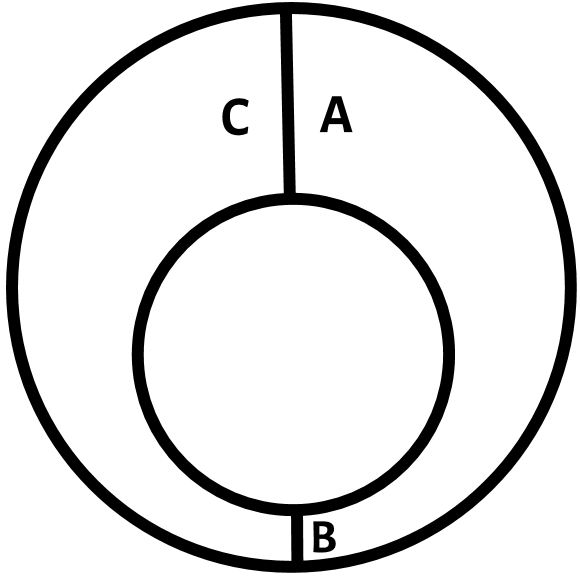
\includegraphics[width=1.25in,height=1.25in]{hegel-img002.png}
\end{center}
\item \label{bkm:Ref474665968}К стр. \pageref{bkm:bm48}. — Гегель дает здесь
в весьма вольном переводе и с перестановкой отдельных предложений
рассуждения Спинозы о бесконечном множестве неравных расстояний между двумя
неконцентричными окружностями (см. Спиноза, Переписка, М.~1932, стр.~78).
Конец приводимой Гегелем цитаты у Спинозы гласит: «...природа этой вещи не
может быть выражена никаким числом».
\item \label{bkm:Ref474666121}К стр. \pageref{bkm:bm49}. — В немецком тексте
вместо  стоит , а вместо  $(x+i)^n$ напечатано . Явная опечатка.
\item \label{bkm:Ref474666136}К стр. \pageref{bkm:bm50}. — Проверка с
помощью числа девять —~громоздкий искусственный прием, в настоящее время
вышедший из употребления, ввиду своей непрактичности.
\item \label{bkm:Ref474666147}К стр. \pageref{bkm:bm51}. — т.~е. «ведь эти
члены не будут иметь {\em никакого} значения» (или: «{\em никакого}
веса», «{\em никакой} силы»).
\item \label{bkm:Ref474666169}К стр. \pageref{bkm:bm52}. — См. стр.
\pageref{bkm:bm52a}–\pageref{bkm:bm52b}.
\item \label{bkm:Ref474666189}К стр. \pageref{bkm:bm53}. — Под
«Entwicklungspotenz» Гегель, как видно из этого места, а также из первого
абзаца следующего примечания («Еще другие формы, находящиеся в связи с
качественной определенностью величины», — стр. \pageref{bkm:bm53a}),
понимает то же самое, что в других местах он обозначает терминами:
«Entwicklungsglied» (член ряда, получающегося при разложении двучлена  по
формуле Ньютона), «Entwicklungsfunktion» (функция, получающаяся в
результате разложения в ряд, — «функция развертывания», как иногда
приходится переводить это выражение: см. напр. стр. \pageref{bkm:bm53b}),
«die Funktion der Potenzierung» (функция возвышения в степень),
«abgeleitete Funktion» (производная функция,— обычный в математике термин
для обозначения того, о чем здесь идет речь у Гегеля). Употребляя для
обозначения производной функции несколько странное выражение
«Entwicklungspotenz», Гегель, по-видимому, хочет подчеркнуть существенное
значение того обстоятельства, что дело идет тут именно о {\em степенных}
функциях, о разложении по {\em степеням}, о том, что интересующая нас
переменная величина {\em имеет степень выше первой} (см. выше, стр.
\pageref{bkm:bm53c}). Поэтому как первоначальную, так и производную функцию
Гегель называет «{\em степенными} функциями» (Potenzenfunktionen).
\end{enumerate}
В связи с этим нельзя не привести отзыв Энгельса. В письме Марксу от 18
августа 1881 г. Энгельс, говоря о математических рукописях Маркса, замечает
по поводу математических примечаний Гегеля: «Старик Гегель... вполне
правильно угадал, говоря, что дифференцирование в виде основного условия
требует, чтобы обе переменных имели различные степени и чтобы по меньшей
мере одна из них была во второй или $\frac 1 2$-й степени. Теперь мы уже знаем
почему». ({\em Маркс} и {\em Энгельс}, Соч., т.~XXIV, стр.~531–532).

\begin{enumerate}
\item \label{bkm:Ref474666244}К стр. \pageref{bkm:bm54}. — См. прим.
\ref{bkm:Ref474666189}.
\item \label{bkm:Ref474666256}К стр. \pageref{bkm:bm55}. — В немецком тексте
вместо «verglichen» стоит «vergleichen». По-видимому, это опечатка.
\item \label{bkm:Ref474666305}К стр. \pageref{bkm:bm56}. — Здесь слово «нуль»
употребляется Гегелем в фигуральном смысле —~в том смысле, что сторона
обратного отношения перестает быть стороной отношения, если она становится
равной показателю. В математическом же смысле, если мы возьмем обратное
отношение, показателем которого является произведение членов отношения  и
приравняем один из членов отношения этому произведению (например, ), то
другой член отношения будет не нулем, а единицей (у = 1). В арифметическом
обратном отношении (о котором здесь у Гегеля еще нет речи и формулой
которого является $х+у=С$), действительно, если $х=C$,
то $у=0$.
\item \label{bkm:Ref474666541}К стр. \pageref{bkm:bm57}. — В немецком тексте
вместо «keine» (никакой) стоит «eine». По-видимому, это опечатка.
\item \label{bkm:Ref474666560}К стр. \pageref{bkm:bm58}. — В издании Лассона
эта часть фразы дается по 1-му изданию «Науки логики», где эта фраза
гласит: «И вот определенное количество, которое отныне уже не есть
безразличное или внешнее определение, а дано так, что оно вместе с тем
снято как такое определение...» и~т.~д.
\item \label{bkm:Ref474666566}К стр. \pageref{bkm:bm59}. — Гегель имеет в
виду философию Шеллинга.
\item \label{bkm:Ref474666577}К стр. \pageref{bkm:bm60}. — Английское слово
«фут» означает прежде всего «нога, ступня», а затем уже «фут» в смысле меры
длины, приблизительно соответствующей длине ступни человека
(30,5~{\em см}). То же самое имеет место и в немецком языке со словом
«Fuss».
\item \label{bkm:Ref474666643}К стр. \pageref{bkm:bm61}. — Слово «правило»
(die Regel) Гегель употребляет здесь в смысле «мерило», «масштаб», «норма»,
«образцовая или указная мера» (Massregel, Richtmass). В XVIII в. слово
«Regel» иногда употреблялось в смысле линейки с делениями. Гегель,
по-видимому, и намекает на это старинное значение.
\item \label{bkm:Ref474666655}К стр. \pageref{bkm:bm62}. — Гегель
рассматривает здесь понятие физической {\em константы},~т.~е. того
эмпирического коэффициента, который в той или иной форме входит в уравнения
механики и физики. В качестве примера такой константы Гегель в следующей
фразе приводит величину $а$ в уравнении движения падения тел 
$s=at^2$. Гораздо чаще формулу движения падения тел
выражают уравнением $s=\frac 1 2 gt^2$, где константа
$g$ (постоянное для данного географического пункта ускорение силы
тяжести) равна приблизительно $9,8 \text{\em м}$ (в качестве единицы времени
берется при этом секунда). Следовательно, величина $а$ в уравнении
равна приблизительно $4,9 \text{\em м}$. Впрочем, надо сказать, что величина
$а$ или $g$, входящая в формулу движения падения тел, может
быть названа константою лишь в весьма относительном смысле. Дело в том, что
сама она изменяется с изменением расстояния от центра земного шара (а также
от расположения тяжелых масс на земной поверхности вблизи того места, где
производятся опыты с падением тел). Но так как эти изменения весьма
незначительны в тех случаях падения тел, которые рассматриваются в
элементарной механике (т.~е. в тех случаях, где расстояния, проходимые
падающим телом, незначительны по сравнению с длиной земного радиуса, причем
опыты производятся в одном и том же месте земной поверхности), то ими
вполне можно пренебречь.
\item \label{bkm:Ref474666676}К стр. \pageref{bkm:bm63}. — Здесь, как и в
предыдущем разделе «Мера как ряд отношений мер», Гегель имеет в виду учение
шведского химика Торберна Бергмана (1735–1784) о количественном выражении
сродства между основаниями и кислотами. Бергман предполагал, что одно и то
же количество какого-нибудь химического основания тем больше требует
кислоты для своего насыщения или нейтрализации, чем больше у них сродства
друг с другом. Он нашел, что для насыщения, например, 100 весовых частей
едкого кали требуется 78,5 весовых частей серной кислоты, или 64 весовых
частей азотной кислоты, или 51,5 весовых частей соляной кислоты и~т.~д.;
для насыщения же 100 весовых частей едкого натра нужно 177 весовых частей
верной кислоты, либо 135,5 весовых частей азотной кислоты, либо 125 весовых
частей соляной кислоты и~т.~д. В том и другом случае {\em порядок}
кислот остается {\em один и тот же}. Получается некоторой ряд пропорций
или мер насыщения (нейтрализации), который, по Гегелю, и характеризует
собой специфическую природу исследуемого вещества, выступающего в качестве
{\em противочлена} этого ряда. Учение Бергмана о химическом сродстве и
его количественном выражении было господствующей теорией в последней
четверти XVIII в. В начале XIX в. появилась новая теория химического
сродства, связанная с именем французского химика Клода Бертоллэ
(1748–1822), в значительной мере направленная против теории Бергмана.
Бертоллэ считал, что, наоборот, чем меньшее количество вещества $А$
требуется для нейтрализации вещества $В$, тем больше сродство между
ними. Кроме того, также и числовые значения мер насыщения, найденные
Бергманом, оказались при более тщательных экспериментах весьма неточными.
Сочинения Бергмана были изданы в немецком переводе в 1782–1799 гг. и были
широко известны в Германии. Между прочим, от Бергмана идет термин
«attractio electiva» (избирательное притяжение), который в немецком
переводе был передан термином «Wahlverwandtschaft» (избирательное
сродство), употребляемым здесь у Гегеля для обозначения одной из категорий
меры. Подробнее о теориях Бергмана и Бертоллэ см. у {\em Hermann Корр},
Geschichte der Chemie, Neudruck der Originalausgabe, Leipzig 1931, Bd. II,
S. 297–324, откуда и взяты вышеприведенные сведения. — Что касается
«избирательного сродства», как химической категории, то принцип этого
сродства был сформулирован еще задолго до Бергмана французским химиком
Этьеном Жоффруа (1672–1731), который в 1718 г. выставил следующее
положение: «Всякий раз, когда мы имеем соединение двух веществ, обладающих
склонностью соединяться друг с другом, если к этому соединению
примешивается третье вещество, имеющее более сильное сродство с одним из
первых двух, то это третье вещество соединяется с ним, отбивая его от
другого» (цитировано у Коппа, стр.~296 второго тома),~т.~е. указанное
третье вещество разлагает первоначально данное соединение, соединяясь с
одним из компонентов и вытесняя из соединения другой компонент.
\item \label{bkm:Ref474666698}К стр. \pageref{bkm:bm64}. — Имеется в виду
учение Бергмана (см. предыдущее примечание).
\item \label{bkm:Ref474666706}К стр. \pageref{bkm:bm65}. — «Учебник химии»
Берцелиуса вышел в трех томах в 1808–1828 гг.
\item \label{bkm:Ref474666715}К стр. \pageref{bkm:bm66}. — Гегель неправ:
причиной остановки маятника является не сила тяжести, а трение в том месте,
где маятник прикреплен или привязан, а также и сопротивление воздуха (или
какой-нибудь другой среды, в которой качается маятник).
\item \label{bkm:Ref474666719}К стр. \pageref{bkm:bm67}. — Немецкий текст
здесь испорчен. Перевод сделан на основе конъектуры Б. Г. Столпнера,
предлагающего вместо «eintretender qualitativer Bestimmtheit» читать
«eintretende qualitative Bestimmtheit». Лассон предлагает другую
конъектуру, вставляя перед указанными словами слова «ein Unterschied». В
этом случае надо было бы перевести эту фразу следующим образом: «Если,
таким образом, различие химического сродства, в противоположность
избирательному сродству, точно устанавливается в некотором ряде
количественных отношений, как различие появляющейся качественной
определенности...» и~т.~д.
\item \label{bkm:Ref474666725}К стр. \pageref{bkm:bm68}. — Имеются в виду
электрохимические теории английского химика Дэви (1778—1829) и шведского
химика Берцелиуса (1779–1848), явившиеся крупным шагом вперед в развитии
химии. Гегель недооценивал их значение, так же, как он недооценивал
прогрессивное значение химических теорий Бертоллэ.
\item \label{bkm:Ref474666740}К стр. \pageref{bkm:bm69}. — Выражение
«индифференция» (неразличенность, безразличие) было употреблено Шеллингом в
его вышедшей в 1801 г. работе «Изложение моей системы философии» для
обозначения «абсолютного тождества» субъекта и объекта. «Совершенная
неразличенность (totale Indifferenz) субъективного и объективного» —~таково
было основное понятие этой фазы философского развития Шеллинга. В
дальнейшем Гегель подробно рассматривает шеллинговскую концепцию
«индифференции как обратного отношения между ее факторами» и подвергает ее
имманентной критике, вскрывая ее «всестороннюю противоречивость». По учению
Шеллинга абсолютное представляет собою неподвижное тождество, полнейшую
неразличенность, совершенное безразличие двух факторов: субъективного и
объективного. Всякое же дифференцирование состоит лишь в количественном
перевесе одного из этих двух факторов над другим, причем «вечным основанием
и опорою всех количественных различий субъективного и объективного служит
их совершенная индифференция, составляющая форму абсолютного тождества,
форму их бесконечного бытия» (см. {\em Куно Фишер}, Шеллинг, его жизнь,
сочинения и учение, пер. H. Лocского, Спб. 1905, стр. 590). О шеллинговой
системе «абсолютного тождества» Гегель упоминал также и выше, на
стр.~\pageref{bkm:bm69a}. Ср. прим.~\ref{bkm:Ref474665876} к этому месту.
\item \label{bkm:Ref474666761}К стр. \pageref{bkm:bm70}. — См. предыдущее
примечание.
\item \label{bkm:Ref474666774}К стр. \pageref{bkm:bm71}. — В первом издании
«Науки логики» (1812) здесь стояла еще следующая фраза, выпущенная Гегелем
в 1831 г., когда он готовил второе издание: «Этот вопрос я осветил в моей
более ранней диссертации, где я доказал несостоятельность этого различения
и построенных на нем объяснений». Имеется в виду «Философская диссертация
об орбитах планет» (1801) Возможно, что Гегель выпустил эту ссылку на свою
диссертацию потому, что в ней, между прочим, доказывалось, что между
Юпитером и Марсом не может быть никаких планет, между тем как еще в 1801 г.
была открыта малая планета Церера, расположенная как раз между Юпитером и
Марсом.
\item \label{bkm:Ref474666782}К стр. \pageref{bkm:bm72}. — Это не совсем
так. Как уже было упомянуто в примечании \ref{bkm:Ref474665489}{}-м, Гегель
в значительной мере произвольно толковал философию Спинозы, приписывая ей
акосмизм (отрицание мира) и идеализм. В этом отношении он шел по стопам
Шеллинга, использовавшего некоторые элементы спинозизма для построения
своей идеалистической философии «абсолютного тождества». В действительности
же между материалистом Спинозой и объективным идеалистом Шеллингом огромная
принципиальная разница, и эта-то разница как раз и смазывается в
гегелевской трактовке спинозизма.
\item \label{bkm:Ref474666794}К стр. \pageref{bkm:bm73}. — См. «Учение о
бытии», стр. \pageref{bkm:bm73a}—\pageref{bkm:bm73b}.
\item \label{bkm:Ref474666798}К стр. \pageref{bkm:bm74}. — В немецком тексте
вместо sie (т.~е. Negation) стоит es. По-видимому, это опечатка.
\item \label{bkm:Ref474666813}К стр. \pageref{bkm:bm75}. — См. примечание
\ref{bkm:Ref474665836}.
\item \label{bkm:Ref474666829}К стр. \pageref{bkm:bm76}. — См.
{\em Кант}, Критика способности суждения, пер. Н. Соколова, Спб. 1898,
стр. 16—17.
\item \label{bkm:Ref474666833}К стр. \pageref{bkm:bm77}. — Здесь кончается
выписка из «Критики способности суждения» (стр. XXVI немецкого издания 1799
г., стр.~16 русского перевода).
\item \label{bkm:Ref474666843}К стр. \pageref{bkm:bm78}. — Гегель имеет в
виду Шеллинга и его последователей. Шеллинг начиная с 1800 г., когда он
выпустил свою «Систему трансцендентального идеализма», выдвигает в качестве
«органа всякого трансцендентального мышления» «интеллектуальную интуицию»,
как непосредственное созерцание абсолютного, целиком противоположное
рассудочному познанию и совершенно оторванное от него. Против шеллинговой
«интеллектуальной интуиции» Гегель впервые выступил в начале 1807 г в
предисловии к «Феноменологии духа». В своих «Лекциях по истории философии»
Гегель дает более развернутую критику Шеллинга и его поклонников. Особенно
резко он отзывается об этих последних. «Вся эта тенденция, — говорит он об
антинаучном характере философских упражнений шеллингианцев, —
противопоставляет себя прежде всего {\em рефлективному мышлению}, или,
иначе сказать, такому движению рассуждения, которое держится фиксированных,
прочных, неподвижных понятий. Но вместо того чтобы оставаться в области
понятия и познать его как беспокойное «я», они впали в противоположную
крайность покоящегося созерцания, непосредственного бытия, неподвижного «в
себе» и полагают, что этот недостаток, эта неподвижность, исправляется
глядением и что это глядение они превращают в интеллектуальное, определяя
его в свою очередь посредством какого-нибудь фиксированного понятия»
({\em Гегель}, Лекции по истории философии, кн.~III. М.—Л. 1936,
стр.~511).
\end{enumerate}
Самое слово «рефлексия» Гегель употребляет в различных значениях, притом
так, что одно значение незаметно переходит у него в другое или даже
совмещается с другим. Латинское слово «reflexio» означает «загибание назад,
отклонение назад, отражение» (света, звуковой волны, брошенного во
что-нибудь предмета). В новых языках это слово наряду с этим значением
«отражения» приобрело еще значение «размышления, обдумывания, рассуждения,
соображения, рассудительности» (мысль как бы оборачивается на самоё себя,
отражается в себя самоё). У Гегеля рефлексия берется то в объективном, то в
субъективном смысле. При этом Гегель, как объективный и абсолютный
{\em идеалист}, понимает объективную рефлексию не в смысле взаимного
отражения сторон или моментов материального предмета друг другом или друг в
друге и не в смысле обратного их отражения в себя самих, а в смысле
взаимного отражения между определениями понятия как такового или в смысле
обратного отражения какого-нибудь понятийного определения внутрь себя
самого («рефлексия в себя»). Субъективную же рефлексию Гегель, как
идеалист, берет не в смысле гносеологического отражения объективно-реальной
материальной действительности в человеческом или животном сознании, а в
смысле рассудочного оперирования абстрактными категориями чистой мысли.
Рефлексия рассудка подвергается у Гегеля уничтожающей критике в том случае,
если она выступает с претензией на полное, завершенное, абсолютное
познание. Но вместе с тем Гегель решительно защищает эту рефлексию рассудка
как необходимый момент в диалектическом развитии познания (против Шеллинга
и шеллингианцев, против Якоби и против романтиков). Рефлексия в себя и
рефлексия в другое (притом не в другое вообще, а в «{\em свое} другое»)
составляют, по Гегелю, характерную черту категорий сущности (которая ведь
представляет собою «абсолютное опосредствование с собою»), точно так же как
переход от одного к другому был характерной чертой категорий бытия (где
господствует непосредственность), а развитие или развертывание
(Entwickelung) будет характерной чертой категорий понятия (где имеет место
единство непосредственного и опосредствованного).

В теснейшей связи с выражением «рефлексия» Гегель употребляет выражение
«Scheinen», имеющее у него опять-таки специфически-метафорическое значение.
«Das Scheinen» означает у Гегеля «свечение, мерцание, отблеск» (например,
Гегель говорит, что положительное «светится» в отрицательном, а
отрицательное —~в положительном; см. в тексте стр. \pageref{bkm:bm78a}).
Иногда Гегель приводит выражение «Scheinen» в прямою связь с термином
«Schein» (видимость, кажимость), и тогда «das Scheinen» приходится
переводить словами «свечение видимостью» (в себе самом или в своем другом),
или «излучение видимости» (в себя самого или в свое другое).

\begin{enumerate}
\item \label{bkm:Ref474666865}К стр. \pageref{bkm:bm79}. — В немецком тексте
(как в издании Глокнера, так и в издании Лассона) вместо слова
«положительным» стоит слово «отрицательным». По-видимому, это опечатка.
\item \label{bkm:Ref474666880}К стр. \pageref{bkm:bm80}. — В немецком тексте
наоборот: «+~а раз –~а». По-видимому, это опечатка.
\item \label{bkm:Ref474666891}К стр. \pageref{bkm:bm81}. — Об игре слов в
немецком выражении «zu Grunde gehen», как его употребляет Гегель, см.
замечания Энгельса в письмах Конраду Шмидту от 1 ноября 1891 г. и от 4
февраля 1892 г. ({\em Маркс} и {\em Энгельс}, Письма, под ред.
Адоратского, изд. 4-е, М.—Л. 1931, стр. 393–394).
\item \label{bkm:Ref474666904}К стр. \pageref{bkm:bm82}. — Слово «этиология»
(от греческого «aitia» —~причина, начало, основание) означает учение о
причинах, указание причин или оснований для тех или иных явлений.
\item \label{bkm:Ref474666911}К стр. \pageref{bkm:bm83}. — Лассон считает,
что придаточное предложение «что растение имеет свое основание в
производящей растения силе» попало сюда по ошибке и должно быть поставлено
двумя строчками выше, после слов «я скажу, что оно есть растение».
Стилистически такая перестановка улучшает конструкцию всей этой фразы, но
логический смысл заставляет предпочесть тот текст, какой дается в издании
Глокнера. С этого текста и сделан перевод этой фразы с добавлением слов
«того предложения» перед приведенным выше придаточным предложением.
\item \label{bkm:Ref474666923}К стр. \pageref{bkm:bm84}. — т.~е. по-своему,
по-разному.
\item \label{bkm:Ref474666940}К стр. \pageref{bkm:bm85}. — См. «Учение о
бытии», стр. \pageref{bkm:bm85a}–\pageref{bkm:bm85b}.
\item \label{bkm:Ref474667017}К стр. \pageref{bkm:bm86}. — В русском
переводе под ред. Радлова ({\em Гегель}, Феноменология духа, Спб. 1913)
это место находится на стр. 72—74 (в главе «Сила и рассудок, явление и
сверхчувственный мир»).
\item \label{bkm:Ref474667030}К стр. \pageref{bkm:bm87}. — В немецком
тексте: «das Relative eines Ändern». По-видимому, это опечатка вместо: «das
Relative seines Ändern».
\item \label{bkm:Ref474667041}К стр. \pageref{bkm:bm88}. — См. часть первая,
стр. \pageref{bkm:bm88a}–\pageref{bkm:bm88b}.
\item \label{bkm:Ref474667057}К стр. \pageref{bkm:bm89}. — В немецком
тексте: «in derselben». По-видимому, это опечатка вместо: «in demselben».
\item \label{bkm:Ref474667072}К стр. \pageref{bkm:bm90}. — Ср. замечание
Энгельса о том, что «сила имеет точно такую же величину, как и ее
проявление во-вне, ибо в них обоих совершается {\em одно и то же
движение}» ({\em Engels}, Herrn E. Dührings Umwälzung der Wissenschaft.
Moskau —~Leningrad 1935, S.~64).
\item \label{bkm:Ref474669620}К стр. \pageref{bkm:bm91}. — См. примечания
\ref{bkm:Ref474665489} и \ref{bkm:Ref474666782}.
\item \label{bkm:Ref474669634}К стр. \pageref{bkm:bm92}. — Это не точно. 4-я
дефиниция первой части «Этики» гласит: «Под атрибутом я разумею то, что
интеллект мыслит о субстанции, как составляющее ее сущность». Из
сопоставления этой дефиниции с рядом других мест из «Этики» и из
«Переписки» Спинозы видно, что атрибуты, но учению Спинозы, не только
{\em мыслятся} интеллектом как составляющие сущность субстанции, но и
действительно «выражают, раскрывают и составляют вечную сущность и вечное
существование» субстанции безотносительно к интеллекту (см., например,
доказательства теоремы 19-й и 20-й первой части «Этики» и письмо 2-е).
Субстанция, говорит Спиноза, {\em имеет} атрибуты (доказательство
теоремы 16-й первой части «Этики»).
\item \label{bkm:Ref474669669}К стр. \pageref{bkm:bm93}. — Абсолютная
необходимость слепа потому, что она равносильна абсолютной случайности, как
это более определенно намечается Гегелем в непосредственно следующих за
этим рассуждениях, содержащих элементы диалектической критики категории
абсолютной необходимости. Если все одинаково абсолютно-необходимо, если
все, что существует, существует только потому, что оно существует, не имея
для своего существования никаких других оснований, то это значит, что все
абсолютно случайно. Здесь получается {\em непосредственное} или, как
выражается Гегель, намекая, по-видимому, на Шеллинга (а также, без сомнения,
и на метафизический детерминизм Спинозы), «{\em абсолютное}» тождество
сущности и бытия, возможности и действительности, необходимости и
случайности —~такое тождество, где отсутствует самодвижение, где имеется
лишь «рефлексия в себя» без «рефлексии в другое». Сама сущность выступает
здесь в форме «бытия», в форме простой непосредственности, простого факта.
Подобно тому, как ночью, согласно немецкой поговорке, «все коровы черны»
(или, согласно русской поговорке, «все кошки серы»), так и в «одноцветном»
абсолюте Шеллинга все совершенно одинаково {\em по своей форме}, все
различия между отдельными категориями стерты, растворены в «пустой бездне»
({\em Гегель}, Феноменология духа, предисловие, стр. 12 в немецком
издании Лассона, Лейпциг 1921, или стр. 7 в русском переводе под ред.
Радлова, Спб. 1913). Что касается специально абсолютной необходимости, то
возможность абсолютно-необходимого и его действительность непосредственно
совпадают именно потому, что все вещи и все события рассматриваются на
данном этапе как {\em одинаково} необходимые, как необходимости
{\em одного и того же порядка}. Ср. классические формулировки Спинозы:
«Из необходимости божественной природы должно следовать бесконечно многое
бесконечно-многими способами,~т.~е. все то, что может стать объектом
бесконечного интеллекта» («Этика», ч.~I, теор.~16); «из бесконечной природы
бога все всегда следует по одной и той же необходимости, точно таким же
образом, как из природы треугольника от века и до века следует, что его три
угла равны двум прямым» (там же, схолия к теор. 17). По Спинозе, все
отдельные вещи одинаково необходимы, но вместе с тем все они одинаково
случайны (см. королларий к теор. 31 второй части и дефиницию 3-ю четвертой
части).
\end{enumerate}
В своем гениальном отрывке о «Случайности и необходимости» Энгельс, отмечая
заслуги Гегеля по части диалектической трактовки категорий необходимости и
случайности, дает замечательный по своей глубине и ясности диалектический
анализ и диалектическую критику точки зрения абсолютной необходимости,
которую он характеризует как «механический детерминизм, который на словах
отрицает случайность в общем, чтобы на практике признать ее в каждом
отдельном случае» («Диалектика природы», изд. 1936 г., стр. 109).
Механический детерминизм, указывает Энгельс, «деградирует необходимость до
уровня случайности» (там же, стр. 108).

Известное положение Гегеля о том, что «слепа необходимость лишь постольку,
поскольку она не постигается в понятии» ({\em Гегель}, Собр. соч., т. I,
стр. 248; ср. {\em Энгельс}, Анти-Дюринг, гл. XI первого раздела),
нисколько не противоречит его трактовке абсолютной необходимости в
рассматриваемом месте, ибо абсолютная необходимость, провозглашаемая
механическим детерминизмом, по самому существу своему не может быть
объектом конкретного, адэкватного познания, не может быть «постигнута в
понятии». Поэтому Гегель и говорит, что в стадии абсолютной необходимости
(или, что то же самое, в стадии абсолютной действительности, абсолютного
факта) необходимость «заперта» в бытии, что она «боится света». В
дальнейшем, а именно при переходе от «Сущности» к «Понятию», необходимость
«раскроется» (ср. в тексте стр. \pageref{bkm:bm93a}) и тем самым перестанет
быть «слепой».

\begin{enumerate}
\item \label{bkm:Ref474669698}К стр. \pageref{bkm:bm94}. — Это предисловие
предпослано IV т. Собрания сочинений Гегеля, изданного вскоре после его
смерти его учениками, — тому, содержащему 2-ю часть «Науки логики»
—~«Учение о сущности».
\item \label{bkm:Ref474655210}К стр. \pageref{bkm:bm95}. — Имеется в виду
изречение Лессинга о том, что если бы бог предложил ему выбор между
готовой, законченной, чистой истиной и вечно живым стремлением к ней,
стремлением, связанным с постоянными ошибками и заблуждениями, то он выбрал
бы последнее. См. Lessings Philosophie, hrsg. von Paul Lorenz, Leipzig
1909, S. 106.
\end{enumerate}

\bigskip


\bigskip



\clearpage
\tableofcontents*
\clearpage

\end{document}
